\documentclass[10pt,a4paper,twoside,openany]{book}
\usepackage[
  a4paper,
  top=22mm,
  bottom=23mm,
  inner=22mm,
  outer=23.5mm,
  marginparwidth=16.5mm,
  marginparsep=3.5mm
]{geometry}
\usepackage{fontspec}
\usepackage{xeCJK}
\usepackage{amsmath,amssymb}
\usepackage{tikz-cd}
\usetikzlibrary{decorations.pathmorphing}
\usepackage{enumitem}
\usepackage[hidelinks,unicode,hypertexnames=false]{hyperref}
\usepackage{microtype}
% Shared continuous-reading layout for the Chinese and Japanese editions.
% The source-page-mirrored main.tex files remain the archival editions.
\RequirePackage{xcolor}
\RequirePackage{marginnote}
\RequirePackage{marginfix}
\RequirePackage{needspace}

\setlength{\marginparpush}{5pt}
\emergencystretch=1.5em
\providecommand{\marginfont}{}
\renewcommand*{\marginfont}{\scriptsize\sffamily\color{gray}}

\providecommand{\VerdierSourcePageLabel}[1]{source p.~#1}
\providecommand{\VerdierSourceRomanLabel}[1]{source p.~#1}
\providecommand{\VerdierSourcePdfLabel}[1]{source PDF p.~#1}
\newcommand{\VerdierSemanticAnchor}[1]{%
  \hypertarget{verdier-semantic-#1}{}% 
}
\newcommand{\VerdierPhysicalPageAnchor}[1]{%
  \hypertarget{verdier-physical-#1}{}% 
}

\newcommand{\VerdierSourcePageNote}[1]{%
  \marginnote{%
    \ifodd\value{page}\raggedright\else\raggedleft\fi
    \marginfont
    \ifnum#1<6
      \VerdierSourcePdfLabel{\number\numexpr#1\relax}%
    \else\ifnum#1<15
      \VerdierSourceRomanLabel{\romannumeral\numexpr#1-5\relax}%
    \else\ifnum#1<18
      \VerdierSourcePdfLabel{\number\numexpr#1\relax}%
    \else
      \VerdierSourcePageLabel{\number\numexpr#1-17\relax}%
    \fi\fi\fi
  }% 
}

% A hard source boundary has already flushed floats before this command.  Use
% the class's unnumbered chapter heading without its second, redundant clear.
\newcommand{\VerdierReaderChapterStar}[1]{%
  \begingroup
    \let\clearpage\relax
    \let\cleardoublepage\relax
    \chapter*{#1}%
  \endgroup
}

% A block milestone begins a genuine new paragraph or block in the source.
\newcommand{\VerdierSourcePageBlock}[1]{%
  \VerdierPhysicalPageAnchor{#1}%
  \VerdierSourcePageNote{#1}%
  \ignorespaces
}

% A continuation milestone occurs inside the same source paragraph.
\newcommand{\VerdierSourcePageContinue}[1]{%
  \VerdierPhysicalPageAnchor{#1}%
  \VerdierSourcePageNote{#1}%
  \ignorespaces
}

% Blank authority pages keep a machine destination but create neither a
% visible note nor a blank page in the continuous-reading edition.
\newcommand{\VerdierSourcePageSilent}[1]{%
  \VerdierPhysicalPageAnchor{#1}%
  \ignorespaces
}

% Natural-size commutative diagrams must never be stranded below the text
% block.  The generator inserts this only at independently identified tall
% Japanese diagrams; the source modules and mathematical labels stay intact.
\newcommand{\VerdierReaderDiagramPageFit}{%
  \par\Needspace{18\baselineskip}%
}


\setmainfont{Noto Serif}
\setsansfont{Noto Sans}
\setCJKmainfont[
  BoldFont=Yu Gothic,
  ItalicFont=Yu Gothic,
  BoldItalicFont=Yu Gothic,
  ItalicFeatures={FakeSlant=0.18},
  BoldItalicFeatures={FakeSlant=0.18}
]{Yu Gothic}
\setCJKsansfont[BoldFont=Yu Gothic]{Yu Gothic}
\XeTeXlinebreaklocale "ja"
\XeTeXlinebreakskip=0pt plus 1pt
\setlength{\parindent}{1em}
\setlength{\parskip}{0.15em}
\setlist[description]{style=multiline,labelwidth=2.6em,leftmargin=3.2em,itemsep=0.25em,parsep=0pt,topsep=0.25em}

\renewcommand{\VerdierSourcePageLabel}[1]{原典 p.\,#1}
\renewcommand{\VerdierSourceRomanLabel}[1]{原典 p.\,#1}
\renewcommand{\VerdierSourcePdfLabel}[1]{原典 PDF p.\,#1}
\newcommand{\LocalizedChapterLabel}{第\kern0pt\thechapter\kern0pt章}
\makeatletter
\renewcommand{\chaptermark}[1]{\markright{\LocalizedChapterLabel\quad #1}}
\renewcommand{\@makechapterhead}[1]{%
  \vspace*{50\p@}%
  {\parindent \z@ \raggedright \normalfont
    \ifnum \c@secnumdepth >\m@ne
      \if@mainmatter
        \huge\bfseries \LocalizedChapterLabel\par\nobreak
        \vskip 20\p@
      \fi
    \fi
    \interlinepenalty\@M
    \Huge\bfseries #1\par\nobreak
    \vskip 40\p@
  }}
\makeatother

\title{アーベル圏の導来圏}
\author{Jean-Louis Verdier}
\date{1996}
\hypersetup{
  pdftitle={アーベル圏の導来圏},
  pdfauthor={Jean-Louis Verdier},
  pdfsubject={日本語連続閲覧版；原典ページのマイルストーンを保持}
}

\begin{document}
\pagenumbering{roman}
% GENERATED by qa/build_cjk_reader_streams.py; DO NOT EDIT.
% Continuous preliminary matter with complete source milestones.
\VerdierSemanticAnchor{front-title}
\begin{titlepage}
  \VerdierSourcePageBlock{0002}
  \centering
  {\Huge\bfseries 239\hfill ASTÉRISQUE\par}
  \vspace{1.5em}
  {\LARGE\bfseries 1996\par}
  \vfill
  {\Huge\bfseries アーベル圏の\par}
  \vspace{0.4em}
  {\Huge\bfseries 導来圏\par}
  \vspace{3em}
  {\Large\bfseries Jean-Louis VERDIER\par}
  \vfill
  {\Large\bfseries フランス数学会\par}
  \smallskip
  {\small\bfseries フランス国立科学研究センターの助成により刊行\par}
\end{titlepage}

\clearpage
\VerdierSemanticAnchor{front-ams-classification}
\VerdierSourcePageBlock{0003}
\VerdierReaderChapterStar{AMS 主題分類}
\addcontentsline{toc}{chapter}{AMS 主題分類}

14F20, 18E30, 18E35, 18G05, 18G10, 18G15, 18G20, 18G35,
18G40, 55U15, 55U25, 55U30.

\clearpage
\VerdierSemanticAnchor{front-portrait}
\VerdierSourcePageBlock{0004}
\thispagestyle{empty}
\vspace*{0.62\textheight}
\begin{center}
Jean-Louis VERDIER、1977年
\end{center}

\VerdierSourcePageSilent{0005}%
\clearpage
\VerdierSemanticAnchor{front-preface}
\VerdierSourcePageBlock{0006}
\VerdierReaderChapterStar{序文}
\addcontentsline{toc}{chapter}{序文}

1989年8月25日に悲劇的な死を遂げた Jean-Louis Verdier は、1967年6月14日、
パリにおいて『アーベル圏の導来圏』と題する国家博士論文の審査を受けた。
本書のテキストは、この論文のタイプ原稿の最終版である。編者が行ったのは細部
の誤りを訂正することに限られる。学部に提出されていたのは「序論」と題する
部分だけであり、本文は審査時にも未完で、その後も未完のままであった。

この仕事の成立事情はかなりよく知られている（\emph{参照} [I]）。
Grothendieck は1960年代初頭、1958年のエディンバラ国際数学者会議での講演を
受けて構想していた双対性定理の大規模な一般化に必要なホモロジー代数の枠組み
を与えるため、導来圏という着想を得た。彼は Verdier に、その形式体系の構築
を博士論文の課題として提案した。1963年、Verdier は理論の本質的内容を要約
した成果集『導来圏、いくつかの結果（状態0）』を IHÉS の謄写版として刊行した
（[SGA 4 1/2] に再録）。導来圏の概念は Grothendieck に由来するが、それに
先立って三角圏の概念を導入したのは Verdier である。安定ホモトピー論に着想
を得たそこでの公理的枠組み（\emph{参照} [P]）は、驚くほど豊かな成果をもたらす
ことになった。

Verdier が自らの仕事を包括的に記述し始めたのは、それから何年も後のことで
ある。なぜ完成させなかったのか。多くの仮説が唱えられてきたが、私は次の説明
に傾く。欠けている部分は導来関手の理論である。Verdier がそこまで書き進めた
頃には、導来圏はすでに代数幾何で広く使われ、さまざまな変形と一般化が発展
していた。Deligne 流の各点での導来可能性、非加法的導来関手（Quillen 流の
ホモトピー代数）、フィルター付き導来関手などである。その時点で、成果集が
定めた枠組みは不十分になっていた。適切な観点を見いだすには新たな基礎研究が
必要だったが、当時ほかの問題に関心を向けていた Verdier には、その余裕も、
おそらく意欲もなかったのだと私は思う。時がたつにつれ導来圏に関する論文が
現れ、その利用は広がり、形式体系は数学の別分野（たとえば線形偏微分方程式）
にも浸透した。こうして Verdier の目には、この仕事を完成させることがますます
不要に映るようになったのである……。

\VerdierSourcePageBlock{0007}
未完ではあるものの、Verdier のこのテキストは貴重で、まさに代えがたい参考
文献である（たとえば、ここに示されたスペクトル系列の独創的で優美な提示は、
私の知る限りほかのどこにも見られない）。それがついに日の目を見たことを、
心から喜びたい。

\begin{flushright}
パリ、1996年4月27日\\
Luc Illusie
\end{flushright}

\section*{参考文献}

\begin{description}[labelwidth=6.2em,leftmargin=6.8em]
\item[{[I]}] L. Illusie, \emph{Catégories dérivées et dualité, travaux de
J.-L. Verdier}, L'Enseignement Mathématique, 36 (1990), 369--391.
（1989年10月19日、Université Paris VII 主催の Jean-Louis Verdier 追悼式
における講演。）

\item[{[P]}] D. Puppe, \emph{On the formal structure of stable homotopy
theory}, Colloquium on Algebraic Topology, Aarhus Universitet (1962),
65--71.

\item[{\mbox{[SGA 4 1/2]}}] ``Cohomologie étale'', Séminaire de Géométrie
Algébrique du Bois-Marie, SGA 4 1/2, P. Deligne, Lecture Notes in
Mathematics 569, Springer-Verlag (1977), 262--311.
\end{description}
\clearpage
\VerdierSemanticAnchor{front-editors-note}
\VerdierSourcePageBlock{0008}
\VerdierReaderChapterStar{編者注}
\addcontentsline{toc}{chapter}{編者注}

\VerdierSemanticAnchor{front-editors-note-publication-history}
J.-L. Verdier を追悼して Université Paris VII が1989年10月19日に催した式典
において、M. Artin、P. Cartier、L. Illusie は J.-L. Verdier の博士論文を
出版する着想を得た。2年後、私も彼らに加わり、J. Le Potier と M. Broué の
支援を得て、本文を \TeX{} に入力するための資金を Paris VII（URA 212）と
ÉNS（DMI）から確保した。入力完了後、その結果を Verdier のタイプ原稿と入念
に照合した。しかし Verdier 自身が最終訂正を行っていなかったため、数学的な
校閲がなお必要であった。

\VerdierSemanticAnchor{front-editors-note-chapter-i-modifications}
この精密な校閲は、P. Cartier（第I章）、B. Keller（第III章）、そして全文に
ついては M. Zisman と私が、細心の注意を払って行った。列挙するほどでもない
多数の誤植を除けば、主な変更は次のとおりである。第I章の命題 (3.1.5) は同値
を主張していた。この逆向き（後では一度も使われない）が偽なので、同値を含意
に置き換えた。命題 (3.4.1) には符号の誤りがあり、第III章 ((1.3.4)、(b)、
(3.2.7.3)) の符号の誤りを引き起こしていた。そのため「反対三角圏」
（第II章、1.1.7）の定義を調整し、次の主張が真であり続けるようにした：
\emph{反対圏の導来圏は、元の導来圏の反対三角圏である}。

\VerdierSemanticAnchor{front-editors-note-chapter-ii-modifications}
第II章では、§1.2 の命題の順序を変更した。Verdier は執筆後、二つの完全三角
の直和が完全三角になるという主張は三角圏の他の公理から従うことに気づいて
いた。そのため公理の一覧からは削除したが、それに伴う再配列を行っていなかった
のである。さらに、後で使われず、検証にも失敗した段落 (2.3.6) と (2.3.7) を
削除した。定常スペクトル対象 (4.4.2) の定義はわずかに修正した。元の定義では
弱すぎて、後続の定理 (4.4.3) を証明できなかったためである。この変更が以後
の内容に影響しないことも確認した。

\VerdierSourcePageBlock{0009}
\VerdierSemanticAnchor{front-editors-note-apparatus}
記号索引と用語索引は補完した。一方、参考文献は変更しなかった（ただし SGA
各巻については ``Lecture Notes'' での確定書誌情報を示した）。とりわけ、
参考文献番号13の欠落は補っていない。

\VerdierSemanticAnchor{front-editors-note-acknowledgements}
この企画の実現をさまざまな形で助けてくださった M. Broué、A. Bruguières、
P. Cartier、L. Gruson、L. Illusie、B. Keller、J. Le Potier、M. Zisman、
ならびに Université Paris VII、École Normale Supérieure、Institut des
Hautes Études Scientifiques に心から感謝したい。また、本書を辛抱強く
\textsc{AMS}-\TeX{} に入力してくださった C. Defosse と C. Gourgues にも
感謝する。

\VerdierSemanticAnchor{front-editors-note-memorial}
1994年12月に早逝した L. Doustaing にも、この感謝を伝えたかった。

\VerdierSemanticAnchor{front-editors-note-signature}
\begin{flushright}
パリ、1996年6月14日\\
Georges Maltsiniotis
\end{flushright}
\clearpage
\VerdierSemanticAnchor{front-publications}
\VerdierSourcePageBlock{0010}
\VerdierReaderChapterStar{J.-L. Verdier 著作目録}
\addcontentsline{toc}{chapter}{J.-L. Verdier 著作目録}

\small
\begin{description}
\VerdierSemanticAnchor{front-publications-01}
\item[{[01]}] \emph{保型形式に付随する積分について}（G. Shimura による）、
Séminaire Bourbaki 1960--61, no. 216, pp. 216-1--216-27,
Benjamin (1966).

\VerdierSemanticAnchor{front-publications-02}
\item[{[02]}] \emph{Poincaré 双対定理}, C.R.A.S. vol. 256,
pp. 2084--2086, Gauthier-Villars (1963).

\VerdierSemanticAnchor{front-publications-03}
\item[{[03]}] \emph{数体のエタール・コホモロジーに関するセミナー}
（M. Artin との共著）, Woods Hole Conference on Algebraic Geometry,
A.M.S. (1964).

\VerdierSemanticAnchor{front-publications-04}
\item[{[04]}] \emph{射影系の本質的同値}, C.R.A.S. vol. 261,
pp. 4950--4953, Gauthier-Villars (1965).

\VerdierSemanticAnchor{front-publications-05}
\item[{[05]}] \emph{局所コンパクト空間の次元}, C.R.A.S. vol. 261,
pp. 5293--5296, Gauthier-Villars (1965).

\VerdierSemanticAnchor{front-publications-06}
\item[{[06]}] \emph{副有限群のコホモロジーにおける双対性}, Jean-Pierre
Serre, ``Galois Cohomology'' の付録, Lecture Notes in Mathematics 5,
pp. 183--206, Springer (1964), 第4版 (1973).

\VerdierSemanticAnchor{front-publications-07}
\item[{[07]}] \emph{局所コンパクト空間上の構成可能層}, C.R.A.S. vol. 262,
pp. 12--15, Gauthier-Villars (1966).

\VerdierSemanticAnchor{front-publications-08}
\item[{[08]}] \emph{局所コンパクト空間のコホモロジーにおける双対性},
Séminaire Bourbaki 1965--66, no. 300, pp. 300-01--300-13,
Benjamin (1966).

\VerdierSemanticAnchor{front-publications-09}
\item[{[09]}] \emph{エタール・コホモロジーにおける Lefschetz 不動点公式},
Conference on Local Fields, 1966年 Driebergen の NUFFIC Summer School,
pp. 199--214, Springer (1967).

\VerdierSemanticAnchor{front-publications-10}
\item[{[10]}] \emph{スキームのエタール・コホモロジーにおける双対定理},
Conference on Local Fields, 1966年 Driebergen の NUFFIC Summer School,
pp. 184--198, Springer (1967).

\VerdierSemanticAnchor{front-publications-11}
\item[{[11]}] \emph{連接層のねじれ逆像に対する基底変換}, Bombay
Colloquium on Algebraic Geometry in 1968, pp. 393--408, Oxford
University Press (1969).
\end{description}
\normalsize
\VerdierSourcePageContinue{0011}
\small
\begin{description}
\VerdierSemanticAnchor{front-publications-12}
\item[{[12]}] \emph{局所コンパクト空間のコホモロジーに対する双対定理},
Poincaré Duality, Heidelberg-Strasbourg Seminar 1966--67, exp. 4,
Publ. I.R.M.A. Strasbourg, no. 3, pp. 1--36 (1969).

\VerdierSemanticAnchor{front-publications-13}
\item[{[13]}] \emph{核定理}, Poincaré Duality, Heidelberg-Strasbourg
Seminar 1966--67, exp. 9, Publ. I.R.M.A. Strasbourg, no. 3,
pp. 1--52 (1969).

\VerdierSemanticAnchor{front-publications-14}
\item[{[14]}] \emph{Wilder の定理について}, Applications of categorical
algebra, Proc. Symp. Pure Math. 17, pp. 184--191, A.M.S. (1970).

\VerdierSemanticAnchor{front-publications-15}
\item[{[15]}] \emph{Grauert の連接性定理の簡明な証明}（R. Kiehl との共著）, 
Math. Ann. 195, pp. 24--50, Springer (1971).

\VerdierSemanticAnchor{front-publications-16}
\item[{[16]}] \emph{連接コホモロジーをもつ解析層複体のコホモロジー空間上の
位相}, Bull. Soc. Math. France 99, pp. 337--343, Gauthier-Villars
(1971).

\VerdierSemanticAnchor{front-publications-17}
\item[{[17]}] \emph{複素解析幾何における相対双対性}（J.-P. Ramis、
G. Ruget との共著）, Inv. Math. 13, pp. 261--283, Springer (1971).

\VerdierSemanticAnchor{front-publications-18}
\item[{[18]}] S.G.A. 4 (1963--64)「トポスの理論とスキームのエタール・
コホモロジー」：\emph{前層}（A. Grothendieck との共著）, pp. 1--184；
\emph{位相と層}, pp. 219--263；\emph{層の圏の関手性}, pp. 265--297；
\emph{トポス}（A. Grothendieck との共著）, pp. 299--519,
Lecture Notes in Mathematics 269, Springer (1972).

\VerdierSemanticAnchor{front-publications-19}
\item[{[19]}] S.G.A. 4 (1963--64)「トポスの理論とスキームのエタール・
コホモロジー」：\emph{トポスにおけるコホモロジー}, pp. 1--62；
\emph{有限性条件、ファイバー化トポスとサイト、および極限移行問題への応用}
（A. Grothendieck との共著）, pp. 163--336, Lecture Notes in
Mathematics 270, Springer (1972).

\VerdierSemanticAnchor{front-publications-20}
\item[{[20]}] \emph{Euler-Poincaré 標数}, Bull. Soc. Math. France 101,
pp. 441--445, Gauthier-Villars (1973).

\VerdierSemanticAnchor{front-publications-21}
\item[{[21]}] \emph{Le Potier の定理}, Seminar on Analytic Geometry
1972--73, Various aspects of positivity, Astérisque 17, pp. 68--78,
S.M.F. (1974).

\VerdierSemanticAnchor{front-publications-22}
\item[{[22]}] \emph{$l$ 進コホモロジーの Frobenius 自己準同型の特性多項式
の $l$ からの独立性}（P. Deligne による）, Séminaire Bourbaki
1972--73, no. 423, Lecture Notes in Mathematics 383, pp. 98--115,
Springer (1974).

\VerdierSemanticAnchor{front-publications-23}
\item[{[23]}] \emph{Riemann 幾何におけるいくつかの交叉問題}
（P. Marry との共著）, J. Diff. Geom. 12, pp. 345--376, A.M.S. (1977).
\end{description}
\normalsize
\VerdierSourcePageContinue{0012}
\small
\begin{description}
\VerdierSemanticAnchor{front-publications-24}
\item[{[24]}] \emph{Whitney 層化と Bertini-Sard 定理}, Inv. Math. 36,
pp. 295--312, Springer (1976).

\VerdierSemanticAnchor{front-publications-25}
\item[{[25]}] \emph{サイクルに付随するホモロジー類}, Seminar on
Analytic Geometry 1974--75, Astérisque 36--37, pp. 101--151,
S.M.F. (1976).

\VerdierSemanticAnchor{front-publications-26}
\item[{[26]}] \emph{完全交叉に対する Riemann-Roch 定理}, Seminar on
Analytic Geometry 1974--1975, Astérisque 36--37, pp. 189--228,
S.M.F. (1976).

\VerdierSemanticAnchor{front-publications-27}
\item[{[27]}] \emph{特異点をもちうる代数多様体に対する Riemann-Roch 定理}
（P. Baum、W. Fulton、R. MacPherson による）, Séminaire Bourbaki
1974--75, no. 464, Lecture Notes in Mathematics 514, pp. 159--175,
Springer (1976).

\VerdierSemanticAnchor{front-publications-28}
\item[{[28]}] \emph{導来圏}（1963年執筆、1976年刊行）, Seminar on
Algebraic Geometry 4 1/2, Étale Cohomology, Lecture Notes in Mathematics
569, pp. 262--311, Springer (1977).

\VerdierSemanticAnchor{front-publications-29}
\item[{[29]}] \emph{代数微分方程式}, Séminaire Bourbaki 1977--78,
no. 512, Lecture Notes in Mathematics 710, pp. 101--122, Springer (1979).

\VerdierSemanticAnchor{front-publications-30}
\item[{[30]}] \emph{インスタントン}, The Yang-Mills equations,
É.N.S. Seminar 1977--78, Astérisque 71--72, pp. 105--134, S.M.F. (1980).

\VerdierSemanticAnchor{front-publications-31}
\item[{[31]}] \emph{Chern 類の特殊化}, Euler-Poincaré characteristic,
É.N.S. Seminar 1978--79, Astérisque 82--83, pp. 149--159, S.M.F. (1981).

\VerdierSemanticAnchor{front-publications-32}
\item[{[32]}] \emph{Lie 代数、Hamilton 系、代数曲線}（M. Adler と
P. Van Moerbeke による）, Séminaire Bourbaki 1980--81, no. 566,
Lecture Notes in Mathematics 901, pp. 85--94, Springer (1981).

\VerdierSemanticAnchor{front-publications-33}
\item[{[33]}] \emph{アフィン Lie 代数の表現：物理学のいくつかの問題への応用}
（E. Date、M. Jimbo、M. Kashiwara、T. Miwa による）, Séminaire
Bourbaki 1981--82, no. 596, Astérisque 92--93, pp. 365--377,
S.M.F. (1982).

\VerdierSemanticAnchor{front-publications-34}
\item[{[34]}] \emph{行列 $S$ の構成}（A. Treibich-Kohn との共著）,
Mathematics and Physics, É.N.S. Seminar 1979--82, Progress in Mathematics
37, pp. 175--196, Birkhäuser (1983).

\VerdierSemanticAnchor{front-publications-35}
\item[{[35]}] \emph{2次元 $\sigma$ 模型と $S^2$ から $S^{2n}$ への調和写像},
Group Theoretical Methods in Physics, Lecture Notes in Physics 180,
pp. 136--141, Springer (1983).

\VerdierSemanticAnchor{front-publications-36}
\item[{[36]}] \emph{超局所幾何}, Algebraic Geometry, Japan-France
Conference, Tokyo-Kyoto 1982, Lecture Notes in Mathematics 1016,
pp. 125--133, Springer (1983).
\end{description}
\normalsize
\VerdierSourcePageContinue{0013}
\small
\begin{description}
\VerdierSemanticAnchor{front-publications-37}
\item[{[37]}] \emph{McKay 対応の幾何学的構成}（G. Gonzalez-Sprinberg
との共著）, Annales Scientifiques É.N.S. vol. 16, pp. 409--449,
Gauthier-Villars (1983).

\VerdierSemanticAnchor{front-publications-38}
\item[{[38]}] \emph{層の特殊化と穏やかなモノドロミー}, Analyse et
topologie sur les espaces singuliers (II--III), Astérisque 101--102,
pp. 332--364, S.M.F. (1983).

\VerdierSemanticAnchor{front-publications-39}
\item[{[39]}] \emph{幾何学的 Fourier 変換}（J.-L. Brylinski、
B. Malgrange との共著）, C.R.A.S. vol. 297, pp. 55--58,
Gauthier-Villars (1983).

\VerdierSemanticAnchor{front-publications-40}
\item[{[40]}] \emph{閉部分空間上への perverse 層の延長}, Systèmes
Différentiels et Singularités, Astérisque 130, pp. 210--217, S.M.F. (1985).

\VerdierSemanticAnchor{front-publications-41}
\item[{[41]}] \emph{モノドロミー的 perverse 層の延長}, Systèmes
Différentiels et Singularités, Astérisque 130, pp. 218--236, S.M.F. (1985).

\VerdierSemanticAnchor{front-publications-42}
\item[{[42]}] \emph{有理二重点上の反射加群}（M. Artin との共著）,
Math. Ann. 270, pp. 79--82, Springer (1985).

\VerdierSemanticAnchor{front-publications-43}
\item[{[43]}] \emph{正標数における McKay 則}（G. Gonzalez-Sprinberg
との共著）, C.R.A.S. vol. 301, pp. 585--587, Gauthier-Villars (1985).

\VerdierSemanticAnchor{front-publications-44}
\item[{[44]}] \emph{$S^2$ から $S^4$ への調和写像}, Geometry today,
International Conference, Rome 1984, Progress in Mathematics 60,
pp. 267--282, Birkhäuser (1985).

\VerdierSemanticAnchor{front-publications-45}
\item[{[45]}] \emph{有理二重点上の反射加群の乗法構造}
（G. Gonzalez-Sprinberg との共著）, Géométrie algébrique et applications:
I. Géométrie et calcul algébrique, Travaux en cours 22, pp. 79--110,
Hermann (1987).

\VerdierSemanticAnchor{front-publications-46}
\item[{[46]}] \emph{ある悲しい計算}, 付録, Géométrie algébrique et
applications: II. Singularités et géométrie complexe, Travaux en cours 23,
pp. 12--14, Hermann (1987).

\VerdierSemanticAnchor{front-publications-47}
\item[{[47]}] \emph{幾何学的 Fourier 変換 II}（J.-L. Brylinski、
B. Malgrange との共著）, C.R.A.S. vol. 303, pp. 193--198,
Gauthier-Villars (1986).

\VerdierSemanticAnchor{front-publications-48}
\item[{[48]}] \emph{量子群}（V. G. Drinfel'd による）, Séminaire
Bourbaki 1986--87, no. 685, Astérisque 152--153, pp. 305--319,
S.M.F. (1987).

\VerdierSemanticAnchor{front-publications-49}
\item[{[49]}] \emph{$S^2$ から $S^4$ への調和写像 II}, Harmonic mappings,
twistors, and $\sigma$-models, Advanced series in Mathematical Physics 4,
pp. 124--147, World Scientific (1988).
\end{description}
\normalsize
\VerdierSourcePageContinue{0014}
\small
\begin{description}
\VerdierSemanticAnchor{front-publications-50}
\item[{[50]}] \emph{新しい楕円ソリトン}, ``Algebraic Analysis'', Papers
Dedicated to Professor Mikio Sato on the Occasion of his Sixtieth Birthday,
Vol. II, pp. 901--910, Academic Press (1988).

\VerdierSemanticAnchor{front-publications-51}
\item[{[51]}] \emph{楕円ソリトン}（A. Treibich との共著）,
The Grothendieck Festschrift, Vol. III, Progress in Mathematics 88,
pp. 437--473, Birkhäuser (1990).

\VerdierSemanticAnchor{front-publications-52}
\item[{[52]}] \emph{接線被覆と4個の三角数の和}（A. Treibich との共著）,
C.R.A.S. vol. 311, pp. 51--54, Gauthier-Villars (1990).

\VerdierSemanticAnchor{front-publications-53}
\item[{[53]}] \emph{Boussinesq 楕円ソリトン：巡回の場合}
（E. Previato との共著）, Proceedings of the Indo-French Conference on
Geometry, pp. 173--185, Hindustan Book Agency (1993).

\VerdierSemanticAnchor{front-publications-54}
\item[{[54]}] \emph{K P 楕円ソリトンの Kritchever 多様体}
（A. Treibich との共著）, Proceedings of the Indo-French Conference on
Geometry, pp. 187--232, Hindustan Book Agency (1993).
\end{description}
\normalsize
\VerdierSourcePageSilent{0015}%
\clearpage
\begingroup
  \thispagestyle{empty}
  \centering
  \VerdierSemanticAnchor{thesis-title}
  \VerdierSourcePageBlock{0016}
  \vspace*{0.24\textheight}
  {\Huge アーベル圏の\par}
  \vspace{1.6em}
  {\Huge 導来圏\par}
  \vspace{7em}
  {\Large\bfseries J.-L. VERDIER\par}
  \vfill
\par
\endgroup
\VerdierSourcePageSilent{0017}%

\clearpage
\edef\VerdierReaderFirstArabicPage{\number\numexpr\ReadonlyShipoutCounter+1\relax}
\pagenumbering{arabic}
\setcounter{page}{\VerdierReaderFirstArabicPage}
% GENERATED by qa/build_cjk_reader_streams.py; DO NOT EDIT.
% Archival content modules remain the authoritative translated source.

\clearpage
\chapter*{序論}
\addcontentsline{toc}{chapter}{序論}
\VerdierSourcePageBlock{0018}%
\VerdierSemanticAnchor{intro}

\VerdierSemanticAnchor{intro-opening}
本論文では、超ホモロジーの形式体系を提案する。

\VerdierSemanticAnchor{intro-1}
\noindent\textbf{1.}\quad
$\mathcal A$ と $\mathcal B$ を二つのアーベル圏、
$F:\mathcal A\to\mathcal B$ を加法的関手とする。$\mathcal A$ が十分な
入射対象をもつとき、$F$ の右導来関手の構成は今日では古典的である [1]：
$\mathcal A$ の各対象 $X$ は、「ホモトピーを除いて」一意な入射分解
$X\xrightarrow{\varepsilon}I^{\bullet}(X)$ をもつ。したがって、複体
$F(I^{\bullet}(X))$ のコホモロジー対象は $X$ によって標準同型を除いて
定まり、$X$ に関手的に依存する。こうして得られる関手が $F$ の右導来
関手である。

\VerdierSemanticAnchor{intro-1-homotopy-quasi}
このように、$\mathcal A$ の各対象 $X$ に、$\mathcal B$ の対象からなる
「ホモトピーを除いて」定まる複体を関手的に対応させ、そのコホモロジーを
とる。しかし通常のホモロジー代数の構成が与えるのは、ホモトピーを除いて
定まる複体ではなく、多くの場合\emph{擬同型を除いて}定まる複体である
（複体の射がコホモロジー対象上で同型を誘導するとき、その射を擬同型と
いう）。この点を説明するため、二つの例を挙げよう。

\VerdierSemanticAnchor{intro-1-f-acyclic}
まず、$F$ の導来関手を調べるには、入射分解より一般の分解
$X\xrightarrow{\varepsilon'}\mathcal R(X)$、すなわち関手 $F$ に関して
非輪状な対象による分解を考えるべきである（層の理論ではフラスク層または
軟層による分解 [23]、加群の理論では平坦加群による分解など）。これらの
分解は、もはやホモトピーを除いて一意とは限らない。しかし、$F$-非輪状
分解 $X\xrightarrow{\varepsilon'}\mathcal R(X)$ と入射分解
$X\xrightarrow{\varepsilon}I^{\bullet}(X)$ が与えられると、ホモトピーを
除いて一意な分解の射、すなわち次頁の図式を可換にする複体の射
$\rho:\mathcal R(X)\to I^{\bullet}(X)$ が存在する：%
\VerdierSourcePageContinue{0019}%
\VerdierSemanticAnchor{intro-1-resolution-comparison-diagram}
\[
\begin{tikzcd}[column sep=large,row sep=large]
X \arrow[r,"\varepsilon'"] \arrow[dr,"\varepsilon"']
  & \mathcal R(X) \arrow[d,"\rho"] \\
  & I^{\bullet}(X)
\end{tikzcd}
\]

\VerdierSemanticAnchor{intro-1-f-acyclic-morphism}
さらに、$F$-非輪状分解の射

\VerdierSemanticAnchor{intro-1-f-acyclic-morphism-diagram}
\[
\begin{tikzcd}[column sep=large,row sep=large]
X \arrow[r,"\varepsilon_1"] \arrow[dr,"\varepsilon_2"']
  & \mathcal R_1(X) \arrow[d,"\rho'"] \\
  & \mathcal R_2(X)
\end{tikzcd}
\qquad\text{,}
\]
が与えられると、$\mathcal B$ の対象の複体の射

\VerdierSemanticAnchor{intro-1-f-rho-prime}
\[
F(\rho') : F(\mathcal R_1(X)) \longrightarrow F(\mathcal R_2(X))
\]
は擬同型である。

\VerdierSemanticAnchor{intro-1-inductive-system}
ここでは、$\mathcal B$ において複体と擬同型からなる帰納系が得られ、
それはホモトピーを除いて一意な最大元、すなわち $X$ の入射分解の $F$ に
よる像をもつことに注意しよう。これから扱う第二の例では、この現象は
もはや生じない。

\VerdierSemanticAnchor{intro-1-left-derived-tensor}
分解によって導来関手を定義する方法は、$\mathcal A$ が十分な入射対象や
射影対象をもつとは限らない場合にも、ときに一般化できる。$\mathcal A$ を
位相空間 $E$ 上のアーベル群の層の圏としよう。この圏は一般には十分な
射影対象をもたない。それでも、各層 $G$ に層
$F\otimes_{\mathbb Z}G$（$F$ は固定した層）を対応させる
$\mathcal A$ から $\mathcal A$ への右完全関手の\emph{左導来関手}を
定義したい。当然、この定義は左導来関手の通常の性質（完全列に対する
振る舞いと、ある普遍性）をもつ関手を与え、既知の場合（たとえば $E$ が
一点に縮退する場合）には通常の Tor 積を再現しなければならない。

\VerdierSemanticAnchor{intro-1-left-resolution}
次のようにすればよい。各層 $G$ は有限長（実際には長さ 2）の左分解
$L^{\bullet}\to G$ をもち、その各層の%
\VerdierSourcePageContinue{0020}%
茎は捩れのないアーベル群である（\emph{平坦}分解）。次の事実は容易に
確かめられる：

\VerdierSemanticAnchor{intro-1-flat-common-refinement}
\noindent\emph{a)} 二つの平坦分解
$L_i^{\bullet}\xrightarrow{\varepsilon_i}G$、$i=1,2$ が与えられると、
第三の平坦分解 $L_3^{\bullet}\xrightarrow{\varepsilon_3}G$ と、
ホモトピーを除いて可換な分解の図式が存在する：

\VerdierSemanticAnchor{intro-1-flat-common-refinement-diagram}
\[
\begin{tikzcd}[column sep=large,row sep=large]
  & L_1^{\bullet} \arrow[dr,"\varepsilon_1"] & \\
L_3^{\bullet} \arrow[ur,"\rho_1"] \arrow[rr,"\varepsilon_3"]
  \arrow[dr,"\rho_2"'] && G \\
  & L_2^{\bullet} \arrow[ur,"\varepsilon_2"'] &
\end{tikzcd}
\qquad\text{.}
\]

\VerdierSemanticAnchor{intro-1-flat-homotopy-equalizer}
\noindent\emph{b)} 平坦分解の二つの射

\VerdierSemanticAnchor{intro-1-flat-parallel-morphisms-diagram}
\[
\begin{tikzcd}[column sep=large,row sep=large]
L_1^{\bullet}
  \arrow[d,bend right=12,"\rho"']
  \arrow[d,bend left=12,"\rho'"]
  \arrow[dr,"\varepsilon_1"] & \\
L_2^{\bullet} \arrow[r,"\varepsilon_2"'] & G
\end{tikzcd}
\qquad\text{,}
\]
が与えられると、第三の平坦分解

\VerdierSemanticAnchor{intro-1-flat-third-resolution}
\[
L_3^{\bullet}\xrightarrow{\varepsilon_3}G
\qquad\text{,}
\]
と、分解の射

\VerdierSemanticAnchor{intro-1-flat-sigma-diagram}
\[
\begin{tikzcd}[column sep=large,row sep=large]
L_3^{\bullet} \arrow[d,"\sigma"'] \arrow[dr,"\varepsilon_3"] & \\
L_1^{\bullet} \arrow[r,"\varepsilon_1"'] & G
\end{tikzcd}
\qquad\text{,}
\]
が存在し、複体の射 $\rho\sigma$ と $\rho'\sigma$ はホモトピックになる。

\VerdierSemanticAnchor{intro-1-flat-morphism}
\noindent\emph{c)} 任意の平坦分解の射

\VerdierSemanticAnchor{intro-1-flat-morphism-diagram}
\[
\begin{tikzcd}[column sep=large,row sep=large]
L_1^{\bullet} \arrow[d,"\rho"'] \arrow[dr,"\varepsilon_1"] & \\
L_2^{\bullet} \arrow[r,"\varepsilon_2"'] & G
\end{tikzcd}
\qquad\text{,}
\]%
\VerdierSourcePageContinue{0021}%
に対し、層の複体の射

\VerdierSemanticAnchor{intro-1-flat-quasi-isomorphism}
\[
F\otimes\rho:
F\otimes_{\mathbb Z}L_1^{\bullet}
\longrightarrow
F\otimes_{\mathbb Z}L_2^{\bullet}
\qquad\text{,}
\]
は\emph{擬同型}である。

\VerdierSemanticAnchor{intro-1-coherent-tensor-system}
したがって、層の複体 $F\otimes_{\mathbb Z}L^{\bullet}$ と擬同型からなる
整合的な系が得られ、それは正確に定式化できる意味で層 $G$ に関手的に
依存する。いずれにせよ、複体 $F\otimes_{\mathbb Z}L^{\bullet}$
（$L^{\bullet}$ は $G$ の平坦分解）のコホモロジー対象は一意な同型を
除いて定まり、$G$ に関手的に依存する。こうして得られる関手は所望の
性質をもち、「$F$ とのテンソル積」関手の左導来関手と呼ぶにふさわしい。

\VerdierSemanticAnchor{intro-1-tor-sheaves}
もちろん、Tor 層 $\operatorname{Tor}^{\mathbb Z}(F,G)$ を計算するには、
前層 $U\longmapsto\operatorname{Tor}^{\mathbb Z}(F(U),G(U))$
（$U$ は $E$ の開集合）に付随する層をとればよい。しかし本稿の方法は、
擬同型を除いて良定義な層の複体を与え、そのコホモロジー対象は
$\operatorname{Tor}^{\mathbb Z}(F,G)$ と $F\otimes_{\mathbb Z}G$ である。
後に見るように、この付加的な情報はこれらの関手を扱ううえで本質的である。
この方法はただちに環付きトポスの場合へ拡張でき、その枠組みで「層の
テンソル積」関手の左導来関手を定義できる。

\VerdierSemanticAnchor{intro-2}
\noindent\textbf{2.}\quad
二つの関手の合成の導来関手、結合性、および Künneth 型の関係を調べると、
引数が考察中の圏の単なる対象ではなく、その圏の対象の複体である場合へ、
導来関手の形式体系を拡張する必要が生じる。この拡張は [1] で行われた。
その要点を振り返ろう。$F:\mathcal A\to\mathcal B$ を二つのアーベル圏の
間の加法的関手とし、$\mathcal A$ は十分な入射対象をもつとする。
$Y^{\bullet}$ を $\mathcal A$ の対象の複体とする。前掲書では複体
$Y^{\bullet}$ の「入射分解」が定義されており、これを $Y^{\bullet}$ の
\emph{Cartan--Eilenberg 入射分解}と呼ぶ。

\VerdierSemanticAnchor{intro-2-ce-resolution}
定義により、このような分解は $\mathcal A$ の入射対象を成分にもつ双複体
$I^{\bullet\bullet}$ であって、増大写像

\VerdierSemanticAnchor{intro-2-ce-augmentation}
\[
Y^{\bullet}\xrightarrow{\varepsilon}I^{\bullet\bullet}
\]
を備え、これが複体 $Y^{\bullet}$ の各成分、境界、およびコホモロジー
対象の通常の意味での入射分解を誘導するものである。これらの分解は双複体の
ホモトピーを除いて一意である。次に双複体 $F(I^{\bullet\bullet})$ を作り、
その付随単複体 $\int F(I^{\bullet\bullet})$ を作る。この単複体もまた、
$Y^{\bullet}$ によってホモトピーを除いて定まる。

\VerdierSourcePageBlock{0022}%
したがって、複体 $\int F(I^{\bullet\bullet})$ のコホモロジー対象
$\mathrm R^nF(Y^{\bullet})$ は標準同型を除いて定まり、複体 $Y^{\bullet}$
に関手的に依存する。こうして得られる関手 $\mathrm R^nF$ が $F$ の
\emph{右超導来関手}である。

\VerdierSemanticAnchor{intro-2-spectral-sequences}
さらに、$Y^{\bullet}$ に関手的な二つのスペクトル系列が得られ、その初項は
次のとおりである：

\VerdierSemanticAnchor{intro-2-spectral-sequence-one}
\begin{equation}
\mathrm I_2^{p,q}=\mathrm H^p\bigl(\mathrm R^qF(Y^{\bullet})\bigr)
\tag{*}
\end{equation}

\VerdierSemanticAnchor{intro-2-spectral-sequence-two}
\begin{equation}
\mathrm{II}_2^{p,q}=\mathrm R^pF\bigl(\mathrm H^q(Y^{\bullet})\bigr),
\tag{**}
\end{equation}
またその極限項は、適切にフィルター付けられた対象
$\mathrm R^nF(Y^{\bullet})$ に付随する次数付き対象である。簡単のため、
考える複体の成分が十分小さい次数で零になる場合に限ろう。このとき
スペクトル系列 (*) と (**) は収束する。複体の射
$m:Y^{\bullet}\to Z^{\bullet}$ は射

\VerdierSemanticAnchor{intro-2-hyperderived-morphism}
\[
\mathrm R^nF(m):\mathrm R^nF(Y^{\bullet})
\longrightarrow \mathrm R^nF(Z^{\bullet})
\]
および対応するスペクトル系列の射を誘導する。

\VerdierSemanticAnchor{intro-2-quasi-isomorphism-invariance}
特に、\emph{$m$ が擬同型であるとき}、スペクトル系列 (**) により
\emph{射 $\mathrm R^nF(m)$ は同型である}。したがって、複体
$Y^{\bullet}$ が「擬同型を除いて」分かれば、対象
$\mathrm R^nF(Y^{\bullet})$ は決定される。他方、通常のホモロジー代数の
方法は多くの場合、擬同型を除いてしか定まらない複体だけを与えることを
すでに述べた。ゆえに、超ホモロジーが研究する自然な対象は
「擬同型を除いた複体の類」である。

\VerdierSemanticAnchor{intro-3}
\noindent\textbf{3.}\quad
そこで、次の手順が自然に要請される。各アーベル圏 $\mathcal A$ に対して、
$\mathcal A$ の対象の複体の圏 $\operatorname{comp}(\mathcal A)$ を導入する。
次に、$\operatorname{comp}(\mathcal A)$ の擬同型を形式的に可逆にすることに
より、$\operatorname{comp}(\mathcal A)$ から新しい圏を構成する。

\VerdierSemanticAnchor{intro-3-derived-category}
こうして圏 $\mathbf D(\mathcal A)$、すなわちアーベル圏 $\mathcal A$ の
\emph{「導来圏」}を得る。この序論で詳述する必要のない右分解の方法により、
二つのアーベル圏の間の加法的関手 $F:\mathcal A\to\mathcal B$ に対して、
関手 $\mathrm RF:\mathbf D(\mathcal A)\to\mathbf D(\mathcal B)$ を
対応させる。これは多くの場合、考える複体の次数に制限を課して得られる
適切な部分圏 $\mathbf D^*(\mathcal A)\subset\mathbf D(\mathcal A)$ 上で
のみ定義され、$F$ の\emph{全右導来関手}と呼ばれる。

\VerdierSemanticAnchor{intro-3-total-right-derived-functor}
$\mathbf D^*(\mathcal A)$ の各対象 $X$ に対して、$\mathbf D(\mathcal B)$
の対象 $\mathrm RF(X)$ は $\mathcal B$ の対象からなる「擬同型を除いて」
定まる複体である。したがって、そのコホモロジー対象 $\mathrm R^nF(X)$ は
良定義である。関手 $X\longmapsto\mathrm R^nF(X)$ は $F$ の
「右超導来関手」であり、ここでは必ずしも次を仮定せずに定義される：%
\VerdierSourcePageContinue{0023}%
$\mathcal A$ は十分な入射対象をもつ。したがって全導来関手は、とりわけ
「$F$ の右超導来関手」を復元できるが、それ以上の情報を与える。たとえば、
アーベル圏の間の加法的関手 $G:\mathcal B\to\mathcal C$ があれば、全導来
関手を合成できる：

\VerdierSemanticAnchor{intro-3-derived-composition}
\[
\mathrm R G\mathbin{\cdot}\mathrm R F:
\mathbf D^*(\mathcal A)\longrightarrow\mathbf D(\mathcal C).
\]
通常の場合、関手 $\mathrm R G\mathbin{\cdot}\mathrm R F$ は $GF$ の
全導来関手と標準的に同型である：

\VerdierSemanticAnchor{intro-3-derived-composition-isomorphism}
\[
\mathrm R(GF)\xrightarrow{\sim}
\mathrm R G\mathbin{\cdot}\mathrm R F,
\]
この合成公式は、われわれの言葉で\emph{合成関手のスペクトル系列}を表す。
しかもこれはより精密である。というのも、$\mathrm R GF(X)$
（$X$ は $\mathbf D^*(\mathcal A)$ の対象）のコホモロジー対象について
若干の情報を与えるだけでなく、それらを生み出す複体を「擬同型を除いて」
完全に記述するからである。この複体が分かれば、たとえばさらに別の全導来
関手と合成できる。

\VerdierSemanticAnchor{intro-4}
\noindent\textbf{4.}\quad
一般に、この形式体系では「擬同型を除いた」複体そのものを直接扱うことに
なり、それをコホモロジー対象だけで置き換えないよう注意する。（計算や
議論の末に求める「不変量」は多くの場合、複体のコホモロジー対象であるが、
常にそうとは限らない。スペクトル系列の微分も興味深い「不変量」である。）

\VerdierSemanticAnchor{intro-4-derived-relations}
擬同型を除いた複体の水準、全導来関手の水準、あるいはより一般に導来圏の
間の関手の水準で、さまざまな関係（同型関係、双対型定理のための随伴関係
など）を確立する。純粋に自動的な手続き（スペクトル系列）により、これら
の関係は複体のコホモロジー対象、それらが備える自然なフィルトレーション
などについて情報を与える。

\VerdierSemanticAnchor{intro-4-technical-intermediaries}
伝統的な導来関手の値、すなわちコホモロジー対象だけに関心がある場合で
さえ、導来圏における関係は、これらの関手を研究し重要な関係を定式化する
ための不可欠な技術的媒介となることが多い。

\VerdierSemanticAnchor{intro-4-simpler-relations}
最後に、本質的な利点として、導来圏で確立される関係は、そこからコホモロ
ジー対象について導かれる関係よりも、見かけ上も実際にも簡潔である。

\VerdierSourcePageBlock{0024}%
スペクトル系列の機構は、現象の簡潔さをしばしば覆い隠す。この点で
Künneth 関係の初等的な例は示唆的である。

\VerdierSemanticAnchor{intro-5}
\noindent\textbf{5.}\quad
$X$ と $Y$ を二つのコンパクト空間、$A$ を単位元をもつ可換環
（簡単のため）とし、$F$ と $G$ をそれぞれ $X$ と $Y$ 上の $A$-加群の
層とする。$A$ が体ならば、外積 [23] が次数付きベクトル空間の同型

\VerdierSemanticAnchor{intro-5-kunneth-field}
\begin{equation}
\mathrm H^*(X,F)\otimes_A\mathrm H^*(Y,G)
\xrightarrow{\sim}
\mathrm H^*(X\times Y,F\otimes_A G)
\tag{$\text{Kü}_{\mathrm{coh}}^{1}$}
\end{equation}
を定めることが知られている。

$A=\mathbb Z$ で、層 $F$ または層 $G$ が捩れをもたないとき、分裂完全列
が存在する：

\VerdierSemanticAnchor{intro-5-kunneth-torsion-free}
\begin{equation}
\begin{aligned}
0 &\longrightarrow
\bigoplus_{p+q=n}\mathrm H^p(X,F)\otimes_A\mathrm H^q(Y,G)
\longrightarrow \mathrm H^n(X\times Y,F\otimes_A G) \longrightarrow \\
&\longrightarrow
\bigoplus_{p+q=n+1}
\operatorname{Tor}^{\mathbb Z}\bigl(\mathrm H^p(X,F),\mathrm H^q(Y,G)\bigr)
\longrightarrow 0.
\end{aligned}
\tag{$\text{Kü}_{\mathrm{coh}}^{2}$}
\end{equation}

$A=\mathbb Z$ で $F,G$ に何も仮定しないとき、二族の分裂完全列がある：

\VerdierSemanticAnchor{intro-5-kunneth-general-split}
\begin{equation}
\begin{aligned}
0 &\longrightarrow
\bigoplus_{p+q=n}\mathrm H^p(X,F)\otimes_A\mathrm H^q(Y,G)
\longrightarrow \mathbb H^n \longrightarrow \\
&\longrightarrow
\bigoplus_{p+q=n+1}
\operatorname{Tor}^{\mathbb Z}\bigl(\mathrm H^p(X,F),\mathrm H^q(Y,G)\bigr)
\longrightarrow 0, \\
0 &\longrightarrow
\mathrm H^{n+1}\bigl(X\times Y,\mathcal T\!or^A(F,G)\bigr)
\longrightarrow \mathbb H^n
\longrightarrow \mathrm H^n(X\times Y,F\otimes_A G)
\longrightarrow 0.
\end{aligned}
\tag{$\text{Kü}_{\mathrm{coh}}^{3}$}
\end{equation}

このように最初の定式化 $\text{(Kü)}_{\mathrm{coh}}^{1}$ は複雑になるが、
なお明示的に計算できる。環 $A$ がさらに複雑で、たとえば
$A=\mathbb Z/\ell^r\mathbb Z$（$\ell$ は素数、$r>1$）のように大域
コホモロジー次元が無限の環である場合、伝統的には、同じ収束先をもつ二つ
のスペクトル系列だけが得られ、その初期項は

\VerdierSemanticAnchor{intro-5-kunneth-spectral-sequences}
\begin{equation}
\begin{aligned}
{}'K_2^{p,q}
  &=\bigoplus_{r+s=q}
    \operatorname{Tor}_{-p}^{A}
    \bigl(\mathrm H^r(X,F),\mathrm H^s(Y,G)\bigr), \\
{}''K_2^{p,q}
  &=\mathrm H^p\bigl(X\times Y,\mathcal T\!or_{-q}^{A}(F,G)\bigr).
\end{aligned}
\tag{$\text{Kü}_{\mathrm{coh}}^{4}$}
\end{equation}
である。

しかし、これらのスペクトル系列とその収束先の間の同型は、$A$-加群の圏の
導来圏における次の関係の帰結であり、不完全な表現にすぎない：

\VerdierSemanticAnchor{intro-5-kunneth-derived}
\begin{equation}
\mathrm{RH}(X,F)\overset{\mathrm L}{\otimes}_A\mathrm{RH}(Y,G)
\xrightarrow{\sim}
\mathrm{RH}\bigl(X\times Y,F\overset{\mathrm L}{\otimes}_A G\bigr).
\tag{$\text{Kü}_{\mathrm{Der}}$}
\end{equation}%
\VerdierSourcePageContinue{0025}%
ここで $\mathrm{RH}(X,{\ })$ は $X$ 上の「大域切断」関手の全右導来関手を
表し（$\mathrm{RH}(Y,{\ })$ と $\mathrm{RH}(X\times Y,{\ })$ も同様）、
$\overset{\mathrm L}{\otimes}_A$ はテンソル積関手の全左導来関手を表す。
（$X,Y$ は有限コホモロジー次元の空間、たとえば有限胞体複体であると
仮定する。）$\text{(Kü)}_{\mathrm{Der}}$ の両辺は、擬同型を除いて定まる
$A$-加群の複体であり、そのコホモロジー加群はそれぞれ
$\text{(Kü)}_{\mathrm{coh}}^{4}$ の第一および第二スペクトル系列の収束先
である。もちろん、$F,G$ が $X,Y$ 上の適切に有界な層の複体である場合も
$\text{(Kü)}_{\mathrm{Der}}$ は成立する。これは実際の計算で十分扱いやすく、
因子が複数あるときの可換性と結合性も定式化できる。

\VerdierSemanticAnchor{intro-5-base-change}
スカラー拡大は導来圏において類似の公式を与える。$A\to B$ を $A$-代数、
$F$ を $X$ 上の $A$-加群の層とすると、
\[
\mathrm{RH}(X,F)\overset{\mathrm L}{\otimes}_A B
\xrightarrow{\sim}
\mathrm{RH}\bigl(X,F\overset{\mathrm L}{\otimes}_A B\bigr)
\]
という関係がある。

\VerdierSemanticAnchor{intro-5-naive-formulas}
比喩的に言えば、一般に、\emph{伝統的には偽である素朴な公式も、導来圏で
扱えば真になる}。

\VerdierSemanticAnchor{intro-5-l-adic}
係数環 $\mathbb Z/\ell^r\mathbb Z$ の重要性は、とりわけスキームの
エタール・コホモロジーに由来する。この理論では本質的に捩れ層を扱わねば
ならないことが知られている [6]。環 $\mathbb Z/\ell^r\mathbb Z$ に値を
とるコホモロジーの逆極限をとることで、$\ell$-進整数環
$\widehat{\mathbb Z}_{\ell}$ に値をとる $\ell$-進コホモロジーが得られる。
公式 $\text{(Kü)}_{\mathrm{Der}}$ はこの状況でも成立し（たとえば $X,Y$
が代数閉体上の固有スキームで、$A=\mathbb Z/\ell^r\mathbb Z$ の場合）、
ただちに極限へ移って $\widehat{\mathbb Z}_{\ell}$-層について同様の公式
を与える。さらに $\widehat{\mathbb Z}_{\ell}$ は単項イデアル整域なので、
$\text{(Kü)}_{\mathrm{Der}}$ はコホモロジーをとると
$\text{(Kü)}_{\mathrm{coh}}^{3}$ 型の公式を与え、$\mathbb Q_{\ell}$ と
テンソルすると $\mathbb Q_{\ell}$-層について
$\text{(Kü)}_{\mathrm{coh}}^{1}$ 型の公式を与える。

\VerdierSemanticAnchor{intro-6}
\noindent\textbf{6.}\quad
本論文では、以上に概説した考察を体系的に展開する。その構成は次のとおり
である。

\VerdierSemanticAnchor{intro-6-plan-chapter-one}
第 I 章では加法圏の複体の圏を研究する。これらの圏は次数付けられている。
より正確には、シフト関手（次数を所定の方向へ移し、それに応じて微分の
符号を変える）を備えている。

\VerdierSourcePageBlock{0026}%
多重加法的関手の複体への自然な拡張は、シフトと必ずしも可換ではないが、
「同型を除いて」可換であり、その同型は実際には符号を除いて定まる。
「シフト関手」の合成についてこれらの同型を整合的に選べず、そのため符号
が現れる。第 1 節ではこの符号を研究する（付録も参照）。第 2 節では多重
複体、単純複体、「付随単純複体」関手、ホモトピーという古典的概念を定義
し、第 3 節では複体の射の錐（「写像錐」または「写像柱」）を研究する。
これは以後の議論に不可欠な構成である。

\VerdierSemanticAnchor{intro-6-plan-derived-category}
アーベル圏 $\mathcal A$ の導来圏 $\mathbf D(\mathcal A)$ は二段階で構成
される。第一段階で、$\mathcal A$ の複体をホモトピーを除いて考えた圏
$\mathbf K(\mathcal A)$ を導入する。次に $\mathbf K(\mathcal A)$ の
擬同型を形式的に可逆にして $\mathbf D(\mathcal A)$ を得る。圏
$\mathbf K(\mathcal A)$ と $\mathbf D(\mathcal A)$ は必ずしもアーベル
圏ではないが、錐の構成から定まる図式の族、すなわち\emph{完全三角}という
付加構造をもつ。これらの圏では、完全三角がアーベル圏の完全列の役割を
果たす。

\VerdierSemanticAnchor{intro-6-plan-chapter-two}
Puppe [2] によって見いだされ研究されたこの付加構造をもつ加法圏を
\emph{三角圏}と呼び、第 II 章でわれわれの観点から研究する。第 1 節は
三角圏の初等的結果に充てる。第 2 節では三角圏の一般的枠組みで、
$\mathbf K(\mathcal A)$ の擬同型を形式的に可逆にする問題が「分数計算」
[16] によって簡潔に解かれることを示す。第 3 節では Freyd [17] の定理を
証明する：三角圏 $\mathcal D$ は普遍的にアーベル圏
$\mathrm A(\mathcal D)$ へ埋め込まれる。この圏は、同時に入射的かつ射影的
な対象の族 $E$ をもち、$\mathrm A(\mathcal D)$ の各対象は $E$ のある
対象の部分対象にも商対象にも同型である。$E$ が定める
$\mathrm A(\mathcal D)$ の充満部分圏は $\mathcal D$ と同型である。最後
に第 4 節では、三角圏またはアーベル圏に値をとる「スペクトル対象」を研究
する。ここでは [1] の定義をわれわれの状況に合わせるだけである。

\VerdierSemanticAnchor{intro-6-plan-chapter-three}
第 III 章は導来圏そのものの研究に充てる。$X,Y$ をアーベル圏
$\mathcal A$ の導来圏 $\mathbf D(\mathcal A)$ の二対象とする。
$\mathcal A$ が十分な入射対象をもち、$Y$ の成分が十分小さい次数で零に
なるならば、$X$ から $Y$ への次数 $n$ の射は%
\VerdierSourcePageContinue{0027}%
$\operatorname{Ext}_{\mathcal A}^{n}(X,Y)$ の元、すなわち [1] の意味での
複体 $X,Y$ の第 $n$ 超 Ext と解釈できる。$X,Y$ が有界複体（有限個の
成分だけが非零）ならば、$X$ から $Y$ への次数 $n$ の準同型は Yoneda
構成 [3] を一般化する構成によって定義できる。$\mathbf D(\mathcal A)$
における射の合成は Yoneda 合成にほかならない。

\VerdierSemanticAnchor{intro-6-plan-chapter-three-spectral-objects}
第 4 節では通常のスペクトル対象を研究する。$\mathcal A$ の各複体は
$\mathbf D(\mathcal A)$ に値をとる三つのスペクトル対象を生み、それら
から主要なスペクトル系列が自動的に書き下される。さらに、複体と複体の射
の任意の列 $\cdots\to X_n\to X_{n+1}\to\cdots$（推移射は単射でなくても
よい）はスペクトル対象を生む。

\VerdierSemanticAnchor{intro-7}
\noindent\textbf{7.}\quad
要するに、われわれは一つの形式体系の基礎を築こうとしている。この種の
仕事には、省略三段論や連鎖三段論、数学的には真の困難を含まないものの
ときに（むしろ常に）退屈な確認の連鎖を要する証明など、あらゆる不都合が
伴う。したがって、この形式体系が柔軟性と一般性によって「真の」定理の
定式化と証明を可能にする限りにおいてのみ、本論文には意義がある。
コホモロジー双対定理を述べ、証明したいという要請が、この形式体系の最初
の動機であった。さまざまな状況において、形式的に非常によく似た
コホモロジー双対理論が存在する：

\VerdierSemanticAnchor{intro-7-duality-theories}
\begin{enumerate}
\renewcommand{\labelenumi}{\arabic{enumi})}
\VerdierSemanticAnchor{intro-7-duality-1}
\item スキーム上の連接層のコホモロジーにおける双対理論 [4]。

\VerdierSemanticAnchor{intro-7-duality-2}
\item スキームのエタール位相における層のコホモロジーの双対理論 [5], [6]。

これらの理論は A. Grothendieck による。

\VerdierSemanticAnchor{intro-7-duality-3}
\item J. Tate と J.-L. Verdier による Galois 加群のコホモロジーの
双対理論 [7]。

\VerdierSemanticAnchor{intro-7-duality-4}
\item 局所コンパクト空間上の層のコホモロジーの双対理論 [9], [10]。

\VerdierSemanticAnchor{intro-7-duality-5}
\item 連接解析層のコホモロジーの双対理論。この理論は現在も本質的に予想
の段階にある。

\VerdierSemanticAnchor{intro-7-duality-6}
\item 局所体、数体または関数体の双対理論と類体論との関係。この理論は
なお展開されるべきであり、その第一歩は M. Artin による [8]。
\end{enumerate}

\VerdierSemanticAnchor{intro-7-adjunction}
これらすべての理論は、導来圏の間のある関手を結ぶ随伴性を出発点
（または到達点）とする。

\VerdierSourcePageBlock{0028}%
\VerdierSemanticAnchor{intro-7-locally-compact-model}
局所コンパクト空間という特に簡単な場合が、得られる主張のモデルを与える。
$X,Y$ を二つの局所コンパクト空間（たとえば有限コホモロジー次元をもつ
もの）、$A$ を（Noether）環、$X_A,Y_A$ をそれぞれ $X,Y$ 上の
$A$-加群の層の圏、$\mathbf D(X_A),\mathbf D(Y_A)$ をその導来圏とし、
$f\colon X\longrightarrow Y$ を連続写像とする。この状況で次を定義できる：

\VerdierSemanticAnchor{intro-7-f-shriek}
\begin{enumerate}
\renewcommand{\labelenumi}{\alph{enumi})}
\item 関手
\[
f_!\colon X_A\longrightarrow Y_A,
\]
すなわち固有台付き順像と、それに対応する全導来関手
\VerdierSemanticAnchor{intro-7-rf-shriek}
\[
\mathrm Rf_!\colon \mathbf D(X_A)\longrightarrow \mathbf D(Y_A).
\]
（$f\colon X\longrightarrow Y$ が固有写像ならば、$f_!$ は通常の順像関手
である。）

\VerdierSemanticAnchor{intro-7-f-upper-shriek}
\item 関手
\[
f^!\colon \mathbf D^+(Y_A)\longrightarrow \mathbf D^+(X_A)
\]
（記号 $+$ は下に有界な複体に限ることを表す）。その厳密な定義はかなり
技術的だが、性質 c) によって一意同型を除いて特徴付けられる。

\VerdierSemanticAnchor{intro-7-duality-adjunction}
\item 二変数関手的な同型
\VerdierSemanticAnchor{intro-7-delta-f}
\[
\Delta_f(F,G)\colon
\operatorname{RHom}(\mathrm Rf_!F,G)
\longrightarrow
\operatorname{RHom}(F,f^!G)
\]
これは $\mathbf D(X_A)$ の任意の対象 $F$ と $\mathbf D^+(Y_A)$ の任意
の対象 $G$ に対して定義される（$\operatorname{RHom}$ は「準同型の複体」
関手の全導来関手を表す）。
\end{enumerate}

重要な現象は次のとおりである：

\VerdierSemanticAnchor{intro-7-duality-D1}
\noindent\textit{D1)} $f$ を変化させるとき、$f^!$ の形成は推移的である。

\VerdierSemanticAnchor{intro-7-duality-D2}
\noindent\textit{D2)} 同型 $\Delta_f$ は写像の合成と両立する。

\VerdierSemanticAnchor{intro-7-duality-D3}
\noindent\textit{D3)} $X$ が $Y$ 上相対次元 $n$ で滑らかなとき、すなわち
$X$ 上局所的に、$X$ が $Y$ のある開部分と位相空間 $\mathbf R^n$ との
積に $Y$ 上同型であるとき（例：$Y$ は一点、$X$ は位相多様体）、
$\mathbf D^+(Y_A)$ の任意の対象 $G$ に対して標準同型
\VerdierSemanticAnchor{intro-7-relative-orientation}
\[
f^!(G)\simeq f^*(G)\otimes\omega_{X/Y}[n]
\]
がある。ここで $f^*(G)$ は通常の逆像、$\omega_{X/Y}$ は階数 $1$ の
局所自由層、すなわち $Y$ 上の $X$ の相対向き付け層であり、
$\omega_{X/Y}[n]$ は複体 $\omega_{X/Y}$ の次数を $n$ だけシフトして
得られる複体である。%
\VerdierSourcePageContinue{0029}%
\VerdierSemanticAnchor{intro-7-duality-D4}
\noindent\textit{D4)} $X$ が $Y$ の閉部分集合で $f$ が標準的包含ならば、
$f^!$ は「$X$ に台をもつ切断」関手の全導来関手である。

\VerdierSemanticAnchor{intro-7-traditional-duality}
この定理と、上で挙げた他の状況における変形は、双対性の伝統的な定式化を
含む。すなわち、位相的な場合の Poincaré 双対定理、および滑らかな射影
多様体上の代数的連接層に対する Serre 双対定理である。しかし導来圏の
言葉は、単純な特殊例だけで関心をもっていた定理をより一般的に証明する
ためだけのものではない。たとえば現在、代数閉体上の滑らかで固有だが
非射影的な多様体上の代数的連接層について、伝統的な形（Serre 双対型）
の双対定理を証明するには、一般双対定理を経由する方法しか知られていない。
非特異射影多様体のエタール・コホモロジーにおける双対性についても同様
である。

\VerdierSemanticAnchor{intro-8}
\noindent\textbf{8.}\quad
1)、2)、4) の場合の双対定理から、特異性をもちうる層を含む非古典的な
Lefschetz 固定点公式が導かれる [10], [11], [12]。$X$ を有限コホモロジー
次元のコンパクト位相空間、$A$ を Noether 環、$F$ を $X$ 上の $A$-加群
の層とし、次の性質を仮定する：

\VerdierSemanticAnchor{intro-8-lefschetz-hypotheses}
\begin{enumerate}
\renewcommand{\labelenumi}{\alph{enumi})}
\VerdierSemanticAnchor{intro-8-hypothesis-a}
\item $X$ の各点で、層 $F$ の茎は有限生成で有限射影次元をもつ $A$-加群
である。

\VerdierSemanticAnchor{intro-8-hypothesis-b}
\item $X$ の各点の近傍で、Wilder [9] が記述した性質に類似する正則性を
もつ。
\end{enumerate}

\VerdierSemanticAnchor{intro-8-endomorphism}
$\Phi=(\Phi_X,\Phi_F)\colon(X,F)\longrightarrow(X,F)$ を、層 $F$ を備えた
位相空間 $X$ の自己準同型とする。$\Phi$ は $A$-加群の複体の自己準同型
\VerdierSemanticAnchor{intro-8-rh-phi}
\[
\mathrm{RH}(\Phi)\colon
\mathrm{RH}(X,F)\longrightarrow\mathrm{RH}(X,F)
\]
を誘導する。

\VerdierSemanticAnchor{intro-8-perfect-complex}
仮定 a), b) のもとで、複体 $\mathrm{RH}(X,F)$ は $A$-加群の
\emph{完全複体}、すなわち導来圏において、成分が有限生成射影 $A$-加群
である有限複体に同型な複体である。

\VerdierSemanticAnchor{intro-8-lefschetz-number}
したがって Lefschetz 数 $\chi(\mathrm{RH}(\Phi))$ を、
$\mathrm{RH}(\Phi)$ の各成分のトレースの交代和として定義できる。各成分
は有限生成射影加群の自己準同型である。話を具体的にするため、$\Phi$ の
固定点が孤立していると仮定する。このとき
\VerdierSemanticAnchor{intro-8-lefschetz-formula}
\begingroup
\makeatletter
\tagsleft@true
\let\veqno\@@leqno
\makeatother
\begin{equation}
\chi\bigl(\mathrm{RH}(\Phi)\bigr)
=\sum_{P\ \text{固定点}}\chi_P(\Phi)
\tag{Lef}
\end{equation}
\endgroup
が成り立つ。%
\VerdierSourcePageContinue{0030}%
\VerdierSemanticAnchor{intro-8-local-invariants}
ここで $\chi_P(\Phi)$ は\emph{局所不変量}であり、点 $P$ の近傍における
層 $F$ と自己準同型 $\Phi$ が分かれば決定できる。$X$ が位相多様体で、
層 $F$ が階数 $1$ の定数自由層ならば、通常の Lefschetz 公式が得られる。

\VerdierSemanticAnchor{intro-8-coherent-case}
連接層のコホモロジーの枠組みにも類似の公式がある。$X$ を体 $k$ 上有限型
かつ固有なスキーム、$F$ を有限 Tor 次元の連接層、またはより一般に完全
複体とする。このとき現れる局所不変量は、いくつかの特殊な場合にしか
研究されていない。体 $k$ が代数閉で、スキーム $X$ が $k$ 上滑らか、
層 $F$ が局所自由、固定点 $P$ が横断的であるとき、
\VerdierSemanticAnchor{intro-8-normal-crossing-formula}
\[
\chi_P(\Phi)
=\frac{\operatorname{Tr}(\Phi_{F,P})}
       {\det\bigl(1-d\Phi_{X,P}\bigr)}
\]
を得る。

\VerdierSemanticAnchor{intro-8-normal-crossing-data}
ここで $\Phi_{F,P}$ は $P$ における層 $F$ の還元ファイバー
（有限次元 $k$-ベクトル空間）上に $\Phi$ が誘導する自己準同型を表し、
$d\Phi_{X,P}$ は $P$ における射 $\Phi_X$ の微分を表す。

\VerdierSemanticAnchor{intro-8-residue-extension}
固定点 $P$ が横断的であること、すなわち自己準同型
$1-d\Phi_{X,P}$ が可逆であることを仮定しなくても、局所不変量は [4] の
意味での留数計算によってなお決定できる。

\VerdierSemanticAnchor{intro-8-relative-lefschetz}
代数幾何の文脈における Lefschetz 定理は相対的な状況にも一般化できる。
\VerdierSemanticAnchor{intro-8-relative-setup}
$X\xrightarrow{f}Y$ を局所 Noether スキーム $Y$ 上の固有かつ滑らかな
$Y$-スキーム、$F$ を $X$ 上の有限 Tor 次元の連接層とする。このとき
$Y$ 上の層の複体 $\mathrm{R}f_*(F)$ は\emph{完全複体}である。
$\Phi\colon(X,F)\longrightarrow(X,F)$ を、層 $F$ を備えたスキーム $X$
の $Y$-自己準同型とし、$\Phi$ の固定点スキーム $P$ が $Y$ 上有限である
と仮定する。$\Phi$ は自己準同型
\VerdierSemanticAnchor{intro-8-relative-rf-phi}
\[
\mathrm{R}f_*(\Phi)\colon
\mathrm{R}f_*(F)\longrightarrow\mathrm{R}f_*(F)
\]
を誘導する。

\VerdierSemanticAnchor{intro-8-relative-lefschetz-number}
複体 $\mathrm{R}f_*(F)$ は\emph{完全}なので、ここでは $Y$ の構造層の
切断である Lefschetz 数 $\chi(\mathrm{R}f_*(\Phi))$ を定義できる。
このとき
\VerdierSemanticAnchor{intro-8-relative-formula}
\[
\chi\bigl(\mathrm{R}f_*(\Phi)\bigr)=\chi_P(\Phi)
\]
が成り立つ。ここで $\chi_P(\Phi)$ は局所不変量であり、これも留数計算
によって決定できる。

\VerdierSourcePageBlock{0031}%
\VerdierSemanticAnchor{intro-8-etale-lefschetz}
エタール位相の枠組みにも類似の Lefschetz 公式がある [12]。
\VerdierSemanticAnchor{intro-8-frobenius-L}
この公式を、有限体上の滑らかで固有な代数曲線の Frobenius 自己準同型に
適用し、曲線にエタール位相について構成可能な層を備えることにより、一般
$L$-関数の有理性が証明された [11]。この証明では、係数層が実際に特異性
をもつ Lefschetz 公式が用いられていることに注意しよう。

\VerdierSemanticAnchor{intro-9}
\noindent\textbf{9.}\quad
位相的 Lefschetz 公式の場合、複体
\VerdierSemanticAnchor{intro-9-perfect-complex}
\[
\mathrm{RH}(X,F)
\]
が完全であることを見た。したがって
\VerdierSemanticAnchor{intro-9-rh-phi}
\[
\mathrm{RH}(\Phi)\colon
\mathrm{RH}(X,F)\longrightarrow\mathrm{RH}(X,F)
\]
の Lefschetz 数を定義できる。

\VerdierSemanticAnchor{intro-9-cohomology-objects}
この事実は、複体をそのコホモロジー対象の族で置き換えられない理由を特に
鮮明に示す。実際、自己準同型
\VerdierSemanticAnchor{intro-9-hi-phi}
\[
\mathrm{H}^i(\Phi)\colon
\mathrm{H}^i(X,F)\longrightarrow\mathrm{H}^i(X,F)
\]
のトレースは、きわめて制限的な条件のもとでしか定義できない。

\VerdierSemanticAnchor{intro-9-regular-trace}
たとえば環 $A$ の大域コホモロジー次元が有限、すなわち $A$ が正則ならば、
有限射影分解をとることで $\mathrm{H}^i(\Phi)$ のトレースを定義できる。
このとき
\VerdierSemanticAnchor{intro-9-trace-formula}
\[
\chi\bigl(\mathrm{RH}(\Phi)\bigr)
=\sum_i(-1)^i\operatorname{Tr}\bigl(\mathrm{H}^i(\Phi)\bigr)
\]
が成り立つ。

\VerdierSemanticAnchor{intro-9-nonregular-rings}
しかし、すでに見たように、とりわけエタール位相の層の理論では、
$\mathbb{Z}/p^\ell\mathbb{Z}$（$\ell\geq 2$）のような非正則環を扱わねば
ならない。

\VerdierSemanticAnchor{intro-9-k-theory}
完全複体という概念は代数幾何、すなわち K 理論と Riemann--Roch 定理
[14] においても有用である。

\VerdierSemanticAnchor{intro-10}
\noindent\textbf{10.}\quad
結論として、現在、導来圏の言葉は、これまで述べた諸理論の本質的な結果を
定式化し証明するために不可欠な道具であると思われる。

\VerdierSemanticAnchor{intro-10-additive-scope}
本論文では加法的ホモロジー代数、すなわちアーベル圏と加法的関手に限った。
Riemann--Roch 定理 [14] を扱い始めると、この枠組みでは不十分である。
\VerdierSemanticAnchor{intro-10-omissions}
また、三角圏から作られるさまざまな類群または Grothendieck 群も研究して
いない。最後に、相対ホモロジーの問題も扱わなかったが、これらも三角圏の
枠組みで処理できる [15]。

\clearpage
\chapter*{謝辞}
\addcontentsline{toc}{chapter}{謝辞}
\VerdierSourcePageBlock{0032}%
\VerdierSemanticAnchor{acknowledgments}

\VerdierSemanticAnchor{acknowledgments-grothendieck}
本論文は A. Grothendieck の指導のもとで執筆された。ここに含まれる根本
思想は彼による。彼の最初の推進、絶えざる助力、実りある批判がなければ、
私はこの仕事を完成させることができなかった。ここに深い感謝の意を表する。

\VerdierSemanticAnchor{acknowledgments-chevalley}
学位論文審査委員会の座長を快く引き受け、忍耐強く本文を読んでくださった
C. Chevalley に感謝する。

\VerdierSemanticAnchor{acknowledgments-godement-bourbaki}
私を数学へ導いてくださった R. Godement と N. Bourbaki に感謝する。

\VerdierSourcePageSilent{0033}%

\clearpage
\chapter{加法圏における複体の圏}
\VerdierSourcePageBlock{0034}%
\VerdierSemanticAnchor{ch1}

\VerdierSemanticAnchor{ch1-1}
\section{次数付き圏}

\VerdierSemanticAnchor{ch1-1-1}
\subsection{\texorpdfstring{$G$}{G}-次数付き圏}

\VerdierSemanticAnchor{ch1-1-1-1}
\noindent\textbf{1.1.1.}\quad
各群 $G$ に対し、次のように定義される圏 $\mathcal G$ を対応させる。

\VerdierSemanticAnchor{ch1-1-1-1-group-category}
\noindent\textnormal{(1.1.1.1)}
\begin{list}{--}{%
  \setlength{\leftmargin}{2em}%
  \setlength{\itemsep}{0.25em}%
  \setlength{\topsep}{0.25em}%
}
  \item \VerdierSemanticAnchor{ch1-1-1-1-group-category-ob}%
    $\operatorname{Ob}(\mathcal G)$ は一点集合であり、その元を一度固定して選ぶ。
  \item \VerdierSemanticAnchor{ch1-1-1-1-group-category-fl}%
    $\operatorname{Fl}(\mathcal G)$ は $G$ の台集合である。
  \item \VerdierSemanticAnchor{ch1-1-1-1-group-category-maps}%
    始域写像と終域写像は $\operatorname{Fl}(\mathcal G)$ から
    $\operatorname{Ob}(\mathcal G)$ への唯一の写像である。恒等写像は
    $\operatorname{Ob}(\mathcal G)$ の唯一の元を $G$ の単位元へ送る。
  \item \VerdierSemanticAnchor{ch1-1-1-1-group-category-composition}%
    二つの矢印 ${}\xrightarrow{g}{}\xrightarrow{h}{}$ の合成は矢印 $hg$、
    すなわち群 $G$ における元 $h$ と $g$ の積である。
\end{list}

\VerdierSemanticAnchor{ch1-1-1-1-graded-category}
$\mathcal G$ 上にファイバー化された圏 [18] を\emph{$G$-次数付き圏}という。
したがって $G$-次数付き圏 $(\mathcal C,G)$ とは、圏 $\mathcal C$ と、
$\mathcal C$ を $\mathcal G$ 上のファイバー圏にする関手
$\deg\colon\mathcal C\to\mathcal G$ との組である。

\VerdierSemanticAnchor{ch1-1-1-1-degree-functor}
関手 $\deg\colon\mathcal C\to\mathcal G$ を\emph{次数関手}という。
$\mathcal C$ の射の $\deg$ による像を、その射の\emph{次数}という。
\VerdierSemanticAnchor{ch1-1-1-1-fiber-category}
$e$ を $G$ の単位元とする。$(\mathcal C,G)$ のファイバー圏を
$\mathcal C_e$ と書く。圏 $\mathcal C_e$ は%
\VerdierSourcePageContinue{0035}%
\VerdierSemanticAnchor{ch1-1-1-1-fiber-category-cont}%
したがって $\mathcal C$ と同じ対象集合をもち、その射が $\mathcal C$ の次数
$e$ の射であるような $\mathcal C$ の部分圏である。

\VerdierSemanticAnchor{ch1-1-1-1-graded-functor}
$(\mathcal C,G)$ と $(\mathcal C',G)$ を二つの $G$-次数付き圏とする。
$(\mathcal C,G)$ から $(\mathcal C',G)$ への\emph{次数付き関手}とは、
$\mathcal G$ 上のカルテジアン関手 $F$ のことである。ファイバー圏への制限で
得られる関手を $F_e\colon\mathcal C_e\to\mathcal C'_e$ と書く。
\VerdierSemanticAnchor{ch1-1-1-1-compatible-morphism}
最後に、次数付き関手の射 $m\colon F\to F'$ が関手の
$\mathcal G$-射であるとき、それは\emph{次数付けと両立する}という。

\VerdierSemanticAnchor{ch1-1-1-2}
\noindent\textbf{1.1.2.}\quad
$\mathcal C$ を $G$-次数付き圏、$g$ を $G$ の元とする。$\mathcal C$ の各対象対
$X,Y$ に対し、
\VerdierSemanticAnchor{ch1-1-1-2-homogeneous-hom}%
$X$ から $Y$ への次数 $g$ の射の集合を $\operatorname{Hom}^{g}(X,Y)$ と書く。
このとき：
\VerdierSemanticAnchor{ch1-1-1-2-eq1}
\begingroup
\makeatletter
\tagsleft@true
\let\veqno\@@leqno
\makeatother
\begin{equation}
  \operatorname{Hom}(X,Y)
  =\coprod_{g\in G}\operatorname{Hom}^{g}(X,Y).
  \tag{1.1.2.1}
\end{equation}
\endgroup

\VerdierSemanticAnchor{ch1-1-1-2-graded-hom-set}
したがって集合 $\operatorname{Hom}(X,Y)$ は $G$-次数付き集合の構造をもつ。
次数の関手性により、任意の射 $m\colon X\to Y$ と任意の射
$n\colon Y\to Z$ に対して：
\VerdierSemanticAnchor{ch1-1-1-2-eq2}
\begin{equation}
  \deg(n)\deg(m)=\deg(nm).
  \tag{1.1.2.2}
\end{equation}

\VerdierSemanticAnchor{ch1-1-1-2-fibered-criterion}
以上の式は $\mathcal C$ が $\mathcal G$ 上の圏であることを表すにすぎない。
次に、圏 $\mathcal C$ が $\mathcal G$ 上にファイバー化されていることを表そう。
そのためには、$\mathcal C$ の各対象が、指定された次数をもつ超カルテジアン射の
終域であると言えばよい [19]。ところが $\mathcal C$ の超カルテジアン射は
$\mathcal C$ の同型射にほかならないことが直ちに分かる。したがって
$\mathcal C$ がファイバー化されていることは、次の性質と同値である：

\VerdierSemanticAnchor{ch1-1-1-2-eq3}
\noindent\textnormal{(1.1.2.3)}\quad
\begin{minipage}[t]{0.78\textwidth}
\emph{$G$ の各元 $g$ と $\mathcal C$ の各対象 $X$ に対し、終域が $X$ で次数が
$g$ である同型射が存在する。}
\end{minipage}
\par\medskip

\VerdierSemanticAnchor{ch1-1-1-2-degree-preserving-functors}
いま $(\mathcal C,G)$ と $(\mathcal C',G)$ を二つの $G$-次数付き圏とし、
$F\colon\mathcal C\to\mathcal C'$ を次数付き関手とする。まず $F$ は
$\mathcal G$-関手であるから、射の次数を保つ。また $F$ は $\mathcal C$ の
カルテジアン射を $\mathcal C'$ のカルテジアン射へ送るが、$\mathcal C$ の
カルテジアン射は同型射なので、これは自動的である。ゆえに $\mathcal C$ から
$\mathcal C'$ への次数付き関手は、ちょうど\emph{次数を保つ関手}である。

\VerdierSemanticAnchor{ch1-1-1-2-degree-e-morphism}
最後に、次数付けと両立する次数付き関手の射 $m\colon F\to F'$ とは、単に次数
$e$ の関手の射、すなわち $\mathcal C$ の各対象 $X$ に対する射
\VerdierSemanticAnchor{ch1-1-1-2-component}
\[
  m(X)\colon F(X)\longrightarrow F'(X)
\]%
\VerdierSourcePageContinue{0036}%
\VerdierSemanticAnchor{ch1-1-1-2-degree-e-morphism-cont}
であって、通常の両立条件を満たすものにほかならない。

\VerdierSemanticAnchor{ch1-1-1-3}
\noindent\textbf{定義 1.1.3.}\quad
$G$-次数付き圏は、そのファイバー圏 $\mathcal C_e$ が加法圏であるとき [20]、
\emph{加法的}であるという。
\VerdierSemanticAnchor{ch1-1-1-3-additive-functor}
加法的な次数付き圏の間の次数付き関手は、ファイバーへの制限が加法的である
とき\emph{加法的}であるという。

\VerdierSemanticAnchor{ch1-1-1-3-cadd}
$\mathcal C$ を加法的な $G$-次数付き圏とする。ファイバー構造を忘れた圏
$\mathcal C$ は、$G\neq\{e\}$ のとき\emph{加法圏ではない}。それでも
$\mathcal C$ に加法圏を次のように対応させられる。$\mathcal C$ の各対象対
$X,Y$ と $G$ の各元 $g$ に対し、集合
$\operatorname{Hom}_{\mathcal C}^{g}(X,Y)$ は自然にアーベル群の構造をもつ。
$\mathcal C$ の対象を対象とし、二対象 $X,Y$ の間の射集合を次で定める新しい圏
$\mathcal C_{\mathrm{add}}$ を定義する：

\VerdierSemanticAnchor{ch1-1-1-3-eq1}
\begingroup
\makeatletter
\tagsleft@true
\let\veqno\@@leqno
\makeatother
\begin{equation}
  \operatorname{Hom}_{\mathcal C_{\mathrm{add}}}(X,Y)
  =\bigoplus_{g\in G}\operatorname{Hom}_{\mathcal C}^{g}(X,Y).
  \tag{1.1.3.1}
\end{equation}
\endgroup

\VerdierSemanticAnchor{ch1-1-1-3-cadd-composition}
$\mathcal C_{\mathrm{add}}$ における射の合成は明らかな仕方で定義され、
$\mathcal C_{\mathrm{add}}$ が加法圏であることが確かめられる。
\VerdierSemanticAnchor{ch1-1-1-3-fadd}
同様に、二つの加法的な次数付き圏の間の加法的カルテジアン関手
$F\colon\mathcal C\to\mathcal C'$ から、同じ方法で加法的関手
$F_{\mathrm{add}}\colon\mathcal C_{\mathrm{add}}\to
\mathcal C'_{\mathrm{add}}$ が構成される。この構成は今後用いない。

\VerdierSemanticAnchor{ch1-1-1-3-restrictive}
ここで採用した次数付き圏の定義は、自然に思い浮かぶ定義よりも制限的である
ことに注意せよ。明らかな構造 (1.1.2.1), (1.1.2.2) に加えて、性質
(1.1.2.3) を課している。

\VerdierSemanticAnchor{ch1-1-2}
\subsection{同型を除いて定まる圏への群作用}

\VerdierSemanticAnchor{ch1-1-2-1}
\noindent\textbf{1.2.1.}\quad
$\mathcal C$ を $G$-次数付き圏とする。ファイバー圏
$\mathcal C\xrightarrow{\deg}\mathcal G$ の正規化された切断系を選ぶ [18]。
すなわち、各 $g\in G$ に対して基底変換関手を選ぶ：

\VerdierSemanticAnchor{ch1-1-2-1-eq1}
\begingroup
\makeatletter
\tagsleft@true
\let\veqno\@@leqno
\makeatother
\begin{equation}
  \begin{cases}
    T(g)\colon\mathcal C_e\longrightarrow\mathcal C_e,\\[0.4em]
    T(e)=\text{$\mathcal C_e$ 上の恒等関手。}
  \end{cases}
  \tag{1.2.1.1}
\end{equation}
\endgroup

\VerdierSemanticAnchor{ch1-1-2-1-transition}
$G$ の元の各対 $(g,h)$ に対し、関手の同型 [18]

\VerdierSemanticAnchor{ch1-1-2-1-eq2}
\begingroup
\makeatletter
\tagsleft@true
\let\veqno\@@leqno
\makeatother
\begin{equation}
  \begin{cases}
    c(h,g)\colon T(hg)\longrightarrow T(g)T(h),\\[0.4em]
    c(g,e)=c(e,g)=\text{$T(g)$ 上の恒等同型}
  \end{cases}
  \tag{1.2.1.2}
\end{equation}
\endgroup%
\VerdierSourcePageContinue{0037}%
\VerdierSemanticAnchor{ch1-1-2-1-coherence}
があり、$G$ の元の各三つ組 $(g,h,k)$ に対して関係式

\VerdierSemanticAnchor{ch1-1-2-1-eq3}
\begin{equation}
  \bigl(T(g)\star c(k,h)\bigr)c(kh,g)
  =\bigl(c(h,g)\star T(k)\bigr)c(k,hg).
  \tag{1.2.1.3}
\end{equation}
が成り立つ。

\VerdierSemanticAnchor{ch1-1-2-2}
\noindent\textbf{定義 1.2.2.}\quad
$G$ を群とする。$G^\circ$-\emph{圏}（$G^\circ$ は $G$ の反対群）とは、圏
$\mathcal C_e$ と、(1.2.1.1), (1.2.1.2), (1.2.1.3) の性質を満たす関手族
$T(g)$（$g\in G$）および関手の同型族 $c(h,g)$（$g,h\in G$）との組である。

\VerdierSemanticAnchor{ch1-1-2-2-transition}
したがって $G^\circ$-圏とは、群 $G^\circ$ の同型を除いて定まる作用を備えた圏
$\mathcal C_e$ である。これを $(\mathcal C_e,G^\circ,T,c)$ と書き、同型
$c(h,g)$ を\emph{遷移同型}という。

\VerdierSemanticAnchor{ch1-1-2-2-strict}
遷移同型が恒等同型であるとき（特に任意の $g,h\in G$ に対し
$T(hg)=T(g)T(h)$ となる）、この $G^\circ$-圏を\emph{狭義}という。したがって
このような対象は、圏 $\mathcal C_e$ の自己同型群における $G^\circ$ の表現に
よって指定される。

\VerdierSemanticAnchor{ch1-1-2-3}
\noindent\textbf{1.2.3.}\quad
いま $\mathcal C$ と $\mathcal C'$ を二つの $G$-次数付き圏、
$F\colon\mathcal C\to\mathcal C'$ を次数付き関手とする。$\mathcal C$ と
$\mathcal C'$ に正規化された切断系を選ぶ。この選択は関手の同型

\VerdierSemanticAnchor{ch1-1-2-3-eq1}
\begin{equation}
  m(g)\colon F_eT(g)\longrightarrow T'(g)F_e,\qquad
  g\in G,\qquad m(e)=\text{$F_e$ 上の恒等同型}
  \tag{1.2.3.1}
\end{equation}
を定め、各 $g,h\in G$ に対して次の図式が可換となる：

\VerdierReaderDiagramPageFit
\VerdierSemanticAnchor{ch1-1-2-3-eq2}
\begin{equation}
\begin{tikzcd}[column sep=huge,row sep=large]
F_eT(hg)
  \arrow[r,"m(hg)"]
  \arrow[d,"{F_e\star c(h,g)}",swap]
&
T^{\prime}(hg)F_e
  \arrow[dd,"{c^{\prime}(h,g)\star F_e}"]
\\
F_eT(g)T(h)
  \arrow[d,"m(g)\star T(h)",swap]
&
{}
\\
T^{\prime}(g)F_eT(h)
  \arrow[r,"T^{\prime}(g)\star m(h)"]
&
T^{\prime}(g)T^{\prime}(h)F_e\mathpunct{.}
\end{tikzcd}
\tag{1.2.3.2}
\end{equation}

\VerdierSemanticAnchor{ch1-1-2-4}
\noindent\textbf{定義 1.2.4.}\quad
$(\mathcal C_e,G^\circ,T,c)$ と
$(\mathcal C'_e,G^\circ,T',c')$ を二つの $G^\circ$-圏とする。
$G^\circ$-\emph{関手}とは、関手

\VerdierSemanticAnchor{ch1-1-2-4-fe}
\[
  F_e\colon\mathcal C_e\longrightarrow\mathcal C'_e
\]%
\VerdierSourcePageContinue{0038}%
\VerdierSemanticAnchor{ch1-1-2-4-isomorphisms-cont}
と同型

\[
  m(g)\colon F_eT(g)\longrightarrow T'(g)F_e,
  \qquad g\in G,
\]
との組であって、図式 (1.2.3.2) が可換となるものである。

\VerdierSemanticAnchor{ch1-1-2-4-characterization}
したがって $G^\circ$-関手とは「$G^\circ$ の作用と同型を除いて可換する」関手
である。これを $(F_e,m)$ と書く。

\VerdierSemanticAnchor{ch1-1-2-4-strict}
各 $g\in G$ に対して同型 $m(g)$ が恒等同型であるとき（特に各 $g\in G$ に
対して $F_eT(g)=T'(g)F_e$ となる）、この $G^\circ$-関手を\emph{狭義}という。

\VerdierSemanticAnchor{ch1-1-2-5}
\noindent\textbf{1.2.5.}\quad
$\mathcal C$, $\mathcal C'$, $\mathcal C''$ を三つの次数付き圏とし、
\[
  \mathcal C\xrightarrow{F}\mathcal C'
  \xrightarrow{F'}\mathcal C'',\qquad F''=F'F,
\]
を三つの次数付き関手とする。$\mathcal C$, $\mathcal C'$, $\mathcal C''$ に
正規化された切断系を選ぶ。以上から三つの $G^\circ$-圏
$(\mathcal C_e,G^\circ,T,c)$,
$(\mathcal C'_e,G^\circ,T',c')$,
$(\mathcal C''_e,G^\circ,T'',c'')$ と、三つの $G^\circ$-関手
$(F_e,m)$, $(F'_e,m')$, $(F''_e,m'')$ を得る。直ちに次の関係が分かる：

\VerdierSemanticAnchor{ch1-1-2-5-eq1}
\begin{equation}
  \begin{cases}
    F''_e=F'_eF_e,\\[0.5em]
    m''(g)=\bigl(m'(g)\star F_e\bigr)
      \bigl(F'_e\star m(g)\bigr),\qquad g\in G.
  \end{cases}
  \tag{1.2.5.1}
\end{equation}

\VerdierSemanticAnchor{ch1-1-2-6}
\noindent\textbf{定義 1.2.6.}\quad
$(\mathcal C_e,G^\circ,T,c)$,
$(\mathcal C'_e,G^\circ,T',c')$,
$(\mathcal C''_e,G^\circ,T'',c'')$ を三つの $G^\circ$-圏とし、

\[
\begin{tikzcd}[column sep=large]
(\mathcal C_e,G^\circ,T,c)
  \arrow[r,"{(F_e,m)}"]
&
(\mathcal C'_e,G^\circ,T',c')
  \arrow[r,"{(F_e^{\prime},m^{\prime})}"]
&
(\mathcal C''_e,G^\circ,T'',c'')
\end{tikzcd}
\]
を二つの $G^\circ$-関手とする。

\VerdierSemanticAnchor{ch1-1-2-6-composite}
等式 (1.2.5.1) は、$G^\circ$-関手 $(F_e,m)$ と $(F'_e,m')$ の
\emph{合成関手}と呼ばれる $G^\circ$-関手を定義する。

\VerdierSemanticAnchor{ch1-1-2-7}
\noindent\textbf{1.2.7.}\quad
$F,F'$ を二つの $G$-次数付き圏 $\mathcal C,\mathcal C'$ の間の次数付き関手、
$u\colon F\to F'$ を次数 $e$ の関手の射とする。$\mathcal C,\mathcal C'$ に
正規化された切断系を選ぶ。二つの $G^\circ$-圏
$(\mathcal C_e,G^\circ,T,c)$, $(\mathcal C'_e,G^\circ,T',c')$ と、二つの
$G^\circ$-関手 $(F_e,m)$, $(F'_e,m')$ を得る。射 $u$ は関手の射

\VerdierSemanticAnchor{ch1-1-2-7-eq1}
\begin{equation}
  u_e\colon F_e\longrightarrow F'_e
  \tag{1.2.7.1}
\end{equation}
を定め、次の図式が可換となる：

\VerdierSemanticAnchor{ch1-1-2-7-eq2}
\begin{equation}
\begin{tikzcd}[column sep=huge,row sep=large]
F_eT(g)
  \arrow[r,"u_e\star T(g)"]
  \arrow[d,"m(g)",swap]
&
F_e^{\prime}T(g)
  \arrow[d,"m^{\prime}(g)"]
\\
T^{\prime}(g)F_e
  \arrow[r,"T^{\prime}(g)\star u_e",swap]
&
T^{\prime}(g)F_e^{\prime}\mathpunct{.}
\end{tikzcd}
\tag{1.2.7.2}
\end{equation}

\VerdierSourcePageBlock{0039}%
\VerdierSemanticAnchor{ch1-1-2-8}
\noindent\textbf{定義 1.2.8.}\quad
$(\mathcal C_e,G^\circ,T,c)$ と
$(\mathcal C'_e,G^\circ,T',c')$ を二つの $G^\circ$-圏、
$(F_e,m)$ と $(F'_e,m')\colon\mathcal C_e\to\mathcal C'_e$ を二つの
$G^\circ$-関手とする。関手の射 $u_e\colon F_e\to F'_e$ は、すべての
$g\in G$ について図式 (1.2.7.2) が可換であるとき、\emph{$G^\circ$ の作用と
両立する}という。

\VerdierSemanticAnchor{ch1-1-2-additive}
最後に、$G^\circ$-圏は、その台圏が加法圏であるとき\emph{加法的}であるという。
(1.1.3) により、加法的な次数付き圏に対応する $G^\circ$-圏は加法的である。

\VerdierSemanticAnchor{ch1-1-3}
\subsection{二つの言語の同値性}

\VerdierSemanticAnchor{ch1-1-3-1}
\noindent\textbf{1.3.1.}\quad
宇宙 $U$ を固定する。$U$ に属する $G$-次数付き圏を対象、次数付き関手を射と
する $U$-圏を $\operatorname{Grad}(G)$ と書く。同様に、$U$ に属する
$G^\circ$-圏を対象、$G^\circ$-関手を射とする $U$-圏を
$G^\circ\text{-}\operatorname{Cat}$ と書く。(1.2.1), (1.2.3), (1.2.5) から、
各 $G$-次数付き圏に正規化された切断系を選ぶことにより関手

\VerdierSemanticAnchor{ch1-1-3-1-eq1}
\begin{equation}
  \Psi\colon \operatorname{Grad}(G)
  \longrightarrow G^\circ\text{-}\operatorname{Cat}
  \tag{1.3.1.1}
\end{equation}
が定義されることが直ちに分かる。

[18] の結果は次のように解釈できる。

\VerdierSemanticAnchor{ch1-1-3-2}
\noindent\textbf{命題 1.3.2.}\quad
\emph{関手 $\Psi$ は圏同値である。}

\VerdierSemanticAnchor{ch1-1-3-2-quasi-inverse}
$\Psi$ の擬逆関手の記述は [18] にある。ここでは $G^\circ$-圏
$(\mathcal C,G^\circ,T,c)$ に対応する次数付き圏 $\mathcal C[G]$ を簡単に
記述する。まず $\mathcal C[G]$ の対象集合は $\mathcal C$ の対象集合である。
$X,Y$ を $\mathcal C$ の二対象とし、

\VerdierSemanticAnchor{ch1-1-3-2-eq1}
\begin{equation}
  \operatorname{Hom}^{g}(X,Y)
  =\operatorname{Hom}_{\mathcal C}(X,T(g)Y),
  \qquad g\in G,
  \tag{1.3.2.1}
\end{equation}

\VerdierSemanticAnchor{ch1-1-3-2-eq2}
\begin{equation}
  \operatorname{Hom}_{\mathcal C[G]}(X,Y)
  =\coprod_{g\in G}\operatorname{Hom}^{g}(X,Y)
  \tag{1.3.2.2}
\end{equation}
とおく。

\VerdierSemanticAnchor{ch1-1-3-2-composition}
次に $\mathcal C[G]$ における射の合成を記述する。$X,Y,Z$ を $\mathcal C$ の
三対象、$u\in\operatorname{Hom}^{g}(X,Y)$,
$v\in\operatorname{Hom}^{g'}(Y,Z)$（$g,g'\in G$）とする。関手 $T(g)$ は写像

\VerdierSemanticAnchor{ch1-1-3-2-eq3}
\begin{equation}
  \operatorname{Hom}^{g'}(Y,Z)
  \longrightarrow
  \operatorname{Hom}_{\mathcal C}
    \bigl(T(g)Y,T(g)T(g')Z\bigr)
  \tag{1.3.2.3}
\end{equation}%
\VerdierSourcePageContinue{0040}%
\VerdierSemanticAnchor{ch1-1-3-2-eq4}
を定め、同型 $c(g',g)^{-1}$ は写像

\begin{equation}
  \operatorname{Hom}_{\mathcal C}
    \bigl(T(g)Y,T(g)T(g')Z\bigr)
  \longrightarrow
  \operatorname{Hom}_{\mathcal C}
    \bigl(T(g)Y,T(g'g)Z\bigr)
  \tag{1.3.2.4}
\end{equation}
を定める。

\VerdierSemanticAnchor{ch1-1-3-2-eq5}
したがって $v$ の像は
$v'\in\operatorname{Hom}_{\mathcal C}(T(g)Y,T(g'g)Z)$ である。
$\mathcal C$ における $u$ と $v'$ の合成は元

\begin{equation}
  w=v'\mathbin{\circ_{\mathcal C}}u,
  \qquad w\in\operatorname{Hom}^{g'g}(X,Z),
  \tag{1.3.2.5}
\end{equation}
であり、定義により、これを $\mathcal C[G]$ における $u$ と $v$ の合成とする。
ファイバー化関手 $\mathcal C[G]\to\mathcal G$ は明らかな関手である。
ファイバー圏 $\mathcal C[G]\to\mathcal G$ は標準的な正規切断系を備える。

\VerdierSemanticAnchor{ch1-1-3-3}
\noindent\textbf{1.3.3.}\quad
実際、より精密な結果がある。$\mathcal C,\mathcal C'$ を正規切断系を備えた
二つの $G$-次数付き圏とする。関手 $\Psi$ は全単射

\VerdierSemanticAnchor{ch1-1-3-3-eq1}
\begin{equation}
  \Psi(\mathcal C,\mathcal C')\colon
  \operatorname{Hom}_{\operatorname{Grad}(G)}(\mathcal C,\mathcal C')
  \longrightarrow
  \operatorname{Hom}_{G^\circ\text{-}\operatorname{Cat}}
    \bigl(\Psi(\mathcal C),\Psi(\mathcal C')\bigr)
  \tag{1.3.3.1}
\end{equation}
を定める。

これらの集合は、それぞれ次の圏の対象集合である：

\VerdierSemanticAnchor{ch1-1-3-3-eq2}
\begin{equation}
  \mathcal{H}\!om_{\operatorname{Grad}(G)}(\mathcal C,\mathcal C'),
  \qquad
  \mathcal{H}\!om_{G^\circ\text{-}\operatorname{Cat}}
    \bigl(\Psi(\mathcal C),\Psi(\mathcal C')\bigr),
  \tag{1.3.3.2}
\end{equation}
その射は、それぞれ次数 $e$ の関手の射と、$G^\circ$ の作用と両立する関手の
射である。さらに (1.2.7) から、写像 $\Psi(\mathcal C,\mathcal C')$ が関手

\VerdierSemanticAnchor{ch1-1-3-3-eq3}
\begin{equation}
  \Psi(\mathcal C,\mathcal C')\colon
  \mathcal{H}\!om_{\operatorname{Grad}(G)}(\mathcal C,\mathcal C')
  \longrightarrow
  \mathcal{H}\!om_{G^\circ\text{-}\operatorname{Cat}}
    \bigl(\Psi(\mathcal C),\Psi(\mathcal C')\bigr)
  \tag{1.3.3.3}
\end{equation}
へ拡張されることが直ちに従い、次が容易に確かめられる。

\VerdierSemanticAnchor{ch1-1-3-4}
\noindent\textbf{命題 1.3.4.}\quad
\emph{関手 $\Psi(\mathcal C,\mathcal C')$ は圏の同型である。}

\VerdierSemanticAnchor{ch1-1-3-5}
\noindent\textbf{1.3.5.}\quad
完全を期すなら、関手 $\Psi$（関手の射へ拡張したもの）が、関手の射による
関手の畳み込みを保つことも注意すべきである。検証は読者に委ねる。

\VerdierSemanticAnchor{ch1-1-3-6}
\noindent\textbf{1.3.6.}\quad
最も多く用いるのは狭義 $G^\circ$-圏 (1.2.2) である。
$(\mathcal C,G^\circ,T)$ と $(\mathcal C',G^\circ,T')$ を二つの狭義
$G^\circ$-圏とする。このとき $G^\circ$-関手 $(F,m)$ とは、関手
$F\colon\mathcal C\to\mathcal C'$ と同型

\VerdierSemanticAnchor{ch1-1-3-6-eq1}
\begin{equation}
  m(g)\colon FT(g)\longrightarrow T'(g)F,
  \qquad g\in G,
  \qquad m(e)=\text{恒等同型}
  \tag{1.3.6.1}
\end{equation}%
\VerdierSourcePageContinue{0041}%
\VerdierReaderDiagramPageFit
\VerdierSemanticAnchor{ch1-1-3-6-eq2}
との組で、次の図式が可換となるものである：

\begin{equation}
  \begin{tikzcd}[column sep=7em,row sep=3em]
    FT(hg) \arrow[r,"m(hg)"] \arrow[d,equal] &
      T'(hg)F \arrow[d,equal] \\
    FT(g)T(h) \arrow[d,"m(g)\mathbin{\star}T(h)"'] &
      T'(g)T'(h)F \\
    T'(g)FT(h) \arrow[ur,"T'(g)\mathbin{\star}m(h)"'] &
  \end{tikzcd}
  \qquad g,h\in G.
  \tag{1.3.6.2}
\end{equation}

\VerdierSemanticAnchor{ch1-1-3-6-remark}
$G^\circ$ が圏に狭義に作用していても、関手が $G^\circ$ の作用と狭義に可換
するとは限らないことに注意せよ。したがって $G^\circ$ が圏 $\mathcal C$ と
$\mathcal C'$ に自明に作用する場合（すなわち $T(g)=T'(g)=$ 恒等関手）、
$G^\circ$-関手とは自己同型群における $G$ の表現を備えた関手にほかならない。
また、$G^\circ$-関手が狭義 $G^\circ$-関手と同型になるとは限らない。
[19] に着想を得れば、反例を容易に構成できる。

\VerdierSemanticAnchor{ch1-1-3-6-strictify}
同文献の結果により、任意の $G^\circ$-圏が狭義 $G^\circ$-圏と
$G^\circ$-同値であることも示せる。同じ方法で次のように強められる。
二つの $G^\circ$-圏 $(\mathcal C,G^\circ,T,c)$ と
$(\mathcal C',G^\circ,T',c')$ に対し、二つの狭義 $G^\circ$-圏
$(\widetilde{\mathcal C},G^\circ,\widetilde T)$,
$(\widetilde{\mathcal C}',G^\circ,\widetilde T')$ と $G^\circ$-同値

\VerdierSemanticAnchor{ch1-1-3-6-equivalences}
\[
  (u,\mu)\colon
  (\widetilde{\mathcal C},G^\circ,\widetilde T)
  \longrightarrow
  (\mathcal C,G^\circ,T,c),
\]
\[
  (v,\nu)\colon
  (\mathcal C',G^\circ,T',c')
  \longrightarrow
  (\widetilde{\mathcal C}',G^\circ,\widetilde T')
\]
が存在し、任意の関手

\VerdierSemanticAnchor{ch1-1-3-6-functor}
\[
  (F,m)\colon
  (\mathcal C,G^\circ,T,c)
  \longrightarrow
  (\mathcal C',G^\circ,T',c'),
\]
に対して合成関手

\VerdierSemanticAnchor{ch1-1-3-6-composite}
\[
  (v,\nu)(F,m)(u,\mu)\colon
  (\widetilde{\mathcal C},G^\circ,\widetilde T)
  \longrightarrow
  (\widetilde{\mathcal C}',G^\circ,\widetilde T')
\]
は $G^\circ$ の作用と狭義に可換する関手と同型になる。この結果は用いない。

\VerdierSemanticAnchor{ch1-1-3-7}
\noindent\textbf{1.3.7.}\quad
本小節では、次数付き圏の言語と $G^\circ$-圏の言語という二つの言語の同値性を
振り返った。本書では%
\VerdierSourcePageContinue{0042}%
\VerdierSemanticAnchor{ch1-1-3-7-cont}
$G^\circ$-圏の言語だけを用いる。しかし「次数付き圏」の観点を完全には忘れず、
次の用語を用いる。

\VerdierSemanticAnchor{ch1-1-3-8}
\noindent\textbf{定義 1.3.8.}\quad
$G$ を群、$(\mathcal C,G^\circ,T,c)$ を $G^\circ$-圏とする。$g,h$ を $G$ の
二元、$X,Y$ を $\mathcal C$ の二対象とする。$\mathcal C$ における射

\VerdierSemanticAnchor{ch1-1-3-8-morphism}
\[
  u\colon T(h)X\longrightarrow T(gh)Y
\]
を、\emph{$X$ から $Y$ への次数 $g$ の射}という。

この用語が混乱を生じないことを示そう。実際、$G$ の各元対 $h,h'$ に対し、
関手 $T(h^{-1}h')$ と同型 $c(h,h^{-1}h')$, $c(gh,h^{-1}h')$ は双関手的同型

\VerdierSemanticAnchor{ch1-1-3-8-eq1}
\begin{equation}
  i_g(h,h')\colon
  \operatorname{Hom}_{\mathcal C}\bigl(T(h)X,T(gh)Y\bigr)
  \overset{\sim}{\longrightarrow}
  \operatorname{Hom}_{\mathcal C}\bigl(T(h')X,T(gh')Y\bigr)
  \tag{1.3.8.1}
\end{equation}
を定める。

余サイクル恒等式 (1.2.1.3) により、各 $h,h',h''\in G$ に対して

\VerdierSemanticAnchor{ch1-1-3-8-eq2}
\begin{equation}
  i_g(h,h'')=i_g(h',h'')i_g(h,h')
  \tag{1.3.8.2}
\end{equation}
となる。したがって、同型 $i_g(h,h')$ によって種々の集合

\VerdierSemanticAnchor{ch1-1-3-8-identification}
\[
  \operatorname{Hom}_{\mathcal C}\bigl(T(h)X,T(gh)Y\bigr)
\]
を同一視すれば、式 (1.3.8.2) はこれらの同一視が両立することを示す。さらに、
任意の $g,g',h,h'\in G$ と $\mathcal C$ の任意の三対象 $X,Y,Z$ に対し、
次の図式 (1.3.8.3) は可換である：

\VerdierSemanticAnchor{ch1-1-3-8-eq3}
\begin{center}
  \mbox{%
    $\begin{tikzcd}[ampersand replacement=\&,column sep=5em,row sep=4em]
      \operatorname{Hom}_{\mathcal C}\bigl(T(h)X,T(gh)Y\bigr)
      \times
      \operatorname{Hom}_{\mathcal C}\bigl(T(gh)Y,T(g'gh)Z\bigr)
      \arrow[r]
      \arrow[d,
        "{i_g(h,h')\times i_{g'}(gh,gh')}"',
        "\sim"]
      \&
      \operatorname{Hom}_{\mathcal C}\bigl(T(h)X,T(g'gh)Z\bigr)
      \arrow[d,"{i_{g'g}(h,h')}"',"\sim"]
      \\
      \operatorname{Hom}_{\mathcal C}\bigl(T(h')X,T(gh')Y\bigr)
      \times
      \operatorname{Hom}_{\mathcal C}\bigl(T(gh')Y,T(g'gh')Z\bigr)
      \arrow[r]
      \&
      \operatorname{Hom}_{\mathcal C}\bigl(T(h')X,T(g'gh')Z\bigr)
    \end{tikzcd}$%
  }
  \hfill\textup{(1.3.8.3)}
\end{center}

\VerdierSemanticAnchor{ch1-1-3-8-composition}
（横の矢印は $\mathcal C$ における合成で定義される。）したがって図式
(1.3.8.3) により、次数がそれぞれ $g,g'$ の二射の合成を曖昧さなく、より正確
には同型 $i_g(h,h')$ による同一視のもとで曖昧さなく定義できる。この合成の
定義が%
\VerdierSourcePageContinue{0043}%
\VerdierSemanticAnchor{ch1-1-3-8-composition-cont}
$G^\circ$-圏 $(\mathcal C,G^\circ,T,c)$ に対応する次数付き圏 $\mathcal C[G]$
における合成の定義 (1.3.2.5) と両立することは直ちに確かめられる。

\VerdierSemanticAnchor{ch1-1-3-9}
\noindent\textbf{1.3.9.}\quad
$(\mathcal C,G,T,c)$ を $G$-圏とする。$(\mathcal C,G,T,c)$ の反対圏とは、
次のように定義される $G^\circ$-圏（$G^\circ$ は $G$ の反対群）
$(\mathcal C^\circ,G^\circ,T^\circ,c^\circ)$ である。圏
$\mathcal C^\circ$ は $\mathcal C$ の反対圏である。$g\in G^\circ$ に対する
関手 $T^\circ(g)$ を

\VerdierSemanticAnchor{ch1-1-3-9-eq1}
\begin{equation}
  \begin{aligned}
    T^\circ(g)X &= T(g^{-1})X,
      & X&\in\operatorname{Ob}(\mathcal C^\circ)
             =\operatorname{Ob}(\mathcal C),\\
    T^\circ(g)u &= T(g^{-1})u,
      & u&\in\operatorname{Fl}(\mathcal C^\circ)
             =\operatorname{Fl}(\mathcal C),
  \end{aligned}
  \tag{1.3.9.1}
\end{equation}
で定め、$\mathcal C^\circ$ における同型 $c^\circ(g,h)$ を

\VerdierSemanticAnchor{ch1-1-3-9-eq2}
\begin{equation}
  \begin{aligned}
    c^\circ(g,h)&\colon
      T^\circ(h\perp g)\longrightarrow T^\circ(h)T^\circ(g),\\
    c^\circ(g,h)&=c^{-1}(g^{-1},h^{-1})
  \end{aligned}
  \tag{1.3.9.2}
\end{equation}
で定める（$G^\circ$ における合成を $\perp$ で表す）。

\VerdierSemanticAnchor{ch1-1-3-10}
\noindent\textbf{注意 1.3.10.}\quad
$(\mathcal C,G,T,c)$ に対応する $G^\circ$ 型の次数付き圏を
$\mathcal C[G^\circ]\longrightarrow G^\circ$ とする。この圏は標準的切断系を
もつ。反対圏をとって得られるコファイバー圏を
$\mathcal C[G^\circ]^\circ\longrightarrow G$ とする。この圏は標準的余切断系を
もち、$G$ は群なので $G$ 上にもファイバー化されている。したがって
$\mathcal C[G^\circ]^\circ\longrightarrow G$ は標準的切断系をもち、そこから
$(\mathcal C,G,T,c)$ の反対圏と標準的に同型な $G^\circ$-圏が得られることは
直ちに確かめられる。

\VerdierSemanticAnchor{ch1-1-3-11}
\noindent\textbf{1.3.11.}\quad
$(\mathcal C',G',T',c')$ を $G'$-圏、
$(\mathcal C'',G'',T'',c'')$ を $G''$-圏とする。圏
$\mathcal C'\times\mathcal C''$ は明らかな仕方で標準的に
$G'\times G''$-圏の構造をもつ。

\VerdierSemanticAnchor{ch1-1-3-11-product}
得られた $G'\times G''$-圏を、$G'$-圏 $(\mathcal C',G',T',c')$ と
$G''$-圏 $(\mathcal C'',G'',T'',c'')$ の\emph{積}という。

\VerdierSemanticAnchor{ch1-1-3-12}
\noindent\textbf{1.3.12.}\quad
$(\mathcal C,G^\circ,T,c)$ を $G^\circ$-圏とする。実際には
$G^\circ$ の $\mathcal C$ への作用に右記法を用いることが最も多い。
$\mathcal C$ の各対象 $X$ に対し

\VerdierSemanticAnchor{ch1-1-3-12-eq1}
\begin{equation}
  T(g)X=X[g]
  \tag{1.3.12.1}
\end{equation}
とおく。同様に $\mathcal C$ の各射 $u$ に対し

\VerdierSemanticAnchor{ch1-1-3-12-eq2}
\begin{equation}
  T(g)u=u[g]
  \tag{1.3.12.2}
\end{equation}
とおく。したがって同型 $c(g,h)$ は各対象 $X$ に対し同型

\VerdierSemanticAnchor{ch1-1-3-12-eq3}
\begin{equation}
  c(g,h)(X)\colon X[gh]\longrightarrow X[g][h]
  \tag{1.3.12.3}
\end{equation}
を定める。

\VerdierSemanticAnchor{ch1-1-3-12-notation}
この記法には特に、$G^\circ$ の $\mathcal C$ への作用を $G$ の
$\mathcal C$ への右作用に変えるという利点がある。

\VerdierSourcePageBlock{0044}%
\VerdierSemanticAnchor{ch1-1-4}
\subsection{群の変更}

\VerdierSemanticAnchor{ch1-1-4-1}
\noindent\textbf{1.4.1.}\quad
$f\colon H\to G$ を群準同型とする。各 $G$-圏 $(\mathcal C,G,T,c)$ に対し、
$f$ を介して $H$ を $\mathcal C$ に作用させる。すなわち

\VerdierSemanticAnchor{ch1-1-4-1-eq1}
\begin{equation}
  \begin{aligned}
    T_f(h)&=T\bigl(f(h)\bigr),
      & h&\in H,\\
    c_f(h,h')&=c\bigl(f(h),f(h')\bigr),
      & h,h'&\in H
  \end{aligned}
  \tag{1.4.1.1}
\end{equation}
とおくことにより、$H$-圏 $(\mathcal C,H,T_f,c_f)$ を対応させる。

\VerdierSemanticAnchor{ch1-1-4-1-gfunctor}
同様に、$G$-関手
\[
  (F,m)\colon(\mathcal C,G,T,c)
  \longrightarrow(\mathcal C',G,T',c')
\]
が与えられたとき、

\VerdierSemanticAnchor{ch1-1-4-1-eq2}
\begin{equation}
  m_f(h)=m\bigl(f(h)\bigr)
  \tag{1.4.1.2}
\end{equation}
とおいて、対応する $H$-圏の間の $H$-関手 $(F,m_f)$ を対応させる。

\VerdierSemanticAnchor{ch1-1-4-1-morphisms}
最後に、$G$ の作用と両立する $G$-関手の射は $H$ の作用とも両立する。

\VerdierSemanticAnchor{ch1-1-4-1-eq3}
以上は明らかに一つの関手を定める。これを\emph{群の変更関手}という：
\begin{equation}
  f^*\colon G\text{-}\operatorname{Cat}
  \longrightarrow H\text{-}\operatorname{Cat}.
  \tag{1.4.1.3}
\end{equation}

\VerdierSemanticAnchor{ch1-1-4-1-eq4}
より正確には、$\mathcal C,\mathcal C'$ を二つの $G$-圏とすると、関手 $f^*$
は写像
\begin{equation}
  \begin{aligned}
    f^*(\mathcal C,\mathcal C')\colon\quad
      &\operatorname{Hom}_{G\text{-}\operatorname{Cat}}
        (\mathcal C,\mathcal C')\\
      &\longrightarrow
        \operatorname{Hom}_{H\text{-}\operatorname{Cat}}
        \bigl(f^*(\mathcal C),f^*(\mathcal C')\bigr)
  \end{aligned}
  \tag{1.4.1.4}
\end{equation}
を定める。

\VerdierSemanticAnchor{ch1-1-4-1-homcategories}
しかし集合\allowbreak
$\operatorname{Hom}_{G\text{-}\operatorname{Cat}}(\mathcal C,\mathcal C')$\allowbreak
と\allowbreak
$\operatorname{Hom}_{H\text{-}\operatorname{Cat}}
\bigl(f^*(\mathcal C),f^*(\mathcal C')\bigr)$\allowbreak
は、それぞれ圏\hfill\break
$\mathcal H\!om_{G\text{-}\operatorname{Cat}}(\mathcal C,\mathcal C')$\allowbreak
と\allowbreak
$\mathcal H\!om_{H\text{-}\operatorname{Cat}}
\bigl(f^*(\mathcal C),f^*(\mathcal C')\bigr)$\allowbreak
の対象集合であり、その射は群作用と両立する関手の射である。また写像
$f^*(\mathcal C,\mathcal C')$ は自然に関手

\VerdierSemanticAnchor{ch1-1-4-1-eq5}
\begin{equation}
  \begin{aligned}
    f^*(\mathcal C,\mathcal C')\colon\quad
      &\mathcal H\!om_{G\text{-}\operatorname{Cat}}
        (\mathcal C,\mathcal C')\\
      &\longrightarrow
        \mathcal H\!om_{H\text{-}\operatorname{Cat}}
        \bigl(f^*(\mathcal C),f^*(\mathcal C')\bigr)
  \end{aligned}
  \tag{1.4.1.5}
\end{equation}
へ拡張される。

\VerdierSemanticAnchor{ch1-1-4-1-faithful}
この関手は忠実である。

\VerdierSourcePageBlock{0045}%
\VerdierSemanticAnchor{ch1-1-4-2}
\noindent\textbf{1.4.2.}\quad
$e\to K\xrightarrow{n}H\xrightarrow{f}G\to e$
を群の完全列とし、$n$ によって $K$ を $H$ の正規部分群と同一視する。また
$(\mathcal C,G,T,c)$ と $(\mathcal C',G,T',c')$ を二つの $G$-圏とする。
$H\xrightarrow{f}G$ に沿う群の変更によって得られる $H$-圏を
$(\mathcal C,H,T_f,c_f)$ と $(\mathcal C',H,T'_f,c'_f)$ とする。最後に

\VerdierSemanticAnchor{ch1-1-4-2-eq1}
\begin{equation}
  (F,m)\colon(\mathcal C,H,T_f,c_f)
  \longrightarrow(\mathcal C',H,T'_f,c'_f)
  \tag{1.4.2.1}
\end{equation}
を $H$-関手とする。このとき図式 (1.2.3.2) は、各 $k,k'\in K$ に対して
可換図式

\VerdierSemanticAnchor{ch1-1-4-2-eq2}
\begin{center}
  $\begin{tikzcd}[ampersand replacement=\&,column sep=5em,row sep=3.5em]
    F \arrow[rr,"{m(kk')}"] \arrow[dr,"{m(k)}"']
      \& \& F \\
      \& F \arrow[ur,"{m(k')}"'] \&
  \end{tikzcd}$,
  \hfill\textup{(1.4.2.2)}
\end{center}
を与える。

\VerdierSemanticAnchor{ch1-1-4-2-representation}
したがって $F$ の自己同型群における $K^\circ$ の表現が得られる。関手
$(F,m)$ が $G$-関手から来るとき、この表現は自明である。逆にこの表現が
自明なら、図式 (1.2.3.2) から、各 $h\in H$, $k\in K$ に対して直ちに

\VerdierSemanticAnchor{ch1-1-4-2-eq3}
\begin{equation}
  m(hk)=m(kh)=m(h)
  \tag{1.4.2.3}
\end{equation}
が従う。ゆえに $H$-関手 $(F,m)$ は、群の変更 $f^*$ によってある $G$-関手
から得られる。以下では、非常に特殊な場合に、$F$ の自己同型群における
$K^\circ$ のあらかじめ指定された表現を誘導する $H$-関手 $(F,m)$ を調べる。

\VerdierSemanticAnchor{ch1-1-4-3}
\noindent\textbf{1.4.3.}\quad
(1.4.2) の記法を用いる。圏 $\mathcal C'$ は加法圏であり、
$K=\mathbb Z/2\mathbb Z$ と仮定する。符号群
$\{-1,+1\}\simeq\mathbb Z/2\mathbb Z$
は圏 $\mathcal C'$ の恒等関手に作用し、$\mathcal C'$ の各対象 $X$ に対して
射

\VerdierSemanticAnchor{ch1-1-4-3-eq1}
\begin{equation}
  \varepsilon(X)\colon
  X\xrightarrow{\,\varepsilon\cdot\operatorname{id}_X\,}X,
  \qquad \varepsilon\in\{-1,+1\}
  \tag{1.4.3.1}
\end{equation}
を対応させる。したがって符号群は各関手
$F\colon\mathcal C\to\mathcal C'$ に作用し、$\mathcal C$ の各対象 $Y$ に
対して射

\VerdierSemanticAnchor{ch1-1-4-3-eq2}
\begin{equation}
  \varepsilon(Y)\colon
  F(Y)\xrightarrow{\,\varepsilon\cdot\operatorname{id}_{F(Y)}\,}F(Y),
  \qquad \varepsilon\in\{-1,+1\}
  \tag{1.4.3.2}
\end{equation}
を対応させる。

\VerdierSourcePageBlock{0046}%
\VerdierSemanticAnchor{ch1-1-4-3-canonical}
この作用を\emph{標準作用}という。関手 $F$ 上に群 $\mathbb Z/2\mathbb Z$ の
標準作用を誘導する $H$-関手

\VerdierSemanticAnchor{ch1-1-4-3-eq3}
\begin{equation}
  (F,m)\colon(\mathcal C,H,T_f,c_f)
  \longrightarrow(\mathcal C',H,T'_f,c'_f)
  \tag{1.4.3.3}
\end{equation}
を調べる。

\VerdierSemanticAnchor{ch1-1-4-3-extension}
$\dot\alpha\in H^2(G,\mathbb Z/2\mathbb Z)$ を拡大

\VerdierSemanticAnchor{ch1-1-4-3-eq4}
\begin{equation}
  1\longrightarrow\mathbb Z/2\mathbb Z
  \xrightarrow{n}H\xrightarrow{f}G\longrightarrow e
  \tag{1.4.3.4}
\end{equation}
を記述する元とする。

\VerdierSemanticAnchor{ch1-1-4-3-cocycle}
$\alpha_s\in Z^2(G,\mathbb Z/2\mathbb Z)$ を、$f$ の正規化された切断 $s$
によって定まる、類 $\dot\alpha$ に属する正規化された非斉次余サイクルとする。
このとき

\VerdierSemanticAnchor{ch1-1-4-3-eq5}
\begin{equation}
  \begin{aligned}
    \alpha_s(\sigma_1,\sigma_2)
      &=s(\sigma_2)s(\sigma_1\sigma_2)^{-1}s(\sigma_1),
      & \sigma_1,\sigma_2&\in G,\\
    s(e)&=H\text{ の単位元},\\
    \alpha_s(\sigma_1,e)&=\alpha_s(e,\sigma_1)=1,\\
    \delta\alpha_s(\sigma_1,\sigma_2,\sigma_3)
      &=\alpha_s(\sigma_2,\sigma_3)
        \alpha_s(\sigma_1\sigma_2,\sigma_3)^{-1}\\
      &\quad{}\alpha_s(\sigma_1,\sigma_2\sigma_3)
        \alpha_s(\sigma_1,\sigma_2)^{-1}=1,
      & \sigma_1,\sigma_2,\sigma_3&\in G
  \end{aligned}
  \tag{1.4.3.5}
\end{equation}
である。

\VerdierSemanticAnchor{ch1-1-4-3-bijection}
切断 $s\colon G\to H$ は集合の同型
\[
  H\xrightarrow{\sim}\mathbb Z/2\mathbb Z\times G
\]
を定める。この同型によって $H$ の群法則を
$\mathbb Z/2\mathbb Z\times G$ に移すと、群法則

\VerdierSemanticAnchor{ch1-1-4-3-eq6}
\begin{equation}
  (\varepsilon_1,\sigma_1)(\varepsilon_2,\sigma_2)
  =\bigl(\varepsilon_1\varepsilon_2
    \alpha_s(\sigma_1,\sigma_2),\sigma_1\sigma_2\bigr)
  \tag{1.4.3.6}
\end{equation}
を得る。

\VerdierSemanticAnchor{ch1-1-4-3-identification}
以下 $H$ を (1.4.3.6) で記述された群と同一視する。任意の
$(\varepsilon_1,\sigma_1),(\varepsilon_2,\sigma_2)\in H$ に対して

\VerdierSemanticAnchor{ch1-1-4-3-eq7}
\begin{equation}
  \begin{aligned}
    T_f(\varepsilon_1,\sigma_1)&=T(\sigma_1),\\
    T'_f(\varepsilon_1,\sigma_1)&=T'(\sigma_1),\\
    c_f\bigl((\varepsilon_1,\sigma_1),(\varepsilon_2,\sigma_2)\bigr)
      &=c(\sigma_1,\sigma_2),\\
    c'_f\bigl((\varepsilon_1,\sigma_1),(\varepsilon_2,\sigma_2)\bigr)
      &=c'(\sigma_1,\sigma_2)
  \end{aligned}
  \tag{1.4.3.7}
\end{equation}
である。%
\VerdierSourcePageContinue{0047}%
\VerdierSemanticAnchor{ch1-1-4-3-compatibility}
したがって (1.2.3.2) により、各 $(\varepsilon,\sigma)$ に対して次の図式は
可換である：

\VerdierSemanticAnchor{ch1-1-4-3-eq8}
\begin{center}
  $\begin{tikzcd}[ampersand replacement=\&,column sep=6em,row sep=3.5em]
    FT(\sigma)
      \arrow[rr,"{m((\varepsilon,\sigma))}"]
      \arrow[dr,"{m((1,\sigma))}"']
      \& \& T'(\sigma)F \\
      \& T'(\sigma)F
        \arrow[ur,"{T'(\sigma)*m(\varepsilon)}"'] \&
  \end{tikzcd}$
  \hfill\textup{(1.4.3.8)},
\end{center}

\noindent すなわち

\VerdierSemanticAnchor{ch1-1-4-3-eq9}
\begin{equation}
  m((\varepsilon,\sigma))=\varepsilon m((1,\sigma))
  \tag{1.4.3.9}
\end{equation}
である。そこで

\VerdierSemanticAnchor{ch1-1-4-3-eq10}
\begin{equation}
  m((1,\sigma))=p(\sigma)\colon
  FT(\sigma)\longrightarrow T'(\sigma)F
  \tag{1.4.3.10}
\end{equation}
とおく。

\VerdierSemanticAnchor{ch1-1-4-3-cocycle-compatibility}
同型族 $p(\sigma)$（$\sigma\in G$）は次の性質をもつ。各
$\sigma_1,\sigma_2\in G$ に対して、次の図式は
$\alpha_s(\sigma_1,\sigma_2)$-可換である（すなわち
$\alpha_s(\sigma_1,\sigma_2)=+1$ なら可換、$-1$ なら反可換である）：

\VerdierSemanticAnchor{ch1-1-4-3-eq11}
\begin{center}
  \mbox{%
    $\begin{tikzcd}[ampersand replacement=\&,column sep=5em,row sep=3.5em]
      FT(\sigma_1\sigma_2)
        \arrow[rr,"{p(\sigma_1\sigma_2)}"]
        \arrow[d,"{F*c(\sigma_2,\sigma_1)}"']
        \& \& T'(\sigma_1\sigma_2)F
          \arrow[dd,"{c'(\sigma_2,\sigma_1)*F}"'] \\
      FT(\sigma_1)T(\sigma_2)
        \arrow[d,"{p(\sigma_1)*T(\sigma_2)}"']
        \& \& {} \\
      T'(\sigma_1)FT(\sigma_2)
        \arrow[rr,"{T'(\sigma_1)*p(\sigma_2)}"]
        \& \& T'(\sigma_1)T'(\sigma_2)F\mathpunct{.}
    \end{tikzcd}$%
  }
  \hfill\textup{(1.4.3.11)}
\end{center}

\VerdierSemanticAnchor{ch1-1-4-3-converse}
逆に、関手 $F\colon\mathcal C\to\mathcal C'$ と同型族
$p(\sigma)\colon FT(\sigma)\to T'(\sigma)F$（$\sigma\in G$）が与えられ、
各 $(\sigma_1,\sigma_2)\in G\times G$ に対して図式 (1.4.3.11) が
$\alpha_s(\sigma_1,\sigma_2)$-可換であるなら、符号群の標準作用を $F$ 上に
誘導する $H$-関手
\[
  (F,m)\colon(\mathcal C,H,T_f,c_f)
  \longrightarrow(\mathcal C',H,T'_f,c'_f)
\]
を一意に復元できる。$H$ を (1.4.3.6) で記述された群と同一視して、

\VerdierSemanticAnchor{ch1-1-4-3-eq12}
\begin{equation}
  m((\varepsilon,\sigma))=\varepsilon p(\sigma)
  \tag{1.4.3.12}
\end{equation}
とおけばよい。

\VerdierSemanticAnchor{ch1-1-4-3-closure}
直ちにできる検証は読者に委ねる。

\VerdierSourcePageBlock{0048}%
\VerdierSemanticAnchor{ch1-1-4-4}
\begingroup
\emergencystretch=1em
\noindent\textbf{定義 1.4.4.}\quad
$(\mathcal C,G,T,c)$ と $(\mathcal C',G,T',c')$ を二つの $G$-圏とし、
$\mathcal C'$ は加法圏であるとする。また
$\alpha\in Z^2(G,\mathbb Z/2\mathbb Z)$ を正規化された非斉次余サイクルとする。
関手

\VerdierSemanticAnchor{ch1-1-4-4-functor}
\[
  F\colon\mathcal C\longrightarrow\mathcal C'
\]
と関手同型

\VerdierSemanticAnchor{ch1-1-4-4-twisting-data}
\[
  p(\sigma)\colon FT(\sigma)\longrightarrow T'(\sigma)F,
  \qquad \sigma\in G
\]
からなる対象 $(F,p)$ を、\emph{余サイクル $\alpha$ で捩られた $G$-関手}
という。ただし各 $\sigma_1,\sigma_2\in G$ に対して図式 (1.4.3.11) が
$\alpha(\sigma_1,\sigma_2)$-可換であることを要求する。
\par
\endgroup

\VerdierSemanticAnchor{ch1-1-4-4-correspondence}
したがって拡大 (1.4.3.4) の正規化された切断 $s$ を選ぶと、$F$ 上に符号群の
標準作用を誘導する $H$-関手
\[
  (F,m)\colon(\mathcal C,H,T_f,c_f)
  \longrightarrow(\mathcal C',H,T'_f,c'_f)
\]
と、切断 $s$ が定める余サイクル $\alpha_s$ で捩られた $G$-関手との間に
全単射が得られる。

\VerdierSemanticAnchor{ch1-1-4-5}
\noindent\textbf{1.4.5.}\quad
(1.4.3) の記法を用いる。

\VerdierSemanticAnchor{ch1-1-4-5-eq1}
\begin{equation}
  \begin{gathered}
    (F_1,m_1),(F_2,m_2)\colon
    (\mathcal C,H,T_f,c_f)\\[-0.2em]
    \longrightarrow(\mathcal C',H,T'_f,c'_f)
  \end{gathered}
  \tag{1.4.5.1}
\end{equation}
を符号群の標準作用を誘導する二つの $H$-関手とし、

\VerdierSemanticAnchor{ch1-1-4-5-eq2}
\begin{equation}
  u\colon(F_1,m_1)\longrightarrow(F_2,m_2)
  \tag{1.4.5.2}
\end{equation}
を $H$ の作用と両立する関手の射とする。

\VerdierSemanticAnchor{ch1-1-4-5-sections}
完全列 (1.4.3.4) の写像 $f$ の正規化された二つの切断を $s_1,s_2$ とする
（$s_1(e)=s_2(e)=e$）。対応する正規化された余サイクルを
$\alpha_{s_1},\alpha_{s_2}\in Z^2(G,\mathbb Z/2\mathbb Z)$ とし、写像
$\beta\colon G\to\mathbb Z/2\mathbb Z$ を

\VerdierSemanticAnchor{ch1-1-4-5-eq3}
\begin{equation}
  \beta(\sigma)=s_2(\sigma)s_1(\sigma)^{-1},
  \qquad \sigma\in G
  \tag{1.4.5.3}
\end{equation}
で定める。

\VerdierSemanticAnchor{ch1-1-4-5-induced}
(1.4.3) により、関手 $(F_1,m_1)$ と $(F_2,m_2)$ は、それぞれ余サイクル
$\alpha_{s_1}$ と $\alpha_{s_2}$ で捩られた $G$-関手 $(F_1,p_1)$ と
$(F_2,p_2)$ を定める。基礎にある関手の間の射 $u\colon F_1\to F_2$ が
次の性質をもつことは直ちに確かめられる：

\VerdierSemanticAnchor{ch1-1-4-5-property}%
\VerdierSourcePageContinue{0049}%
各 $\sigma\in G$ に対して、図式

\VerdierSemanticAnchor{ch1-1-4-5-eq4}
\begin{center}
  \mbox{%
    $\begin{tikzcd}[ampersand replacement=\&,column sep=6em,row sep=4em]
      F_1T(\sigma)
        \arrow[r,"{p_1(\sigma)}"]
        \arrow[d,"{u*T(\sigma)}"']
        \& T'(\sigma)F_1
          \arrow[d,"{T'(\sigma)*u}"] \\
      F_2T(\sigma)
        \arrow[r,"{p_2(\sigma)}"]
        \& T'(\sigma)F_2
    \end{tikzcd}$%
  }
  \hfill\textup{(1.4.5.4)}
\end{center}
は $\beta(\sigma)$-可換である。

\VerdierSemanticAnchor{ch1-1-4-6}
\noindent\textbf{定義 1.4.6.}\quad
$(\mathcal C,G,T,c)$ を $G$-圏、$(\mathcal C',G,T',c')$ を加法的な
$G$-圏とする。$\alpha_1,\alpha_2$ を
$Z^2(G,\mathbb Z/2\mathbb Z)$ の正規化された二つの非斉次余サイクルとし、
$\beta\colon G\to\mathbb Z/2\mathbb Z$ を

\VerdierSemanticAnchor{ch1-1-4-6-eq1}
\begin{equation}
  \alpha_2(\sigma_1,\sigma_2)\alpha_1^{-1}(\sigma_1,\sigma_2)
  =\beta(\sigma_2)\beta(\sigma_1\sigma_2)^{-1}\beta(\sigma_1)
  \tag{1.4.6.1}
\end{equation}
を満たす写像とする。

\VerdierSemanticAnchor{ch1-1-4-6-beta-morphism}
最後に
$(F_1,p_1),(F_2,p_2)\colon(\mathcal C,G,T,c)
\to(\mathcal C',G,T',c')$
を、それぞれ余サイクル $\alpha_1,\alpha_2$ で捩られた二つの $G$-関手と
する。関手の射 $u\colon F_1\to F_2$ で、各 $\sigma\in G$ に対して図式
(1.4.5.4) が $\beta(\sigma)$-可換となるものを、\emph{関手 $(F_1,p_1)$ から
関手 $(F_2,p_2)$ への $\beta$-射}という。

\VerdierSemanticAnchor{ch1-1-4-7}
\noindent\textbf{1.4.7.}\quad
(1.4.5) で示したように、正規化された二つの切断を選ぶことにより、符号群の
標準作用を誘導する $H$-関手の射に、対応する捩れ $G$-関手の間の
$\beta$-射を対応させられる。この対応が全単射であることは直ちに確かめられる。
さらに、符号群の標準作用を誘導する三つの $H$-関手
$(F_1,m_1)$、$(F_2,m_2)$、$(F_3,m_3)$、正規化された三つの切断
$s_1,s_2,s_3$、二つの $H$-関手の射 $u,v$ とその合成 $vu$：

\VerdierSemanticAnchor{ch1-1-4-7-eq1}
\begin{equation}
  \begin{aligned}
    u&\colon(F_1,m_1)\longrightarrow(F_2,m_2),\\
    v&\colon(F_2,m_2)\longrightarrow(F_3,m_3),\\
    vu&\colon(F_1,m_1)\longrightarrow(F_3,m_3)
  \end{aligned}
  \tag{1.4.7.1}
\end{equation}
が与えられたとき、射

\VerdierSemanticAnchor{ch1-1-4-7-eq2}
\begin{equation}
  \begin{aligned}
    u&\colon(F_1,p_1)\longrightarrow(F_2,p_2),\\
    v&\colon(F_2,p_2)\longrightarrow(F_3,p_3),\\
    vu&\colon(F_1,p_1)\longrightarrow(F_3,p_3)
  \end{aligned}
  \tag{1.4.7.2}
\end{equation}

\VerdierSemanticAnchor{ch1-1-4-7-open-seam}%
\VerdierSourcePageContinue{0050}%
\VerdierSemanticAnchor{ch1-1-4-7-continuation}
において、$(F_i,p_i)$ はそれぞれ関手 $(F_i,m_i)$ と切断 $s_i$ が定める
捩れ $G$-関手であり、これらは $\beta_{j,i}$-射である。ここで

\VerdierSemanticAnchor{ch1-1-4-7-eq3}
\begin{equation}
  \beta_{j,i}(\sigma)=s_j(\sigma)s_i(\sigma)^{-1},
  \qquad i,j\in\{1,2,3\},\quad i<j
  \tag{1.4.7.3}
\end{equation}
である。

したがって関係式

\VerdierSemanticAnchor{ch1-1-4-7-eq4}
\begin{equation}
  \beta_{3,1}=\beta_{3,2}\beta_{2,1}
  \tag{1.4.7.4}
\end{equation}
を得る。

\VerdierSemanticAnchor{ch1-1-4-7-composition}
関係式 (1.4.7.2) と (1.4.7.4) により、$\beta_{3,2}$-射 $v$ と
$\beta_{2,1}$-射 $u$ の\emph{合成}を定義でき、このように定めた合成は
$H$-関手の射の合成と両立する。

\VerdierSemanticAnchor{ch1-1-4-8}
\noindent\textbf{1.4.8.}\quad
$\mathcal C'$ を加法圏とし、
\[
  (F,p)\colon(\mathcal C,G,T,c)\longrightarrow
  (\mathcal C',G,T',c')
\]
を正規化された余サイクル
$\alpha\in Z^2(G,\mathbb Z/2\mathbb Z)$ で捩られた $G$-関手とする。
関手 $(F,p)$ の\emph{反対捩れ次数付き関手}を

\VerdierSemanticAnchor{ch1-1-4-8-eq1}
\begin{equation}
  (F^{\circ},p^{\circ})\colon
  (\mathcal C^{\circ},G^{\circ},T^{\circ},c^{\circ})
  \longrightarrow
  (\mathcal C'^{\circ},G^{\circ},T'^{\circ},c'^{\circ})
  \tag{1.4.8.1}
\end{equation}
と書く（(1.3.9) の記法を用いる）。これは次のように定義される。

\VerdierSemanticAnchor{ch1-1-4-8-opposite-data}
基礎にある関手は $F$ の反対関手 $F^{\circ}$ である。各
$g\in G^{\circ}$（$G$ の反対群）に対し、$\mathcal C^{\circ}$ における同型
\[
  p^{\circ}(g)\colon
  F^{\circ}T^{\circ}(g)=FT(g^{-1})
  \overset{\sim}{\longrightarrow}
  T'^{\circ}(g)F^{\circ}=T'(g^{-1})F
\]
は $p^{-1}(g^{-1})$ に等しい。

\VerdierSemanticAnchor{ch1-1-4-8-opposite-cocycle}
関手 $(F^{\circ},p^{\circ})$ は、余サイクル $\alpha$ の反対余サイクル
$\alpha^{\circ}\in Z^2(G^{\circ},\mathbb Z/2\mathbb Z)$ で捩られた
$G^{\circ}$-関手である：
\[
  \alpha^{\circ}(g,g')=\alpha^{-1}(g'^{-1},g^{-1}).
\]

\VerdierSemanticAnchor{ch1-1-4-9}
\noindent\textbf{1.4.9.}\quad
本節で群 $\mathbb Z/2\mathbb Z$ について用いた唯一の性質は、加法圏の
恒等関手に標準的に作用することである。したがって、考察中の諸圏の恒等関手に
$G$ の作用と両立する仕方で作用する可換群 $K$ に
$\mathbb Z/2\mathbb Z$ を置き換えて、同様の議論を展開できる。

\VerdierSourcePageBlock{0051}%
\VerdierSemanticAnchor{ch1-1-5}
\subsection{\texorpdfstring{$\mathbb Z^n$}{Z n}-圏}

\VerdierSemanticAnchor{ch1-1-5-1}
\noindent\textbf{1.5.1.}\quad
$(\mathcal C,\mathbb Z^n,T,c)$ を $\mathbb Z^n$-圏、
$(\mathcal C',\mathbb Z^n,T',c')$ を加法的な $\mathbb Z^n$-圏とし、
\[
  (F,p)\colon(\mathcal C,\mathbb Z^n,T,c)
  \longrightarrow(\mathcal C',\mathbb Z^n,T',c')
\]
を正規化された余サイクル
$\alpha\in Z^2(\mathbb Z^n,\mathbb Z/2\mathbb Z)$ で捩られた
$\mathbb Z^n$-関手とする。$e_1,\ldots,e_n$ を $\mathbb Z^n$ の標準基底と
する。このとき、各 $i\in[1,n]$ に対して関手の同型

\VerdierSemanticAnchor{ch1-1-5-1-eq1}
\begin{equation}
  p(e_i)\colon FT(e_i)\longrightarrow T'(e_i)F
  \tag{1.5.1.1}
\end{equation}
があり、また $i\ne j$ である各対 $(i,j)$ に対して、次の図式は
$\alpha(e_i,e_j)\alpha^{-1}(e_j,e_i)$-可換である：

\VerdierReaderDiagramPageFit
\VerdierSemanticAnchor{ch1-1-5-1-eq2}
\begin{center}
  \mbox{%
    $\begin{tikzcd}[ampersand replacement=\&,column sep=4.2em,row sep=3.3em]
      FT(e_i+e_j)
        \arrow[r,"{F*c(e_i,e_j)}"]
        \arrow[d,"{F*c(e_j,e_i)}"]
        \&
      FT(e_j)T(e_i)
        \arrow[r,"{p(e_j)*T(e_i)}"]
        \&
      T'(e_j)FT(e_i)
        \arrow[d,"{T'(e_j)*p(e_i)}"'] \\
      FT(e_i)T(e_j)
        \arrow[d,"{p(e_i)*T(e_j)}"]
        \& {} \&
      T'(e_j)T'(e_i)F
        \arrow[d,"{c'(e_i,e_j)^{-1}*F}"'] \\
      T'(e_i)FT(e_j)
        \arrow[r,"{T'(e_i)*p(e_j)}"']
        \&
      T'(e_i)T'(e_j)F
        \arrow[r,"{c'(e_j,e_i)^{-1}*F}"']
        \&
      T'(e_i+e_j)F
    \end{tikzcd}$%
  }\;.
  \hfill\textup{(1.5.1.2)}
\end{center}

\VerdierSemanticAnchor{ch1-1-5-2}
\noindent\textbf{命題 1.5.2.}\quad
\emph{$F\colon\mathcal C\to\mathcal C'$ を関手とし、各 $i\in[1,n]$ に
対して関手の同型
\[
  p_i\colon FT(e_i)\longrightarrow T'(e_i)F
\]
が与えられているとする。各対 $i\ne j$ について、図式 (1.5.1.2) の
$p(e_i)$ を $p_i$ に置き換えた図式が
$\alpha(e_i,e_j)\alpha^{-1}(e_j,e_i)$-可換であるならば、余サイクル
$\alpha$ で捩られた $\mathbb Z^n$-関手
\[
  (F,p)\colon(\mathcal C,\mathbb Z^n,T,c)
  \longrightarrow(\mathcal C',\mathbb Z^n,T',c')
\]
で
\[
  p(e_i)=p_i,
  \qquad i\in[1,n]
\]
を満たすものがただ一つ存在する。}

\VerdierSemanticAnchor{ch1-1-5-2-proof-intro}
一意性は図式 (1.4.3.11) を調べれば証明できる。この確認は読者に委ねる。
ここでは存在証明の指針だけを与える。証明は整数 $n$ に関する帰納法で行う。

\VerdierSourcePageBlock{0052}%
\VerdierSemanticAnchor{ch1-1-5-3}
\noindent\textbf{1.5.3. $n=1$ の場合の存在。}\quad
次のようにおく：

\VerdierSemanticAnchor{ch1-1-5-3-eq1}
\begin{equation}
  \begin{aligned}
    p(0)&=\text{恒等},\\
    p(e_1)&=p_1.
  \end{aligned}
  \tag{1.5.3.1}
\end{equation}
次に

\VerdierSemanticAnchor{ch1-1-5-3-eq2}
\begin{equation}
  \begin{aligned}
    p(-e_1)={}&\alpha(e_1,-e_1)
      \bigl(T'(-e_1)F*c^{-1}(-e_1,e_1)\bigr)\\
      &{}\bigl(T'(-e_1)*p^{-1}(e_1)*T(-e_1)\bigr)
      \bigl(c'(e_1,-e_1)*FT(-e_1)\bigr),
  \end{aligned}
  \tag{1.5.3.2}
\end{equation}
とおく。すなわち $p(-e_1)$ は、符号
$\alpha(e_1,-e_1)$ を除けば、次の合成射である：

\VerdierSemanticAnchor{ch1-1-5-3-eq2-composite}
\begin{center}
  \mbox{%
    $\begin{tikzcd}[ampersand replacement=\&,column sep=7.2em,row sep=4.2em]
      FT(-e_1)
        \arrow[r,"{c'(e_1,-e_1)*FT(-e_1)}"]
        \& T'(-e_1)T'(e_1)FT(-e_1)
        \arrow[d,"{T'(-e_1)*p^{-1}(e_1)*T(-e_1)}"] \\
      {} \& T'(-e_1)FT(e_1)T(-e_1)
        \arrow[r,"{T'(-e_1)F*c^{-1}(-e_1,e_1)}"]
        \& T'(-e_1)F
    \end{tikzcd}$%
  }\;.
\end{center}

\VerdierSemanticAnchor{ch1-1-5-3-recursive-definition}
同型 $p(qe_1)$ を $|q|$ に関する帰納法で定める。そのため、定めるべき同型
$p(re_1)$ が現れる (1.4.3.11) 型の図式 $D(q,q')$ を考える：

\VerdierSemanticAnchor{ch1-1-5-3-eq3}
\begin{center}
  \mbox{%
    $\begin{tikzcd}[ampersand replacement=\&,column sep=7.2em,row sep=3.8em]
      FT((q+q')e_1)
        \arrow[r,"{p((q+q')e_1)}"]
        \arrow[d,"{F*c(q'e_1,qe_1)}"']
        \& T'((q+q')e_1)F
        \arrow[dd,"{c'(q'e_1,qe_1)*F}"'] \\
      FT(qe_1)T(q'e_1)
        \arrow[d,"{p(qe_1)*T(q'e_1)}"']
        \& {} \\
      T'(qe_1)FT(q'e_1)
        \arrow[r,"{T'(qe_1)*p(q'e_1)}"']
        \& T'(qe_1)T'(q'e_1)F
    \end{tikzcd}$%
  }
  \hfill\textup{(1.5.3.3)}
\end{center}

\VerdierSemanticAnchor{ch1-1-5-3-recursive-step}
$|q|<r$ を満たす整数 $q$ について同型 $p(qe_1)$ が定まっているとする。
このとき、図式 $D(r-1,1)$ を $\alpha(r-1,1)$-可換にする唯一の同型として
$p(re_1)$ を、図式 $D(-r+1,-1)$ を $\alpha(-r+1,-1)$-可換にする
唯一の同型として $p(-re_1)$ を定める。こうして同型 $p(qe_1)$ が
定まったので、次の性質を考えられる：

\VerdierSemanticAnchor{ch1-1-5-3-property}
\begin{equation}
  \text{\emph{図式 $D(q,q')$ は $\alpha(q,q')$-可換である。}}
  \tag{P(q,q')}
\end{equation}

\VerdierSourcePageBlock{0053}%
\VerdierSemanticAnchor{ch1-1-5-3-eq4}
定義または直ちに確認できることにより、性質 $P(q,q')$ は次の場合に成り立つ：

\begin{equation}
  \begin{gathered}
    q=0,\\
    q'=0,\\
    q\leq 0\ \text{かつ}\ q'=-1,\\
    q\geq 0\ \text{かつ}\ q'=1,\\
    q=1\ \text{かつ}\ q'=-1,\\
    q=-1\ \text{かつ}\ q'=1.
  \end{gathered}
  \tag{1.5.3.4}
\end{equation}

\VerdierSemanticAnchor{ch1-1-5-3-eq5}
さらに、三つの整数 $q,q',q''$ から作られる各図式 $D(q,q')$ を調べれば、
直ちに (1.5.3.5) が分かる：

\begin{quote}
  \noindent\textup{(1.5.3.5)}\quad
  \emph{四つの性質
  $P(q',q'')$、$P(q+q',q'')$、$P(q,q'+q'')$、$P(q,q')$
  のうち三つが成り立てば、残る一つも成り立つ。}
\end{quote}

\VerdierSemanticAnchor{ch1-1-5-3-conclusion}
したがって (1.5.3.4) より、性質 $P(q,q')$ は任意の整数対 $q,q'$ に対して
成り立つ。これで $n=1$ の場合の証明が完了する。

\VerdierSemanticAnchor{ch1-1-5-4}
\noindent\textbf{1.5.4. 一般の場合の存在。}\quad
$\mathbb Z^n$ の基底の最初の $n-1$ 個の元が生成する部分群を
$\mathbb Z^{n-1}\hookrightarrow\mathbb Z^n$ と書く。このとき
$\mathbb Z^n=\mathbb Z^{n-1}\oplus\mathbb Z e_n$ である。
帰納法の仮定により、同型

\VerdierSemanticAnchor{ch1-1-5-4-initial-isomorphisms}
\[
  \begin{aligned}
    p(\sigma)&\colon FT(\sigma)\longrightarrow T'(\sigma)F,
      &\sigma&\in\mathbb Z^{n-1},\\
    p(\tau)&\colon FT(\tau)\longrightarrow T'(\tau)F,
      &\tau&\in\mathbb Z e_n
  \end{aligned}
\]
が存在し、図式

\VerdierSemanticAnchor{ch1-1-5-4-eq1}
\begin{equation}
  \mbox{%
    $\begin{tikzcd}[ampersand replacement=\&,column sep=7.0em,row sep=3.8em]
      FT(\lambda+\mu)
        \arrow[r,"{p(\lambda+\mu)}"]
        \arrow[d,"{F*c(\mu,\lambda)}"']
        \& T'(\lambda+\mu)F
        \arrow[dd,"{c'(\mu,\lambda)*F}"] \\
      FT(\lambda)T(\mu)
        \arrow[d,"{p(\lambda)*T(\mu)}"']
        \& {} \\
      T'(\lambda)FT(\mu)
        \arrow[r,"{T'(\lambda)*p(\mu)}"']
        \& T'(\lambda)T'(\mu)F
    \end{tikzcd}$%
  }
  \tag*{\(\textup{(1.5.4.1)}_{\lambda,\mu}\)}
\end{equation}%
\VerdierSourcePageContinue{0054}%
\VerdierSemanticAnchor{ch1-1-5-4-eq1-condition}
は、$\lambda,\mu\in\mathbb Z^{n-1}$ または
$\lambda,\mu\in\mathbb Z e_n$ のとき $\alpha(\lambda,\mu)$-可換である。
$\sigma\in\mathbb Z^{n-1}$、$\tau\in\mathbb Z e_n$ に対し、
$Q(\sigma,\tau)$ で次の性質を表す：

\VerdierSemanticAnchor{ch1-1-5-4-property-q}
\begin{quote}
  \noindent\textup{$(Q(\sigma,\tau))$}\quad
  \emph{次の図式は
  $\alpha(\sigma,\tau)\alpha^{-1}(\tau,\sigma)$-可換である：}
\end{quote}

\VerdierSemanticAnchor{ch1-1-5-4-eq2}
\begin{equation}
  \mbox{%
    $\begin{tikzcd}[ampersand replacement=\&,column sep=4.5em,row sep=3.2em]
      FT(\sigma+\tau)
        \arrow[r,"{F*c(\sigma,\tau)}"]
        \arrow[d,"{F*c(\tau,\sigma)}"]
        \& FT(\tau)T(\sigma)
        \arrow[r,"{p(\tau)*T(\sigma)}"]
        \& T'(\tau)FT(\sigma)
        \arrow[d,"{T'(\tau)*p(\sigma)}"'] \\
      FT(\sigma)T(\tau)
        \arrow[d,"{p(\sigma)*T(\tau)}"]
        \& {}
        \& T'(\tau)T'(\sigma)F
        \arrow[d,"{c'(\sigma,\tau)^{-1}*F}"'] \\
      T'(\sigma)FT(\tau)
        \arrow[r,"{T'(\sigma)*p(\tau)}"']
        \& T'(\sigma)T'(\tau)F
        \arrow[r,"{c'(\tau,\sigma)^{-1}*F}"']
        \& T'(\sigma+\tau)F
    \end{tikzcd}$%
  }\;.
  \tag*{\(\textup{(1.5.4.2)}_{\sigma,\tau}\)}
\end{equation}

仮定により、性質 $Q(e_i,e_n)$、$Q(e_i,0)$（$1\leq i\leq n-1$）、
$Q(0,e_n)$ は成り立つ。さらに
$\alpha(\lambda,\mu)$-可換図式
$\textup{(1.5.4.1)}_{\lambda,\mu}$ を用いると、(1.5.4.3) が容易に
確認できる：

\VerdierSemanticAnchor{ch1-1-5-4-eq3}
\begin{quote}
  \noindent\textup{(1.5.4.3)}\quad
  \emph{$\sigma\in\mathbb Z^{n-1}$、
  $\tau,\tau'\in\mathbb Z e_n$ とする。性質
  $Q(\sigma,\tau+\tau')$、$Q(\sigma,\tau)$、$Q(\sigma,\tau')$
  のうち二つが成り立てば、残る一つも成り立つ。同様に、
  $\sigma,\sigma'\in\mathbb Z^{n-1}$、$\tau\in\mathbb Z e_n$ とする。
  性質 $Q(\sigma+\sigma',\tau)$、$Q(\sigma,\tau)$、
  $Q(\sigma',\tau)$ のうち二つが成り立てば、残る一つも成り立つ。}
\end{quote}

\VerdierSemanticAnchor{ch1-1-5-4-q-conclusion}
したがって性質 $Q(\sigma,\tau)$ は、すべての
$\sigma\in\mathbb Z^{n-1}$ と $\tau\in\mathbb Z e_n$ に対して成り立つ。

\VerdierSemanticAnchor{ch1-1-5-4-p-omega}
各 $\omega\in\mathbb Z^n$ を
$\omega=\sigma+\tau$（$\sigma\in\mathbb Z^{n-1}$、
$\tau\in\mathbb Z e_n$）と書く。同型
$p(\omega)\colon FT(\omega)\longrightarrow T'(\omega)F$ を、図式
$\textup{(1.5.4.1)}_{\sigma,\tau}$ を $\alpha(\sigma,\tau)$-可換にする
唯一の同型として定める。これにより、任意の対
$\lambda,\mu\in\mathbb Z^n$ について図式
$\textup{(1.5.4.1)}_{\lambda,\mu}$ を書き、次の性質を考えられる：

\VerdierSemanticAnchor{ch1-1-5-4-property-p}
\begin{quote}
  \noindent\textup{$(P(\lambda,\mu))$}\quad
  \emph{図式 $\textup{(1.5.4.1)}_{\lambda,\mu}$ は
  $\alpha(\lambda,\mu)$-可換である。}
\end{quote}

\VerdierSourcePageBlock{0055}%
\VerdierSemanticAnchor{ch1-1-5-4-eq4}
以上より、性質 $P(\lambda,\mu)$ は次の場合に成り立つ：

\begin{equation}
  \begin{gathered}
    \lambda\ \text{と}\ \mu\in\mathbb Z^{n-1},\\
    \lambda\ \text{と}\ \mu\in\mathbb Z e_n,\\
    \lambda\in\mathbb Z^{n-1}\ \text{かつ}\ \mu\in\mathbb Z e_n,\\
    \lambda\in\mathbb Z e_n\ \text{かつ}\ \mu\in\mathbb Z^{n-1}.
  \end{gathered}
  \tag{1.5.4.4}
\end{equation}

さらに (1.5.5) により：

\VerdierSemanticAnchor{ch1-1-5-4-eq5}
\begin{quote}
  \noindent\textup{(1.5.4.5)}\quad
  \emph{性質 $P(\mu,\nu)$、$P(\lambda+\mu,\nu)$、
  $P(\lambda,\mu+\nu)$、$P(\lambda,\mu)$ のうち三つが成り立てば、
  残る一つも成り立つ。}
\end{quote}

\VerdierSemanticAnchor{ch1-1-5-4-conclusion}
したがって性質 $P(\lambda,\mu)$ は任意の対
$\lambda,\mu\in\mathbb Z^n$ について成り立つ。これで命題 (1.5.2) の
証明が完了する。

\VerdierSemanticAnchor{ch1-1-5-5}
\noindent\textbf{図式 1.5.5.}\quad
主張 (1.5.4.5) を証明しよう。図式
$\textup{(1.5.4.1)}_{\lambda,\mu}$ を $D(\lambda,\mu)$ と書く。
(1.5.4.5) の証明は次の図式に基づく。簡単のため、遷移同型 $c,c'$ が
恒等射である場合、すなわち群 $\mathbb Z^n$ が圏 $\mathcal C,\mathcal C'$
に厳密に作用する場合について書く：

\VerdierSemanticAnchor{ch1-1-5-5-tetrahedron}
\begin{center}
  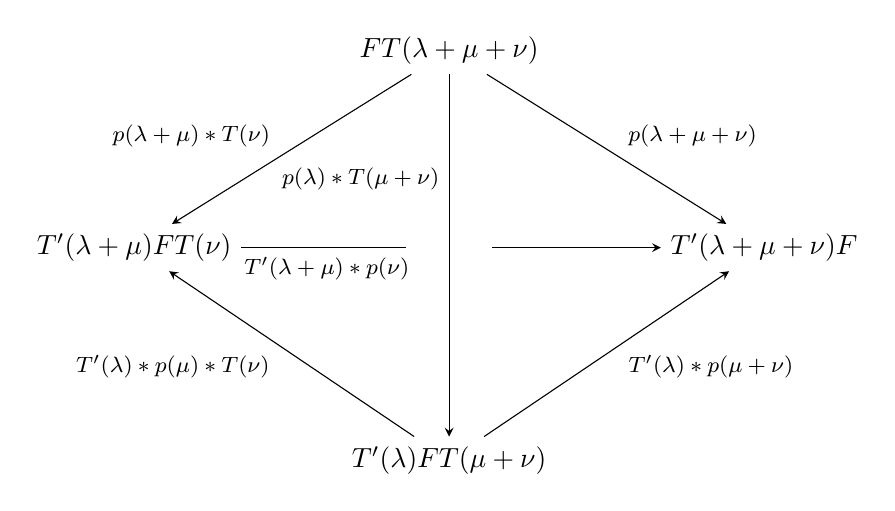
\begin{tikzpicture}[x=1cm,y=1cm,>=stealth]
    \node (a) at (0,3.2) {$FT(\lambda+\mu+\nu)$};
    \node (b) at (-4,0.7) {$T'(\lambda+\mu)FT(\nu)$};
    \node (c) at (4,0.7) {$T'(\lambda+\mu+\nu)F$};
    \node (d) at (0,-2.0) {$T'(\lambda)FT(\mu+\nu)$};
    \draw[->] (a) -- node[above left,pos=.55,font=\footnotesize]
      {$p(\lambda+\mu)*T(\nu)$} (b);
    \draw[->] (a) -- node[above right,pos=.55,font=\footnotesize]
      {$p(\lambda+\mu+\nu)$} (c);
    \draw[->] (a) -- node[left,pos=.29,font=\footnotesize]
      {$p(\lambda)*T(\mu+\nu)$} (d);
    \coordinate (bc-left) at (-0.55,0.7);
    \coordinate (bc-right) at (0.55,0.7);
    \draw (b) -- node[below,pos=.52,font=\footnotesize]
      {$T'(\lambda+\mu)*p(\nu)$} (bc-left);
    \draw[->] (bc-right) -- (c);
    \draw[->] (d) -- node[below left,pos=.55,font=\footnotesize]
      {$T'(\lambda)*p(\mu)*T(\nu)$} (b);
    \draw[->] (d) -- node[below right,pos=.55,font=\footnotesize]
      {$T'(\lambda)*p(\mu+\nu)$} (c);
  \end{tikzpicture}
\end{center}

\VerdierSemanticAnchor{ch1-1-5-5-faces}
この図式は四面体の形をしており、その四面はそれぞれ
$D(\lambda,\mu+\nu)$、$D(\lambda+\mu,\nu)$、
$D(\lambda,\mu)T(\nu)$、$T'(\lambda)D(\mu,\nu)$ である。
四つの場合を考え、余サイクル関係を用いれば (1.5.4.5) が得られる。

\VerdierSemanticAnchor{ch1-1-5-5-reduction}
一般の場合に導入すべき図式はもう少し複雑だが、恒等式 (1.2.1.3) を用いれば、
論証は上で概説したものに帰着する。(1.5.3.5) の証明には同じ図式で
\[
  \lambda=qe_1,\qquad \mu=q'e_1,\qquad \nu=q''e_1
\]
とおけばよい。

\VerdierSourcePageBlock{0056}%
\VerdierSemanticAnchor{ch1-1-5-6}
\noindent\textbf{図式 1.5.6.}\quad
次に主張 (1.5.4.3) を証明しよう。証明は次の図式に基づく。
簡単のため、遷移同型 $c,c'$ が恒等射である場合について書く：

\VerdierSemanticAnchor{ch1-1-5-7}
\noindent\textbf{1.5.7.}

\VerdierSemanticAnchor{ch1-1-5-7-diagram}
\begin{center}
  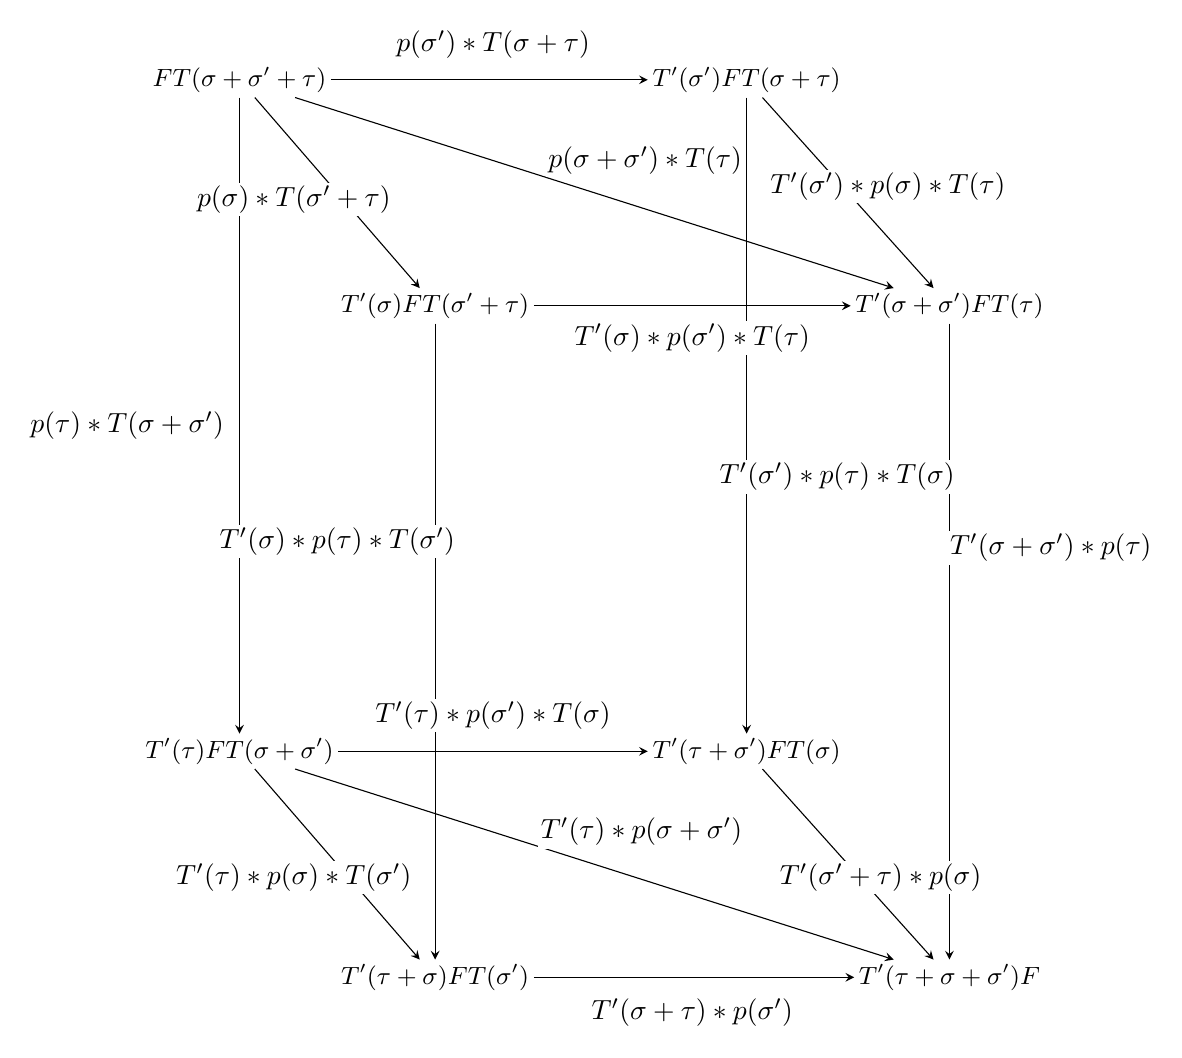
\begin{tikzpicture}[x=.92cm,y=.82cm,>=stealth,
      object/.style={inner sep=1.5pt,font=\small},
      lab/.style={font=\normalsize,fill=white,inner sep=1pt}]
    \node[object] (a) at (-5.8,13.0) {$FT(\sigma+\sigma'+\tau)$};
    \node[object] (b) at (1.2,13.0) {$T'(\sigma')FT(\sigma+\tau)$};
    \node[object] (c) at (-3.1,9.5) {$T'(\sigma)FT(\sigma'+\tau)$};
    \node[object] (d) at (4.0,9.5) {$T'(\sigma+\sigma')FT(\tau)$};
    \node[object] (e) at (-5.8,2.6) {$T'(\tau)FT(\sigma+\sigma')$};
    \node[object] (f) at (1.2,2.6) {$T'(\tau+\sigma')FT(\sigma)$};
    \node[object] (g) at (-3.1,-0.9) {$T'(\tau+\sigma)FT(\sigma')$};
    \node[object] (h) at (4.0,-0.9) {$T'(\tau+\sigma+\sigma')F$};

    \draw[->] (a) -- (b);
    \draw[->] (a) -- (c);
    \draw[->] (a) -- (d);
    \draw[->] (a) -- (e);
    \draw[->] (b) -- (d);
    \draw[->] (b) -- (f);
    \draw[->] (c) -- (d);
    \draw[->] (c) -- (g);
    \draw[->] (d) -- (h);
    \draw[->] (e) -- (f);
    \draw[->] (e) -- (g);
    \draw[->] (e) -- (h);
    \draw[->] (f) -- (h);
    \draw[->] (g) -- (h);

    \node[lab] at (-2.3,13.55) {$p(\sigma')*T(\sigma+\tau)$};
    \node[lab] at (-5.05,11.15) {$p(\sigma)*T(\sigma'+\tau)$};
    \node[lab] at (-0.2,11.75) {$p(\sigma+\sigma')*T(\tau)$};
    \node[lab] at (-7.35,7.65) {$p(\tau)*T(\sigma+\sigma')$};
    \node[lab] at (3.15,11.35) {$T'(\sigma')*p(\sigma)*T(\tau)$};
    \node[lab] at (2.45,6.85) {$T'(\sigma')*p(\tau)*T(\sigma)$};
    \node[lab] at (0.45,9.00) {$T'(\sigma)*p(\sigma')*T(\tau)$};
    \node[lab] at (-4.45,5.85) {$T'(\sigma)*p(\tau)*T(\sigma')$};
    \node[lab] at (5.40,5.75) {$T'(\sigma+\sigma')*p(\tau)$};
    \node[lab] at (-2.3,3.15) {$T'(\tau)*p(\sigma')*T(\sigma)$};
    \node[lab] at (-5.05,0.65) {$T'(\tau)*p(\sigma)*T(\sigma')$};
    \node[lab] at (-0.25,1.35) {$T'(\tau)*p(\sigma+\sigma')$};
    \node[lab] at (3.05,0.65) {$T'(\sigma'+\tau)*p(\sigma)$};
    \node[lab] at (0.45,-1.45) {$T'(\sigma+\tau)*p(\sigma')$};
  \end{tikzpicture}
\end{center}

\VerdierSemanticAnchor{ch1-1-5-7-delta-intro}
$\Delta(\sigma,\tau)$ を図式
$\textup{(1.5.4.2)}_{\sigma,\tau}$ とする。上の図式は%
\VerdierSourcePageContinue{0057}%
\VerdierSemanticAnchor{ch1-1-5-7-continuation}
五つの縦の図式を示している。それらは順に

\VerdierSemanticAnchor{ch1-1-5-7-vertical}
\[
  T'(\sigma')\Delta(\sigma,\tau),\quad
  T'(\sigma)\Delta(\sigma',\tau),\quad
  \Delta(\sigma,\tau)T(\sigma'),\quad
  \Delta(\sigma',\tau)T(\sigma),\quad
  \Delta(\sigma+\sigma',\tau)
\]
である。同様に四つの横の図式を示しており、それらは順に

\VerdierSemanticAnchor{ch1-1-5-7-horizontal}
\[
  D(\sigma,\sigma')T(\tau),\quad
  D(\sigma',\sigma)T(\tau),\quad
  T'(\tau)D(\sigma,\sigma'),\quad
  T'(\tau)D(\sigma',\sigma)
\]
である。

\VerdierSemanticAnchor{ch1-1-5-7-conclusion}
帰納法の仮定により、図式 $D(\sigma,\sigma')$ と
$D(\sigma',\sigma)$ はそれぞれ $\alpha(\sigma,\sigma')$-可換、
$\alpha(\sigma',\sigma)$-可換である。三つの場合を考えれば、主張
(1.5.4.3) の前半が従う。後半は $\sigma$ と $\tau$ の役割を入れ替えて
得られる。一般の場合に導入すべき図式はさらに複雑だが、恒等式
(1.2.1.3) を用いれば、論証は上で与えたものに帰着する。

\VerdierSemanticAnchor{ch1-1-5-8}
\noindent\textbf{注意 1.5.8.}\quad
命題 (1.5.2) は特に余サイクル $\alpha$ が自明な場合に適用できる。
このとき、圏 $\mathcal C'$ が加法圏でなくても、命題とその証明が
逐語的に拡張されることが分かる。

\VerdierSemanticAnchor{ch1-1-5-9}
\noindent\textbf{1.5.9.}\quad

\VerdierSemanticAnchor{ch1-1-5-9-functors}
\[
  (F_1,p_1),(F_2,p_2)\colon
  (\mathcal C,\mathbb Z^n,T,c)
  \longrightarrow
  (\mathcal C',\mathbb Z^n,T',c')
\]
を、それぞれ正規化された余サイクル
$\alpha_1,\alpha_2\in Z^2(\mathbb Z^n,\mathbb Z/2\mathbb Z)$
で捩られた二つの $\mathbb Z^n$-関手とする。また
$\beta\colon\mathbb Z^n\to\mathbb Z/2\mathbb Z$ を

\VerdierSemanticAnchor{ch1-1-5-9-eq1}
\begin{equation}
  \alpha_2(\sigma_1,\sigma_2)\alpha_1^{-1}(\sigma_1,\sigma_2)
  =\beta(\sigma_2)\beta(\sigma_1\sigma_2)^{-1}\beta(\sigma_1),
  \qquad \sigma_1,\sigma_2\in\mathbb Z^n,
  \tag{1.5.9.1}
\end{equation}
を満たす写像とし、$u\colon(F_1,p_1)\to(F_2,p_2)$ を関手の
$\beta$-射 (1.4.6) とする。$e_1,\ldots,e_n$ を $\mathbb Z^n$ の標準基底と
する。各 $i\in[1,n]$ に対し、次の図式は $\beta(e_i)$-可換である：

\VerdierSemanticAnchor{ch1-1-5-9-eq2}
\begin{equation}
  \mbox{%
    $\begin{tikzcd}[ampersand replacement=\&,column sep=6em,row sep=4em]
      F_1T(e_i)
        \arrow[r,"{p_1(e_i)}"]
        \arrow[d,"{u*T(e_i)}"']
        \& T'(e_i)F_1
          \arrow[d,"{T'(e_i)*u}"] \\
      F_2T(e_i)
        \arrow[r,"{p_2(e_i)}"]
        \& T'(e_i)F_2
    \end{tikzcd}$%
  }\;.
  \tag{1.5.9.2}
\end{equation}

\VerdierSourcePageBlock{0058}%
\VerdierSemanticAnchor{ch1-1-5-10-converse}
\noindent\textbf{逆に：}\par

\VerdierSemanticAnchor{ch1-1-5-10}
\VerdierSemanticAnchor{ch1-1-5-10-proposition}
\noindent\textbf{命題 1.5.10.}\quad
\emph{基礎となる関手の間の射 $u\colon F_1\to F_2$ で、各
$i\in[1,n]$ に対して図式 (1.5.9.2) が $\beta(e_i)$-可換であるものは、
関手の $\beta$-射である。}

\VerdierSemanticAnchor{ch1-1-5-10-proof}
実際、各 $\sigma\in\mathbb Z^n$ に対し、$R(\sigma)$ で次の性質を表す：

\VerdierSemanticAnchor{ch1-1-5-10-property}
\noindent\emph{$(R(\sigma))$\qquad 次の図式は $\beta(\sigma)$-可換である：}

\VerdierSemanticAnchor{ch1-1-5-10-eq1}
\begin{equation}
  \mbox{%
    $\begin{tikzcd}[ampersand replacement=\&,column sep=6em,row sep=4em]
      F_1T(\sigma)
        \arrow[r,"{p_1(\sigma)}"]
        \arrow[d,"{u*T(\sigma)}"']
        \& T'(\sigma)F_1
          \arrow[d,"{T'(\sigma)*u}"] \\
      F_2T(\sigma)
        \arrow[r,"{p_2(\sigma)}"]
        \& T'(\sigma)F_2
    \end{tikzcd}$%
  }\;.
  \tag*{\ensuremath{(1.5.10.1)_{\sigma}}}
\end{equation}

図式 $(1.5.10.1)_{\sigma_1}$、$(1.5.10.1)_{\sigma_2}$、
$(1.5.10.1)_{\sigma_1+\sigma_2}$ を調べれば、直ちに次が分かる：

\VerdierSemanticAnchor{ch1-1-5-10-closure}
\noindent\emph{性質 $R(\sigma_1)$、$R(\sigma_2)$、
$R(\sigma_1+\sigma_2)$ のうち二つが成り立てば、残る一つも成り立つ。}

\VerdierSemanticAnchor{ch1-1-5-10-conclusion}
さらに仮定により、性質 $R(e_i)$（$i\in[1,n]$）および $R(0)$ が
成り立つ。したがって $R(\sigma)$ はすべての
$\sigma\in\mathbb Z^n$ に対して成り立つ。

\VerdierSemanticAnchor{ch1-1-5-11}
\noindent\textbf{1.5.11.}\quad
厳密な $\mathbb Z^n$-圏とは、その自己同型群の中の $\mathbb Z^n$ の表現を
備えた圏である。このような表現を定めるには、互いに可換する $n$ 個の自己同型
$T(e_1),\ldots,T(e_n)$ を与えれば十分である。

\VerdierSemanticAnchor{ch1-1-5-12}
\noindent\textbf{1.5.12.}\quad
与えられた圏上の（必ずしも厳密でない）$\mathbb Z^n$-圏構造を決定する問題は、
はるかに簡単ではない。例えば、圏 $\mathcal C$ 上で、すべての
$\sigma\in\mathbb Z^n$ に対して
$T(\sigma)=\text{$\mathcal C$ の恒等関手}$ となる $\mathbb Z^n$-圏構造だけを
考える。このとき各対 $\sigma_1,\sigma_2\in\mathbb Z^n$ に対して、
$\mathcal C$ の恒等関手の自己同型群（これは可換群である）の元
$c(\sigma_1,\sigma_2)$ を与え、それらが恒等式 (1.2.1.3) を満たすことを
要求しなければならない。したがって、このような構造を与えることは、
$\mathcal C$ の恒等関手の自己同型群に値をとる $\mathbb Z^n$ 上の正規化された
非斉次 2-余サイクルを与えることである。さらに、二つのこのような構造が
$F=\text{$\mathcal C$ の恒等関手}$ を満たす $\mathbb Z^n$-関手 $(F,m)$ により
同型であるための必要十分条件は、対応する余サイクルが同じコホモロジー類に
属することである。

\VerdierSourcePageBlock{0059}%
\VerdierSemanticAnchor{ch1-1-5-13}
\noindent\textbf{1.5.13.}\quad
本書で用いる $\mathbb Z^n$-圏は厳密な圏である。したがって、(1.5.12) で
指摘した問題を一般の場合に扱うことはしない。しかし (1.5.12) の例は、
圏 $\mathcal C$ 上の $\mathbb Z$-圏構造の決定が特に簡単であることを示唆する。
実際その通りである。$E\text{-}\operatorname{Cat}$ を次の $U$-圏とする。
その対象は $U$ に属し、同値

\VerdierSemanticAnchor{ch1-1-5-13-eq1}
\begin{equation}
  T\colon\mathcal C\longrightarrow\mathcal C
  \tag{1.5.13.1}
\end{equation}
を備えた圏であり、その射は同型

\VerdierSemanticAnchor{ch1-1-5-13-eq2}
\begin{equation}
  m\colon FT\longrightarrow T'F
  \tag{1.5.13.2}
\end{equation}
を備えた関手 $F\colon\mathcal C\to\mathcal C'$ である。

すると $U$-圏 $\mathbb Z\text{-}\operatorname{Cat}$ から $U$-圏
$E\text{-}\operatorname{Cat}$ への関手

\VerdierSemanticAnchor{ch1-1-5-13-eq3}
\begin{equation}
  R\colon \mathbb Z\text{-}\operatorname{Cat}
  \longrightarrow E\text{-}\operatorname{Cat}
  \tag{1.5.13.3}
\end{equation}
が明らかに存在する。

\VerdierSemanticAnchor{ch1-1-5-13-action}
関手 $R$ は、$\mathbb Z$-圏 $(\mathcal C,\mathbb Z,T,c)$ に、同値
$T(1)\colon\mathcal C\to\mathcal C$ を備えた圏 $\mathcal C$ を対応させ、
各 $\mathbb Z$-関手
\[
  (F,m)\colon(\mathcal C,\mathbb Z,T,c)
  \longrightarrow(\mathcal C',\mathbb Z,T',c')
\]
に、同型 $m(1)\colon FT(1)\to T'(1)F$ を備えた関手 $F$ を対応させる。

\VerdierSemanticAnchor{ch1-1-5-14}
\VerdierSemanticAnchor{ch1-1-5-14-proposition}
\noindent\textbf{命題 1.5.14.}\quad
\emph{関手 $R$ は圏同値である。}

\VerdierSemanticAnchor{ch1-1-5-14-proof}
証明の指針だけを与える。命題 (1.5.2) と注意 (1.5.8) により $R$ は
充満忠実である。したがって、$R$ が本質的全射であることを示せばよい。
そこで、同値を備えた圏
$(\mathcal C,T\colon\mathcal C\to\mathcal C)$ をとる。
$T$ の擬逆関手 $T^{-1}\colon\mathcal C\to\mathcal C$ と、随伴同型

\VerdierSemanticAnchor{ch1-1-5-14-eq1}
\begin{equation}
  \begin{aligned}
    u&\colon\operatorname{id}_{\mathcal C}\longrightarrow TT^{-1},\\
    v&\colon\operatorname{id}_{\mathcal C}\longrightarrow T^{-1}T
  \end{aligned}
  \tag{1.5.14.1}
\end{equation}
をとる。

各整数 $n>0$ について、関手 $T^n$ と $(T^{-1})^n$ は互いに随伴である。
したがって随伴同型

\VerdierSemanticAnchor{ch1-1-5-14-eq2}
\begin{equation}
  \begin{aligned}
    u^{(n)}&\colon\operatorname{id}_{\mathcal C}
      \longrightarrow T^n(T^{-1})^n,\\
    v^{(n)}&\colon\operatorname{id}_{\mathcal C}
      \longrightarrow (T^{-1})^nT^n
  \end{aligned}
  \tag{1.5.14.2}
\end{equation}
が得られる。%
\VerdierSourcePageContinue{0060}%
\VerdierSemanticAnchor{ch1-1-5-14-continuation}
そこで、次のようにおく：

\VerdierSemanticAnchor{ch1-1-5-14-eq3}
\begin{equation}
  \begin{aligned}
    T(0)&=\operatorname{id}_{\mathcal C},\\
    T(n)&=T^n, && n>0,\\
    T(n)&=(T^{-1})^{-n}, && n<0.
  \end{aligned}
  \tag{1.5.14.3}
\end{equation}

\VerdierSemanticAnchor{ch1-1-5-14-cocycle-data}
さらに、整数の各対 $(n,n')$ に対し、同型
\[
  c(n',n)\colon T(n+n')\longrightarrow T(n)T(n')
\]
を次のように定める：

\VerdierSemanticAnchor{ch1-1-5-14-eq4}
\begin{equation}
  \begin{aligned}
    n,n'&\geq 0,
      &c(n',n)&=\operatorname{id},\\
    n,n'&\leq 0,
      &c(n',n)&=\operatorname{id},\\
    n'&\leq 0, n\geq 0, n+n'\leq 0,
      &c(n',n)&=u^{(n)}\mathbin{*}T(n+n'),\\
    n'&\leq 0, n\geq 0, n+n'\geq 0,
      &c(n',n)&=T(n+n')\mathbin{*}u^{(-n')},\\
    n'&\geq 0, n\leq 0, n+n'\leq 0,
      &c(n',n)&=T(n+n')\mathbin{*}v^{(n')},\\
    n'&\geq 0, n\leq 0, n+n'\geq 0,
      &c(n',n)&=v^{(-n)}\mathbin{*}T(n+n').
  \end{aligned}
  \tag{1.5.14.4}
\end{equation}

\VerdierSemanticAnchor{ch1-1-5-14-conclusion}
これによって実際に $\mathbb Z$-圏が定義されたことを確かめるには、
(1.2.1.3) 型の恒等式が成り立つことを検証すればよい。この検証は射
$u^{(n)}$ と $v^{(n)}$ が満たす古典的な恒等式に基づく。詳細は読者に委ねる。

\VerdierSemanticAnchor{ch1-1-6}
\subsection{Koszul 余サイクルと符号規則}

\VerdierSemanticAnchor{ch1-1-6-1}
\noindent\textbf{1.6.1.}\quad
$e_1,\ldots,e_n$ を $\mathbb Z^n$ の基底とする。
$i,j\in[1,n]$、$i\neq j$ に対し、$\mathbb Z^n_{i,j}$ を $e_i$ と
$e_j$ が生成する $\mathbb Z^n$ の部分群とする。制限準同型は準同型

\VerdierSemanticAnchor{ch1-1-6-1-eq1}
\begin{equation}
  H^2(\mathbb Z^n,\mathbb Z/2\mathbb Z)
  \longrightarrow
  \bigoplus_{\substack{i,j\in[1,n]\\ i<j}}
    H^2(\mathbb Z^n_{i,j},\mathbb Z/2\mathbb Z)
  \tag{1.6.1.1}
\end{equation}
を定める。

（標準的な）同型

\VerdierSemanticAnchor{ch1-1-6-1-eq2}
\begin{equation}
  H^2(\mathbb Z^n_{i,j},\mathbb Z/2\mathbb Z)
  \simeq \mathbb Z/2\mathbb Z
  \tag{1.6.1.2}
\end{equation}
がある。

\VerdierSemanticAnchor{ch1-1-6-1-conclusion}
準同型 (1.6.1.1) は同型である。

\VerdierSourcePageBlock{0061}%
\VerdierSemanticAnchor{ch1-1-6-2}
\VerdierSemanticAnchor{ch1-1-6-2-proposition}
\noindent\textbf{命題 1.6.2.}\quad

\VerdierSemanticAnchor{ch1-1-6-2-part1}
\noindent\emph{1) $\alpha\in Z^2(\mathbb Z^n,\mathbb Z/2\mathbb Z)$ を
正規化された非斉次余サイクル、
$\dot\alpha\in H^2(\mathbb Z^n,\mathbb Z/2\mathbb Z)$ をその
コホモロジー類、
$\dot\alpha_{i,j}\in H^2(\mathbb Z^n_{i,j},\mathbb Z/2\mathbb Z)$ を
その成分とする。このとき（(1.6.1.2) を用いて）：}

\VerdierSemanticAnchor{ch1-1-6-2-eq1}
\begin{equation}
  \dot\alpha_{i,j}
  =\alpha(e_i,e_j)^{-1}\alpha(e_j,e_i).
  \tag{1.6.2.1}
\end{equation}

\VerdierSemanticAnchor{ch1-1-6-2-convention}
\noindent\emph{（$\mathbb Z/2\mathbb Z$ の群演算は乗法的に記す。）}

\VerdierSemanticAnchor{ch1-1-6-2-part2}
\noindent\emph{2) $\alpha_1$ と $\alpha_2$ を
$Z^2(\mathbb Z^n,\mathbb Z/2\mathbb Z)$ のコホモロガスな二元とし、各
$i\in[1,n]$ に対して $\beta_i\in\mathbb Z/2\mathbb Z$ をとる。このとき、
写像}

\VerdierSemanticAnchor{ch1-1-6-2-beta-map}
\begin{equation*}
  \beta\colon\mathbb Z^n\longrightarrow\mathbb Z/2\mathbb Z
\end{equation*}
\noindent\emph{で次を満たすものがただ一つ存在する：}

\VerdierSemanticAnchor{ch1-1-6-2-eq2}
\begin{equation}
  \begin{aligned}
    \alpha_2(\sigma_1,\sigma_2)\alpha_1^{-1}(\sigma_1,\sigma_2)
      &=\beta(\sigma_2)\beta(\sigma_1+\sigma_2)^{-1}\beta(\sigma_1),\\[-1mm]
    &\hspace{7em}\text{ただし }\sigma_1,\sigma_2\in\mathbb Z^n,
  \end{aligned}
  \tag{1.6.2.2}
\end{equation}

\VerdierSemanticAnchor{ch1-1-6-2-eq3}
\begin{equation}
  \beta(e_i)=\beta_i.
  \tag{1.6.2.3}
\end{equation}

\VerdierSemanticAnchor{ch1-1-6-2-proof}
\VerdierSemanticAnchor{ch1-1-6-2-proof-first}
第1の主張を証明するため $n=2$ の場合に帰着し、$\alpha$ を余境界で変更しても
$\alpha(e_i,e_j)^{-1}\alpha(e_j,e_i)$ が変わらないことを直ちに確かめる。
$\alpha$ が余境界ならば対称であり、したがって公式 (1.6.2.1) はこの場合に
成り立つ。一方、余サイクル

\VerdierSemanticAnchor{ch1-1-6-2-alpha0}
\begin{equation*}
  \alpha_0(p_1e_i+q_1e_j,p_2e_i+q_2e_j)=(-1)^{q_1p_2}
\end{equation*}
は $0$ とコホモロガスではない。実際、

\VerdierSemanticAnchor{ch1-1-6-2-alpha0-test}
\begin{equation*}
  \alpha_0(e_i,e_j)^{-1}\alpha_0(e_j,e_i)=-1
\end{equation*}
であり、零とコホモロガスでない任意の余サイクルは $\alpha_0$ と
コホモロガスである。

\VerdierSemanticAnchor{ch1-1-6-2-proof-second}
第2の主張については、(1.6.2.2) の二つの解の比が群準同型であることに注意
する。したがって (1.6.2.2) の解は、各 $e_i$ 上で指定した値をとるように、
ただ一つの群準同型によって常に修正できる。

\VerdierSemanticAnchor{ch1-1-6-3}
\VerdierSemanticAnchor{ch1-1-6-3-definition}
\noindent\textbf{定義 1.6.3.}\quad
$e_1,\ldots,e_n$ を $\mathbb Z^n$ の基底とする。\emph{基底
$e_1,\ldots,e_n$ に関する Koszul 類}とは、各群
$H^2(\mathbb Z^n_{i,j},\mathbb Z/2\mathbb Z)$ への制限が非零である
$H^2(\mathbb Z^n,\mathbb Z/2\mathbb Z)$ のただ一つの元である。

\VerdierSemanticAnchor{ch1-1-6-3-basis-dependence}
Koszul 類の定義は $\mathbb Z^n$ の基底の選択に依存することに注意する。
一般には、異なる二つの基底に付随する Koszul 類は異なる。

\VerdierSemanticAnchor{ch1-1-6-3-filtration}
$e_1,\ldots,e_n$ を $[1,n]$ の自然順序に従って並べた $\mathbb Z^n$ の
基底とする。$j\leq i$ を満たす $e_j$ が生成する部分群を
$\mathbb Z^n(\leq i)$ と記し、$j\geq i$ を満たす $e_j$ が生成する部分群を
$\mathbb Z^n(\geq i)$ と記す。

\VerdierSourcePageBlock{0062}%
\VerdierSemanticAnchor{ch1-1-6-4}
\VerdierSemanticAnchor{ch1-1-6-4-definition}
\noindent\textbf{定義 1.6.4.}\quad
\emph{$\mathbb Z^n$ の順序付き基底 $e_1,\ldots,e_n$ に関する Koszul
余サイクル}とは、基底 $e_1,\ldots,e_n$ に関する Koszul 類に属し、次を
満たすただ一つの余サイクル $\alpha$ である：

\VerdierSemanticAnchor{ch1-1-6-4-eq1}
\begin{equation}
  \alpha(\sigma_1,\sigma_2)=1
  \quad
  \forall\sigma_1\in\mathbb Z^n(\leq i),\quad
  \forall\sigma_2\in\mathbb Z^n(\geq i),\quad
  \forall i\in[1,n].
  \tag{1.6.4.1}
\end{equation}

\VerdierSemanticAnchor{ch1-1-6-4-coordinate-intro}
$\sigma_1=\sum_{i=1}^{n}p_i e_i$ および
$\sigma_2=\sum_{i=1}^{n}q_i e_i$ を $\mathbb Z^n$ の二元とすると、

\VerdierSemanticAnchor{ch1-1-6-4-eq2}
\begin{equation}
  \alpha(\sigma_1,\sigma_2)
  =(-1)^{\left(\sum_{i<j}q_i p_j\right)}.
  \tag{1.6.4.2}
\end{equation}

\VerdierSemanticAnchor{ch1-1-6-4-justification}
この定義には説明が必要である。(1.6.4.1) を満たす Koszul 類の余サイクルの
存在は明らかである。実際、直ちに計算すれば、余サイクル (1.6.4.2) は
(1.6.4.1) を満たし、Koszul 類に属することが分かる (1.6.2)。一意性を
確かめるには、$\alpha$ とコホモロガスな任意の余サイクルが

\VerdierSemanticAnchor{ch1-1-6-4-cohomologous-form}
\begin{equation*}
  \alpha_1(\sigma_1,\sigma_2)
  =\alpha(\sigma_1,\sigma_2)
   \beta(\sigma_2)\beta(\sigma_1+\sigma_2)^{-1}\beta(\sigma_1)
\end{equation*}
の形であり、この余サイクルが (1.6.4.1) を満たすことと

\VerdierSemanticAnchor{ch1-1-6-4-condition}
\begin{equation*}
  \beta(\sigma_1+\sigma_2)=\beta(\sigma_1)\beta(\sigma_2)
  \quad
  \forall i,\quad
  \forall\sigma_1\in\mathbb Z^n(\leq i),\quad
  \forall\sigma_2\in\mathbb Z^n(\geq i)
\end{equation*}
が同値であることに注意すればよい。

\VerdierSemanticAnchor{ch1-1-6-4-uniqueness}
ここから $\beta\colon\mathbb Z^n\to\mathbb Z/2\mathbb Z$ が群準同型である
ことが直ちに従い、したがって $\alpha_1=\alpha$ である。

\VerdierSemanticAnchor{ch1-1-6-5}
\VerdierSemanticAnchor{ch1-1-6-5-order-dependence}
\noindent\textbf{1.6.5.}\quad
Koszul 余サイクルの定義は、$\mathbb Z^n$ の基底 $e_1,\ldots,e_n$ に
入れた全順序に本質的に依存する。$[1,n]$ 上の自然順序を $\leq$、任意の
全順序を $\leq_s$ とする。$s$ を次を満たす $[1,n]$ のただ一つの置換とする：

\VerdierSemanticAnchor{ch1-1-6-5-eq1}
\begin{equation}
  i\leq_s j\quad\Longleftrightarrow\quad s(i)\leq s(j).
  \tag{1.6.5.1}
\end{equation}

\VerdierSemanticAnchor{ch1-1-6-5-cocycles}
$\alpha$ と $\alpha_s$ を、それぞれ順序 $\leq$ と $\leq_s$ に関する
Koszul 余サイクルとする。このとき

\VerdierSemanticAnchor{ch1-1-6-5-eq2}
\VerdierSemanticAnchor{ch1-1-6-5-eq2-natural}
\VerdierSemanticAnchor{ch1-1-6-5-eq2-coordinates}
\VerdierSemanticAnchor{ch1-1-6-5-eq2-permuted}
\begin{equation}
  \begin{aligned}
    \alpha(\sigma_1,\sigma_2)
      &=(-1)^{\left(\sum_{i<j}q_i p_j\right)},\\
    \sigma_1&=\sum_i p_i e_i,
      \qquad \sigma_2=\sum_i q_i e_i,\\
    \alpha_s(\sigma_1,\sigma_2)
      &=(-1)^{\left(\sum_{s(i)<s(j)}q_i p_j\right)},
  \end{aligned}
  \tag{1.6.5.2}
\end{equation}
\VerdierSemanticAnchor{ch1-1-6-5-open}%
\VerdierSourcePageContinue{0063}%
\VerdierSemanticAnchor{ch1-1-6-5-continuation}
ここから直ちに

\VerdierSemanticAnchor{ch1-1-6-5-deduction}
\VerdierSemanticAnchor{ch1-1-6-5-beta-s-coboundary}
\begin{equation*}
  \alpha_s(\sigma_1,\sigma_2)\alpha(\sigma_1,\sigma_2)^{-1}
  =\beta_s(\sigma_2)\beta_s(\sigma_1+\sigma_2)^{-1}\beta_s(\sigma_1)
\end{equation*}
が従う。ただし

\VerdierSemanticAnchor{ch1-1-6-5-eq3}
\VerdierSemanticAnchor{ch1-1-6-5-eq3-beta}
\VerdierSemanticAnchor{ch1-1-6-5-eq3-basis}
\begin{equation}
  \begin{aligned}
    \beta_s(\sigma_1)
      &=(-1)^{\left(
          \sum_{\substack{i<j\\s(i)>s(j)}}p_i p_j
        \right)},\\
    \beta_s(e_i)&=1,
      \qquad \forall i\in[1,n].
  \end{aligned}
  \tag{1.6.5.3}
\end{equation}

\VerdierSemanticAnchor{ch1-1-6-5-application}
したがって (1.6.2) により、次を満たす任意の写像
$\beta\colon\mathbb Z^n\to\mathbb Z/2\mathbb Z$

\VerdierSemanticAnchor{ch1-1-6-5-eq4}
\begin{equation}
  \alpha_s(\sigma_1,\sigma_2)\alpha(\sigma_1,\sigma_2)^{-1}
  =\beta(\sigma_2)\beta(\sigma_1+\sigma_2)^{-1}\beta(\sigma_1)
  \tag{1.6.5.4}
\end{equation}

\VerdierSemanticAnchor{ch1-1-6-5-eq5-intro}
は

\VerdierSemanticAnchor{ch1-1-6-5-eq5}
\begin{equation}
  \beta=\beta_s\eta
  \tag{1.6.5.5}
\end{equation}
の形である。

\VerdierSemanticAnchor{ch1-1-6-5-closure}
ここで $\eta\colon\mathbb Z^n\to\mathbb Z/2\mathbb Z$ は
$e_j\in\mathbb Z^n$ 上で $\beta(e_j)$ の値をとるただ一つの群準同型である。

\VerdierSemanticAnchor{ch1-1-6-6}
\VerdierSemanticAnchor{ch1-1-6-6-product-setup}
\noindent\textbf{1.6.6.}\quad
$(C_i,\mathbb Z,T_i,c_i)$、$1\leq i\leq n$ を $\mathbb Z$-圏とし、
$(D,\mathbb Z,T,c)$ を加法的な $\mathbb Z$-圏とする。
$(C,\mathbb Z^n,T,c)$ を $(C_i,\mathbb Z,T_i,c_i)$ の積圏とする。
群 $\mathbb Z^n$ には順序付き基底 $e_1,\ldots,e_n$ が自然に備わる。
これは次の公式によって同型を除いて $C$ に作用する（ここでは (1.3.12) で
導入した右側の記法を用いる）：

\VerdierSemanticAnchor{ch1-1-6-6-eq1}
\begin{equation}
  (X_1,\ldots,X_n)[\sigma]
  =(X_1[l_1],\ldots,X_n[l_n]),
  \qquad
  \sigma=\sum_{i=1}^{n}l_i e_i.
  \tag{1.6.6.1}
\end{equation}

\VerdierSemanticAnchor{ch1-1-6-6-phi-action}
$\varphi\colon\mathbb Z^n\to\mathbb Z$ を
$\varphi(\sum_{i=1}^{n}l_i e_i)=\sum_{i=1}^{n}l_i$ で定まる準同型とする。
$\mathbb Z^n$ を $\varphi$ を通じて $D$ に作用させる (1.4.1)。この状況では
常に次の規約を用いる：

\VerdierSemanticAnchor{ch1-1-6-6-sign-rule-1}
\noindent\textbf{符号規則 I：}
\emph{明示的に別の指定がない限り、$C$ から $D$ への関手は常に順序付き基底
$e_1,\ldots,e_n$ に関する Koszul 余サイクルで捩られた
$\mathbb Z^n$-関手とする。}

\VerdierSemanticAnchor{ch1-1-6-6-sign-rule-2}
\noindent\textbf{符号規則 II：}
\emph{明示的に別の指定がない限り、関手の射は常に自明な準同型
$\beta\colon\mathbb Z^n\to\mathbb Z/2\mathbb Z$ に関する
$\mathbb Z^n$-関手の射とする (1.4.6)。}

\VerdierSourcePageBlock{0064}%
\VerdierSemanticAnchor{ch1-1-6-6-functor-characterization}
命題 (1.5.2) により、$C$ から $D$ への関手を指定することは、関手

\VerdierSemanticAnchor{ch1-1-6-6-eq2}
\begin{equation}
  (X_1,\ldots,X_n)\longmapsto F(X_1,\ldots,X_n)
  \tag{1.6.6.2}
\end{equation}

\VerdierSemanticAnchor{ch1-1-6-6-transition-isomorphisms}
と関手の同型

\VerdierSemanticAnchor{ch1-1-6-6-eq3}
\begin{equation}
  p_i\colon
  F(X_1,\ldots,X_i[1],\ldots,X_n)
  \xrightarrow{\ \sim\ }
  F(X_1,\ldots,X_n)[1]
  \tag{1.6.6.3}
\end{equation}

\VerdierSemanticAnchor{ch1-1-6-6-anticommutativity}
を指定し、図式 (1.5.1.2)

\VerdierSemanticAnchor{ch1-1-6-6-anticommutativity-diagram}
\begin{equation*}
  \mbox{%
    $\begin{tikzcd}[ampersand replacement=\&,column sep=2.8em,row sep=3.8em]
      F(X_1,\ldots,X_i[1],\ldots,X_j[1],\ldots,X_n)
        \arrow[r,"{p_i}"]
        \arrow[d,"{p_j}"]
        \& F(X_1,\ldots,X_i,\ldots,X_j[1],\ldots,X_n)[1]
          \arrow[d,"{p_j[1]}"] \\
      F(X_1,\ldots,X_i[1],\ldots,X_j,\ldots,X_n)[1]
        \arrow[r,"{p_i[1]}"]
        \& F(X_1,\ldots,X_i,\ldots,X_j,\ldots,X_n)[2]
    \end{tikzcd}$%
  }
\end{equation*}

が $i<j$ に対して反可換となるようにすることに等しい。（図式 (1.5.1.2) を
簡単にするため、$D$ の遷移同型を恒等射と仮定した。本書では常にそうである。）

\VerdierSemanticAnchor{ch1-1-6-6-morphism-characterization}
同様に命題 (1.5.10) により、ここで考える関手の射
$u\colon F\to F'$ は次の条件に従う。すなわち下の図式は可換である：

\VerdierSemanticAnchor{ch1-1-6-6-eq4}
\begin{equation}
  \mbox{%
    $\begin{tikzcd}[ampersand replacement=\&,column sep=5.0em,row sep=3.8em]
      F(X_1,\ldots,X_i[1],\ldots,X_n)
        \arrow[r,"u"]
        \arrow[d,"{p_i}"]
        \& F'(X_1,\ldots,X_i[1],\ldots,X_n)
          \arrow[d,"{p'_i}"] \\
      F(X_1,\ldots,X_i,\ldots,X_n)[1]
        \arrow[r,"{u[1]}"]
        \& F'(X_1,\ldots,X_i,\ldots,X_n)[1]
    \end{tikzcd}$%
  }
  \tag{1.6.6.4}
\end{equation}

\VerdierSemanticAnchor{ch1-1-6-6-underlying-convention}
文脈上混同のおそれがないとき、$\mathbb Z$-圏をその基礎圏で表し、捩られた
$\mathbb Z^n$-関手をその基礎関手で表す。

\VerdierSourcePageSilent{0065}%

\clearpage
\VerdierSourcePageBlock{0066}%
\VerdierSemanticAnchor{ch1-2}
\section{加法圏における複体}

\VerdierSemanticAnchor{ch1-2-1}
\subsection{\texorpdfstring{$n$}{n}-重複複体}

\VerdierSemanticAnchor{ch1-2-1-1}
\noindent\textbf{2.1.1.}\quad
まず記法を定める。集合

\VerdierSemanticAnchor{ch1-2-1-1-set}
\begin{equation*}
  [n]=\{p\in\mathbb Z\mid 1\leq p\leq n\}
\end{equation*}
を $[n]$ と記す。

\VerdierSemanticAnchor{ch1-2-1-1-free-group}
集合 $[n]$ が生成する自由アーベル群を $\mathbb Z[n]$ と記し、各
$i\in[n]$ に対して、$i$ に対応する $\mathbb Z[n]$ の生成元を $e_i$ と
記す。写像 $\varphi\colon[n]\to[m]$ に対し、対応する群準同型
$\mathbb Z[n]\to\mathbb Z[m]$ も $\varphi$ と記す。この節では $C$ を
加法圏とする。

\VerdierSemanticAnchor{ch1-2-1-2}
\VerdierSemanticAnchor{ch1-2-1-2-definition}
\noindent\textbf{定義 2.1.2.}\quad
$C$ の対象からなる\emph{$n$-重複複体}とは、次のデータからなる対象である：

\begin{enumerate}
\renewcommand{\labelenumi}{\arabic{enumi})}
\item \VerdierSemanticAnchor{ch1-2-1-2-objects}%
  各 $\sigma\in\mathbb Z[n]$ に対して $C$ の対象 $X^\sigma$；
\item \VerdierSemanticAnchor{ch1-2-1-2-differentials}%
  各 $\sigma\in\mathbb Z[n]$ と各 $i\in[n]$ に対して射
  \VerdierSemanticAnchor{ch1-2-1-2-differential-map}%
  \begin{equation*}
    d^{\sigma,i}\colon X^\sigma\longrightarrow X^{\sigma+e_i},
  \end{equation*}
  ただし、これらの射は次の条件に従う：
\end{enumerate}

\VerdierSemanticAnchor{ch1-2-1-2-eq1}
\begin{equation}
  \begin{aligned}
    d^{\sigma+e_i,i}d^{\sigma,i}&=0
      &&\forall\sigma\in\mathbb Z[n],\ \forall i\in[n],\\
    d^{\sigma+e_j,i}d^{\sigma,j}
      &=d^{\sigma+e_i,j}d^{\sigma,i}
      &&\forall\sigma\in\mathbb Z[n],\ \forall i,j\in[n].
  \end{aligned}
  \tag{2.1.2.1}
\end{equation}

\VerdierSemanticAnchor{ch1-2-1-3}
\noindent\textbf{2.1.3.}\quad
$C$ の対象からなる $n$-重複複体を、通常は単に $C$ における
\emph{$n$-重複複体}と呼ぶ。$(X^\sigma,d^{\sigma,i})$ を $C$ における
$n$-重複複体とする。
\VerdierSemanticAnchor{ch1-2-1-3-component}
対象 $X^\sigma$ を複体 $(X^\sigma,d^{\sigma,i})$ の
\emph{次数 $\sigma$ の成分}と呼ぶ。
\VerdierSemanticAnchor{ch1-2-1-3-differential}
射 $d^{\sigma,i}$ を複体 $(X^\sigma,d^{\sigma,i})$ の
\emph{方向 $i$ における次数 $\sigma$ の微分}と呼ぶ。
\VerdierSemanticAnchor{ch1-2-1-3-notation}
$Y$ を $C$ における $n$-重複複体とする。$Y$ の次数 $\sigma$ の成分を
$Y^\sigma$、方向 $i$ における次数 $\sigma$ の微分を $d_Y^{\sigma,i}$ と
記す。

\VerdierSemanticAnchor{ch1-2-1-4}
\VerdierSemanticAnchor{ch1-2-1-4-definition}
\noindent\textbf{定義 2.1.4.}\quad
$Y$ と $Y'$ を $C$ における二つの $n$-重複複体とする。$Y$ から $Y'$ への
\emph{複体の射}とは、微分と可換する $C$ の射の族

\VerdierSemanticAnchor{ch1-2-1-4-family}
\begin{equation*}
  \bigl(f^\sigma\colon Y^\sigma\longrightarrow Y'^{\sigma}\bigr)_{
    \sigma\in\mathbb Z[n]}
\end{equation*}
すなわち次を満たす族である：

\VerdierSemanticAnchor{ch1-2-1-4-eq1}
\begin{equation}
  f^{\sigma+e_i}d_Y^{\sigma,i}
  =d_{Y'}^{\sigma,i}f^\sigma.
  \tag{2.1.4.1}
\end{equation}

\VerdierSourcePageBlock{0067}%
\VerdierSemanticAnchor{ch1-2-1-5}
\noindent\textbf{2.1.5.}\quad
射 $f^\sigma\colon Y^\sigma\to Y'^\sigma$ を射 $(f^\sigma)$ の
\emph{次数 $\sigma$ の成分}と呼ぶ。$f\colon Y\to Y'$ を $n$-重複複体の
射とするとき、$f$ の次数 $\sigma$ の成分を $f^\sigma$ と記す。
\VerdierSemanticAnchor{ch1-2-1-5-composition}
$n$-重複複体の射は明らかな仕方で、成分ごとに合成される。
\VerdierSemanticAnchor{ch1-2-1-5-category}
$C$ の対象からなる $n$-重複複体は、$\operatorname{comp}^{n}(C)$ と記す
圏をなす。$n=1$ のときは簡略記法
$\operatorname{comp}^{1}(C)=\operatorname{comp}(C)$ を用いる。
$\operatorname{comp}(C)$ の対象を $C$ における\emph{単純複体}、また混同の
おそれがなければ単に $C$ における\emph{複体}と呼ぶ。圏
$\operatorname{comp}^{n}(C)$ は加法圏である。

\VerdierSemanticAnchor{ch1-2-1-6}
\noindent\textbf{2.1.6.}\quad
$Y$ を $C$ における $n$-重複複体とする。$Y$ の次数 $\sigma$ の成分を
$Y_{-\sigma}$、方向 $i$ における次数 $\sigma$ の微分を
$d^Y_{-\sigma,i}$ と記すこともある。
\VerdierSemanticAnchor{ch1-2-1-6-positive-finite}
この記法は、とくに $Y$ が単純複体で、正の次数の成分が有限個を除いて
消える場合に用いる。同様に、$f\colon Y\to Y'$ を $n$-重複複体の射と
すると、射 $f$ の次数 $\sigma$ の成分を $f_{-\sigma}$ と記すことがある。

\VerdierSemanticAnchor{ch1-2-1-7}
\noindent\textbf{2.1.7.}\quad
$\varphi\colon[n]\to[m]$ を写像とする。
\VerdierSemanticAnchor{ch1-2-1-7-summable}
各 $\tau\in\mathbb Z[m]$ に対して、$\varphi(\sigma)=\tau$ かつ
$Y^\sigma\neq0$ となる $\sigma\in\mathbb Z[n]$ が有限個しかないとき、
$C$ における $n$-重複複体 $Y$ を\emph{$\varphi$-総和可能}という。
$\varphi$ が唯一の写像 $[n]\to[1]$ であるときは、単に\emph{総和可能}という。
\VerdierSemanticAnchor{ch1-2-1-7-composition}
$[n]\xrightarrow{\varphi}[m]\xrightarrow{\psi}[p]$ を二つの写像とする。
$\psi\varphi$-総和可能な任意の $n$-重複複体 $Y$ は $\varphi$-総和可能でも
ある。とくに、総和可能な任意の $n$-重複複体は、任意の写像
$[n]\xrightarrow{\varphi}[m]$ に対して $\varphi$-総和可能である。
\VerdierSemanticAnchor{ch1-2-1-7-injective}
$\varphi$ が単射ならば、すべての複体は $\varphi$-総和可能である。
\VerdierSemanticAnchor{ch1-2-1-7-category}
\emph{$\varphi$-総和可能な $n$-重複複体の圏}とは、
$\varphi$-総和可能な複体によって定まる $\operatorname{comp}^{n}(C)$ の
充満部分圏である。

\VerdierSemanticAnchor{ch1-2-2}
\subsection{付随する単純複体}

\VerdierSemanticAnchor{ch1-2-2-1}
\noindent\textbf{2.2.1.}\quad
各 $\sigma\in\mathbb Z[n]$ を
$\sigma=\sum_{j\in[n]}l_je_j$、$l_j\in\mathbb Z$ と書き、各
$i\in[n]$ に対して

\VerdierSemanticAnchor{ch1-2-2-1-eq1}
\begin{equation}
  \varepsilon(\sigma,i)=(-1)^{\left(\sum_{j<i}l_j\right)}
  \tag{2.2.1.1}
\end{equation}
とおく。

\VerdierSemanticAnchor{ch1-2-2-1-sign-map}
公式 (2.2.1.1) は $\mathbb Z[n]\times[n]$ から符号群 $\{-1,1\}$ への写像
\begin{equation*}
  (\sigma,i)\longmapsto\varepsilon(\sigma,i)
\end{equation*}
を定める。各 $i\in[n]$ について
$\sigma\longmapsto\varepsilon(\sigma,i)$ が群準同型であり、%
\VerdierSourcePageContinue{0068}%
\VerdierSemanticAnchor{ch1-2-2-1-continuation}%
$j<i$ ならば $\varepsilon(e_j,i)=-1$、$i\leq j$ ならば
$\varepsilon(e_j,i)=1$ であることが直ちに分かる。さらに、写像
$(\sigma,i)\mapsto\varepsilon(\sigma,i)$ はこれらの性質によって一意に
定まる。ここから関係式

\VerdierSemanticAnchor{ch1-2-2-1-eq2}
\begin{equation}
  \varepsilon(\sigma,i)\varepsilon(\sigma+e_i,j)
  =-\varepsilon(\sigma,j)\varepsilon(\sigma+e_j,i)
  \tag{2.2.1.2}
\end{equation}
が直ちに従う。これは各 $\sigma\in\mathbb Z[n]$ および
$(i,j)\in[n]\times[n]$、$i\neq j$ に対して成り立つ。

\VerdierSemanticAnchor{ch1-2-2-2}
\noindent\textbf{2.2.2.}\quad
$Y$ を $C$ における $n$-重複複体とする。次のようにおく：

\VerdierSemanticAnchor{ch1-2-2-2-eq1}
\begin{equation}
  \delta_Y^{\sigma,i}=\varepsilon(\sigma,i)d_Y^{\sigma,i}.
  \tag{2.2.2.1}
\end{equation}

\VerdierSemanticAnchor{ch1-2-2-2-eq2}
(2.2.1.2) から、関係式 (2.1.2.1) は次の関係式と同値である：
\begin{equation}
  \begin{aligned}
    \delta_Y^{\sigma+e_i,i}\delta_Y^{\sigma,i}
      &=0,
      &&\forall\sigma\in\mathbb Z[n],\quad\forall i\in[n],\\
    \delta_Y^{\sigma+e_j,i}\delta_Y^{\sigma,j}
      +\delta_Y^{\sigma+e_i,j}\delta_Y^{\sigma,i}
      &=0,
      &&\forall\sigma\in\mathbb Z[n],\quad\forall i,j\in[n].
  \end{aligned}
  \tag{2.2.2.2}
\end{equation}

\VerdierSemanticAnchor{ch1-2-2-2-pushforward}
ここで $\varphi\colon[n]\to[m]$ を写像とし、$Y$ が
$\varphi$-総和可能であるとする。次の公式によって $m$-重複複体
$\int_\varphi Y$ を定める：

\VerdierSemanticAnchor{ch1-2-2-2-eq3}
\begin{equation}
  \left(\int_\varphi Y\right)^\tau
  =\bigoplus_{\varphi(\sigma)=\tau}Y^\sigma,
  \qquad \forall\tau\in\mathbb Z[m],
  \tag{2.2.2.3}
\end{equation}

\VerdierSemanticAnchor{ch1-2-2-2-eq4}
\begin{equation}
  \begin{aligned}
    \delta_{\int_\varphi Y}^{\tau,i}(y_\sigma)
      &=\sum_{\varphi(j)=i}\delta_Y^{\sigma,j}(y_\sigma),\\[-1mm]
    &\hspace{-18mm}
      \sigma\in\mathbb Z[n],\quad i\in[m],\quad
      y_\sigma\in Y^\sigma,\quad\tau=\varphi(\sigma).
  \end{aligned}
  \tag{2.2.2.4}
\end{equation}

\VerdierSemanticAnchor{ch1-2-2-2-additive-interpretation}
$C$ がアーベル群の圏であるとき、公式 (2.2.2.4) は射
\[
  \left(\int_\varphi Y\right)^\tau
  =\bigoplus_{\varphi(\sigma)=\tau}Y^\sigma
  \longrightarrow
  \left(\int_\varphi Y\right)^{\tau+e_i}
  =\bigoplus_{\varphi(\sigma)=\tau+e_i}Y^\sigma
\]
を定める。
$C$ が加法圏であるときも、$C$ 上のアーベル群値反変関手の圏で考えること、
すなわち $y_\sigma$ を $C$ の任意の対象から $Y^\sigma$ への射と解釈する
ことによって、$\left(\int_\varphi Y\right)^\tau$ から
$\left(\int_\varphi Y\right)^{\tau+e_i}$ への射を定められる。

\VerdierSemanticAnchor{ch1-2-2-2-verification}
直ちに計算すれば、$\delta_{\int_\varphi Y}^{\tau,i}$ は関係式
(2.2.2.2) を満たす。したがって微分に戻すと、(2.2.2.3) で定めた対象に
次の射を備えたものは

\VerdierSemanticAnchor{ch1-2-2-2-eq5}
\begin{equation}
  \begin{aligned}
    d_{\int_\varphi Y}^{\tau,i}(y_\sigma)
      &=\varepsilon(\tau,i)
        \sum_{\varphi(j)=i}
          \varepsilon(\sigma,j)d_Y^{\sigma,j}(y_\sigma),\\[-1mm]
    &\hspace{-18mm}
      \tau\in\mathbb Z[m],\quad i\in[m],\quad
      \sigma\in\mathbb Z[n],\quad\varphi(\sigma)=\tau
  \end{aligned}
  \tag{2.2.2.5}
\end{equation}%
\VerdierSourcePageContinue{0069}%
\VerdierSemanticAnchor{ch1-2-2-2-continuation}%
$C$ における $m$-重複複体をなす。

\VerdierSemanticAnchor{ch1-2-2-2-morphism}
次に $f\colon Y\to Y'$ を $C$ における $\varphi$-総和可能な
$n$-重複複体の射とする。次のようにおく：

\VerdierSemanticAnchor{ch1-2-2-2-eq6}
\begin{equation}
  \left(\int_\varphi f\right)^\tau
  =\bigoplus_{\varphi(\sigma)=\tau}f^\sigma\colon
  \left(\int_\varphi Y\right)^\tau
  \longrightarrow
  \left(\int_\varphi Y'\right)^\tau.
  \tag{2.2.2.6}
\end{equation}

\VerdierSemanticAnchor{ch1-2-2-2-functoriality}
$\left(\int_\varphi f\right)^\tau$ が $\int_\varphi Y$ と
$\int_\varphi Y'$ の微分と可換することは明らかである。したがってこの族は
$m$-重複複体の射
$\int_\varphi f\colon\int_\varphi Y\to\int_\varphi Y'$ を定める。また
$\int_\varphi fg=\int_\varphi f\,\int_\varphi g$ および
$\int_\varphi\operatorname{id}_Y=\operatorname{id}_{\int_\varphi Y}$ は
明らかである。ゆえに $\int_\varphi$ は $\varphi$-総和可能な
$n$-重複複体の圏から $m$-重複複体の圏への加法関手である。

\VerdierSemanticAnchor{ch1-2-2-3}
\noindent\textbf{2.2.3.}\quad
$\varphi\colon[n]\to[m]$ を写像、$\tau\in\mathbb Z[m]$、$i\in[m]$ と
する。集合 $E_1$（それぞれ $E_2$）を

\VerdierSemanticAnchor{ch1-2-2-3-fibers}
\[
  \begin{aligned}
    E_1&=\{\sigma_1\in\mathbb Z[n]\mid\varphi(\sigma_1)=\tau\},\\
    \text{（それぞれ }E_2
      &=\{\sigma_2\in\mathbb Z[n]\mid
          \varphi(\sigma_2)=\tau+e_i\}\text{）}
  \end{aligned}
\]
とする。最後に $Y$ を $C$ における $n$-重複複体とし、
$\sigma_1\in E_1$、$\sigma_2\in E_2$ に対して

\VerdierSemanticAnchor{ch1-2-2-3-eq1}
\begin{equation}
  u_{\sigma_2,\sigma_1}(Y)
  =\begin{cases}
    \varepsilon(\tau,i)\varepsilon(\sigma_1,j)d_Y^{\sigma_1,j},
      &\text{もし }\sigma_2-\sigma_1=e_j,\\
    0,&\text{それ以外},
  \end{cases}
  \tag{2.2.3.1}
\end{equation}
とおく。これにより $E_2\times E_1$ 型の行列

\VerdierSemanticAnchor{ch1-2-2-3-eq2}
\begin{equation}
  M(\tau,i,Y)
  =\bigl(u_{\sigma_2,\sigma_1}(Y)\bigr)_{
    \sigma_2\in E_2,\,\sigma_1\in E_1}
  \tag{2.2.3.2}
\end{equation}
を得る。

\VerdierSemanticAnchor{ch1-2-2-3-matrix-identification}
$Y$ が $\varphi$-総和可能ならば、これは射
$d_{\int_\varphi Y}^{\tau,i}$ の行列である。

\VerdierSemanticAnchor{ch1-2-2-3-extensions}
一般に、この行列は各行および各列に有限個しか非零成分をもたない。したがって
$C$ において可算積と直和が表現可能ならば、関手 $\int_\varphi$ を任意の
複体へ拡張する方法は先験的に少なくとも二つある：%
\VerdierSourcePageContinue{0070}%
\VerdierSemanticAnchor{ch1-2-2-3-continuation}%

\VerdierSemanticAnchor{ch1-2-2-3-eq3}
\begin{equation}
  \begin{aligned}
    \left(\int_{\varphi}^{\Pi}Y\right)^{\tau}
      &=\prod_{\varphi(\sigma)=\tau}Y^{\sigma},\\
    d_{\int_{\varphi}^{\Pi}Y}^{\tau,i}
      &\quad\text{は行列 }M(\tau,i,Y)\text{ により定義},\\[2pt]
    \left(\int_{\varphi}^{\Sigma}Y\right)^{\tau}
      &=\bigoplus_{\varphi(\sigma)=\tau}Y^{\sigma},\\
    d_{\int_{\varphi}^{\Sigma}Y}^{\tau,i}
      &\quad\text{は行列 }M(\tau,i,Y)\text{ により定義}.
  \end{aligned}
  \tag{2.2.3.3}
\end{equation}

\VerdierSemanticAnchor{ch1-2-2-3-pi-extension}
関手 $\int_{\varphi}^{\Pi}$ を関手 $\int_\varphi$ の
$\Pi$-\emph{拡張}と呼ぶ。

\VerdierSemanticAnchor{ch1-2-2-3-sigma-extension}
関手 $\int_{\varphi}^{\Sigma}$ を関手 $\int_\varphi$ の
$\Sigma$-\emph{拡張}と呼ぶ。これら二つの拡張を以下で用いる。

\VerdierSemanticAnchor{ch1-2-2-3-natural-map}
さらに、直和から積への関手的な射に対応する関手の自然な射
$\int_{\varphi}^{\Sigma}\to\int_{\varphi}^{\Pi}$ がある。

\VerdierSemanticAnchor{ch1-2-2-4}
\noindent\textbf{2.2.4.}\quad
$[n]\xrightarrow{\varphi}[m]\xrightarrow{\psi}[r]$ を二つの写像とし、
話を具体的にするため $C$ において可算積が表現可能であると仮定する。
このとき次の関係がある：

\VerdierSemanticAnchor{ch1-2-2-4-eq1}
\begin{equation}
  \int_{\psi}^{\Pi}\int_{\varphi}^{\Pi}
  =\int_{\psi\varphi}^{\Pi},
  \tag{2.2.4.1}
\end{equation}

\VerdierSemanticAnchor{ch1-2-2-4-eq2}
\begin{equation}
  \int_{\operatorname{id}}^{\Pi}=\operatorname{id}.
  \tag{2.2.4.2}
\end{equation}

\VerdierSemanticAnchor{ch1-2-2-4-editorial-caveat}
ここで編者は、いつもの厄介な手品を帽子から取り出すという苦しい義務を負う。
公式 (2.2.4.1) の記号 $=$ が有効なのは、適切な結合律の性質をもつ積関手が
ある場合だけだが、実際にはそのようなことは決してない。

\VerdierSemanticAnchor{ch1-2-2-4-canonical-isomorphism}
一般には、記号「$=$」を (1.2.1.3) 型の通常の整合条件を満たす標準同型で
置き換えなければならない。

\VerdierSemanticAnchor{ch1-2-2-4-sigma-analogue}
関手 $\int_{\varphi}^{\Sigma}$ についても (2.2.4.1) と同様の関係が成り立つ。

\VerdierSemanticAnchor{ch1-2-2-4-summable-restriction}
可算積と直和が必ずしも表現可能でない場合でも、$\psi\varphi$-総和可能な
複体に制限すれば公式 (2.2.4.1) は成り立つ。

\VerdierSemanticAnchor{ch1-2-2-4-simple-complex}
$\psi$ が唯一の射 $[n]\to[1]$ であるとき、記号 $\int_n$ を用いる。
任意の総和可能な $n$-重複複体 $Y$ に対し、複体 $\int_nY$ を
\emph{$Y$ に付随する単純複体}と呼ぶ。

\VerdierSourcePageBlock{0071}%
\VerdierSemanticAnchor{ch1-2-3}
\subsection{複体の圏上の次数付き構造}

\VerdierSemanticAnchor{ch1-2-3-1}
\noindent\textbf{2.3.1.}\quad
$Y$ を $n$-重複複体とし、$i\in[n]$ とする。次のように定める：

\VerdierSemanticAnchor{ch1-2-3-1-eq1}
\begin{equation}
  \begin{aligned}
    (T_iY)^\sigma&=Y^{\sigma+e_i},
      &&\sigma\in\mathbb Z[n],\\
    d_{T_iY}^{\sigma,j}&=\nu(i,j)d_Y^{\sigma+e_i,j},
      &&j\in[n],
  \end{aligned}
  \tag{2.3.1.1}
\end{equation}
ここで、$i\ne j$ のとき $\nu(i,j)=1$、$i=j$ のとき $\nu(i,j)=-1$ とする。

\VerdierSemanticAnchor{ch1-2-3-1-morphism-shift}
$n$-重複複体の任意の射
$f\colon Y\longrightarrow Y'$ に対して、次のように定める：

\VerdierSemanticAnchor{ch1-2-3-1-eq2}
\begin{equation}
  (T_if)^\sigma=f^{\sigma+e_i},
  \qquad \sigma\in\mathbb Z[n].
  \tag{2.3.1.2}
\end{equation}

\VerdierSemanticAnchor{ch1-2-3-1-translation-functor}
これにより関手
$T_i\colon\operatorname{comp}^{n}(C)\longrightarrow
\operatorname{comp}^{n}(C)$ を定義し、\emph{方向 $i$ のシフト関手}と呼ぶ。

\VerdierSemanticAnchor{ch1-2-3-1-n-equals-one}
$n=1$ のとき、記号 $TY$、$Tf$、または $Y[1]$、$f[1]$ を用いる。
方向 $i$ のシフト関手は $\operatorname{comp}^{n}(C)$ の自己同型である。

\VerdierSemanticAnchor{ch1-2-3-1-eq3}
関手 $T_i$（$i\in[n]$）は互いに可換である：
\begin{equation}
  T_iT_j=T_jT_i,
  \qquad \forall i,j\in[n].
  \tag{2.3.1.3}
\end{equation}

\VerdierSemanticAnchor{ch1-2-3-1-action}
したがって、群 $\mathbb Z[n]$ の圏
$\operatorname{comp}^{n}(C)$ 上の作用を次のように定義できる：

\VerdierSemanticAnchor{ch1-2-3-1-eq4}
\begin{equation}
  \sigma=\sum_{i\in[n]}l_ie_i,
  \qquad
  T(\sigma)=T_1^{l_1}\cdots T_n^{l_n}.
  \tag{2.3.1.4}
\end{equation}

\VerdierSemanticAnchor{ch1-2-3-1-strict-graded-category}
以下、記号 $\operatorname{comp}^{n}(C)$ は、上述の厳密な
$\mathbb Z[n]$-圏構造を備えた圏 $\operatorname{comp}^{n}(C)$ を表す。

\VerdierSemanticAnchor{ch1-2-3-2}
\noindent\textbf{2.3.2.}\quad
$\varphi\colon[n]\longrightarrow[m]$ を写像、$Y$ を $C$ の $n$-重複複体、
$i$ を $[n]$ の元とする。話を具体的にするため、$C$ において可算直和が
表現可能であると仮定する。

\VerdierSemanticAnchor{ch1-2-3-2-equal-objects}
まず、対象
$\left(\int_\varphi^\Sigma T_iY\right)^\tau$ と
$\left(T_{\varphi(i)}\int_\varphi^\Sigma Y\right)^\tau$ が等しいことに注意する。
実際、定義により、これらはいずれも次に等しい：

\VerdierSemanticAnchor{ch1-2-3-2-direct-sum}
\begin{equation*}
  \bigoplus_{\varphi(\sigma)=\tau+e_{\varphi(i)}}Y^\sigma.
\end{equation*}
そこで、次のように定める：

\VerdierSemanticAnchor{ch1-2-3-2-eq1}
\begin{equation}
  \begin{aligned}
    \bigl(p_{i,\varphi}(Y)\bigr)^\tau\colon
    \left(\int_\varphi^\Sigma T_iY\right)^\tau
      &\longrightarrow
    \left(T_{\varphi(i)}\int_\varphi^\Sigma Y\right)^\tau,
      &&\tau\in\mathbb Z[m],\\[2pt]
    \bigl(p_{i,\varphi}(Y)\bigr)^\tau
      &=\bigoplus_{\varphi(\sigma)=\tau+e_{\varphi(i)}}
        \varepsilon(\sigma,i)\varepsilon(\varphi(\sigma),\varphi(i))
        \operatorname{id}_{Y^\sigma}.
  \end{aligned}
  \tag{2.3.2.1}
\end{equation}

\VerdierSourcePageBlock{0072}%
\VerdierSemanticAnchor{ch1-2-3-2-proof}
直接の計算により、族
$\bigl((p_{i,\varphi}(Y))^\tau,\ \tau\in\mathbb Z[m]\bigr)$
は $\int_\varphi^\Sigma T_iY$ および
$T_{\varphi(i)}\int_\varphi^\Sigma Y$ の微分と可換であり、したがって次の射を定める：

\VerdierSemanticAnchor{ch1-2-3-2-eq2}
\begin{equation}
  p_{i,\varphi}(Y)\colon
  \int_\varphi^\Sigma T_iY
  \longrightarrow
  T_{\varphi(i)}\int_\varphi^\Sigma Y.
  \tag{2.3.2.2}
\end{equation}

\VerdierSemanticAnchor{ch1-2-3-2-functorial-isomorphism}
この射は $Y$ に関して関手的な同型であり、したがって関手の同型を得る：

\VerdierSemanticAnchor{ch1-2-3-2-eq3}
\begin{equation}
  p_{i,\varphi}\colon
  \int_\varphi^\Sigma T_i
  \xrightarrow{\ \sim\ }
  T_{\varphi(i)}\int_\varphi^\Sigma.
  \tag{2.3.2.3}
\end{equation}

\VerdierSemanticAnchor{ch1-2-3-3}
\noindent\textbf{命題 2.3.3.}\quad
\emph{1) 任意の $i,j\in[n]$（$i\ne j$）に対して、図式：}

\VerdierReaderDiagramPageFit
\VerdierSemanticAnchor{ch1-2-3-3-eq1}
\begin{equation}
  \mbox{%
    $\begin{tikzcd}[ampersand replacement=\&,column sep=4.2em,row sep=4.8em]
      \displaystyle\int_\varphi^\Sigma T_iT_j
        \arrow[r,"{p_{i,\varphi}\star T_j}"]
        \arrow[d,"{p_{j,\varphi}\star T_i}"']
        \& \displaystyle T_{\varphi(i)}\int_\varphi^\Sigma T_j
          \arrow[d,"{T_{\varphi(i)}\star p_{j,\varphi}}"] \\
      \displaystyle T_{\varphi(j)}\int_\varphi^\Sigma T_i
        \arrow[r,"{T_{\varphi(j)}\star p_{i,\varphi}}"]
        \& \displaystyle T_{\varphi(i)}T_{\varphi(j)}\int_\varphi^\Sigma
    \end{tikzcd}$%
  }
  \tag{2.3.3.1}
\end{equation}

\VerdierSemanticAnchor{ch1-2-3-3-commutation-dichotomy}
\emph{$\varphi(i)\ne\varphi(j)$ のとき可換であり、
$\varphi(i)=\varphi(j)$ のとき反可換である。}

\VerdierSemanticAnchor{ch1-2-3-3-composition}
\emph{2) $\psi\colon[m]\longrightarrow[r]$ を写像とする。図式：}

\VerdierSemanticAnchor{ch1-2-3-3-composition-diagram}
\begin{equation*}
  \mbox{%
    $\begin{tikzcd}[ampersand replacement=\&,column sep=2.8em,row sep=5.0em]
      \displaystyle\int_\psi^\Sigma\int_\varphi^\Sigma T_i
        \arrow[rr,"{\int_\psi^\Sigma\star p_{i,\varphi}}"]
        \arrow[d,equal]
        \& {}
        \& \displaystyle\int_\psi^\Sigma T_{\varphi(i)}\int_\varphi^\Sigma
          \arrow[d,"{p_{\varphi(i),\psi}\star\int_\varphi^\Sigma}"] \\
      \displaystyle\int_{\psi\varphi}^\Sigma T_i
        \arrow[r,"{p_{i,\psi\varphi}}"']
        \& \displaystyle T_{\psi\varphi(i)}\int_{\psi\varphi}^\Sigma
          \arrow[r,equal]
        \& \displaystyle T_{\psi\varphi(i)}\int_\psi^\Sigma\int_\varphi^\Sigma
    \end{tikzcd}$%
  }
\end{equation*}

\VerdierSemanticAnchor{ch1-2-3-3-canonical-isomorphism-caveat}
\emph{は可換である。}（厳密を期す読者は、記号「$=$」を標準的同型で置き換えればよい。）

\VerdierSemanticAnchor{ch1-2-3-3-proof}
証明は直接的であり、読者に委ねる。第一の主張は (2.2.1.2) から従う。

\VerdierSourcePageBlock{0073}%
\VerdierSemanticAnchor{ch1-2-3-4}
\noindent\textbf{2.3.4.}\quad
$\varphi$ を唯一の写像 $[n]\xrightarrow{\varphi}[1]$ とし、群
$\mathbb Z[n]$ を
$\varphi\colon\mathbb Z[n]\longrightarrow\mathbb Z$ を通じて
$\operatorname{comp}(C)$ に作用させる。すると (1.5.2) により、Koszul
コサイクルで捩れた唯一の $\mathbb Z[n]$-関手が存在する：

\VerdierSemanticAnchor{ch1-2-3-4-eq1}
\begin{equation}
  \left(\int_n^\Sigma,p_n\right)\colon
  \operatorname{comp}^{n}(C)\longrightarrow\operatorname{comp}(C)
  \tag{2.3.4.1}
\end{equation}

\VerdierSemanticAnchor{ch1-2-3-4-characterization}
ここで：
\begin{equation*}
  p_n(e_i)=p_{i,\varphi}.
\end{equation*}

\VerdierSemanticAnchor{ch1-2-3-4-notation}
以下、記号 $\int_n^\Sigma$ は、上記の捩れた
$\mathbb Z[n]$-関手構造を備えた関手 $\int_n^\Sigma$ を表す。

\VerdierSemanticAnchor{ch1-2-3-5}
\noindent\textbf{2.3.5.}\quad
(2.3.2)、(2.3.3)、(2.3.4) で展開した考察は、明らかな修正を加えることにより、
関手 $\int_\varphi^\Pi$ にも適用される。

\VerdierSemanticAnchor{ch1-2-3-5-summability-restriction}
可算直和と可算直積が $C$ で必ずしも表現可能でない場合、適切な総和可能性を
もつ複体に制限すれば、上記の結果は関手 $\int_\varphi$ に適用される。

\VerdierSemanticAnchor{ch1-2-4}
\subsection{関手の複体への拡張}

\VerdierSemanticAnchor{ch1-2-4-1}
\noindent\textbf{2.4.1.}\quad
次の標準的な関手が存在する：

\VerdierSemanticAnchor{ch1-2-4-1-eq1}
\begin{equation}
  \iota_n\colon
  \operatorname{comp}^{n}(C)^\circ
  \longrightarrow
  \operatorname{comp}^{n}(C^\circ)
  \tag{2.4.1.1}
\end{equation}
これは次の公式により定義される：

\VerdierSemanticAnchor{ch1-2-4-1-object-formula}
\begin{equation*}
  (\iota_nX)^\sigma=X^{-\sigma},
  \qquad X\in\operatorname{Ob}\bigl(\operatorname{comp}^{n}(C)\bigr),
\end{equation*}

\VerdierSemanticAnchor{ch1-2-4-1-eq2}
\begin{equation}
  d_{\iota_nX}^{\sigma,i}=d_X^{-\sigma-e_i,i},
  \tag{2.4.1.2}
\end{equation}

\VerdierSemanticAnchor{ch1-2-4-1-morphism-formula}
\begin{equation*}
  (\iota_nf)^\sigma=f^{-\sigma},
  \qquad f\in\operatorname{Fl}\bigl(\operatorname{comp}^{n}(C)\bigr).
\end{equation*}

\VerdierSemanticAnchor{ch1-2-4-1-graded-isomorphism}
関手 $\iota_n$ は $\mathbb Z[n]$-圏の同型である
（$\operatorname{comp}^{n}(C^\circ)$ の $\mathbb Z[n]$-圏構造は (2.3.1) で定義され、
$\operatorname{comp}^{n}(C)^\circ$ の次数付き構造は (2.3.1) と (1.3.9) で定義される）。

\VerdierSemanticAnchor{ch1-2-4-1-sigma-opposite-setup}
可算直和が $C$ で表現可能であると仮定し、
$\varphi\colon[n]\longrightarrow[m]$ を写像とする。次のように表す：

\VerdierSemanticAnchor{ch1-2-4-1-eq3}
\begin{equation}
  \left(\int_{\varphi,C}^{\Sigma}\right)^\circ\colon
  \operatorname{comp}^{n}(C)^\circ
  \longrightarrow
  \operatorname{comp}^{m}(C)^\circ,
  \tag{2.4.1.3}
\end{equation}%
\VerdierSourcePageContinue{0074}%
\VerdierSemanticAnchor{ch1-2-4-1-pi-opposite}
(2.2.3) と (2.2.4) で定義された関手の反対関手である。同様に、次のように表す：

\VerdierSemanticAnchor{ch1-2-4-1-eq4}
\begin{equation}
  \int_{\varphi,C^\circ}^{\Pi}\colon
  \operatorname{comp}^{n}(C^\circ)
  \longrightarrow
  \operatorname{comp}^{m}(C^\circ),
  \tag{2.4.1.4}
\end{equation}

\VerdierSemanticAnchor{ch1-2-4-1-pi-definition}
これは (2.2.3) と (2.2.4) で定義された関手である。次の図式が可換であることは
ただちに確かめられる：

\VerdierSemanticAnchor{ch1-2-4-1-eq5}
\begin{equation}
  \mbox{%
    $\begin{tikzcd}[ampersand replacement=\&,column sep=6.5em,row sep=5.2em]
      \operatorname{comp}^{n}(C)^\circ
        \arrow[r,"\iota_n"]
        \arrow[d,"{\left(\int_{\varphi,C}^{\Sigma}\right)^\circ}"']
        \& \operatorname{comp}^{n}(C^\circ)
          \arrow[d,"{\int_{\varphi,C^\circ}^{\Pi}}"] \\
      \operatorname{comp}^{m}(C)^\circ
        \arrow[r,"\iota_m"]
        \& \operatorname{comp}^{m}(C^\circ)
    \end{tikzcd}$%
  }
  \tag{2.4.1.5}
\end{equation}

\VerdierSemanticAnchor{ch1-2-4-1-eq5-commutative}
特に、$\varphi$ が唯一の写像
$[n]\longrightarrow[1]$ であるとき、次の可換図式を得る：

\VerdierSemanticAnchor{ch1-2-4-1-eq6}
\begin{equation}
  \mbox{%
    $\begin{tikzcd}[ampersand replacement=\&,column sep=6.5em,row sep=5.2em]
      \operatorname{comp}^{n}(C)^\circ
        \arrow[r,"\iota_n"]
        \arrow[d,"{\left(\int_{n,C}^{\Sigma}\right)^\circ}"']
        \& \operatorname{comp}^{n}(C^\circ)
          \arrow[d,"{\int_{n,C^\circ}^{\Pi}}"] \\
      \operatorname{comp}(C)^\circ
        \arrow[r,"\iota_1"]
        \& \operatorname{comp}(C^\circ)
    \end{tikzcd}$%
  }
  \tag{2.4.1.6}
\end{equation}

\VerdierSemanticAnchor{ch1-2-4-1-twisted-isomorphism}
また、同型の組 $(\iota_1,\iota_n)$ が、捩れた
$\mathbb Z[n]$-関手 $\left(\int_{n,C}^{\Sigma}\right)^\circ$ から捩れた
$\mathbb Z[n]$-関手 $\int_{n,C^\circ}^{\Pi}$ への同型であることもただちに確かめられる
（$\int_{n,C^\circ}^{\Pi}$ の次数付き構造は (2.3.4) で述べられ、
$\left(\int_{n,C}^{\Sigma}\right)^\circ$ の次数付き構造は (2.3.4) と
(1.4.8) で述べられる）。

\VerdierSemanticAnchor{ch1-2-4-1-identification}
以下、同型 $\iota_n$ により、圏
$\operatorname{comp}^{n}(C)^\circ$ と
$\operatorname{comp}^{n}(C^\circ)$、および関手
$\left(\int_{\varphi,C}^{\Sigma}\right)^\circ$ と
$\int_{\varphi,C^\circ}^{\Pi}$ をそれぞれ同一視する。

\VerdierSemanticAnchor{ch1-2-4-2}
\noindent\textbf{2.4.2.}\quad
$C_i$（$i\in[n]$）を加法圏の族とし、
$\prod_{i\in[n]}C_i$ をその積とする。
$\prod_{i\in[n]}C_i$ の対象を $(X_1,X_2,\ldots,X_n)$ と表し、記号
$(X_1,X_2,\ldots,f_i,\ldots,X_n)$ で次の射を表す：

\VerdierSemanticAnchor{ch1-2-4-2-component-morphism}
\begin{equation*}
  (\operatorname{id}_{X_1},\operatorname{id}_{X_2},\ldots,
  f_i,\ldots,\operatorname{id}_{X_n}).
\end{equation*}%
\VerdierSourcePageContinue{0075}%
\VerdierSemanticAnchor{ch1-2-4-2-continuation}
これらの約束は、特に圏
$\prod_{i\in[n]}\operatorname{comp}(C_i)$ に適用される。

\VerdierSemanticAnchor{ch1-2-4-2-graded-product-category}
圏 $\prod_{i\in[n]}\operatorname{comp}(C_i)$ には
$\mathbb Z[n]$-圏構造 (1.3.11) が備わっていることに注意する。任意の
$\sigma=\sum_{i\in[n]}l_i e_i$，$\sigma\in\mathbb Z[n]$ に対して、次が成り立つ：

\VerdierSemanticAnchor{ch1-2-4-2-eq1}
\begin{equation}
  T(\sigma)(X_1,X_2,\ldots,X_n)
  = (X_1[l_1],X_2[l_2],\ldots,X_n[l_n]).
  \tag{2.4.2.1}
\end{equation}

\VerdierSemanticAnchor{ch1-2-4-2-summable-object}
$\prod_{i\in[n]}\operatorname{comp}(C_i)$ の対象
$(X_1,\ldots,X_n)$ が\emph{総和可能}であるとは、任意の
$l\in\mathbb Z$ に対し、
$\sum_{i\in[n]}l_i=l$ かつ少なくとも一つの $i\in[n]$ について
$X_i^{l_i}\neq0$ を満たす
$\sigma=\sum_{i\in[n]}l_i e_i\in\mathbb Z[n]$ の集合が有限であることをいう。

\VerdierSemanticAnchor{ch1-2-4-2-multiadditive-functor}
ここで
$F\colon\prod_{i\in[n]}C_i\longrightarrow C$ を多加法的（共変）関手とする。
$\prod_{i\in[n]}\operatorname{comp}(C_i)$ の任意の対象
$(X_1,\ldots,X_n)$ に対して、次のように定める：

\VerdierSemanticAnchor{ch1-2-4-2-eq2}
\begin{equation}
  F^{[n]}(X_1,\ldots,X_n)^\sigma
  =F(X_1^{l_1},\ldots,X_n^{l_n}),
  \tag{2.4.2.2}
\end{equation}
ここで $\sigma=\sum_{i\in[n]}l_i e_i\in\mathbb Z[n]$ とし、
\VerdierSemanticAnchor{ch1-2-4-2-eq2-differential}
\begin{equation*}
  d^{\sigma,i}_{F^{[n]}(X_1,\ldots,X_n)}
  =F(X_1^{l_1},\ldots,d_{X_i}^{l_i},\ldots,X_n^{l_n}),
  \qquad \forall i\in[n].
\end{equation*}

\VerdierSemanticAnchor{ch1-2-4-2-nfold-complex}
これにより $C$ の $n$-重複体が定義された。

\VerdierSemanticAnchor{ch1-2-4-2-eq3}
$\prod_{i\in[n]}\operatorname{comp}(C_i)$ の任意の射
$(f_1,\ldots,f_n)$ に対して、次のように定める：
\begin{equation}
  F^{[n]}(f_1,\ldots,f_n)^\sigma
  =F(f_1^{l_1},\ldots,f_n^{l_n}),
  \tag{2.4.2.3}
\end{equation}
ここで $\sigma=\sum_{i\in[n]}l_i e_i\in\mathbb Z[n]$ とする。

\VerdierSemanticAnchor{ch1-2-4-2-morphism-of-complexes}
これにより $n$-重複体の射が定義された。

\VerdierSemanticAnchor{ch1-2-4-2-eq4}
上記は明らかに関手を定義する：
\begin{equation}
  F^{[n]}\colon
  \prod_{i\in[n]}\operatorname{comp}(C_i)
  \longrightarrow \operatorname{comp}^{n}(C).
  \tag{2.4.2.4}
\end{equation}

\VerdierSemanticAnchor{ch1-2-4-2-eq5}
任意の $\sigma\in\mathbb Z[n]$ に対して、次が成り立つことに注意する：
\begin{equation}
  F^{[n]}T(\sigma)=T(\sigma)F^{[n]}.
  \tag{2.4.2.5}
\end{equation}

\VerdierSemanticAnchor{ch1-2-4-2-strict-graded-functor}
したがって、関手 $F^{[n]}$ は厳密な $\mathbb Z[n]$-関手である。

\VerdierSemanticAnchor{ch1-2-4-2-preserves-summability}
関手 $F^{[n]}$ は
$\prod_{i\in[n]}\operatorname{comp}(C_i)$ の総和可能な対象を
$\operatorname{comp}^{n}(C)$ の総和可能な対象へ送る。

\VerdierSourcePageBlock{0076}%
\VerdierSemanticAnchor{ch1-2-4-2-countable-products-sums}
ここで $C$ において可算積（それぞれ、可算直和）が表現可能であると仮定する。
次のようにおく：

\VerdierSemanticAnchor{ch1-2-4-2-eq6}
\begin{equation}
  \begin{aligned}
    \operatorname{comp}_{\Pi}F
      &=\int_n^{\Pi}F^{[n]},\\
    \text{（それぞれ、}\operatorname{comp}_{\Sigma}F
      &=\int_n^{\Sigma}F^{[n]}\text{）}.
  \end{aligned}
  \tag{2.4.2.6}
\end{equation}

\VerdierSemanticAnchor{ch1-2-4-2-pi-sigma-extension}
関手
$\operatorname{comp}_{\Pi}F$（それぞれ、$\operatorname{comp}_{\Sigma}F$）：
$\prod_{i\in[n]}\operatorname{comp}(C_i)\longrightarrow
\operatorname{comp}(C)$ を、関手 $F$ の複体への $\Pi$-拡張
（それぞれ、$\Sigma$-拡張）と呼ぶ。

\VerdierSemanticAnchor{ch1-2-4-2-koszul-twist}
$F$ は厳密な $\mathbb Z[n]$-関手であり、関手
$\int_n^{\Pi}$（それぞれ、$\int_n^{\Sigma}$）は
$\mathbb Z[n]$ の順序付き基底 $e_1,\ldots,e_n$ に関する Koszul 余サイクルで
捩れた $\mathbb Z[n]$-関手である。したがって、関手
$\operatorname{comp}_{\Pi}F$（それぞれ、$\operatorname{comp}_{\Sigma}F$）
も同じ順序付き基底に関する Koszul 余サイクルで捩れた
$\mathbb Z[n]$-関手であり、これは符号規則 I (1.6.6) に従う。ゆえに、
各 $i\in[n]$ に対して標準同型

\VerdierSemanticAnchor{ch1-2-4-2-eq7}
\begin{equation}
  \begin{aligned}
    \operatorname{comp}_{\Pi}F(X_1,\ldots,X_i[1],\ldots,X_n)
      &\xrightarrow{\sim}
      \operatorname{comp}_{\Pi}F(X_1,\ldots,X_i,\ldots,X_n)[1],\\
    \text{（それぞれ、}\operatorname{comp}_{\Sigma}F(X_1,\ldots,X_i[1],\ldots,X_n)
      &\xrightarrow{\sim}
      \operatorname{comp}_{\Sigma}F(X_1,\ldots,X_i,\ldots,X_n)[1]\text{）}
  \end{aligned}
  \tag{2.4.2.7}
\end{equation}

\VerdierSemanticAnchor{ch1-2-4-2-canonical-pi}
が存在し、これらを $p_i$ と記す。

\VerdierSemanticAnchor{ch1-2-4-2-anticommutativity}
これらの同型は (1.6.6.3) に述べた反可換性をもつ。

\VerdierSemanticAnchor{ch1-2-4-2-summable-restriction-equality}
関手 $\operatorname{comp}_{\Pi}F$ と $\operatorname{comp}_{\Sigma}F$ の
$\prod_{i\in[n]}\operatorname{comp}(C_i)$ の総和可能な対象への制限は一致する。
この制限は、圏 $C$ に何の仮定も置かずに常に定義できる。

\VerdierSemanticAnchor{ch1-2-4-3}
\subsection*{2.4.3.}
ここで
$F,F'\colon\prod_{i\in[n]}C_i\longrightarrow C$ を二つの多加法的関手、
$h\colon F\longrightarrow F'$ を関手の射とする。これから関手の射

\VerdierSemanticAnchor{ch1-2-4-3-induced-morphism}
\begin{equation*}
  h^{[n]}\colon F^{[n]}\longrightarrow F'^{[n]}
\end{equation*}
が、次のように定められる：

\VerdierSemanticAnchor{ch1-2-4-3-eq1}
\begin{equation}
  \begin{aligned}
    h^{[n]}(X_1,\ldots,X_n)^{\sigma}
      &=h(X_1^{l_1},\ldots,X_n^{l_n}),\\
    \sigma&=\sum_{i\in[n]}l_i e_i\in\mathbb Z[n],\\
    (X_1,\ldots,X_n)&\in
      \operatorname{Ob}\!\left(\prod_{i\in[n]}\operatorname{comp}(C_i)\right).
  \end{aligned}
  \tag{2.4.3.1}
\end{equation}%
\VerdierSourcePageContinue{0077}%
\VerdierSemanticAnchor{ch1-2-4-3-simple-complex-morphisms}
したがって、単純複体へ移ることにより、二つの関手の射

\VerdierSemanticAnchor{ch1-2-4-3-eq2}
\begin{equation}
  \begin{aligned}
    \operatorname{comp}_{\Pi}h\colon
      \operatorname{comp}_{\Pi}F
      &\longrightarrow \operatorname{comp}_{\Pi}F',\\
    \operatorname{comp}_{\Sigma}h\colon
      \operatorname{comp}_{\Sigma}F
      &\longrightarrow \operatorname{comp}_{\Sigma}F'
  \end{aligned}
  \tag{2.4.3.2}
\end{equation}
を得る。

\VerdierSemanticAnchor{ch1-2-4-3-composition}
$h$ と $h'$ が多加法的関手の合成可能な二つの射ならば、次が成り立つ：
\begin{equation*}
  \begin{aligned}
    \operatorname{comp}_{\Pi}hh'
      &=\operatorname{comp}_{\Pi}h\,\operatorname{comp}_{\Pi}h',\\
    \operatorname{comp}_{\Sigma}hh'
      &=\operatorname{comp}_{\Sigma}h\,\operatorname{comp}_{\Sigma}h'.
  \end{aligned}
\end{equation*}

\VerdierSemanticAnchor{ch1-2-4-3-sign-rule-ii}
射 $\operatorname{comp}_{\Pi}h$（それぞれ、
$\operatorname{comp}_{\Sigma}h$）は、符号規則 II (1.6.6) に従う
$\mathbb Z[n]$-関手の射である。

\VerdierSemanticAnchor{ch1-2-4-4}
\noindent\textbf{2.4.4.}\quad
関手 $F$ がいくつかの変数について反変、すなわち
$i\in J\subset[n]$ に対して $C_i=(C_i')^\circ$ であるとき、
(2.4.1) で行った同一視のもとで、関手 $\operatorname{comp}_{\Pi}F$ と
$\operatorname{comp}_{\Sigma}F$ は対応する変数について反変である。

\VerdierSemanticAnchor{ch1-2-5}
\subsection{ホモトピー}

\VerdierSemanticAnchor{ch1-2-5-1}
\noindent\textbf{2.5.1.}\quad
$X$ と $Y$ を $C$ の二つの $n$-重複体、
$f,g\colon X\rightrightarrows Y$ を二つの複体の射とする。
$f$ と $g$ を結ぶ\emph{ホモトピー}とは、射の族

\VerdierSemanticAnchor{ch1-2-5-1-family}
\begin{equation*}
  a=\bigl(a^{\sigma,i}\colon X^{\sigma+e_i}\longrightarrow Y^\sigma,
    \ \sigma\in\mathbb Z[n],\ i\in[n]\bigr)
\end{equation*}
で、次を満たすものをいう：

\VerdierSemanticAnchor{ch1-2-5-1-eq1}
\begin{equation}
  \begin{aligned}
    a^{\sigma+e_i-e_j,j}d_X^{\sigma,i}
      &=d_Y^{\sigma-e_j,i}a^{\sigma-e_j,j},
      &&\forall\sigma\in\mathbb Z[n],\
        \ \forall i,j\in[n],\ i\ne j,\\
    g^\sigma-f^\sigma
      &=\sum_{i\in[n]}\Bigl(
          a^{\sigma,i}d_X^{\sigma,i}
          +d_Y^{\sigma-e_i,i}a^{\sigma-e_i,i}\Bigr),
      &&\forall\sigma\in\mathbb Z[n].
  \end{aligned}
  \tag{2.5.1.1}
\end{equation}

\VerdierSemanticAnchor{ch1-2-5-1-notation}
$f$ と $g$ を結ぶホモトピー $a$ を $a\colon f\rightsquigarrow g$ と記す。

\VerdierSemanticAnchor{ch1-2-5-2}
\noindent\textbf{2.5.2.}\quad
$f,g,h\colon X\longrightarrow Y$ を三つの射、
$a\colon f\rightsquigarrow g$ と $b\colon g\rightsquigarrow h$ を
二つのホモトピーとする。ホモトピー
$b+a\colon f\rightsquigarrow h$ を

\VerdierSemanticAnchor{ch1-2-5-2-sum}
\begin{equation*}
  (b+a)^{\sigma,i}=b^{\sigma,i}+a^{\sigma,i},
  \qquad \sigma\in\mathbb Z[n],\ i\in[n]
\end{equation*}
で定める。

\VerdierSemanticAnchor{ch1-2-5-3}
\noindent\textbf{2.5.3.}\quad
$f,g\colon X\rightrightarrows Y$ を二つの複体の射、
$a\colon f\rightsquigarrow g$ をホモトピーとし、
$u\colon Y\longrightarrow Y'$（それぞれ、$v\colon X'\longrightarrow X$）
を複体の射とする。ホモトピー
$u\star a\colon uf\rightsquigarrow ug$（それぞれ、
$a\star v\colon fv\rightsquigarrow gv$）を

\VerdierSemanticAnchor{ch1-2-5-3-whiskering}
\begin{equation*}
  (u\star a)^{\sigma,i}=u^\sigma a^{\sigma,i}
  \qquad
  \text{（それぞれ、}(a\star v)^{\sigma,i}
    =a^{\sigma,i}v^{\sigma+e_i}\text{）}
\end{equation*}
で定める。

\VerdierSourcePageBlock{0078}%
\VerdierSemanticAnchor{ch1-2-5-4}
\noindent\textbf{2.5.4.}\quad
演算 $\star$ と「ホモトピーの和」は次の性質をもつ：

\VerdierSemanticAnchor{ch1-2-5-4-eq1}
\begin{equation}
  \begin{aligned}
    u\star(b+a) &= u\star b+u\star a,\\
    (b+a)\star v &= b\star v+a\star v,\\
    uu'\star a &= u\star(u'\star a),\\
    a\star vv' &= (a\star v)\star v'.
  \end{aligned}
  \tag{2.5.4.1}
\end{equation}

\VerdierSemanticAnchor{ch1-2-5-5}
\noindent\textbf{2.5.5.}\quad
二つの射 $f,g\colon X\rightrightarrows Y$ を結ぶホモトピーが存在するとき、
$f$ と $g$ は\emph{ホモトピック}であるという。

\VerdierSemanticAnchor{ch1-2-5-5-difference-criterion}
射 $f-g$ が零にホモトピックならば、二つの射 $f,g$ はホモトピックである。

\VerdierSemanticAnchor{ch1-2-5-5-shift-stability}
$f\colon X\longrightarrow Y$ を零にホモトピックな射とする。任意の
$\sigma\in\mathbb Z[n]$ に対し、射 $T(\sigma)f$ は零にホモトピックである。

\VerdierSemanticAnchor{ch1-2-5-5-null-homotopic-ideal}
零にホモトピックな射全体は $\operatorname{comp}^{n}(C)$ のイデアルをなす。
すなわち、零にホモトピックな射と任意の射との合成は、いずれの順序でも
零にホモトピックであり、零にホモトピックな二つの射の直和も
零にホモトピックである。

\VerdierSemanticAnchor{ch1-2-5-6}
\noindent\textbf{2.5.6.}\quad
$\varphi\colon[n]\longrightarrow[m]$ を写像とする。

\VerdierSemanticAnchor{ch1-2-5-6-integration-preserves-homotopy}
関手 $\int_\varphi^\Sigma$ と $\int_\varphi^\Pi$ は、
$\operatorname{comp}^{n}(C)$ のホモトピックな射の対を
$\operatorname{comp}^{m}(C)$ のホモトピックな射の対へ送る。

\VerdierSemanticAnchor{ch1-2-5-6-multiadditive-setup}
同様に、
$F\colon\prod_{i\in[n]}C_i\longrightarrow C$ を多加法的関手、

\VerdierSemanticAnchor{ch1-2-5-6-fn-functor}
\begin{equation*}
  F^{[n]}\colon
  \prod_{i\in[n]}\operatorname{comp}(C_i)
  \longrightarrow \operatorname{comp}^{n}(C)
\end{equation*}
を (2.4.2.4) で述べた関手とする。また $X_i$ を
$\operatorname{comp}(C_i)$ の対象 $(i\ne j)$、
$f,g\colon X\rightrightarrows Y$ を $\operatorname{comp}(C_j)$ の
ホモトピックな二つの射とする。

\VerdierSemanticAnchor{ch1-2-5-6-fn-preserves-homotopy}
$\operatorname{comp}^{n}(C)$ の射
\begin{equation*}
  F^{[n]}(X_1,\ldots,f,\ldots,X_n)
  \quad\text{と}\quad
  F^{[n]}(X_1,\ldots,g,\ldots,X_n)
\end{equation*}
はホモトピックである。

\VerdierSemanticAnchor{ch1-2-5-6-totalizations-preserve-homotopy}
したがって、$\operatorname{comp}(C)$ の射
\begin{equation*}
  \operatorname{comp}_{\Pi}F(X_1,\ldots,f,\ldots,X_n)
  \quad\text{と}\quad
  \operatorname{comp}_{\Pi}F(X_1,\ldots,g,\ldots,X_n)
\end{equation*}
はホモトピックである（$\operatorname{comp}_{\Sigma}F$ についても同様）。

\VerdierSemanticAnchor{ch1-2-5-6-reference}
これらすべての主張の検証は読者に委ねる。あるいは [1] を参照されたい。

\VerdierSemanticAnchor{ch1-2-5-7}
\noindent\textbf{2.5.7.}\quad
$K(C)$ で次の圏を表す：

\VerdierSemanticAnchor{ch1-2-5-7-objects}
\noindent\hspace*{2em}--\ $K(C)$ の対象は $\operatorname{comp}(C)$ の対象である。%
\VerdierSourcePageContinue{0079}%
\VerdierSemanticAnchor{ch1-2-5-7-morphisms}
\noindent\hspace*{2em}--\ $X$ と $Y$ を $K(C)$ の二つの対象、
$f,g\colon X\rightrightarrows Y$ を $\operatorname{comp}(C)$ の二つの射とする。
「$f$ と $g$ はホモトピックである」という関係は
$\operatorname{Hom}_{\operatorname{comp}(C)}(X,Y)$ 上の同値関係であり、
$\operatorname{Hom}_{K(C)}(X,Y)$ を
$\operatorname{Hom}_{\operatorname{comp}(C)}(X,Y)$ のこの同値関係による
商として定める。

\VerdierSemanticAnchor{ch1-2-5-7-composition}
\noindent\hspace*{2em}--\ (2.5.5) から直ちに、
$\operatorname{comp}(C)$ の射の合成則は商に移り、
$K(C)$ の射の合成則を定めることが分かる。

\VerdierSemanticAnchor{ch1-2-5-7-additive-category}
(2.5.5) から直ちに、以上により確かに圏が定まり、
しかもこの圏が加法圏であることが分かる。

\VerdierSemanticAnchor{ch1-2-5-7-quotient-functor}
標準関手 $\operatorname{comp}(C)\xrightarrow{Q}K(C)$ は対象上恒等であり、
$\operatorname{comp}(C)$ の各射 $f$ にその同値類 $\dot f$ を対応させる。
この関手は加法的である。

\VerdierSemanticAnchor{ch1-2-5-7-homotopy-class}
$\operatorname{comp}(C)$ の射 $f$ の標準関手による像である
$K(C)$ の射 $\dot f$ を、$f$ の\emph{ホモトピー類}と呼ぶ。

\VerdierSemanticAnchor{ch1-2-5-7-name}
圏 $K(C)$ を $C$ の\emph{複体のホモトピー圏}と呼ぶ。

\VerdierSemanticAnchor{ch1-2-5-8}
\noindent\textbf{2.5.8.}\quad
標準関手 $\operatorname{comp}(C)\xrightarrow{Q}K(C)$ は次の性質をもつ：
$K(C)$ から圏 $A$ への任意の関手は、$Q$ との合成により
$\operatorname{comp}(C)$ から $A$ への関手を与える。したがって、
任意の圏 $A$ に対して関手

\VerdierSemanticAnchor{ch1-2-5-8-hom-functor}
\begin{equation*}
  \mathcal H\!om(Q,A)\colon
  \mathcal H\!om(K(C),A)
  \longrightarrow
  \mathcal H\!om(\operatorname{comp}(C),A)
\end{equation*}
を得る（$\mathcal H\!om$ は関手圏を表す）。

\VerdierSemanticAnchor{ch1-2-5-8-fully-faithful}
この関手は充満忠実であり、対象上単射である。その像は次の圏の充満部分圏である：

\VerdierSemanticAnchor{ch1-2-5-8-essential-image}
\begin{equation*}
  \mathcal H\!om(\operatorname{comp}(C),A).
\end{equation*}
この充満部分圏は、$\operatorname{comp}(C)$ のホモトピックな射の各対を
等しい射へ送る関手 $\operatorname{comp}(C)\longrightarrow A$ によって定まる。

\VerdierSemanticAnchor{ch1-2-5-8-uniqueness}
標準関手 $\operatorname{comp}(C)\xrightarrow{Q}K(C)$ を備えた圏 $K(C)$ は、
この性質によって一意な同型を除いて決まる。

\VerdierSemanticAnchor{ch1-2-5-9}
\noindent\textbf{2.5.9.}\quad
(2.5.5) と (2.5.8) から直ちに、$K(C)$ 上に唯一のシフト関手が存在し、
標準関手

\VerdierSemanticAnchor{ch1-2-5-9-translation}
\begin{equation*}
  \operatorname{comp}(C)\longrightarrow K(C)
\end{equation*}
はシフトと厳密に可換であることが分かる。

\VerdierSemanticAnchor{ch1-2-5-9-strict-z-category}
このシフト関手は $K(C)$ の自己同型であり、したがって $K(C)$ 上に
厳密な $\mathbb Z$-圏構造を定める。

\VerdierSemanticAnchor{ch1-2-5-9-strict-z-functor}
標準関手 $\operatorname{comp}(C)\longrightarrow K(C)$ は厳密な
$\mathbb Z$-関手である。

\VerdierSourcePageBlock{0080}%
\VerdierSemanticAnchor{ch1-2-5-10}
\noindent\textbf{2.5.10.}\quad
\VerdierSemanticAnchor{ch1-2-5-10-multiadditive-setup}
$F\colon\prod_{i\in[n]}C_i\longrightarrow C$ を多加法的関手とする。

\VerdierSemanticAnchor{ch1-2-5-10-quotient-functors}
\begin{equation*}
  Q_i\colon\operatorname{comp}(C_i)\longrightarrow K(C_i)
\end{equation*}
を標準関手とする。(2.5.6) と (2.5.7) から、$C$ において可算積が
表現可能ならば、唯一の関手

\VerdierSemanticAnchor{ch1-2-5-10-pi-extension}
\begin{equation*}
  K_{\Pi}(F)\colon
  \prod_{i\in[n]}K(C_i)\longrightarrow K(C)
\end{equation*}
が存在し、次の図式が可換になることが分かる：

\VerdierSemanticAnchor{ch1-2-5-10-eq1}
\begin{equation}
  \mbox{%
    $\begin{tikzcd}[ampersand replacement=\&,column sep=6.8em,row sep=5.0em]
      \displaystyle\prod_{i\in[n]}\operatorname{comp}(C_i)
        \arrow[r,"{\operatorname{comp}_{\Pi}F}"]
        \arrow[d,"{\prod_{i\in[n]}Q_i}"']
        \& \operatorname{comp}(C)
          \arrow[d,"Q"] \\
      \displaystyle\prod_{i\in[n]}K(C_i)
        \arrow[r,"{K_{\Pi}F}"]
        \& K(C)\mathpunct{.}
    \end{tikzcd}$%
  }
  \tag{2.5.10.1}
\end{equation}

\VerdierSemanticAnchor{ch1-2-5-10-twisted-structure}
さらに、関手 $\prod_{i\in[n]}Q_i$ は厳密な $\mathbb Z[n]$-関手であるから、
関手 $K_{\Pi}F$ 上には、$\mathbb Z[n]$ の順序付き基底
$e_1,\ldots,e_n$ に関する Koszul 余サイクルで捩れた次数付き
$\mathbb Z[n]$-関手構造がただ一つ存在し、捩れ $\mathbb Z[n]$-関手の間で
次の等式が成り立つ：

\VerdierSemanticAnchor{ch1-2-5-10-eq2}
\begin{equation}
  K_{\Pi}F\prod_{i\in[n]}Q_i
  =Q\operatorname{comp}_{\Pi}F.
  \tag{2.5.10.2}
\end{equation}

\VerdierSemanticAnchor{ch1-2-5-10-morphism-setup}
最後に、$F$ と $F'$ を二つの多加法的関手、
$m\colon F\longrightarrow F'$ を関手の射とする。(2.5.7) から、
唯一の関手の射

\VerdierSemanticAnchor{ch1-2-5-10-eq3}
\begin{equation}
  K_{\Pi}m\colon K_{\Pi}F\longrightarrow K_{\Pi}F'
  \tag{2.5.10.3}
\end{equation}
が存在し、次を満たす：

\VerdierSemanticAnchor{ch1-2-5-10-eq4}
\begin{equation}
  K_{\Pi}m\star\prod_{i\in[n]}Q_i
  =Q\star\operatorname{comp}_{\Pi}m.
  \tag{2.5.10.4}
\end{equation}

\VerdierSemanticAnchor{ch1-2-5-10-pi-terminology}
関手 $K_{\Pi}F$ を、関手 $F$ の複体のホモトピー圏への
$\Pi$-\emph{拡張}と呼ぶ。射 $K_{\Pi}m$ を、射 $m$ の複体の
ホモトピー圏への $\Pi$-\emph{拡張}と呼ぶ。

\VerdierSemanticAnchor{ch1-2-5-10-sigma-analogue}
$C$ において可算直和が表現可能ならば、同様に関手 $K_{\Sigma}F$、
すなわち関手 $F$ の複体のホモトピー圏への $\Sigma$-\emph{拡張}と、
射 $K_{\Sigma}m$、すなわち射 $m$ の複体のホモトピー圏への
$\Sigma$-\emph{拡張}を定める。

\VerdierSourcePageBlock{0081}%
\VerdierSemanticAnchor{ch1-2-5-11}
\noindent\textbf{2.5.11.}\quad
\VerdierSemanticAnchor{ch1-2-5-11-homotopism}
$X$ と $Y$ を $C$ の二つの複体とする。$\operatorname{comp}(C)$ の射
$f\colon X\longrightarrow Y$ は、その $K(C)$ における像 $\dot f$ が
同型であるとき、\emph{ホモトピー同値}と呼ばれる。
\VerdierSemanticAnchor{ch1-2-5-11-homotopic-complexes}
複体 $X$ と $Y$ は、$K(C)$ において同型であるとき、\emph{ホモトピー
同値}であるという。

\VerdierSemanticAnchor{ch1-2-5-12}
\noindent\textbf{2.5.12.}\quad
\VerdierSemanticAnchor{ch1-2-5-12-setup}
$X,Y$ を $C$ の二つの複体、
$f,g\colon X\rightrightarrows Y$ を $\operatorname{comp}(C)$ の二つの射、
$a,b\colon f\rightsquigarrow g$ を $f$ と $g$ を結ぶ二つのホモトピーとする。
\VerdierSemanticAnchor{ch1-2-5-12-second-order-homotopy}
$a$ と $b$ を結ぶ\emph{二階ホモトピー}とは、
$\alpha\colon a\rightsquigarrow b$ と表される射の族
\[
  \alpha=(\alpha^i\colon X^{i+2}\longrightarrow Y^i,\ i\in\mathbb Z)
\]
であって、次を満たすものをいう：

\VerdierSemanticAnchor{ch1-2-5-12-eq1}
\begin{equation}
  b^i-a^i
  =\alpha^i d_X^{i+1}-d_Y^{i-1}\alpha^{i-1}.
  \tag{2.5.12.1}
\end{equation}

\VerdierSemanticAnchor{ch1-2-5-13}
\noindent\textbf{2.5.13.}\quad
最後に、同型 (2.4.1)

\VerdierSemanticAnchor{ch1-2-5-13-complex-opposite-isomorphism}
\begin{equation*}
  \iota_1\colon
  \operatorname{comp}(C)^\circ
  \longrightarrow
  \operatorname{comp}(C^\circ)
\end{equation*}
は、(2.5.7) により一意な同型

\VerdierSemanticAnchor{ch1-2-5-13-homotopy-opposite-isomorphism}
\begin{equation*}
  \iota_1\colon
  K(C)^\circ
  \longrightarrow
  K(C^\circ)
\end{equation*}
\VerdierSemanticAnchor{ch1-2-5-13-z-category-isomorphism}
を定め、これは $\mathbb Z$-圏の同型であることを注意しておく。
\VerdierSemanticAnchor{ch1-2-5-13-identification}
以下では、この同型によって圏 $K(C)^\circ$ と $K(C^\circ)$ を同一視することが多い。

\VerdierSourcePageBlock{0082}%
\VerdierSemanticAnchor{ch1-3}
\section{完全三角}

\VerdierSemanticAnchor{ch1-3-1}
\subsection{射の写像錐}

\VerdierSemanticAnchor{ch1-3-1-1}
\noindent\textbf{3.1.1.}\quad
\VerdierSemanticAnchor{ch1-3-1-1-tr1-category}
$C$ を加法圏とする。$\operatorname{tr}_1(C)$ により次の圏を表す：

\VerdierSemanticAnchor{ch1-3-1-1-objects}
\noindent--\quad $\operatorname{tr}_1(C)$ の対象は、$C$ の対象からなる複体の
（次数ゼロの）射 $X\xrightarrow{f}Y$ である。

\VerdierSemanticAnchor{ch1-3-1-1-morphisms}
\noindent--\quad $X\xrightarrow{f}Y$ と $X'\xrightarrow{f'}Y'$ を
$\operatorname{tr}_1(C)$ の二つの対象とする。$X\xrightarrow{f}Y$ から
$X'\xrightarrow{f'}Y'$ への射とは三つ組 $(g,h,a)$ であり、ここで
$g\colon X\longrightarrow X'$ と $h\colon Y\longrightarrow Y'$ は次数ゼロの
複体の射であり、
\VerdierSemanticAnchor{ch1-3-1-1-homotopy-data}
$a\colon f'g\rightsquigarrow hf$ は $f'g$ と $hf$ を結ぶホモトピーである。

\VerdierSemanticAnchor{ch1-3-1-1-composition}
\noindent--\quad
\begin{equation*}
  \begin{aligned}
    (g,h,a)\colon (X\xrightarrow{f}Y)
      &\longrightarrow (X'\xrightarrow{f'}Y'),\\
    (g',h',a')\colon (X'\xrightarrow{f'}Y')
      &\longrightarrow (X''\xrightarrow{f''}Y'')
  \end{aligned}
\end{equation*}
を $\operatorname{tr}_1(C)$ の二つの射とする。合成射
\begin{equation*}
  (g'',h'',a'')\colon
  (X\xrightarrow{f}Y)\longrightarrow(X''\xrightarrow{f''}Y'')
\end{equation*}
を次の等式で定める：

\VerdierSemanticAnchor{ch1-3-1-1-eq1}
\begin{equation}
  \begin{aligned}
    g''&=g'g,\\
    h''&=h'h,\\
    a''&=a'\star g+h'\star a.
  \end{aligned}
  \tag{3.1.1.1}
\end{equation}

\VerdierSemanticAnchor{ch1-3-1-1-category-verification}
このようにして確かに圏が定義されたことは直ちに確かめられる。
\VerdierSemanticAnchor{ch1-3-1-1-diagram-representation}
$\operatorname{tr}_1(C)$ の射
$(g,h,a)\colon(X\xrightarrow{f}Y)\longrightarrow(X'\xrightarrow{f'}Y')$
は、通常次の図で表す：

\VerdierSemanticAnchor{ch1-3-1-1-eq2}
\begin{equation}
  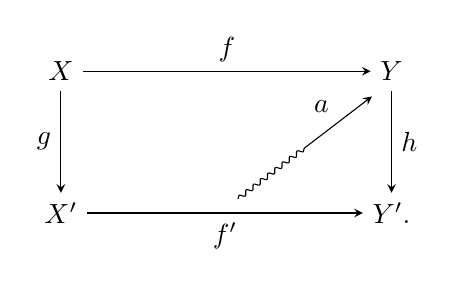
\begin{tikzpicture}[>=stealth,baseline=(current bounding box.center)]
    \node (X)  at (0,1.8) {$X$};
    \node (Y)  at (4.2,1.8) {$Y$};
    \node (Xp) at (0,0) {$X'$};
    \node (Yp) at (4.2,0) {$Y'\mathpunct{.}$};
    \draw[->] (X) -- node[above] {$f$} (Y);
    \draw[->] (X) -- node[left] {$g$} (Xp);
    \draw[->] (Y) -- node[right] {$h$} (Yp);
    \draw[->] (Xp) -- node[below] {$f'$} (Yp);
    \draw[decorate,decoration={snake,amplitude=0.8pt,segment length=3.3pt}]
      (2.25,0.18) -- (3.10,0.83);
    \draw[->] (3.10,0.83) -- node[above left] {$a$} (3.95,1.48);
  \end{tikzpicture}
  \tag{3.1.1.2}
\end{equation}

\VerdierSourcePageBlock{0083}%
\VerdierSemanticAnchor{ch1-3-1-1-additivity}
圏 $\operatorname{tr}_1(C)$ は加法圏である。$X\xrightarrow{f}Y$ と
$X'\xrightarrow{f'}Y'$ の直和は

\VerdierSemanticAnchor{ch1-3-1-1-direct-sum}
\begin{equation*}
  X\oplus X'
  \xrightarrow{\left(\begin{smallmatrix}f&0\\0&f'\end{smallmatrix}\right)}
  Y\oplus Y'
\end{equation*}
である。

\VerdierSemanticAnchor{ch1-3-1-2}
\noindent\textbf{3.1.2.}\quad
$X\xrightarrow{f}Y$ を $\operatorname{tr}_1(C)$ の対象とする。次のようにおく：

\VerdierSemanticAnchor{ch1-3-1-2-cone-object}
\begin{equation*}
  c(f)^i=Y^i\oplus X^{i+1},
\end{equation*}

\VerdierSemanticAnchor{ch1-3-1-2-eq1}
\begin{equation}
  d_{c(f)}^i=
  \begin{pmatrix}
    d_Y^i & f^{i+1}\\
    0 & -d_X^{i+1}
  \end{pmatrix}
  \colon Y^i\oplus X^{i+1}\longrightarrow Y^{i+1}\oplus X^{i+2}.
  \tag{3.1.2.1}
\end{equation}

\VerdierSemanticAnchor{ch1-3-1-2-cone-verification}
これにより $C$ の対象からなる複体が定義されたことが確かめられる。
\VerdierSemanticAnchor{ch1-3-1-2-cone-name}
この複体を $c(f)$ と書き、射 $f$ の\emph{写像錐}と呼ぶ。次に

\VerdierSemanticAnchor{ch1-3-1-2-morphism-setup}
\begin{equation*}
  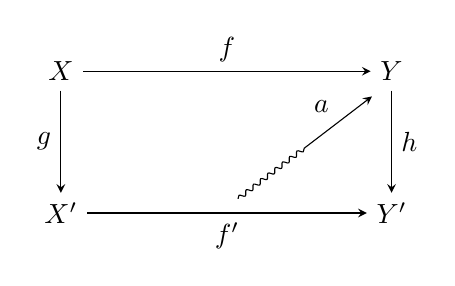
\begin{tikzpicture}[>=stealth,baseline=(current bounding box.center)]
    \node (X)  at (0,1.8) {$X$};
    \node (Y)  at (4.2,1.8) {$Y$};
    \node (Xp) at (0,0) {$X'$};
    \node (Yp) at (4.2,0) {$Y'$};
    \draw[->] (X) -- node[above] {$f$} (Y);
    \draw[->] (X) -- node[left] {$g$} (Xp);
    \draw[->] (Y) -- node[right] {$h$} (Yp);
    \draw[->] (Xp) -- node[below] {$f'$} (Yp);
    \draw[decorate,decoration={snake,amplitude=0.8pt,segment length=3.3pt}]
      (2.25,0.18) -- (3.10,0.83);
    \draw[->] (3.10,0.83) -- node[above left] {$a$} (3.95,1.48);
  \end{tikzpicture}
\end{equation*}
を $\operatorname{tr}_1(C)$ の射とする。次のようにおく：

\VerdierSemanticAnchor{ch1-3-1-2-eq2}
\begin{equation}
  c((g,h,a))^i=
  \begin{pmatrix}
    h^i & a^i\\
    0 & g^{i+1}
  \end{pmatrix}
  \colon Y^i\oplus X^{i+1}\longrightarrow Y'^i\oplus X'^{i+1}.
  \tag{3.1.2.2}
\end{equation}

\VerdierSemanticAnchor{ch1-3-1-2-complex-morphism}
これらの射は $c(f)$ と $c(f')$ の微分と可換であり、したがって複体の射

\VerdierSemanticAnchor{ch1-3-1-2-eq3}
\begin{equation}
  c((g,h,a))\colon c(f)\longrightarrow c(f')
  \tag{3.1.2.3}
\end{equation}
を定める。

\VerdierSemanticAnchor{ch1-3-1-2-cone-functor}
このようにして関手
$c\colon\operatorname{tr}_1(C)\longrightarrow\operatorname{comp}(C)$
が定義されたことが確かめられる。これを\emph{写像錐関手}と呼ぶ。

\VerdierSemanticAnchor{ch1-3-1-2-s-functor}
$s\colon\operatorname{comp}(C)\longrightarrow\operatorname{tr}_1(C)$ を
関手 $X\longmapsto(0\longrightarrow X)$ とする。
\VerdierSemanticAnchor{ch1-3-1-2-phi-setup}
$\operatorname{tr}_1(C)$ の各対象 $X\xrightarrow{f}Y$ に対し、
$\Phi(f)\colon(X\xrightarrow{f}Y)\longrightarrow s c(f)$ により%
\VerdierSourcePageContinue{0084}%
\VerdierSemanticAnchor{ch1-3-1-2-phi-definition-continuation}
$\operatorname{tr}_1(C)$ の次の射を表すものとする：

\VerdierSemanticAnchor{ch1-3-1-2-phi-diagram}
\begin{equation*}
  \Phi(f)=(0,p(f),a(f))
  \qquad
  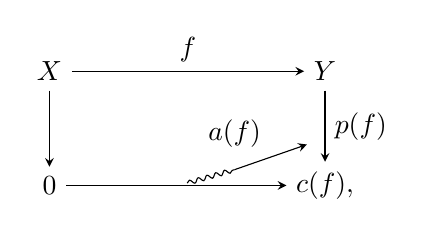
\begin{tikzpicture}[>=stealth,baseline=(current bounding box.center)]
    \node (X)  at (0,1.45) {$X$};
    \node (Y)  at (3.5,1.45) {$Y$};
    \node (Z)  at (0,0) {$0$};
    \node (Cf) at (3.5,0) {$c(f)\mathpunct{,}$};
    \draw[->] (X) -- node[above] {$f$} (Y);
    \draw[->] (X) -- (Z);
    \draw[->] (Y) -- node[right] {$p(f)$} (Cf);
    \draw[->] (Z) -- (Cf);
    \draw[decorate,decoration={snake,amplitude=0.8pt,segment length=3.3pt}]
      (1.75,0.03) -- (2.35,0.20);
    \draw[->] (2.35,0.20) -- node[above left] {$a(f)$} (3.27,0.52);
  \end{tikzpicture}
\end{equation*}

\VerdierSemanticAnchor{ch1-3-1-2-eq4}
\begin{equation}
  \begin{aligned}
    p(f)^i&=
      \begin{pmatrix}
        \operatorname{id}_{Y^i}\\[1mm]
        0
      \end{pmatrix}
      \colon Y^i\longrightarrow Y^i\oplus X^{i+1},\\[2mm]
    a(f)^i&=
      \begin{pmatrix}
        0\\[1mm]
        \operatorname{id}_{X^{i+1}}
      \end{pmatrix}
      \colon X^{i+1}\longrightarrow Y^i\oplus X^{i+1}.
  \end{aligned}
  \tag{3.1.2.4}
\end{equation}

\VerdierSemanticAnchor{ch1-3-1-2-phi-naturality}
直ちに計算すると、$\Phi$ は圏 $\operatorname{tr}_1(C)$ の恒等関手から
関手 $sc$ への関手の射であることがわかる。

\VerdierSemanticAnchor{ch1-3-1-3}
\noindent\textbf{命題 3.1.3.}\quad
\emph{射 $\Phi$ は写像錐関手を関手 $s$ の左随伴にする。すなわち、
$\operatorname{tr}_1(C)$ の各対象 $X\xrightarrow{f}Y$ と
$\operatorname{comp}(C)$ の各対象 $W$ に対し、射 $\Phi$ が定める標準写像}

\VerdierSemanticAnchor{ch1-3-1-3-hom-isomorphism}
\begin{equation*}
  \operatorname{Hom}_{\operatorname{comp}(C)}(c(f),W)
  \longrightarrow
  \operatorname{Hom}_{\operatorname{tr}_1(C)}
    \bigl((X\xrightarrow{f}Y),sW\bigr)
\end{equation*}
\emph{は同型である。}

\VerdierSemanticAnchor{ch1-3-1-3-verification}
検証は読者に委ねる。
\VerdierSemanticAnchor{ch1-3-1-3-s-fully-faithful}
関手 $s$ は充満忠実であり、したがって関手 $cs$ は恒等関手と標準的に同型である。
\VerdierSemanticAnchor{ch1-3-1-3-cs-identity}
実際、ここで選んだ関手 $c$ の構成では、関手 $cs$ は恒等関手に等しい。
\VerdierSemanticAnchor{ch1-3-1-3-adjunction-reformulation}
(3.1.3) の随伴性は次のようにも表せる。関手が定める写像

\VerdierSemanticAnchor{ch1-3-1-3-c-hom-isomorphism}
\begin{equation*}
  c\colon
  \operatorname{Hom}_{\operatorname{tr}_1(C)}
    \bigl((X\xrightarrow{f}Y),sW\bigr)
  \longrightarrow
  \operatorname{Hom}_{\operatorname{comp}(C)}(c(f),W)
\end{equation*}
は同型である。

\VerdierSemanticAnchor{ch1-3-1-4}
\noindent\textbf{3.1.4.}\quad
$\operatorname{tr}_1(C)$ にホモトピーの概念を定義する。次の二つの射を考える：

\VerdierSemanticAnchor{ch1-3-1-4-homotopy-setup}
\begin{equation*}
  (g,h,a),(g',h',a')\colon
  (X\xrightarrow{f}Y)
  \rightrightarrows
  (X'\xrightarrow{f'}Y')
\end{equation*}%
\VerdierSourcePageContinue{0085}%
\VerdierSemanticAnchor{ch1-3-1-4-homotopy-definition-continuation}
を $\operatorname{tr}_1(C)$ の二つの射とする。$(g,h,a)$ と
$(g',h',a')$ を結ぶ\emph{ホモトピー}とは三つ組 $(b,b',\alpha)$ であり、
$b\colon g\rightsquigarrow g'$ と $b'\colon h\rightsquigarrow h'$ は
ホモトピーで、

\VerdierSemanticAnchor{ch1-3-1-4-second-order-condition}
\begin{equation*}
  \alpha\colon f'\star b+a'\rightsquigarrow b'\star f+a
\end{equation*}
は二階ホモトピー (2.5.12) である。

\VerdierSemanticAnchor{ch1-3-1-4-homotopic-morphisms}
$\operatorname{tr}_1(C)$ の二つの射は、それらを結ぶホモトピーが存在するとき、
\emph{ホモトピック}であるという。
\VerdierSemanticAnchor{ch1-3-1-4-equivalence-relation}
「$(g,h,a)$ と $(g',h',a')$ はホモトピックである」という関係は、射の直和と
合成に両立する同値関係である。
\VerdierSemanticAnchor{ch1-3-1-4-tr1-homotopy-category}
したがって、対象を $\operatorname{tr}_1(C)$ の対象、射を
$\operatorname{tr}_1(C)$ の射のホモトピー類とする圏
$\operatorname{Tr}_1(C)$ を導入できる。

\VerdierSemanticAnchor{ch1-3-1-5}
\noindent\textbf{命題 3.1.5.}\quad
\emph{
$D,D'\colon (X\xrightarrow{f}Y)\rightrightarrows
(X'\xrightarrow{f'}Y')$ を $\operatorname{tr}_1(C)$ の二つの射とする。
$D$ と $D'$ が $\operatorname{tr}_1(C)$ でホモトピックならば、$c(D)$ と
$c(D')$ は $\operatorname{comp}(C)$ でホモトピックである。}

\VerdierSemanticAnchor{ch1-3-1-5-proof-setup}
$D=(g,h,a)$、$D'=(g',h',a')$ とする。$D$ と $D'$ が
$\operatorname{tr}_1(C)$ でホモトピックであると仮定する。このとき、次を満たす
ホモトピー $b,b'$ が存在する：

\VerdierSemanticAnchor{ch1-3-1-5-eq1}
\begin{equation}
  \begin{aligned}
    g'-g&=bd+db,\\
    h'-h&=b'd+db'.
  \end{aligned}
  \tag{3.1.5.1}
\end{equation}

（記号を軽くするため、この計算では各成分の次数を表す上付き添字を省いた。）
\VerdierSemanticAnchor{ch1-3-1-5-second-order-homotopy}
さらに、次を満たす二階ホモトピー $\alpha$ が存在する：
\begin{equation*}
  \alpha d-d\alpha=b'f+a-(f'b+a').
\end{equation*}

\VerdierSemanticAnchor{ch1-3-1-5-cone-homotopy}
直ちに計算すると
\begin{equation*}
  \begin{pmatrix}
    b' & \alpha\\
    0  & -b
  \end{pmatrix}
\end{equation*}
が $c(D)$ と $c(D')$ を結ぶホモトピーであることがわかる。

\VerdierSemanticAnchor{ch1-3-1-6}
\noindent\textbf{系 3.1.6.}\quad
\emph{関手}
\begin{equation*}
  c\colon\operatorname{tr}_1(C)\longrightarrow\operatorname{comp}(C)
  \qquad\text{および}\qquad
  s\colon\operatorname{comp}(C)\longrightarrow\operatorname{tr}_1(C)
\end{equation*}
\emph{は $\operatorname{tr}_1(C)$ と $\operatorname{comp}(C)$ のホモトピーに
両立し、商をとることにより、やはり}

\VerdierSemanticAnchor{ch1-3-1-6-descended-functors}
\begin{equation*}
  c\colon\operatorname{Tr}_1(C)\longrightarrow K(C)
  \qquad\text{および}\qquad
  s\colon K(C)\longrightarrow\operatorname{Tr}_1(C)
\end{equation*}
\emph{と書かれる関手を定める。}
\VerdierSemanticAnchor{ch1-3-1-6-adjunction}
\emph{関手 $c\colon\operatorname{Tr}_1(C)\longrightarrow K(C)$ は関手
$s\colon K(C)\longrightarrow\operatorname{Tr}_1(C)$ の左随伴である。}

\VerdierSemanticAnchor{ch1-3-1-6-proof}
これは (3.1.5) と (3.1.3) から形式的に従う。

\VerdierSemanticAnchor{ch1-3-1-7}
\noindent\textbf{3.1.7.}\quad
\VerdierSemanticAnchor{ch1-3-1-7-s-prime}
$s'\colon\operatorname{comp}(C)\longrightarrow\operatorname{tr}_1(C)$ を
関手 $X\longmapsto(X\longrightarrow 0)$ とする。
\VerdierSemanticAnchor{ch1-3-1-7-comp-translation}
関手 $cs'\colon\operatorname{comp}(C)\longrightarrow\operatorname{comp}(C)$
は $\operatorname{comp}(C)$ のシフト関手に等しい。
\VerdierSemanticAnchor{ch1-3-1-7-descended-s-prime}
関手 $s'$ は $\operatorname{comp}(C)$ のホモトピックな二つの射を
$\operatorname{tr}_1(C)$ のホモトピックな射に送り、したがって、やはり $s'$ と
書かれる関手 $s'\colon K(C)\longrightarrow\operatorname{Tr}_1(C)$ を定める。
\VerdierSemanticAnchor{ch1-3-1-7-k-translation}
関手 $cs'\colon K(C)\longrightarrow K(C)$ は $K(C)$ のシフト関手に等しい。

\VerdierSourcePageBlock{0086}%
\VerdierSemanticAnchor{ch1-3-2}
\subsection{写像錐関手の性質}

\VerdierSemanticAnchor{ch1-3-2-1}
\noindent\textbf{3.2.1.}\quad
\VerdierSemanticAnchor{ch1-3-2-1-triangle-definition}
$\mathbb Z$-圏において、次の形の任意の図式を\emph{三角}と呼ぶ：

\VerdierSemanticAnchor{ch1-3-2-1-eq1}
\begin{equation}
  X\xrightarrow{u}Y\xrightarrow{v}Z\xrightarrow{w}X[1].
  \tag{3.2.1.1}
\end{equation}

\VerdierSemanticAnchor{ch1-3-2-1-notation}
三角 (3.2.1.1) を表すには、記号 $(X,Y,Z,u,v,w)$ または次の図式を用いる：

\VerdierSemanticAnchor{ch1-3-2-1-eq2}
\begin{equation}
  \begin{tikzpicture}[>=stealth,baseline=(current bounding box.center)]
    \node (X) at (0,0) {$X$};
    \node (Y) at (4.2,0) {$Y\mathpunct{,}$};
    \node (Z) at (2.1,1.65) {$Z$};
    \draw[->] (X) -- node[above] {$u$} (Y);
    \draw[->] (Y) -- node[right] {$v$} (Z);
    \draw[->] (Z) -- node[left] {$w$} (X);
    \draw[line width=0.45pt] (1.91,1.50) -- (1.91,1.67);
  \end{tikzpicture}
  \tag{3.2.1.2}
\end{equation}

\VerdierSemanticAnchor{ch1-3-2-1-pusher-mark}
ここで短い線の印を付した矢印は、三角の次数 $1$ の射を表す。
\VerdierSemanticAnchor{ch1-3-2-1-triangle-morphism}
$(X,Y,Z,u,v,w)$ と $(X',Y',Z',u',v',w')$ を二つの三角とする。
\emph{三角の射}とは、次の可換図式をいう：

\VerdierSemanticAnchor{ch1-3-2-1-eq3}
\begin{equation}
  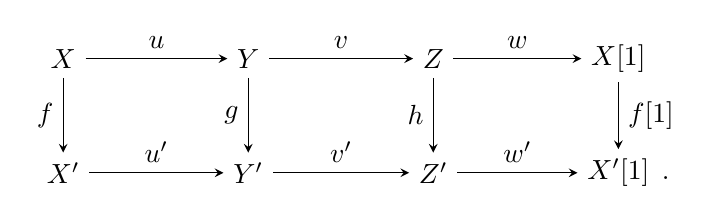
\begin{tikzpicture}[>=stealth,baseline=(current bounding box.center)]
    \node (X)  at (0,1.45) {$X$};
    \node (Y)  at (2.35,1.45) {$Y$};
    \node (Z)  at (4.70,1.45) {$Z$};
    \node (Xs) at (7.05,1.45) {$X[1]$};
    \node (Xp) at (0,0) {$X'$};
    \node (Yp) at (2.35,0) {$Y'$};
    \node (Zp) at (4.70,0) {$Z'$};
    \node (Xps) at (7.05,0) {$X'[1]$};
    \node[anchor=base west,inner sep=0pt,xshift=.08em] at (Xps.base east) {$.$};
    \draw[->] (X) -- node[above] {$u$} (Y);
    \draw[->] (Y) -- node[above] {$v$} (Z);
    \draw[->] (Z) -- node[above] {$w$} (Xs);
    \draw[->] (Xp) -- node[above] {$u'$} (Yp);
    \draw[->] (Yp) -- node[above] {$v'$} (Zp);
    \draw[->] (Zp) -- node[above] {$w'$} (Xps);
    \draw[->] (X) -- node[left] {$f$} (Xp);
    \draw[->] (Y) -- node[left] {$g$} (Yp);
    \draw[->] (Z) -- node[left] {$h$} (Zp);
    \draw[->] (Xs) -- node[right] {$f[1]$} (Xps);
  \end{tikzpicture}
  \tag{3.2.1.3}
\end{equation}

\VerdierSemanticAnchor{ch1-3-2-1-morphism-composition}
三角の射は明らかな仕方で合成される。
\VerdierSemanticAnchor{ch1-3-2-1-triangle-category}
三角は一つの圏をなす。

\VerdierSemanticAnchor{ch1-3-2-2}
\noindent\textbf{3.2.2.}\quad
\VerdierSemanticAnchor{ch1-3-2-2-source-morphism}
$X\xrightarrow{f}Y$ を $\operatorname{tr}_1(C)$ の対象とする。次の
$\operatorname{tr}_1(C)$ の射（$f$ に関して関手的な射）を考える：

\VerdierSemanticAnchor{ch1-3-2-2-eq1}
\begin{equation}
  \begin{tikzpicture}[>=stealth,baseline=(current bounding box.center)]
    \node (X)  at (0,1.35) {$X$};
    \node (Y)  at (3.6,1.35) {$Y$};
    \node (Xp) at (0,0) {$X$};
    \node (Z)  at (3.6,0) {$0$};
    \node[anchor=base west,inner sep=0pt,xshift=.08em] at (Z.base east) {$,$};
    \draw[->] (X) -- node[above] {$f$} (Y);
    \draw[->] (X) -- node[left] {$\operatorname{id}_X$} (Xp);
    \draw[->] (Y) -- (Z);
    \draw[->] (Xp) -- (Z);
  \end{tikzpicture}
  \tag{3.2.2.1}
\end{equation}

\VerdierSemanticAnchor{ch1-3-2-2-cone-application}
これに写像錐関手を適用すると、$X\xrightarrow{f}Y$ に関して関手的な
$\operatorname{comp}(C)$ の射 (3.1.7)

\VerdierSemanticAnchor{ch1-3-2-2-eq2}
\begin{equation}
  q(f)\colon c(f)\longrightarrow X[1]
  \tag{3.2.2.2}
\end{equation}
が得られる。

\VerdierSourcePageBlock{0087}%
\VerdierSemanticAnchor{ch1-3-2-2-dual-morphism}
同様に、$\operatorname{tr}_1(C)$ の射

\VerdierSemanticAnchor{ch1-3-2-2-eq3}
\begin{equation}
  \begin{tikzpicture}[>=stealth,baseline=(current bounding box.center)]
    \node (Z)  at (0,1.35) {$0$};
    \node (Y)  at (3.6,1.35) {$Y$};
    \node (X)  at (0,0) {$X$};
    \node (Yp) at (3.6,0) {$Y$};
    \draw[->] (Z) -- (Y);
    \draw[->] (Z) -- (X);
    \draw[->] (Y) -- node[right] {$\operatorname{id}_Y$} (Yp);
    \draw[->] (X) -- node[above] {$f$} (Yp);
  \end{tikzpicture}
  \tag{3.2.2.3}
\end{equation}

\VerdierSemanticAnchor{ch1-3-2-2-cone-entry-p}
に写像錐関手を適用すると、$X\xrightarrow{f}Y$ に関して関手的な
$\operatorname{comp}(C)$ の射 (3.1.2.4)

\VerdierSemanticAnchor{ch1-3-2-2-eq4}
\begin{equation}
  p(f)\colon Y\longrightarrow c(f)
  \tag{3.2.2.4}
\end{equation}
が得られる。

\VerdierSemanticAnchor{ch1-3-2-2-comp-triangle}
したがって、$\operatorname{tr}_1(C)$ の各対象 $X\xrightarrow{f}Y$ に
$\operatorname{comp}(C)$ の三角

\VerdierSemanticAnchor{ch1-3-2-2-eq5}
\begin{equation}
  X\xrightarrow{f}Y\xrightarrow{p(f)}c(f)\xrightarrow{q(f)}X[1]
  \tag{3.2.2.5}
\end{equation}
を対応させることができる。

\VerdierSemanticAnchor{ch1-3-2-2-nonfunctoriality}
この三角は、$\operatorname{tr}_1(C)$ の対象 $X\xrightarrow{f}Y$ に
関手的には依存しないことに注意する。
\VerdierSemanticAnchor{ch1-3-2-2-morphism-d-setup}
実際、
$D=(g,h,a)\colon(X\xrightarrow{f}Y)\longrightarrow
(X'\xrightarrow{f'}Y')$
を $\operatorname{tr}_1(C)$ の射とする。このとき次の図式を得る：

\VerdierSemanticAnchor{ch1-3-2-2-eq6}
\begin{equation}
  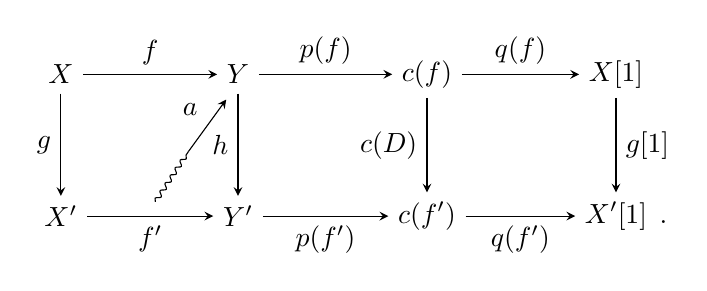
\begin{tikzpicture}[>=stealth,baseline=(current bounding box.center)]
    \node (X)   at (0,1.8) {$X$};
    \node (Y)   at (2.25,1.8) {$Y$};
    \node (C)   at (4.65,1.8) {$c(f)$};
    \node (Xs)  at (7.05,1.8) {$X[1]$};
    \node (Xp)  at (0,0) {$X'$};
    \node (Yp)  at (2.25,0) {$Y'$};
    \node (Cp)  at (4.65,0) {$c(f')$};
    \node (Xps) at (7.05,0) {$X'[1]$};
    \node[anchor=base west,inner sep=0pt,xshift=.08em] at (Xps.base east) {$.$};
    \draw[->] (X) -- node[above] {$f$} (Y);
    \draw[->] (Y) -- node[above] {$p(f)$} (C);
    \draw[->] (C) -- node[above] {$q(f)$} (Xs);
    \draw[->] (Xp) -- node[below] {$f'$} (Yp);
    \draw[->] (Yp) -- node[below] {$p(f')$} (Cp);
    \draw[->] (Cp) -- node[below] {$q(f')$} (Xps);
    \draw[->] (X) -- node[left] {$g$} (Xp);
    \draw[->] (Y) -- node[left] {$h$} (Yp);
    \draw[->] (C) -- node[left] {$c(D)$} (Cp);
    \draw[->] (Xs) -- node[right] {$g[1]$} (Xps);
    \draw[decorate,decoration={snake,amplitude=0.8pt,segment length=3.3pt}]
      (1.20,0.18) -- (1.62,0.82);
    \draw[->] (1.62,0.82) -- node[above left] {$a$} (2.10,1.48);
  \end{tikzpicture}
  \tag{3.2.2.6}
\end{equation}

\VerdierSemanticAnchor{ch1-3-2-2-square-commutativity}
射 $p(f)$ と $q(f)$ は $f$ に関して関手的であるから、この図式の後ろ二つの
正方形は可換であるが、最初の正方形はホモトピーを除いてのみ可換である。
\VerdierSemanticAnchor{ch1-3-2-2-quotient-triangle}
ホモトピーで商をとると、$\operatorname{Tr}_1(C)$ の各対象
$X\xrightarrow{f}Y$ に $K(C)$ の三角

\VerdierSemanticAnchor{ch1-3-2-2-eq7}
\begin{equation}
  X\xrightarrow{\dot f}Y\xrightarrow{\dot p(f)}c(f)
  \xrightarrow{\dot q(f)}X[1]
  \tag{3.2.2.7}
\end{equation}
\VerdierSemanticAnchor{ch1-3-2-2-homotopy-class-notation}
を関手的に対応させることができる。（$\dot f$、$\dot p(f)$、
$\dot q(f)$ は、それぞれ射 $f$、$p(f)$、$q(f)$ のホモトピー類を表す。）
\VerdierSemanticAnchor{ch1-3-2-2-triangle-functor}
こうして、圏 $\operatorname{Tr}_1(C)$ から $K(C)$ における三角の圏への
関手を得る。

\VerdierSourcePageBlock{0088}%
\VerdierSemanticAnchor{ch1-3-2-3}
\noindent\textbf{3.2.3.}\quad
\VerdierSemanticAnchor{ch1-3-2-3-translation-automorphism}
$\operatorname{comp}(C)$ のシフト自己同型は、自然に自己同型
$T\colon\operatorname{tr}_1(C)\longrightarrow\operatorname{tr}_1(C)$ に延長される：

\VerdierSemanticAnchor{ch1-3-2-3-eq1}
\begin{equation}
  \begin{aligned}
    T\bigl(X\xrightarrow{f}Y\bigr)
      &=X[1]\xrightarrow{f[1]}Y[1],\\
    T((g,h,a))&=(g[1],h[1],-a[1]).
  \end{aligned}
  \tag{3.2.3.1}
\end{equation}

\VerdierSemanticAnchor{ch1-3-2-3-cone-z-functor}
次に、同型
\VerdierSemanticAnchor{ch1-3-2-3-psi-isomorphism}
$\Psi(f)\colon c(f[1])\xrightarrow{\sim}c(f)[1]$ を定めることにより、
写像錐関手を $\mathbb Z$-関手 (1.5.2) にする：

\VerdierSemanticAnchor{ch1-3-2-3-eq2}
\begin{equation}
  \Psi(f)^i=
  \begin{pmatrix}
    \operatorname{id}_{Y^{i+1}} & 0\\
    0 & -\operatorname{id}_{X^{i+2}}
  \end{pmatrix}
  \colon Y^{i+1}\oplus X^{i+2}
  \longrightarrow Y^{i+1}\oplus X^{i+2}.
  \tag{3.2.3.2}
\end{equation}

\VerdierSemanticAnchor{ch1-3-2-3-reader-verification}
(3.2.3.2) が実際に複体の同型を定めることを読者は確かめ、次の命題を証明されたい：

\VerdierSemanticAnchor{ch1-3-2-4}
\noindent\textbf{命題 3.2.4.}\quad
\VerdierSemanticAnchor{ch1-3-2-4-zero-source}
\emph{$f=0\longrightarrow Y$ のとき、標準同型}
\begin{equation*}
  c(f[n])\xrightarrow{\sim}c(f)[n]
\end{equation*}
\emph{は $Y[n]$ の恒等写像にほかならない。$f=X\longrightarrow0$ のとき、
標準同型}
\VerdierSemanticAnchor{ch1-3-2-4-zero-target}
\begin{equation*}
  c(f[n])\xrightarrow{\sim}c(f)[n]
\end{equation*}
\emph{は同型}
\begin{equation*}
  X[n+1]\xrightarrow{(-1)^n\operatorname{id}_{X[n+1]}}X[n+1]
\end{equation*}
\emph{にほかならない。}

\VerdierSemanticAnchor{ch1-3-2-5}
\noindent\textbf{3.2.5.}\quad
$X\xrightarrow{f}Y$ を $\operatorname{tr}_1(C)$ の対象とする。これに
$\operatorname{comp}(C)$ の三角

\VerdierSemanticAnchor{ch1-3-2-5-triangle}
\VerdierSemanticAnchor{ch1-3-2-5-eq1}
\begin{equation}
  Y\xrightarrow{p(f)}c(f)\xrightarrow{q(f)}X[1]
  \xrightarrow{f[1]}Y[1]
  \tag{3.2.5.1}
\end{equation}
を対応させることができる。

\VerdierSemanticAnchor{ch1-3-2-5-composite}
射 $q(f)p(f)\colon Y\longrightarrow X[1]$ は、次の射の写像錐関手による像である：

\VerdierSemanticAnchor{ch1-3-2-5-cone-morphism-diagram}
\begin{equation*}
  \begin{tikzpicture}[>=stealth,baseline=(current bounding box.center)]
    \node (Z1) at (0,1.45) {$0$};
    \node (Y)  at (3.5,1.45) {$Y$};
    \node (X)  at (0,0) {$X$};
    \node (Z2) at (3.5,0) {$0$};
    \node[anchor=base west,inner sep=0pt,xshift=.08em] at (Z2.base east) {$.$};
    \draw[->] (Z1) -- (Y);
    \draw[->] (Z1) -- (X);
    \draw[->] (Y) -- (Z2);
    \draw[->] (X) -- (Z2);
  \end{tikzpicture}
\end{equation*}%
\VerdierSourcePageContinue{0089}%
\VerdierSemanticAnchor{ch1-3-2-5-composite-zero-conclusion}
したがってこれは零である。よって、写像錐関手の随伴性 (3.1.3) により、
一意な射

\VerdierSemanticAnchor{ch1-3-2-5-eq2}
\begin{equation}
  J\colon c(p(f))\longrightarrow X[1]
  \tag{3.2.5.2}
\end{equation}

\noindent が存在し、次の図式が可換となる：

\VerdierSemanticAnchor{ch1-3-2-5-eq3}
\VerdierSemanticAnchor{ch1-3-2-5-j-comparison-diagram}
\begin{equation}
  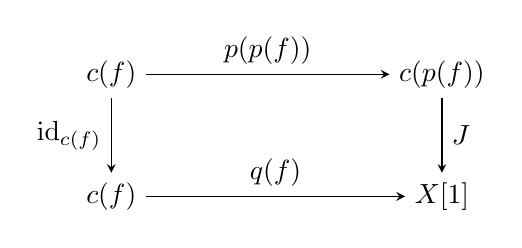
\begin{tikzpicture}[>=stealth,baseline=(current bounding box.center)]
    \node (Cf1) at (0,1.55) {$c(f)$};
    \node (Cpf) at (4.2,1.55) {$c(p(f))$};
    \node (Cf2) at (0,0) {$c(f)$};
    \node (Xs)  at (4.2,0) {$X[1]$};
    \draw[->] (Cf1) -- node[above] {$p(p(f))$} (Cpf);
    \draw[->] (Cf1) -- node[left] {$\operatorname{id}_{c(f)}$} (Cf2);
    \draw[->] (Cpf) -- node[right] {$J$} (Xs);
    \draw[->] (Cf2) -- node[above] {$q(f)$} (Xs);
  \end{tikzpicture}
  \tag{3.2.5.3}
\end{equation}

\noindent さらに $Ja(p(f))=0$ (3.1.2.4) である。

\VerdierSemanticAnchor{ch1-3-2-6}
\noindent\textbf{命題 3.2.6.}\quad
\VerdierSemanticAnchor{ch1-3-2-6-a}
\emph{a) 射 $J$ はホモトピー同値、すなわちホモトピーを除いて同型である。}

\VerdierSemanticAnchor{ch1-3-2-6-b}
\emph{b) 次の図式}

\VerdierSemanticAnchor{ch1-3-2-6-eq1}
\begin{equation}
  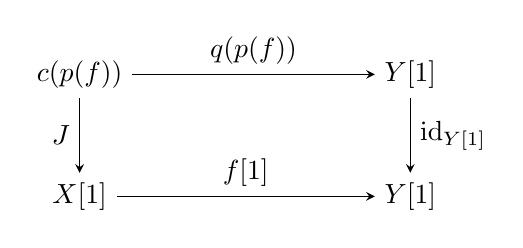
\begin{tikzpicture}[>=stealth,baseline=(current bounding box.center)]
    \node (Cpf) at (0,1.55) {$c(p(f))$};
    \node (Ys1) at (4.2,1.55) {$Y[1]$};
    \node (Xs)  at (0,0) {$X[1]$};
    \node (Ys2) at (4.2,0) {$Y[1]$};
    \draw[->] (Cpf) -- node[above] {$q(p(f))$} (Ys1);
    \draw[->] (Cpf) -- node[left] {$J$} (Xs);
    \draw[->] (Ys1) -- node[right] {$\operatorname{id}_{Y[1]}$} (Ys2);
    \draw[->] (Xs) -- node[above] {$f[1]$} (Ys2);
  \end{tikzpicture}
  \tag{3.2.6.1}
\end{equation}

\noindent\emph{はホモトピーを除いて反可換である。}

\VerdierSemanticAnchor{ch1-3-2-7}
\noindent\textbf{3.2.7. 証明。}\quad
\VerdierSemanticAnchor{ch1-3-2-7-h-construction}
まず射 $H\colon X[1]\longrightarrow c(p(f))$ を構成する。
\VerdierSemanticAnchor{ch1-3-2-7-representing-functors}
そのためには、この二つの対象が表現する二つの関手の間の射を構成すればよい。
$W$ を $\operatorname{comp}(C)$ の対象とする。
\VerdierSemanticAnchor{ch1-3-2-7-pair}
写像錐関手の随伴性 (3.1.3) を考慮すれば、$c(p(f))$ から $W$ への射とは、
$u\colon c(f)\longrightarrow W$ が複体の射で、
$a\colon0\rightsquigarrow up(f)$ がホモトピーであるような組 $(u,a)$ に
ほかならない。
\VerdierSemanticAnchor{ch1-3-2-7-triple}
再び (3.1.3) を用いると、$c(p(f))$ から $W$ への射は三つ組
\begin{equation*}
  \bigl(m\colon Y\longrightarrow W,\quad
  a\colon0\rightsquigarrow m,\quad
  b\colon0\rightsquigarrow mf\bigr)
\end{equation*}
であることがわかる。この三つ組に次の図式を対応させる：

\VerdierSemanticAnchor{ch1-3-2-7-eq1}
\begin{equation}
  \begin{gathered}
    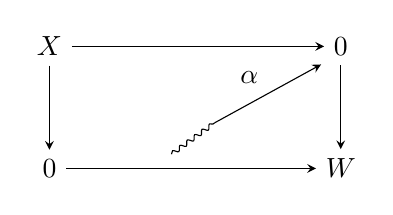
\begin{tikzpicture}[>=stealth,baseline=(current bounding box.center)]
      \node (X)  at (0,1.55) {$X$};
      \node (Z1) at (3.7,1.55) {$0$};
      \node (Z2) at (0,0) {$0$};
      \node (W)  at (3.7,0) {$W$};
      \draw[->] (X) -- (Z1);
      \draw[->] (X) -- (Z2);
      \draw[->] (Z1) -- (W);
      \draw[->] (Z2) -- (W);
      \draw[decorate,decoration={snake,amplitude=0.8pt,segment length=3.3pt}]
        (1.55,0.18) -- (2.10,0.58);
      \draw[->] (2.10,0.58) -- node[above left] {$\alpha$} (3.45,1.32);
    \end{tikzpicture}
    \qquad \alpha=b-a\star f ,
  \end{gathered}
  \tag{3.2.7.1}
\end{equation}%
\VerdierSourcePageContinue{0090}%
\VerdierSemanticAnchor{ch1-3-2-7-representing-functor-continuation}
すなわち、(3.1.3) と (3.1.7) により $X[1]$ から $W$ への射を対応させる。
こうして $W$ に関して関手的に、$c(p(f))$ から $W$ への各射に $X[1]$ から
$W$ への射を対応させたので、射
\VerdierSemanticAnchor{ch1-3-2-7-h-defined}
$H\colon X[1]\longrightarrow c(p(f))$ が定まった。

命題 (3.2.6) の a) を証明するには、次を示せば十分である：

\VerdierSemanticAnchor{ch1-3-2-7-eq2}
\begin{equation}
  \textit{射 }JH\colon X[1]\longrightarrow X[1]
  \textit{ は恒等射である。}
  \tag{3.2.7.2}
\end{equation}

\VerdierSemanticAnchor{ch1-3-2-7-eq3}
\begin{equation}
  \textit{射 }HJ\colon c(p(f))\longrightarrow c(p(f))
  \textit{ は恒等射とホモトピックである。}
  \tag{3.2.7.3}
\end{equation}

命題 (3.2.6) の b) を証明するには、さらに次を示せば十分である：

\VerdierSemanticAnchor{ch1-3-2-7-eq4}
\begin{equation}
  \begin{gathered}
    \textit{次の図式：}\\[0.35em]
    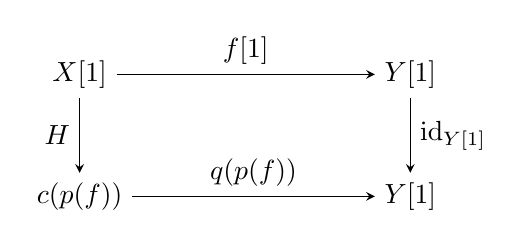
\begin{tikzpicture}[>=stealth,baseline=(current bounding box.center)]
      \node (Xs)  at (0,1.55) {$X[1]$};
      \node (Ys1) at (4.2,1.55) {$Y[1]$};
      \node (Cpf) at (0,0) {$c(p(f))$};
      \node (Ys2) at (4.2,0) {$Y[1]$};
      \draw[->] (Xs) -- node[above] {$f[1]$} (Ys1);
      \draw[->] (Xs) -- node[left] {$H$} (Cpf);
      \draw[->] (Ys1) -- node[right] {$\operatorname{id}_{Y[1]}$} (Ys2);
      \draw[->] (Cpf) -- node[above] {$q(p(f))$} (Ys2);
    \end{tikzpicture}\\[-0.15em]
    \textit{は反可換である。}
  \end{gathered}
  \tag{3.2.7.4}
\end{equation}

\VerdierSemanticAnchor{ch1-3-2-8}
\noindent\textbf{3.2.8. 主張 (3.2.7.2) の証明。}\quad
\VerdierSemanticAnchor{ch1-3-2-8-jh-identity-proof}
射 $JH\colon X[1]\longrightarrow X[1]$ が恒等射であることを示そう。
そのためには、射 $JH$ が $X[1]$ によって表現される関手の恒等自己準同型を
誘導することを確かめれば十分である。
\VerdierSemanticAnchor{ch1-3-2-8-represented-hom-functor}
(3.1.3) と (3.1.7) により、関手
\begin{equation*}
  W\longmapsto
  \operatorname{Hom}_{\operatorname{comp}(C)}(X[1],W)
\end{equation*}
は次の関手にほかならない：

\VerdierSemanticAnchor{ch1-3-2-8-eq1}
\begin{equation}
  W\longmapsto
  \left\{\,
  \vcenter{\hbox{%
    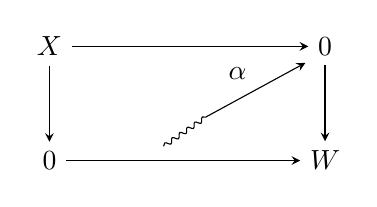
\begin{tikzpicture}[>=stealth,baseline=(current bounding box.center)]
      \node (X)  at (0,1.45) {$X$};
      \node (Z1) at (3.5,1.45) {$0$};
      \node (Z2) at (0,0) {$0$};
      \node (W)  at (3.5,0) {$W$};
      \draw[->] (X) -- (Z1);
      \draw[->] (X) -- (Z2);
      \draw[->] (Z1) -- (W);
      \draw[->] (Z2) -- (W);
      \draw[decorate,decoration={snake,amplitude=0.8pt,segment length=3.3pt}]
        (1.45,0.18) -- (2.00,0.56);
      \draw[->] (2.00,0.56) -- node[above left] {$\alpha$} (3.25,1.24);
    \end{tikzpicture}%
  }}\,\right\}.
  \tag{3.2.8.1}
\end{equation}

\VerdierSemanticAnchor{ch1-3-2-8-cpf-represented-functor}
一方、(3.2.7) により、$\operatorname{comp}(C)$ の対象 $c(p(f))$ は関手

\VerdierSemanticAnchor{ch1-3-2-8-eq2}
\begin{equation}
  W\longmapsto
  \left\{\,
  \bigl(m\colon Y\longrightarrow W,\quad
  a\colon0\rightsquigarrow m,\quad
  b\colon0\rightsquigarrow mf\bigr)
  \,\right\}
  \tag{3.2.8.2}
\end{equation}
を表現する。%
\VerdierSourcePageContinue{0091}%
\VerdierSemanticAnchor{ch1-3-2-8-j-induced-functorial-map}
射 $J\colon c(p(f))\longrightarrow X[1]$ は、直ちに確かめられるように、
次の関手の射に対応する：

\VerdierSemanticAnchor{ch1-3-2-8-eq3}
\begin{equation}
  \begin{gathered}
    D=
    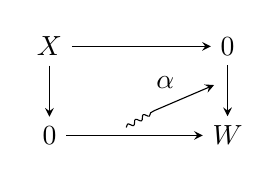
\begin{tikzpicture}[>=stealth,baseline=(current bounding box.center),
      scale=0.78,every node/.style={}]
      \node (X)  at (0,1.45) {$X$};
      \node (Z1) at (2.9,1.45) {$0$};
      \node (Z2) at (0,0) {$0$};
      \node (W)  at (2.9,0) {$W$};
      \draw[->] (X) -- (Z1);
      \draw[->] (X) -- (Z2);
      \draw[->] (Z1) -- (W);
      \draw[->] (Z2) -- (W);
      \draw[decorate,decoration={snake,amplitude=0.8pt,segment length=3.3pt}]
        (1.25,0.13) -- (1.70,0.40);
      \draw[->] (1.70,0.40) -- node[above left] {$\alpha$} (2.68,0.82);
    \end{tikzpicture}
    \quad\longmapsto\quad
    JD=\bigl(0\colon Y\longrightarrow W,\;
      0\colon0\rightsquigarrow0,\;
      \alpha\colon0\rightsquigarrow0\bigr).
  \end{gathered}
  \tag{3.2.8.3}
\end{equation}

\VerdierSemanticAnchor{ch1-3-2-8-h-induced-functorial-map}
射 $H\colon X[1]\longrightarrow c(p(f))$ は、定義 (3.2.7) により
次の関手の射に対応する：

\VerdierSemanticAnchor{ch1-3-2-8-eq4}
\begin{equation}
  \begin{aligned}
    t={}&\bigl(m\colon Y\longrightarrow W,\;
      a\colon0\rightsquigarrow m,\;
      b\colon0\rightsquigarrow mf\bigr)\\[-0.2em]
    &\longmapsto\quad Ht=
    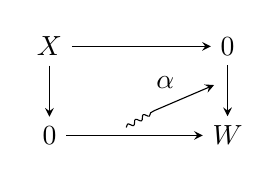
\begin{tikzpicture}[>=stealth,baseline=(current bounding box.center),
      scale=0.78,every node/.style={}]
      \node (X)  at (0,1.45) {$X$};
      \node (Z1) at (2.9,1.45) {$0$};
      \node (Z2) at (0,0) {$0$};
      \node (W)  at (2.9,0) {$W$};
      \draw[->] (X) -- (Z1);
      \draw[->] (X) -- (Z2);
      \draw[->] (Z1) -- (W);
      \draw[->] (Z2) -- (W);
      \draw[decorate,decoration={snake,amplitude=0.8pt,segment length=3.3pt}]
        (1.25,0.13) -- (1.70,0.40);
      \draw[->] (1.70,0.40) -- node[above left] {$\alpha$} (2.68,0.82);
    \end{tikzpicture}
    ,\qquad \alpha=b-a\star f.
  \end{aligned}
  \tag{3.2.8.4}
\end{equation}

\VerdierSemanticAnchor{ch1-3-2-8-composite-identity}
この二つの関手の射の合成は実際に恒等であり、これにより主張
(3.2.7.2) が証明される。

\VerdierSemanticAnchor{ch1-3-2-9}
\noindent\textbf{3.2.9. 主張 (3.2.7.3) の証明。}\quad
\VerdierSemanticAnchor{ch1-3-2-9-hj-functorial-map}
(3.2.8) により、射
$HJ\colon c(p(f))\longrightarrow c(p(f))$ は次の関手の射に対応する：

\VerdierSemanticAnchor{ch1-3-2-9-eq1}
\begin{equation}
  \begin{aligned}
    t={}&\bigl(m\colon Y\longrightarrow W,\;
      a\colon0\rightsquigarrow m,\;
      b\colon0\rightsquigarrow mf\bigr)
      \longmapsto HJt\\
    ={}&\bigl(0\colon Y\longrightarrow W,\;
      0\colon0\rightsquigarrow0,\;
      b-a\star f\colon0\rightsquigarrow0\bigr)
  \end{aligned}
  \tag{3.2.9.1}
\end{equation}
したがって：

\VerdierSemanticAnchor{ch1-3-2-9-eq2}
\begin{equation}
  t-HJt=\bigl(m\colon Y\longrightarrow W,\;
    a\colon0\rightsquigarrow m,\;
    a\star f\colon0\rightsquigarrow mf\bigr).
  \tag{3.2.9.2}
\end{equation}

\VerdierSemanticAnchor{ch1-3-2-9-null-homotopy-reduction}
主張 (3.2.7.3) を証明するには、
$\bigl(m\colon Y\longrightarrow W,\;a\colon0\rightsquigarrow m,\;
a\star f\colon0\rightsquigarrow mf\bigr)$ の形の任意の三つ組が、
$c(p(f))$ から $W$ への零にホモトピックな射に対応することを示せばよい。
(3.1.3) を用いると、このような三つ組は射

\VerdierSemanticAnchor{ch1-3-2-9-eq3}
\begin{equation}
  v\colon c(f)\longrightarrow W,
  \qquad
  v=\bigl(m\colon Y\longrightarrow W,\;
    a\star f\colon0\rightsquigarrow mf\bigr)
  \tag{3.2.9.3}
\end{equation}
とホモトピー

\VerdierSemanticAnchor{ch1-3-2-9-eq4}
\begin{equation}
  a\colon0\rightsquigarrow vp(f)=m,
  \tag{3.2.9.4}
\end{equation}%
\VerdierSourcePageContinue{0092}%
\VerdierSemanticAnchor{ch1-3-2-9-eq5}
したがって、図式
\begin{equation}
  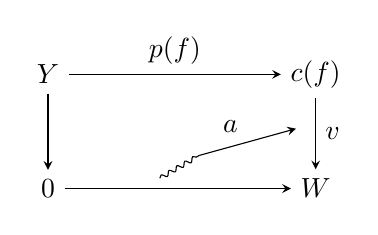
\begin{tikzpicture}[>=stealth,baseline=(current bounding box.center)]
    \node (Y)  at (0,1.45) {$Y$};
    \node (Cf) at (3.4,1.45) {$c(f)$};
    \node (Z)  at (0,0) {$0$};
    \node (W)  at (3.4,0) {$W$};
    \draw[->] (Y) -- node[above] {$p(f)$} (Cf);
    \draw[->] (Y) -- (Z);
    \draw[->] (Cf) -- node[right] {$v$} (W);
    \draw[->] (Z) -- (W);
    \draw[decorate,decoration={snake,amplitude=0.8pt,segment length=3.3pt}]
      (1.42,0.13) -- (1.92,0.42);
    \draw[->] (1.92,0.42) -- node[above left] {$a$} (3.15,0.76);
  \end{tikzpicture}
  \tag{3.2.9.5}
\end{equation}

\VerdierSemanticAnchor{ch1-3-2-9-n-morphism}
を得る。これは (3.1.3) により、三つ組
$\bigl(m\colon Y\longrightarrow W,\;a\colon0\rightsquigarrow m,\;
a\star f\colon0\rightsquigarrow mf\bigr)$ に対応する射
$n\colon c(p(f))\longrightarrow W$ を定める。射 $n$ が零にホモトピックである
ことを示すには、(3.1.5) により、図式 (3.2.9.5) が
$\operatorname{tr}_1(C)$ の零にホモトピックな射であることを示せばよい。
そのためには、$\beta\star p(f)=a$ を満たすホモトピー
$\beta\colon0\rightsquigarrow v$ の存在を示せばよい。射
$v\colon c(f)\longrightarrow W$ の成分は

\VerdierSemanticAnchor{ch1-3-2-9-eq6}
\begin{equation}
  v^i=(m^i,a^if^{i+1})\colon Y^i\oplus X^{i+1}\longrightarrow W^i
  \tag{3.2.9.6}
\end{equation}
であり、成分

\VerdierSemanticAnchor{ch1-3-2-9-eq7}
\begin{equation}
  \beta^i=(a^i,0)\colon Y^{i+1}\oplus X^{i+2}\longrightarrow W^i
  \tag{3.2.9.7}
\end{equation}

\VerdierSemanticAnchor{ch1-3-2-9-conclusion}
をもつホモトピー $\beta$ が $0$ と $v$ を結び、
$\beta\star p(f)=a$ を満たすことは直ちに確かめられる。これで主張
(3.2.7.3) の証明が完了する。

\VerdierSemanticAnchor{ch1-3-2-10}
\noindent\textbf{3.2.10. 主張 (3.2.7.4) の証明。}\quad
\VerdierSemanticAnchor{ch1-3-2-10-y1-represented-functor}
対象 $Y[1]$ は次の関手を表現する：

\VerdierSemanticAnchor{ch1-3-2-10-eq1}
\begin{equation}
  W\longmapsto
  \left\{\,
  \vcenter{\hbox{%
    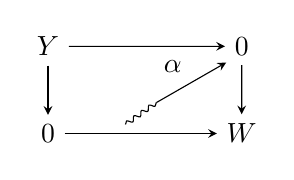
\begin{tikzpicture}[>=stealth,baseline=(current bounding box.center),scale=0.82,
      every node/.style={}]
      \node (Y) at (0,1.35) {$Y$};
      \node (ZT) at (3.0,1.35) {$0$};
      \node (ZB) at (0,0) {$0$};
      \node (W) at (3.0,0) {$W$};
      \draw[->] (Y) -- (ZT);
      \draw[->] (Y) -- (ZB);
      \draw[->] (ZT) -- (W);
      \draw[->] (ZB) -- (W);
      \draw[decorate,decoration={snake,amplitude=0.8pt,segment length=3.3pt}]
        (1.20,0.14) -- (1.68,0.48);
      \draw[->] (1.68,0.48) -- node[above left] {$\alpha$} (2.76,1.10);
    \end{tikzpicture}%
  }}\,\right\}.
  \tag{3.2.10.1}
\end{equation}

\VerdierSemanticAnchor{ch1-3-2-10-f1-functorial-map}
また、射 $f[1]\colon X[1]\longrightarrow Y[1]$ は次の関手の射を表現する：

\VerdierSemanticAnchor{ch1-3-2-10-eq2}
\begin{equation}
  \begin{gathered}
    D=
    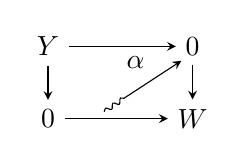
\begin{tikzpicture}[>=stealth,baseline=(current bounding box.center),scale=0.68,
      every node/.style={}]
      \node (Y) at (0,1.35) {$Y$};
      \node (ZT) at (2.7,1.35) {$0$};
      \node (ZB) at (0,0) {$0$};
      \node (W) at (2.7,0) {$W$};
      \draw[->] (Y) -- (ZT); \draw[->] (Y) -- (ZB);
      \draw[->] (ZT) -- (W); \draw[->] (ZB) -- (W);
      \draw[decorate,decoration={snake,amplitude=0.8pt,segment length=3.3pt}]
        (1.05,0.13) -- (1.48,0.42);
      \draw[->] (1.48,0.42) -- node[above left] {$\alpha$} (2.49,1.08);
    \end{tikzpicture}
    \quad\longmapsto\quad f[1]D=
    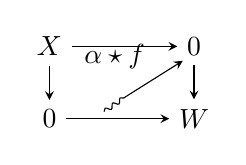
\begin{tikzpicture}[>=stealth,baseline=(current bounding box.center),scale=0.68,
      every node/.style={}]
      \node (X) at (0,1.35) {$X$};
      \node (ZT) at (2.7,1.35) {$0$};
      \node (ZB) at (0,0) {$0$};
      \node (W) at (2.7,0) {$W$};
      \draw[->] (X) -- (ZT); \draw[->] (X) -- (ZB);
      \draw[->] (ZT) -- (W); \draw[->] (ZB) -- (W);
      \draw[decorate,decoration={snake,amplitude=0.8pt,segment length=3.3pt}]
        (1.02,0.13) -- (1.44,0.42);
      \draw[->] (1.44,0.42) -- node[above left] {$\alpha\star f$} (2.49,1.08);
    \end{tikzpicture}
  \end{gathered}
  \tag{3.2.10.2}
\end{equation}%
\VerdierSourcePageContinue{0093}%
\begingroup
\setlength{\abovedisplayskip}{5pt plus 2pt minus 2pt}%
\setlength{\belowdisplayskip}{5pt plus 2pt minus 2pt}%
\VerdierSemanticAnchor{ch1-3-2-10-qpf-functorial-map}
同様に、射 $q(p(f))\colon c(p(f))\longrightarrow Y[1]$ は
次の関手の射を表現する：

\VerdierSemanticAnchor{ch1-3-2-10-eq3}
\begin{equation}
  \begin{gathered}
    D=
    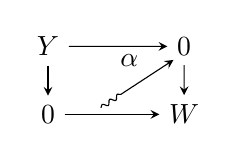
\begin{tikzpicture}[>=stealth,baseline=(current bounding box.center),scale=0.64,
      every node/.style={}]
      \node (Y) at (0,1.35) {$Y$};
      \node (ZT) at (2.7,1.35) {$0$};
      \node (ZB) at (0,0) {$0$};
      \node (W) at (2.7,0) {$W$};
      \draw[->] (Y) -- (ZT); \draw[->] (Y) -- (ZB);
      \draw[->] (ZT) -- (W); \draw[->] (ZB) -- (W);
      \draw[decorate,decoration={snake,amplitude=0.8pt,segment length=3.3pt}]
        (1.05,0.13) -- (1.48,0.42);
      \draw[->] (1.48,0.42) -- node[above left] {$\alpha$} (2.49,1.08);
    \end{tikzpicture}
    \quad\longmapsto\quad
    q(p(f))D=
    \bigl(0\colon Y\longrightarrow W,\;
      \alpha\colon0\rightsquigarrow0,\;
      0\colon0\rightsquigarrow0\bigr).
  \end{gathered}
  \tag{3.2.10.3}
\end{equation}

\VerdierSemanticAnchor{ch1-3-2-10-conclusion}
したがって、(3.2.8.4) を用いると、(3.2.7.4) を証明するには、任意の図式
\[
  D=
  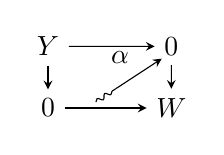
\begin{tikzpicture}[>=stealth,baseline=(current bounding box.center),scale=0.58,
    every node/.style={}]
    \node (Y) at (0,1.35) {$Y$};
    \node (ZT) at (2.7,1.35) {$0$};
    \node (ZB) at (0,0) {$0$};
    \node (W) at (2.7,0) {$W$};
    \draw[->] (Y) -- (ZT); \draw[->] (Y) -- (ZB);
    \draw[->] (ZT) -- (W); \draw[->] (ZB) -- (W);
    \draw[decorate,decoration={snake,amplitude=0.8pt,segment length=3.3pt}]
      (1.05,0.13) -- (1.48,0.42);
    \draw[->] (1.48,0.42) -- node[above left] {$\alpha$} (2.49,1.08);
  \end{tikzpicture}
  \qquad Hq(p(f))D+f[1]D=0.
\]
であることに注意すれば十分である。

\VerdierSemanticAnchor{ch1-3-2-11}
\noindent\textbf{3.2.11.}
\VerdierSemanticAnchor{ch1-3-2-11-composable-morphisms}
$X\xrightarrow{f}Y\xrightarrow{g}Z$ を $\operatorname{comp}(C)$ の二つの射
とする。$gf=h$ とおく。これらのデータから、二つの可換図式を構成できる：

\VerdierSemanticAnchor{ch1-3-2-11-eq1}
\begin{equation}
  \begin{gathered}
  D=
  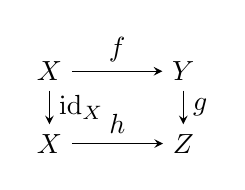
\begin{tikzpicture}[>=stealth,baseline=(current bounding box.center),scale=0.68,
    every node/.style={}]
    \node (X1) at (0,1.35) {$X$}; \node (Y) at (2.5,1.35) {$Y$};
    \node (X2) at (0,0) {$X$}; \node (Z) at (2.5,0) {$Z$};
    \draw[->] (X1) -- node[above] {$f$} (Y);
    \draw[->] (X1) -- node[right] {$\operatorname{id}_X$} (X2);
    \draw[->] (Y) -- node[right] {$g$} (Z);
    \draw[->] (X2) -- node[above] {$h$} (Z);
  \end{tikzpicture},
  \qquad
  D'=
  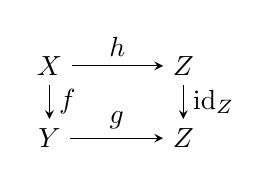
\begin{tikzpicture}[>=stealth,baseline=(current bounding box.center),scale=0.68,
    every node/.style={}]
    \node (X) at (0,1.35) {$X$}; \node (Z1) at (2.5,1.35) {$Z$};
    \node (Y) at (0,0) {$Y$}; \node (Z2) at (2.5,0) {$Z$};
    \draw[->] (X) -- node[above] {$h$} (Z1);
    \draw[->] (X) -- node[right] {$f$} (Y);
    \draw[->] (Z1) -- node[right] {$\operatorname{id}_Z$} (Z2);
    \draw[->] (Y) -- node[above] {$g$} (Z2);
  \end{tikzpicture}
  \end{gathered}
  \tag{3.2.11.1}
\end{equation}

\VerdierSemanticAnchor{ch1-3-2-11-cone-images}
これらを $\operatorname{tr}_1(C)$ の射と解釈する。したがって、写像錐関手を
適用すると二つの図式を得る：
\[
  c(f)\xrightarrow{c(D)}c(h)\xrightarrow{c(D')}c(g)
\]

\VerdierSemanticAnchor{ch1-3-2-11-eq2}
\begin{equation}
  I=
  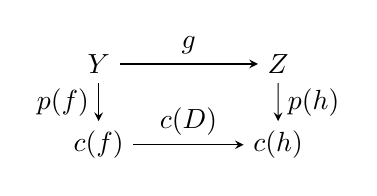
\begin{tikzpicture}[>=stealth,baseline=(current bounding box.center),scale=0.76,
    every node/.style={}]
    \node (Y) at (0,1.35) {$Y$}; \node (Z) at (3.0,1.35) {$Z$};
    \node (Cf) at (0,0) {$c(f)$}; \node (Ch) at (3.0,0) {$c(h)$};
    \draw[->] (Y) -- node[above] {$g$} (Z);
    \draw[->] (Y) -- node[left] {$p(f)$} (Cf);
    \draw[->] (Z) -- node[right] {$p(h)$} (Ch);
    \draw[->] (Cf) -- node[above] {$c(D)$} (Ch);
  \end{tikzpicture}
  \tag{3.2.11.2}
\end{equation}

\VerdierSemanticAnchor{ch1-3-2-11-ci-morphism}
この最後の図式は可換正方形 (3.2.2.4) であるから、
$\operatorname{tr}_1(C)$ の射と解釈できる。そこで写像錐関手をもう一度
適用すると、射

\VerdierSemanticAnchor{ch1-3-2-11-eq3}
\begin{equation}
  c(I)\colon c(g)\longrightarrow c(c(D)).
  \tag{3.2.11.3}
\end{equation}
を得る。
\endgroup

\VerdierSourcePageBlock{0094}%
\begingroup
\setlength{\abovedisplayskip}{4pt plus 2pt minus 2pt}%
\setlength{\belowdisplayskip}{4pt plus 2pt minus 2pt}%
\VerdierSemanticAnchor{ch1-3-2-12}
\noindent\textbf{命題 3.2.12.}\quad
\VerdierSemanticAnchor{ch1-3-2-12-a}
a) 射 $c(I)\colon c(g)\longrightarrow c(c(D))$ はホモトピー同値である。

\VerdierSemanticAnchor{ch1-3-2-12-b}
b) 図式

\VerdierSemanticAnchor{ch1-3-2-12-eq1}
\begin{equation}
  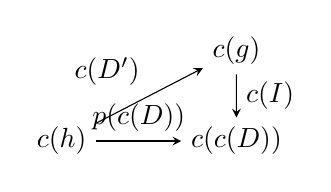
\begin{tikzpicture}[>=stealth,baseline=(current bounding box.center),scale=0.74,
    every node/.style={}]
    \node (Ch) at (0,0) {$c(h)$};
    \node (Cg) at (3.0,1.55) {$c(g)$};
    \node (CcD) at (3.0,0) {$c(c(D))$};
    \draw[->] (Ch) -- node[above left] {$c(D')$} (Cg);
    \draw[->] (Cg) -- node[right] {$c(I)$} (CcD);
    \draw[->] (Ch) -- node[above] {$p(c(D))$} (CcD);
  \end{tikzpicture}
  \tag{3.2.12.1}
\end{equation}
はホモトピーを除いて可換である。

\VerdierSemanticAnchor{ch1-3-2-12-c}
c) 図式

\VerdierSemanticAnchor{ch1-3-2-12-eq2}
\begin{equation}
  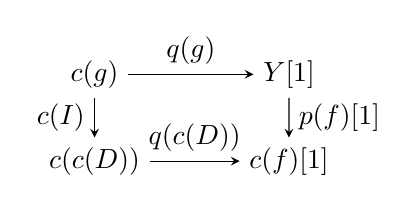
\begin{tikzpicture}[>=stealth,baseline=(current bounding box.center),scale=0.76,
    every node/.style={}]
    \node (Cg) at (0,1.45) {$c(g)$};
    \node (Y) at (3.25,1.45) {$Y[1]$};
    \node (CcD) at (0,0) {$c(c(D))$};
    \node (Cf) at (3.25,0) {$c(f)[1]$};
    \draw[->] (Cg) -- node[above] {$q(g)$} (Y);
    \draw[->] (Cg) -- node[left] {$c(I)$} (CcD);
    \draw[->] (Y) -- node[right] {$p(f)[1]$} (Cf);
    \draw[->] (CcD) -- node[above] {$q(c(D))$} (Cf);
  \end{tikzpicture}
  \tag{3.2.12.2}
\end{equation}
は可換である。

\VerdierSemanticAnchor{ch1-3-2-12-component-calculation}
実際、直接計算すれば、射 $c(I)$ の第 $i$ 成分は

\VerdierSemanticAnchor{ch1-3-2-12-eq3}
\begin{equation}
  c(I)^i=
  \begin{pmatrix}
    \operatorname{id}&0\\
    0&0\\
    0&\operatorname{id}\\
    0&0
  \end{pmatrix}
  \colon Z^i\oplus Y^{i+1}\longrightarrow
  Z^i\oplus X^{i+1}\oplus Y^{i+1}\oplus X^{i+2}.
  \tag{3.2.12.3}
\end{equation}
であることが分かる。

\VerdierSemanticAnchor{ch1-3-2-12-inverse}
射 $u\colon c(c(D))\longrightarrow c(g)$ の成分を

\VerdierSemanticAnchor{ch1-3-2-12-eq4}
\begin{equation}
  u^i=
  \begin{pmatrix}
    \operatorname{id}&0&0&0\\
    0&f^{i+1}&\operatorname{id}&0
  \end{pmatrix}
  \colon Z^i\oplus X^{i+1}\oplus Y^{i+1}\oplus X^{i+2}
  \longrightarrow Z^i\oplus Y^{i+1}
  \tag{3.2.12.4}
\end{equation}
と定めると、これはホモトピーを除いて $c(I)$ の逆であり、第一の主張が
証明される。第二の主張を証明するには、図式

\VerdierSemanticAnchor{ch1-3-2-12-eq5}
\begin{equation}
  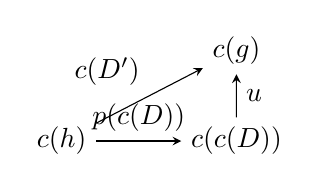
\begin{tikzpicture}[>=stealth,baseline=(current bounding box.center),scale=0.74,
    every node/.style={}]
    \node (Ch) at (0,0) {$c(h)$};
    \node (Cg) at (3.0,1.55) {$c(g)$};
    \node (CcD) at (3.0,0) {$c(c(D))$};
    \draw[->] (Ch) -- node[above left] {$c(D')$} (Cg);
    \draw[->] (CcD) -- node[right] {$u$} (Cg);
    \draw[->] (Ch) -- node[above] {$p(c(D))$} (CcD);
  \end{tikzpicture}
  \tag{3.2.12.5}
\end{equation}

\VerdierSemanticAnchor{ch1-3-2-12-conclusion}
が可換であることを確かめればよく、これは成分を明示すれば分かる。最後に、
(3.2.2) により、射 $q(f)$ の関手性 (3.2.2.2) から正方形
(3.2.12.2) が可換であることが従う。
\endgroup

\VerdierSourcePageBlock{0095}%
\begingroup
\setlength{\abovedisplayskip}{4pt plus 2pt minus 2pt}%
\setlength{\belowdisplayskip}{4pt plus 2pt minus 2pt}%
\VerdierSemanticAnchor{ch1-3-3}
\subsection{完全三角の性質}

\VerdierSemanticAnchor{ch1-3-3-1}
\noindent\textbf{定義 3.3.1.}\quad
\VerdierSemanticAnchor{ch1-3-3-1-distinguished-triangle}
$K(C)$ の三角
$X\xrightarrow{u}Y\xrightarrow{v}Z\xrightarrow{w}X[1]$ が
\emph{完全三角}であるとは、$\operatorname{Tr}_1(C)$ の対象
$X'\xrightarrow{\dot f'}Y'$ と三角の同型（(3.2.1.3) および
(3.2.2.7)）

\VerdierSemanticAnchor{ch1-3-3-1-isomorphism-diagram}
\begin{center}
  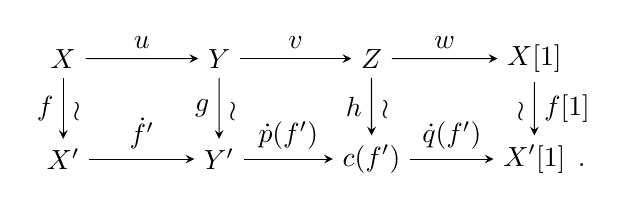
\begin{tikzpicture}[>=stealth,scale=0.88,every node/.style={}]
    \node (X)   at (0,1.45) {$X$};
    \node (Y)   at (2.25,1.45) {$Y$};
    \node (Z)   at (4.45,1.45) {$Z$};
    \node (Xs)  at (6.80,1.45) {$X[1]$};
    \node (Xp)  at (0,0) {$X'$};
    \node (Yp)  at (2.25,0) {$Y'$};
    \node (Cf)  at (4.45,0) {$c(f')$};
    \node (Xps) at (6.80,0) {$X'[1]$};
    \node[anchor=base west,inner sep=0pt,xshift=.08em] at (Xps.base east) {$.$};
    \draw[->] (X) -- node[above] {$u$} (Y);
    \draw[->] (Y) -- node[above] {$v$} (Z);
    \draw[->] (Z) -- node[above] {$w$} (Xs);
    \draw[->] (Xp) -- node[above] {$\dot f'$} (Yp);
    \draw[->] (Yp) -- node[above] {$\dot p(f')$} (Cf);
    \draw[->] (Cf) -- node[above] {$\dot q(f')$} (Xps);
    \draw[->] (X) -- node[left] {$f$} node[right,pos=.55] {$\wr$} (Xp);
    \draw[->] (Y) -- node[left] {$g$} node[right,pos=.55] {$\wr$} (Yp);
    \draw[->] (Z) -- node[left] {$h$} node[right,pos=.55] {$\wr$} (Cf);
    \draw[->] (Xs) -- node[right] {$f[1]$} node[left,pos=.55] {$\wr$} (Xps);
  \end{tikzpicture}
\end{center}
が存在することをいう。

\VerdierSemanticAnchor{ch1-3-3-2}
\noindent\textbf{命題 3.3.2. (TRI)}\quad
\VerdierSemanticAnchor{ch1-3-3-2-isomorphism-invariance}
\textit{$K(C)$ の三角で完全三角に同型なものは、すべて完全三角である。}
\VerdierSemanticAnchor{ch1-3-3-2-identity-triangle}
\textit{$K(C)$ の任意の対象 $X$ に対し、三角
$X\xrightarrow{\operatorname{id}_X}X\longrightarrow0\longrightarrow X[1]$
は完全三角である。}
\VerdierSemanticAnchor{ch1-3-3-2-completion}
\textit{$K(C)$ の任意の射 $u\colon X\to Y$ は、完全三角
$X\xrightarrow{u}Y\xrightarrow{v}Z\xrightarrow{w}X[1]$ に含まれる。}

\VerdierSemanticAnchor{ch1-3-3-2-proof-first}
第一の主張は自明である。第二の主張を証明するには、図式

\VerdierSemanticAnchor{ch1-3-3-2-identity-comparison}
\begin{center}
  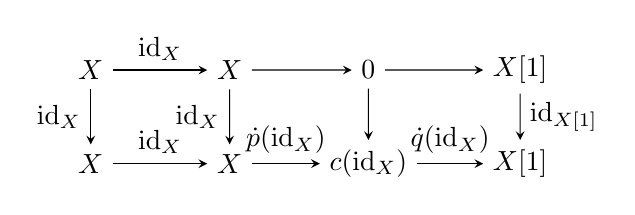
\begin{tikzpicture}[>=stealth,scale=0.82,every node/.style={}]
    \node (X1) at (0,1.45) {$X$};
    \node (X2) at (2.15,1.45) {$X$};
    \node (Z1) at (4.30,1.45) {$0$};
    \node (Xs1) at (6.65,1.45) {$X[1]$};
    \node (X3) at (0,0) {$X$};
    \node (X4) at (2.15,0) {$X$};
    \node (Cid) at (4.30,0) {$c(\operatorname{id}_X)$};
    \node (Xs2) at (6.65,0) {$X[1]$};
    \draw[->] (X1) -- node[above] {$\operatorname{id}_X$} (X2);
    \draw[->] (X2) -- (Z1);
    \draw[->] (Z1) -- (Xs1);
    \draw[->] (X3) -- node[above] {$\operatorname{id}_X$} (X4);
    \draw[->] (X4) -- node[above] {$\dot p(\operatorname{id}_X)$} (Cid);
    \draw[->] (Cid) -- node[above] {$\dot q(\operatorname{id}_X)$} (Xs2);
    \draw[->] (X1) -- node[left] {$\operatorname{id}_X$} (X3);
    \draw[->] (X2) -- node[left] {$\operatorname{id}_X$} (X4);
    \draw[->] (Z1) -- (Cid);
    \draw[->] (Xs1) -- node[right] {$\operatorname{id}_{X[1]}$} (Xs2);
  \end{tikzpicture}
\end{center}

\VerdierSemanticAnchor{ch1-3-3-2-identity-cone-null}
が $K(C)$ における三角の同型であることを示せばよい。したがって、
$c(\operatorname{id}_X)$ が零とホモトピックであることを示せば十分である。
ところで、$\operatorname{tr}_1(C)$ におけるホモトピーの定義 (3.1.4) から、
次の形の $\operatorname{tr}_1(C)$ の任意の射

\VerdierSemanticAnchor{ch1-3-3-2-tr1-null-diagram}
\begin{center}
  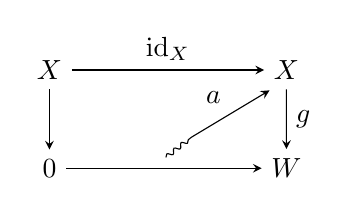
\begin{tikzpicture}[>=stealth,scale=0.86,every node/.style={}]
    \node (X1) at (0,1.45) {$X$};
    \node (X2) at (3.50,1.45) {$X$};
    \node (Z)  at (0,0) {$0$};
    \node (W)  at (3.50,0) {$W$};
    \draw[->] (X1) -- node[above] {$\operatorname{id}_X$} (X2);
    \draw[->] (X1) -- (Z);
    \draw[->] (X2) -- node[right] {$g$} (W);
    \draw[->] (Z) -- (W);
    \draw[decorate,decoration={snake,amplitude=0.8pt,segment length=3.3pt}]
      (1.72,0.16) -- (2.10,0.46);
    \draw[->] (2.10,0.46) -- node[above left] {$a$} (3.25,1.15);
  \end{tikzpicture}
\end{center}

\VerdierSemanticAnchor{ch1-3-3-2-tr1-null-conclusion}
は零とホモトピックであることが直ちに従う。
\VerdierSemanticAnchor{ch1-3-3-2-adjunction}
このとき錐関手の随伴性 (3.1.6) から、
$c(\operatorname{id}_X)$ が零とホモトピックであることが分かる。
\VerdierSemanticAnchor{ch1-3-3-2-open-morphism}
$f\colon X\to Y$ を射とする
\endgroup%
\VerdierSourcePageContinue{0096}%
\begingroup
\setlength{\abovedisplayskip}{3pt plus 2pt minus 2pt}%
\setlength{\belowdisplayskip}{3pt plus 2pt minus 2pt}%
\VerdierSemanticAnchor{ch1-3-3-2-open-morphism-continuation}
これは $\operatorname{comp}(C)$ において
$u\colon X\to Y$ のホモトピー類に属するものとする。
\VerdierSemanticAnchor{ch1-3-3-2-representative}
すると $\operatorname{Tr}_1(C)$ の対象
$X\xrightarrow{\dot f}Y$ が得られる。
\VerdierSemanticAnchor{ch1-3-3-2-completion-cone}
完全三角
\begin{equation*}
  X\xrightarrow{u}Y\xrightarrow{\dot p(f)}c(f)
  \xrightarrow{\dot q(f)}X[1]
\end{equation*}
\VerdierSemanticAnchor{ch1-3-3-2-completion-conclusion}
は射 $u$ を含む。

\VerdierSemanticAnchor{ch1-3-3-3}
\noindent\textbf{命題 3.3.3. (TRII)}\quad
\VerdierSemanticAnchor{ch1-3-3-3-trii}
\textit{$K(C)$ の三角
$X\xrightarrow{u}Y\xrightarrow{v}Z\xrightarrow{w}X[1]$ が完全三角である
ための必要十分条件は、三角
$Y\xrightarrow{v}Z\xrightarrow{w}X[1]\xrightarrow{-u[1]}Y[1]$
が完全三角であることである。}

\VerdierSemanticAnchor{ch1-3-3-3-proof-forward}
三角 $X\xrightarrow{u}Y\xrightarrow{v}Z\xrightarrow{w}X[1]$ が
完全三角であると仮定する。このとき、これは次の形の三角に同型である：

\VerdierSemanticAnchor{ch1-3-3-3-cone-model}
\begin{equation*}
  X'\xrightarrow{\dot f}Y'\xrightarrow{\dot p(f)}c(f)
  \xrightarrow{\dot q(f)}X'[1],
\end{equation*}
ここで $X'\xrightarrow{\dot f}Y'$ は $\operatorname{Tr}_1(C)$ の対象である。
したがって、三角

\VerdierSemanticAnchor{ch1-3-3-3-rotated-model}
\begin{equation*}
  Y'\xrightarrow{\dot p(f)}c(f)\xrightarrow{\dot q(f)}X'[1]
  \xrightarrow{-\dot f[1]}Y'[1],
\end{equation*}
が完全三角であることを示せばよい。(3.2.6) により、図式

\VerdierSemanticAnchor{ch1-3-3-3-comparison}
\begin{center}
  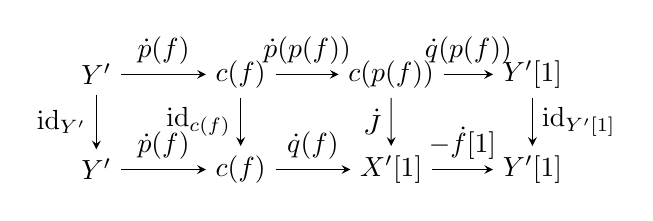
\begin{tikzpicture}[>=stealth,scale=0.78,every node/.style={}]
    \node (Y1)  at (0,1.55) {$Y'$};
    \node (Cf1) at (2.35,1.55) {$c(f)$};
    \node (Cpf) at (4.80,1.55) {$c(p(f))$};
    \node (Ys1) at (7.10,1.55) {$Y'[1]$};
    \node (Y2)  at (0,0) {$Y'$};
    \node (Cf2) at (2.35,0) {$c(f)$};
    \node (Xs)  at (4.80,0) {$X'[1]$};
    \node (Ys2) at (7.10,0) {$Y'[1]$};
    \draw[->] (Y1) -- node[above] {$\dot p(f)$} (Cf1);
    \draw[->] (Cf1) -- node[above] {$\dot p(p(f))$} (Cpf);
    \draw[->] (Cpf) -- node[above] {$\dot q(p(f))$} (Ys1);
    \draw[->] (Y2) -- node[above] {$\dot p(f)$} (Cf2);
    \draw[->] (Cf2) -- node[above] {$\dot q(f)$} (Xs);
    \draw[->] (Xs) -- node[above] {$-\dot f[1]$} (Ys2);
    \draw[->] (Y1) -- node[left] {$\operatorname{id}_{Y'}$} (Y2);
    \draw[->] (Cf1) -- node[left] {$\operatorname{id}_{c(f)}$} (Cf2);
    \draw[->] (Cpf) -- node[left] {$\dot J$} (Xs);
    \draw[->] (Ys1) -- node[right] {$\operatorname{id}_{Y'[1]}$} (Ys2);
  \end{tikzpicture}
\end{center}

\VerdierSemanticAnchor{ch1-3-3-3-forward-conclusion}
は $K(C)$ における三角の同型である。

\VerdierSemanticAnchor{ch1-3-3-3-proof-reverse}
次に、三角
$Y\xrightarrow{v}Z\xrightarrow{w}X[1]\xrightarrow{-u[1]}Y[1]$ が
完全三角であると仮定する。(3.2.4) から、三角

\VerdierSemanticAnchor{ch1-3-3-3-shifted-triangle}
\begin{equation*}
  Y[-1]\xrightarrow{v[-1]}Z[-1]\xrightarrow{w[-1]}X
  \xrightarrow{u}Y
\end{equation*}
は完全三角であり、さらに、
\VerdierSemanticAnchor{ch1-3-3-3-double-rotation}
先の議論を二度適用すれば、三角
\begin{equation*}
  X\xrightarrow{u}Y\xrightarrow{v}Z\xrightarrow{w}X[1]
\end{equation*}
\VerdierSemanticAnchor{ch1-3-3-3-conclusion}
も完全三角であることが従う。これで証明が完了する。
\endgroup

\VerdierSourcePageBlock{0097}%
\begingroup
\setlength{\abovedisplayskip}{3pt plus 2pt minus 2pt}%
\setlength{\belowdisplayskip}{3pt plus 2pt minus 2pt}%
\setlength{\jot}{2pt}%
\VerdierSemanticAnchor{ch1-3-3-4}
\noindent\textbf{命題 3.3.4. (TRIII)}\quad
\begingroup\itshape
\VerdierSemanticAnchor{ch1-3-3-4-triii}
$K(C)$ の二つの完全三角

\VerdierSemanticAnchor{ch1-3-3-4-source-triangles}
\begin{equation*}
  X\xrightarrow{u}Y\xrightarrow{v}Z\xrightarrow{w}X[1],
  \qquad
  X'\xrightarrow{u'}Y'\xrightarrow{v'}Z'\xrightarrow{w'}X'[1]
\end{equation*}
と、$K(C)$ における可換正方形

\VerdierSemanticAnchor{ch1-3-3-4-eq1}
\begin{equation}
  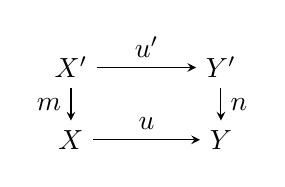
\begin{tikzpicture}[>=stealth,baseline=(current bounding box.center),scale=0.68,
    every node/.style={}]
    \node (Xp) at (0,1.35) {$X'$}; \node (Yp) at (2.8,1.35) {$Y'$};
    \node (X)  at (0,0) {$X$};   \node (Y)  at (2.8,0) {$Y$};
    \draw[->] (Xp) -- node[above] {$u'$} (Yp);
    \draw[->] (Xp) -- node[left] {$m$} (X);
    \draw[->] (Yp) -- node[right] {$n$} (Y);
    \draw[->] (X) -- node[above] {$u$} (Y);
  \end{tikzpicture}
  \tag{3.3.4.1}
\end{equation}
を考える。
\VerdierSemanticAnchor{ch1-3-3-4-filler}
図式

\VerdierSemanticAnchor{ch1-3-3-4-morphism-diagram}
\begin{center}
  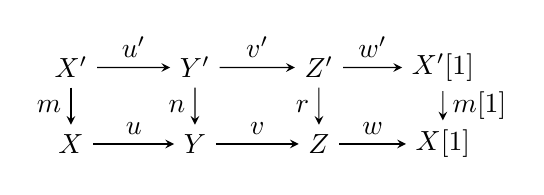
\begin{tikzpicture}[>=stealth,scale=0.67,every node/.style={}]
    \node (Xp)  at (0,1.45) {$X'$};
    \node (Yp)  at (2.35,1.45) {$Y'$};
    \node (Zp)  at (4.70,1.45) {$Z'$};
    \node (Xps) at (7.05,1.45) {$X'[1]$};
    \node (X)   at (0,0) {$X$};
    \node (Y)   at (2.35,0) {$Y$};
    \node (Z)   at (4.70,0) {$Z$};
    \node (Xs)  at (7.05,0) {$X[1]$};
    \draw[->] (Xp) -- node[above] {$u'$} (Yp);
    \draw[->] (Yp) -- node[above] {$v'$} (Zp);
    \draw[->] (Zp) -- node[above] {$w'$} (Xps);
    \draw[->] (X) -- node[above] {$u$} (Y);
    \draw[->] (Y) -- node[above] {$v$} (Z);
    \draw[->] (Z) -- node[above] {$w$} (Xs);
    \draw[->] (Xp) -- node[left] {$m$} (X);
    \draw[->] (Yp) -- node[left] {$n$} (Y);
    \draw[->] (Zp) -- node[left] {$r$} (Z);
    \draw[->] (Xps) -- node[right] {$m[1]$} (Xs);
  \end{tikzpicture}
\end{center}
\VerdierSemanticAnchor{ch1-3-3-4-morphism-conclusion}
が三角の射となるような射 $r\colon Z'\longrightarrow Z$ が存在する。
\endgroup

\VerdierSemanticAnchor{ch1-3-3-4-proof}
定義により、与えられた三角は次の形の三角に同型である：

\VerdierSemanticAnchor{ch1-3-3-4-cone-models}
\begin{align*}
  V&\xrightarrow{\dot f}W\xrightarrow{\dot p(f)}c(f)
     \xrightarrow{\dot q(f)}V[1],\\
  V'&\xrightarrow{\dot f'}W'\xrightarrow{\dot p(f')}c(f')
     \xrightarrow{\dot q(f')}V'[1],
\end{align*}
\VerdierSemanticAnchor{ch1-3-3-4-square-reduction}
したがって、正方形 (3.3.4.1) は次の正方形に同型である：

\VerdierSemanticAnchor{ch1-3-3-4-homotopy-class-square}
\begin{center}
  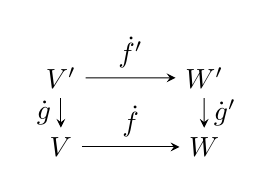
\begin{tikzpicture}[>=stealth,scale=0.65,every node/.style={}]
    \node (Vp) at (0,1.35) {$V'$}; \node (Wp) at (2.8,1.35) {$W'$};
    \node (V)  at (0,0) {$V$};   \node (W)  at (2.8,0) {$W$};
    \draw[->] (Vp) -- node[above] {$\dot f'$} (Wp);
    \draw[->] (Vp) -- node[left] {$\dot g$} (V);
    \draw[->] (Wp) -- node[right] {$\dot g'$} (W);
    \draw[->] (V) -- node[above] {$\dot f$} (W);
  \end{tikzpicture},
\end{center}
\VerdierSemanticAnchor{ch1-3-3-4-representatives}
ここで $g\colon V'\longrightarrow V$ と $g'\colon W'\longrightarrow W$ は
$\operatorname{comp}(C)$ の射である。$\operatorname{comp}(C)$ における正方形

\VerdierSemanticAnchor{ch1-3-3-4-comp-square}
\begin{center}
  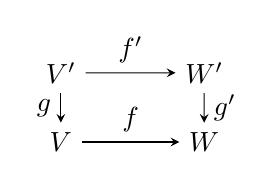
\begin{tikzpicture}[>=stealth,scale=0.65,every node/.style={}]
    \node (Vp) at (0,1.35) {$V'$}; \node (Wp) at (2.8,1.35) {$W'$};
    \node (V)  at (0,0) {$V$};   \node (W)  at (2.8,0) {$W$};
    \draw[->] (Vp) -- node[above] {$f'$} (Wp);
    \draw[->] (Vp) -- node[left] {$g$} (V);
    \draw[->] (Wp) -- node[right] {$g'$} (W);
    \draw[->] (V) -- node[above] {$f$} (W);
  \end{tikzpicture}
\end{center}
\VerdierSemanticAnchor{ch1-3-3-4-open-conclusion}
\endgroup%
\VerdierSourcePageContinue{0098}%
\begingroup
\setlength{\abovedisplayskip}{3pt plus 2pt minus 2pt}%
\setlength{\belowdisplayskip}{3pt plus 2pt minus 2pt}%
\setlength{\jot}{2pt}%
\VerdierSemanticAnchor{ch1-3-3-4-open-conclusion-continuation}
はホモトピーを除いて可換である。
\VerdierSemanticAnchor{ch1-3-3-4-homotopy}
ホモトピー $a\colon fg\rightsquigarrow g'f'$ を取る。図式

\VerdierSemanticAnchor{ch1-3-3-4-tr1-morphism}
\begin{center}
  $D={}$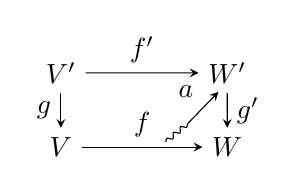
\begin{tikzpicture}[>=stealth,baseline=(current bounding box.center),
    scale=0.65,every node/.style={}]
    \node (Vp) at (0,1.45) {$V'$}; \node (Wp) at (3.25,1.45) {$W'$};
    \node (V)  at (0,0) {$V$};   \node (W)  at (3.25,0) {$W$};
    \draw[->] (Vp) -- node[above] {$f'$} (Wp);
    \draw[->] (Vp) -- node[left] {$g$} (V);
    \draw[->] (Wp) -- node[right] {$g'$} (W);
    \draw[->] (V) -- node[above] {$f$} (W);
    \draw[decorate,decoration={snake,amplitude=0.8pt,segment length=3.3pt}]
      (2.05,0.10) -- (2.48,0.46);
    \draw[->] (2.48,0.46) -- node[above left] {$a$} (3.08,1.08);
  \end{tikzpicture}
\end{center}
は $\operatorname{tr}_1(C)$ の射である。(3.2.2.7) から、図式

\VerdierSemanticAnchor{ch1-3-3-4-cone-morphism-diagram}
\begin{center}
  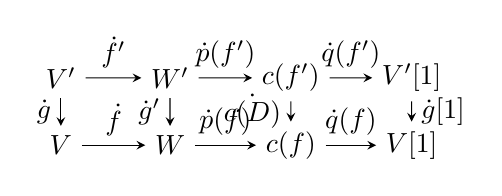
\begin{tikzpicture}[>=stealth,scale=0.59,every node/.style={}]
    \node (Vp)  at (0,1.45) {$V'$};
    \node (Wp)  at (2.35,1.45) {$W'$};
    \node (Cfp) at (4.95,1.45) {$c(f')$};
    \node (Vps) at (7.55,1.45) {$V'[1]$};
    \node (V)   at (0,0) {$V$};
    \node (W)   at (2.35,0) {$W$};
    \node (Cf)  at (4.95,0) {$c(f)$};
    \node (Vs)  at (7.55,0) {$V[1]$};
    \draw[->] (Vp) -- node[above] {$\dot f'$} (Wp);
    \draw[->] (Wp) -- node[above] {$\dot p(f')$} (Cfp);
    \draw[->] (Cfp) -- node[above] {$\dot q(f')$} (Vps);
    \draw[->] (V) -- node[above] {$\dot f$} (W);
    \draw[->] (W) -- node[above] {$\dot p(f)$} (Cf);
    \draw[->] (Cf) -- node[above] {$\dot q(f)$} (Vs);
    \draw[->] (Vp) -- node[left] {$\dot g$} (V);
    \draw[->] (Wp) -- node[left] {$\dot g'$} (W);
    \draw[->] (Cfp) -- node[left] {$\dot{c(D)}$} (Cf);
    \draw[->] (Vps) -- node[right] {$\dot g[1]$} (Vs);
  \end{tikzpicture}
\end{center}
は $K(C)$ における三角の射である。したがって、射

\VerdierSemanticAnchor{ch1-3-3-4-r-conclusion}
\[
  r\colon Z'\longrightarrow Z.
\]
が存在する。

\VerdierSemanticAnchor{ch1-3-3-5}
\noindent\textbf{命題 3.3.5. (TRIV)}\quad
\begingroup\itshape
\VerdierSemanticAnchor{ch1-3-3-5-triv}
$K(C)$ における可換図式

\VerdierSemanticAnchor{ch1-3-3-5-input-triangle}
\begin{center}
  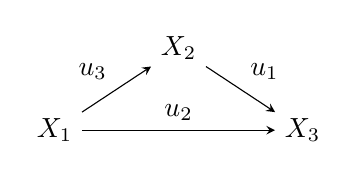
\begin{tikzpicture}[>=stealth,scale=0.67,every node/.style={}]
    \node (X1) at (0,0) {$X_1$};
    \node (X2) at (2.35,1.55) {$X_2$};
    \node (X3) at (4.70,0) {$X_3$};
    \draw[->] (X1) -- node[above left] {$u_3$} (X2);
    \draw[->] (X2) -- node[above right] {$u_1$} (X3);
    \draw[->] (X1) -- node[above] {$u_2$} (X3);
  \end{tikzpicture}
\end{center}
を考える。三つの完全三角

\VerdierSemanticAnchor{ch1-3-3-5-triangle-3}
\[
  X_1\xrightarrow{u_3}X_2\xrightarrow{v_3}Z_3
  \xrightarrow{w_3}X_1[1],
\]
\VerdierSemanticAnchor{ch1-3-3-5-triangle-1}
\[
  X_2\xrightarrow{u_1}X_3\xrightarrow{v_1}Z_1
  \xrightarrow{w_1}X_2[1],
\]
\VerdierSemanticAnchor{ch1-3-3-5-triangle-2}
\[
  X_1\xrightarrow{u_2}X_3\xrightarrow{v_2}Z_2
  \xrightarrow{w_2}X_1[1]
\]
\VerdierSemanticAnchor{ch1-3-3-5-morphisms}
および二つの射
\VerdierSemanticAnchor{ch1-3-3-5-m1}
\[
  m_1\colon Z_3\longrightarrow Z_2,
\]
\VerdierSemanticAnchor{ch1-3-3-5-m3}
\[
  m_3\colon Z_2\longrightarrow Z_1,
\]
\VerdierSemanticAnchor{ch1-3-3-5-open-conditions}
が存在して、次を満たす：
\endgroup
\endgroup%
\VerdierSourcePageContinue{0099}%
\begingroup
\setlength{\abovedisplayskip}{3pt plus 2pt minus 2pt}%
\setlength{\belowdisplayskip}{3pt plus 2pt minus 2pt}%
\setlength{\jot}{2pt}%
\VerdierSemanticAnchor{ch1-3-3-5-condition-a}
\noindent\textit{a) 図式}

\VerdierSemanticAnchor{ch1-3-3-5-morphism-triangles-first}
\begin{center}
  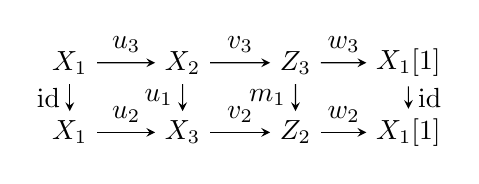
\begin{tikzpicture}[>=stealth,scale=0.61,every node/.style={}]
    \node (X1t) at (0,1.45) {$X_1$};
    \node (X2t) at (2.35,1.45) {$X_2$};
    \node (Z3t) at (4.70,1.45) {$Z_3$};
    \node (X1st) at (7.05,1.45) {$X_1[1]$};
    \node (X1b) at (0,0) {$X_1$};
    \node (X3b) at (2.35,0) {$X_3$};
    \node (Z2b) at (4.70,0) {$Z_2$};
    \node (X1sb) at (7.05,0) {$X_1[1]$};
    \draw[->] (X1t) -- node[above] {$u_3$} (X2t);
    \draw[->] (X2t) -- node[above] {$v_3$} (Z3t);
    \draw[->] (Z3t) -- node[above] {$w_3$} (X1st);
    \draw[->] (X1b) -- node[above] {$u_2$} (X3b);
    \draw[->] (X3b) -- node[above] {$v_2$} (Z2b);
    \draw[->] (Z2b) -- node[above] {$w_2$} (X1sb);
    \draw[->] (X1t) -- node[left] {$\mathrm{id}$} (X1b);
    \draw[->] (X2t) -- node[left] {$u_1$} (X3b);
    \draw[->] (Z3t) -- node[left] {$m_1$} (Z2b);
    \draw[->] (X1st) -- node[right] {$\mathrm{id}$} (X1sb);
  \end{tikzpicture}
\end{center}
\VerdierSemanticAnchor{ch1-3-3-5-morphism-triangles-second}
\begin{center}
  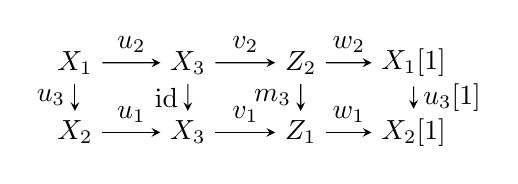
\begin{tikzpicture}[>=stealth,scale=0.61,every node/.style={}]
    \node (X1t) at (0,1.45) {$X_1$};
    \node (X3t) at (2.35,1.45) {$X_3$};
    \node (Z2t) at (4.70,1.45) {$Z_2$};
    \node (X1st) at (7.05,1.45) {$X_1[1]$};
    \node (X2b) at (0,0) {$X_2$};
    \node (X3b) at (2.35,0) {$X_3$};
    \node (Z1b) at (4.70,0) {$Z_1$};
    \node (X2sb) at (7.05,0) {$X_2[1]$};
    \draw[->] (X1t) -- node[above] {$u_2$} (X3t);
    \draw[->] (X3t) -- node[above] {$v_2$} (Z2t);
    \draw[->] (Z2t) -- node[above] {$w_2$} (X1st);
    \draw[->] (X2b) -- node[above] {$u_1$} (X3b);
    \draw[->] (X3b) -- node[above] {$v_1$} (Z1b);
    \draw[->] (Z1b) -- node[above] {$w_1$} (X2sb);
    \draw[->] (X1t) -- node[left] {$u_3$} (X2b);
    \draw[->] (X3t) -- node[left] {$\mathrm{id}$} (X3b);
    \draw[->] (Z2t) -- node[left] {$m_3$} (Z1b);
    \draw[->] (X1st) -- node[right] {$u_3[1]$} (X2sb);
  \end{tikzpicture}
\end{center}
\VerdierSemanticAnchor{ch1-3-3-5-condition-a-conclusion}
\textit{が三角の射である。}

\VerdierSemanticAnchor{ch1-3-3-5-condition-b}
\noindent\textit{b) 三角}
\VerdierSemanticAnchor{ch1-3-3-5-z-triangle}
\[
  Z_3\xrightarrow{m_1}Z_2\xrightarrow{m_3}Z_1
  \xrightarrow{v_3[1]w_1}Z_3[1]
\]
\VerdierSemanticAnchor{ch1-3-3-5-condition-b-conclusion}
\textit{が完全三角である。}

\VerdierSemanticAnchor{ch1-3-3-5-proof}
$\operatorname{comp}(C)$ の射
$f\colon X_1\longrightarrow X_2$（それぞれ
$g\colon X_2\longrightarrow X_3$）を、類 $\dot u_3$
（それぞれ $\dot u_1$）に属するものとして取る。
\VerdierSemanticAnchor{ch1-3-3-5-composite}
$h=gf\colon X_1\longrightarrow X_3$ とおく。射 $h$ は類
$\dot u_2$ に属する。命題を証明するには、完全三角として
(3.2.2) の三角

\VerdierSemanticAnchor{ch1-3-3-5-cone-triangles}
\begin{align*}
  X_1&\xrightarrow{\dot f}X_2\xrightarrow{\dot p(f)}c(f)
       \xrightarrow{\dot q(f)}X_1[1],\\
  X_2&\xrightarrow{\dot g}X_3\xrightarrow{\dot p(g)}c(g)
       \xrightarrow{\dot q(g)}X_2[1],\\
  X_1&\xrightarrow{\dot h}X_3\xrightarrow{\dot p(h)}c(h)
       \xrightarrow{\dot q(h)}X_1[1]
\end{align*}
\VerdierSemanticAnchor{ch1-3-3-5-cone-morphisms}
を取り、射として
\[
  c(D)\colon c(f)\longrightarrow c(h),
  \qquad
  c(D')\colon c(h)\longrightarrow c(g),
\]
を取れば十分である。ここで $D$ と $D'$ は図式

\VerdierSemanticAnchor{ch1-3-3-5-d-squares}
\begin{center}
  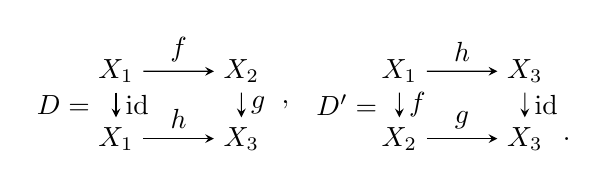
\begin{tikzpicture}[>=stealth,scale=0.59,every node/.style={}]
    \node at (-1.05,0.73) {$D={}$};
    \node (X1t) at (0,1.45) {$X_1$}; \node (X2t) at (2.70,1.45) {$X_2$};
    \node (X1b) at (0,0) {$X_1$};    \node (X3b) at (2.70,0) {$X_3$};
    \draw[->] (X1t) -- node[above] {$f$} (X2t);
    \draw[->] (X1t) -- node[right] {$\mathrm{id}$} (X1b);
    \draw[->] (X2t) -- node[right] {$g$} (X3b);
    \draw[->] (X1b) -- node[above] {$h$} (X3b);
    \node at (3.65,0.73) {$,$};
    \node at (5.05,0.73) {$D'={}$};
    \node (Y1t) at (6.10,1.45) {$X_1$}; \node (Y3t) at (8.80,1.45) {$X_3$};
    \node (Y2b) at (6.10,0) {$X_2$};    \node (Y3b) at (8.80,0) {$X_3$};
    \draw[->] (Y1t) -- node[above] {$h$} (Y3t);
    \draw[->] (Y1t) -- node[right] {$f$} (Y2b);
    \draw[->] (Y3t) -- node[right] {$\mathrm{id}$} (Y3b);
    \draw[->] (Y2b) -- node[above] {$g$} (Y3b);
    \node at (9.70,0.00) {$.$};
  \end{tikzpicture}
\end{center}
である。
\endgroup

\VerdierSourcePageBlock{0100}%
\begingroup
\VerdierSemanticAnchor{ch1-3-3-5-proof-completion}
実際、第一の主張は (3.2.2) の直接の帰結であり、命題 (3.2.12) により、射
$c(I)\colon c(g)\longrightarrow c(c(D))$ が存在して、図式

\VerdierSemanticAnchor{ch1-3-3-5-isomorphism-diagram}
\begin{center}
  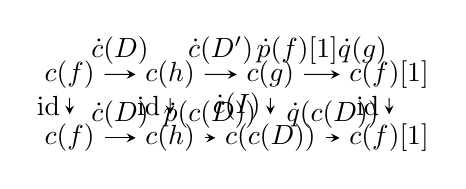
\begin{tikzpicture}[>=stealth,scale=0.52,every node/.style={}]
    \node (cf1) at (0,1.55) {$c(f)$};
    \node (ch1) at (2.45,1.55) {$c(h)$};
    \node (cg1) at (4.90,1.55) {$c(g)$};
    \node (cfs1) at (7.80,1.55) {$c(f)[1]$};
    \node (cf2) at (0,0) {$c(f)$};
    \node (ch2) at (2.45,0) {$c(h)$};
    \node (ccd) at (4.90,0) {$c(c(D))$};
    \node (cfs2) at (7.80,0) {$c(f)[1]$};
    \draw[->] (cf1) -- node[above] {$\dot c(D)$} (ch1);
    \draw[->] (ch1) -- node[above] {$\dot c(D')$} (cg1);
    \draw[->] (cg1) -- node[above] {$\dot p(f)[1]\dot q(g)$} (cfs1);
    \draw[->] (cf2) -- node[above] {$\dot c(D)$} (ch2);
    \draw[->] (ch2) -- node[above] {$\dot p(c(D))$} (ccd);
    \draw[->] (ccd) -- node[above] {$\dot q(c(D))$} (cfs2);
    \draw[->] (cf1) -- node[left] {$\mathrm{id}$} (cf2);
    \draw[->] (ch1) -- node[left] {$\mathrm{id}$} (ch2);
    \draw[->] (cg1) -- node[left] {$\dot c(I)$} (ccd);
    \draw[->] (cfs1) -- node[left] {$\mathrm{id}$} (cfs2);
  \end{tikzpicture}
\end{center}
\VerdierSemanticAnchor{ch1-3-3-5-proof-complete}
は三角の同型である。

\VerdierSemanticAnchor{ch1-3-3-6}
\noindent\textbf{3.3.6.} 関手
$F\colon \mathcal{J}\longrightarrow\operatorname{comp}(C)$ をとる。
$\mathcal{F}\ell_n(\mathcal{J})$ で、$\mathcal{J}$ における $n$ 個の合成可能な
射の列からなる圏を表す。$\mathcal{F}\ell_n(\mathcal{J})$ の対象は、
$\mathcal{J}$ における次の図式である。

\VerdierSemanticAnchor{ch1-3-3-6-object-diagram}
\[
  i_1\xrightarrow{f_1}i_2\xrightarrow{f_2}i_3
  \longrightarrow\cdots\xrightarrow{f_n}i_{n+1}.
\]
\VerdierSemanticAnchor{ch1-3-3-6-morphism}
$(i_p,f_p)$ および $(j_p,g_p)$ を、$\mathcal{J}$ における $n$ 個の合成可能な射の
二つの列とする。$\mathcal{F}\ell_n(\mathcal{J})$ における $(i_p,f_p)$ から
$(j_p,g_p)$ への射とは、次の可換図式のことである。

\VerdierSemanticAnchor{ch1-3-3-6-morphism-diagram}
\begin{center}
  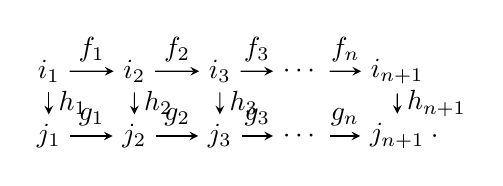
\begin{tikzpicture}[>=stealth,scale=0.53,every node/.style={}]
    \node (i1) at (0,1.55) {$i_1$};
    \node (i2) at (2.05,1.55) {$i_2$};
    \node (i3) at (4.10,1.55) {$i_3$};
    \node (idots) at (6.05,1.55) {$\cdots$};
    \node (in) at (8.35,1.55) {$i_{n+1}$};
    \node (j1) at (0,0) {$j_1$};
    \node (j2) at (2.05,0) {$j_2$};
    \node (j3) at (4.10,0) {$j_3$};
    \node (jdots) at (6.05,0) {$\cdots$};
    \node (jn) at (8.35,0) {$j_{n+1}$};
    \draw[->] (i1) -- node[above] {$f_1$} (i2);
    \draw[->] (i2) -- node[above] {$f_2$} (i3);
    \draw[->] (i3) -- node[above] {$f_3$} (idots);
    \draw[->] (idots) -- node[above] {$f_n$} (in);
    \draw[->] (j1) -- node[above] {$g_1$} (j2);
    \draw[->] (j2) -- node[above] {$g_2$} (j3);
    \draw[->] (j3) -- node[above] {$g_3$} (jdots);
    \draw[->] (jdots) -- node[above] {$g_n$} (jn);
    \draw[->] (i1) -- node[right] {$h_1$} (j1);
    \draw[->] (i2) -- node[right] {$h_2$} (j2);
    \draw[->] (i3) -- node[right] {$h_3$} (j3);
    \draw[->] (in) -- node[right] {$h_{n+1}$} (jn);
    \node at (9.25,0) {$.$};
  \end{tikzpicture}
\end{center}
\VerdierSemanticAnchor{ch1-3-3-6-composition}
射の合成は明らかな仕方で定義される。$\mathrm{Fl}_n(\mathcal{J})$ で
$\mathcal{F}\ell_n(\mathcal{J})$ の対象全体の集合を表す。

\VerdierSemanticAnchor{ch1-3-3-6-cone-functor}
$i\xrightarrow{f}j$ を $\mathcal{F}\ell_1(\mathcal{J})$ の対象とする。関手 $F$ を
適用すると、$\operatorname{comp}(C)$ における射
\[
  F(i)\xrightarrow{F(f)}F(j),
\]
が得られる。これは $\operatorname{Tr}_1(C)$ の対象とみなせるので、写像錐関手を
適用することにより、関手
$S\colon\mathcal{F}\ell_1(\mathcal{J})\longrightarrow\mathrm{K}(C)$ を得る。

\VerdierSemanticAnchor{ch1-3-3-6-1}
\begin{equation}
  S(f)=S\bigl(i\xrightarrow{f}j\bigr)
  =c\bigl(F(i)\xrightarrow{F(f)}F(j)\bigr).
  \tag{3.3.6.1}
\end{equation}
\endgroup

\VerdierSourcePageBlock{0101}%
\begingroup
\VerdierSemanticAnchor{ch1-3-3-6-two-arrow-object}
いま、$i\xrightarrow{f}j\xrightarrow{g}k$ を
$\mathcal{F}\ell_2(\mathcal{J})$ の対象とする。これに
$\operatorname{Tr}_1(C)$ における次の図式を対応させる。

\VerdierSemanticAnchor{ch1-3-3-6-2}
\begin{equation}
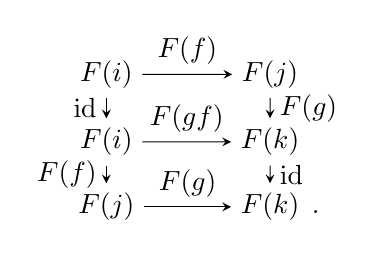
\begin{tikzpicture}[>=stealth,baseline=(current bounding box.center),scale=0.66,
  every node/.style={}]
  \node (Fi1) at (0,2.55) {$F(i)$};
  \node (Fj1) at (3.15,2.55) {$F(j)$};
  \node (Fi2) at (0,1.25) {$F(i)$};
  \node (Fk1) at (3.15,1.25) {$F(k)$};
  \node (Fj2) at (0,0) {$F(j)$};
  \node (Fk2) at (3.15,0) {$F(k)$};
  \draw[->] (Fi1) -- node[above] {$F(f)$} (Fj1);
  \draw[->] (Fi2) -- node[above] {$F(gf)$} (Fk1);
  \draw[->] (Fj2) -- node[above] {$F(g)$} (Fk2);
  \draw[->] (Fi1) -- node[left] {$\mathrm{id}$} (Fi2);
  \draw[->] (Fj1) -- node[right] {$F(g)$} (Fk1);
  \draw[->] (Fi2) -- node[left] {$F(f)$} (Fj2);
  \draw[->] (Fk1) -- node[right] {$\mathrm{id}$} (Fk2);
  \node[anchor=base west,inner sep=0pt,xshift=.08em] at (Fk2.base east) {$.$};
\end{tikzpicture}
\tag{3.3.6.2}
\end{equation}

\VerdierSemanticAnchor{ch1-3-3-6-delta}
次のようにおく。
\begin{equation}
\begin{aligned}
  \delta(f,g)&\colon S(g)\longrightarrow S(f)[1],\\
  \delta(f,g)&=\dot p(F(f))[1]\dot q(F(g)).
\end{aligned}
\tag{3.3.6.3}
\end{equation}
図式 (3.3.6.2) に写像錐関手を適用すると、
$\mathcal{F}\ell_2(\mathcal{J})$ から $K(C)$ における三角の圏への関手を得る。

\VerdierSemanticAnchor{ch1-3-3-6-4}
\begin{equation}
  \bigl(i\xrightarrow{f}j\xrightarrow{g}k\bigr)
  \longmapsto
  S(f)\longrightarrow S(gf)\longrightarrow S(g)
  \xrightarrow{\delta(f,g)}S(f)[1].
  \tag{3.3.6.4}
\end{equation}
\VerdierSemanticAnchor{ch1-3-3-6-distinguished-conclusion}
(3.3.5) の証明の末尾から、三角
\[
  S(f)\longrightarrow S(gf)\longrightarrow S(g)
  \xrightarrow{\delta(f,g)}S(f)[1]
\]
は完全三角であることが分かる。

\VerdierSemanticAnchor{ch1-3-4}
\subsection{完全三角の関手的性質}

\VerdierSemanticAnchor{ch1-3-4-1}
\noindent\textbf{命題 3.4.1.}\quad
$\iota_1\colon K(C)^{\circ}\longrightarrow K(C^{\circ})$ を典型同型
(2.5.13) とし、
\[
  X\xrightarrow{u}Y\xrightarrow{v}Z\xrightarrow{w}X[1]
\]
を $K(C)$ における完全三角とする。このとき、$K(C^{\circ})$ における三角
\VerdierSemanticAnchor{ch1-3-4-1-opposite-triangle}
\[
  (\iota_1X)[-1]\xrightarrow{\iota_1w}\iota_1Z
  \xrightarrow{\iota_1v}\iota_1Y
  \xrightarrow{-\iota_1u}\iota_1X
\]
は完全三角である。
\endgroup

\VerdierSourcePageBlock{0102}%
\begingroup
\VerdierSemanticAnchor{ch1-3-4-1-proof}
(3.3.1) により、与えられた三角が次の形であると常に仮定できる。

\VerdierSemanticAnchor{ch1-3-4-1-cone-model}
\[
  X\xrightarrow{\dot f}Y\xrightarrow{\dot p(f)}c(f)
  \xrightarrow{\dot q(f)}X[1]
\]
ここで $f\colon X\longrightarrow Y$ は $\operatorname{comp}(C)$ における射で
ある。したがって、三角

\VerdierSemanticAnchor{ch1-3-4-1-goal-triangle}
\[
  (\iota_1X)[-1]\xrightarrow{\iota_1\dot q(f)}\iota_1c(f)
  \xrightarrow{\iota_1\dot p(f)}\iota_1Y
  \xrightarrow{-(\iota_1\dot f)}\iota_1X
\]
が完全三角であることを示せばよい（$\iota_1f$ は射 $f$ の
$\iota_1\colon\operatorname{comp}(C)^{\circ}\longrightarrow
\operatorname{comp}(C^{\circ})$ による像である）。$\iota_1$ の定義 (2.4.1) と
写像錐関手の定義 (3.1.2) から、複体 $\iota_1c(f)$ の成分と微分は直ちに
次のようになる。

\VerdierSemanticAnchor{ch1-3-4-1-components}
\[
  \iota_1c(f)^i=(\iota_1X)^{i-1}\oplus(\iota_1Y)^i,
\]
\VerdierSemanticAnchor{ch1-3-4-1-1}
\begin{equation}
  d_{\iota_1c(f)}^i=
  \begin{pmatrix}
    -d_{\iota_1X}^{i-1} & (\iota_1f)^i\\
    0 & d_{\iota_1Y}^{i}
  \end{pmatrix}.
  \tag{3.4.1.1}
\end{equation}
\VerdierSemanticAnchor{ch1-3-4-1-cone-identity}
したがって、
\[
  \iota_1c(f)=c(-\iota_1f)[-1],
\]
であり、次の図式が可換であることが確かめられる。

\VerdierSemanticAnchor{ch1-3-4-1-comparison}
\begin{center}
  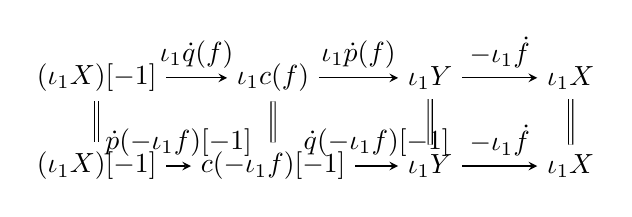
\begin{tikzpicture}[>=stealth,scale=0.70,every node/.style={}]
    \node (x1) at (0,1.60) {$(\iota_1X)[-1]$};
    \node (c1) at (3.20,1.60) {$\iota_1c(f)$};
    \node (y1) at (6.05,1.60) {$\iota_1Y$};
    \node (z1) at (8.60,1.60) {$\iota_1X$};
    \node (x2) at (0,0) {$(\iota_1X)[-1]$};
    \node (c2) at (3.20,0) {$c(-\iota_1f)[-1]$};
    \node (y2) at (6.05,0) {$\iota_1Y$};
    \node (z2) at (8.60,0) {$\iota_1X$};
    \draw[->] (x1) -- node[above] {$\iota_1\dot q(f)$} (c1);
    \draw[->] (c1) -- node[above] {$\iota_1\dot p(f)$} (y1);
    \draw[->] (y1) -- node[above] {$-\iota_1\dot f$} (z1);
    \draw[->] (x2) -- node[above] {$\dot p(-\iota_1f)[-1]$} (c2);
    \draw[->] (c2) -- node[above] {$\dot q(-\iota_1f)[-1]$} (y2);
    \draw[->] (y2) -- node[above] {$-\iota_1\dot f$} (z2);
    \draw[double,double distance=1.1pt] (x1) -- (x2);
    \draw[double,double distance=1.1pt] (c1) -- (c2);
    \draw[double,double distance=1.1pt] (y1) -- (y2);
    \draw[double,double distance=1.1pt] (z1) -- (z2);
  \end{tikzpicture}
\end{center}
\VerdierSemanticAnchor{ch1-3-4-1-proof-complete}
そこで (3.3.3) を適用すれば証明が完了する。

\VerdierSemanticAnchor{ch1-3-4-2}
\noindent\textbf{3.4.2.}\quad
\VerdierSemanticAnchor{ch1-3-4-2-multiadditive-functor}
$F\colon\prod_{i\in[n]}C_i\longrightarrow C$ を多加法的関手とする。
話を具体的にするため、$C$ において可算積が表現可能であると仮定する。
\[
  K_{\Pi}F\colon\prod_{i\in[n]}K(C_i)\longrightarrow K(C)
\]
\VerdierSemanticAnchor{ch1-3-4-2-homotopy-extension}
を $F$ の複体のホモトピー圏への $\Pi$-拡張とし、

\VerdierSemanticAnchor{ch1-3-4-2-shift-isomorphisms}
\[
  p_i\colon K_{\Pi}F(X_1,\ldots,X_i[1],\ldots,X_n)
  \longrightarrow K_{\Pi}F(X_1,\ldots,X_i,\ldots,X_n)[1]
\]
を標準的な関手同型とする。
\endgroup

\VerdierSourcePageBlock{0103}%
\begingroup
\VerdierSemanticAnchor{ch1-3-4-2-variable-specialization}
$j\in[n]$ とし、各 $i\neq j$ に対して $X_i$ を $K(C_i)$ の対象とする。
\[
  G\colon K(C_j)\longrightarrow K(C)
\]
で関手

\VerdierSemanticAnchor{ch1-3-4-2-1}
\begingroup
\makeatletter
\tagsleft@true
\let\veqno\@@leqno
\makeatother
\begin{equation}
  X\longmapsto G(X)=K_{\Pi}F(X_1,\ldots,X,\ldots,X_n),
  \tag{3.4.2.1}
\end{equation}
\endgroup
\VerdierSemanticAnchor{ch1-3-4-2-translation-isomorphism}
を表し、
\[
  m\colon G(X[1])\xrightarrow{\sim}G(X)[1]
\]
で $p_j$ から導かれる関手同型を表す。

\VerdierSemanticAnchor{ch1-3-4-3}
\noindent\textbf{命題 3.4.3.}\quad
\emph{$K(C_j)$ における任意の完全三角}
\VerdierSemanticAnchor{ch1-3-4-3-input-triangle}
\[
  X\xrightarrow{u}Y\xrightarrow{v}Z\xrightarrow{w}X[1]
\]
\emph{に対し、$K(C)$ における三角}
\VerdierSemanticAnchor{ch1-3-4-3-image-triangle}
\[
  G(X)\xrightarrow{G(u)}G(Y)\xrightarrow{G(v)}G(Z)
  \xrightarrow{mG(w)}G(X)[1]
\]
\emph{は完全三角である。}

\VerdierSemanticAnchor{ch1-3-4-3-proof}
まず、$K(C_j)$ における完全三角が (3.3.1) の形
\VerdierSemanticAnchor{ch1-3-4-3-cone-model}
\[
  X\xrightarrow{\dot f}Y\xrightarrow{\dot p(f)}c(f)
  \xrightarrow{\dot q(f)}X[1],
\]
をしていると仮定できる。ここで $f\colon X\longrightarrow Y$ は
$\operatorname{comp}(C_j)$ における射である。
\VerdierSemanticAnchor{ch1-3-4-3-complex-functor}
\[
  H\colon\operatorname{comp}(C_j)\longrightarrow\operatorname{comp}(C)
\]
で関手
\[
  X\longmapsto H(X)=\operatorname{comp}_{\Pi}F
  (X_1,\ldots,X,\ldots,X_n),
\]
\VerdierSemanticAnchor{ch1-3-4-3-complex-translation-isomorphism}
を表し、
\[
  m\colon H(X[1])\xrightarrow{\sim}H(X)[1]
\]
で方向 $j$ のシフトと可換な関手同型を表す。関手 $(G,m)$ は関手 $(H,m)$
を複体のホモトピー圏へ移すことによって得られる。命題を証明するには、
$\operatorname{comp}(C)$ における複体の同型

\VerdierSemanticAnchor{ch1-3-4-3-cone-isomorphism}
\[
  J\colon H(c(f))\xrightarrow{\sim}c(H(f))
\]
で、次の図式を可換にするものが存在することを示せば十分である。

\VerdierSemanticAnchor{ch1-3-4-3-1}
\begin{equation}
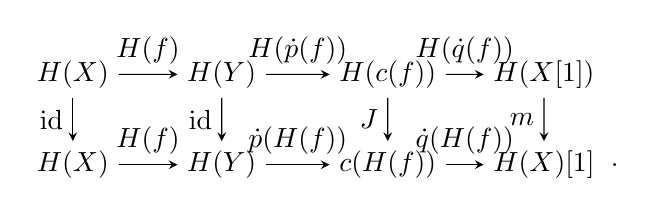
\begin{tikzpicture}[>=stealth,scale=0.62,every node/.style={}]
  \node (x1) at (0,1.85) {$H(X)$};
  \node (y1) at (3.05,1.85) {$H(Y)$};
  \node (c1) at (6.45,1.85) {$H(c(f))$};
  \node (s1) at (9.65,1.85) {$H(X[1])$};
  \node (x2) at (0,0) {$H(X)$};
  \node (y2) at (3.05,0) {$H(Y)$};
  \node (c2) at (6.45,0) {$c(H(f))$};
  \node (s2) at (9.65,0) {$H(X)[1]$};
  \draw[->] (x1) -- node[above] {$H(f)$} (y1);
  \draw[->] (y1) -- node[above] {$H(\dot p(f))$} (c1);
  \draw[->] (c1) -- node[above] {$H(\dot q(f))$} (s1);
  \draw[->] (x2) -- node[above] {$H(f)$} (y2);
  \draw[->] (y2) -- node[above] {$\dot p(H(f))$} (c2);
  \draw[->] (c2) -- node[above] {$\dot q(H(f))$} (s2);
  \draw[->] (x1) -- node[left] {$\mathrm{id}$} (x2);
  \draw[->] (y1) -- node[left] {$\mathrm{id}$} (y2);
  \draw[->] (c1) -- node[left] {$J$} (c2);
  \draw[->] (s1) -- node[left] {$m$} (s2);
  \node[anchor=west,inner sep=0pt] at ([xshift=0.35em]s2.east) {$.$};
\end{tikzpicture}
\tag{3.4.3.1}
\end{equation}
\endgroup

\VerdierSourcePageBlock{0104}%
\begingroup
\VerdierSemanticAnchor{ch1-3-4-3-zero-differential-complex}
各複体 $X$ に対し、$X$ の成分を保ち、微分を零とした複体を
$\overline{X}$ で表す。$H$ の定義から直ちに
$\overline{H(X)}=H(\overline{X})$ を得る。同様に、各複体の射
$f\colon X\longrightarrow Y$ に対し、$f$ の成分を保って得られる射を
$\overline{f}\colon\overline{X}\longrightarrow\overline{Y}$ で表す。写像錐関手の
定義から、$c(\overline{f})=\overline{Y}\oplus\overline{X[1]}$ であり、
$p(\overline{f})\colon\overline{Y}\longrightarrow c(\overline{f})$ は第一成分への
標準的包含射、
$q(\overline{f})\colon c(\overline{f})\longrightarrow\overline{X[1]}$ は第二成分への
標準的射影である。

\VerdierSemanticAnchor{ch1-3-4-3-cone-graded-splitting}
関手 $H$ と関手「$\overline{\phantom{X}}$」は加法的なので、
$\overline{H(c(f))}=\overline{H(Y)}\oplus\overline{H(X[1])}$ となり、
$\overline{H(p(f))}\colon\overline{H(Y)}\longrightarrow\overline{H(c(f))}$ は第一
成分への標準的包含射、
$\overline{H(q(f))}\colon\overline{H(c(f))}\longrightarrow\overline{H(X[1])}$ は
第二成分への標準的射影となる。したがって、
\[
  H(c(f))^l=H(Y)^l\oplus H(X[1])^l,
\]

\VerdierSemanticAnchor{ch1-3-4-3-2}
\begin{equation}
  d_{H(c(f))}^{,l}=
  \begin{pmatrix}
    d_{H(Y)}^{,l} & \Phi^l\\
    0 & d_{H(X[1])}^{,l}
  \end{pmatrix},
  \tag{3.4.3.2}
\end{equation}

\VerdierSemanticAnchor{ch1-3-4-3-phi-map}
\[
  \Phi^l\colon H(X[1])^l\longrightarrow H(Y)^{l+1}.
\]
$H(c(f))$ の微分がこの形になるのは、単に $H(p(f))$ と $H(q(f))$ が複体の
射であることを表したからである。$\Phi^l$ を計算するには、関手 $H$ の定義、
したがって付随する単純複体の関手の定義 (2.2.2.5) に戻る必要がある。次を得る。

\VerdierSemanticAnchor{ch1-3-4-3-x-shift-components}
\[
  H(X[1])^l=
  \prod_{\substack{\sigma=\sum_i l_i e_i\\ \sum_i l_i=l}}
  F(X_1^{l_1},\ldots,X^{l_j+1},\ldots,X_n^{l_n}),
\]

\VerdierSemanticAnchor{ch1-3-4-3-3}
\begin{equation}
  H(Y)^{l+1}=
  \prod_{\substack{\sigma=\sum_i l_i e_i\\ \sum_i l_i=l}}
  F(X_1^{l_1},\ldots,Y^{l_j+1},\ldots,X_n^{l_n}),
  \tag{3.4.3.3}
\end{equation}

\VerdierSemanticAnchor{ch1-3-4-3-phi-components}
\[
  \Phi^l=
  \prod_{\substack{\sigma=\sum_i l_i e_i\\ \sum_i l_i=l}}
  \varepsilon(\sigma,j)
  F(X_1^{l_1},\ldots,f^{l_j+1},\ldots,X_n^{l_n}).
\]
\endgroup

\VerdierSourcePageBlock{0105}%
\begingroup
\VerdierSemanticAnchor{ch1-3-4-3-cone-of-hf}
一方、写像錐関手の定義から次を得る。
\[
  c(H(f))^l=H(Y)^l\oplus(H(X)[1])^l,
\]

\VerdierSemanticAnchor{ch1-3-4-3-4}
\begin{equation}
  d_{c(H(f))}^{,l}=
  \begin{pmatrix}
    d_{H(Y)}^{,l} & H(f)^{l+1}\\
    0 & d_{H(X)[1]}^{,l}
  \end{pmatrix},
  \tag{3.4.3.4}
\end{equation}
ここで射 $H(f)$ は (2.4.2.6)、(2.4.2.3)、(2.2.2.6) により定義される。

\VerdierSemanticAnchor{ch1-3-4-3-5}
\begin{equation}
  H(f)^{l+1}=
  \prod_{\substack{\sigma=\sum_i l_i e_i\\ \sum_i l_i=l}}
  F(X_1^{l_1},\ldots,f^{l_j+1},\ldots,X_n^{l_n}).
  \tag{3.4.3.5}
\end{equation}

\VerdierSemanticAnchor{ch1-3-4-3-j-map}
ここで次のようにおく。
\[
  J^l\colon H(Y)^l\oplus H(X[1])^l
  \longrightarrow H(Y)^l\oplus(H(X)[1])^l,
\]

\VerdierSemanticAnchor{ch1-3-4-3-6}
\begin{equation}
  J^l=
  \begin{pmatrix}
    \operatorname{id}_{H(Y)^l} & 0\\
    0 & \Psi^l
  \end{pmatrix},
  \qquad
  \Psi^l=
  \prod_{\substack{\sigma=\sum_i l_i e_i\\ \sum_i l_i=l}}
  \varepsilon(\sigma,j)
  \operatorname{id}_{F(X_1^{l_1},\ldots,X^{l_j+1},\ldots,X_n^{l_n})}.
  \tag{3.4.3.6}
\end{equation}

\VerdierSemanticAnchor{ch1-3-4-3-7}
各 $J^l$ が複体の射の成分であることを確かめるには、次を確かめれば十分で
ある。
\begin{equation}
  \Phi^l=H(f)^{l+1}\Psi^l,
  \qquad
  \Psi^{l+1}d_{H(X[1])}^{l}=d_{H(X)[1]}^{l}\Psi^l.
  \tag{3.4.3.7}
\end{equation}

\VerdierSemanticAnchor{ch1-3-4-3-8}
図式 (3.4.3.1) が可換であることを確かめるには、次を確かめれば十分である。
\begin{equation}
  \Psi^l=m^l.
  \tag{3.4.3.8}
\end{equation}
\endgroup

\VerdierSourcePageBlock{0106}%
\begingroup


\VerdierSemanticAnchor{ch1-3-4-3-verification}
(3.4.3.7) の第一の等式は明らかである（(3.4.3.3) と (3.4.3.5)）。
(3.4.3.7) の第二の等式は (3.4.3.8) から従う。(3.4.3.8) を確かめるには、
射 $m$ の定義 (2.3.2.1) を参照すれば十分である。

\VerdierSemanticAnchor{ch1-3-4-4}
\noindent\textbf{3.4.4.}\quad
$C$ において可算直和が表現可能であるとき、関手 $K_{\Sigma}F$ について命題
(3.4.3) と同様の命題が成り立つ。その証明は、命題 (3.4.3) の証明において
積を直和で置き換えることによって得られる。
\endgroup

\VerdierSourcePageSilent{0107}%

\clearpage
\VerdierSourcePageBlock{0108}%
\begingroup
\VerdierSemanticAnchor{ch1-app-signs}
\section*{付録：符号の選択に関する注記}
\addcontentsline{toc}{section}{付録：符号の選択に関する注記}

\VerdierSemanticAnchor{ch1-app-signs-cone}
写像錐関手は、その随伴性 (3.1.3) により一意な同型を除いて定まる。
$\operatorname{tr}_1(C)$ の射に $\operatorname{comp}(C)$ の三角を容易に対応させる
ため、シフト関手として「射 $X\longrightarrow 0$ の写像錐」を選んだ
（(3.1.7) および (3.2.2.7)）。すなわち、次数をずらし、微分の符号を変える。

\VerdierSemanticAnchor{ch1-app-signs-strict}
$F\colon\prod_{i\in[n]}C_i\longrightarrow C$ を多加法的関手とする。圏
$\prod_{i\in[n]}\operatorname{comp}(C_i)$ は自然に $\mathbb Z[n]$-圏の構造をもつ。
関手
\[
  F^{[n]}\colon\prod_{i\in[n]}\operatorname{comp}(C_i)
  \longrightarrow\operatorname{comp}^{n}(C)
\]
を厳密な $\mathbb Z[n]$-関手にしようとすると、われわれが採用したシフトの
規約、すなわち一つの方向に次数をずらし、対応する微分の符号を変えるという
選択に導かれる。

\VerdierSemanticAnchor{ch1-app-signs-simple-complex}
付随する単純複体関手の選択には [1] の規約を採用した（ただし、われわれの
多重複体では微分どうしは可換である）。これにより関手
$K_{\Pi}F\colon\prod_i K(C_i)\longrightarrow K(C)$ を定義できる。このとき
$K_{\Pi}F(X_1,\ldots,X_i[1],\ldots,X_n)$ は
$K_{\Pi}F(X_1,\ldots,X_i,\ldots,X_n)[1]$ と異なる。それでも関手
$K_{\Pi}F$ が完全三角を完全三角に送ると述べるために、同型

\VerdierSemanticAnchor{ch1-app-signs-shift-isomorphism}
\[
  p_i\colon K_{\Pi}F(X_1,\ldots,X_i[1],\ldots,X_n)
  \xrightarrow{\ \sim\ }
  K_{\Pi}F(X_1,\ldots,X_i,\ldots,X_n)[1]
\]
を定義することになる（(3.4.3) の証明）。

\VerdierSemanticAnchor{ch1-app-signs-anticommutativity}
すると $i\ne j$ のとき、次の反可換図式が得られる。

\VerdierSemanticAnchor{ch1-app-signs-diagram}
\begin{center}
  \mbox{%
    $\begin{tikzcd}[ampersand replacement=\&,column sep=3.2em,row sep=4.3em]
      K_{\Pi}F(X_1,\ldots,X_i[1],\ldots,X_j[1],\ldots)
        \arrow[r,"p_j"]
        \arrow[d,"p_i"']
        \& K_{\Pi}F(X_1,\ldots,X_i[1],\ldots,X_j,\ldots)[1]
          \arrow[d,"p_i"] \\
      K_{\Pi}F(X_1,\ldots,X_i,\ldots,X_j[1],\ldots)[1]
        \arrow[r,"p_j"]
        \& K_{\Pi}F(X_1,\ldots,X_i,\ldots,X_j,\ldots)[2].
    \end{tikzcd}$%
  }
\end{center}

\VerdierSemanticAnchor{ch1-app-signs-koszul-choice}
続いて (1.5.2) では、これらの同型を同型 $p(\sigma)$ へ整合的に拡張する
方法を示した。この同型は各 $\sigma\in\mathbb Z[n]$ に対して定義される。
ここには一つの
任意な選択が入る。それは、それ自身はよく定まったコホモロジー類、すなわち
Koszul 類 (1.6.3) の中で余サイクルを選ぶことである。一般に受け入れられている
規則（例えば [1]）に合わせるため、すべての場合に Koszul 余サイクル (1.6.6)
を選んだ。
\endgroup

\VerdierSourcePageSilent{0109}%

\clearpage
\chapter{三角圏}
\VerdierSourcePageBlock{0110}%
\VerdierSemanticAnchor{ch2}
\begingroup
\VerdierSemanticAnchor{ch2-1}
\section{定義と初歩的性質}

\VerdierSemanticAnchor{ch2-1-1}
\subsection{三角圏の定義}

\VerdierSemanticAnchor{ch2-1-1-1}
\noindent\textbf{定義 1.1.1.}\quad
\emph{三角圏} $\mathcal D$ とは、三角（第 I 章、3.2.1）の族を備えた厳密な
加法的 $\mathbb Z$-圏（第 I 章、1.5.11）であって、それらの三角を
\emph{完全三角}と呼び、次の性質を満たすものをいう。

\VerdierSemanticAnchor{ch2-1-1-1-tri}
\smallskip
\noindent\textbf{TRI:}
$\mathcal D$ の三角で完全三角に同型なものは、すべて完全三角である。任意の
対象 $X$（$\mathcal D$ の対象）に対し、三角
\[
  X\xrightarrow{\operatorname{id}_X}X\longrightarrow 0
  \longrightarrow X[1]
\]
は完全三角である。任意の射 $u\colon X\longrightarrow Y$（$\mathcal D$ の射）は、
次の完全三角に含まれる。
\[
  X\xrightarrow{u}Y\xrightarrow{v}Z\xrightarrow{w}X[1].
\]

\VerdierSemanticAnchor{ch2-1-1-1-trii}
\noindent\textbf{TRII:}
$\mathcal D$ の三角
\[
  X\xrightarrow{u}Y\xrightarrow{v}Z\xrightarrow{w}X[1]
\]
が完全三角であるための必要十分条件は、三角
\[
  Y\xrightarrow{v}Z\xrightarrow{w}X[1]
  \xrightarrow{-u[1]}Y[1]
\]
が完全三角であることである。

\VerdierSemanticAnchor{ch2-1-1-1-triii}
\noindent\textbf{TRIII:}
任意の二つの完全三角

\VerdierSemanticAnchor{ch2-1-1-1-triii-triangles}
\[
  \begin{aligned}
    X  &\xrightarrow{u}  Y  \xrightarrow{v}  Z  \xrightarrow{w}  X[1],\\
    X' &\xrightarrow{u'} Y' \xrightarrow{v'} Z' \xrightarrow{w'} X'[1]
  \end{aligned}
\]
と任意の可換図式

\VerdierSemanticAnchor{ch2-1-1-1-triii-square}
\begin{center}
  \begin{tikzcd}[column sep=4.5em,row sep=3em]
    X \arrow[r,"u"] \arrow[d,"f"'] & Y \arrow[d,"g"] \\
    X' \arrow[r,"u'"] & Y'\,,
  \end{tikzcd}
\end{center}
\endgroup%
\VerdierSourcePageContinue{0111}%
\begingroup
\VerdierSemanticAnchor{ch2-1-1-1-triii-filler}
\noindent 射 $h\colon Z\longrightarrow Z'$ であって、$(f,g,h)$ が三角の射と
なるものが存在する。すなわち、次の図式は可換である。

\VerdierSemanticAnchor{ch2-1-1-1-triii-morphism-diagram}
\begin{center}
  \begin{tikzcd}[column sep=3.6em,row sep=2.8em]
    X \arrow[r,"u"] \arrow[d,"f"']
      & Y \arrow[r,"v"] \arrow[d,"g"']
      & Z \arrow[r,"w"] \arrow[d,"h"']
      & X[1] \arrow[d,"{f[1]}"] \\
    X' \arrow[r,"u'"]
      & Y' \arrow[r,"v'"]
      & Z' \arrow[r,"w'"]
      & X'[1] .
\end{tikzcd}
\end{center}

\VerdierSemanticAnchor{ch2-1-1-1-triv}
\noindent\textbf{TRIV:}
任意の可換図式

\VerdierSemanticAnchor{ch2-1-1-1-triv-input}
\begin{center}
  \begin{tikzcd}[column sep=4.3em,row sep=2.7em]
    & X_2 \arrow[dr,"u_1"] & \\
    X_1 \arrow[ur,"u_3"] \arrow[rr,"u_2"] && X_3
  \end{tikzcd}
\end{center}
と任意の三つの完全三角

\VerdierSemanticAnchor{ch2-1-1-1-triv-triangles}
\[
  \begin{aligned}
    X_1 &\xrightarrow{u_3} X_2 \xrightarrow{v_3} Z_3
        \xrightarrow{w_3} X_1[1],\\
    X_2 &\xrightarrow{u_1} X_3 \xrightarrow{v_1} Z_1
        \xrightarrow{w_1} X_2[1],\\
    X_1 &\xrightarrow{u_2} X_3 \xrightarrow{v_2} Z_2
        \xrightarrow{w_2} X_1[1],
  \end{aligned}
\]

\VerdierSemanticAnchor{ch2-1-1-1-triv-fillers}
に対して、二つの射
\[
  \begin{aligned}
    m_1 &\colon Z_3\longrightarrow Z_2,\\
    m_3 &\colon Z_2\longrightarrow Z_1,
  \end{aligned}
\]

\VerdierSemanticAnchor{ch2-1-1-1-triv-morphisms}
であって、$(\operatorname{id}_{X_1},u_1,m_1)$ と
$(u_3,\operatorname{id}_{X_3},m_3)$ が三角の射となり、さらに三角

\VerdierSemanticAnchor{ch2-1-1-1-triv-distinguished-triangle}
\[
  Z_3\xrightarrow{m_1}Z_2\xrightarrow{m_3}Z_1
  \xrightarrow{v_3[1]w_1}Z_3[1]
\]
が完全三角となるものが存在する。

\VerdierSemanticAnchor{ch2-1-1-2}
\medskip
\noindent\textbf{注意 1.1.2.}\quad
$(X,Y,Z,u,v,w)$ を完全三角とする。TRII から、非有界列

\VerdierSemanticAnchor{ch2-1-1-2-translation-sequence}
\[
  \cdots\longrightarrow X[n]
  \xrightarrow{(-1)^n u[n]}Y[n]
  \xrightarrow{(-1)^n v[n]}Z[n]
  \xrightarrow{(-1)^n w[n]}X[n+1]
  \longrightarrow\cdots
\]
において、連続する三つの射が完全三角をなすことが分かる。

\VerdierSemanticAnchor{ch2-1-1-2-translation-automorphisms}
$\mathcal D\colon X\longmapsto X[n]$ の自己同型を\emph{シフト自己同型}と呼ぶ。
\endgroup

\VerdierSourcePageBlock{0112}%
\begingroup
\VerdierSemanticAnchor{ch2-1-1-3}
\noindent\textbf{定義 1.1.3.}\quad
$\mathcal D$ と $\mathcal D'$ を二つの三角圏とする。$\mathcal D$ から
$\mathcal D'$ への\emph{完全関手}とは、（必ずしも厳密ではない）
$\mathbb Z$-関手（第 I 章、1.2.4）
$(F,p)\colon\mathcal D\longrightarrow\mathcal D'$ であって、
$\mathcal D$ の任意の完全三角

\VerdierSemanticAnchor{ch2-1-1-3-source-triangle}
\[
  X\xrightarrow{u}Y\xrightarrow{v}Z\xrightarrow{w}X[1]
\]
に対し、三角

\VerdierSemanticAnchor{ch2-1-1-3-image-triangle}
\[
  FX\xrightarrow{Fu}FY\xrightarrow{Fv}FZ
  \xrightarrow{p(X)Fw}(FX)[1]
\]
が完全三角となるものをいう (1.1.4.2)。

\VerdierSemanticAnchor{ch2-1-1-4}
\medskip
\noindent\textbf{定義 1.1.4.}\quad
$\mathcal D_i$（$1\leq i\leq n$）および $\mathcal D$ を合わせて
$n+1$ 個の三角圏とする。$\prod_i\mathcal D_i$ から $\mathcal D$ への
\emph{多重完全関手}とは、捩れた $\mathbb Z^n$-関手（第 I 章、1.4.4）
$(F,p)\colon\prod_i\mathcal D_i\longrightarrow\mathcal D$ であって、
それぞれ圏 $\mathcal D_i$ に属する任意の対象族 $X_i$（$i\ne j$）に対し、
$\mathbb Z$-関手

\VerdierSemanticAnchor{ch2-1-1-4-partial-functor}
\[
  X\longmapsto F(X_1,\ldots,X,\ldots,X_n)\colon
  \mathcal D_j\longrightarrow\mathcal D
\]
が完全関手となるものをいう。

\VerdierSemanticAnchor{ch2-1-1-4-1}
\medskip
\noindent\textbf{1.1.4.1.}\quad
定義 (1.1.4) では、圏 $\prod_i\mathcal D_i$ にその標準的な
$\mathbb Z^n$-構造を入れ、群 $\mathbb Z^n$ は準同型

\VerdierSemanticAnchor{ch2-1-1-4-1-group-action}
\[
  \mathbb Z^n\longrightarrow\mathbb Z,
\]
すなわち座標の和を通じて圏 $\mathcal D$ に作用する（第 I 章、1.6.6）。

\VerdierSemanticAnchor{ch2-1-1-4-2}
\medskip
\noindent\textbf{1.1.4.2.}\quad
符号規則 I（第 I 章、1.6.6）に従い、特に断らない限り、多重完全関手は
$\mathbb Z^n$ の標準基底 $e_1,\ldots,e_n$ に関する Koszul 余サイクルで
捩るものとする（第 I 章、1.6.4）。

\VerdierSemanticAnchor{ch2-1-1-4-2-trivial-cocycle}
とりわけ、これは $\mathcal D$ から $\mathcal D'$ への完全関手が自明な
余サイクルで捩られることを意味する。

\VerdierSemanticAnchor{ch2-1-1-5}
\medskip
\noindent\textbf{定義 1.1.5.}\quad
$\mathcal D$ を三角圏、$\mathcal A$ をアーベル圏とする。関手
$H\colon\mathcal D\longrightarrow\mathcal A$ が\emph{コホモロジー的関手}
であるとは、任意の完全三角

\VerdierSemanticAnchor{ch2-1-1-5-source-triangle}
\[
  X\xrightarrow{u}Y\xrightarrow{v}Z\xrightarrow{w}X[1],
\]
に対し、図式

\VerdierSemanticAnchor{ch2-1-1-5-image-sequence}
\[
  HX\xrightarrow{Hu}HY\xrightarrow{Hv}HZ\xrightarrow{Hw}H(X[1])
\]
が $\mathcal A$ の完全列となることをいう。
\endgroup

\VerdierSourcePageBlock{0113}%
\begingroup
\VerdierSemanticAnchor{ch2-1-1-5-additivity-announcement}
\noindent (1.2.7) において、コホモロジー的関手が加法的であり、多重完全関手が
多重加法的であることを示す。

\VerdierSemanticAnchor{ch2-1-1-5-cohomology-notation}
$H\colon\mathcal D\longrightarrow\mathcal A$ をコホモロジー的関手とする。
通常、$H^0(X)=H(X)$、$H^n(X)=H(X[n])$ と書く。公理 TRII を用いると、
コホモロジー的関手は任意の完全三角

\VerdierSemanticAnchor{ch2-1-1-5-long-exact-setup}
\[
  X\xrightarrow{u}Y\xrightarrow{v}Z\xrightarrow{w}X[1]
\]
に長完全列

\VerdierSemanticAnchor{ch2-1-1-5-1}
\begin{equation}
  \cdots\longrightarrow H^{-1}(Z)
  \xrightarrow{H^{-1}(-w)}H^0(X)
  \xrightarrow{H^0(u)}H^0(Y)
  \xrightarrow{H^0(v)}H^0(Z)
  \xrightarrow{H^0(w)}\cdots
  \tag{1.1.5.1}
\end{equation}
を対応させることが分かる。

\VerdierSemanticAnchor{ch2-1-1-6}
\medskip
\noindent\textbf{1.1.6.}\quad
$\mathcal D$ を三角圏とする。通常、次の用語を用いる。$\mathcal D$ の三角

\VerdierSemanticAnchor{ch2-1-1-6-antidistinguished-triangle}
\[
  X\xrightarrow{u}Y\xrightarrow{v}Z\xrightarrow{w}X[1]
\]
が\emph{反完全}であるとは、三角
\[
  X\xrightarrow{u}Y\xrightarrow{v}Z\xrightarrow{-w}X[1]
\]
が完全三角であることをいう。

\VerdierSemanticAnchor{ch2-1-1-6-antiexact-functor}
三角圏 $\mathcal D'$ から $\mathcal D$ への $\mathbb Z$-関手が
\emph{反完全}であるとは、それが $\mathcal D'$ の完全三角を
$\mathcal D$ の反完全三角へ送ることをいう。

\VerdierSemanticAnchor{ch2-1-1-6-exact-functor-notation}
通常、$\mathcal D'$ から $\mathcal D$ への完全関手を記す際には、シフトと
可換する同型を記号から省略する。

\VerdierSemanticAnchor{ch2-1-1-7}
\medskip
\noindent\textbf{1.1.7.}\quad
$\mathcal C$ を厳密な $\mathbb Z$-圏（第 I 章、1.2.2）とし、

\VerdierSemanticAnchor{ch2-1-1-7-translations}
\[
  X\longmapsto X[n],\qquad n\in\mathbb Z,
\]
を $\mathcal C$ のシフト関手とする。$\mathcal C^\circ$ を反対
$\mathbb Z$-圏（第 I 章、1.3.9）とする。

\VerdierSemanticAnchor{ch2-1-1-7-opposite-morphism}
$\mathcal C$ の任意の射 $u$ に対し、$\mathcal C^\circ$ の対応する射を
$((u))$ と書く。$\mathcal C^\circ$ の対象の集合と射の集合は、それぞれ
$\mathcal C$ の対象の集合と射の集合に等しいので、この記法は厳密には
濫用である。$\mathcal C^\circ$ のシフト関手を

\VerdierSemanticAnchor{ch2-1-1-7-opposite-translations}
\[
  X\longmapsto X[[n]],\qquad n\in\mathbb Z,
\]
と書く。

\VerdierSemanticAnchor{ch2-1-1-7-translation-identity}
$\mathcal C$ の任意の対象 $X$ と任意の整数 $n\in\mathbb Z$ に対し
（第 I 章、1.3.9）、
\[
  X[-n]=X[[n]]
\]
であったことを思い出そう。

\VerdierSemanticAnchor{ch2-1-1-7-opposite-category}
三角圏 $\mathcal D$ の\emph{反対三角圏}とは、圏 $\mathcal D$ の厳密な
反対 $\mathbb Z$-圏 $\mathcal D^\circ$（第 I 章、1.3.9）に、次の完全三角の
族を入れたものと定義する。$\mathcal D^\circ$ の三角

\VerdierSemanticAnchor{ch2-1-1-7-opposite-triangle}
\[
  X[[-1]]\xrightarrow{((w))}Z\xrightarrow{((v))}Y
  \xrightarrow{((u))}X
\]
が完全三角であるための必要十分条件は、圏 $\mathcal D$ の対応する三角

\VerdierSemanticAnchor{ch2-1-1-7-corresponding-antitriangle}
\[
  X\xrightarrow{u}Y\xrightarrow{v}Z\xrightarrow{w}X[1]
\]
が反完全三角であることである。

\VerdierSemanticAnchor{ch2-1-1-7-triangulated-axioms}
このように定めた $\mathcal D^\circ$ の三角の族が三角圏の公理を満たすことは、
容易に示される。
\endgroup

\VerdierSourcePageBlock{0114}%
\begingroup
\VerdierSemanticAnchor{ch2-1-2}
\medskip
\noindent\textbf{1.2. 三角圏の初歩的性質。}

\VerdierSemanticAnchor{ch2-1-2-1}
\medskip
\noindent\textbf{命題 1.2.1.}\quad
$\mathcal D$ を三角圏とする。$\mathcal D$ の任意の対象 $X$ に対し、関手
$\operatorname{Hom}_{\mathcal D}(X,\mathord\cdot)$ および
$\operatorname{Hom}_{\mathcal D}(\mathord\cdot,X)$ は、アーベル群の圏に
値をとるコホモロジー的関手である。

\VerdierSemanticAnchor{ch2-1-2-1-hom-functors}
\noindent\emph{証明。}\quad
まず関手 $\operatorname{Hom}_{\mathcal D}(X,\mathord\cdot)$ が
コホモロジー的関手であることを示せば十分である。他方の主張は、反対圏
$\mathcal D^\circ$ (1.1.7) に移ることで従う。そこで

\VerdierSemanticAnchor{ch2-1-2-1-source-triangle}
\[
  X'\xrightarrow{u'}Y'\xrightarrow{v'}Z'\xrightarrow{w'}X'[1]
\]
を完全三角とする。図式

\VerdierSemanticAnchor{ch2-1-2-1-1}
\begin{equation}
  \mbox{$
    \operatorname{Hom}_{\mathcal D}(X,X')
    \xrightarrow{\operatorname{Hom}_{\mathcal D}(X,u')}
    \operatorname{Hom}_{\mathcal D}(X,Y')
    \xrightarrow{\operatorname{Hom}_{\mathcal D}(X,v')}
    \operatorname{Hom}_{\mathcal D}(X,Z')
    \xrightarrow{\operatorname{Hom}_{\mathcal D}(X,w')}
    \operatorname{Hom}_{\mathcal D}(X,X'[1])
  $}
  \tag{1.2.1.1}
\end{equation}

\VerdierSemanticAnchor{ch2-1-2-1-exactness-reduction}
において
\[
  \operatorname{Hom}_{\mathcal D}(X,v')
  \operatorname{Hom}_{\mathcal D}(X,u')=0
\]
であり、かつこの図式が $\operatorname{Hom}_{\mathcal D}(X,Y')$ で完全で
あることを示せばよい。そうすれば公理 TRII により、
$\operatorname{Hom}_{\mathcal D}(X,Z')$ でも同じ結果が得られる。
$f\colon X\longrightarrow X'$ とする。TRI により三角

\VerdierSemanticAnchor{ch2-1-2-1-identity-triangle}
\[
  X\xrightarrow{\operatorname{id}_X}X\longrightarrow0\longrightarrow X[1]
\]
は完全三角であり、TRII と TRIII により、次の図式を可換にする射
$g\colon X\longrightarrow Y'$ が存在する。

\VerdierSemanticAnchor{ch2-1-2-1-2}
\begin{equation}
  \begin{tikzcd}[column sep=3.2em,row sep=2.5em]
    X \arrow[r,"{\operatorname{id}_X}"] \arrow[d,"f"']
      & X \arrow[r] \arrow[d,"g"']
      & 0 \arrow[r] \arrow[d]
      & X[1] \arrow[d,"{f[1]}"] \\
    X' \arrow[r,"u'"']
      & Y' \arrow[r,"v'"']
      & Z' \arrow[r,"w'"']
      & X'[1]
  \end{tikzcd}
  \tag{1.2.1.2}
\end{equation}

\VerdierSemanticAnchor{ch2-1-2-1-zero-composite}
したがって $u'f=g$ かつ $v'u'f=v'g=0$ であり、
$\operatorname{Hom}_{\mathcal D}(X,v')
\operatorname{Hom}_{\mathcal D}(X,u')=0$ が示された。

\VerdierSemanticAnchor{ch2-1-2-1-lifting}
次に $v'g=0$ を満たす射 $g\colon X\longrightarrow Y'$ をとる。TRII と
TRIII により、図式 (1.2.1.2) を可換にする射
$f\colon X\longrightarrow X'$ が存在する。ゆえに $g=u'f$ であり、列
(1.2.1.1) は $\operatorname{Hom}_{\mathcal D}(X,Y')$ で完全である。

\VerdierSemanticAnchor{ch2-1-2-2}
\medskip
\noindent\textbf{系 1.2.2.}\quad
完全三角
$X'\xrightarrow{u'}Y'\xrightarrow{v'}Z'\xrightarrow{w'}X'[1]$ では、
連続する任意の二射の合成は零である。

\VerdierSemanticAnchor{ch2-1-2-2-proof}
\noindent\emph{証明。}\quad
TRII により $v'u'=0$ を示せば十分である。そのためには、完全列
(1.2.1.1) で $X=X'$ とし、
$\operatorname{id}_{X'}\in\operatorname{Hom}_{\mathcal D}(X',X')$ の
連続する像を考えればよい。

\VerdierSemanticAnchor{ch2-1-2-3}
\medskip
\noindent\textbf{系 1.2.3.}\quad
$(X,Y,Z,u,v,w)$ と $(X',Y',Z',u',v',w')$ を $\mathcal D$ の二つの
完全三角とし、$(f_1,f_2,f_3)$ を三角の射とする。三つの $f_i$
（$1\leq i\leq3$）のうち二つが同型ならば、残りの一つも同型である。
\endgroup

\VerdierSourcePageBlock{0115}%
\begingroup
\VerdierSemanticAnchor{ch2-1-2-3-proof-f1-f2}
具体的に、$f_1\colon X\longrightarrow X'$ と
$f_2\colon Y\longrightarrow Y'$ が同型である場合を考える。$\mathcal D$ の
任意の対象 $W$ に対し、次の可換図式がある。

\VerdierSemanticAnchor{ch2-1-2-3-five-lemma-diagram}
\begin{equation*}
  \mbox{%
    $\begin{tikzcd}[ampersand replacement=\&,column sep=2.15em,row sep=3em]
      \cdots \arrow[r]
        \& \operatorname{Hom}_{\mathcal D}(W,X) \arrow[r] \arrow[d,"{\operatorname{Hom}_{\mathcal D}(W,f_1)}"']
        \& \operatorname{Hom}_{\mathcal D}(W,Y) \arrow[r] \arrow[d,"{\operatorname{Hom}_{\mathcal D}(W,f_2)}"']
        \& \operatorname{Hom}_{\mathcal D}(W,Z) \arrow[r] \arrow[d,"{\operatorname{Hom}_{\mathcal D}(W,f_3)}"']
        \& \operatorname{Hom}_{\mathcal D}(W,X[1]) \arrow[r] \arrow[d,"{\operatorname{Hom}_{\mathcal D}(W,f_1[1])}"']
        \& \cdots \\
      \cdots \arrow[r]
        \& \operatorname{Hom}_{\mathcal D}(W,X') \arrow[r]
        \& \operatorname{Hom}_{\mathcal D}(W,Y') \arrow[r]
        \& \operatorname{Hom}_{\mathcal D}(W,Z') \arrow[r]
        \& \operatorname{Hom}_{\mathcal D}(W,X'[1]) \arrow[r]
        \& \cdots
    \end{tikzcd}$%
  }\,.
\end{equation*}

\VerdierSemanticAnchor{ch2-1-2-3-five-lemma}
各行は完全である。五項補題により、
$\operatorname{Hom}_{\mathcal D}(W,f_3)$ は任意の $W$ に対して同型であり、
したがって $f_3$ も同型である。系の残る二つの主張は、公理 TRII を用いて
この場合から従う。

\VerdierSemanticAnchor{ch2-1-2-4}
\medskip
\noindent\textbf{系 1.2.4.}\quad
$X\xrightarrow{u}Y\xrightarrow{v}Z\xrightarrow{w}X[1]$ と
$X\xrightarrow{u}Y\xrightarrow{v'}Z'\xrightarrow{w'}X[1]$ を二つの
完全三角とする。このとき、次の図式を可換にする同型
$f\colon Z\xrightarrow{\sim}Z'$ が存在する。

\VerdierSemanticAnchor{ch2-1-2-4-1}
\begin{equation}
  \begin{tikzcd}[column sep=2.8em,row sep=1.7em]
    && Z \arrow[dr,"w"] \arrow[dd,"f"',"\sim"] & \\
    X \arrow[r,"u"] & Y \arrow[ur,"v"] \arrow[dr,"v'"'] && X[1] \\
    && Z' \arrow[ur,"w'"'] &
  \end{tikzcd}
  \tag{1.2.4.1}
\end{equation}

\VerdierSemanticAnchor{ch2-1-2-4-proof}
実際、公理 TRIII により、図式 (1.2.4.1) を可換にする射
$f\colon Z\longrightarrow Z'$ が存在する。(1.2.3) により、この射は同型で
ある。

\VerdierSemanticAnchor{ch2-1-2-4-essential-uniqueness}
したがって系 (1.2.4) は、与えられた射を含む完全三角が本質的に一意、
すなわち同型を除いて定まることを示す。ただし、この同型自体は一意では
ない。この点は (1.2.12) で明確にする。

\VerdierSemanticAnchor{ch2-1-2-5}
\medskip
\noindent\textbf{系 1.2.5.}\quad
二つの完全三角の直和は完全三角である。

\VerdierSemanticAnchor{ch2-1-2-5-proof-start}
次の二つをとる。

\VerdierSemanticAnchor{ch2-1-2-5-input-triangles}
\[
  \begin{gathered}
    X\xrightarrow{u}Y\xrightarrow{v}Z\xrightarrow{w}X[1],\\
    X'\xrightarrow{u'}Y'\xrightarrow{v'}Z'\xrightarrow{w'}X'[1]
  \end{gathered}
\]
\endgroup%
\VerdierSourcePageContinue{0116}%
\begingroup
\VerdierSemanticAnchor{ch2-1-2-5-input-triangles-complete}
を完全三角とし、さらに

\VerdierSemanticAnchor{ch2-1-2-5-sum-triangle}
\[
  X\oplus X'\xrightarrow{u\oplus u'}Y\oplus Y'
  \xrightarrow{m}L\xrightarrow{n}(X\oplus X')[1]
\]
を射 $u\oplus u'$ を含む完全三角とする (TRI)。二つの図式

\VerdierSemanticAnchor{ch2-1-2-5-first-inclusion-square}
\begin{equation*}
  \begin{tikzcd}[column sep=4.2em,row sep=3.2em]
    X \arrow[r,"u"] \arrow[d,"{\binom{\operatorname{id}_X}{0}}"']
      & Y \arrow[d,"{\binom{\operatorname{id}_Y}{0}}"] \\
    X\oplus X' \arrow[r,"{u\oplus u'}"']
      & Y\oplus Y'
  \end{tikzcd}
  \,,
\end{equation*}

\VerdierSemanticAnchor{ch2-1-2-5-second-inclusion-square}
\begin{equation*}
  \begin{tikzcd}[column sep=4.2em,row sep=3.2em]
    X' \arrow[r,"{u'}"] \arrow[d,"{\binom{0}{\operatorname{id}_{X'}}}"']
      & Y' \arrow[d,"{\binom{0}{\operatorname{id}_{Y'}}}"] \\
    X\oplus X' \arrow[r,"{u\oplus u'}"']
      & Y\oplus Y'
  \end{tikzcd}
\end{equation*}

\VerdierSemanticAnchor{ch2-1-2-5-triii-completions}
は可換であり、したがって (TRIII) により次の可換図式へ拡張できる。

\VerdierSemanticAnchor{ch2-1-2-5-first-triangle-morphism}
\begin{equation*}
  \mbox{%
    $\begin{tikzcd}[ampersand replacement=\&,column sep=2.25em,row sep=3.1em]
      X \arrow[r,"u"] \arrow[d,"{\binom{\operatorname{id}_X}{0}}"']
        \& Y \arrow[r,"v"] \arrow[d,"{\binom{\operatorname{id}_Y}{0}}"']
        \& Z \arrow[r,"w"] \arrow[d,"f"']
        \& X[1] \arrow[d,"{\binom{\operatorname{id}_{X[1]}}{0}}"] \\
      X\oplus X' \arrow[r,"{u\oplus u'}"']
        \& Y\oplus Y' \arrow[r,"m"']
        \& L \arrow[r,"n"']
        \& (X\oplus X')[1]
    \end{tikzcd}$%
  }\,.
\end{equation*}

\VerdierSemanticAnchor{ch2-1-2-5-second-triangle-morphism}
\begin{equation*}
  \mbox{%
    $\begin{tikzcd}[ampersand replacement=\&,column sep=2.25em,row sep=3.1em]
      X' \arrow[r,"{u'}"] \arrow[d,"{\binom{0}{\operatorname{id}_{X'}}}"']
        \& Y' \arrow[r,"{v'}"] \arrow[d,"{\binom{0}{\operatorname{id}_{Y'}}}"']
        \& Z' \arrow[r,"{w'}"] \arrow[d,"{f'}"']
        \& X'[1] \arrow[d,"{\binom{0}{\operatorname{id}_{X'[1]}}}"] \\
      X\oplus X' \arrow[r,"{u\oplus u'}"']
        \& Y\oplus Y' \arrow[r,"m"']
        \& L \arrow[r,"n"']
        \& (X\oplus X')[1]
    \end{tikzcd}$%
  }\,.
\end{equation*}
\endgroup

\VerdierSourcePageBlock{0117}%
\begingroup
\VerdierSemanticAnchor{ch2-1-2-5-combined-diagram}
したがって、次の図式は可換である。
\begin{equation*}
  \mbox{%
    $\begin{tikzcd}[ampersand replacement=\&,column sep=2.1em,row sep=3.1em]
      X\oplus X' \arrow[r,"{u\oplus u'}"] \arrow[d,"{\operatorname{id}}"']
        \& Y\oplus Y' \arrow[r,"{v\oplus v'}"] \arrow[d,"{\operatorname{id}}"']
        \& Z\oplus Z' \arrow[r,"{w\oplus w'}"] \arrow[d,"{(f,f')}"']
        \& (X\oplus X')[1] \arrow[d,"{\operatorname{id}}"] \\
      X\oplus X' \arrow[r,"{u\oplus u'}"']
        \& Y\oplus Y' \arrow[r,"m"']
        \& L \arrow[r,"n"']
        \& (X\oplus X')[1]
    \end{tikzcd}$%
  }\,.
\end{equation*}

\VerdierSemanticAnchor{ch2-1-2-5-sum-cone-map}
系を証明するには、射
\[
  (f,f')\colon Z\oplus Z'\longrightarrow L
\]
が同型であることを示せばよい。したがって、任意の対象 $M$ に対して射

\VerdierSemanticAnchor{ch2-1-2-5-hom-test}
\[
  \operatorname{Hom}_{\mathcal D}\bigl(M,(f,f')\bigr)
\]
がアーベル群の同型であることを示せば十分である。これは (1.2.1) と
五項補題から直ちに従う。

\VerdierSemanticAnchor{ch2-1-2-5-proof-complete}

\VerdierSemanticAnchor{ch2-1-2-6}
\medskip
\noindent\textbf{系 1.2.6.}\quad
$X\xrightarrow{u}Y\xrightarrow{v}Z\xrightarrow{w}X[1]$ を
$w=0$ を満たす $\mathcal D$ の完全三角とする。このとき、射 $v$ の切断
$s\colon Z\longrightarrow Y$ が存在する。任意の切断
$s\colon Z\longrightarrow Y$ は同型

\VerdierSemanticAnchor{ch2-1-2-6-split-isomorphism}
\[
  X\oplus Z\xrightarrow[\sim]{(u,s)}Y\,.
\]

\VerdierSemanticAnchor{ch2-1-2-6-converse}
逆に、次の形の三角

\VerdierSemanticAnchor{ch2-1-2-6-1}
\begin{equation}
  X\xrightarrow{\binom{\operatorname{id}}{0}}X\oplus Z
  \xrightarrow{(0,\operatorname{id})}Z\xrightarrow{0}X[1]
  \tag{1.2.6.1}
\end{equation}
はすべて完全三角である。

\VerdierSemanticAnchor{ch2-1-2-6-third-assertion}
第三の主張は TRI、TRII、および (1.2.5) から直ちに従う。

\VerdierSemanticAnchor{ch2-1-2-6-first-assertion}
第一の主張を証明しよう。(1.2.1) により、任意の $W$ に対して列

\VerdierSemanticAnchor{ch2-1-2-6-2}
\begin{equation}
  0\longrightarrow\operatorname{Hom}_{\mathcal D}(W,X)
  \longrightarrow\operatorname{Hom}_{\mathcal D}(W,Y)
  \longrightarrow\operatorname{Hom}_{\mathcal D}(W,Z)
  \longrightarrow0
  \tag{1.2.6.2}
\end{equation}
\endgroup%
\VerdierSourcePageContinue{0118}%
\begingroup
\VerdierSemanticAnchor{ch2-1-2-6-exactness-complete}
は完全である。$W=Z$ とすると、恒等射
$\operatorname{id}_Z\in\operatorname{Hom}_{\mathcal D}(Z,Z)$ はある射
$s\colon Z\longrightarrow Y$ から来る。よって切断が存在する。
この切断により次の可換図式が得られる。

\VerdierSemanticAnchor{ch2-1-2-6-section-diagram}
\begin{equation*}
  \begin{tikzcd}[column sep=3.5em,row sep=3.0em]
    X \arrow[r,"{\binom{\operatorname{id}}{0}}"]
      \arrow[d,"{\operatorname{id}}"']
      & X\oplus Z \arrow[r,"{(0,\operatorname{id})}"]
        \arrow[d,"{(u,s)}"]
      & Z \arrow[d,"{\operatorname{id}}"] \\
    X \arrow[r,"u"'] & Y \arrow[r,"v"'] & Z
  \end{tikzcd}\,.
\end{equation*}

\VerdierSemanticAnchor{ch2-1-2-6-hom-five-lemma}
関手 $\operatorname{Hom}_{\mathcal D}(W,\mathord\cdot)$ を適用すると、
列 (1.2.6.2) の完全性と五項補題により、射

\VerdierSemanticAnchor{ch2-1-2-6-hom-isomorphism}
\[
  \operatorname{Hom}_{\mathcal D}\bigl(W,(u,s)\bigr)\colon
  \operatorname{Hom}_{\mathcal D}(W,X\oplus Z)
  \longrightarrow \operatorname{Hom}_{\mathcal D}(W,Y)
\]
は同型である。\space したがって射 $(u,s)$ は同型である。

\VerdierSemanticAnchor{ch2-1-2-7}
\medskip
\noindent\textbf{注意 1.2.7.}\quad
系 (1.2.6) により、任意の完全関手
$\mathcal D'\xrightarrow{F}\mathcal D$ が加法的であることを示せる。
まず、三角 $0\longrightarrow0\longrightarrow0\longrightarrow0$ は
$\mathcal D'$ の完全三角である。したがって三角

\VerdierSemanticAnchor{ch2-1-2-7-zero-triangle}
\[
  F(0)\xrightarrow{\operatorname{id}_{F(0)}}F(0)
  \xrightarrow{\operatorname{id}_{F(0)}}F(0)
  \longrightarrow F(0)[1]
\]
は $\mathcal D$ の完全三角である。(1.2.2) から $F(0)=0$ が従う。
$F$ を (1.2.6.1) の形の完全三角に適用し、さらに (1.2.6) を用いると、
$F$ が加法的であることが分かる。同様の議論により、任意の
コホモロジー的関手も加法的である。

\VerdierSemanticAnchor{ch2-1-2-8}
\medskip
\noindent\textbf{定義 1.2.8.}\quad
加法圏における射 $f\colon X\longrightarrow Y$ の\emph{分解}とは、
次の可換図式をいう。

\VerdierSemanticAnchor{ch2-1-2-8-decomposition-diagram}
\begin{equation*}
  \begin{tikzcd}[ampersand replacement=\&,column sep=5.2em,row sep=3.4em]
    X \arrow[r,"f"] \arrow[d,"\wr"']
      \& Y \arrow[d,"\wr"] \\
    Z\oplus W
      \arrow[r,"{\left(\begin{smallmatrix}0&\operatorname{id}_W\\0&0\end{smallmatrix}\right)}"]
      \& W\oplus Z'
  \end{tikzcd}\,.
\end{equation*}

\VerdierSemanticAnchor{ch2-1-2-8-decomposable}
射は分解をもつとき\emph{分解可能}であるという。

\VerdierSemanticAnchor{ch2-1-2-8-splitting}
射 $f\colon X\longrightarrow Y$ の\emph{分裂}とは、次を満たす射
$g\colon Y\longrightarrow X$ をいう。
\endgroup%
\VerdierSourcePageContinue{0119}%
\begingroup
\VerdierSemanticAnchor{ch2-1-2-8-splitting-complete}
$fgf=f$ かつ $gfg=g$。射は分裂をもつとき\emph{分裂可能}であるという。
分解可能な射は分裂可能である。逆は一般には成り立たない
（例：非単項 Dedekind 環上の自由加群の圏）。

\VerdierSemanticAnchor{ch2-1-2-8-decomposable-category}
加法圏は、そのすべての射が分解可能であるとき\emph{分解可能}であるという。
分解可能な圏はアーベル圏である。

\VerdierSemanticAnchor{ch2-1-2-8-triangle-decomposition}
$X\xrightarrow{f}Y$ を三角圏 $\mathcal D$ の射とし、

\VerdierSemanticAnchor{ch2-1-2-8-decomposition-diagram-repeat}
\begin{equation*}
  \begin{tikzcd}[ampersand replacement=\&,column sep=5.2em,row sep=3.4em]
    X \arrow[r,"f"] \arrow[d,"\wr"']
      \& Y \arrow[d,"\wr"] \\
    Z\oplus W
      \arrow[r,"{\left(\begin{smallmatrix}0&\operatorname{id}_W\\0&0\end{smallmatrix}\right)}"]
      \& W\oplus Z'
  \end{tikzcd}\,.
\end{equation*}
を $f$ の分解とする。$f$ を含む任意の完全三角は、三角

\VerdierSemanticAnchor{ch2-1-2-8-decomposed-triangle}
\begin{equation*}
  \begin{tikzcd}[ampersand replacement=\&,column sep=2.0em]
    Z\oplus W
      \arrow[r,"{\left(\begin{smallmatrix}0&\operatorname{id}_W\\0&0\end{smallmatrix}\right)}"]
      \& W\oplus Z'
      \arrow[r,"{\left(\begin{smallmatrix}0&\operatorname{id}_{Z'}\\0&0\end{smallmatrix}\right)}"]
      \& Z'\oplus Z[1]
      \arrow[r,"{\left(\begin{smallmatrix}0&\operatorname{id}_{Z[1]}\\0&0\end{smallmatrix}\right)}"]
      \& Z[1]\oplus W[1]
  \end{tikzcd}\,.
\end{equation*}
と同型である。

\VerdierSemanticAnchor{ch2-1-2-8-decomposed-triangle-derivation}
これは (1.2.4)、(1.2.5)、および公理 TRI、TRII から直ちに従う。

\VerdierSemanticAnchor{ch2-1-2-9}
\medskip
\noindent\textbf{命題 1.2.9.}\quad
\emph{$\mathcal D$ を三角圏とし、$f\colon X\longrightarrow Y$ を
$\mathcal D$ の射とする。射 $f$ に関する次の性質を考える。}

\VerdierSemanticAnchor{ch2-1-2-9-properties}
\begin{enumerate}
\renewcommand{\labelenumi}{\roman{enumi})}
\item \emph{射 $f$ は核をもつ。}
\item \emph{射 $f$ は余核をもつ。}
\item \emph{射 $f$ は分解可能である。}
\item \emph{射 $f$ は分裂可能である。}
\end{enumerate}

\noindent\emph{このとき、次の含意が成り立つ。}

\VerdierSemanticAnchor{ch2-1-2-9-implications}
\[
  \mathrm{i)}\Longleftrightarrow\mathrm{ii)}
  \Longleftrightarrow\mathrm{iii)}\Longrightarrow\mathrm{iv)}\,.
\]

\VerdierSemanticAnchor{ch2-1-2-9-countable-equivalence}
\emph{$\mathcal D$ において可算積または可算直和が表現可能ならば、
性質 \textnormal{i)}、\textnormal{ii)}、\textnormal{iii)}、
\textnormal{iv)} は同値である。}

\VerdierSemanticAnchor{ch2-1-2-9-proof-opening}
まず、$\mathrm{iii)}\Longrightarrow\mathrm{i)}$、
$\mathrm{iii)}\Longrightarrow\mathrm{ii)}$、
$\mathrm{iii)}\Longrightarrow\mathrm{iv)}$ は明らかである。含意
$\mathrm{i)}\Longrightarrow\mathrm{iii)}$ は、$\mathcal D$ の反対圏に
おける含意
\endgroup%
\VerdierSourcePageContinue{0120}%
\begingroup
\VerdierSemanticAnchor{ch2-1-2-9-opposite-category}
$\mathrm{ii)}\Longrightarrow\mathrm{iii)}$ と同値である。したがって、
すべての三角圏に対する $\mathrm{i)}\Longrightarrow\mathrm{iii)}$ は、
すべての三角圏に対する $\mathrm{ii)}\Longrightarrow\mathrm{iii)}$ と
同値である。ゆえに含意

\VerdierSemanticAnchor{ch2-1-2-9-reduction-implication}
\[
  \mathrm{i)}\Longleftrightarrow\mathrm{ii)}
  \Longleftrightarrow\mathrm{iii)}\Longrightarrow\mathrm{iv)}\,,
\]
を証明するには $\mathrm{i)}\Longrightarrow\mathrm{iii)}$ を示せば十分である。

\VerdierSemanticAnchor{ch2-1-2-10}
\medskip
\noindent\textbf{1.2.10. 命題 1.2.9 の証明（続き）}\quad
まず、モノ射が分解可能であることを示す。
$f\colon X\longrightarrow Y$ をモノ射とし、
$X\xrightarrow{f}Y\xrightarrow{v}Z\xrightarrow{w}X[1]$
を $f$ を含む完全三角とする (TRI)。

\VerdierSemanticAnchor{ch2-1-2-10-monomorphism}
$f$ がモノ射なので $f[1]$ もモノ射である。TRII と (1.2.2) から
$w=0$ が従い、さらに (1.2.6) から $f$ が分解可能であることが従う。

\VerdierSemanticAnchor{ch2-1-2-10-kernel-decomposition}
一般の場合に $\mathrm{i)}\Longrightarrow\mathrm{iii)}$ を証明しよう。
$f\colon X\longrightarrow Y$ が核
$\operatorname{Ker}(f)\longrightarrow X$ をもつと仮定する。
射 $\operatorname{Ker}(f)\longrightarrow X$ はモノ射なので分解可能である。
したがって $f$ は次の形の射

\VerdierSemanticAnchor{ch2-1-2-10-kernel-normal-form}
\[
  \operatorname{Ker}(f)\oplus X'
  \xrightarrow{(0,g)}Y\,,
\]
と同型であり、その核は

\VerdierSemanticAnchor{ch2-1-2-10-kernel-inclusion}
\[
  \operatorname{Ker}(f)
  \xrightarrow{\left(\begin{smallmatrix}\operatorname{id}\\0\end{smallmatrix}\right)}
  \operatorname{Ker}(f)\oplus X'.
\]
である。これより $g$ がモノ射であることが直ちに従い、したがって $g$ は
分解可能である。ゆえに射 $f\colon X\longrightarrow Y$ は次の形の射

\VerdierSemanticAnchor{ch2-1-2-10-final-matrix}
\[
  \operatorname{Ker}(f)\oplus X'
  \xrightarrow{\left(\begin{smallmatrix}0&\operatorname{id}\\0&0\end{smallmatrix}\right)}
  X'\oplus Y'.
\]
と同型である。したがって $f$ は分解可能である。

\VerdierSemanticAnchor{ch2-1-2-11}
\medskip
\noindent\textbf{1.2.11. 命題 1.2.9 の証明
（終）\footnote{ここでは Freyd による議論を用いる。}}\quad
追加の仮定の下で $\mathrm{iv)}\Longrightarrow\mathrm{iii)}$ を
証明することが残っている。

\VerdierSemanticAnchor{ch2-1-2-11-duality-reduction}
まず、$\mathcal D$ において可算直和が表現可能であるための必要十分条件は、
$\mathcal D^\circ$ において可算積が表現可能であることである。
さらに、圏 $\mathcal D$ に対する含意
$\mathrm{iv)}\Longrightarrow\mathrm{iii)}$ は、その反対圏に対する同じ含意と
同値である。

\VerdierSemanticAnchor{ch2-1-2-11-product-case-boundary}
したがって、$\mathcal D$ において可算積が表現可能な場合に
$\mathrm{iv)}\Longrightarrow\mathrm{iii)}$ を証明すれば十分である。
すなわち、以上を考慮すれば、含意
\endgroup%
\VerdierSourcePageContinue{0121}%
\begingroup
\VerdierSemanticAnchor{ch2-1-2-11-iv-to-i-complete}
$\mathrm{iv)}\Longrightarrow\mathrm{i)}$ を証明すればよい。
そこで、$f\colon X\longrightarrow Y$ を分裂
$g\colon Y\longrightarrow X$ を備えた射とする。射
$f\colon X\longrightarrow Y$ の核関手は、$X$ の射影子
$gf\colon X\longrightarrow X$（{\itshape すなわち} $gfgf=gf$）
の核関手に等しい。

\VerdierSemanticAnchor{ch2-1-2-11-projector-reduction}
したがって、可算積が表現可能な三角圏では射影子が核をもつことを示せばよい。
$e\colon X\longrightarrow X$ を $X$ の射影子とし、
$X_i=X$、$i\in\mathbb N$ とおく。次の射

\VerdierSemanticAnchor{ch2-1-2-11-phi}
\[
  \Phi\colon\prod_{i\in\mathbb N}X_i\longrightarrow
  \prod_{i\in\mathbb N}X_i, ,
\]
を

\VerdierSemanticAnchor{ch2-1-2-11-1}
\begin{equation}
  \Phi(x_0,x_1,x_2,\ldots)
  =\bigl(ex_0+(1-e)x_1,ex_1+(1-e)x_2,\ldots\bigr)\,.
  \tag{1.2.11.1}
\end{equation}
で定める。式 (1.2.11.1) は、記号 $x_0,x_1,\ldots$ を
$\mathcal D$ の任意の対象から各 $X_i$ への射と解釈することで射を定める。
同様に、射

\VerdierSemanticAnchor{ch2-1-2-11-psi}
\[
  \Psi\colon\prod_{i\in\mathbb N}X_i\longrightarrow
  \prod_{i\in\mathbb N}X_i, ,
\]
を

\VerdierSemanticAnchor{ch2-1-2-11-2}
\begin{equation}
  \Psi(x_0,x_1,x_2,\ldots)
  =\bigl(x_0,(1-e)x_0+ex_1,(1-e)x_1+ex_2,\ldots\bigr)\,.
  \tag{1.2.11.2}
\end{equation}
で定める。

\VerdierSemanticAnchor{ch2-1-2-11-kernel-conclusion}
$\Phi\Psi=\operatorname{id}$ は明らかであり、したがって $\Phi$ はエピ射である。
すでに証明した含意により、$\Phi$ は表現可能な核をもつ。一方、$\Phi$ の
核関手は $e\colon X\longrightarrow X$ の核関手と標準的に同型である。
よってこの関手は表現可能であり、射影子 $e$ は核をもつ。
これで命題 (1.2.9) の証明が完了した。

\VerdierSemanticAnchor{ch2-1-2-12}
\medskip
\noindent\textbf{1.2.12.}\quad
系 (1.2.4) は、与えられた射を含む完全三角が、一意とは限らない同型を
除いて一意であることを示す。

\VerdierSemanticAnchor{ch2-1-2-12-functorial-question}
さらに、公理 TRIII は、任意の射の射が三角の射へ拡張されることを要求する。
そこで、圏の各射に完全三角を関手的に対応させることによって三角構造を
定義できるかを問うことができる。これが可能ならば、ある追加の仮定の下で
その圏が分解可能であることを示す。

\VerdierSemanticAnchor{ch2-1-2-13}
\medskip
\noindent\textbf{命題 1.2.13.}\quad
\textit{$\mathcal D$ を三角圏とし、$\operatorname{Tr}$ を
$\mathrm{Fl}_1(\mathcal D)$（第 I 章、3.3.6）、すなわち
$\mathcal D$ の射の圏から、完全三角の圏（$\mathcal D$ の三角の圏における、
完全三角からなる充満部分圏）への関手とする。}

\VerdierSemanticAnchor{ch2-1-2-13-tr-assignment}
\[
  \operatorname{Tr}\!\left(X\xrightarrow{f}Y\right)
  =X\xrightarrow{f}Y\xrightarrow{a(f)}\tau(f)
  \xrightarrow{b(f)}X[1], .
\]
\endgroup%
\VerdierSourcePageContinue{0122}%
\begingroup
\VerdierSemanticAnchor{ch2-1-2-13-countability-hypothesis}
\textit{$\mathcal D$ において可算積または可算直和が表現可能ならば、
圏 $\mathcal D$ は分解可能である。}

\VerdierSemanticAnchor{ch2-1-2-13-proof-morphism}
実際、$fv=0$ を満たす射 $v\colon W\longrightarrow X$ をとる。
このとき、次の射の射がある。

\VerdierSemanticAnchor{ch2-1-2-13-morphism-square}
\[
  \begin{tikzcd}[column sep=4em,row sep=2.5em]
    X \arrow[r,"f"] & Y \\
    W \arrow[u,"v"] \arrow[r] & 0 \arrow[u]
  \end{tikzcd}
  \,.
\]

\VerdierSemanticAnchor{ch2-1-2-13-1}
したがって関手 $\operatorname{Tr}$ を適用すると、次の可換図式を得る。
\begin{equation}
  \mbox{%
    $\begin{tikzcd}[ampersand replacement=\&,column sep=2.05em,row sep=3em]
      X \arrow[r,"f"]
        \& Y \arrow[r,"{a(f)}"]
        \& \tau(f) \arrow[r,"{b(f)}"]
        \& X[1] \\
      W \arrow[u,"v"] \arrow[r]
        \& 0 \arrow[u] \arrow[r]
        \& \tau(W\longrightarrow 0) \arrow[u,"{\operatorname{Tr}(v,0)}"]
          \arrow[r,"{b(W\longrightarrow 0)}"']
        \& W[1] \arrow[u,"{v[1]}"']
    \end{tikzcd}$%
  }\,.
  \tag{1.2.13.1}
\end{equation}

\VerdierSemanticAnchor{ch2-1-2-13-bottom-triangle}
まず、図式 (1.2.13.1) の下段は完全三角であることに注意する。
したがって射 $b(W\longrightarrow 0)$ は同型である (1.2.1)。そこで、

\VerdierSemanticAnchor{ch2-1-2-13-alpha-definition}
\[
  \alpha(v)=\operatorname{Tr}(v,0)[-1]
  b(W\longrightarrow 0)^{-1}[-1]\,,
\]
とおけば、図式

\VerdierSemanticAnchor{ch2-1-2-13-alpha-diagram}
\[
  \begin{tikzcd}[column sep=3.5em,row sep=2.4em]
    \tau(f)[-1] \arrow[r,"{b(f)[-1]}"]
      & X \arrow[r,"f"]
      & Y \\
      & W \arrow[ul,"{\alpha(v)}"'] \arrow[u,"v"] \arrow[ur,"0"']
  \end{tikzcd}
\]
は可換である。このようにして次の切断が定まることは直ちに確かめられる。
\par

\VerdierSemanticAnchor{ch2-1-2-13-alpha-section}
\[
  \alpha\colon \operatorname{Ker}(f)\longrightarrow \tau(f)[-1]
\]
\noindent これは、$\tau(f)[-1]$ が表現する関手から射 $f$ の核関手への標準射
$\tau(f)[-1]\longrightarrow\operatorname{Ker}(f)$ の切断である。

\VerdierSemanticAnchor{ch2-1-2-13-projector-kernel}
したがって $f$ の核関手は、$\tau(f)[-1]$ のある射影子の核関手と同型である。
ゆえに、この核関手は表現可能である (1.2.9)。

\VerdierSemanticAnchor{ch2-1-2-13-proof-complete}
(1.2.9) により射 $f$ は分解可能である。これで証明が完了した。
\endgroup

\VerdierSourcePageBlock{0123}%
\begingroup
\VerdierSemanticAnchor{ch2-1-2-14}
\noindent\textbf{注 1.2.14.}\quad
1.2 で調べた諸性質は、いずれの箇所でも公理 TRIV を用いていない。
したがって、これらは公理 TRI、TRII、TRIII を満たす三角の族を備えた
任意の厳密な加法的 $\mathbb Z$-圏で成り立つ。

\VerdierSemanticAnchor{ch2-1-3}
\medskip
\noindent\textbf{1.3. 三角圏の例。}

\VerdierSemanticAnchor{ch2-1-3-1}
\medskip
\noindent\textbf{1.3.1.}\quad
$C$ を加法圏とし、$K(C)$ を $C$ の複体のホモトピー圏（第 I 章、2.5.7）
とする。圏 $K(C)$ は厳密な $\mathbb Z$-圏であり、完全三角
（第 I 章、3.3.1）という三角の族を備える。この族は性質 TRI、TRII、TRIII
（第 I 章、3.3）を満たす。

\VerdierSemanticAnchor{ch2-1-3-2}
\medskip
\noindent\textbf{命題 1.3.2.}\quad
\textit{完全三角の族を備えた圏 $K(C)$ は三角圏である。}

\VerdierSemanticAnchor{ch2-1-3-2-triv-reduction}
$K(C)$ の完全三角の族が性質 TRIV をもつことを示せばよい。そこで

\VerdierSemanticAnchor{ch2-1-3-2-commutative-triangle}
\[
  \begin{tikzcd}[column sep=4.2em,row sep=2.6em]
    & X_2 \arrow[dr,"u_1"] & \\
    X_1 \arrow[ur,"u_3"] \arrow[rr,"u_2"'] && X_3
  \end{tikzcd}
\]
\noindent を可換図式とし、

\VerdierSemanticAnchor{ch2-1-3-2-input-triangles}
\[
  \begin{aligned}
    X_1&\xrightarrow{u_3}X_2\xrightarrow{v_3}Z_3
      \xrightarrow{w_3}X_1[1],\\
    X_2&\xrightarrow{u_1}X_3\xrightarrow{v_1}Z_1
      \xrightarrow{w_1}X_2[1],\\
    X_1&\xrightarrow{u_2}X_3\xrightarrow{v_2}Z_2
      \xrightarrow{w_2}X_1[1]
  \end{aligned}
\]
\noindent を三つの完全三角とする。（第 I 章、3.3.5）により、三つの完全三角

\VerdierSemanticAnchor{ch2-1-3-2-alternative-triangles}
\[
  \mbox{$
    (X_1,X_2,Z'_3,u_3,v'_3,w'_3),\qquad
    (X_2,X_3,Z'_1,u_1,v'_1,w'_1),\qquad
    (X_1,X_3,Z'_2,u_2,v'_2,w'_2)
  $}
\]
\noindent と二つの射

\VerdierSemanticAnchor{ch2-1-3-2-morphisms-boundary}
\[
  m'_1\colon Z'_3\longrightarrow Z'_2,\qquad
  m'_3\colon Z'_2\longrightarrow Z'_1,
\]
\endgroup%
\VerdierSourcePageContinue{0124}%
\begingroup
\VerdierSemanticAnchor{ch2-1-3-2-triangle-morphism-conditions}
\noindent が存在し、$(\operatorname{id}_{X_1},u_1,m'_1)$ と
$(u_3,\operatorname{id}_{X_3},m'_3)$ は三角の射であり、さらに三角

\VerdierSemanticAnchor{ch2-1-3-2-connecting-triangle}
\[
  Z'_3\xrightarrow{m'_1}Z'_2\xrightarrow{m'_3}Z'_1
  \xrightarrow{\,v'_3[1]w'_1\,}Z'_3[1]
\]
\noindent は完全三角である。

\VerdierSemanticAnchor{ch2-1-3-2-comparison-isomorphisms}
さらに (1.2.4) と (1.2.14) により、
$(\operatorname{id},\operatorname{id},i_j)$ が三角の同型となるような同型
$i_j\colon Z'_j\longrightarrow Z_j$（$1\leq j\leq 3$）が存在する。そこで

\VerdierSemanticAnchor{ch2-1-3-2-transported-morphisms}
\[
  m_1=i_2m'_1i_3^{-1}\colon Z_3\longrightarrow Z_2,
  \qquad
  m_3=i_1m'_3i_2^{-1}\colon Z_2\longrightarrow Z_1.
\]

\VerdierSemanticAnchor{ch2-1-3-2-proof-complete}
とおけばよい。射 $m_1$ と $m_3$ は公理 TRIV が要求する性質をもつ。

\VerdierSemanticAnchor{ch2-1-3-3}
\medskip
\noindent\textbf{1.3.3.}\quad
$C$ を\emph{加法}圏とする。$C$ の各対象 $X$ に、次数零の成分だけが $X$
であり、他の成分がすべて零である $C$ の複体を対応させる。これにより $C$
から $\operatorname{comp}(C)$ への関手が定まり、さらに標準関手
$\operatorname{comp}(C)\longrightarrow K(C)$ と合成して、$C$ から $K(C)$
への関手が定まる。

\VerdierSemanticAnchor{ch2-1-3-3-full-embeddings}
これらの関手は充満忠実で、対象上単射である。したがって $C$ は
$\operatorname{comp}(C)$ と $K(C)$ の充満部分圏として実現される。以下では、
常にこれらの関手によって圏 $C$ を $\operatorname{comp}(C)$ と $K(C)$ の
充満部分圏とみなす。

\VerdierSemanticAnchor{ch2-1-3-4}
\medskip
\noindent\textbf{1.3.4.}\quad
$C$ を\emph{アーベル}圏とする。$C$ の各複体 $X$ に対し、$C$ の対象

\VerdierSemanticAnchor{ch2-1-3-4-1}
\[
  H^0(X)=\operatorname{Ker}(d_X^0)/\operatorname{Im}(d_X^{-1}).
  \tag{1.3.4.1}
\]
\noindent を $H^0(X)$ と書く。

\VerdierSemanticAnchor{ch2-1-3-4-induced-morphism}
複体の各射 $X\xrightarrow{f}Y$ に対し、
\[
  H^0(f)\colon H^0(X)\longrightarrow H^0(Y)
\]
\noindent を $f$ が誘導する射とする。これにより関手

\VerdierSemanticAnchor{ch2-1-3-4-comp-functor}
\[
  H^0\colon\operatorname{comp}(C)\longrightarrow C
\]
\noindent が定まり、これを\emph{第零コホモロジー対象}と呼ぶ。この関手は
ホモトピックな射を等しい射に送るので、同じく

\VerdierSemanticAnchor{ch2-1-3-4-k-functor}
\[
  H^0\colon K(C)\longrightarrow C.
\]
\endgroup

\VerdierSourcePageBlock{0125}%
\begingroup
\VerdierSemanticAnchor{ch2-1-3-5}
\noindent\textbf{命題 1.3.5.}\quad
\emph{$C$ をアーベル圏とする。関手}

\VerdierSemanticAnchor{ch2-1-3-5-h0-functor}
\[
  H^0\colon K(C)\longrightarrow C
\]
\noindent\emph{はコホモロジー的関手である。}

\VerdierSemanticAnchor{ch2-1-3-5-first-exact-sequence}
実際、（第 I 章、3.3.1）により、$\operatorname{tr}_1(C)$
（第 I 章、3.1.1）の各対象 $X\xrightarrow{f}Y$ に対して列
\[
  H^0(X)\xrightarrow{H^0(f)}H^0(Y)
  \xrightarrow{H^0(p(f))}H^0(c(f))
  \xrightarrow{H^0(q(f))}H^0(X[1])
\]
\noindent が完全であることを示せばよい。

\VerdierSemanticAnchor{ch2-1-3-5-trii-reduction}
性質 TRII (1.1.1) を用いると、列

\VerdierSemanticAnchor{ch2-1-3-5-reduced-exact-sequence}
\[
  H^0(Y)\xrightarrow{H^0(p(f))}H^0(c(f))
  \xrightarrow{H^0(q(f))}H^0(X[1])
\]
\noindent が完全であることを示せば十分である。これは定義
（第 I 章、3.1.2 および 3.2.2）から直ちに従う。

\VerdierSemanticAnchor{ch2-1-3-5-proof-complete}
関手 $H^0\colon K(C)\longrightarrow C$ を\emph{標準コホモロジー的関手}
と呼ぶ。

\VerdierSemanticAnchor{ch2-1-3-5-shifted-cohomology}
慣例に従い、$H^n(X)=H^0(X[n])$ とおく。

\VerdierSemanticAnchor{ch2-1-3-6}
\medskip
\noindent\textbf{命題 1.3.6.}\quad
\emph{$C$ をアーベル圏とする。次の条件は同値である。}

\VerdierSemanticAnchor{ch2-1-3-6-equivalent-conditions}
\begin{enumerate}
\renewcommand{\labelenumi}{\roman{enumi})}
\item \emph{圏 $K(C)$ はアーベル圏である。}
\item \emph{圏 $K(C)$ は分解可能である (1.2.8)。}
\item \emph{圏 $C$ は分解可能である。}
\end{enumerate}

\VerdierSemanticAnchor{ch2-1-3-6-i-iff-ii}
同値 $\mathrm{i)}\Longleftrightarrow\mathrm{ii)}$ は (1.2.9) から従う。

\VerdierSemanticAnchor{ch2-1-3-6-ii-implies-iii}
$C$ は $K(C)$ の充満部分圏なので、含意
$\mathrm{ii)}\Longrightarrow\mathrm{iii)}$ は明らかである。

\VerdierSemanticAnchor{ch2-1-3-6-hstar-complex}
$C$ の各複体 $X$ に対し、$H^*(X)$ を複体
\[
  H^*(X)^l=H^l(X),\qquad l\in\mathbb Z,
\]
\[
  d_{H^*(X)}^l=0,\qquad l\in\mathbb Z.
\]
\noindent と定める。

\VerdierSemanticAnchor{ch2-1-3-6-hstar-equivalence}
$C$ が分解可能ならば、関手 $H^*\colon K(C)\longrightarrow K(C)$ が
圏同値であることが確かめられる。

\VerdierSemanticAnchor{ch2-1-3-6-proof-complete}
したがって $\mathrm{iii)}\Longrightarrow\mathrm{ii)}$ が従う。
\endgroup

\VerdierSourcePageBlock{0126}%
\begingroup
\VerdierSemanticAnchor{ch2-1-3-7}
\noindent\textbf{1.3.7.}\quad
\VerdierSemanticAnchor{ch2-1-3-7-multi-additive-functor}
$F\colon \prod_{i\in[n]} C_i\longrightarrow C$
を多加法的関手とする。$C$ において可算積が表現可能であると仮定する。
（第 I 章、3.4.3 および 3.4.4）から、関手 $F$ の複体のホモトピー圏への
$\Pi$-拡張

\VerdierSemanticAnchor{ch2-1-3-7-pi-extension}
\[
  K_{\Pi}F\colon \prod_{i\in[n]} K(C_i)\longrightarrow K(C),
\]

\VerdierSemanticAnchor{ch2-1-3-7-multi-exact}
\noindent は多重完全関手であることが直ちに従う。

\VerdierSemanticAnchor{ch2-1-3-7-koszul-twist}
この関手は符号規則（第 I 章、1.6.6）に従い、Koszul 余サイクルで捩られた
$\mathbb Z^n$-関手である。

\VerdierSemanticAnchor{ch2-1-3-7-sigma-extension}
関手 $K_{\Sigma}F$ についても同様の結果が成り立つ。

\VerdierSemanticAnchor{ch2-1-3-8}
\medskip
\noindent\textbf{1.3.8.}\quad
\VerdierSemanticAnchor{ch2-1-3-8-canonical-opposite-isomorphism}
$C$ を加法圏とし、$\iota\colon K(C)^\circ\longrightarrow K(C^\circ)$ を
標準同型 $\iota=\iota_1$（第 I 章、2.5.13）とする。

\VerdierSemanticAnchor{ch2-1-3-8-triangulated-opposite}
圏 $K(C)^\circ$ に (1.1.7) で述べた三角構造を入れる。

\VerdierSemanticAnchor{ch2-1-3-8-exactness}
（第 I 章、3.4.1）により、$\iota$ は三角圏の間の完全関手である。
したがって $\iota$ は三角圏の同型である。

\VerdierSemanticAnchor{ch2-1-3-8-identification}
以下、特に断らない限り、同型 $\iota$ によって三角圏 $K(C)^\circ$ と
$K(C^\circ)$ を同一視する。
\endgroup

\VerdierSourcePageSilent{0127}%

\clearpage
\VerdierSourcePageBlock{0128}%
\begingroup
\VerdierSemanticAnchor{ch2-2}
\section{三角圏における局所化。}

\VerdierSemanticAnchor{ch2-2-1}
\subsection{射の乗法的系 [16]。}

\VerdierSemanticAnchor{ch2-2-1-1}
\noindent\textbf{2.1.1.}\quad
\VerdierSemanticAnchor{ch2-2-1-1-multiplicative-system}
$C$ を圏（加法的であるとは限らない）とする。$C$ の射の集合 $S$ が次の
性質をもつとき、これを\emph{乗法的系}と呼ぶ。

\VerdierSemanticAnchor{ch2-2-1-1-sm1}
\smallskip
\noindent\textbf{SM1)} $S$ に属する合成可能な二つの射の合成は $S$ に
属する。$C$ の各対象 $X$ に対し、$X$ の恒等射は $S$ に属する。

\VerdierSemanticAnchor{ch2-2-1-1-sm2}
\smallskip
\noindent\textbf{SM2)} 任意の図式

\VerdierSemanticAnchor{ch2-2-1-1-sm2-right-input}
\begin{center}
  \begin{tikzcd}[column sep=4.1em,row sep=2.5em]
    & {} \arrow[d,"s\in S"] \\
    {} \arrow[r,"f"'] & {}
  \end{tikzcd}
\end{center}
\noindent は次の可換図式に補完できる：

\VerdierSemanticAnchor{ch2-2-1-1-sm2-right-completion}
\begin{center}
  \begin{tikzcd}[column sep=4.1em,row sep=2.5em]
    {} \arrow[r,dashed,"g"] \arrow[d,dashed,"t\in S"']
      & {} \arrow[d,"s\in S"] \\
    {} \arrow[r,"f"'] & {}
  \end{tikzcd}
  \quad .
\end{center}
\noindent 任意の図式

\VerdierSemanticAnchor{ch2-2-1-1-sm2-left-input}
\begin{center}
  \begin{tikzcd}[column sep=4.1em,row sep=2.5em]
    {} \arrow[r,"g"] \arrow[d,"t\in S"'] & {} \\
    {} & {}
  \end{tikzcd}
\end{center}
\noindent は次の可換図式に補完できる：

\VerdierSemanticAnchor{ch2-2-1-1-sm2-left-completion}
\begin{center}
  \begin{tikzcd}[column sep=4.1em,row sep=2.5em]
    {} \arrow[r,"g"] \arrow[d,"t\in S"']
      & {} \arrow[d,dashed,"s\in S"] \\
    {} \arrow[r,dashed,"f"'] & {}
  \end{tikzcd}
  \quad .
\end{center}
\VerdierSemanticAnchor{ch2-2-1-1-sm3-boundary}
\noindent\textbf{SM3)} 任意の二射 $f,g\colon X\rightrightarrows Y$ に
対し、次の性質は同値である。
\endgroup%
\VerdierSourcePageContinue{0129}%
\begingroup
\VerdierSemanticAnchor{ch2-2-1-1-sm3-conditions}
\VerdierSemanticAnchor{ch2-2-1-1-sm3-i}
\noindent\textit{i)} 始域が $Y$ である $S$ の射 $s$ が存在し、$sf=sg$ となる。

\VerdierSemanticAnchor{ch2-2-1-1-sm3-ii}
\noindent\textit{ii)} 終域が $X$ である $S$ の射 $t$ が存在し、$ft=gt$ となる。

\VerdierSemanticAnchor{ch2-2-1-1-saturated}
\noindent 乗法的系が次の性質をもつとき、\emph{飽和}であるという。

\VerdierSemanticAnchor{ch2-2-1-1-sm4}
\VerdierSemanticAnchor{ch2-2-1-1-saturated-sm4}
\smallskip
\noindent\textbf{SM4)} $f,g,$ と $h$ が合成可能な三つの射で、$fg$ と $gh$
が $S$ に属するならば、$g$ は $S$ に属する。

\VerdierSemanticAnchor{ch2-2-1-2}
\medskip
\noindent\textbf{2.1.2.}\quad
\VerdierSemanticAnchor{ch2-2-1-2-compatible-triangulation}
\VerdierSemanticAnchor{ch2-2-1-2-compatible}
$\mathcal D$ を三角圏とする。$\mathcal D$ の乗法的系 $S$ が次の性質を
もつとき、\emph{三角構造と両立する}という。

\VerdierSemanticAnchor{ch2-2-1-2-sm5}
\smallskip
\noindent\textbf{SM5)} $S$ の各元 $s$ と各整数 $n\in\mathbb Z$ に対し、
射 $s[n]$ は $S$ に属する。言い換えれば、$S$ は\emph{シフト自己同型の作用で
安定}である。

\VerdierSemanticAnchor{ch2-2-1-2-sm6}
\smallskip
\noindent\textbf{SM6)} 任意の二つの完全三角

\VerdierSemanticAnchor{ch2-2-1-2-sm6-triangle-pair}
\[
  (X,Y,Z,u,v,w), \qquad (X',Y',Z',u',v',w')
\]
\noindent および任意の可換図式

\VerdierSemanticAnchor{ch2-2-1-2-sm6-square}
\begin{center}
  \begin{tikzcd}[column sep=4.2em,row sep=2.5em]
    X \arrow[r,"u"] \arrow[d,"s"'] & Y \arrow[d,"s'"] \\
    X' \arrow[r,"u'"'] & Y'
  \end{tikzcd}
  \quad ,
\end{center}
\VerdierSemanticAnchor{ch2-2-1-2-sm6-triangle-morphism}
\VerdierSemanticAnchor{ch2-2-1-2-sm6-completion}
\noindent において、$s$ と $s'$ が $S$ に属するならば、$S$ に属する射
$s''\colon Z\to Z'$ が存在し、$(s,s',s'')$ は三角の射となる。

\VerdierSemanticAnchor{ch2-2-1-3}
\medskip
\noindent\textbf{注 2.1.3.}\quad
\VerdierSemanticAnchor{ch2-2-1-3-item1}
\VerdierSemanticAnchor{ch2-2-1-3-1}
\textbf{1)} $\mathcal D$ を三角圏、$S$ を三角構造と両立する
$\mathcal D$ の乗法的系、$\mathcal D^\circ$ を $\mathcal D$ の反対三角圏
とする。$\mathcal D^\circ$ の射の集合としての $S$ は、$\mathcal D^\circ$
の乗法的系であり、$\mathcal D^\circ$ の三角構造と両立する (1.1.7)。

\VerdierSemanticAnchor{ch2-2-1-3-item2}
\VerdierSemanticAnchor{ch2-2-1-3-2}
\smallskip
\noindent\textbf{2)} $\mathcal D$ を三角圏とし、$S$ を性質 SM1)、SM5)、
SM6) をもつ $\mathcal D$ の射の集合とする。このとき $S$ は性質 SM2) も
もつ。
\VerdierSemanticAnchor{ch2-2-1-3-2-sm2}
実際、任意の図式

\VerdierSemanticAnchor{ch2-2-1-3-item2-input-boundary}
\VerdierSemanticAnchor{ch2-2-1-3-2-input-boundary}
\begin{center}
  \begin{tikzcd}[column sep=4.0em,row sep=2.6em]
    & X' \arrow[d,"s\in S"] \\
    Z \arrow[r,"f"] & X
  \end{tikzcd}
\end{center}
\endgroup%
\VerdierSourcePageContinue{0130}%
\begingroup
\VerdierSemanticAnchor{ch2-2-1-3-2-sm2-completion}
\noindent を次の可換図式に補完できることを示せばよい：

\VerdierSemanticAnchor{ch2-2-1-3-2-completion-diagram}
\begin{center}
  $t\in S$\qquad
  \begin{tikzcd}[column sep=4.0em,row sep=2.5em,baseline=(current bounding box.center)]
    Z' \arrow[r,dashed,"g"] \arrow[d,dashed,"t"'] &
    X' \arrow[d,"s"] \\
    Z \arrow[r,"f"'] & X
  \end{tikzcd}
  \quad ,
\end{center}
\VerdierSemanticAnchor{ch2-2-1-3-2-opposite-reduction}
\noindent そうすれば、SM2) の第二の主張は反対圏へ移ることで従う。

\VerdierSemanticAnchor{ch2-2-1-3-2-triangle-construction}
TRI) と TRII) により完全三角 $(X,Y,Z[1],u,v,f[1])$ が存在し、TRI)
により完全三角 $(X',Y,Z',us,v',w')$ が存在する。よって次の可換図式を得る：

\VerdierSemanticAnchor{ch2-2-1-3-2-us-square}
\begin{center}
  \begin{tikzcd}[column sep=4.2em,row sep=2.5em]
    X' \arrow[r,"us"] \arrow[d,"s"'] &
    Y \arrow[d,"\operatorname{id}_Y"] \\
    X \arrow[r,"u"'] & Y
  \end{tikzcd}
  \quad .
\end{center}
\VerdierSemanticAnchor{ch2-2-1-3-2-sm6-application}
\noindent 射 $\operatorname{id}_Y$ は $S$ に属し (SM1)、SM6)
により、$(s,\operatorname{id}_Y,s')$ が三角の射となるような $S$ に属する
射 $s'\colon Z'\to Z[1]$ を得る。特に、次の図式は可換である。

\VerdierSemanticAnchor{ch2-2-1-3-2-shift-square}
\begin{center}
  \begin{tikzcd}[column sep=4.2em,row sep=2.5em]
    Z' \arrow[r,"{w'}"] \arrow[d,"{s'}"'] &
    X'[1] \arrow[d,"{s[1]}"] \\
    Z[1] \arrow[r,"{f[1]}"'] & X[1]
  \end{tikzcd}
  \quad ,
\end{center}

\VerdierSemanticAnchor{ch2-2-1-3-2-proof-complete}
\noindent したがって SM5) により SM2) の第一の主張が従う。

\VerdierSemanticAnchor{ch2-2-1-4}
\medskip
\noindent\textbf{2.1.4.}\quad
\VerdierSemanticAnchor{ch2-2-1-4-convention}
\emph{特に反対のことを明記しない限り、三角圏の乗法的系は三角構造と
両立するものとする。したがって、言葉を濫用して単に乗法的系と呼ぶ。}

\VerdierSemanticAnchor{ch2-2-1-5}
\medskip
\noindent\textbf{2.1.5.}\quad
\VerdierSemanticAnchor{ch2-2-1-5-full-triangulated-subcategory}
$\mathcal D$ を三角圏とする。$\mathcal D$ の\emph{充満三角部分圏}とは、
シフトで安定な $\mathcal D$ の充満部分圏であって、包含関手が（シフトと
厳密に可換するものとして）完全関手となるような三角構造を備えたものをいう。

\VerdierSemanticAnchor{ch2-2-1-5-additive-subcategory}
$\mathcal D$ の充満三角部分圏は $\mathcal D$ の加法部分圏である (1.2.7)。

\VerdierSemanticAnchor{ch2-2-1-5-boundary}
$\mathcal D$ の充満部分圏
\endgroup%
\VerdierSourcePageContinue{0131}%
\begingroup
\VerdierSemanticAnchor{ch2-2-1-5-continuation}
\noindent には、包含関手と両立する三角構造は高々一つしか存在しない。

\VerdierSemanticAnchor{ch2-2-1-5-criterion}
$\mathcal D'$ をシフトで安定な $\mathcal D$ の充満部分圏とする。
$\mathcal D'$ が三角構造をもち、$\mathcal D'$ が $\mathcal D$ の
充満三角部分圏となるための必要十分条件は、$\mathcal D'$ の任意の二対象
$X,Y$ と任意の射
$f\colon X\to Y$ に対し、$Z$ が $\mathcal D'$ の対象であるような
$\mathcal D$ の完全三角 $(X,Y,Z,f,g,h)$ が存在することである。

\VerdierSemanticAnchor{ch2-2-1-6}
\medskip
\noindent\textbf{2.1.6.}\quad
\VerdierSemanticAnchor{ch2-2-1-6-saturated}
$\mathcal D$ を三角圏とする。$\mathcal D$ の充満三角部分圏 $\mathcal D'$
が次の性質をもつとき、\emph{飽和}であるという。

\VerdierSemanticAnchor{ch2-2-1-6-direct-summand}
\par\smallskip
\noindent\makebox[0pt][l]{(2.1.6.1)}%
\begin{minipage}[t]{\linewidth}
  \centering\itshape
  $\mathcal D'$ の対象の $\mathcal D$ における任意の直和因子は、\\[-1pt]
  $\mathcal D'$ の対象と同型である。
\end{minipage}
\par\smallskip

\VerdierSemanticAnchor{ch2-2-1-6-direct-summand-definition}
\noindent （対象 $Y$ の直和因子とは、ある対象 $Z$ と同型
$X\oplus Z\xrightarrow{\sim}Y$ が存在するような対象 $X$ をいう。）

\VerdierSemanticAnchor{ch2-2-1-7}
\medskip
\noindent\textbf{2.1.7.}\quad
\VerdierSemanticAnchor{ch2-2-1-7-denominator-set}
$\mathcal D'$ を三角圏 $\mathcal D$ の充満三角部分圏とする。次で定義される
$\mathcal D$ の射の集合を $S(\mathcal D')$ と書く：

\VerdierSemanticAnchor{ch2-2-1-7-characterization}
\par\smallskip
\noindent\makebox[0pt][l]{(2.1.7.1)}%
\begin{minipage}[t]{\linewidth}
  \centering\itshape
  $f\colon X\to Y$ が $S(\mathcal D')$ に属するための必要十分条件は、\\[-1pt]
  $Z$ が $\mathcal D'$ の対象であるような $\mathcal D$ の完全三角
  $(X,Y,Z,f,g,h)$ が存在することである。
\end{minipage}
\par\smallskip

\VerdierSemanticAnchor{ch2-2-1-8}
\medskip
\noindent\textbf{命題 2.1.8.}\quad
\VerdierSemanticAnchor{ch2-2-1-8-proposition}
\emph{集合 $S(\mathcal D')$ (2.1.7.1) は $\mathcal D$ の乗法的系
(2.1.4) である。それが飽和であるための必要十分条件は、部分圏
$\mathcal D'$ が飽和であることである。}

\VerdierSemanticAnchor{ch2-2-1-8-proof-plan}
第一の主張を証明するには、(2.1.3) により、集合 $S(\mathcal D')$ が性質
SM1)、SM3)、SM5)、SM6) をもつことを示せばよい。以下
$S(\mathcal D')$ がこれらの性質をもつことを順に示し、最後に末尾の主張を
証明する。

\VerdierSemanticAnchor{ch2-2-1-9}
\medskip
\noindent\textbf{2.1.9.}\quad
\VerdierSemanticAnchor{ch2-2-1-9-sm1}
\emph{$S(\mathcal D')$ は性質 SM1) をもつ。}

\VerdierSemanticAnchor{ch2-2-1-9-identity}
まず、$\mathcal D$ の任意の対象 $X$ に対し、射 $\operatorname{id}_X$ が
$S(\mathcal D')$ に属することは明らかである。これは TRI) と、
$\mathcal D'$ の零対象が $\mathcal D$ の零対象でもあることから直ちに従う。

\VerdierSemanticAnchor{ch2-2-1-9-composition}
$S(\mathcal D')$ が合成について閉じていることは、公理 TRIV) と (1.2.4)
から直ちに従う。検証は読者に委ねる。

\VerdierSemanticAnchor{ch2-2-1-10}
\medskip
\noindent\textbf{2.1.10.}\quad
\VerdierSemanticAnchor{ch2-2-1-10-sm3}
\emph{$S(\mathcal D')$ は性質 SM3) をもつ。}

\VerdierSemanticAnchor{ch2-2-1-10-reduction}
まず、$s\in S(\mathcal D')$、$fs=0$ なる図式
$X\xrightarrow{s}Y\xrightarrow{f}Z$ が与えられたとき、
$t\in S(\mathcal D')$、$tf=0$ なる図式
$Y\xrightarrow{f}Z\xrightarrow{t}W$ が存在することを示せばよい。
そうすれば反対圏へ移ることで逆向きも得られ、その結果、

\VerdierSemanticAnchor{ch2-2-1-10-p132-boundary}
\endgroup%
\VerdierSourcePageContinue{0132}%
\begingroup
\VerdierSemanticAnchor{ch2-2-1-10-continuation}
\noindent SM3) が従う。
\VerdierSemanticAnchor{ch2-2-1-10-triangle-setup}%
仮定により、$N$ が $\mathcal D'$ の対象であるような完全三角
$(X,Y,N,s,h,u)$ が存在する。$fs=0$ なので、(1.2.1) により
$f=gh$ を満たす射 $g\colon N\to Z$ が存在する。

\VerdierSemanticAnchor{ch2-2-1-10-factorization}
次に $g$ を含む完全三角 $(N,Z,W,g,t,v)$ をとる (TRI)。このとき
$tg=0$ (1.2.2)、したがって $tf=tgh=0$ である。

\VerdierSemanticAnchor{ch2-2-1-10-closure-conclusion}
よって $t$ が $S(\mathcal D')$ に属することを示せばよく、これは TRII)
から直ちに従う。

\VerdierSemanticAnchor{ch2-2-1-11}
\medskip
\noindent\textbf{2.1.11.}\quad
\VerdierSemanticAnchor{ch2-2-1-11-sm5}
\emph{$S(\mathcal D')$ は性質} SM5) \emph{をもつ。}
\VerdierSemanticAnchor{ch2-2-1-11-proof}
これは TRII) と $\mathcal D'$ がシフトで安定であることから直ちに従う。

\VerdierSemanticAnchor{ch2-2-1-12}
\medskip
\noindent\textbf{2.1.12.}\quad
\VerdierSemanticAnchor{ch2-2-1-12-sm6}
\emph{$S(\mathcal D')$ は性質} SM6) \emph{をもつ。}
\VerdierSemanticAnchor{ch2-2-1-12-triangle-pair}
$(X,Y,Z,u,v,w)$ と $(X',Y',Z',u',v',w')$ を $\mathcal D$ の二つの
完全三角とし、

\VerdierSemanticAnchor{ch2-2-1-12-input-square}
\begin{center}
  \begin{tikzcd}[column sep=4.2em,row sep=2.5em]
    X \arrow[r,"u"] \arrow[d,"s"'] &
    Y \arrow[d,"{s'}"] \\
    X' \arrow[r,"{u'}"] & Y'
  \end{tikzcd}
\end{center}

\VerdierSemanticAnchor{ch2-2-1-12-completion-goal}
\noindent を、$s$ と $s'$ が $S(\mathcal D')$ に属する可換図式とする。
$(s,s',s'')$ が三角の射となるような $S(\mathcal D')$ の射
$s''\colon Z\to Z'$ を見つけなければならない。

\VerdierSemanticAnchor{ch2-2-1-12-case-reduction}
まず次の二つの場合のいずれかにあると仮定してよい：

\begin{enumerate}
\renewcommand{\labelenumi}{\emph{\alph{enumi})}}
  \item \VerdierSemanticAnchor{ch2-2-1-12-case-a}%
  $X=X'$ かつ $s=\operatorname{id}_X$。
  \item \VerdierSemanticAnchor{ch2-2-1-12-case-b}%
  $Y=Y'$ かつ $s'=\operatorname{id}_Y$。
\end{enumerate}

\VerdierSemanticAnchor{ch2-2-1-12-factorization}
実際、任意の射の射は次のように分解する：

\VerdierSemanticAnchor{ch2-2-1-12-factorization-diagram}
\begin{center}
  \begin{tikzcd}[column sep=4.2em,row sep=1.7em]
    X \arrow[r,"u"] \arrow[d,"\operatorname{id}_X"'] &
    Y \arrow[d,"{s'}"] \\
    X \arrow[r,"{s'u}"] \arrow[d,"s"'] &
    Y' \arrow[d,"\operatorname{id}_{Y'}"] \\
    X' \arrow[r,"{u'}"] & Y'
  \end{tikzcd}
  \quad ,
\end{center}

\VerdierSemanticAnchor{ch2-2-1-12-composition}
\noindent そして $s''$ は合成により得られる（$S(\mathcal D')$ が合成について
閉じていることはすでに示した）。

\VerdierSemanticAnchor{ch2-2-1-12-opposite-category}
次に、反対圏へ移ることで場合 b) は場合 a) から従う。

\VerdierSemanticAnchor{ch2-2-1-12-triv-conclusion}
したがって場合 a) だけを扱えばよく、これは TRIV) から直ちに得られる帰結
である。

\VerdierSemanticAnchor{ch2-2-1-13-p133-boundary}
\endgroup

\VerdierSourcePageBlock{0133}%
\begingroup
\newcommand{\VerdierHatchTriangle}[3]{%
  \begin{scope}
    \clip (#1) -- (#2) -- (#3) -- cycle;
    \draw[step=.20cm,black!78,line width=.16pt] (-2,-2) grid (7,2);
  \end{scope}}

\VerdierSemanticAnchor{ch2-2-1-13}
\noindent\textbf{2.1.13.}\quad
\VerdierSemanticAnchor{ch2-2-1-13-saturation-direction}%
\emph{$\mathcal D'$ が飽和ならば $S(\mathcal D')$ は飽和である。}
\VerdierSemanticAnchor{ch2-2-1-13-composable-setup}%
$fg$ と $gh$ が $S(\mathcal D')$ に属するような合成可能な三射
$f,g,h$ をとる。

\VerdierSemanticAnchor{ch2-2-1-13-triv-construction}
公理 TRIV を用いると次の図式を構成できる：

\VerdierSemanticAnchor{ch2-2-1-13-triv-diagram}
\begin{center}
  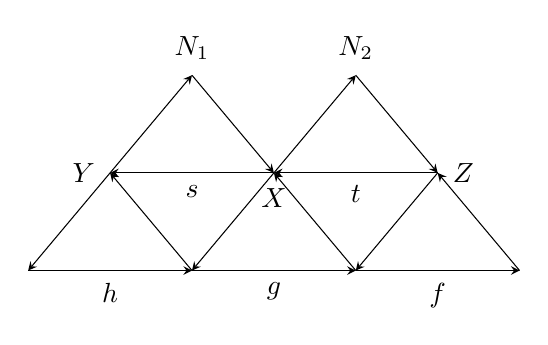
\begin{tikzpicture}[>=stealth,line width=.38pt,scale=.80]
    \coordinate (Y)  at (0,0);
    \coordinate (X)  at (2.6,0);
    \coordinate (Z)  at (5.2,0);
    \coordinate (N1) at (1.3,1.55);
    \coordinate (N2) at (3.9,1.55);
    \coordinate (A)  at (-1.3,-1.55);
    \coordinate (Q1) at (1.3,-1.55);
    \coordinate (Q2) at (3.9,-1.55);
    \coordinate (B)  at (6.5,-1.55);

    \VerdierHatchTriangle{Y}{N1}{X}
    \VerdierHatchTriangle{X}{N2}{Z}
    \VerdierHatchTriangle{Y}{A}{Q1}
    \VerdierHatchTriangle{X}{Q1}{Q2}
    \VerdierHatchTriangle{Z}{Q2}{B}

    \draw[->] (Y) -- (N1);
    \draw[->] (N1) -- (X);
    \draw[->] (X) -- node[below=1pt] {$s$} (Y);
    \draw[->] (X) -- (N2);
    \draw[->] (N2) -- (Z);
    \draw[->] (Z) -- node[below=1pt] {$t$} (X);

    \draw[->] (Y) -- (A);
    \draw[->] (A) -- node[below=1pt] {$h$} (Q1);
    \draw[->] (Q1) -- (Y);
    \draw[->] (X) -- (Q1);
    \draw[->] (Q1) -- node[below=1pt] {$g$} (Q2);
    \draw[->] (Q2) -- (X);
    \draw[->] (Z) -- (Q2);
    \draw[->] (Q2) -- node[below=1pt] {$f$} (B);
    \draw[->] (B) -- (Z);

    \node[left=2pt]  at (Y)  {$Y$};
    \node[below=2pt] at (X)  {$X$};
    \node[right=2pt] at (Z)  {$Z$};
    \node[above=2pt] at (N1) {$N_1$};
    \node[above=2pt] at (N2) {$N_2$};
  \end{tikzpicture}
  \quad ,
\end{center}

\VerdierSemanticAnchor{ch2-2-1-13-diagram-interpretation}
\noindent ここで $N_1$ と $N_2$ は $\mathcal D'$ の対象であり、網掛けされた
五つの三角は完全三角、網掛けされていない二つの三角は可換である。

\VerdierSemanticAnchor{ch2-2-1-13-shifted-zero}
したがって $s[1]t=0$ (1.2.2)。
\VerdierSemanticAnchor{ch2-2-1-13-shifted-membership}%
さらに SM1)、SM5) により、射 $s[1]t$ は $S(\mathcal D')$ に属する。

\VerdierSemanticAnchor{ch2-2-1-13-split-triangle}
ゆえに $N$ が $\mathcal D'$ の対象であるような形
$(Z,Y[2],N,0,u,v)$ の完全三角が存在する。
\VerdierSemanticAnchor{ch2-2-1-13-direct-summand}%
(1.2.6)、TRII により $Y$ は $\mathcal D'$ のある対象の直和因子である。
\VerdierSemanticAnchor{ch2-2-1-13-y-in-dprime}%
よって $Y$ は $\mathcal D'$ の対象と同型である。

\VerdierSemanticAnchor{ch2-2-1-13-s-triangle}
(1.2.4)、$\mathcal D'$ が $\mathcal D$ の三角部分圏であること、および完全三角

\begin{center}
  \begin{tikzpicture}[>=stealth,line width=.38pt,scale=.80]
    \coordinate (Y)  at (-2,0);
    \coordinate (X)  at (2,0);
    \coordinate (N1) at (0,1.55);
    \VerdierHatchTriangle{Y}{N1}{X}
    \draw[->] (Y) -- (N1);
    \draw[->] (N1) -- (X);
    \draw[->] (X) -- node[below=1pt] {$s$} (Y);
    \node[left=2pt]  at (Y)  {$Y$};
    \node[right=2pt] at (X)  {$X$};
    \node[above=2pt] at (N1) {$N_1$};
  \end{tikzpicture}
\end{center}

\VerdierSemanticAnchor{ch2-2-1-13-g-membership}
\noindent から、$X$ が $\mathcal D'$ の対象と同型であると分かる。したがって
射 $g$ は $S(\mathcal D')$ に属する。

\VerdierSemanticAnchor{ch2-2-1-14}
\medskip
\noindent\textbf{2.1.14.}\quad
\VerdierSemanticAnchor{ch2-2-1-14-saturation-direction}%
\emph{$S(\mathcal D')$ が飽和ならば $\mathcal D'$ は飽和である。}

\VerdierSemanticAnchor{ch2-2-1-14-direct-summand-setup}
$X$ を $\mathcal D'$ のある対象の直和因子とする。
\VerdierSemanticAnchor{ch2-2-1-14-first-triangle}%
(1.2.6)、TRII により、$N$ が $\mathcal D'$ の対象であるような完全三角
$(X,Y,N,0,u,v)$ が存在する。
\VerdierSemanticAnchor{ch2-2-1-14-zero-morphism}%
したがって零射 $X\to Y$ は $S(\mathcal D')$ に属する。

\VerdierSemanticAnchor{ch2-2-1-14-sm4-application}
三射 $0\to X\to 0\to Y$ に SM4) を適用する。
\VerdierSemanticAnchor{ch2-2-1-14-x-zero-membership}%
すると射 $X\to 0$ は $S(\mathcal D')$ に属する。

\VerdierSemanticAnchor{ch2-2-1-14-second-triangle}
ゆえに $N$ が $\mathcal D'$ の対象であるような完全三角
$(X,0,N,0,0,i)$ が存在する。
\VerdierSemanticAnchor{ch2-2-1-14-shift-isomorphism}%
したがって射 $N\xrightarrow{i}X[1]$ は同型で、$X$ は $N[-1]$ と同型であり、
後者は $\mathcal D'$ の対象である。

\VerdierSemanticAnchor{ch2-2-1-14-proposition-complete}
これで命題 (2.1.8) の証明が完了した。

\VerdierSemanticAnchor{ch2-2-1-14-p134-boundary}
\endgroup

\VerdierSourcePageBlock{0134}%
\begingroup
\VerdierSemanticAnchor{ch2-2-1-15}
\noindent\textbf{2.1.15.}\quad
\VerdierSemanticAnchor{ch2-2-1-15-associated-system}%
$\mathcal D'$ を三角圏 $\mathcal D$ の充満三角部分圏とする。乗法的系
$S(\mathcal D')$ (2.1.7) を、\emph{部分圏 $\mathcal D'$ に付随する
乗法的系}と呼ぶ。

\VerdierSemanticAnchor{ch2-2-1-16}
\smallskip
\noindent\textbf{命題 2.1.16.}\quad
\begingroup\itshape
\VerdierSemanticAnchor{ch2-2-1-16-setup}%
$F\colon\mathcal D_1\to\mathcal D_2$ を二つの三角圏の間の完全関手とする
(1.1.3)。$S(F)$ を、$F$ により $\mathcal D_2$ の同型へ送られる
$\mathcal D_1$ の射の集合とする。
\VerdierSemanticAnchor{ch2-2-1-16-kernel-subcategory}%
$\mathcal D'(F)$ を、$F$ により $\mathcal D_2$ の零対象へ送られる
$\mathcal D_1$ の対象で定まる $\mathcal D_1$ の充満部分圏とする。

\VerdierSemanticAnchor{ch2-2-1-16-a}
\par\noindent\hspace*{2em}a)\enspace 部分圏 $\mathcal D'(F)$ は厳密充満
三角部分圏（$\mathcal D'(F)$ の対象と同型な $\mathcal D_1$ の任意の
対象は $\mathcal D'(F)$ の対象である）であり、飽和である。

\VerdierSemanticAnchor{ch2-2-1-16-b}
\par\noindent\hspace*{2em}b)\enspace 集合 $S(F)$ は $\mathcal D_1$ の
飽和乗法的系である。

\VerdierSemanticAnchor{ch2-2-1-16-c}
\par\noindent\hspace*{2em}c)\enspace 集合 $S(F)$ は部分圏
$\mathcal D'(F)$ に付随する乗法的系である (2.1.15)。
\par\endgroup

\VerdierSemanticAnchor{ch2-2-1-16-proof-omitted}
\noindent 証明は容易なので読者に委ねる。同じ方法で次の命題も証明できる：

\VerdierSemanticAnchor{ch2-2-1-17}
\smallskip
\noindent\textbf{命題 2.1.17.}\quad
\begingroup\itshape
\VerdierSemanticAnchor{ch2-2-1-17-setup}%
$H\colon\mathcal D\to\mathcal A$ を三角圏からアーベル圏への
コホモロジー的関手とする。$S(H)$ を、$\mathcal D$ の射で、そのすべての
シフトとともに $\mathcal A$ の同型へ送られるものの集合とする。
\VerdierSemanticAnchor{ch2-2-1-17-kernel-subcategory}%
$\mathcal D'(H)$ を、$\mathcal D$ の対象で、そのすべてのシフトとともに
$\mathcal A$ の零対象へ送られるものによって定まる $\mathcal D$ の充満
部分圏とする。

\VerdierSemanticAnchor{ch2-2-1-17-a}
\par\noindent\hspace*{2em}a)\enspace 部分圏 $\mathcal D'(H)$ は厳密充満
三角部分圏であり、飽和である。

\VerdierSemanticAnchor{ch2-2-1-17-b}
\par\noindent\hspace*{2em}b)\enspace 集合 $S(H)$ は $\mathcal D$ の飽和
乗法的系である。

\VerdierSemanticAnchor{ch2-2-1-17-c}
\par\noindent\hspace*{2em}c)\enspace 集合 $S(H)$ は部分圏
$\mathcal D'(H)$ に付随する乗法的系である (2.1.15)。
\par\endgroup

\VerdierSemanticAnchor{ch2-2-2}
\medskip
\noindent\textbf{2.2.\quad 局所化圏の構成。}

\VerdierSemanticAnchor{ch2-2-2-1}
\smallskip
\noindent\textbf{2.2.1.}\quad
\VerdierSemanticAnchor{ch2-2-2-1-slice-categories}%
$\mathcal C$ を圏（加法的であるとは限らない）、$S$ を $\mathcal C$ の
乗法的系とする。$\mathcal C$ の各対象 $X$ に対し、$S/X$（それぞれ
$X\backslash S$）を、対象が終域 $X$（それぞれ始域 $X$）をもつ $S$
の射であり、
\VerdierSemanticAnchor{ch2-2-2-1-morphism-diagrams}%
射が次の可換図式であるような圏とする：

\VerdierSemanticAnchor{ch2-2-2-1-s-over-x-diagram}
\begin{center}
  \begin{tikzpicture}[>=stealth,line width=.38pt,scale=.90]
    \node (Y)  at (-1.55,1.05) {$Y$};
    \node (Yp) at ( 1.55,1.05) {$Y'$};
    \node (X)  at ( 0,-.95) {$X$};
    \draw[->] (Y) -- node[above=1pt] {$u$} (Yp);
    \draw[->] (Y) -- node[left=2pt] {$s$} (X);
    \draw[->] (Yp) -- node[right=2pt] {$t$} (X);
    \node at (3.15,.05) {$s,t\in S$};
  \end{tikzpicture}
  \quad ,
\end{center}

\VerdierSemanticAnchor{ch2-2-2-1-p135-boundary}
\endgroup%
\VerdierSourcePageContinue{0135}%
\begingroup
\normalsize
\setlength{\emergencystretch}{1.5em}%
\setlength{\abovedisplayskip}{2pt plus 1pt minus 1pt}%
\setlength{\belowdisplayskip}{2pt plus 1pt minus 1pt}%

\VerdierSemanticAnchor{ch2-2-2-1-x-backslash-s-diagram}
\noindent\hspace*{.3em}(それぞれ\quad
\begin{tikzpicture}[>=stealth,line width=.38pt,scale=.90,
  baseline={(current bounding box.center)}]
  \node (X)  at (0,1.50) {$X$};
  \node (Y)  at (-1.30,-.55) {$Y$};
  \node (Yp) at (1.30,-.55) {$Y'$};
  \draw[->] (X) -- node[left=2pt] {$s$} (Y);
  \draw[->] (X) -- node[right=2pt] {$t$} (Yp);
  \draw[->] (Y) -- node[above=1pt] {$u$} (Yp);
  \node at (3.10,.45) {$s,t\in S$};
\end{tikzpicture}
\quad )\,.

\VerdierSemanticAnchor{ch2-2-2-1-localized-hom-definition}
\smallskip
\noindent $\mathcal C$ の対象の各対 $X,Y$ に対し、次のようにおく：

\VerdierSemanticAnchor{ch2-2-2-1-formula-2-2-1-1}
\par\smallskip
\noindent\makebox[0pt][l]{(2.2.1.1)}%
\begin{minipage}[t]{\linewidth}
  \centering
  $\displaystyle
    \operatorname{Hom}_{\mathcal C(S^{-1})}(X,Y)
    =\varinjlim_{(S/X)^{\circ}}
     \operatorname{Hom}_{\mathcal C}(\,\cdot\,,Y)\,.$
\end{minipage}
\par\smallskip

\VerdierSemanticAnchor{ch2-2-2-1-dot-explanation}
\noindent （式 (2.2.1.1) の「点」は $S/X$ の可変対象の始域を表す。）

\VerdierSemanticAnchor{ch2-2-2-1-filtered-category}
性質 SM1)、SM2)、SM3) から、圏 $(S/X)^{\circ}$ がフィルター圏 [6]
であることが直ちに従う。
\VerdierSemanticAnchor{ch2-2-2-1-roof-class}%
したがって $\operatorname{Hom}_{\mathcal C(S^{-1})}(X,Y)$ の元は、次の形の
図式の同値類である：

\VerdierSemanticAnchor{ch2-2-2-1-roof-formula}
\[
  D=X\xleftarrow{s}X'\xrightarrow{m}Y,\qquad s\in S,
\]

\VerdierSemanticAnchor{ch2-2-2-1-equivalence-setup}
\noindent 二つの図式
$D_1=X\xleftarrow{s_1}X_1\xrightarrow{m_1}Y$ と
$D_2=X\xleftarrow{s_2}X_2\xrightarrow{m_2}Y$ が同じ同値類に属するための
必要十分条件は、次の図式が存在することである：

\VerdierSemanticAnchor{ch2-2-2-1-common-refinement-roof}
\[
  D_3=X\xleftarrow{s_3}X_3\xrightarrow{m_3}Y,\qquad s_3\in S,
\]

\VerdierSemanticAnchor{ch2-2-2-1-common-refinement-diagram-introduction}
\noindent および次の可換図式：

\VerdierSemanticAnchor{ch2-2-2-1-common-refinement-diagram}
\begin{center}
  \begin{tikzpicture}[>=stealth,line width=.38pt,x=1.45cm,y=1.02cm,
    scale=.95]
    \node (X1) at (0,1.35) {$X_1$};
    \node (X3) at (0,0) {$X_3$};
    \node (X2) at (0,-1.35) {$X_2$};
    \node (X)  at (-2.15,0) {$X$};
    \node (Y)  at (2.15,0) {$Y$};
    \draw[->] (X1) -- node[above left=-1pt] {$s_1$} (X);
    \draw[->] (X3) -- node[above=1pt] {$s_3$} (X);
    \draw[->] (X2) -- node[below left=-1pt] {$s_2$} (X);
    \draw[->] (X3) -- node[right=1pt] {$u$} (X1);
    \draw[->] (X3) -- node[right=1pt] {$v$} (X2);
    \draw[->] (X1) -- node[above right=-1pt] {$m_1$} (Y);
    \draw[->] (X3) -- node[above=1pt] {$m_3$} (Y);
    \draw[->] (X2) -- node[below right=-1pt] {$m_2$} (Y);
  \end{tikzpicture}
  \quad .
\end{center}

\VerdierSemanticAnchor{ch2-2-2-1-q-of-f}
\noindent 各元 $f\in\operatorname{Hom}_{\mathcal C}(X,Y)$ に対し、図式
$X\xleftarrow{\operatorname{id}_X}X\xrightarrow{f}Y$ の同値類を $Q(f)$
と書く。
\VerdierSemanticAnchor{ch2-2-2-1-q-of-s-inverse}%
各射 $s\colon Y\to X$、$s\in S$ に対し、図式
$X\xleftarrow{s}Y\xrightarrow{\operatorname{id}_Y}Y$ の同値類を
$Q(s)^{-1}$ と書く。

\VerdierSemanticAnchor{ch2-2-2-1-fl-morphism-set}
次に、$\operatorname{Fl}(\mathcal C(S^{-1}))$ により次の集合を表す：

\VerdierSemanticAnchor{ch2-2-2-1-fl-product-formula}
\[
  \prod_{(X,Y)\in\operatorname{Ob}(\mathcal C)\times\operatorname{Ob}(\mathcal C)}
  \operatorname{Hom}_{\mathcal C(S^{-1})}(X,Y),
\]

\VerdierSemanticAnchor{ch2-2-2-1-p136-boundary}
\endgroup%
\VerdierSourcePageContinue{0136}%
\begingroup
\VerdierSemanticAnchor{ch2-2-2-1-fl-source-target-maps}
\noindent $\mathbf{s}$ および $\mathbf{b}\colon
\operatorname{Fl}(\mathcal C(S^{-1}))\rightrightarrows
\operatorname{Ob}(\mathcal C)$ により次の写像を表す：

\VerdierSemanticAnchor{ch2-2-2-1-source-target-formula}
\[
  m\in\operatorname{Hom}_{\mathcal C(S^{-1})}(X,Y),\qquad
  \mathbf{s}(m)=X,\qquad \mathbf{b}(m)=Y,
\]

\VerdierSemanticAnchor{ch2-2-2-1-identity-map}
\noindent また $\mathbf{id}\colon\operatorname{Ob}(\mathcal C)
\to\operatorname{Fl}(\mathcal C(S^{-1}))$ により写像
$X\mapsto Q(\mathbf{id}_X)$ を表す。
\VerdierSemanticAnchor{ch2-2-2-1-category-diagram}%
こうして図式
\[
\mathcal C(S^{-1})=(\operatorname{Ob}(\mathcal C),
\operatorname{Fl}(\mathcal C(S^{-1})),\mathbf{s},\mathbf{b},\mathbf{id})
\]
を定める。さらに、記号を濫用して次のように書く写像の対がある：

\VerdierSemanticAnchor{ch2-2-2-1-q-pair}
\[
  Q=\bigl(\mathbf{id}_{\operatorname{Ob}(\mathcal C)}\colon
  \operatorname{Ob}(\mathcal C)\to\operatorname{Ob}(\mathcal C),\;
  Q\colon\operatorname{Fl}(\mathcal C)\to
  \operatorname{Fl}(\mathcal C(S^{-1}))\bigr)\,.
\]

\VerdierSemanticAnchor{ch2-2-2-2}
\smallskip
\noindent\textbf{定理 2.2.2.}\quad
\begingroup\itshape
\VerdierSemanticAnchor{ch2-2-2-2-a}%
a) $\operatorname{Fl}(\mathcal C(S^{-1}))$ 上には、次を満たす部分的に
定義された合成則がただ一つ存在する：

\VerdierSemanticAnchor{ch2-2-2-2-a-1}
\par\noindent\hspace*{2em}1) $\mathcal C(S^{-1})$ は圏である。

\VerdierSemanticAnchor{ch2-2-2-2-a-2}
\par\noindent\hspace*{2em}2) $Q(s)$ は同型であり、$Q(s)^{-1}$ はその逆
$(s\in S)$ である。

\VerdierSemanticAnchor{ch2-2-2-2-a-3}
\par\noindent\hspace*{2em}3) 各図式
$D=X\xleftarrow{s}X'\xrightarrow{m}Y$、$s\in S$ に対し、
$\overline D=Q(m)Q(s)^{-1}$ が成り立つ
$(\overline D\in\operatorname{Hom}_{\mathcal C(S^{-1})}(X,Y)$ は $D$ の
同値類である）。

\VerdierSemanticAnchor{ch2-2-2-2-a-4}
\par\noindent\hspace*{2em}4) $Q$ は関手である。

\VerdierSemanticAnchor{ch2-2-2-2-b}
\par\noindent b) $\mathcal C(S^{-1})$ の各射は合成
$Q(t)^{-1}Q(m)$、$m\in\operatorname{Fl}(\mathcal C)$、$t\in S$
（それぞれ $Q(p)Q(s)^{-1}$、$p\in\operatorname{Fl}(\mathcal C)$、
$s\in S$）と書ける。

\VerdierSemanticAnchor{ch2-2-2-2-c}
\par\noindent c) 関手 $Q$ は有限射影極限および有限帰納極限と可換である。

\VerdierSemanticAnchor{ch2-2-2-2-d}
\par\noindent d) 各圏 $\mathcal A$ に対し、関手 $Q$ との合成は関手

\VerdierSemanticAnchor{ch2-2-2-2-hom-q-a}
\[
  \mathcal{H}\!om(Q,\mathcal A)\colon
  \mathcal{H}\!om(\mathcal C(S^{-1}),\mathcal A)
  \longrightarrow \mathcal{H}\!om(\mathcal C,\mathcal A)
\]

\noindent\textup{を定める（$\mathcal{H}\!om$ は関手圏を表す）。}
\VerdierSemanticAnchor{ch2-2-2-2-universal-image}%
関手 $\mathcal{H}\!om(Q,\mathcal A)$ は対象上単射かつ充満忠実であり、
$\mathcal{H}\!om(\mathcal C(S^{-1}),\mathcal A)$ の像は、$S$ の射を
同型へ送る $\mathcal C$ から $\mathcal A$ への関手によって定まる
$\mathcal{H}\!om(\mathcal C,\mathcal A)$ の厳密充満部分圏である。
\par\endgroup

\VerdierSemanticAnchor{ch2-2-2-2-proof-omitted}
この定理の証明は読者に委ねる。[16] を参照してもよい。
\VerdierSemanticAnchor{ch2-2-2-2-composition-setup}%
ここでは $\mathcal C(S^{-1})$ における射の合成を記述するにとどめる。
$\overline D_1\in\operatorname{Hom}_{\mathcal C(S^{-1})}(X,Y)$ と
$\overline D_2\in\operatorname{Hom}_{\mathcal C(S^{-1})}(Y,Z)$ を
$\mathcal C(S^{-1})$ の合成可能な二射とする。

\VerdierSemanticAnchor{ch2-2-2-2-roof-pair}
$D_1=X\xleftarrow{s}X'\xrightarrow{m}Y$ と
$D_2=Y\xleftarrow{t}Y'\xrightarrow{p}Z$ を、それぞれ同値類
$\overline D_1$ と $\overline D_2$ に属する $\mathcal C$ の二図式とする。
\VerdierSemanticAnchor{ch2-2-2-2-sm2-completion-input}%
SM2) を用いて、次の図式を補完する：

\begin{center}
  \begin{tikzpicture}[>=stealth,line width=.38pt,x=1.42cm,y=.90cm,
    scale=.92]
    \node (Xp) at (-1.20,1.10) {$X'$};
    \node (Yp) at ( 1.20,1.10) {$Y'$};
    \node (Y)  at ( 0,-.70) {$Y$};
    \draw[->] (Xp) -- node[left=2pt] {$m$} (Y);
    \draw[->] (Yp) -- node[right=2pt] {$t$} (Y);
    \node at (3.00,.25) {$t\in S$};
  \end{tikzpicture}
\end{center}

\VerdierSemanticAnchor{ch2-2-2-2-p137-boundary}
\endgroup%
\VerdierSourcePageContinue{0137}%
\begingroup
\VerdierSemanticAnchor{ch2-2-2-2-sm2-completion-diagram}
\noindent 次の可換図式に補完する：

\begin{center}
  \begin{tikzpicture}[>=stealth,line width=.38pt,x=1.30cm,y=1.45cm,
    scale=.92]
    \node (Zpp) at (0,2.20) {$Z''$};
    \node (Xp)  at (-1.25,1.10) {$X'$};
    \node (Yp)  at ( 1.25,1.10) {$Y'$};
    \node (Y)   at (0,0) {$Y$};
    \draw[->] (Zpp) -- node[above left=-1pt] {$t'\in S$} (Xp);
    \draw[->] (Zpp) -- node[above right=-1pt] {$m'$} (Yp);
    \draw[->] (Xp)  -- node[below left=-1pt] {$m$} (Y);
    \draw[->] (Yp)  -- node[below right=-1pt] {$t\in S$} (Y);
    \node at (2.50,-.05) {$.$};
  \end{tikzpicture}
\end{center}

\VerdierSemanticAnchor{ch2-2-2-2-composite-roof-d3}
\noindent このとき図式
$D_3=X\xleftarrow{st'}Z''\xrightarrow{pm'}Z$ を得る。合成 $st'$ は
$S$ に属する (SM1)。
\VerdierSemanticAnchor{ch2-2-2-2-composite-class-independence}%
$D_3$ の $\operatorname{Hom}_{\mathcal C(S^{-1})}(X,Z)$ における同値類
$\overline D_3$ は、同値類 $\overline D_1$ と $\overline D_2$ のみに
依存することが分かる。
\VerdierSemanticAnchor{ch2-2-2-2-composition-conclusion}%
射 $\overline D_3$ は $\mathcal C(S^{-1})$ における射
$\overline D_1$ と $\overline D_2$ の合成である。

\VerdierSemanticAnchor{ch2-2-2-3}
\smallskip
\noindent\textbf{注意 2.2.3.}
\VerdierSemanticAnchor{ch2-2-2-3-a}%
a) 定理 (2.2.2) の第四の主張から、関手
$Q\colon\mathcal C\longrightarrow\mathcal C(S^{-1})$ を備えた圏
$\mathcal C(S^{-1})$ が次の普遍問題の解であることが従う：
\VerdierSemanticAnchor{ch2-2-2-3-a-universal-problem}%
関手 $Q$ はこの系の射を同型へ送り、$S$ の射を同型へ送る
$\mathcal C$ から任意の圏 $\mathcal A$ への各関手は $Q$ を通じて一意に
分解する。
\VerdierSemanticAnchor{ch2-2-2-3-a-unique-isomorphism}%
したがって、関手 $Q$ を備えた圏 $\mathcal C(S^{-1})$ は、この性質に
よって一意な同型を除いて決定される。

\VerdierSemanticAnchor{ch2-2-2-3-b}
\par\noindent b) $\mathcal C$ を圏、$S$ を $\mathcal C$ の射の集合とし、
$S$ が $\mathcal C$ の乗法的系であることは仮定しない。
\VerdierSemanticAnchor{ch2-2-2-3-b-general-localization}%
$S$ の射を同型へ送る圏 $\mathcal C(S^{-1})$ と関手
$Q\colon\mathcal C\longrightarrow\mathcal C(S^{-1})$ であって、$S$ の
射を同型へ送る $\mathcal C$ から任意の圏 $\mathcal A$ への各関手が
$Q$ を通じて一意に分解するものが常に存在する。
\VerdierSemanticAnchor{ch2-2-2-3-b-multiplicative-comparison}%
$S$ が $\mathcal C$ の乗法的系であるとき、定理 (2.2.2) は圏
$\mathcal C(S^{-1})$ の簡単な記述を与える。また、一般には成り立たない
関手 $Q$ の付加的性質（主張 b)、c)）も与える。

\VerdierSemanticAnchor{ch2-2-2-4}
\smallskip
\noindent\textbf{系 2.2.4.}\quad
\begingroup\itshape
$\mathcal C$ を圏、$S$ を $\mathcal C$ の乗法的系とする。

\VerdierSemanticAnchor{ch2-2-2-4-a}
\par\noindent a) 集合 $S$ は $\mathcal C$ の反対圏
$\mathcal C^\circ$ の乗法的系である。
\VerdierSemanticAnchor{ch2-2-2-4-a-opposite-system}%
次の標準的な圏の同型が存在する：

\VerdierSemanticAnchor{ch2-2-2-4-a-canonical-isomorphism}
\[
  \bigl(\mathcal C^\circ(S^{-1})\bigr)^\circ
  \longrightarrow \mathcal C(S^{-1})\,.
\]

\VerdierSemanticAnchor{ch2-2-2-4-a-hom-colimit-isomorphism}
\noindent 特に、この同型は次の同型を誘導する：
\[
  \operatorname{Hom}_{\mathcal C(S^{-1})}(X,Y)
  \longrightarrow
  \varinjlim_{Y\backslash S}\operatorname{Hom}_{\mathcal C}(X,\mathord\cdot)\,.
\]
\endgroup

\VerdierSemanticAnchor{ch2-2-2-4-p138-boundary}
\endgroup%
\VerdierSourcePageContinue{0138}%
\begingroup
\begingroup\itshape
\VerdierSemanticAnchor{ch2-2-2-4-b}
\noindent b) 圏 $\mathcal C$ が加法圏ならば、圏
$\mathcal C(S^{-1})$ は加法圏であり、関手 $Q$ は加法関手である。

\VerdierSemanticAnchor{ch2-2-2-4-c}
\par\noindent c) $\widehat S$ を、$Q$ により $\mathcal C(S^{-1})$ の
同型へ送られる $\mathcal C$ の射の集合とする。
\VerdierSemanticAnchor{ch2-2-2-4-c-saturation}%
集合 $\widehat S$ は $\mathcal C$ の飽和乗法的系である。$S$ を含む
$\mathcal C$ の任意の飽和乗法的系は $\widehat S$ を含む。
\endgroup

\VerdierSemanticAnchor{ch2-2-2-4-proof-b}
\par\noindent 第一の主張は $\mathcal C(S^{-1})$ の普遍性から直ちに従う：
圏 $\bigl(\mathcal C^\circ(S^{-1})\bigr)^\circ$ はこの問題の解である。
第二の主張は定理 (2.2.2) の主張 b)、c) から直ちに従う。
\VerdierSemanticAnchor{ch2-2-2-4-proof-c-characterization}%
$\mathcal C(S^{-1})$ の射の記述から、$\mathcal C$ の射 $f$ が $Q$ に
より同型へ送られるための必要十分条件は、$gf$ と $fh$ が定義されて
$S$ に属するような $\mathcal C$ の二射 $g$、$h$ が存在することだと
直ちに分かる。
\VerdierSemanticAnchor{ch2-2-2-4-proof-c-sm2-sm3}%
したがって、集合 $\widehat S$ は性質 SM2)、SM3) をもつ。
\VerdierSemanticAnchor{ch2-2-2-4-proof-c-sm1-sm4}%
さらに、$\widehat S$ の定義から、この集合は性質 SM1)、SM4) をもつ。
\VerdierSemanticAnchor{ch2-2-2-4-proof-c-conclusion}%
ゆえに $\widehat S$ は $\mathcal C$ の飽和乗法的系である。(2.2.4) の
最後の主張は明らかである。

\VerdierSemanticAnchor{ch2-2-2-5}
\smallskip
\noindent\textbf{2.2.5.} $\mathcal C$ を圏、$S$ を $\mathcal C$ の
乗法的系とする。
\VerdierSemanticAnchor{ch2-2-2-5-localized-category}%
圏 $\mathcal C(S^{-1})$ を、系 $S$ に関する $\mathcal C$ の
\emph{局所化圏}と呼ぶ。
\VerdierSemanticAnchor{ch2-2-2-5-localization-functor}%
関手 $Q\colon\mathcal C\longrightarrow\mathcal C(S^{-1})$ を
\emph{局所化関手}と呼ぶ。
\VerdierSemanticAnchor{ch2-2-2-5-saturation}%
乗法的系 $\widehat S$ を系 $S$ の\emph{飽和化}と呼ぶ。

\VerdierSemanticAnchor{ch2-2-2-6}
\smallskip
\noindent\textbf{定理 2.2.6.}\quad
\begingroup\itshape
\VerdierSemanticAnchor{ch2-2-2-6-setup}%
$\mathcal D$ を三角圏、$S$ を $\mathcal D$ の乗法的系とする (2.1.4)。
$\mathcal D(S^{-1})$ を $\mathcal D$ の局所化圏、
$Q\colon\mathcal D\longrightarrow\mathcal D(S^{-1})$ を局所化関手とする。

\VerdierSemanticAnchor{ch2-2-2-6-a}
\par\noindent a) $\mathcal D(S^{-1})$ 上には、$Q$ が厳密な
$\mathbb Z$-関手となるような厳密な $\mathbb Z$-圏の構造がただ一つ
存在する。

\VerdierSemanticAnchor{ch2-2-2-6-b}
\par\noindent b) $\mathcal D(S^{-1})$ 上には、$Q$ が完全関手となる
ような三角構造がただ一つ存在する。この構造の完全三角は、
$\mathcal D$ の完全三角の $Q$ による像と同型な三角である。

\VerdierSemanticAnchor{ch2-2-2-6-c-factorization}
\par\noindent c) $S$ の射を同型へ送る、三角圏（それぞれアーベル圏）
への任意の完全（それぞれコホモロジー的）関手
$F\colon\mathcal D\longrightarrow\mathcal D'$ は、
$Q\colon\mathcal D\longrightarrow\mathcal D(S^{-1})$ を通じて完全
（それぞれコホモロジー的）関手
$G\colon\mathcal D(S^{-1})\longrightarrow\mathcal D'$ として一意に
分解する。
\VerdierSemanticAnchor{ch2-2-2-6-c-morphism-lifting}%
$F_1,F_2\colon\mathcal D\rightrightarrows\mathcal D'$ を $S$ の射を
同型へ送る二つの完全（それぞれコホモロジー的）関手とし、
$G_1,G_2\colon\mathcal D(S^{-1})\rightrightarrows\mathcal D'$ をそれぞれ
の分解、$m\colon F_1\longrightarrow F_2$ を完全（それぞれ
コホモロジー的）関手の射とする。このとき $m=p\star Q$ を満たす
関手の射 $p\colon G_1\longrightarrow G_2$ がただ一つ存在する。
\endgroup

\VerdierSemanticAnchor{ch2-2-2-6-proof-a}
\par\noindent 第一の主張は定理 (2.2.2) と SM5) から直ちに従う。
\VerdierSemanticAnchor{ch2-2-2-6-proof-c-p139-boundary}%
第三の主張は

\VerdierSemanticAnchor{ch2-2-2-6-p139-boundary}
\endgroup%
\VerdierSourcePageContinue{0139}%
\begingroup
\normalsize
\setlength{\parskip}{0pt}%
\setlength{\emergencystretch}{1.5em}%
\setlength{\abovedisplayskip}{1pt plus 1pt minus 1pt}%
\setlength{\belowdisplayskip}{1pt plus 1pt minus 1pt}%

\VerdierSemanticAnchor{ch2-2-2-6-proof-c-continuation}
\noindent 第二の主張と定理 (2.2.2) から直ちに従う。したがって第二の
主張を証明すればよい。
\VerdierSemanticAnchor{ch2-2-2-6-proof-b-setup}%
$T$ を、$\mathcal D$ の完全三角の $Q$ による像と同型な
$\mathcal D(S^{-1})$ の三角の集合とする。
\VerdierSemanticAnchor{ch2-2-2-6-proof-b-tri-trii}%
集合 $T$ が性質 TRI、TRII をもつことは容易に確かめられる。性質 TRIII
を示すには次の補題が必要である：

\VerdierSemanticAnchor{ch2-2-2-7}
\smallskip
\noindent\textbf{補題 2.2.7.}\quad
\begingroup\itshape
$u\colon X\longrightarrow Y$ と $u'\colon X'\longrightarrow Y'$ を
$\mathcal D$ の二射とし、

\VerdierSemanticAnchor{ch2-2-2-7-localized-square}
\begin{center}
  \begin{tikzpicture}[>=stealth,line width=.38pt,x=1.70cm,y=1.25cm,
    scale=.98]
    \node (QX)  at (0,1) {$Q(X)$};
    \node (QY)  at (2.35,1) {$Q(Y)$};
    \node (QXp) at (0,0) {$Q(X')$};
    \node (QYp) at (2.35,0) {$Q(Y')$};
    \draw[->] (QX) -- node[above] {$Q(u)$} (QY);
    \draw[->] (QXp) -- node[below] {$Q(u')$} (QYp);
    \draw[->] (QX) -- node[left] {$m$} (QXp);
    \draw[->] (QY) -- node[right] {$p$} (QYp);
  \end{tikzpicture}
\end{center}

\noindent を $\mathcal D(S^{-1})$ における可換図式とする。
\VerdierSemanticAnchor{ch2-2-2-7-common-representative}%
このとき射 $u''\colon X''\longrightarrow Y''$ と、$\mathcal D$ における
二つの可換図式

\begin{center}
  \VerdierSemanticAnchor{ch2-2-2-7-denominator-square}%
  \begin{tikzpicture}[>=stealth,line width=.38pt,x=1.55cm,y=1.15cm,
    scale=.95]
    \node (Xpp) at (0,1) {$X''$};
    \node (Ypp) at (2,1) {$Y''$};
    \node (X)   at (0,0) {$X$};
    \node (Y)   at (2,0) {$Y$};
    \draw[->] (Xpp) -- node[above] {$u''$} (Ypp);
    \draw[->] (X) -- node[below] {$u$} (Y);
    \draw[->] (Xpp) -- node[left] {$s$} (X);
    \draw[->] (Ypp) -- node[right] {$t$} (Y);
    \node at (3.25,.50) {$s,t\in S$};
    \node at (4.50,0) {$,$};
  \end{tikzpicture}
  \par\smallskip
  \VerdierSemanticAnchor{ch2-2-2-7-numerator-square}%
  \begin{tikzpicture}[>=stealth,line width=.38pt,x=1.55cm,y=1.15cm,
    scale=.95]
    \node (Xpp) at (0,1) {$X''$};
    \node (Ypp) at (2,1) {$Y''$};
    \node (Xp)  at (0,0) {$X'$};
    \node (Yp)  at (2,0) {$Y'$};
    \draw[->] (Xpp) -- node[above] {$u''$} (Ypp);
    \draw[->] (Xp) -- node[below] {$u'$} (Yp);
    \draw[->] (Xpp) -- node[left] {$f$} (Xp);
    \draw[->] (Ypp) -- node[right] {$g$} (Yp);
    \node at (3.10,0) {$,$};
  \end{tikzpicture}
\end{center}

\VerdierSemanticAnchor{ch2-2-2-7-fraction-identities}
\noindent であって、$m=Q(f)Q(s)^{-1}$、$p=Q(g)Q(t)^{-1}$ を満たす
ものが存在する。
\endgroup

\VerdierSemanticAnchor{ch2-2-2-6-proof-b-triii-reduction}
\par\noindent 補題を認め、集合 $T$ が性質 TRIII をもつことを示そう。
集合 $T$ の定義により、次を示せばよい：$\mathcal D$ の二つの完全三角

\VerdierSemanticAnchor{ch2-2-2-6-proof-b-distinguished-triangles}
\[
  (X,Y,Z,u,v,w)\,,\qquad
  (X',Y',Z',u',v',w')
\]

\noindent と、$\mathcal D(S^{-1})$ の可換図式

\VerdierSemanticAnchor{ch2-2-2-6-proof-b-localized-square}
\begin{center}
  \begin{tikzpicture}[>=stealth,line width=.38pt,x=1.70cm,y=1.25cm,
    scale=.98]
    \node (QX)  at (0,1) {$Q(X)$};
    \node (QY)  at (2.35,1) {$Q(Y)$};
    \node (QXp) at (0,0) {$Q(X')$};
    \node (QYp) at (2.35,0) {$Q(Y')$};
    \draw[->] (QX) -- node[above] {$Q(u)$} (QY);
    \draw[->] (QXp) -- node[below] {$Q(u')$} (QYp);
    \draw[->] (QX) -- node[left] {$m$} (QXp);
    \draw[->] (QY) -- node[right] {$p$} (QYp);
    \node at (3.05,0) {$,$};
  \end{tikzpicture}
\end{center}

\VerdierSemanticAnchor{ch2-2-2-6-proof-b-p140-boundary}
\VerdierSemanticAnchor{ch2-2-2-6-p140-boundary}
\endgroup%
\VerdierSourcePageContinue{0140}%
\begingroup
\normalsize
\setlength{\parskip}{0pt}%
\setlength{\emergencystretch}{1.5em}%
\setlength{\abovedisplayskip}{1pt plus 1pt minus 1pt}%
\setlength{\belowdisplayskip}{1pt plus 1pt minus 1pt}%

\VerdierSemanticAnchor{ch2-2-2-6-proof-b-triii-completion}
\noindent が与えられたとき、$(m,p,r)$ が三角の射となるような射
$r\colon Q(Z)\longrightarrow Q(Z')$ が存在する。
\VerdierSemanticAnchor{ch2-2-2-6-proof-b-triii-case-reduction}%
補題 (2.2.7) により、次の二つの場合を考えればよい：

\VerdierSemanticAnchor{ch2-2-2-6-proof-b-triii-case-a}
\noindent\textit{a)}\quad
$m=Q(s)^{-1}$、$p=Q(t)^{-1}$、$s,t\in S$ であり、図式

\VerdierSemanticAnchor{ch2-2-2-6-proof-b-triii-case-a-square}
\begin{center}
  \begin{tikzpicture}[>=stealth,line width=.38pt,x=1.85cm,y=1.45cm,
    scale=1.04]
    \node (Xp) at (0,1) {$X'$};
    \node (Yp) at (2,1) {$Y'$};
    \node (X)  at (0,0) {$X$};
    \node (Y)  at (2,0) {$Y$};
    \draw[->] (Xp) -- node[above] {$u'$} (Yp);
    \draw[->] (Xp) -- node[left] {$s$} (X);
    \draw[->] (Yp) -- node[right] {$t$} (Y);
    \draw[->] (X) -- node[below] {$u$} (Y);
  \end{tikzpicture}
\end{center}

\noindent は可換である。

\VerdierSemanticAnchor{ch2-2-2-6-proof-b-triii-case-b}
\noindent\textit{b)}\quad
$m=Q(f)$、$p=Q(g)$ であり、図式

\VerdierSemanticAnchor{ch2-2-2-6-proof-b-triii-case-b-square}
\begin{center}
  \begin{tikzpicture}[>=stealth,line width=.38pt,x=1.85cm,y=1.45cm,
    scale=1.04]
    \node (X)  at (0,1) {$X$};
    \node (Y)  at (2,1) {$Y$};
    \node (Xp) at (0,0) {$X'$};
    \node (Yp) at (2,0) {$Y'$};
    \draw[->] (X) -- node[above] {$u$} (Y);
    \draw[->] (X) -- node[left] {$f$} (Xp);
    \draw[->] (Y) -- node[right] {$g$} (Yp);
    \draw[->] (Xp) -- node[below] {$u'$} (Yp);
  \end{tikzpicture}
\end{center}

\noindent は可換である。

\VerdierSemanticAnchor{ch2-2-2-6-proof-b-triii-case-conclusion}
\noindent 場合 \textit{a)} では、主張は性質 SM6) (2.1.2) から従う。
場合 \textit{b)} では、$\mathcal D$ の完全三角に対する性質 TRIII から
従う。

\VerdierSemanticAnchor{ch2-2-2-8}
\smallskip
\noindent\textbf{2.2.8.\quad 補題 2.2.7 の証明。}
\VerdierSemanticAnchor{ch2-2-2-8-initial-lift}%
定理 (2.2.2) により、$pQ(t)=Q(g)$ を満たす射
$t\colon Y''\longrightarrow Y$、$t\in S$ が存在する。ただし
$g\colon Y''\longrightarrow Y'$ である。次の図式を段階的に構成する：

\VerdierSemanticAnchor{ch2-2-2-8-stepwise-diagram}
\begin{center}
  \begin{tikzpicture}[>=stealth,line width=.38pt,x=1.80cm,y=1.45cm,
    scale=1.04]
    \node (Xpp)  at (0,3) {$X''$};
    \node (X2pp) at (0,2) {$X_2''$};
    \node (X1pp) at (0,1) {$X_1''$};
    \node (X)    at (0,0) {$X$};
    \node (Ypp)  at (2.35,1) {$Y''$};
    \node (Y)    at (2.35,0) {$Y$};
    \draw[->] (Xpp) -- node[left] {$s_3$} (X2pp);
    \draw[->] (X2pp) -- node[left] {$s_2$} (X1pp);
    \draw[->] (X1pp) -- node[left] {$s_1$} (X);
    \draw[->] (Xpp) -- node[pos=.58,above right] {$u''$} (Ypp);
    \draw[->] (X2pp) -- node[pos=.58,above] {$u_2''$} (Ypp);
    \draw[->] (X1pp) -- node[below] {$u_1''$} (Ypp);
    \draw[->] (Ypp) -- node[right] {$t$} (Y);
    \draw[->] (X) -- node[below] {$u$} (Y);
    \node at (3.15,0) {$,$};
  \end{tikzpicture}
\end{center}

\VerdierSemanticAnchor{ch2-2-2-8-proof-p141-boundary}
\VerdierSemanticAnchor{ch2-2-2-8-p141-boundary}
\endgroup%
\VerdierSourcePageContinue{0141}%
\begingroup
\VerdierSemanticAnchor{ch2-2-2-8-stepwise-conditions}
\noindent ただし次を満たす：

\VerdierSemanticAnchor{ch2-2-2-8-condition-1}
\par\noindent\makebox[1.8em][l]{1)}$us_1=tu_1''$ かつ $s_1\in S$。
これは SM2) を用いて得られる。

\VerdierSemanticAnchor{ch2-2-2-8-condition-2}
\par\noindent\makebox[1.8em][l]{2)}$mQ(s_1s_2)=Q(f')$。ただし
$f'\colon X_2''\longrightarrow X'$ は $\mathcal D$ の射、
$u_2''=u_1''s_2$、$s_2\in S$ である。これは定理 (2.2.2) を用いて
得られる。

\VerdierSemanticAnchor{ch2-2-2-8-condition-3}
\par\noindent\makebox[1.8em][l]{3)}$u'f's_3=gu_2''s_3$、
$u''=u_2''s_3$、$s_3\in S$。実際、$\mathcal D$ の図式

\VerdierSemanticAnchor{ch2-2-2-8-source-square}
\begin{center}
  \begin{tikzpicture}[>=stealth,line width=.38pt,x=1.85cm,y=1.10cm,
    scale=.96]
    \node (X2pp) at (0,1) {$X_2''$};
    \node (Ypp)  at (2,1) {$Y''$};
    \node (Xp)   at (0,0) {$X'$};
    \node (Yp)   at (2,0) {$Y'$};
    \draw[->] (X2pp) -- node[above] {$u_2''$} (Ypp);
    \draw[->] (X2pp) -- node[left] {$f'$} (Xp);
    \draw[->] (Ypp)  -- node[right] {$g$} (Yp);
    \draw[->] (Xp)   -- node[below] {$u'$} (Yp);
  \end{tikzpicture}
\end{center}

\VerdierSemanticAnchor{ch2-2-2-8-localized-commutativity}
\noindent は必ずしも可換ではない。しかし、この図式に関手 $Q$ を
適用して得られる $\mathcal D(S^{-1})$ の図式は可換である。したがって
$Q(u'f')=Q(gu_2'')\colon Q(X_2'')\longrightarrow Q(Y')$ である。

\VerdierSemanticAnchor{ch2-2-2-8-s3-refinement}
$\mathcal D(S^{-1})$ の射の定義により、$u'f's_3=gu_2''s_3$ を満たす射
$s_3\in S\colon X''\longrightarrow X_2''$ が存在する。

\VerdierSemanticAnchor{ch2-2-2-8-proof-complete}
補題の証明を完了するには $f=f's_3$、$s=s_1s_2s_3$ とおけばよい。

\VerdierSemanticAnchor{ch2-2-2-9}
\smallskip
\noindent\textbf{2.2.9. 定理 2.2.6 の証明の完了。}
\VerdierSemanticAnchor{ch2-2-2-9-triv-reduction}%
集合 $T$ が性質 TRIV をもつことを示せばよい。この集合は性質 TRI、
TRII、TRIII をもつことが既に分かっているので、1.2 の結果 (1.2.14)
を用いてよい。特に (1.2.4) により、与えられた射を含む $T$ の三角は
すべて同型である。したがって、命題 (1.3.2) の証明で用いたものと
同様の簡約により、性質 TRIV の証明は、$\mathcal D$ の類似の図式を
$Q$ で写して得られる $\mathcal D(S^{-1})$ の図式に帰着される。

\VerdierSemanticAnchor{ch2-2-2-9-reader-details}
この検証は容易である。詳細は読者に委ねる。

\VerdierSemanticAnchor{ch2-2-2-10}
\smallskip
\noindent\textbf{2.2.10.}\quad
$\mathcal D$ を三角圏、$\mathcal B\subseteq\mathcal D$ を充満三角部分圏、
$S(\mathcal B)$ を $\mathcal B$ に付随する乗法的系とする (2.1.15)。

\VerdierSemanticAnchor{ch2-2-2-10-quotient-category}
圏 $\mathcal D(S(\mathcal B)^{-1})$ を $\mathcal D/\mathcal B$ と書く。
圏 $\mathcal D/\mathcal B$ を\emph{$\mathcal B$ による $\mathcal D$ の
商圏}と呼ぶ。

\VerdierSemanticAnchor{ch2-2-2-10-quotient-functor}
標準関手 $Q\colon\mathcal D\longrightarrow\mathcal D/\mathcal B$ を
\emph{商関手}と呼ぶ。$F\colon\mathcal D\longrightarrow\mathcal D'$ を
三角圏（それぞれアーベル圏）への完全（それぞれコホモロジー的）関手
とする。

\VerdierSemanticAnchor{ch2-2-2-10-kernel}
$F$ により零対象へ送られる対象（それぞれ、そのすべてのシフトが
$F$ により零対象へ送られる対象）によって定まる厳密充満飽和三角部分圏を
$\operatorname{Ker}(F)$ と書き、\emph{$F$ の核}と呼ぶ
（(2.1.16)、(2.1.17)）。

\VerdierSemanticAnchor{ch2-2-2-10-p142-boundary}
\endgroup

\VerdierSourcePageBlock{0142}%
\begingroup
\VerdierSemanticAnchor{ch2-2-2-11}
\noindent\textbf{系 2.2.11.}\quad
\begingroup\itshape
\VerdierSemanticAnchor{ch2-2-2-11-setup}%
$\mathcal D$ を三角圏、$\mathcal B\subset\mathcal D$ を充満三角部分圏
とする。

\VerdierSemanticAnchor{ch2-2-2-11-a}
\par\noindent a) 商関手
$Q\colon\mathcal D\longrightarrow\mathcal D/\mathcal B$ の核は、
$\mathcal B$ を含む最小の厳密充満飽和三角部分圏である。

\VerdierSemanticAnchor{ch2-2-2-11-b-order-isomorphism}
\par\noindent b) 各厳密充満飽和三角部分圏にその飽和乗法的系 (2.1.8)
を対応させる写像 $\mathcal B\longmapsto S(\mathcal B)$ は、包含関係で
順序づけた厳密充満飽和三角部分圏の集合から、包含関係で順序づけた
$\mathcal D$ の飽和乗法的系の集合への順序集合の同型である。

\VerdierSemanticAnchor{ch2-2-2-11-b-inverse}
逆写像は、各飽和乗法的系に対応する局所化関手の核を対応させる。

\VerdierSemanticAnchor{ch2-2-2-11-c-factorization}
\par\noindent c) 核が部分圏 $\mathcal B$ を含む完全（それぞれ
コホモロジー的）関手 $F\colon\mathcal D\longrightarrow\mathcal D'$ は、
$Q\colon\mathcal D\longrightarrow\mathcal D/\mathcal B$ を通じて完全
（それぞれコホモロジー的）関手
$G\colon\mathcal D/\mathcal B\longrightarrow\mathcal D'$ として一意に
分解する。

\VerdierSemanticAnchor{ch2-2-2-11-c-morphism-lifting}
核が部分圏 $\mathcal B$ を含む完全（それぞれコホモロジー的）関手の射は、
それらの分解の間の射から一意に生じる。
\endgroup

\VerdierSemanticAnchor{ch2-2-2-11-easy-consequences}
これらは定理 (2.2.6) から容易に従う。

\VerdierSemanticAnchor{ch2-2-2-12}
\smallskip
\noindent\textbf{2.2.12. 性質 TRIV に関する注意。}
\VerdierSemanticAnchor{ch2-2-2-12-pretriangulated-category}%
性質 TRI、TRII、TRIII を満たす三角の族を備えた厳密な
$\mathbb Z$-圏を\emph{前三角圏}と呼ぶことにする。

\VerdierSemanticAnchor{ch2-2-2-12-induced-notions}
\emph{完全関手}、\emph{コホモロジー的関手}、\emph{乗法的系}の概念を、
三角圏の場合と同様に定義する。

\VerdierSemanticAnchor{ch2-2-2-12-localization}
$\mathcal D$ を前三角圏、$S$ をその乗法的系とする (2.1.4)。局所化圏
$\mathcal D(S^{-1})$ 上には、局所化関手が完全となるような前三角圏の
構造がただ一つ存在する。

\VerdierSemanticAnchor{ch2-2-2-12-kernel-subcategory}
局所化関手により零化される $\mathcal D$ の対象からなる充満部分圏は、
充満前三角部分圏である。

\VerdierSemanticAnchor{ch2-2-2-12-triv-necessity}
実際には、逆に、前三角部分圏に適切な飽和乗法的系を対応させる方法を
知る必要がある。編者が知る方法は性質 TRIV を用いるものだけである。

\VerdierSemanticAnchor{ch2-2-2-12-triv-role}
したがって、この本質的にかなり技術的な性質は、これまでのところ主に
定理 (2.2.6) から系 (2.2.11) を導くために用いられた。

\VerdierSemanticAnchor{ch2-2-3}
\medskip
\noindent\textbf{2.3. 局所化関手の性質。}

\VerdierSemanticAnchor{ch2-2-3-1}
\smallskip
\noindent\textbf{命題 2.3.1.}\quad
\itshape $\mathcal D$ を三角圏、$\mathcal B$ を充満三角部分圏とする。\upshape

\VerdierSemanticAnchor{ch2-2-3-1-p143-boundary}
\endgroup%
\VerdierSourcePageContinue{0143}%
\begingroup
\begingroup\itshape
\VerdierSemanticAnchor{ch2-2-3-1-continuation}%
$\mathcal B\subset\mathcal A\subset\mathcal D$ を満たす任意の充満三角部分圏
$\mathcal A$ に対し、$\mathcal B$ に対応する $\mathcal D$（それぞれ
$\mathcal A$）の乗法的系を $S_{\mathcal D}(\mathcal B)$（それぞれ
$S_{\mathcal A}(\mathcal B)$）と書く (2.1.7)。

\VerdierSemanticAnchor{ch2-2-3-1-a-intersection}
\par\noindent a) 次が成り立つ：
$S_{\mathcal D}(\mathcal B)\cap\operatorname{Fl}(\mathcal A)
=S_{\mathcal A}(\mathcal B)$。

\VerdierSemanticAnchor{ch2-2-3-1-b-fully-faithful}
\par\noindent b) 標準関手
$\mathcal A/\mathcal B\longrightarrow\mathcal D/\mathcal B$ は充満忠実で、
対象上単射である。この関手の像は $Q(\mathcal A)$ である。ここで
$Q\colon\mathcal D\longrightarrow\mathcal D/\mathcal B$ は標準関手である。

\VerdierSemanticAnchor{ch2-2-3-1-c-quotient-transitivity}
\par\noindent c) 標準関手
$\mathcal D/\mathcal A\longrightarrow
(\mathcal D/\mathcal B)/(\mathcal A/\mathcal B)$ は圏の同型である。

\VerdierSemanticAnchor{ch2-2-3-1-d-saturation}
\par\noindent d) 圏 $\mathcal A$ が飽和ならば (2.1.6)、部分圏
$Q(\mathcal A)$ は飽和である。

\VerdierSemanticAnchor{ch2-2-3-1-inverse-image-setup}
$\mathcal D/\mathcal B$ の任意の充満三角部分圏 $\mathcal C$ に対し、
$Q(X)$ が圏 $\mathcal C$ のある対象と同型になるような $\mathcal D$ の
対象 $X$ からなる $\mathcal D$ の充満部分圏を $Q^{-1}(\mathcal C)$ と書く。

\VerdierSemanticAnchor{ch2-2-3-1-a-bis}
\par\noindent a)$^{\mathrm{bis}}$ 圏 $Q^{-1}(\mathcal C)$ は
$\mathcal D$ の厳密充満三角部分圏である。

\VerdierSemanticAnchor{ch2-2-3-1-b-bis}
\par\noindent b)$^{\mathrm{bis}}$ 乗法的系
$S_{\mathcal D}(Q^{-1}(\mathcal C))$ は、$Q$ による像が
$S_{\mathcal D/\mathcal B}(\mathcal C)$ の射となる $\mathcal D$ の射から
なる。

\VerdierSemanticAnchor{ch2-2-3-1-c-bis}
\par\noindent c)$^{\mathrm{bis}}$ 部分圏 $Q^{-1}(\mathcal C)$ が飽和である
ための必要十分条件は、部分圏 $\mathcal C$ が飽和であることである。

\VerdierSemanticAnchor{ch2-2-3-1-d-bis}
\par\noindent d)$^{\mathrm{bis}}$ 写像
$\mathcal A\longmapsto Q(\mathcal A)$ は、包含関係で順序づけた、
$\widehat{\mathcal B}$（関手 $Q$ の核）を含む $\mathcal D$ の厳密充満
三角部分圏の集合から、包含関係で順序づけた $\mathcal D/\mathcal B$ の
厳密充満三角部分圏の集合への順序集合の同型である。逆写像は
$\mathcal C\longmapsto Q^{-1}(\mathcal C)$ である。
\endgroup

\VerdierSemanticAnchor{ch2-2-3-1-proof-ab}
第一の主張は明らかである。第二の主張は、圏 $\mathcal A/\mathcal B$ と
$\mathcal D/\mathcal B$ における射の記述 (2.2.1) から直ちに従う。

\VerdierSemanticAnchor{ch2-2-3-1-proof-c}
c) を示すには、商圏の普遍性 (2.2.11) を参照すればよい。

\VerdierSemanticAnchor{ch2-2-3-1-proof-d}
d) を示そう。$\mathcal A$ をその厳密充満閉包で置き換えても
$Q(\mathcal A)$ は同値の範囲でしか変わらないので、$\mathcal A$ は厳密充満
であると仮定してよい。このとき関手
$\mathcal D\longrightarrow\mathcal D/\mathcal A$ の核は圏 $\mathcal A$
である (2.2.11)。この関手は
$\mathcal D\longrightarrow\mathcal D/\mathcal B
\longrightarrow\mathcal D/\mathcal A$ と分解する。したがって標準関手
$\mathcal D/\mathcal B\longrightarrow\mathcal D/\mathcal A$ の核は
$Q(\mathcal A)$ である。ゆえに $Q(\mathcal A)$ は飽和である (2.1.16)。

\VerdierSemanticAnchor{ch2-2-3-1-proof-a-bis-b-bis}
主張 a)$^{\mathrm{bis}}$ は明らかであり、主張 b)$^{\mathrm{bis}}$ も同様で
ある。

\VerdierSemanticAnchor{ch2-2-3-1-proof-c-bis-forward}
$\mathcal C$ が飽和であると仮定する。さらに $\mathcal C$ は厳密充満で
あると仮定してよい。実際、$\widehat{\mathcal C}$ を $\mathcal C$ の厳密充満
閉包とすると、圏 $\widehat{\mathcal C}$ は厳密充満かつ飽和であり、
$Q^{-1}(\widehat{\mathcal C})=Q^{-1}(\mathcal C)$ である。このとき圏
$\mathcal C$ はある完全関手の核である (2.2.11)。したがって
$Q^{-1}(\mathcal C)$ はある完全関手の核であり、ゆえに飽和である
(2.1.16)。

\VerdierSemanticAnchor{ch2-2-3-1-p144-boundary}
$Q^{-1}(\mathcal C)$ が
\endgroup%
\VerdierSourcePageContinue{0144}%
\begingroup
\VerdierSemanticAnchor{ch2-2-3-1-proof-c-bis-converse}
\noindent 飽和である。d) の証明により、部分圏
$Q(Q^{-1}(\mathcal C))$ は厳密充満かつ飽和である。一方、圏
$Q(Q^{-1}(\mathcal C))$ は $\mathcal C$ の厳密充満閉包である。したがって
$\mathcal C$ は飽和である。これで主張 c)$^{\mathrm{bis}}$ が示された。

\VerdierSemanticAnchor{ch2-2-3-1-proof-d-bis}
最後の主張を示す。$\mathcal C$ が厳密充満ならば
$Q(Q^{-1}(\mathcal C))=\mathcal C$ であることは明らかである。
$\widehat{\mathcal B}$ を含む厳密充満三角圏 $\mathcal A$ をとる。
$\mathcal A=Q^{-1}(Q(\mathcal A))$ を示せばよい。$\mathcal B$ を
$\widehat{\mathcal B}$ で置き換えても圏 $\mathcal D/\mathcal B$ は変わらない
(2.2.11) ので、$\mathcal B$ は飽和で
$\mathcal B=\widehat{\mathcal B}$ と仮定してよい。包含
$\mathcal A\subset Q^{-1}(Q(\mathcal A))$ は明らかなので、
$\mathcal D/\mathcal B$ で $\mathcal A$ の対象と同型になる
$\mathcal D$ の任意の対象が $\mathcal A$ の対象であることを示せばよい。

\VerdierSemanticAnchor{ch2-2-3-1-proof-d-bis-roof-setup}
$X$ を $\mathcal A$ の対象、$Y$ を $\mathcal D$ の対象とし、同型
$m\colon Q(X)\xrightarrow{\sim}Q(Y)$ をとる。射 $m$ は
$m=Q(f)Q(s)^{-1}$ と分解でき、ここで
$s\in S_{\mathcal D}(\mathcal B)$ (2.2.2)、$Q(f)$ は同型である。
$\mathcal B$ は飽和なので $f\in S_{\mathcal D}(\mathcal B)$ である
（(2.1.8) と (2.2.4)）。したがって $\mathcal D$ に次の図式がある：

\VerdierSemanticAnchor{ch2-2-3-1-proof-d-bis-roof}
\begin{center}
  \begin{tikzcd}[column sep=4.2em,row sep=2.5em,baseline=(current bounding box.center)]
    & Z \arrow[dl,"s"'] \arrow[dr,"f"] & \\
    X && Y
  \end{tikzcd}
  \qquad $s,f\in S_{\mathcal D}(\mathcal B)$\quad .
\end{center}

\VerdierSemanticAnchor{ch2-2-3-1-proof-d-bis-complete}
$s$ は $S_{\mathcal D}(\mathcal B)$ に属するので、$W$ が $\mathcal B$ の対象である
完全三角 $(Z,X,W,s,u,v)$ が存在する (2.1.7)。したがって $W$ は
$\mathcal A$ の対象であり、$\mathcal A$ は厳密充満だから $Z$ も
$\mathcal A$ の対象である (1.2.4)。同じ議論により $Y$ も
$\mathcal A$ の対象となり、命題の証明が完了する。

\VerdierSemanticAnchor{ch2-2-3-2}
\medskip\noindent\textbf{2.3.2.}\quad
\VerdierSemanticAnchor{ch2-2-3-2-free-object}
$F\colon C\longrightarrow C'$ を関手、$X$ を $C'$ の対象とする。
$u\colon F(Y)\longrightarrow X$ が存在し、任意の射
$F(Z)\xrightarrow{v}X$ に対して下図を可換にする唯一の射
$w\colon Z\longrightarrow Y$ が存在するとき、$C$ の対象 $Y$ は
\emph{$X$ 上 $F$-右自由}、または単に\emph{$X$ 上右自由}であるという：

\VerdierSemanticAnchor{ch2-2-3-2-free-object-diagram}
\begin{center}
  \begin{tikzcd}[column sep=4.7em,row sep=2.7em]
    F(Y) \arrow[rr,"u"] && X \\
    & F(Z) \arrow[ul,"{F(w)}"] \arrow[ur,"v"'] &
  \end{tikzcd}
  \quad .
\end{center}

\VerdierSemanticAnchor{ch2-2-3-2-freedom-arrow-boundary}
矢 $u\colon F(Y)\longrightarrow X$ を、組 $(X,Y)$ の（関手 $F$ に関する）
\emph{自由矢}という。これはまた、ある
\endgroup%
\VerdierSourcePageContinue{0145}%
\begingroup
\VerdierSemanticAnchor{ch2-2-3-2-free-object-continuation}
\noindent $C$ と $C'$ を要素として含む宇宙をとれば、関手
$Z\longmapsto\operatorname{Hom}_C(Z,Y)$ と
$Z\longmapsto\operatorname{Hom}_{C'}(F(Z),X)$ の間に同型が存在するとき
$Y$ は $X$ 上右自由である、と言い換えられる。

\VerdierSemanticAnchor{ch2-2-3-2-right-left-terminology}
$C'$ の対象 $X$ が存在して $Y$ が $X$ 上右自由となるとき、$C$ の対象
$Y$ は\emph{$F$-右自由}であるという。$X$ 上右自由な $C$ の対象 $Y$ が
存在するとき、$C'$ の対象 $X$ は\emph{$F$-右自由化可能}である
という。反対圏へ移ることで、\emph{左}自由および左自由化可能な対象も同様に
定義する。

\VerdierSemanticAnchor{ch2-2-3-3}
\medskip\begingroup\itshape
\noindent\textbf{命題 2.3.3.}\quad
$\mathcal D$ を三角圏、$\mathcal B$ を充満三角部分圏、
$Q\colon\mathcal D\longrightarrow\mathcal D/\mathcal B$ を商関手
(2.2.10)、$S_{\mathcal D}(\mathcal B)$ を $\mathcal B$ に対応する
$\mathcal D$ の乗法的系 (2.1.8) とする。

\VerdierSemanticAnchor{ch2-2-3-3-a}
\par\noindent a) $\mathcal D$ の任意の対象 $Y$ に対し、次の条件は同値である：
\VerdierSemanticAnchor{ch2-2-3-3-a-i}
\par\noindent\hspace{1.2em}i) 対象 $Y$ は $Q$-右自由である。
\VerdierSemanticAnchor{ch2-2-3-3-a-ii}
\par\noindent\hspace{1.2em}ii) 任意の射
$s\in S_{\mathcal D}(\mathcal B)$、$s\colon S\longrightarrow T$ に対し、写像
\[
  \operatorname{Hom}_{\mathcal D}(s,Y)\colon
  \operatorname{Hom}_{\mathcal D}(T,Y)\longrightarrow
  \operatorname{Hom}_{\mathcal D}(S,Y)
\]
は全単射である。
\VerdierSemanticAnchor{ch2-2-3-3-a-iii}
\par\noindent\hspace{1.2em}iii) $\mathcal B$ の任意の対象 $B$ に対し、
$\operatorname{Hom}_{\mathcal D}(B,Y)=0$。
\VerdierSemanticAnchor{ch2-2-3-3-a-iv}
\par\noindent\hspace{1.2em}iv) $s\in S_{\mathcal D}(\mathcal B)$ である
任意の射 $Y\xrightarrow{s}Z$ はレトラクションをもつ。
\VerdierSemanticAnchor{ch2-2-3-3-a-v}
\par\noindent\hspace{1.2em}v) $\mathcal D$ の任意の対象 $X$ に対し、写像
\[
  \operatorname{Hom}_{\mathcal D}(X,Y)\longrightarrow
  \operatorname{Hom}_{\mathcal D/\mathcal B}(Q(X),Q(Y))
\]
は全単射である。

\VerdierSemanticAnchor{ch2-2-3-3-b}
\par\noindent b) $L_R(Q)$ を $Q$-右自由な対象で定まる $\mathcal D$ の充満
部分圏とする。圏 $L_R(Q)$ は三角圏であり、厳密充満かつ飽和である。
\VerdierSemanticAnchor{ch2-2-3-3-c}
\par\noindent c) 商関手の $L_R(Q)$ への制限
\[
  Q|_{L_R(Q)}\colon L_R(Q)\longrightarrow\mathcal D/\mathcal B
  ,
\]
は充満忠実で、対象上単射である。
\VerdierSemanticAnchor{ch2-2-3-3-d}
\par\noindent d) $\operatorname{Lib}_R(Q)\subset\mathcal D/\mathcal B$ を
$\mathcal D/\mathcal B$ の $Q$-右自由化可能な対象で定まる充満部分圏とする。
$\operatorname{Lib}_R(Q)$ は厳密充満三角部分圏である。可算積または可算直和が
$\mathcal D$ で表現可能ならば、$\operatorname{Lib}_R(Q)$ は飽和である。
\VerdierSemanticAnchor{ch2-2-3-3-e}
\par\noindent e) 関手 $Q$ は $L_R(Q)$ を $\operatorname{Lib}_R(Q)$ に送る。
$\operatorname{Lib}_R(Q)$ は $L_R(Q)$ の像の厳密充満閉包である。自由矢は
同型である。
\endgroup
\endgroup%
\VerdierSourcePageContinue{0146}%
\begingroup
\sloppy

\begingroup\itshape
\VerdierSemanticAnchor{ch2-2-3-3-f}
\noindent f) $\mathcal D$ の対象 $Z$ が
$Q^{-1}(\operatorname{Lib}_R(Q))$ に属するための必要十分条件は、右自由な対象
$Y$ と射 $s\colon Z\longrightarrow Y$ が存在し、
$s$ が $\widehat{S_{\mathcal D}(\mathcal B)}$ に属することである。ここで後者は
$S_{\mathcal D}(\mathcal B)$ の飽和化である (2.2.4, (c))。
\VerdierSemanticAnchor{ch2-2-3-3-g}
\par\noindent g) 包含関手
$L_R(Q)\subset Q^{-1}(\operatorname{Lib}_R(Q))$ は左随伴
\[
  \mathcal R\colon Q^{-1}(\operatorname{Lib}_R(Q))\longrightarrow L_R(Q)
  .
\]
をもつ。
\VerdierSemanticAnchor{ch2-2-3-3-adjunction-diagram}
\begin{center}
\begin{tikzcd}[column sep=3.2em,row sep=3.1em]
L_R(Q) \arrow[r,shift left=.7ex] \arrow[dr,"{Q|_{L_R(Q)}}"'] &
Q^{-1}(\operatorname{Lib}_R(Q))
 \arrow[l,dashed,bend right=28,"{\mathcal R}"'] \arrow[r,hook]
 \arrow[d,"{Q_1}"] & \mathcal D \arrow[d,"Q"] \\
& \operatorname{Lib}_R(Q) \arrow[ul,dashed,bend left=10,"{\Psi}"']
 \arrow[r,hook] & \mathcal D/\mathcal B
\end{tikzcd}
\end{center}
\endgroup

\VerdierSemanticAnchor{ch2-2-3-3-adjunction-explanation}
$\Psi\colon\operatorname{Lib}_R(Q)\longrightarrow L_R(Q)$ を
$Q|_{L_R(Q)}$ の擬逆関手とする（c), e) 参照）。
$\mathcal R=\Psi Q_1$ ととれる。ここで
$Q_1\colon Q^{-1}(\operatorname{Lib}_R(Q))\longrightarrow
\operatorname{Lib}_R(Q)$ は $Q$ から誘導される関手である。関手 $\Psi$ は
関手 $Q_1$ の右随伴である。

\VerdierSemanticAnchor{ch2-2-3-4}
\medskip\noindent\textbf{2.3.4. 命題 2.3.3 の証明：}\quad
\VerdierSemanticAnchor{ch2-2-3-4-a-proof}
a) を示す。まず $Y$ が $Q$-右自由ならば、関手
$X\longmapsto\operatorname{Hom}_{\mathcal D}(X,Y)$ は、
$\mathcal D/\mathcal B$ の適当な対象 $Z$ に対する関手
$X\longmapsto\operatorname{Hom}_{\mathcal D/\mathcal B}(Q(X),Z)$ と同型で
ある。よって関手 $X\longmapsto\operatorname{Hom}_{\mathcal D}(X,Y)$ は
$S_{\mathcal D}(\mathcal B)$ の射を同型に送る。これで
i) $\Rightarrow$ ii) が従う。ii) $\Rightarrow$ iii) は
$B\longrightarrow0$ が $S_{\mathcal D}(\mathcal B)$ に属することから従い、iii)
$\Rightarrow$ iv) は $S_{\mathcal D}(\mathcal B)$ の定義と (1.2.6) から
従う。iv) $\Rightarrow$ v) は次の同型 (2.2.4) から従う：
\VerdierSemanticAnchor{ch2-2-3-4-colimit-isomorphism}
\[
  \operatorname{Hom}_{\mathcal D/\mathcal B}(Q(X),Q(Y))
  \xrightarrow{\sim}
  \varinjlim_{Y\backslash S_{\mathcal D}(\mathcal B)}
  \operatorname{Hom}_{\mathcal D}(X,\mathord\cdot)\, .
\]
\VerdierSemanticAnchor{ch2-2-3-4-a-proof-complete}
最後に v) $\Rightarrow$ i) は明らかである。実際、$Y$ は $Q(Y)$ 上
右自由である。
\VerdierSemanticAnchor{ch2-2-3-4-b-c-e-proof}
b) は a), iii) から、c) は a), v) から従う。さらに a), v) により、
$\mathcal D/\mathcal B$ の右自由化可能な対象は、$\mathcal D/\mathcal B$ で
$Q$-右自由な対象の $Q$ による像と同型な $\mathcal D/\mathcal B$ の対象に
ほかならない。自由矢は同型で
ある。これで e) が従い、$\operatorname{Lib}_R(Q)$ は厳密充満三角部分圏で
あることも明らかである。
\VerdierSemanticAnchor{ch2-2-3-4-d-proof}
$Z=Z_1\oplus Z_2$ を $\operatorname{Lib}_R(Q)$ の対象とする。
$Q$-右自由な対象 $Y$ と同型 $Q(Y)\xrightarrow{\sim}Z_1\oplus Z_2$ が
存在する。したがって関手 $X\longmapsto\operatorname{Hom}_{\mathcal D}(X,Y)$
は射影子をもち、$Z$ の直和分解は $Y$ 上の射影子を定める。$Z$ の直和因子が
$\operatorname{Lib}_R(Q)$ に属するための必要十分条件はこの射影子が分解可能
であることであり、可算直和または可算積が $\mathcal D$ で表現可能ならば
そうなる (1.2.9)。
\endgroup

\VerdierSourcePageBlock{0147}%
\begingroup
\VerdierSemanticAnchor{ch2-2-3-4-d-complete}
\noindent これで d) が示された。次に f) を示す。
\VerdierSemanticAnchor{ch2-2-3-4-f}
$\mathcal D$ の対象 $Z$ が $Q^{-1}(\operatorname{Lib}_R(Q))$ に属するための
必要十分条件は、$Q$-右自由な対象 $Y$ と $\mathcal D/\mathcal B$ における
同型 $Q(Z)\xrightarrow[\sim]{m}Q(Y)$ が存在することである。
\VerdierSemanticAnchor{ch2-2-3-4-f-fraction}
この同型は $m=Q(s)^{-1}Q(t)$ と書ける。ここで
$s\in S_{\mathcal D}(\mathcal B)$、
$t\in\widehat{S_{\mathcal D}(\mathcal B)}$ である（(2.2.2) と
(2.2.4)）。よって $\mathcal D$ に次の図式がある：
\VerdierSemanticAnchor{ch2-2-3-4-f-diagram}
\begin{center}
 \begin{tikzcd}[column sep=4.1em,row sep=2.5em]
 Z \arrow[r,"t"] & X & Y \arrow[l,"s"']
 \end{tikzcd}\quad .
\end{center}
\VerdierSemanticAnchor{ch2-2-3-4-f-retraction}
a), iv) により、$s$ は $S_{\mathcal D}(\mathcal B)$ に属するレトラクション
$s'\colon X\longrightarrow Y$ をもつ (1.2.6)。したがって
$t'\colon Z\longrightarrow Y$、$t'\in\widehat{S_{\mathcal D}(\mathcal B)}$
が存在する。
\VerdierSemanticAnchor{ch2-2-3-4-f-converse}
逆にこのような射が存在すれば $Q(t')\colon Q(Z)\longrightarrow Q(Y)$ は
同型である。
\VerdierSemanticAnchor{ch2-2-3-4-g}
残る g) を示す。a), v) により双関手的同型
\VerdierSemanticAnchor{ch2-2-3-4-g-q1-adjunction}
\[
 \operatorname{Hom}_{Q^{-1}(\operatorname{Lib}_R(Q))}(Z,\Psi(W))
 \xrightarrow{\sim}
 \operatorname{Hom}_{\operatorname{Lib}_R(Q)}(Q_1(Z),W),
\]
があり、$\Psi$ は $Q_1$ の右随伴である。
\VerdierSemanticAnchor{ch2-2-3-4-g-inclusion-adjunction}
したがって包含関手を $i\colon L_R(Q)\lhook\joinrel\longrightarrow
Q^{-1}(\operatorname{Lib}_R(Q))$ と書けば、双関手的同型
\[
 \operatorname{Hom}_{Q^{-1}(\operatorname{Lib}_R(Q))}(Z,i(Y))
 \xrightarrow{\sim}
 \operatorname{Hom}_{L_R(Q)}(\Psi Q_1(Z),Y)\, .
\]
を得る。
\VerdierSemanticAnchor{ch2-2-3-4-g-proof-complete}
これは $\mathcal R=\Psi Q_1$ が包含関手の左随伴であることを示し、命題
(2.3.3) の証明を完了する。

\begingroup\itshape
\VerdierSemanticAnchor{ch2-2-3-5}
\medskip\noindent\textbf{命題 2.3.5.}\quad
\VerdierSemanticAnchor{ch2-2-3-5-setup}
$\mathcal D$ を三角圏、$\mathcal A$ と $\mathcal B$ を二つの充満三角部分圏
（$\mathcal B$ は厳密充満）とし、$S_{\mathcal D}(\mathcal B)$ と
$S_{\mathcal A}(\mathcal A\cap\mathcal B)$ をそれぞれ $\mathcal B$ と
$\mathcal A\cap\mathcal B$ に対応する $\mathcal D$ と $\mathcal A$ の
乗法的系とする。
\VerdierSemanticAnchor{ch2-2-3-5-a}
\par\noindent a) 次の条件は同値である：
\VerdierSemanticAnchor{ch2-2-3-5-a-i}
\par\noindent\hspace{1.2em}i) $X\in\operatorname{Ob}(\mathcal A)$、
$s\in S_{\mathcal D}(\mathcal B)$ である任意の射
$X\xrightarrow{s}X'$ は次の可換図式に組み込まれる：
\VerdierSemanticAnchor{ch2-2-3-5-a-i-diagram}
\begin{center}
 \begin{tikzcd}[column sep=4.1em,row sep=2.6em]
 X \arrow[r,"s"] \arrow[dr,"{s'}"'] & X' \arrow[d] &
 {s'\in S_{\mathcal A}(\mathcal A\cap\mathcal B)} \\
 & X'' &
 \end{tikzcd}\quad .
\end{center}
\endgroup
\endgroup%
\VerdierSourcePageContinue{0148}%
\begingroup
\begingroup\itshape
\VerdierSemanticAnchor{ch2-2-3-5-a-ii}
\noindent\hspace{1.2em}ii) $B\in\operatorname{Ob}(\mathcal B)$、
$X\in\operatorname{Ob}(\mathcal A)$ である任意の射 $B\longrightarrow X$ は
次の可換図式に組み込まれる：
\VerdierSemanticAnchor{ch2-2-3-5-a-ii-diagram}
\begin{center}
 \begin{tikzcd}[column sep=4.2em,row sep=2.6em]
 B \arrow[r] \arrow[dr] & X & {B'\in\operatorname{Ob}(\mathcal A\cap\mathcal B)} \\
 & B' \arrow[u] &
 \end{tikzcd}\quad .
\end{center}
\VerdierSemanticAnchor{ch2-2-3-5-a-definition}
上の二つの同値な性質をもつ $\mathcal D$ の充満三角部分圏 $\mathcal A$ を
\emph{右 $\mathcal B$-局所化部分圏}という。
\VerdierSemanticAnchor{ch2-2-3-5-b}
\par\noindent b) $\mathcal A$ が右 $\mathcal B$-局所化ならば、標準関手
\VerdierSemanticAnchor{ch2-2-3-5-b-functor}
\[
 \mathcal A/(\mathcal A\cap\mathcal B)\longrightarrow\mathcal D/\mathcal B
\]
は充満忠実で、対象上単射である。
\VerdierSemanticAnchor{ch2-2-3-5-c}
\par\noindent c) 次の条件は同値である：
\VerdierSemanticAnchor{ch2-2-3-5-c-i}
\par\noindent\hspace{1.2em}i) $\mathcal A$ は右 $\mathcal B$-局所化である。
\VerdierSemanticAnchor{ch2-2-3-5-c-ii}
\par\noindent\hspace{1.2em}ii) 標準関手
$Q\colon\mathcal D/(\mathcal A\cap\mathcal B)\longrightarrow
\mathcal D/\mathcal B$ に対し、部分圏
$\mathcal A/(\mathcal A\cap\mathcal B)\longrightarrow
\mathcal D/(\mathcal A\cap\mathcal B)$ は $Q$-右自由な対象からなる。
\endgroup

\VerdierSemanticAnchor{ch2-2-3-5-proof-a}
a) の同値性は TRIII と乗法的系 $S_{\mathcal D}(\mathcal B)$、
$S_{\mathcal A}(\mathcal A\cap\mathcal B)$ の定義 (2.1.7) から直ちに従う。
\VerdierSemanticAnchor{ch2-2-3-5-proof-b-setup}
b) を示す。$X$ と $Y$ を $\mathcal A$ の二対象（したがって
$\mathcal A/(\mathcal A\cap\mathcal B)$ の対象）とする。
\VerdierSemanticAnchor{ch2-2-3-5-proof-b-injectivity}
まず準同型
\[
 \operatorname{Hom}_{\mathcal A/(\mathcal A\cap\mathcal B)}(X,Y)
 \longrightarrow\operatorname{Hom}_{\mathcal D/\mathcal B}(X,Y)
\]
が単射であることを示す。
\VerdierSemanticAnchor{ch2-2-3-5-proof-b-quotient-functors}
$Q_1\colon\mathcal A\longrightarrow\mathcal A/(\mathcal A\cap\mathcal B)$ と
$Q_2\colon\mathcal D\longrightarrow\mathcal D/\mathcal B$ を標準商関手とする。
\VerdierSemanticAnchor{ch2-2-3-5-proof-b-fraction}
任意の元 $m\in\operatorname{Hom}_{\mathcal A/(\mathcal A\cap\mathcal B)}(X,Y)$
は $m=Q_1(s)^{-1}Q_1(f)$、
$s\in S_{\mathcal A}(\mathcal A\cap\mathcal B)$ と書ける (2.2.2)。その
$\operatorname{Hom}_{\mathcal D/\mathcal B}(X,Y)$ における像は
$Q_2(s)^{-1}Q_2(f)$ である。
\VerdierSemanticAnchor{ch2-2-3-5-proof-b-zero-criterion}
(2.2.4, a)) により、この像が零となるための必要十分条件は次の可換図式が
存在することである：
\VerdierSemanticAnchor{ch2-2-3-5-proof-b-zero-diagram}
\begin{center}
 \begin{tikzcd}[column sep=3.7em,row sep=2.5em]
 & {} \arrow[r,"u"] & {} \\
 X \arrow[ur,"f"] && Y \arrow[ul,"s"] \arrow[u,"t"'] &
 {t\in S_{\mathcal D}(\mathcal B)}
 \end{tikzcd}
\end{center}
\endgroup%
\VerdierSourcePageContinue{0149}%
\begingroup
\sloppy

\VerdierSemanticAnchor{ch2-2-3-5-injectivity-p149-continuation}
\noindent かつ $uf=0$ となる。a), i) を用いると、さらに可換図式
\VerdierSemanticAnchor{ch2-2-3-5-injectivity-refinement-diagram}
\begin{center}
 \begin{tikzcd}[column sep=3.7em,row sep=2.3em]
 && {} \\
 & {} \arrow[ur,"v"] && {t'\in S_{\mathcal A}(\mathcal A\cap\mathcal B)} \\
 X \arrow[ur,"f"] && Y \arrow[ul,"s"] \arrow[uu,"{t'}"'] &
 \end{tikzcd}
\end{center}
\VerdierSemanticAnchor{ch2-2-3-5-injectivity-conclusion}
\noindent が存在して $vf=0$ となる。したがって
$m=Q_1(t')^{-1}Q_1(vf)=0$ である。
\VerdierSemanticAnchor{ch2-2-3-5-surjectivity-map}
次に準同型
\[
 \operatorname{Hom}_{\mathcal A/(\mathcal A\cap\mathcal B)}(X,Y)
 \longrightarrow\operatorname{Hom}_{\mathcal D/\mathcal B}(X,Y)
\]
が全射であることを示す。
\VerdierSemanticAnchor{ch2-2-3-5-surjectivity-roof}
任意の元 $p\in\operatorname{Hom}_{\mathcal D/\mathcal B}(X,Y)$ は
\[
 p=Q_2(t)^{-1}Q_2(g),\qquad t\in S_{\mathcal D}(\mathcal B)
  .
\]
と書ける。
\VerdierSemanticAnchor{ch2-2-3-5-surjectivity-refinement}
a), i) により、この元は常に
\[
 p=Q_2(s)^{-1}Q_2(g'),\qquad
 s\in S_{\mathcal A}(\mathcal A\cap\mathcal B),
\]
と書ける。
\VerdierSemanticAnchor{ch2-2-3-5-surjectivity-conclusion}
したがって $\operatorname{Hom}_{\mathcal A/(\mathcal A\cap\mathcal B)}(X,Y)$
の元から来る。
\VerdierSemanticAnchor{ch2-2-3-5-c-proof-i-implies-ii}
残る c) の同値性を示す。まず i) $\Rightarrow$ ii) を示す。
\VerdierSemanticAnchor{ch2-2-3-5-iterated-quotient}
(2.3.1) により $\mathcal D/\mathcal B$ は標準的に
$(\mathcal D/(\mathcal A\cap\mathcal B))
/(\mathcal B/(\mathcal A\cap\mathcal B))$ と同型であり、標準関手
\VerdierSemanticAnchor{ch2-2-3-5-q-functor}
\[
 Q\colon\mathcal D/(\mathcal A\cap\mathcal B)\longrightarrow\mathcal D/\mathcal B
\]
は商関手である。
\VerdierSemanticAnchor{ch2-2-3-5-q-free-reduction}
よって命題 (2.3.3, a)) により、i) $\Rightarrow$ ii) を示すには、
$\mathcal A$ の任意の対象 $X$ と
$\mathcal B$ の任意の対象 $B$ に対して
$\operatorname{Hom}_{\mathcal D/(\mathcal A\cap\mathcal B)}(B,X)=0$ を
示せばよい。
\VerdierSemanticAnchor{ch2-2-3-5-m-representation}
$\operatorname{Hom}_{\mathcal D/(\mathcal A\cap\mathcal B)}(B,X)$ の任意の元
$m$ は $Q_3(f)Q_3(s)^{-1}$ と書ける。ここで
\VerdierSemanticAnchor{ch2-2-3-5-q3-functor}
\[
 Q_3\colon\mathcal D\longrightarrow\mathcal D/(\mathcal A\cap\mathcal B)
\]
は標準関手であり、$s$ は $S_{\mathcal D}(\mathcal A\cap\mathcal B)$ に属し、後者は
$\mathcal A\cap\mathcal B$ に対応する $\mathcal D$ の乗法的系である
(2.2.2)。よって $\mathcal D$ に次の図式がある：
\VerdierSemanticAnchor{ch2-2-3-5-w-diagram}
\begin{center}
 \begin{tikzcd}[column sep=4em,row sep=2.4em]
 & W \arrow[dl,"s"'] \arrow[dr,"f"] & \\
 B && X
 \end{tikzcd}\quad ,
\end{center}
\endgroup%
\VerdierSourcePageContinue{0150}%
\begingroup
\VerdierSemanticAnchor{ch2-2-3-5-w-continuation}
\noindent $B$ は $\mathcal B$ の対象であり、$s$ は
$S_{\mathcal D}(\mathcal A\cap\mathcal B)$ に属するので、$W$ は
$\mathcal B$ のある対象と同型である (1.2.4)。
\VerdierSemanticAnchor{ch2-2-3-5-i-implies-ii-conclusion}
したがって第一の主張により、$f$ は $\mathcal A\cap\mathcal B$ の対象を
経由して分解する。ゆえに $Q_3(f)$ は零であり、したがって $m=0$ である。
\VerdierSemanticAnchor{ch2-2-3-5-ii-implies-i}
次に ii) $\Rightarrow$ i) を示す。a) により、$B$ が $\mathcal B$ の対象、
$X$ が $\mathcal A$ の対象である $\mathcal D$ の任意の射
$g\colon B\longrightarrow X$ が $\mathcal A\cap\mathcal B$ の対象を経由して
分解することを示せばよい。
\VerdierSemanticAnchor{ch2-2-3-5-q3-g-zero}
仮定により
$Q_3(g)\in\operatorname{Hom}_{\mathcal D/(\mathcal A\cap\mathcal B)}(B,X)$
は零である。
\VerdierSemanticAnchor{ch2-2-3-5-t-morphism}
よって (2.2.4) により、$t\in S_{\mathcal D}(\mathcal A\cap\mathcal B)$
かつ $tg=0$ となる射 $t\colon X\longrightarrow X'$ が存在する。
\VerdierSemanticAnchor{ch2-2-3-5-distinguished-triangle}
$S_{\mathcal D}(\mathcal A\cap\mathcal B)$ の定義により、$B'$ が
$\mathcal A\cap\mathcal B$ の対象である形 $(B',X,X',i,t,w)$ の
$\mathcal D$ の完全三角が存在する。
\VerdierSemanticAnchor{ch2-2-3-5-proof-complete}
(1.2.1) により $tg=0$ から $g$ は $B'$ を経由して分解する。これで命題
(2.3.5) の証明が完了する。
\VerdierSemanticAnchor{ch2-2-3-5-left-localizing-definition}
\medskip
$\mathcal D^\circ$ の部分圏 $\mathcal A^\circ$ が右
$\mathcal B^\circ$-局所化であるとき、$\mathcal D$ の充満三角部分圏
$\mathcal A$ は\emph{左 $\mathcal B$-局所化}であるという。
\endgroup

\VerdierSourcePageSilent{0151}%

\clearpage
\VerdierSourcePageBlock{0152}%
\begingroup
\VerdierSemanticAnchor{ch3}
\section{三角圏のアーベル化。}

\VerdierSemanticAnchor{ch3-3-1}
\subsection{圏 \texorpdfstring{$\mathrm A(\mathcal D)$}{A(D)} の構成。}

\VerdierSemanticAnchor{ch3-3-1-1}
\noindent\textbf{3.1.1.}\quad
$\mathcal D$ を加法圏とし、$\mathcal{F}\ell_1(\mathcal D)$ を
$\mathcal D$ の射の圏とする（第 I 章，3.3.6）。次の可換図式を考える：

\VerdierSemanticAnchor{ch3-3-1-1-square}
\[
\begin{tikzcd}[column sep=4.2em,row sep=2.5em]
X \arrow[r,"f"] \arrow[d,"g"'] & Y \arrow[d,"h"] \\
X' \arrow[r,"f'"'] & Y'
\end{tikzcd}
\]

\VerdierSemanticAnchor{ch3-3-1-1-negligible-morphism}
\noindent この $\mathcal{F}\ell_1(\mathcal D)$ の射が
$f'g=hf=0$ を満たすとき、
これを\emph{無視可能射}という。
無視可能射と任意の射との合成は、いずれの順序でも無視可能であり、二つの
無視可能射の直和も無視可能である。

\VerdierSemanticAnchor{ch3-3-1-1-quotient-category}
$\mathrm A(\mathcal D)$ を、対象が $\mathcal{F}\ell_1(\mathcal D)$ の対象で、
射が $\mathcal{F}\ell_1(\mathcal D)$ の射を無視可能射で割ったものである圏と
する。すなわち、$\mathrm A(\mathcal D)$ の対象 $U,V$ に対して
$\operatorname{Hom}_{\mathrm A(\mathcal D)}(U,V)$ は
$\operatorname{Hom}_{\mathcal{F}\ell_1(\mathcal D)}(U,V)$ を無視可能射の
部分群で割った商群である。圏 $\mathrm A(\mathcal D)$ は加法圏である。

\VerdierSemanticAnchor{ch3-3-1-1-canonical-quotient}
$C$ を圏とする。標準関手
\[
\mathcal{F}\ell_1(\mathcal D)\longrightarrow\mathrm A(\mathcal D)
\]
との合成により関手

\VerdierSemanticAnchor{ch3-3-1-1-1}
\[
\mathcal H\!om(\mathrm A(\mathcal D),C)
\longrightarrow
\mathcal H\!om(\mathcal{F}\ell_1(\mathcal D),C).
\tag{3.1.1.1}
\]
が得られる。この関手は充満忠実であり、対象上単射である。その像は、
無視可能射だけ異なる二つの射を同じ射に送る、
$\mathcal{F}\ell_1(\mathcal D)$ から $C$ への関手からなる充満部分圏である。

\VerdierSemanticAnchor{ch3-3-1-2}
\medskip
\noindent\textbf{3.1.2.}\quad
$\mathcal D$ から $\mathcal{F}\ell_1(\mathcal D)$ への標準関手
$X\longmapsto(X\xrightarrow{\operatorname{id}_X}X)$ と標準関手
$\mathcal{F}\ell_1(\mathcal D)\longrightarrow\mathrm A(\mathcal D)$ の合成を

\VerdierSemanticAnchor{ch3-3-1-2-1}
\[
\mathcal H\colon\mathcal D\longrightarrow\mathrm A(\mathcal D).
\tag{3.1.2.1}
\]
と書く。関手 $\mathcal H$ は加法的で、充満忠実かつ対象上単射である。
したがって $\mathcal D$ を $\mathrm A(\mathcal D)$ の充満部分圏として実現する。
\endgroup

\VerdierSourcePageBlock{0153}%
\begingroup
\VerdierSemanticAnchor{ch3-3-1-3}
\noindent\textbf{3.1.3.}\quad
$\mathcal D$ が厳密な $\mathbb Z$-圏であるとする。$\mathcal D$ のシフト関手
$X\longmapsto X[n]$（$n\in\mathbb Z$）は
$\mathcal{F}\ell_1(\mathcal D)$ の自己同型へ拡張される：

\VerdierSemanticAnchor{ch3-3-1-3-translation-extension}
\[
\bigl(X\xrightarrow{f}Y\bigr)
\longmapsto
\bigl(X[n]\xrightarrow{f[n]}Y[n]\bigr).
\]
$\mathrm A(\mathcal D)$ の普遍性 (3.1.1.1) から、これらの自己同型は商に
降下し、$\mathrm A(\mathcal D)$ に厳密な $\mathbb Z$-圏の構造を定める。
関手 $\mathcal H\colon\mathcal D\to\mathrm A(\mathcal D)$ は厳密な
$\mathbb Z$-関手である。

\VerdierSemanticAnchor{ch3-3-1-4}
\medskip
\noindent\textbf{3.1.4.}\quad
$\mathcal D$ と $\mathcal D'$ を二つの加法的な厳密 $\mathbb Z$-圏とし、
$F\colon\mathcal D\to\mathcal D'$ を加法 $\mathbb Z$-関手（自明な余サイクル
で捩られたもの）とする。$F$ の射の圏への拡張を
$\mathcal{F}\ell_1(F)$ と書く：
\[
\mathcal{F}\ell_1(F)\bigl(X\xrightarrow{f}Y\bigr)
=\bigl(FX\xrightarrow{Ff}FY\bigr).
\]
$\mathcal{F}\ell_1(F)$ は $\mathcal{F}\ell_1(\mathcal D)$ の無視可能射を
$\mathcal{F}\ell_1(\mathcal D')$ の無視可能射へ送る。したがって関手

\VerdierSemanticAnchor{ch3-3-1-4-1}
\[
\mathrm A(F)\colon\mathrm A(\mathcal D)\longrightarrow\mathrm A(\mathcal D').
\tag{3.1.4.1}
\]
を定める。$\mathrm A(F)$ は加法関手である。$\mathrm A(\mathcal D)$ と
$\mathrm A(\mathcal D')$ の普遍性から、これは標準的に $\mathbb Z$-関手の
構造をもつ。

\VerdierSemanticAnchor{ch3-3-1-4-composition}
$F'\colon\mathcal D'\to\mathcal D''$ を加法的な厳密 $\mathbb Z$-圏の間の
加法 $\mathbb Z$-関手とする。このとき

\VerdierSemanticAnchor{ch3-3-1-4-2}
\[
\mathrm A(F')\mathrm A(F)=\mathrm A(F'F).
\tag{3.1.4.2}
\]

\VerdierSemanticAnchor{ch3-3-1-4-3}
次の図式は可換である：
\[
\begin{tikzcd}[column sep=5em,row sep=2.5em]
\mathcal D \arrow[r,"F"] \arrow[d,"\mathcal H"'] &
\mathcal D' \arrow[d,"\mathcal H'"] \\
\mathrm A(\mathcal D) \arrow[r,"\mathrm A(F)"'] &
\mathrm A(\mathcal D')
\end{tikzcd}
\tag{3.1.4.3}
\]
（関手 $\mathcal H$ と $\mathcal H'$ は (3.1.2) で定義した）。

\VerdierSemanticAnchor{ch3-3-1-4-natural-transformation}
同様に、$m\colon F\to F''$ を $\mathcal D$ と $\mathcal D'$ の間の加法
$\mathbb Z$-関手の射とする。先と同じ議論から $\mathbb Z$-関手の射

\VerdierSemanticAnchor{ch3-3-1-4-4}
\[
\mathrm A(m)\colon\mathrm A(F)\longrightarrow\mathrm A(F'').
\tag{3.1.4.4}
\]
を得る。$m$ と $m'$ が加法 $\mathbb Z$-関手の合成可能な射ならば

\VerdierSemanticAnchor{ch3-3-1-4-5}
\[
\mathrm A(m')\mathrm A(m)=\mathrm A(m'm).
\tag{3.1.4.5}
\]
\endgroup

\VerdierSourcePageBlock{0154}%
\begingroup
\VerdierSemanticAnchor{ch3-3-2}
\subsection{圏 \texorpdfstring{$\mathrm A(\mathcal D)$}{A(D)} の性質
  （\texorpdfstring{$\mathcal D$}{D} は三角圏）。}

\VerdierSemanticAnchor{ch3-3-2-0}
\noindent\textbf{3.2.0.}\quad
$\mathcal D$ と $\mathcal D'$ を二つの三角圏とする。
$\mathcal E x(\mathcal D,\mathcal D')$ を、対象が $\mathcal D$ から
$\mathcal D'$ への完全関手であり、射が完全関手の射である圏とする。同様に
$\mathbb Z\text{-}\operatorname{Add}(\mathrm A(\mathcal D),
\mathrm A(\mathcal D'))$ を、対象が $\mathrm A(\mathcal D)$ から
$\mathrm A(\mathcal D')$ への加法 $\mathbb Z$-関手であり、射が
$\mathbb Z$-関手の射である圏とする。以上により関手

\VerdierSemanticAnchor{ch3-3-2-0-1}
\[
\mathrm A_{\mathcal D,\mathcal D'}\colon
\mathcal E x(\mathcal D,\mathcal D')
\longrightarrow
\mathbb Z\text{-}\operatorname{Add}
(\mathrm A(\mathcal D),\mathrm A(\mathcal D')),
\tag{3.2.0.1}
\]
を定義した。これは完全関手 $F$ に $\mathrm A(F)$ を対応させる。

\VerdierSemanticAnchor{ch3-3-2-1}
\medskip
\noindent\textbf{定理 3.2.1.}\begingroup\renewcommand{\thefootnote}{(*)}%
\footnote{この定理は Freyd [17] から教示を受けたものである。}\endgroup\quad
\textit{a) $\mathcal D$ が三角圏なら、$\mathrm A(\mathcal D)$ はアーベル圏
である。$F\colon\mathcal D\to\mathcal D'$ が三角圏の間の完全関手なら、
$\mathrm A(F)$ (3.1.4.1) は完全である。関手
$\mathrm A_{\mathcal D,\mathcal D'}$ (3.2.0.1) は充満忠実かつ対象上単射である。}

\VerdierSemanticAnchor{ch3-3-2-1-b}
\textit{b) $\mathcal D$ の対象は $\mathrm A(\mathcal D)$ において入射対象かつ
射影対象である。$\mathrm A(\mathcal D)$ の任意の対象は、$\mathcal D$ の
ある対象の商対象（それぞれ部分対象）と同型である。}

\VerdierSemanticAnchor{ch3-3-2-1-c}
\textit{c) $\mathcal A$ をアーベル圏とする。
$\mathcal E x(\mathrm A(\mathcal D),\mathcal A)$ を、対象が
$\mathrm A(\mathcal D)$ から $\mathcal A$ への完全関手であり、射が関手の射である
圏とする。同様に $\mathcal H\!om(\mathcal D,\mathcal A)$ を、対象が
$\mathcal D$ から $\mathcal A$ への関手であり、射が関手の射である圏とする。
$\mathcal H\colon\mathcal D\to\mathrm A(\mathcal D)$ との合成は関手}
\[
\mathcal E x(\mathrm A(\mathcal D),\mathcal A)
\longrightarrow
\mathcal H\!om(\mathcal D,\mathcal A).
\]
\textit{を定める。この関手は充満忠実で、その本質像は $\mathcal D$ から
$\mathcal A$ へのコホモロジー的関手からなる (1.1.5)。特に
$\mathcal H\colon\mathcal D\to\mathrm A(\mathcal D)$ はコホモロジー的
関手である。}

\VerdierSemanticAnchor{ch3-3-2-1-proof-plan}
この定理の証明は段落 (3.2.9) まで続く。まず三つの中間命題を証明する。

\VerdierSemanticAnchor{ch3-3-2-2}
\medskip
\noindent\textbf{3.2.2.}\quad
$\mathcal D$ が $U$-小、すなわち $\mathcal D$ が $U$ の要素となるような
宇宙 $U$ をとる。$\mathcal D^\wedge$ を、
$\mathcal D$ 上の $U$-小アーベル群の圏に値をとる反変加法関手の圏とする。
$\mathcal D^\wedge$ はアーベル圏であり、$\mathcal D$ の各対象をそれが表現する関手へ
送る標準関手 $h\colon\mathcal D\to\mathcal D^\wedge$ は充満忠実である。
$h$ は $\mathcal D$ の各対象を $\mathcal D^\wedge$ の射影対象へ送る。
\endgroup

\VerdierSourcePageBlock{0155}%
\begingroup
\setlength{\parskip}{0pt}\setlength{\emergencystretch}{1.5em}

\VerdierSemanticAnchor{ch3-3-2-2-admissible}
$\mathcal D^\wedge$ の対象が二つの表現可能関手の間の射の像であるとき、
これを\emph{許容対象}という。関手
$\operatorname{Im}\colon\mathcal{F}\ell_1(\mathcal D)\to\mathcal D^\wedge$
を
\VerdierSemanticAnchor{ch3-3-2-2-1}
\[
\operatorname{Im}\bigl(X\xrightarrow fY\bigr)=h(f)\text{ の像}.
\tag{3.2.2.1}
\]
で定める。$\operatorname{Im}$ は加法的で、無視可能射を零射へ送るので、
一意的に加法関手（同じ記号を濫用する）
\VerdierSemanticAnchor{ch3-3-2-2-2}
\[
\operatorname{Im}\colon\mathrm A(\mathcal D)\longrightarrow\mathcal D^\wedge.
\tag{3.2.2.2}
\]
を経由する。合成関手
$\operatorname{Im}\circ\mathcal H\colon
\mathcal D\longrightarrow\mathrm A(\mathcal D)
\longrightarrow\mathcal D^\wedge$
はほかならぬ関手 $h$ であり、
$\mathcal D^\wedge$ の対象が $\mathrm A(\mathcal D)$ の対象の
$\operatorname{Im}$ による像と同型である
ことと、それが許容対象であることは同値である。

\VerdierSemanticAnchor{ch3-3-2-3}
\medskip\noindent\textbf{命題 3.2.3.}\quad
\textit{関手 $\operatorname{Im}\colon\mathrm A(\mathcal D)\to
\mathcal D^\wedge$ は充満忠実である。}

\VerdierSemanticAnchor{ch3-3-2-3-morphism-square}
\[
\begin{tikzcd}[column sep=4em,row sep=2.4em]
X\arrow[r,"f"]\arrow[d,"g"']&Y\arrow[d,"g'"]\\
X'\arrow[r,"f'"']&Y'
\end{tikzcd}
\qquad=(g;g')
\]
を $\mathcal{F}\ell_1(\mathcal D)$ の射とし、その像を
$\operatorname{Im}((g;g'))$ と書く。図式
\VerdierSemanticAnchor{ch3-3-2-3-canonical-diagram}
\[
\begin{tikzcd}[column sep=4em,row sep=2.2em]
X\arrow[r,"\operatorname{id}_X"]\arrow[d,"\operatorname{id}_X"']&X\arrow[d,"f"]\\
X\arrow[r,"f"]\arrow[d,"f"']&Y\arrow[d,"\operatorname{id}_Y"]\\
Y\arrow[r,"\operatorname{id}_Y"']&Y
\end{tikzcd}
\]
に $\operatorname{Im}$ を適用すると
\[
h(X)\xrightarrow{\operatorname{Im}((\operatorname{id}_X;f))}
\operatorname{Im}(f)\xrightarrow{\operatorname{Im}((f;\operatorname{id}_Y))}h(Y).
\]
を得る。
\VerdierSemanticAnchor{ch3-3-2-3-1}
したがって
\[
\operatorname{Im}((f;\operatorname{id}_Y))\circ
\operatorname{Im}((\operatorname{id}_X;f))=h(f).
\tag{3.2.3.1}
\]
\endgroup

\VerdierSourcePageBlock{0156}%
\begingroup
\setlength{\parskip}{0pt}\setlength{\emergencystretch}{1.5em}

\VerdierSemanticAnchor{ch3-3-2-3-hom-map}
$(X,Y,f)$ と $(X',Y',f')$ を $\mathrm A(\mathcal D)$ の二対象とする。命題
(3.2.3) を示すには、関手 $\operatorname{Im}$ によって定まる準同型
\[
\operatorname{Hom}_{\mathrm A(\mathcal D)}((X,Y,f),(X',Y',f'))
\longrightarrow
\operatorname{Hom}_{\mathcal D^\wedge}(\operatorname{Im}(f),\operatorname{Im}(f'))
\tag{3.2.3.2}
\]
が同型であることを示せばよい。

\VerdierSemanticAnchor{ch3-3-2-3-injectivity}
まず単射性を示す。
$(g;g')\colon(X,Y,f)\to(X',Y',f')$ が
$\mathcal{F}\ell_1(\mathcal D)$ の射であり、
$\operatorname{Im}((g;g'))=0$ を満たすなら
\[
\operatorname{Im}((f';\operatorname{id}_{Y'}))\circ
\operatorname{Im}((g;g'))\circ
\operatorname{Im}((\operatorname{id}_X;f))=h(g'f)=0.
\]
$h$ は充満忠実なので $g'f=0$、ゆえに $(g;g')$ は無視可能である。
全射性は次の補題から従う。

\VerdierSemanticAnchor{ch3-3-2-4}
\medskip\noindent\textbf{補題 3.2.4.}\quad
\textit{$\alpha\colon\operatorname{Im}(f)\to\operatorname{Im}(f')$ を
$\mathcal D^\wedge$ の射とする。次の図式を可換にする $\mathcal D$ の二つの射
$g\colon X\to X'$ と $g'\colon Y\to Y'$ が存在する：}
\VerdierSemanticAnchor{ch3-3-2-4-1}
\[
\begin{tikzcd}[column sep=6em,row sep=2.3em]
h(X)\arrow[r,"\operatorname{Im}((\operatorname{id}_X;f))"]\arrow[d,"h(g)"']&
\operatorname{Im}(f)\arrow[d,"\alpha"]\\
h(X')\arrow[r,"\operatorname{Im}((\operatorname{id}_{X'};f'))"']&\operatorname{Im}(f')
\end{tikzcd}\tag{3.2.4.1}
\]
\VerdierSemanticAnchor{ch3-3-2-4-2}
\[
\begin{tikzcd}[column sep=5em,row sep=2.3em]
h(X)\arrow[r,"h(f)"]\arrow[d,"h(g)"']&h(Y)\arrow[d,"h(g')"]\\
h(X')\arrow[r,"h(f')"']&h(Y')
\end{tikzcd}\tag{3.2.4.2}
\]
\VerdierSemanticAnchor{ch3-3-2-4-consequence}
実際、(3.2.3.1) と $\operatorname{Im}((\operatorname{id}_X;f))$ が
$\mathcal D^\wedge$ におけるエピ射
であることから、補題は $\alpha=\operatorname{Im}((g;g'))$ を与える。
\endgroup

\VerdierSourcePageBlock{0157}%
\begingroup\setlength{\parskip}{0pt}\setlength{\emergencystretch}{1.5em}
\VerdierSemanticAnchor{ch3-3-2-4-proof}
補題 3.2.4 を示すため、
$h(X')\xrightarrow{\operatorname{Im}((\operatorname{id}_{X'};f'))}
\operatorname{Im}(f')$ が $\mathcal D^\wedge$ のエピ射であることに注意する。表現可能関手は
$\mathcal D^\wedge$ の射影対象なので、(3.2.4.1) を可換にする
$g\colon X\to X'$ が存在する。

次に射 $g'\colon Y\to Y'$ の構成に移る。三角圏の公理 TRI と TRII により、
二つの完全三角 $(Z,X,Y,u,f,v)$ と $(Z',X',Y',u',f',v')$ が存在する。
$\mathcal D$ の任意の対象 $W$ に対して、
$\operatorname{Hom}_{\mathcal D}(W,\mathord\cdot)$ はコホモロジー的関手 (1.2.1)
なので次の列は完全である：
\VerdierSemanticAnchor{ch3-3-2-4-exact-sequences}
\[
\begin{tikzcd}[column sep=3.7em]
h(Z)\arrow[r,"h(u)"]&h(X)\arrow[r,"\operatorname{Im}((\operatorname{id}_X;f))"]&\operatorname{Im}(f)\arrow[r]&0\\
h(Z')\arrow[r,"h(u')"']&h(X')\arrow[r,"\operatorname{Im}((\operatorname{id}_{X'};f'))"']&\operatorname{Im}(f')\arrow[r]&0
\end{tikzcd}
\]
$h(Z)$ は $\mathcal D^\wedge$ で射影的なので、次を可換にする
$g''\colon Z\to Z'$ が存在する：
\VerdierSemanticAnchor{ch3-3-2-4-triii-square}
\[
\begin{tikzcd}[column sep=5em,row sep=2.3em]
h(Z)\arrow[r,"h(u)"]\arrow[d,"h(g'')"']&h(X)\arrow[d,"h(g)"]\\
h(Z')\arrow[r,"h(u')"']&h(X')
\end{tikzcd}
\]
TRIII は $(g'',g,g')$ が三角の射となる $g'$ を与え、(3.2.4.2) が
可換になる。補題と命題 3.2.3 が従う。

\VerdierSemanticAnchor{ch3-3-2-5}
\medskip\noindent\textbf{命題 3.2.5.}\quad
\textit{$V$ と $V'$ を $\mathcal D^\wedge$ の二つの許容対象とし、
$\alpha\colon V\to V'$ を $\mathcal D^\wedge$ の射とする。
$\mathcal D^\wedge$ における $\alpha$ の核（それぞれ、$\mathcal D^\wedge$ に
おける $\alpha$ の余核）は $\mathcal D^\wedge$ の許容対象である。}

\VerdierSemanticAnchor{ch3-3-2-5-setup}
(3.2.3) により $V=\operatorname{Im}(f)$、$V'=\operatorname{Im}(f')$ とし、
$\alpha$ が射 $h(f)$ と $h(f')$ の像上に次の可換図式から誘導されるとしてよい：
\[
\begin{tikzcd}[column sep=5em,row sep=2.4em]
h(X)\arrow[r,"h(f)"]\arrow[d,"h(g)"']&h(Y)\arrow[d,"h(g')"]\\
h(X')\arrow[r,"h(f')"']&h(Y').
\end{tikzcd}
\]
\endgroup

\VerdierSourcePageBlock{0158}%
\begingroup\setlength{\parskip}{0pt}\setlength{\emergencystretch}{1.5em}
\VerdierSemanticAnchor{ch3-3-2-5-kernel-triangle}
$(Z,X,Y',u,f'g,v)$ を $\mathcal D$ の完全三角とする。図式
\[
\begin{tikzcd}[column sep=5em,row sep=2.1em]
h(Z)\arrow[r,"h(fu)"]\arrow[d,"h(u)"']&h(Y)\arrow[d,"\operatorname{id}_{h(Y)}"]\\
h(X)\arrow[r,"h(f)"]\arrow[d,"h(g)"']&h(Y)\arrow[d,"h(g')"]\\
h(X')\arrow[r,"h(f')"']&h(Y')
\end{tikzcd}
\]
の横射の像をとると
\VerdierSemanticAnchor{ch3-3-2-5-1}
\[
\operatorname{Im}(fu)\xrightarrow{\beta}V\xrightarrow{\alpha}V'.
\tag{3.2.5.1}
\]
を得る。
\VerdierSemanticAnchor{ch3-3-2-5-kernel-proof}
射 $\operatorname{Im}(fu)\to V$ が $\alpha$ の核であることを示す。
まず $\beta$ はモノ射である。実際、$\operatorname{Im}(fu)$ と $V$ は
$h(Y)$ の部分対象である。次に $\alpha\beta=0$ である。標準射
$h(Z)\to\operatorname{Im}(fu)$ はエピ射、標準射
$V'\to h(Y')$ はモノ射であり、$h(f'gu)$ は完全三角の連続する
二射の合成の $h$ による像だから零である (1.2.2)。
残るは $V$ での完全性である。$W$ を $\mathcal D$ の対象とする。
任意の射 $\sigma\colon h(W)\to V$ は、$h(W)$ が $\mathcal D^\wedge$ で射影的なので、
$h(W)$ から $h(X)$ への射、すなわち射 $m\colon W\to X$ から得られる。
$\alpha$ との合成が零であることと $f'gm=0$ は同値である。これは
$V'$ が $h(Y')$ の部分対象だからである。(1.2.1) により
$un=m$ なる $n\colon W\to Z$ が存在する。よって $\sigma$ は
$\operatorname{Im}(fu)$ を経由する。

\VerdierSemanticAnchor{ch3-3-2-5-cokernel-setup}
次に $\mathcal D^\wedge$ における $\alpha$ の余核が
$\mathcal D^\wedge$ の許容対象であることを示す。
$(X,Y',Z',g'f,u',v')$ を $\mathcal D$ の完全三角とする。図式
\[
\begin{tikzcd}[column sep=5em,row sep=2em]
h(X)\arrow[r,"h(f)"]\arrow[d,"h(g)"']&h(Y)\arrow[d,"h(g')"]\\
h(X')\arrow[r,"h(f')"]\arrow[d,"\operatorname{id}_{h(X')}"']&h(Y')\arrow[d,"h(u')"]\\
h(X')\arrow[r,"h(u'f')"']&h(Z')
\end{tikzcd}
\]
\endgroup

\VerdierSourcePageBlock{0159}%
\begingroup\setlength{\parskip}{0pt}\setlength{\emergencystretch}{1.5em}
\VerdierSemanticAnchor{ch3-3-2-5-2}
前頁の図式で像をとると
\[
V\xrightarrow{\alpha}V'\xrightarrow{\gamma}\operatorname{Im}(u'f').
\tag{3.2.5.2}
\]
を得る。
\VerdierSemanticAnchor{ch3-3-2-5-cokernel-proof}
まず、$V'$ と $\operatorname{Im}(u'f')$ は $h(X')$ の商対象なので
$\gamma$ はエピ射である。次に $\gamma\alpha=0$ である。実際、標準射
$h(X)\to V$ はエピ射、標準射 $\operatorname{Im}(u'f')\to h(Z')$ はモノ射で、
$h(u'g'f)$ は完全三角の連続する二射の合成を $h$ で移したものだから、
(1.2.2) により零である。残るのは (3.2.5.2) が $V'$ で完全であることの
証明である。$\mathcal D^\wedge$ の完全列の性質により、$\mathcal D$ の任意の
対象 $W$ に対して次の列が完全であることを示せばよい：
\[
\operatorname{Hom}_{\mathcal D^\wedge}(h(W),V)\longrightarrow
\operatorname{Hom}_{\mathcal D^\wedge}(h(W),V')\longrightarrow
\operatorname{Hom}_{\mathcal D^\wedge}(h(W),\operatorname{Im}(u'f'))
\]
$\sigma\colon h(W)\to V'$ をとる。これを標準射 $V'\to h(Y')$ と合成すると、
$h(W)$ から $h(Y')$ への射、すなわち射 $m\colon W\to Y'$ を得る。
$\operatorname{Im}(u'f')$ は $h(Z')$ の部分対象なので、$\gamma\sigma=0$ と
$u'm=0$ は同値である。したがって (1.2.1) により $g'fn=m$ となる
$n\colon W\to X$ が存在する。これを標準射 $h(X)\to V$ と合成して
$\sigma'\colon h(W)\to V$ を得る。$V'$ は $h(Y')$ の部分対象だから
$\alpha\sigma'=\sigma$ である。これで (3.2.5) が従う。

\VerdierSemanticAnchor{ch3-3-2-6}
\medskip\noindent\textbf{3.2.6.}\quad
(3.2.3) により $\mathrm A(\mathcal D)$ は $\mathcal D^\wedge$ の許容対象
からなる充満部分圏と同値である。(3.2.5) によりこれはアーベル部分圏で、
$\mathrm A(\mathcal D)$ はアーベル圏である。

\VerdierSemanticAnchor{ch3-3-2-7}
\medskip\noindent\textbf{命題 3.2.7.}\quad
\textit{$\mathrm A(\mathcal D)$ の任意の完全列}
\[
0\longrightarrow V_1\longrightarrow V_2\longrightarrow V_3
\]
\textit{は、$\mathcal D$ の次の可換図式が定める $\mathrm A(\mathcal D)$ の列と同型である：}
\VerdierSemanticAnchor{ch3-3-2-7-diagram}
\[
\begin{tikzcd}[column sep=3.3em,row sep=2.4em]
0\arrow[r]&X_1\arrow[r,"u_1"]\arrow[d,"f_1"']&X_2\arrow[r,"u_2"]\arrow[d,"f_2"']&X_3\arrow[d,"f_3"]\\
0\arrow[r]&Y_1\arrow[r,"\operatorname{id}_{Y_1}"']&Y_2=Y_1\arrow[r]&Y_3
\end{tikzcd}
\qquad
(X_i\xrightarrow{f_i}Y_i)\simeq V_i,\quad1\leq i\leq3.
\]
\endgroup%
\VerdierSourcePageContinue{0160}%
\begingroup\setlength{\parskip}{0pt}\setlength{\emergencystretch}{1.5em}
\VerdierSemanticAnchor{ch3-3-2-7-condition}
\noindent\textit{かつ図式}
\[
X_1\xrightarrow{u_1}X_2\xrightarrow{f_3u_2}Y_3
\]
\textit{が完全三角 $(X_1,X_2,Y_3,u_1,f_3u_2,u_3)$ に埋め込めるもの。}
これは命題 (3.2.5) の証明から直ちに従う。

\VerdierSemanticAnchor{ch3-3-2-8}
\medskip\noindent\textbf{3.2.8. 定理 3.2.1 の a)、b) の証明。}\quad
(3.2.6) で $\mathrm A(\mathcal D)$ がアーベル圏であることはすでに示した。
$F\colon\mathcal D\to\mathcal D'$ を完全関手とする。命題 (3.2.7) から、
$\mathrm A(F)$ は直ちに左完全である。一方、$\mathrm A(\mathcal D)$ の構成から、
$\mathrm A(\mathcal D^\circ)^\circ$ は $\mathrm A(\mathcal D)$ と標準的に同型であり、
$\mathrm A(F^\circ)^\circ$ は $\mathrm A(F)$ と標準的に同型であることは明らかである。
$F^\circ$ は完全なので (1.1.7)、$\mathrm A(F^\circ)$ は左完全であり、従って
$\mathrm A(F)$ は右完全でもある。ゆえにこの関手は完全である。

$\mathcal D^\wedge$ の許容対象は、表現可能関手の部分対象および商対象と同型である。
従って (3.2.3) により、$\mathrm A(\mathcal D)$ の各対象は、それぞれ
$\mathcal D$ の対象の部分対象および商対象と同型である。表現可能関手は
$\mathcal D^\wedge$ の射影対象であるから、(3.2.5) により、
$\mathcal D^\wedge$ の許容対象からなる充満部分圏においても射影対象である。
従って (3.2.3) により、$\mathcal D$ の
対象は $\mathrm A(\mathcal D)$ の射影対象である。これより $\mathcal D^\circ$ の
対象は $\mathrm A(\mathcal D^\circ)$ の射影対象であり、反対圏を取れば、
$\mathcal D$ の対象は $\mathrm A(\mathcal D)$ の入射対象である。
$\mathrm A_{\mathcal D,\mathcal D'}$ が充満忠実であることの形式的な証明は、
安心して読者に委ねられる。完全関手間の射は、十分多くの射影対象上での値を
知れば一意に定まるからである。

\VerdierSemanticAnchor{ch3-3-2-9}
\medskip\noindent\textbf{3.2.9. 定理 3.2.1 の証明の終結。}
まず関手 $\mathcal H\colon\mathcal D\to\mathrm A(\mathcal D)$ が
コホモロジー的関手であることを示す。$(X,Y,Z,f,g,h)$ を
$\mathcal D$ の完全三角とする。次の列
\[
\mathcal H(X)\xrightarrow{\mathcal H(f)}\mathcal H(Y)
\xrightarrow{\mathcal H(g)}\mathcal H(Z).
\]
が完全であることを示せばよい。(3.2.3)、(3.2.5) により、次の列
\VerdierSemanticAnchor{ch3-3-2-9-1}
\[
h(X)\xrightarrow{h(f)}h(Y)\xrightarrow{h(g)}h(Z)
\tag{3.2.9.1}
\]
\endgroup%
\VerdierSourcePageContinue{0161}%
\begingroup\setlength{\parskip}{0pt}\setlength{\emergencystretch}{1.5em}
\VerdierSemanticAnchor{ch3-3-2-9-exactness-test}
$\mathcal D^\wedge$ で完全である。(3.2.9.1) が完全であることは、
$\mathcal D$ の任意の対象 $W$ に対して
\[
\operatorname{Hom}_{\mathcal D^\wedge}(h(W),h(X))\longrightarrow
\operatorname{Hom}_{\mathcal D^\wedge}(h(W),h(Y))\longrightarrow
\operatorname{Hom}_{\mathcal D^\wedge}(h(W),h(Z))
\]
が完全であることと同値である。これは $h$ の充満忠実性と (1.2.1) から
従う。

\VerdierSemanticAnchor{ch3-3-2-9-factorization}
$\mathcal A$ をアーベル圏とする。$\mathcal H$ との合成をとる関手
\[
\mathcal E x(\mathrm A(\mathcal D),\mathcal A)
\longrightarrow\mathcal H\!om(\mathcal D,\mathcal A)
\]
は明らかに充満忠実である。実際、完全関手間の射は、十分多くの射影対象上での値を
知れば一意に定まる。任意のコホモロジー的関手
$\Psi\colon\mathcal D\to\mathcal A$ を $\mathrm A(\mathcal D)$ を経由して
分解することを示せばよい：
\VerdierSemanticAnchor{ch3-3-2-9-2}
\[
\begin{tikzcd}[column sep=5em,row sep=3em]
\mathcal D\arrow[r,"\mathcal H"]\arrow[dr,"\Psi"']&
\mathrm A(\mathcal D)\arrow[d,"\Phi"]\\
&\mathcal A
\end{tikzcd}
\tag{3.2.9.2}
\]
ここで $\Phi$ は完全である。$\mathrm A(\mathcal D)$ の各対象
$X\xrightarrow fY$ に対し
\begingroup\renewcommand{\thefootnote}{(*)}%
\[
\Phi(X\xrightarrow fY)=
\operatorname{Image}_{\mathcal A}
(\Psi(X)\xrightarrow{\Psi(f)}\Psi(Y)).\footnote{関手 $\Phi$ のこの構成では、
$\mathcal A$ における「像」関手を選ぶ必要がある。この選択はもちろん、
一意な同型を除いて一意である。また、以後そうすることにするが、この
「像」関手が $\mathcal A$ の各恒等射 $\operatorname{id}_T$ に、射
$T\xrightarrow{\operatorname{id}_T}T$ を備えた対象 $T$ を対応させるよう
課してよい。}
\]
\endgroup
と定める。これにより、図式 (3.2.9.2) を可換にする
$\mathrm A(\mathcal D)$ から $\mathcal A$ への関手 $\Phi$ が定まる。$\Phi$ が完全で
あることを示そう。(3.2.7) から $\Phi$ は直ちに左完全であり、反対圏を取れば、
同様に右完全であることが分かる。これで定理 (3.2.1) の証明が完了する。

\VerdierSemanticAnchor{ch3-3-2-10}
\medskip\noindent\textbf{注意 3.2.10.}\quad
1) 定理 (3.2.1, c)) に記された普遍性は、圏同値を除いて
$\mathrm A(\mathcal D)$ を決定する。

2) $\mathcal D$ で可算直和または可算直積が表現可能なら、
$\mathrm A(\mathcal D)$ のすべての射影対象（それぞれ入射対象）は
$\mathcal D$ の対象と同型である。実際、そのような対象は
$\mathrm A(\mathcal D)$ において $\mathcal D$ のある対象の直和因子であり、
従って $\mathcal D$ のある対象上の射影子の核である。
上の仮定のもとでは、射影子は
$\mathcal D$ において分解可能である (1.2.9)。
\endgroup

\VerdierSourcePageBlock{0162}%
\begingroup\setlength{\parskip}{0pt}\setlength{\emergencystretch}{1.5em}
\VerdierSemanticAnchor{ch4}
\section*{4. スペクトル対象。}

[1] 第 XV 章 \S 7 におけるスペクトル系列の叙述を取り上げ、三角圏に
適合するよう改める。

\VerdierSemanticAnchor{ch4-4-1}
\subsection*{4.1. スペクトル対象の定義。}

\VerdierSemanticAnchor{ch4-4-1-1}
\medskip\noindent\textbf{4.1.1.}\quad
$\mathcal J$ を圏とし、各 $n\in\mathbb N$ に対して
$\mathcal{F}\ell_n(\mathcal J)$ を、$n$ 個の $\mathcal J$ の合成可能な
射の列からなる圏とする（第 I 章、3.3.6）。次の三つの関手
$s_i\colon\mathcal{F}\ell_2(\mathcal J)\to\mathcal{F}\ell_1(\mathcal J)$、
$1\leq i\leq3$ を用いる：
\VerdierSemanticAnchor{ch4-4-1-1-1}
\[
\left\{
\begin{aligned}
&\bigl(\mathord\bullet\xrightarrow f\mathord\bullet\xrightarrow g\mathord\bullet\bigr)
   \in\operatorname{Ob}\mathcal{F}\ell_2(\mathcal J),\\
&s_1\bigl(\mathord\bullet\xrightarrow f\mathord\bullet\xrightarrow g\mathord\bullet\bigr)
   =\bigl(\mathord\bullet\xrightarrow f\mathord\bullet\bigr),\\
&s_2\bigl(\mathord\bullet\xrightarrow f\mathord\bullet\xrightarrow g\mathord\bullet\bigr)
   =\bigl(\mathord\bullet\xrightarrow{gf}\mathord\bullet\bigr),\\
&s_3\bigl(\mathord\bullet\xrightarrow f\mathord\bullet\xrightarrow g\mathord\bullet\bigr)
   =\bigl(\mathord\bullet\xrightarrow g\mathord\bullet\bigr).
\end{aligned}
\right.
\tag{4.1.1.1}
\]
および二つの関手の射：
\VerdierSemanticAnchor{ch4-4-1-1-2}
\[
\left\{
\begin{aligned}
&u_1\colon s_1\longrightarrow s_2,
&&u_1(f,g)=
\begin{tikzcd}[ampersand replacement=\&,column sep=2.8em,row sep=1.9em,baseline=(current bounding box.center)]
{}\arrow[r,"f"]\arrow[d,"\operatorname{id}"']\&{}\arrow[d,"g"]\\
{}\arrow[r,"gf"']\&{}
\end{tikzcd},\\[2pt]
&u_2\colon s_2\longrightarrow s_3,
&&u_2(f,g)=
\begin{tikzcd}[ampersand replacement=\&,column sep=2.8em,row sep=1.9em,baseline=(current bounding box.center)]
{}\arrow[r,"gf"]\arrow[d,"f"']\&{}\arrow[d,"\operatorname{id}"]\\
{}\arrow[r,"g"']\&{}
\end{tikzcd}.
\end{aligned}
\right.
\tag{4.1.1.2}
\]

\VerdierSemanticAnchor{ch4-4-1-2}
\medskip\noindent\textbf{4.1.2.}\quad
$\mathcal D$ を三角圏、$\mathcal J$ を圏とする。
\emph{型 $\mathcal J$ で $\mathcal D$ に値をとるスペクトル対象}とは、
次の二つの関手からなる対象である：

a) 関手
$X\colon\mathcal{F}\ell_1(\mathcal J)\longrightarrow\mathcal D$：
\[
\bigl(\mathord\bullet\xrightarrow f\mathord\bullet\bigr)\longmapsto X_f.
\]
\endgroup%
\VerdierSourcePageContinue{0163}%
\begingroup\setlength{\parskip}{0pt}\setlength{\emergencystretch}{1.5em}
\VerdierSemanticAnchor{ch4-4-1-2-b}
b) $\mathcal{F}\ell_2(\mathcal J)$ から $\mathcal D$ の完全三角の圏への、
次の形の関手
\[
\omega_2=(\mathord\bullet\xrightarrow f\mathord\bullet\xrightarrow g\mathord\bullet)
\longmapsto
X_f\xrightarrow{X*u_1(\omega_2)}X_{gf}
\xrightarrow{X*u_2(\omega_2)}X_g
\xrightarrow{\delta(\omega_2)}X_f[1].
\]
型 $\mathcal J$ のスペクトル対象を表すため、記号
\[
(X_f, f\in\operatorname{Ob}\mathcal{F}\ell_1(\mathcal J),\
\delta(\omega_2),
\ \omega_2\in\operatorname{Ob}\mathcal{F}\ell_2(\mathcal J)),
\]
を用いる。混同のおそれがなければ、単に $(X_f,\delta)$ と書く。

\VerdierSemanticAnchor{ch4-4-1-3}
\medskip\noindent\textbf{4.1.3.}\quad
$C$ を加法圏とし、
$F\colon\mathcal J\longrightarrow\operatorname{comp}(C)$ を関手とする。
第 I 章 (3.3.6) で、$F$ に型 $\mathcal J$ で $K(C)$ に値をとる
スペクトル対象を付随させる方法を示した。第 I 章 (3.3.6) で述べた
スペクトル対象を、\emph{関手 $F$ に付随するスペクトル対象}という。

\VerdierSemanticAnchor{ch4-4-1-4}
\medskip\noindent\textbf{4.1.4.}\quad
$\mathcal A$ をアーベル圏、$\mathcal J$ を圏とする。
\emph{型 $\mathcal J$ で $\mathcal A$ に値をとるスペクトル対象}は、
次のものからなる：

a) 関手列
$H^n\colon\mathcal{F}\ell_1(\mathcal J)\longrightarrow\mathcal A$、
$n\in\mathbb Z$。

b) 各対象
$\omega_2=(\mathord\bullet\xrightarrow f\mathord\bullet\xrightarrow g\mathord\bullet)$
を $\mathcal{F}\ell_2(\mathcal J)$ の対象とし、各整数 $n$ に対し、射
$\delta^n(\omega_2)\colon H^n(g)\to H^{n+1}(f)$ が与えられる。この射は
$\omega_2$ に関して関手的であり、図式
\[
\cdots\longrightarrow H^n(f)
\xrightarrow{H^n*u_1(\omega_2)}H^n(gf)
\xrightarrow{H^n*u_2(\omega_2)}H^n(g)
\xrightarrow{\delta^n(\omega_2)}H^{n+1}(f)
\longrightarrow\cdots
\]
が $\mathcal A$ の両側無限完全列となる。

型 $\mathcal J$ のスペクトル対象を表すため、記号
\[
(H^n(f), f\in\operatorname{Ob}\mathcal{F}\ell_1(\mathcal J),\
\delta^n(\omega_2),
\ \omega_2\in\operatorname{Ob}\mathcal{F}\ell_2(\mathcal J))
\]
を用いる。混同のおそれがなければ、単に $(H^n(f),\delta)$ と書く。

\VerdierSemanticAnchor{ch4-4-1-5}
\medskip\noindent\textbf{4.1.5.}\quad
$F\colon\mathcal D\to\mathcal D'$ を二つの三角圏の間の完全関手とし、
$(X_f,\delta)$ を型 $\mathcal J$ で $\mathcal D$ に値をとる
スペクトル対象とする。関手の対 $(FX_f,F\delta)$ は、型 $\mathcal J$ で
$\mathcal D'$ に値をとるスペクトル対象である。同様に、三角圏から
アーベル圏へのコホモロジー的関手
$H\colon\mathcal D\to\mathcal A$ は、$\mathcal D$ に値をとる
スペクトル対象を $\mathcal A$ に値をとるスペクトル対象に移す。

\VerdierSemanticAnchor{ch4-4-1-6}
\medskip\noindent\textbf{4.1.6.}\quad
$\mathcal D$ を三角圏とし、$(X_f,\delta)$、$(Y_f,\delta')$ を型
$\mathcal J$ で $\mathcal D$ に値をとる二つのスペクトル対象とする。
\emph{スペクトル対象の射}とは、関手の射
\[
m_f\colon X_f\longrightarrow Y_f,\qquad
f\in\operatorname{Ob}\mathcal{F}\ell_1(\mathcal J),
\]
\endgroup%
\VerdierSourcePageContinue{0164}%
\begingroup\setlength{\parskip}{0pt}\setlength{\emergencystretch}{1.5em}
\VerdierSemanticAnchor{ch4-4-1-6-triangulated-square}
であって、各 $\omega_2=(\mathord\bullet\xrightarrow f\mathord\bullet\xrightarrow g\mathord\bullet)$
（$\mathcal{F}\ell_2(\mathcal J)$ の対象）
に対して次の図式が可換となるものである：
\[
\begin{tikzcd}[column sep=5.2em,row sep=2.7em]
X_g\arrow[r,"{\delta(\omega_2)}"]\arrow[d,"{m_g}"']&X_f[1]\arrow[d,"{m_f[1]}"]\\
Y_g\arrow[r,"{\delta'(\omega_2)}"']&Y_f[1].
\end{tikzcd}
\]

\VerdierSemanticAnchor{ch4-4-1-6-abelian}
$\mathcal A$ をアーベル圏とし、$(H^n(f),\delta)$、
$(H'^{n}(f),\delta')$ を型 $\mathcal J$ で $\mathcal A$ に値をとる
二つのスペクトル対象とする。\emph{スペクトル対象の射}とは関手の射の列
\[
m^n(f)\colon H^n(f)\longrightarrow H'^{n}(f),\qquad
f\in\operatorname{Ob}\mathcal{F}\ell_1(\mathcal J),\quad n\in\mathbb Z,
\]
であって、各 $\omega_2=(\mathord\bullet\xrightarrow f\mathord\bullet\xrightarrow g\mathord\bullet)$
（$\mathcal{F}\ell_2(\mathcal J)$ の対象）
および各整数 $n$ に対して次の図式が可換となるものである：
\[
\begin{tikzcd}[column sep=5.2em,row sep=2.7em]
H^n(g)\arrow[r,"{\delta^n(\omega_2)}"]\arrow[d,"{m^n(g)}"']&
H^{n+1}(f)\arrow[d,"{m^{n+1}(f)}"]\\
H'^{n}(g)\arrow[r,"{\delta'^{n}(\omega_2)}"']&H'^{n+1}(f).
\end{tikzcd}
\]
型 $\mathcal J$ で $\mathcal D$（それぞれ $\mathcal A$）に値をとる
スペクトル対象は圏をなす。

\VerdierSemanticAnchor{ch4-4-2}
\subsection*{4.2. スペクトル系列の機構。}

\VerdierSemanticAnchor{ch4-4-2-1}
\medskip\noindent\textbf{4.2.1.}\quad
$\mathcal A$ をアーベル圏、$(H^n(f),\delta)$ を型 $\mathcal J$ の
スペクトル対象とする。各
$\omega_2=(\mathord\bullet\xrightarrow f\mathord\bullet\xrightarrow g\mathord\bullet)$
（$\mathcal{F}\ell_2(\mathcal J)$ の対象）
に対して、次のように置く：
\VerdierSemanticAnchor{ch4-4-2-1-1}
\[
\left\{
\begin{aligned}
B\!\left[\begin{smallmatrix}n\\\omega_2\end{smallmatrix}\right]
&=B\!\left[\begin{smallmatrix}n\\f,g\end{smallmatrix}\right]
=\operatorname{Im}\bigl(H^{n-1}(g)
  \xrightarrow{\delta^{n-1}(\omega_2)}H^n(f)\bigr)\\
&\simeq\operatorname{Ker}\bigl(H^n(f)
  \xrightarrow{H^n*u_1(\omega_2)}H^n(gf)\bigr),\\[2pt]
Z\!\left[\begin{smallmatrix}n\\\omega_2\end{smallmatrix}\right]
&=Z\!\left[\begin{smallmatrix}n\\f,g\end{smallmatrix}\right]
=\operatorname{Ker}\bigl(H^n(g)
  \xrightarrow{\delta^n(\omega_2)}H^{n+1}(f)\bigr)\\
&\simeq\operatorname{Im}\bigl(H^n(gf)
  \xrightarrow{H^n*u_2(\omega_2)}H^n(g)\bigr).
\end{aligned}
\right.
\tag{4.2.1.1}
\]
\endgroup

\VerdierSourcePageBlock{0165}%
\begingroup\setlength{\parskip}{0pt}\setlength{\emergencystretch}{1.5em}
\VerdierSemanticAnchor{ch4-4-2-1-inclusions}
こうして $\mathcal{F}\ell_2(\mathcal J)$ から $\mathcal A$ への二つの
関手を定義した。定義により、次の包含関係がある：
\[
B\!\left[\begin{smallmatrix}n\\f,g\end{smallmatrix}\right]\subset H^n(f),
\qquad
Z\!\left[\begin{smallmatrix}n\\f,g\end{smallmatrix}\right]\subset H^n(g).
\]
$\omega_3=(\mathord\bullet\xrightarrow f\mathord\bullet\xrightarrow g
\mathord\bullet\xrightarrow h\mathord\bullet)$ を
$\mathcal{F}\ell_3(\mathcal J)$ の対象とする。

\VerdierSemanticAnchor{ch4-4-2-2}
\medskip\noindent\textbf{命題 4.2.2.}\quad
\textit{次の包含関係がある：}
\[
B\!\left[\begin{smallmatrix}n\\g,h\end{smallmatrix}\right]
\subset
Z\!\left[\begin{smallmatrix}n\\f,g\end{smallmatrix}\right]
\subset H^n(g).
\]
第二の包含関係は参照のために記した。第一の包含関係を証明するには、次の列の
二つの射の合成が零であることを示せば十分である：
\VerdierSemanticAnchor{ch4-4-2-2-proof-sequence}
\[
H^{n-1}(h)\xrightarrow{\delta_1}H^n(g)
\xrightarrow{\delta_2}H^{n+1}(f)
\]
ところが、対象
$(\mathord\bullet\xrightarrow g\mathord\bullet\xrightarrow h\mathord\bullet)$
は $\mathcal{F}\ell_2(\mathcal J)$ の対象であり、完全列
\[
H^{n-1}(h)\xrightarrow{\delta_1}H^n(g)
\xrightarrow u H^n(hg),
\]
を与え、$\mathcal{F}\ell_2(\mathcal J)$ の射
\VerdierSemanticAnchor{ch4-4-2-2-fl2-morphism}
\[
\begin{tikzcd}[column sep=4em,row sep=2.2em]
{}\arrow[r,"f"]\arrow[d,"\operatorname{id}"']&{}
 \arrow[r,"g"]\arrow[d,"\operatorname{id}"']&{}\arrow[d,"h"]\\
{}\arrow[r,"f"']&{}\arrow[r,"hg"']&{}
\end{tikzcd}
\]
は可換図式
\VerdierSemanticAnchor{ch4-4-2-2-commutative-triangle}
\[
\begin{tikzcd}[column sep=5em,row sep=2.7em]
H^n(g)\arrow[r,"\delta_2"]\arrow[d,"u"']&H^{n+1}(f)\\
H^n(hg)\arrow[ur,"\delta_3"']&{}
\end{tikzcd}
\]
を与える。したがって命題が従う。
\endgroup

\VerdierSourcePageBlock{0166}%
\begingroup\setlength{\parskip}{0pt}\setlength{\emergencystretch}{1.5em}
\VerdierSemanticAnchor{ch4-4-2-3}
\medskip\noindent\textbf{4.2.3.}\quad そこで次のように置く：
\VerdierSemanticAnchor{ch4-4-2-3-1}
\[
E\!\left[\begin{smallmatrix}n\\\omega_3\end{smallmatrix}\right]
=E\!\left[\begin{smallmatrix}n\\f,g,h\end{smallmatrix}\right]
=Z\!\left[\begin{smallmatrix}n\\f,g\end{smallmatrix}\right]
\big/
B\!\left[\begin{smallmatrix}n\\g,h\end{smallmatrix}\right].
\tag{4.2.3.1}
\]
こうして $\mathcal{F}\ell_3(\mathcal J)$ から $\mathcal A$ への関手を
定義した。

いま
$\omega_3=(\mathord\bullet\xrightarrow{f_2}\mathord\bullet
\xrightarrow{f_3}\mathord\bullet\xrightarrow{f_4}\mathord\bullet)$
を $\mathcal{F}\ell_3(\mathcal J)$ の対象とする。
対象
$(\mathord\bullet\xrightarrow{f_3}\mathord\bullet\xrightarrow{f_4}\mathord\bullet)$
は $\mathcal{F}\ell_2(\mathcal J)$ の対象であり、完全列
\[
H^n(f_3)\xrightarrow u H^n(f_4f_3)\longrightarrow H^n(f_4)
\xrightarrow\delta H^{n+1}(f_3).
\]
を与える。さらに、$\mathcal{F}\ell_2(\mathcal J)$ の射：
\VerdierSemanticAnchor{ch4-4-2-3-psi-source}
\[
\begin{tikzcd}[column sep=4em,row sep=2.2em]
{}\arrow[r,"f_2"]\arrow[d,"\operatorname{id}"']&{}
 \arrow[r,"f_3"]\arrow[d,"\operatorname{id}"']&{}\arrow[d,"f_4"]\\
{}\arrow[r,"f_2"']&{}\arrow[r,"f_4f_3"']&{}
\end{tikzcd}
\]
は可換図式
\[
\begin{tikzcd}[column sep=5.5em,row sep=2.7em]
H^n(f_4f_3)\arrow[r,"\delta"]&H^{n+1}(f_2)\\
H^n(f_3)\arrow[u,"u"]\arrow[ur,"\delta"']&{}
\end{tikzcd}
\]
を与える。したがって、図式
\VerdierSemanticAnchor{ch4-4-2-3-psi-diagrams}
\[
\begin{tikzcd}[column sep=4.5em,row sep=2.7em]
H^n(f_4f_3)\arrow[r]\arrow[dr,"\delta"']&
H^n(f_4)\arrow[r,"\delta"]&H^{n+1}(f_3)\\
H^n(f_3)\arrow[u,"u"]\arrow[r,"\delta"']&H^{n+1}(f_2)&{}
\end{tikzcd}
\]
は射
\VerdierSemanticAnchor{ch4-4-2-3-psi}
\[
\Psi^n(\omega_3)\colon
Z\!\left[\begin{smallmatrix}n\\f_3,f_4\end{smallmatrix}\right]
\longrightarrow
H^{n+1}(f_2)\big/
B\!\left[\begin{smallmatrix}n+1\\f_2,f_3\end{smallmatrix}\right].
\]
を定める。
\endgroup

\VerdierSourcePageBlock{0167}%
\begingroup\setlength{\parskip}{0pt}\setlength{\emergencystretch}{2em}
\VerdierSemanticAnchor{ch4-4-2-3-kernel-image}
次が確認できる：
\[
\operatorname{Ker}\bigl(\Psi^n(\omega_3)\bigr)
=Z\!\begin{bmatrix}n\\ f_3f_2,f_4\end{bmatrix},
\qquad
\operatorname{Im}\bigl(\Psi^n(\omega_3)\bigr)
=B\!\begin{bmatrix}n+1\\ f_2,f_4f_3\end{bmatrix}
 \Big/
 B\!\begin{bmatrix}n+1\\ f_2,f_3\end{bmatrix}.
\]
したがって、射 $\Psi^n(\omega_3)$ は同型
\VerdierSemanticAnchor{ch4-4-2-3-phi-isomorphism}
\[
\Phi^n(\omega_3)\colon
Z\!\begin{bmatrix}n\\ f_3,f_4\end{bmatrix}
 \Big/
Z\!\begin{bmatrix}n\\ f_3f_2,f_4\end{bmatrix}
\xrightarrow{\ \sim\ }
B\!\begin{bmatrix}n+1\\ f_2,f_4f_3\end{bmatrix}
 \Big/
B\!\begin{bmatrix}n+1\\ f_2,f_3\end{bmatrix}.
\]
を定める。

いま
$\omega_5=(\mathord\bullet\xrightarrow{f_1}\mathord\bullet
\xrightarrow{f_2}\mathord\bullet\xrightarrow{f_3}\mathord\bullet
\xrightarrow{f_4}\mathord\bullet\xrightarrow{f_5}\mathord\bullet)$
を $\mathcal{F}\ell_5(\mathcal J)$ の対象とする。標準射
\[
E\!\begin{bmatrix}n\\ f_3,f_4,f_5\end{bmatrix}
\longrightarrow
Z\!\begin{bmatrix}n\\ f_3,f_4\end{bmatrix}
 \Big/
Z\!\begin{bmatrix}n\\ f_3f_2,f_4\end{bmatrix}
\longrightarrow0,
\]
\[
0\longrightarrow
B\!\begin{bmatrix}n+1\\ f_2,f_4f_3\end{bmatrix}
 \Big/
B\!\begin{bmatrix}n+1\\ f_2,f_3\end{bmatrix}
\longrightarrow
E\!\begin{bmatrix}n+1\\ f_1,f_2,f_3\end{bmatrix},
\]
を同型 $\Phi^n(f_2,f_3,f_4)$ と合成することにより、射
\VerdierSemanticAnchor{ch4-4-2-3-2}
\[
d^n(\omega_5)=d^n(f_1,f_2,f_3,f_4,f_5)\colon
E\!\begin{bmatrix}n\\ f_3,f_4,f_5\end{bmatrix}
\longrightarrow
E\!\begin{bmatrix}n+1\\ f_1,f_2,f_3\end{bmatrix}.
\tag{4.2.3.2}
\]
が定まる。次が成り立つ：
\VerdierSemanticAnchor{ch4-4-2-3-3}
\[
\left\{
\begin{aligned}
\operatorname{Im}\bigl(d^n(\omega_5)\bigr)
 &=B\!\begin{bmatrix}n+1\\ f_2,f_4f_3\end{bmatrix}
   \Big/
   B\!\begin{bmatrix}n+1\\ f_2,f_3\end{bmatrix},\\[2pt]
\operatorname{Ker}\bigl(d^n(\omega_5)\bigr)
 &=Z\!\begin{bmatrix}n\\ f_3f_2,f_4\end{bmatrix}
   \Big/
   B\!\begin{bmatrix}n\\ f_4,f_5\end{bmatrix}.
\end{aligned}
\right.
\tag{4.2.3.3}
\]
射 $d^n(\omega_5)$ は、明らかな意味で $\omega_5$ に関手的に依存する。

\VerdierSemanticAnchor{ch4-4-2-4}
\medskip\noindent\textbf{命題 4.2.4.}\quad
\textit{
$\omega_7=(\mathord\bullet\xrightarrow{f_1}\mathord\bullet
\xrightarrow{f_2}\mathord\bullet\xrightarrow{f_3}\mathord\bullet
\xrightarrow{f_4}\mathord\bullet\xrightarrow{f_5}\mathord\bullet
\xrightarrow{f_6}\mathord\bullet\xrightarrow{f_7}\mathord\bullet)$
を $\mathcal{F}\ell_7(\mathcal J)$ の対象とする。次のように置く：}
\[
d_1=d^{n-1}(f_3,f_4,f_5,f_6,f_7),
\qquad
d_2=d^n(f_1,f_2,f_3,f_4,f_5).
\]
\endgroup

\VerdierSourcePageBlock{0168}%
\begingroup\setlength{\parskip}{0pt}\setlength{\emergencystretch}{2.5em}
\VerdierSemanticAnchor{ch4-4-2-4-sequence}
\noindent\textit{射の合成}
\[
E\!\begin{bmatrix}n-1\\ f_5,f_6,f_7\end{bmatrix}
\xrightarrow{d_1}
E\!\begin{bmatrix}n\\ f_3,f_4,f_5\end{bmatrix}
\xrightarrow{d_2}
E\!\begin{bmatrix}n+1\\ f_1,f_2,f_3\end{bmatrix}
\]
\textit{は零である。また、次に掲げる標準同型がある：}
\VerdierSemanticAnchor{ch4-4-2-4-1}
\[
\operatorname{Ker}(d_2)\big/\operatorname{Im}(d_1)
\simeq
E\!\begin{bmatrix}n\\ f_3f_2,f_4,f_6f_5\end{bmatrix}.
\tag{4.2.4.1}
\]
これは (4.2.3.3) と (4.2.3.1) から直ちに従う。

\VerdierSemanticAnchor{ch4-4-2-5}
\medskip\noindent\textbf{4.2.5.}
射 $d^n(\omega_5)$、
$\omega_5\in\operatorname{Ob}\mathcal{F}\ell_5(\mathcal J)$ を、
（考えているスペクトル対象に関する）\textit{微分}という。関手族 (4.2.3.1)
\[
\omega_3\longmapsto
E\!\begin{bmatrix}n\\ \omega_3\end{bmatrix},
\qquad
\omega_3\in\operatorname{Ob}\mathcal{F}\ell_3(\mathcal J),
\]
に微分 (4.2.3.2) $d^n(\omega_5)$、
$\omega_5\in\operatorname{Ob}\mathcal{F}\ell_5(\mathcal J)$ を備えたものを、
スペクトル対象 $(H^n(f),\delta)$ に付随する\textit{スペクトル族}という。

\VerdierSemanticAnchor{ch4-4-2-6}
\medskip\noindent\textbf{4.2.6.}
$\omega_4=(\mathord\bullet\xrightarrow{f_1}\mathord\bullet
\xrightarrow{f_2}\mathord\bullet\xrightarrow{f_3}\mathord\bullet
\xrightarrow{f_4}\mathord\bullet)$
を $\mathcal{F}\ell_4(\mathcal J)$ の対象とする。これから
$\mathcal{F}\ell_3(\mathcal J)$ の図式を得る：
\VerdierSemanticAnchor{ch4-4-2-6-fl3-diagram}
\[
\begin{tikzcd}[column sep=2.6em,row sep=2.15em]
{}\arrow[r,"\mathrm{id}"]\arrow[d,"f_1"']&
{}\arrow[r,"\mathrm{id}"]\arrow[d,"f_1"']&
{}\arrow[r,"\mathrm{id}"]\arrow[d,"f_1"']&
{}\arrow[r,"f_1"]\arrow[d,"f_2f_1"']&
{}\arrow[d,"f_2"]\\
{}\arrow[r,"\mathrm{id}"]\arrow[d,"f_2"']&
{}\arrow[r,"\mathrm{id}"]\arrow[d,"f_2"']&
{}\arrow[r,"f_2"]\arrow[d,"f_3f_2"']&
{}\arrow[r,"\mathrm{id}"]\arrow[d,"f_3"']&
{}\arrow[d,"f_3"]\\
{}\arrow[r,"\mathrm{id}"]\arrow[d,"f_3"']&
{}\arrow[r,"f_3"]\arrow[d,"f_4f_3"']&
{}\arrow[r,"\mathrm{id}"]\arrow[d,"f_4"']&
{}\arrow[r,"\mathrm{id}"]\arrow[d,"f_4"']&
{}\arrow[d,"f_4"]\\
{}\arrow[r,"f_4"]&
{}\arrow[r,"\mathrm{id}"]&
{}\arrow[r,"\mathrm{id}"]&
{}\arrow[r,"\mathrm{id}"]&{}
\end{tikzcd}
\]
したがって、関手
$E\!\begin{bmatrix}n\\ \omega_3\end{bmatrix}$ を適用することにより、
$\mathcal A$ の三つの完全列を得る：
\VerdierSemanticAnchor{ch4-4-2-6-exact-sequences}
\[
0\longrightarrow
B\!\begin{bmatrix}n\\ f_2,f_4f_3\end{bmatrix}
 \Big/
B\!\begin{bmatrix}n\\ f_2,f_3\end{bmatrix}
\longrightarrow
E\!\begin{bmatrix}n\\ f_1,f_2,f_3\end{bmatrix}
\longrightarrow
E\!\begin{bmatrix}n\\ f_1,f_2,f_4f_3\end{bmatrix}
\longrightarrow0,
\]
\[
0\longrightarrow
E\!\begin{bmatrix}n\\ f_1,f_2,f_4f_3\end{bmatrix}
\longrightarrow
E\!\begin{bmatrix}n\\ f_1,f_3f_2,f_4\end{bmatrix}
\longrightarrow
E\!\begin{bmatrix}n\\ f_2f_1,f_3,f_4\end{bmatrix}
\longrightarrow0,
\]
\endgroup%
\VerdierSourcePageContinue{0169}%
\begingroup\setlength{\parskip}{0pt}\setlength{\emergencystretch}{2.5em}
\VerdierSemanticAnchor{ch4-4-2-6-third-exact-sequence}
\[
0\longrightarrow
E\!\begin{bmatrix}n\\ f_2f_1,f_3,f_4\end{bmatrix}
\longrightarrow
E\!\begin{bmatrix}n\\ f_2,f_3,f_4\end{bmatrix}
\longrightarrow
Z\!\begin{bmatrix}n\\ f_2,f_3\end{bmatrix}
 \Big/
Z\!\begin{bmatrix}n\\ f_2f_1,f_3\end{bmatrix}
\longrightarrow0.
\]
いま $f_i$、$i\in\mathbb Z$ を、$\mathcal J$ の合成可能な射からなる
両側無限列とする。以上の議論と微分の定義から、両側無限完全列を得る：
\VerdierSemanticAnchor{ch4-4-2-6-unbounded-exact-sequence}
\[
\begin{aligned}
\cdots\longrightarrow
E\!\begin{bmatrix}n-1\\ f_{i+3},f_{i+4},f_{i+5}\end{bmatrix}
&\xrightarrow{d^{n-1}}
E\!\begin{bmatrix}n\\ f_{i+1},f_{i+2},f_{i+3}\end{bmatrix}
\longrightarrow
E\!\begin{bmatrix}n\\ f_{i+1},f_{i+3}f_{i+2},f_{i+4}\end{bmatrix}
\longrightarrow{}\\[-1pt]
&\longrightarrow
E\!\begin{bmatrix}n\\ f_{i+2},f_{i+3},f_{i+4}\end{bmatrix}
\xrightarrow{d^n}
E\!\begin{bmatrix}n+1\\ f_i,f_{i+1},f_{i+2}\end{bmatrix}
\longrightarrow\cdots.
\end{aligned}
\]
興味をもつ読者は、この完全列と古典的スペクトル系列の低次五項完全列との
関係を明らかにされたい。

\VerdierSemanticAnchor{ch4-4-2-7}
\medskip\noindent\textbf{4.2.7.}
$\mathcal A$ の任意の可換図式
\[
\begin{tikzcd}[column sep=4em,row sep=2.7em]
&Y\arrow[dl]\arrow[d,"\varphi"]\arrow[dr,"\psi"]&\\
X'\arrow[r,"\varphi'"']&X\arrow[r,"\eta"']&X'',
\end{tikzcd}
\]
で、その行が完全であるものは、$\eta$ を介して同型
（[1]、p.~316、補題 1.1）
\VerdierSemanticAnchor{ch4-4-2-7-image-isomorphism}
\[
\operatorname{Im}(\varphi)\big/\operatorname{Im}(\varphi')
\simeq\operatorname{Im}(\psi).
\]
を定める。
$\omega_3=(\mathord\bullet\xrightarrow{f_1}\mathord\bullet
\xrightarrow{f_2}\mathord\bullet\xrightarrow{f_3}\mathord\bullet)$
を $\mathcal{F}\ell_3(\mathcal J)$ の対象とする。先の考察を図式
\VerdierSemanticAnchor{ch4-4-2-7-first-diagram}
\[
\begin{tikzcd}[column sep=4.6em,row sep=2.8em]
&H^n(f_2f_1)\arrow[d]\arrow[dr]&\\
H^{n-1}(f_3)\arrow[ur,"\delta"]\arrow[r,"\delta"']&
H^n(f_2)\arrow[r]&H^n(f_3f_2),
\end{tikzcd}
\]
に適用すると、同型
\VerdierSemanticAnchor{ch4-4-2-7-1}
\[
E\!\begin{bmatrix}n\\ f_1,f_2,f_3\end{bmatrix}
\xrightarrow{\ \sim\ }
\operatorname{Im}\bigl(H^n(f_2f_1)\longrightarrow H^n(f_3f_2)\bigr).
\tag{4.2.7.1}
\]
を得る。
\endgroup

\VerdierSourcePageBlock{0170}%
\begingroup\setlength{\parskip}{0pt}\setlength{\emergencystretch}{2.5em}
\VerdierSemanticAnchor{ch4-4-2-7-second-diagram}
同じ考察を図式
\[
\begin{tikzcd}[column sep=4.6em,row sep=2.8em]
&H^n(f_2f_1)\arrow[d]\arrow[dr]&\\
H^n(f_1)\arrow[ur]\arrow[r]&
H^n(f_3f_2f_1)\arrow[r]&H^n(f_3f_2),
\end{tikzcd}
\]
に適用すると、同型
\VerdierSemanticAnchor{ch4-4-2-7-2}
\[
E\!\begin{bmatrix}n\\ f_1,f_2,f_3\end{bmatrix}
\xrightarrow{\ \sim\ }
\operatorname{Im}\bigl(H^n(f_2f_1)\longrightarrow H^n(f_3f_2f_1)\bigr)
\Big/
\operatorname{Im}\bigl(H^n(f_1)\longrightarrow H^n(f_3f_2f_1)\bigr).
\tag{4.2.7.2}
\]
を得る。

\VerdierSemanticAnchor{ch4-4-3}
\medskip\noindent\textbf{4.3. 項
$E\!\begin{bmatrix}n\\ -\infty,p,q,+\infty\end{bmatrix}$。}

\VerdierSemanticAnchor{ch4-4-3-1}
\medskip\noindent\textbf{4.3.1.}
$\widetilde{\mathbb Z}$ を、順序集合 $\mathbb Z$ に最小元 $-\infty$ と
最大元 $+\infty$ を付け加えた順序集合とする。記法を濫用して、順序集合
$\widetilde{\mathbb Z}$ に付随する圏も $\widetilde{\mathbb Z}$ で表す。
$\widetilde{\mathbb Z}$ の射とは、したがって組 $p\leq q$ のことである。
ここで $p$ と $q$ は $\widetilde{\mathbb Z}$ の元である。順序付けられた列
$p_1\leq p_2\leq\cdots\leq p_n$ は
$\mathcal{F}\ell_{n-1}(\widetilde{\mathbb Z})$ の対象を定め、これを
$(p_1,p_2,\ldots,p_n)$ と記す。$\widetilde{\mathbb Z}$ の射で、その始域と
終域が $\mathbb Z$ に属するものを\textit{有限}という。
$\mathcal{F}\ell_n(\widetilde{\mathbb Z})$ の対象で、それを構成する射が
有限であるものを\textit{有限}という。

\VerdierSemanticAnchor{ch4-4-3-2}
\medskip\noindent\textbf{4.3.2.}
\textit{本稿では型 $\widetilde{\mathbb Z}$ のスペクトル対象のみを用い、
以後これらを単にスペクトル対象と呼ぶ。}こうして [1] 第 XV 章 §7 の概念を
再び得る。
$(H^n(p,q),\delta,\ p\leq q\in\widetilde{\mathbb Z})$ を、アーベル圏
$\mathcal A$ に値をとるスペクトル対象とする。次のように置く：
\VerdierSemanticAnchor{ch4-4-3-2-1}
\[
F^pH^n(-\infty,+\infty)
=\operatorname{Im}\bigl(H^n(-\infty,p)\longrightarrow
H^n(-\infty,+\infty)\bigr).
\tag{4.3.2.1}
\]
$F^{+\infty}H^n(-\infty,+\infty)=H^n(-\infty,+\infty)$ かつ
$F^{-\infty}H^n(-\infty,+\infty)=0$ である。項
$F^pH^n(-\infty,+\infty)$ は $\widetilde{\mathbb Z}$ 型の
$H^n(-\infty,+\infty)$ 上の増大フィルトレーションをなす。さらに、各組
$p\leq q$ に対して同型 (4.2.7.2)
\VerdierSemanticAnchor{ch4-4-3-2-filtration-quotient}
\[
E\!\begin{bmatrix}n\\ -\infty,p,q,+\infty\end{bmatrix}
\simeq
F^qH^n(-\infty,+\infty)\big/F^pH^n(-\infty,+\infty).
\]
がある。
\endgroup

\VerdierSourcePageBlock{0171}%
\begingroup\setlength{\parskip}{0pt}\setlength{\emergencystretch}{1.5em}
\VerdierSemanticAnchor{ch4-4-3-3}
\medskip\noindent\textbf{4.3.3.}\quad
特に項
$E\!\left[\begin{smallmatrix}n\\p-r+1,p,p+1,p+r\end{smallmatrix}\right]$、
$p\in\mathbb Z$、$r\in\mathbb Z$、$r>0$ に注目する。適切な仮定のもとで、
これらから $H^n(-\infty,+\infty)$ に付随する次数付き対象を決定できるからで
ある。\emph{同所引用文献}の記法に戻すため、次のように置く：

\VerdierSemanticAnchor{ch4-4-3-3-1}
\[
\left\{
\begin{aligned}
E\!\left[\begin{smallmatrix}n\\p-r,p-1,p,p+r-1\end{smallmatrix}\right]
  &=\mathrm I_r^{-p,n+p},\\
&\textit{すなわち}:\\[-2pt]
\mathrm I_r^{p,q}
  &=E\!\left[\begin{smallmatrix}p+q\\-p-r,-p-1,-p,-p+r-1\end{smallmatrix}\right],
  &&p,q\in\mathbb Z,\quad 1\leq r\leq+\infty,\\
&\text{対応する微分を次のように記す：}\\[-2pt]
d_r\colon\mathrm I_r^{p,q}&\longrightarrow
  \mathrm I_r^{p+r,q-r+1}.
\end{aligned}
\right.
\tag{4.3.3.1}
\]

次の記法も非常によく用いる：

\VerdierSemanticAnchor{ch4-4-3-3-2}
\[
\left\{
\begin{aligned}
E\!\left[\begin{smallmatrix}n\\p-r+1,p,p+1,p+r\end{smallmatrix}\right]
  &=\mathrm{II}_{r+1}^{n-p,p},\\
&\textit{すなわち}:\\[-2pt]
\mathrm{II}_r^{p,q}
  &=E\!\left[\begin{smallmatrix}p+q\\q-r+2,q,q+1,q+r-1\end{smallmatrix}\right],
  &&p,q\in\mathbb Z,\quad 2\leq r\leq+\infty,\\
&\text{対応する微分を次のように記す：}\\[-2pt]
d_r\colon\mathrm{II}_r^{p,q}&\longrightarrow
  \mathrm{II}_r^{p+r,q-r+1}.
\end{aligned}
\right.
\tag{4.3.3.2}
\]

各場合に、どちらの記法を用いるかを明記する。記法 (4.3.3.1) を用いるとき、
項 $\mathrm I_r^{p,q}$ は $r\geq1$ に対して定義されるが、記法
(4.3.3.2) を用いるとき、項 $\mathrm{II}_r^{p,q}$ は $r\geq2$ に対して
のみ定義されることに注意する。

\VerdierSemanticAnchor{ch4-4-3-3-spectral-sequence}
項
$E\!\left[\begin{smallmatrix}n\\p-r+1,p,p+1,p+r\end{smallmatrix}\right]$、
$n,p\in\mathbb Z$、$1\leq r\leq+\infty$ の全体に対応する微分を備えたものを、
スペクトル対象 $(H^n(p,q),\delta(p,q,r))$ に\emph{付随するスペクトル系列}
と呼ぶ。
\endgroup

\VerdierSourcePageBlock{0172}%
\begingroup\setlength{\parskip}{0pt}\setlength{\emergencystretch}{1.5em}
\VerdierSemanticAnchor{ch4-4-4}
\medskip\noindent\textbf{4.4. 収束。}

\VerdierSemanticAnchor{ch4-4-4-1}
\medskip\noindent\textbf{4.4.1.}\quad
スペクトル系列の収束に関する詳しい研究については\emph{同所引用文献}を
参照されたい。ここでは次の判定条件だけを用いる：

\VerdierSemanticAnchor{ch4-4-4-2}
\medskip\noindent\textbf{定義 4.4.2.}\quad
スペクトル対象 $(H^n(p,q),\delta)$ がアーベル圏 $\mathcal A$ に値をとる
とする。この対象が\emph{定常}であるとは、各整数 $n$ に対して二つの整数
$u(n),v(n)\in\mathbb Z$ が存在して、次を満たすことをいう：
\[
\begin{aligned}
H^n(p,q)&=0,&&u(n)\leq p\leq q\leq+\infty,\\
H^n(p,q)&=0,&&-\infty\leq p\leq q\leq v(n).
\end{aligned}
\]

\VerdierSemanticAnchor{ch4-4-4-3}
\medskip\noindent\textbf{定理 4.4.3.}\quad
\textit{$(H^n(p,q),\delta)$ を定常スペクトル対象とする。}

\textit{a) 各 $n$ に対して、フィルトレーション
$F^pH^n(-\infty,+\infty)$、$p\in\widetilde{\mathbb Z}$ は定常である。
すなわち、二つの整数 $n_1\leq n_2$ が $\mathbb Z$ に存在して、次を満たす：}
\[
F^{n_1}H^n(-\infty,+\infty)=0
\quad\text{かつ}\quad
F^{n_2}H^n(-\infty,+\infty)=H^n(-\infty,+\infty).
\]

\textit{b)
$E\!\left[\begin{smallmatrix}n\\r,p,q,s\end{smallmatrix}\right]$ から出る
（それぞれ、そこに入る）微分は、$r\leq v(n+1)$（それぞれ、
$u(n-1)\leq s$）ならば零であり、さらに次が成り立つ：}

\textit{c) 各 $n$ および各組 $p\leq q$ に対して、対象
$E\!\left[\begin{smallmatrix}n\\r,p,q,s\end{smallmatrix}\right]$ のうち、}
\[
-\infty\leq r\leq v(n+1)
\quad\text{かつ}\quad
u(n-1)\leq s\leq+\infty
\]
\textit{を満たすものは標準同型である。}

この定理は定義から直ちに従う。

\VerdierSemanticAnchor{ch4-4-4-3-convergence}
定常スペクトル対象は、\emph{同所引用文献}の意味で強収束するスペクトル系列を
与える。スペクトル対象に付随するスペクトル系列について、そのスペクトル対象
が定常であるとき、その系列を\emph{定常}、または語を広く用いて\emph{収束する}
という。(4.3.3) のいずれかの記法を用いて、次のように書く：
\[
\mathrm I_r^{p,q}\Longrightarrow H^{p+q}(-\infty,+\infty),
\qquad
\mathrm{II}_r^{p,q}\Longrightarrow H^{p+q}(-\infty,+\infty)
\]
これはスペクトル系列が収束することを表す。このとき、項
$H^{p+q}(-\infty,+\infty)$ の全体をスペクトル系列の\emph{収束先}と呼ぶ。
\endgroup

\VerdierSourcePageBlock{0173}%
\begingroup\setlength{\parskip}{0pt}\setlength{\emergencystretch}{1.5em}
\VerdierSemanticAnchor{ch4-4-4-4}
\medskip\noindent\textbf{4.4.4.}\quad
$(H^n(p,q),\delta)$ と $(H'{}^n(p,q),\delta')$ を $\mathcal A$ に値をとる
二つのスペクトル対象とし、
$m^n(p,q)\colon H^n(p,q)\longrightarrow H'{}^n(p,q)$ をスペクトル対象の
射とする。このような射は対応するスペクトル族の射、すなわち射の族
\[
m\!\left[\begin{smallmatrix}n\\p,q,r,s\end{smallmatrix}\right]
\colon
E\!\left[\begin{smallmatrix}n\\p,q,r,s\end{smallmatrix}\right]
\longrightarrow
E'\!\left[\begin{smallmatrix}n\\p,q,r,s\end{smallmatrix}\right]
\]
を誘導し、これらは微分と可換である。特に、射 $m(p,q)$ は対応する
スペクトル系列の射
\[
m_r^{p,q}\colon E_r^{p,q}\longrightarrow E'{}_{r}^{p,q}.
\]
を誘導する。（ここで (4.3.3) のいずれかの記法を採用し、
$E_r^{p,q}=\mathrm I_r^{p,q}$ または
$E_r^{p,q}=\mathrm{II}_r^{p,q}$ と置く。）

\VerdierSemanticAnchor{ch4-4-4-5}
\medskip\noindent\textbf{命題 4.4.5.}\quad
\textit{スペクトル対象}
\[
(H^n(p,q),\delta)
\qquad\textit{および}\qquad
(H'{}^n(p,q),\delta')
\]
\textit{が定常であり、適当な整数 $r$ に対して射}
\[
m_r^{p,q}\colon E_r^{p,q}\longrightarrow E'{}_{r}^{p,q}
\]
\textit{がすべての組 $p,q$ について同型であると仮定する。このとき、すべての
$r'\geq r$ に対して射}
\[
m_{r'}^{p,q}\colon E_{r'}^{p,q}\longrightarrow E'{}_{r'}^{p,q}
\]
\textit{は同型である。また、射}
\[
m^n(-\infty,+\infty)\colon H^n(-\infty,+\infty)
\longrightarrow H'{}^n(-\infty,+\infty)
\]
\textit{はフィルター付き対象の同型である。}

\VerdierSemanticAnchor{ch4-4-4-5-proof}
実際、$m_r^{p,q}$ は次数付き微分対象 $(E_r^{p,q},d_r)$ と
$(E'{}_{r}^{p,q},d'_r)$ の間の同型を定める。したがって、コホモロジー対象
$E_{r+1}^{p,q}$ と $E'{}_{r+1}^{p,q}$ の上に同型を誘導するので、$r'$ に関する
帰納法により第一の主張を得る。スペクトル対象は定常だから、射
\[
m_\infty^{p,q}\colon E_\infty^{p,q}\longrightarrow
E'{}_{\infty}^{p,q}
\]
は同型である。$E_\infty^{p,q}$（それぞれ $E'{}_{\infty}^{p,q}$）は、
フィルター付き対象 $H^n(-\infty,+\infty)$（それぞれ
$H'{}^n(-\infty,+\infty)$）に付随する次数付き対象である。これらの対象の
フィルトレーションは定常だから、
\[
m^n(-\infty,+\infty)\colon H^n(-\infty,+\infty)
\longrightarrow H'{}^n(-\infty,+\infty)
\]
はフィルター付き対象の同型であることが従う。
\endgroup

\clearpage
\chapter{導来圏。}
\VerdierSourcePageBlock{0174}%
\VerdierSemanticAnchor{ch3d}
\begingroup
\VerdierSemanticAnchor{ch3d-1}
\section*{1. 導来圏の定義。}

\noindent\textit{この節では、特に断らない限り、$\mathcal A$ はアーベル圏を表す。}

\VerdierSemanticAnchor{ch3d-1-1}
\subsection*{1.1. 記法と用語。}

\VerdierSemanticAnchor{ch3d-1-1-1}
\noindent\textbf{1.1.1.}\quad
$\mathcal A$ を加法圏（必ずしもアーベル圏でなくてよい）とする。
$\operatorname{comp}^{b}(\mathcal A)$（それぞれ
$\operatorname{comp}^{+}(\mathcal A)$、
$\operatorname{comp}^{-}(\mathcal A)$）を、$|i|$ が十分大きいとき
$X^i=0$（それぞれ $i$ が十分小さいとき、$i$ が十分大きいとき）を満たす
複体 $X$ で定まる $\operatorname{comp}(\mathcal A)$ の充満部分圏とする。
$K^{b}(\mathcal A)$（それぞれ $K^{+}(\mathcal A)$、
$K^{-}(\mathcal A)$）を、$\operatorname{comp}^{b}(\mathcal A)$
（それぞれ $\operatorname{comp}^{+}(\mathcal A)$、
$\operatorname{comp}^{-}(\mathcal A)$）の対象で定まる $K(\mathcal A)$ の
充満部分圏とする。

\VerdierSemanticAnchor{ch3d-1-1-2}
\noindent\textbf{1.1.2.}\quad
次に $\mathcal A$ を（アーベル）圏とし、$*$ を活字記号
$b$、$+$、$-$、「空」のいずれかとする。
$\operatorname{comp}^{*,b}(\mathcal A)$（それぞれ
$\operatorname{comp}^{*,+}(\mathcal A)$、
$\operatorname{comp}^{*,-}(\mathcal A)$）を、
$\operatorname{comp}^{*}(\mathcal A)$ の対象であって、$|i|$ が大きいとき
$H^i(X)=0$（それぞれ $i$ が小さいとき、$i$ が大きいとき）を満たす
複体 $X$ で定まる $\operatorname{comp}^{*}(\mathcal A)$ の充満部分圏とする。
同様に、$K^{*,b}(\mathcal A)$（それぞれ $K^{*,+}(\mathcal A)$、
$K^{*,-}(\mathcal A)$）を、$K^{*}(\mathcal A)$ の対象であって、$|i|$
が大きいとき $H^i(X)=0$（それぞれ $i$ が小さいとき、$i$ が大きいとき）
を満たす複体 $X$ で定まる $K^{*}(\mathcal A)$ の充満部分圏とする。
このようにして $K(\mathcal A)$ の八つの部分圏を得る：

\VerdierSemanticAnchor{ch3d-1-1-2-diagram}
\begin{center}
  \mbox{%
    $\begin{tikzcd}[ampersand replacement=\&,column sep=3.5em,row sep=1.7em]
      \& \& K^{+}(\mathcal A) \arrow[dr] \& \& \\
      \& K^{+,b}(\mathcal A) \arrow[ur] \arrow[dr]
        \& \& K^{,+}(\mathcal A) \arrow[dr] \& \\
      K^{b}(\mathcal A) \arrow[ur] \arrow[dr]
        \& \& K^{,b}(\mathcal A) \arrow[ur] \arrow[dr]
        \& \& K(\mathcal A) \\
      \& K^{-,b}(\mathcal A) \arrow[ur] \arrow[dr]
        \& \& K^{,-}(\mathcal A) \arrow[ur] \& \\
      \& \& K^{-}(\mathcal A) \arrow[ur] \& \&
    \end{tikzcd}$%
  }\hfill\textup{(1.1.2.1)}
\end{center}
\endgroup%
\VerdierSourcePageContinue{0175}%
\begingroup\setlength{\parskip}{0pt}\setlength{\emergencystretch}{1.5em}
\VerdierSemanticAnchor{ch3d-1-1-2-cont}
$K(\mathcal A)$ における完全三角の定義（第 I 章，3.3.1）と標準コホモロジー的
関手 $H\colon K(\mathcal A)\longrightarrow\mathcal A$ の性質から、圏
$K^{*,*'}(\mathcal A)\subset K(\mathcal A)$ は $K(\mathcal A)$ の充満三角
部分圏（第 II 章，2.1.5；$*={}$「空」のときは厳密充満）であり、飽和部分圏
（第 II 章，2.1.6）であることが直ちに従う。

\VerdierSemanticAnchor{ch3d-1-1-3}
\medskip\noindent\textbf{1.1.3.}\quad
$\mathcal A$ の複体 $X$ は、すべての整数 $i$ に対して $H^i(X)=0$ であるとき
\emph{非輪状}であるという。$\operatorname{Ac}^{*}(\mathcal A)$ を、
$K^{*}(\mathcal A)$ の対象である非輪状複体で定まる $K^{*}(\mathcal A)$ の
充満部分圏とする。$K(\mathcal A)$（それぞれ
$\operatorname{comp}(\mathcal A)$）の射 $X\xrightarrow{u}Y$ は、すべての
整数 $i$ に対して射 $H^i(X)\xrightarrow{H^i(u)}H^i(Y)$ が同型であるとき
\emph{擬同型}と呼ばれる。$\operatorname{Qis}^{*}(\mathcal A)$
（混同のおそれがないときは $\operatorname{Qis}^{*}$）を、
$K^{*}(\mathcal A)$ の擬同型全体の集合とする。
$K^{*}(\mathcal A)$ の部分圏 $\operatorname{Ac}^{*}(\mathcal A)$ は、
$K^{*}(\mathcal A)$ の厳密充満かつ飽和な三角部分圏である。
$\operatorname{Qis}^{*}(\mathcal A)$
は $K^{*}(\mathcal A)$ の射からなる飽和乗法的系である（第 II 章，2.1.4）。
$K^{*}(\mathcal A)$ の完全三角 $(X,Y,Z,u,v,w)$ において、射 $u$ が擬同型で
あるための必要十分条件は複体 $Z$ が非輪状であることである。言い換えれば
（第 II 章，2.1.15）、$\operatorname{Qis}^{*}(\mathcal A)$ は、充満三角
部分圏 $\operatorname{Ac}^{*}(\mathcal A)$ に付随する $K^{*}(\mathcal A)$ の
乗法的系である。

\VerdierSemanticAnchor{ch3d-1-1-4}
\medskip\noindent\textbf{1.1.4.}\quad
$M$ を $\mathcal A$ の対象の集合とする。$\mathcal A$ の複体は、そのすべての
成分が $M$ の元であるとき\emph{$M$ 型}であるという。
$K^{*}(\mathcal A)$ または $\operatorname{comp}^{*}(\mathcal A)$ の射
$u\colon X\longrightarrow Y$ は、$u$ が擬同型であり、かつ $Y$（それぞれ
$X$）が $M$ 型複体であるとき、$X$（それぞれ $Y$）の\emph{$M$ 型右分解}
（それぞれ\emph{左分解}）と呼ばれる。多くの場合、文脈上混同のおそれが
なければ、「右」（それぞれ「左」）を省く。また多くの場合、同じく言葉を
濫用して、対象 $Y$ の右分解（それぞれ左分解）の終域（それぞれ始域）を
$Y$ の右分解（それぞれ左分解）と呼ぶ。
$\operatorname{comp}_{\mathcal A}^{*}(M)$、または単に
$\operatorname{comp}^{*}(M)$（それぞれ $K_{\mathcal A}^{*}(M)$、または単に
$K^{*}(M)$）を、$M$ 型複体で定まる
$\operatorname{comp}^{*}(\mathcal A)$（それぞれ $K^{*}(\mathcal A)$）の
充満部分圏とする。

\VerdierSemanticAnchor{ch3d-1-1-5}
\medskip\noindent\textbf{1.1.5.}\quad
$M$ が圏 $\mathcal A$ の射影対象（それぞれ入射対象）全体の集合であるとき、
その成分が射影対象（それぞれ入射対象）である複体を、上の規約に従って
\emph{射影型複体}（それぞれ\emph{入射型複体}）と呼ぶ。射影型複体
（それぞれ入射型複体）と、圏 $\operatorname{comp}(\mathcal A)$ の射影対象
（それぞれ入射対象）を混同してはならない。
$\operatorname{comp}(\mathcal A)$ の対象が射影対象（それぞれ入射対象）で
あるための必要十分条件は、それが射影型（それぞれ入射型）であり、かつ
零複体にホモトピックであることである。
\endgroup

\VerdierSourcePageBlock{0176}%
\begingroup\setlength{\parskip}{0pt}\setlength{\emergencystretch}{1.5em}
\VerdierSemanticAnchor{ch3d-1-2}
\subsection*{1.2. 導来圏の重要な部分圏。}

\VerdierSemanticAnchor{ch3d-1-2-1}
\noindent\textbf{命題 1.2.1.}\quad
\textit{a) 部分圏 $K^{,*}(\mathcal A)\subset K(\mathcal A)$ は右および左
$\operatorname{Ac}(\mathcal A)$-局所化部分圏である（第 II 章，2.3.5）。}

\noindent\textit{b) 部分圏 $K^{+,*}(\mathcal A)\subset K(\mathcal A)$ は
右 $\operatorname{Ac}(\mathcal A)$-局所化部分圏である。}

\noindent\textit{b)\textsuperscript{bis} 部分圏
$K^{-,*}(\mathcal A)\subset K(\mathcal A)$ は左
$\operatorname{Ac}(\mathcal A)$-局所化部分圏である。}

\noindent\textit{c) 部分圏 $K^{b}(\mathcal A)\subset K^{+}(\mathcal A)$ は
左 $\operatorname{Ac}^{+}(\mathcal A)$-局所化部分圏である。}

\noindent\textit{c)\textsuperscript{bis} 部分圏
$K^{b}(\mathcal A)\subset K^{-}(\mathcal A)$ は右
$\operatorname{Ac}^{-}(\mathcal A)$-局所化部分圏である。}

\noindent\textit{d) $K^{,+}(\mathcal A)$ の各対象から
$K^{+}(\mathcal A)$ のある対象への擬同型が存在する。}

\noindent\textit{d)\textsuperscript{bis} $K^{,-}(\mathcal A)$ の各対象は、
$K^{-}(\mathcal A)$ のある対象から擬同型を受ける。}

\noindent\textit{e) $K^{,b}(\mathcal A)$ の各対象から
$K^{+,b}(\mathcal A)$ のある対象への擬同型が存在する。}

\noindent\textit{e)\textsuperscript{bis} $K^{,b}(\mathcal A)$ の各対象は、
$K^{-,b}(\mathcal A)$ のある対象から擬同型を受ける。}

\noindent\textit{f) $K^{+,b}(\mathcal A)$ の各対象は、
$K^{b}(\mathcal A)$ のある対象から擬同型を受ける。}

\noindent\textit{f)\textsuperscript{bis} $K^{-,b}(\mathcal A)$ の各対象から
$K^{b}(\mathcal A)$ のある対象への擬同型が存在する。}

\VerdierSemanticAnchor{ch3d-1-2-1-truncations}
任意の複体 $X$ に対し、$X(n,+\infty)$（それぞれ $X(-\infty,n)$）を複体
\[
X(n,+\infty)=\cdots\longrightarrow0\longrightarrow0
\longrightarrow X^n/\operatorname{Im}(d_X^{n-1})
\longrightarrow X^{n+1}\longrightarrow\cdots
\]
（それぞれ
\[
X(-\infty,n)=\cdots\longrightarrow X^{n-3}\longrightarrow X^{n-2}
\longrightarrow\operatorname{Ker}(d_X^{n-1})
\longrightarrow0\longrightarrow0\longrightarrow\cdots
\]）
とし、$p\colon X\longrightarrow X(n,+\infty)$（それぞれ
$i\colon X(-\infty,n)\longrightarrow X$）を次の複体の射とする：
\[
\begin{aligned}
p^q&=\operatorname{id},&&q>n,\\
p^n&\colon X^n\longrightarrow X^n/\operatorname{Im}(d_X^{n-1})
  &&\text{（標準射）},\\
p^q&=0,&&q\leq n-1.
\end{aligned}
\]
\endgroup%
\VerdierSourcePageContinue{0177}%
\begingroup\setlength{\parskip}{0pt}\setlength{\emergencystretch}{1.5em}
\VerdierSemanticAnchor{ch3d-1-2-1-truncations-cont}
\noindent（それぞれ
\[
\begin{aligned}
i^q&=\operatorname{id},&&q<n-1,\\
i^{n-1}&\colon\operatorname{Ker}(d_X^{n-1})\longrightarrow X^{n-1}
  &&\text{（標準射）},\\
i^q&=0,&&q\geq n
\end{aligned}
\]
）。

射 $p$（それぞれ $i$）は次数 $j\geq n$（それぞれ $j<n$）のコホモロジー
対象上で同型を誘導し、$j<n$ のとき $H^j(X(n,+\infty))=0$
（それぞれ $j\geq n$ のとき $H^j(X(-\infty,n))=0$）である。この構成を
用いれば、命題 (1.2.1) のすべての主張が直ちに証明される。詳細な証明は
読者に委ねる。

\VerdierSemanticAnchor{ch3d-1-2-2}
\medskip\noindent\textbf{定義 1.2.2.}\quad
三角圏
\[
D(\mathcal A)=K(\mathcal A)/\operatorname{Ac}(\mathcal A)
=K(\mathcal A)[\operatorname{Qis}(\mathcal A)^{-1}]
\]
を $\mathcal A$ の\emph{導来圏}と呼び、$D(\mathcal A)$ と書く
（第 II 章，2.2.6 および 2.2.10）。

定理 (2.2.6) により、標準コホモロジー的関手
$H\colon K(\mathcal A)\longrightarrow\mathcal A$ は、やはり同じ記号で表す
コホモロジー的関手を通じて一意に分解する：

\VerdierSemanticAnchor{ch3d-1-2-2-cohomology}
\begin{equation}
H\colon D(\mathcal A)\longrightarrow\mathcal A.
\tag{1.2.2.1}
\end{equation}
これも\emph{標準コホモロジー的関手}と呼ぶ。標準商関手を
$Q\colon K(\mathcal A)\longrightarrow D(\mathcal A)$ と書く。

\VerdierSemanticAnchor{ch3d-1-2-3}
\medskip\noindent\textbf{定理 1.2.3.}\quad
\textit{a) 次の図式に現れる自然関手は：}

\VerdierSemanticAnchor{ch3d-1-2-3-a-diagram}
\begin{center}
  \mbox{%
    $\begin{tikzcd}[ampersand replacement=\&,column sep=4.5em,row sep=3.0em]
      \& K^{,+}(\mathcal A)/\operatorname{Ac}(\mathcal A)
        \arrow[dr] \& \\
      K^{,b}(\mathcal A)/\operatorname{Ac}(\mathcal A)
        \arrow[ur] \arrow[dr]
        \& \& D(\mathcal A) \\
      \& K^{,-}(\mathcal A)/\operatorname{Ac}(\mathcal A)
        \arrow[ur] \&
    \end{tikzcd}$%
  }
\end{center}
\endgroup%
\VerdierSourcePageContinue{0178}%
\begingroup\setlength{\parskip}{0pt}\setlength{\emergencystretch}{1.5em}
\VerdierSemanticAnchor{ch3d-1-2-3-a-cont}
\noindent\textit{は厳密に充満忠実である。これらは対象上単射であり、したがって
圏 $K^{,*}(\mathcal A)/\operatorname{Ac}(\mathcal A)$ を
$D(\mathcal A)$ の厳密充満三角部分圏として実現する。$D(\mathcal A)$ の
対象 $X$ が $K^{,b}(\mathcal A)/\operatorname{Ac}(\mathcal A)$
（それぞれ $K^{,+}(\mathcal A)/\operatorname{Ac}(\mathcal A)$、
それぞれ $K^{,-}(\mathcal A)/\operatorname{Ac}(\mathcal A)$）の対象である
ための必要十分条件は、$|i|$ が大きいとき（それぞれ $i$ が小さいとき、
それぞれ $i$ が大きいとき）$H^i(X)=0$ となることである。}

\VerdierSemanticAnchor{ch3d-1-2-3-b-diagrams}
\noindent\textit{b) 次の図式に実線で現れる自然関手は：}
\begin{center}
\mbox{%
$\begin{tikzcd}[ampersand replacement=\&,column sep=4.2em,row sep=2.7em]
K^{+}(\mathcal A)/\operatorname{Ac}^{+}(\mathcal A)
  \arrow[r] \& K^{,+}(\mathcal A)/\operatorname{Ac}(\mathcal A)
  \arrow[dr,dashed] \& \\
\& \& D(\mathcal A) \\
K^{-}(\mathcal A)/\operatorname{Ac}^{-}(\mathcal A)
  \arrow[r] \& K^{,-}(\mathcal A)/\operatorname{Ac}(\mathcal A)
  \arrow[ur,dashed] \&
\end{tikzcd}$%
}

\medskip
\mbox{%
$\begin{tikzcd}[ampersand replacement=\&,column sep=3.2em,row sep=2.1em]
\& K^{+,b}(\mathcal A)/\operatorname{Ac}^{+}(\mathcal A) \arrow[dr] \& \& \\
K^{b}(\mathcal A)/\operatorname{Ac}^{b}(\mathcal A)
  \arrow[ur] \arrow[dr]
  \& \& K^{,b}(\mathcal A)/\operatorname{Ac}(\mathcal A)
  \arrow[r,dashed] \& D(\mathcal A) \\
\& K^{-,b}(\mathcal A)/\operatorname{Ac}^{-}(\mathcal A) \arrow[ur] \& \&
\end{tikzcd}$%
}
\end{center}
\noindent\textit{圏同値である。これらは対象の集合上で単射である。}

\VerdierSemanticAnchor{ch3d-1-2-3-c-diagram}
\noindent\textit{c) 次の図式に実線で現れる自然関手は：}
\begin{center}
\mbox{%
$\begin{tikzcd}[ampersand replacement=\&,column sep=4.0em,row sep=2.7em]
K^{+,b}(\mathcal A)/\operatorname{Ac}^{+}(\mathcal A)
  \arrow[r] \& K^{+}(\mathcal A)/\operatorname{Ac}^{+}(\mathcal A)
  \arrow[dr,dashed] \& \\
\& \& D(\mathcal A) \\
K^{-,b}(\mathcal A)/\operatorname{Ac}^{-}(\mathcal A)
  \arrow[r] \& K^{-}(\mathcal A)/\operatorname{Ac}^{-}(\mathcal A)
  \arrow[ur,dashed] \&
\end{tikzcd}$%
}
\end{center}
\noindent\textit{厳密に充満忠実であり、対象の集合上で単射である。}

\VerdierSemanticAnchor{ch3d-1-2-3-proof}
これは (1.2.1) および（第 II 章，2.3.5）から直ちに従う。
\endgroup

\VerdierSourcePageBlock{0179}%
\begingroup\setlength{\parskip}{0pt}\setlength{\emergencystretch}{1.5em}
\VerdierSemanticAnchor{ch3d-1-2-4}
\noindent\textbf{1.2.4.}\quad
$D(\mathcal A)$ の部分圏
$K^{,b}(\mathcal A)/\operatorname{Ac}(\mathcal A)$（それぞれ
$K^{,+}(\mathcal A)/\operatorname{Ac}(\mathcal A)$、それぞれ
$K^{,-}(\mathcal A)/\operatorname{Ac}(\mathcal A)$）を
$D^b(\mathcal A)$（それぞれ $D^+(\mathcal A)$、それぞれ
$D^-(\mathcal A)$）と書き、\emph{有界対象の部分圏}（それぞれ
\emph{下に有界な対象の部分圏}、それぞれ\emph{上に有界な対象の部分圏}）
と呼ぶ。これらの有界性条件は、考えている複体のコホモロジー対象にのみ
課されることに注意すべきである。

\VerdierSemanticAnchor{ch3d-1-2-5}
\medskip\noindent\textbf{1.2.5.}\quad
$X$ と $Y$ を $D(\mathcal A)$ の二つの対象とする。群
$\operatorname{Hom}_{D(\mathcal A)}(X,Y)$ を
$\operatorname{Ext}_{\mathcal A}^{0}(X,Y)$ と書く。同様に、群
$\operatorname{Ext}_{\mathcal A}^{0}(X,Y[i])\simeq
\operatorname{Ext}_{\mathcal A}^{0}(X[-i],Y)$ を
$\operatorname{Ext}_{\mathcal A}^{i}(X,Y)$ と書く（第 I 章，1.3.8）。
この記法は後に正当化される。ただし、$D(\mathcal A)$ の任意の完全三角
$(X,X',X'',u,v,w)$（それぞれ $(Y,Y',Y'',u,v,w)$）が次の両側無限完全列を
与えることを思い出しておく：
\[
\cdots\longrightarrow \operatorname{Ext}_{\mathcal A}^{0}(X'',Y)
\longrightarrow \operatorname{Ext}_{\mathcal A}^{0}(X',Y)
\longrightarrow \operatorname{Ext}_{\mathcal A}^{0}(X,Y)
\longrightarrow \operatorname{Ext}_{\mathcal A}^{1}(X'',Y)
\longrightarrow\cdots
\]
（それぞれ
\[
\cdots\longrightarrow \operatorname{Ext}_{\mathcal A}^{0}(X,Y)
\longrightarrow \operatorname{Ext}_{\mathcal A}^{0}(X,Y')
\longrightarrow \operatorname{Ext}_{\mathcal A}^{0}(X,Y'')
\longrightarrow \operatorname{Ext}_{\mathcal A}^{1}(X,Y)
\longrightarrow\cdots )
\]
（第 II 章，1.2.1）。

\VerdierSemanticAnchor{ch3d-1-2-6}
\medskip\noindent\textbf{1.2.6.}\quad
$M$ を $\mathcal A$ の対象の集合とする。すべての次数でコホモロジー対象が
$M$ に属する複体によって定まる $D(\mathcal A)$ の充満部分圏を
$D_M(\mathcal A)$ と書く。充満部分圏
$D_M(\mathcal A)\cap D^*(\mathcal A)$ を $D_M^*(\mathcal A)$ と書く。
$M$ の対象によって定まる $\mathcal A$ の充満部分圏が $\mathcal A$ の
厚い部分圏であるとき（\textit{すなわち}、それがアーベル圏であり、包含関手が
完全であり、かつ $M$ の対象の集合が拡大について閉じているとき）、部分圏
$D_M^*(\mathcal A)$ は $D(\mathcal A)$ の充満三角部分圏である。

\VerdierSemanticAnchor{ch3d-1-2-7}
\medskip\noindent\textbf{1.2.7.}\quad
$F\colon\mathcal A\longrightarrow\mathcal B$ を二つのアーベル圏の間の完全関手
とし、$K(F)\colon K(\mathcal A)\longrightarrow K(\mathcal B)$ を $F$ の
複体のホモトピー圏への拡張とする（第 I 章，2.5.10）。関手 $K(F)$ は
$\mathcal A$ の非輪状複体を $\mathcal B$ の非輪状複体に送り、完全であり
（第 II 章，1.3.7）、したがって（第 II 章，2.2.6）完全関手
$D(F)\colon D(\mathcal A)\longrightarrow D(\mathcal B)$ を定める。関手
$D(F)$ は $D(\mathcal A)$ の有界（それぞれ下に有界、それぞれ上に有界）な
対象を $D(\mathcal B)$ の同じ種類の対象に送る。多くの場合、関手 $D(F)$
を表すのに濫用的な記法 $F\colon D(\mathcal A)\longrightarrow D(\mathcal B)$
を用いる。

\VerdierSemanticAnchor{ch3d-1-2-8}
\medskip\noindent\textbf{1.2.8.}\quad
標準同型（第 II 章，1.3.8）
$i\colon K(\mathcal A)^o\longrightarrow K(\mathcal A^o)$ は
$\operatorname{Ac}(\mathcal A)^o$ の対象を
$\operatorname{Ac}(\mathcal A^o)$ の対象に送り、したがって、やはり
$i\colon D(\mathcal A)^o\longrightarrow D(\mathcal A^o)$ と書く三角圏の
同型を定める。
\endgroup

\VerdierSourcePageBlock{0180}%
\begingroup\setlength{\parskip}{0pt}\setlength{\emergencystretch}{1.5em}
\VerdierSemanticAnchor{ch3d-1-2-8-duality-cont}
以後、特に断らない限り、同型 $i$ によって圏 $D(\mathcal A)^o$ と
$D(\mathcal A^o)$ を同一視する。この同一視によって、圏
$D^b(\mathcal A)^o$ は圏 $D^b(\mathcal A^o)$ と、圏
$D^+(\mathcal A)^o$ は圏 $D^-(\mathcal A^o)$ と、圏
$D^-(\mathcal A)^o$ は圏 $D^+(\mathcal A^o)$ と同一視されることに
注意する。

\VerdierSemanticAnchor{ch3d-1-2-9}
\medskip\noindent\textbf{1.2.9.}\quad
標準関手 $\mathcal A\longrightarrow K(\mathcal A)$（第 II 章，1.3.3）と関手
$Q\colon K(\mathcal A)\longrightarrow D(\mathcal A)$ の合成は、充満忠実関手
$\mathcal A\longrightarrow D(\mathcal A)$ を与える。実際、$X$ と $Y$ を
$\mathcal A$ の二つの対象とする。$D(\mathcal A)$ における $X$ から $Y$
への射は（第 II 章，2.2.2）、$K(\mathcal A)$ における図式の類
$\overline D$ である：

\VerdierSemanticAnchor{ch3d-1-2-9-roof}
\[
\overline D=X\xleftarrow{\ s\ }Z^\bullet\xrightarrow{\ m\ }Y,
\]
ここで $s$ は $K(\mathcal A)$ における擬同型である。したがって
$s\colon Z^\bullet\longrightarrow X$ は同型
$H^0(s)\colon H^0(Z^\bullet)\xrightarrow{\sim}H(X)=X$ を誘導し、
$\overline D=Q\bigl(H^0(m)H^0(s)^{-1}\bigr)$ であることが直ちに確かめ
られる。これは準同型
\[
\operatorname{Hom}_{\mathcal A}(X,Y)\longrightarrow
\operatorname{Hom}_{D(\mathcal A)}(X,Y)
\]
が全射であることを示す。これが単射であることを示そう。$\mathcal A$ の射
$f\colon X\longrightarrow Y$ が圏 $D(\mathcal A)$ で零射を定めるための
必要十分条件は、$fs=0$ となる $K(\mathcal A)$ の擬同型
$s\colon Z^\bullet\longrightarrow X$ が存在することである。したがって
$H^0(f)H^0(s)=0$ である。$H^0(s)$ は同型なので、$H^0(f)=f=0$ となる。

さらに、関手 $\mathcal A\longrightarrow D(\mathcal A)$ は対象の集合上でも
単射であり、したがって $\mathcal A$ を $D(\mathcal A)$ の充満部分圏として
実現する。以後、圏 $\mathcal A$ は常にこの関手によってその導来圏の部分圏
とみなす。標準コホモロジー的関手 $D(\mathcal A)\xrightarrow{H}\mathcal A$
を部分圏 $\mathcal A$ に制限すると恒等関手になる。

\VerdierSemanticAnchor{ch3d-1-2-10}
\medskip\noindent\textbf{命題 1.2.10.}\quad
\textit{a) $D(\mathcal A)$ の対象 $X$ が $\mathcal A$ の対象と同型であるための
必要十分条件は、すべての $i\neq0$ に対して $H^i(X)=0$ であることである。
このときこの対象は $H^0(X)$ と標準的に同型である。}

\noindent\textit{b) $X$ と $Y$ を $\mathcal A$ の二つの対象とする。このとき}
\[
\operatorname{Ext}_{\mathcal A}^{n}(X,Y)=0\quad\text{ただし }n<0,
\qquad
\operatorname{Ext}_{\mathcal A}^{0}(X,Y)
=\operatorname{Hom}_{\mathcal A}(X,Y).
\]

\VerdierSemanticAnchor{ch3d-1-2-10-proof}
a) を証明する。$X$ が $\mathcal A$ の対象であれば、$i\neq0$ に対して
$H^i(X)=0$ であることは明らかである。$X$ を $D(\mathcal A)$ の対象とし、
$i\neq0$ に対して $H^i(X)$ が零であるとする。
\endgroup%
\VerdierSourcePageContinue{0181}%
\begingroup\setlength{\parskip}{0pt}\setlength{\emergencystretch}{1.5em}
\VerdierSemanticAnchor{ch3d-1-2-10-proof-cont}
このとき複体 $X(0,+\infty)$（(1.2.1) の証明）は $X$ と擬同型であり、標準射
$H^0(X(0,+\infty))\longrightarrow X(0,+\infty)$ は擬同型である。これに
より、$X$ は $D(\mathcal A)$ において $H^0(X)$ と同型である。

b) を証明する。二つ目の等式は参照のために再掲したもので、$\mathcal A$ が
$D(\mathcal A)$ の充満部分圏であることから従う。$D(\mathcal A)$ における
$X[-n]$ から $Y$ への射は $Q(m)Q(s)^{-1}$ の形であり、ここで
$m\colon Z^\bullet\longrightarrow Y$ は $K(\mathcal A)$ の射、
$s\colon Z^\bullet\longrightarrow X[-n]$ は $K(\mathcal A)$ の擬同型である。
このとき射 $i\colon Z^\bullet(-\infty,n+1)\longrightarrow Z^\bullet$
（(1.2.1) の証明）は擬同型である。したがって
\[
Q(m)Q(s)^{-1}=Q(m)Q(i)Q(i)^{-1}Q(s)^{-1}=Q(mi)Q(si)^{-1}.
\]
$n$ が真に負であるとき、$mi=0$ である。したがって
$Q(m)Q(s)^{-1}=0$ となる。

\VerdierSemanticAnchor{ch3d-1-2-11}
\medskip\noindent\textbf{定義 1.2.11.}\quad
$\mathcal A$ の対象をシフトした対象によって定まる $D(\mathcal A)$ の充満
部分圏を $\mathcal A^{\operatorname{Ext}}$ と書く。

したがって圏 $\mathcal A^{\operatorname{Ext}}$ は（部分圏 $\mathcal A$ と
異なり）$D(\mathcal A)$ の $\mathbb Z$-部分圏である。$D(\mathcal A)$ の
対象が $\mathcal A^{\operatorname{Ext}}$ の対象と同型であるための必要十分
条件は、その非零コホモロジー対象がただ一つであることである。

\VerdierSemanticAnchor{ch3d-1-3}
\subsection*{1.3. 標準 \texorpdfstring{$\delta$}{delta}-関手。}

\VerdierSemanticAnchor{ch3d-1-3-1}
\noindent\textbf{1.3.1.}\quad
$\mathcal A$ をアーベル圏、$\mathcal D$ を三角圏とする。$\mathcal A$ から
$\mathcal D$ への $\delta$-関手とは、次のデータからなる対象である：

\noindent 1) 関手 $G\colon\mathcal A\longrightarrow\mathcal D$。

\noindent 2) $\mathcal A$ の任意の完全列
$S=0\longrightarrow X\longrightarrow Y\longrightarrow Z\longrightarrow0$
に対して、$\mathcal D$ の射
\[
\delta(S)\colon G(Z)\longrightarrow G(X)[1]
\]
を指定すること。
これらのデータは次の公理を満たすものとする：

\noindent a) 完全列の任意の射：

\VerdierSemanticAnchor{ch3d-1-3-1-exact-sequences}
\begin{center}
\mbox{%
$\begin{tikzcd}[ampersand replacement=\&,column sep=2.6em,row sep=2.2em]
S={}\&0\arrow[r]\&X\arrow[r]\arrow[d,"u"']\&Y\arrow[r]\arrow[d,"v"']\&Z\arrow[r]\arrow[d,"w"']\&0\\
S'={}\&0\arrow[r]\&X'\arrow[r]\&Y'\arrow[r]\&Z'\arrow[r]\&0
\end{tikzcd}$%
}
\end{center}
\endgroup%
\VerdierSourcePageContinue{0182}%
\begingroup\setlength{\parskip}{0pt}\setlength{\emergencystretch}{1.5em}
\VerdierSemanticAnchor{ch3d-1-3-1-naturality-cont}
次の図式は可換である：

\VerdierSemanticAnchor{ch3d-1-3-1-naturality-square}
\begin{center}
\begin{tikzcd}[column sep=4.5em,row sep=2.4em]
G(Z) \arrow[r,"{\delta(S)}"] \arrow[d,"{G(w)}"']
  & G(X)[1] \arrow[d,"{G(u)[1]}"] \\
G(Z') \arrow[r,"{\delta(S^{\prime})}"'] & G(X')[1]
\end{tikzcd}
\end{center}

\VerdierSemanticAnchor{ch3d-1-3-1-distinguished-triangle}
\noindent b) $\mathcal A$ の任意の完全列
$S=0\longrightarrow X\xrightarrow{u}Y\xrightarrow{v}Z\longrightarrow0$
に対して、三角
$(G(X),\allowbreak G(Y),\allowbreak G(Z),\allowbreak G(u),\allowbreak
G(v),\allowbreak\delta(S))$ は完全三角である。

\VerdierSemanticAnchor{ch3d-1-3-2}
\medskip\noindent\textbf{1.3.2.}\quad
$\mathcal A$ をアーベル圏とし、$u$ を
$\operatorname{comp}(\mathcal A)$ の射とする。$D(\mathcal A)$ における
$\dot u$ の像を $[u]$ と書く。
$S=0\longrightarrow X\xrightarrow{u}Y\xrightarrow{v}Z\longrightarrow0$
を $\operatorname{comp}(\mathcal A)$ の完全列とする。写像錐関手の随伴性
（第 I 章，3.1.3）により、射
$\mu(S)\colon c(u)\longrightarrow Z$ が定まる。次の図式は可換である
（第 I 章，3.2.2.4）：

\VerdierSemanticAnchor{ch3d-1-3-2-cone-square}
\begin{center}
\begin{tikzcd}[column sep=4.2em,row sep=2.8em]
Y \arrow[r,"p(u)"] \arrow[dr,"v"'] & c(u) \arrow[d,"\mu(S)"] \\
& Z
\end{tikzcd}
\end{center}

\VerdierSemanticAnchor{ch3d-1-3-2-components}
簡単な計算により、射 $\mu(S)$ の成分は次のようになる：
\begin{equation}
\begin{aligned}
\mu(S)^i&\colon Y^i\oplus X^{i+1}\longrightarrow Z^i,\\
\mu(S)^i&=(v^i,0).
\end{aligned}
\tag{1.3.2.1}
\end{equation}
したがって、射 $\mu(S)\colon c(u)\longrightarrow Z$ はエピ射であり、
次の完全列が得られる：

\VerdierSemanticAnchor{ch3d-1-3-2-short-exact}
\[
0\longrightarrow c(\operatorname{id}_X)\longrightarrow c(u)
\longrightarrow Z\longrightarrow0.
\]
ここで複体 $c(\mu(S))$ を導入し、
$m\colon c(\operatorname{id}_X)\longrightarrow c(\mu(S))[-1]$ を
次の成分をもつ射とする：

\VerdierSemanticAnchor{ch3d-1-3-2-morphism-m}
\begin{equation}
\begin{aligned}
m^i&\colon X^i\oplus X^{i+1}
  \longrightarrow Z^{i-1}\oplus Y^i\oplus X^{i+1},\\[2pt]
m^i&=
\begin{pmatrix}
0&0\\
u^i&0\\
0&\operatorname{id}
\end{pmatrix}.
\end{aligned}
\tag{1.3.2.2}
\end{equation}
\endgroup%
\VerdierSourcePageContinue{0183}%
\begingroup\setlength{\parskip}{0pt}\setlength{\emergencystretch}{1.5em}
\VerdierSemanticAnchor{ch3d-1-3-2-morphism-m-cont}
射 $m$ はモノ射であり、次の完全列が得られる：

\VerdierSemanticAnchor{ch3d-1-3-2-exact-sequence}
\begin{equation}
0\longrightarrow c(\operatorname{id}_X)
\xrightarrow{m}c(\mu(S))[-1]
\longrightarrow c(\operatorname{id}_Z)[-1]
\longrightarrow0.
\tag{1.3.2.3}
\end{equation}
複体 $c(\operatorname{id}_X)$ と $c(\operatorname{id}_Z)$ は零複体に
ホモトピックである。したがって、複体 $c(\mu(S))$ は非輪状である。
ゆえに射 $\mu(S)$ は擬同型である。

\VerdierSemanticAnchor{ch3d-1-3-2-k-diagram}
圏 $K(\mathcal A)$ に移ると、次の図式を得る（第 I 章，3.2.2.7）：
\begin{center}
\mbox{%
$\begin{tikzcd}[ampersand replacement=\&,column sep=3.2em,row sep=2.6em]
X \arrow[r,"\dot u"]
  \& Y \arrow[r,"\dot{p}(u)"] \arrow[dr,"\dot v"']
  \& c(\dot u) \arrow[r,"\dot{q}(u)"] \arrow[d,"\dot\mu(S)"]
  \& X[1] \\
\& \& Z \&
\end{tikzcd}$%
}
\end{center}
そこで次のように置く：

\VerdierSemanticAnchor{ch3d-1-3-2-connecting}
\begin{equation}
\delta(S)=[q(u)][\mu(S)]^{-1}.
\tag{1.3.2.4}
\end{equation}
$K(\mathcal A)$（第 I 章，3.3.1）および $D(\mathcal A)$
（第 II 章，2.2.6）の三角構造の定義から、三角
$(X,Y,Z,[u],[v],\delta(S))$ は $D(\mathcal A)$ の完全三角である。
さらに、射 $\delta(S)$ が $S$ に関して関手的であることは直ちに確かめられる
（(1.3.1)，性質 a)）。したがって、標準関手
$\operatorname{comp}(\mathcal A)\longrightarrow D(\mathcal A)$ に
$\delta$-関手の構造を与えたことになる。こうして得られた $\delta$-関手を
\emph{標準 $\delta$-関手}と呼ぶ。射 $\delta(S)$ を、完全列 $S$ に付随する
\emph{連結射}と呼ぶ。

\VerdierSemanticAnchor{ch3d-1-3-3}
\medskip\noindent\textbf{1.3.3.}\quad
$\mathcal A^o$ を $\mathcal A$ の反対圏とする。
$\operatorname{comp}(\mathcal A^o)$ の任意の完全列 $S$ に付随する連結射を
$\delta^o(S)$ と書く。$C$ を圏、$X$ を $C$ の対象、$u$ を $C$ の射とする。
以下の命題では、記法の濫用により、$C$ の反対圏において対応する対象と射も
$X^o$ および $u^o$ と書く（$C$ の反対圏は $C$ と同じ対象と射の集合をもつ
ことを思い出しておく）。

\VerdierSemanticAnchor{ch3d-1-3-4}
\medskip\noindent\textbf{命題 1.3.4.}\quad
\textit{a) $\operatorname{comp}(\mathcal A)$ の任意の完全列 $S$ に対して、}
\[
\delta(S[1])=-\delta(S)[1].
\]
\noindent\textit{b) $\operatorname{comp}(\mathcal A)$ の任意の完全列 $S$ に
対して、同一視 (1.2.8) のもとで、}
\[
\delta^o(S^o)=\delta(S)^o[1].
\]
\endgroup%
\VerdierSourcePageContinue{0184}%
\begingroup\setlength{\parskip}{0pt}\setlength{\emergencystretch}{1.5em}
\VerdierSemanticAnchor{ch3d-1-3-4-c}
\noindent\textit{c) $D(\mathcal A)$ の任意の完全三角は、
$S=0\longrightarrow X\xrightarrow{u}Y\xrightarrow{v}Z\longrightarrow0$
を $\mathcal A$ の完全列として、
$(X,Y,Z,[u],[v],\delta(S))$ の形の完全三角と同型である。}

\VerdierSemanticAnchor{ch3d-1-3-4-proof}
a) と b) の証明は読者に委ねる。c) を証明しよう。（第 II 章，2.2.6）により、
$D(\mathcal A)$ の任意の完全三角は、$K(\mathcal A)$ のある完全三角の
$Q\colon K(\mathcal A)\longrightarrow D(\mathcal A)$ による像と同型である。
（第 I 章，3.3.1）および公理 TRII により、$K(\mathcal A)$ の任意の完全三角は
次の形の三角と同型である：

\VerdierSemanticAnchor{ch3d-1-3-4-cone-triangle}
\[
Y\xrightarrow{\dot{p}(u)}c(\dot u)
\xrightarrow{\dot{q}(u)}X[1]
\xrightarrow{-\dot u[1]}Y[1].
\]
したがって、$D(\mathcal A)$ の任意の完全三角は次の形の三角と同型である：

\VerdierSemanticAnchor{ch3d-1-3-4-derived-triangle}
\[
(Y,c(\dot u),X[1],[p(u)],[q(u)],-[u][1]).
\]
ここで次に注意する：

\VerdierSemanticAnchor{ch3d-1-3-4-cone-exact}
\[
S=0\longrightarrow Y\xrightarrow{p(u)}c(u)
\xrightarrow{q(u)}X[1]\longrightarrow0
\]
は $\operatorname{comp}(\mathcal A)$ の完全列である。したがって
（第 II 章，1.2.4）により、三角
\[
(Y,c(\dot u),X[1],[p(u)],[q(u)],-[u][1])
\]
から次の三角への同型が存在する：
\[
(Y,c(\dot u),X[1],[p(u)],[q(u)],\delta(S)).
\]

\VerdierSemanticAnchor{ch3d-1-3-5}
\medskip\noindent\textbf{命題 1.3.5.}\quad
\textit{a) 擬同型を $C$ の同型に送る任意の関手
$F\colon\operatorname{comp}(\mathcal A)\longrightarrow C$ は、関手
$\operatorname{comp}(\mathcal A)\longrightarrow D(\mathcal A)$ を介して
一意に分解する。}

\noindent\textit{b) $\operatorname{comp}(\mathcal A)$ からアーベル圏 $B$ への
半完全関手であって、擬同型を同型に送るものは、標準 $\delta$-関手
$\operatorname{comp}(\mathcal A)\longrightarrow D(\mathcal A)$ と
$D(\mathcal A)$ から $B$ へのコホモロジー的関手を通じて一意に分解する。}

\VerdierSemanticAnchor{ch3d-1-3-5-proof}
主張 b) は、主張 a) と (1.3.4) による $D(\mathcal A)$ の完全三角の記述から
従う。主張 a) は、$D(\mathcal A)$ の定義（第 II 章，2.2.6）と次の補題から
従う。

\VerdierSemanticAnchor{ch3d-1-3-6}
\medskip\noindent\textbf{補題 1.3.6.}\quad
\textit{$\mathcal A$ を加法圏（必ずしもアーベル圏とは限らない）とし、
$F$ を $\operatorname{comp}(\mathcal A)$ から圏 $C$ への関手とする。
次の条件は同値である：}
\endgroup%
\VerdierSourcePageContinue{0185}%
\begingroup\setlength{\parskip}{0pt}\setlength{\emergencystretch}{1.5em}
\VerdierSemanticAnchor{ch3d-1-3-6-conditions-cont}
\noindent\textit{i) $F$ は $K(\mathcal A)$ を介して分解する。}

\noindent\textit{ii) $F$ はホモトピー同値を $C$ の同型に送る。}

\VerdierSemanticAnchor{ch3d-1-3-6-proof}
i) $\Rightarrow$ ii) は明らかである。ii) $\Rightarrow$ i) を示すには、
$F$ がホモトピックな二つの射を同じ射に送ることを示せば十分である。
$X$ を $\operatorname{comp}(\mathcal A)$ の対象とする。
$\operatorname{comp}(\mathcal A)$ 上の関手
\[
Y\longmapsto
\{\text{$X$ から $Y$ への射の対で、それらを結ぶホモトピーを備えたもの}\}
\]
は複体 $Z$ によって表現される：

\VerdierSemanticAnchor{ch3d-1-3-6-representing-complex}
\begin{equation}
\begin{aligned}
Z^i&=X^i\oplus X^i\oplus X^{i+1},\\[2pt]
d_Z^i&=
\begin{pmatrix}
d_X^i&0&\operatorname{id}_{X^{i+1}}\\
0&d_X^i&-\operatorname{id}_{X^{i+1}}\\
0&0&-d_X^{i+1}
\end{pmatrix}.
\end{aligned}
\tag{1.3.6.1}
\end{equation}
したがって、二つのホモトピックな射
$p_1,p_2\colon X\longrightarrow Z$ が存在する：

\VerdierSemanticAnchor{ch3d-1-3-6-morphisms}
\begin{equation}
p_1^i=
\begin{pmatrix}
\operatorname{id}_{X^i}\\0\\0
\end{pmatrix},
\qquad
p_2^i=
\begin{pmatrix}
0\\\operatorname{id}_{X^i}\\0
\end{pmatrix},
\tag{1.3.6.2}
\end{equation}
そして $F(p_1)=F(p_2)$ を示せば十分である。一方、恒等射の対
$(\operatorname{id}_X,\operatorname{id}_X)$ に自明なホモトピーを備えたものは、
射 $\pi\colon Z\longrightarrow X$ を定める：

\VerdierSemanticAnchor{ch3d-1-3-6-retraction}
\begin{equation}
\pi^i=(\operatorname{id}_{X^i},\operatorname{id}_{X^i},0)
\tag{1.3.6.3}
\end{equation}
そして $\pi p_1=\pi p_2=\operatorname{id}_X$ である。さらに、射 $\pi$、$p_1$、
$p_2$ がホモトピー同値であることは直ちに確かめられる。したがって
$F(p_1)$、$F(p_2)$、$F(\pi)$ は同型であり、
$F(\pi)F(p_1)=F(\pi)F(p_2)=\operatorname{id}_{F(X)}$ である。
ゆえに $F(p_1)=F(p_2)$ となり、補題の証明が完了する。

\VerdierSemanticAnchor{ch3d-1-3-7}
\medskip\noindent\textbf{注意 1.3.7.}\quad
命題 (1.3.5) により、$\mathcal A$ の導来圏は
$\operatorname{comp}(\mathcal A)$ の擬同型を可逆にするという普遍問題の解である
（第 II 章，2.2.3，b)）。
\endgroup

\VerdierSourcePageBlock{0186}%
\begingroup\setlength{\parskip}{0pt}\setlength{\emergencystretch}{1.5em}
\VerdierSemanticAnchor{ch3d-2}
\section*{2. 分解。}

\noindent\textit{本節では $\mathcal A$ はアーベル圏を表す。}

\VerdierSemanticAnchor{ch3d-2-1}
\subsection*{2.1. 初等射。}

\VerdierSemanticAnchor{ch3d-2-1-1}
\noindent\textbf{2.1.1.}\quad
$X$ を $\mathcal A$ の複体、$X^i$ をその次数 $i$ の成分とする。
$u\colon Y\longrightarrow X^i$ を $\mathcal A$ の射とする。次の可換図式を
構成する：

\VerdierSemanticAnchor{ch3d-2-1-1-diagram}
\begin{equation}
\begin{tikzcd}[column sep=1.45em,row sep=2.25em]
{} & {} & X'^{i-1} \arrow[r,"v_2"] \arrow[d,"u'"']
  & Y \arrow[d,"u"] \arrow[dr,"v_3"] & {} & {} \\
X^{i-3} \arrow[r,"{d_X^{i-3}}"]
  & X^{i-2} \arrow[r,"{d_X^{i-2}}"] \arrow[ur,"v_1"]
  & X^{i-1} \arrow[r,"{d_X^{i-1}}"]
  & X^i \arrow[r,"{d_X^i}"]
  & X^{i+1} \arrow[r,"{d_X^{i+1}}"]
  & X^{i+2}
\end{tikzcd}
\tag{2.1.1.1}
\end{equation}
ここで正方形

\VerdierSemanticAnchor{ch3d-2-1-1-cartesian-square}
\begin{center}
\begin{tikzcd}[column sep=4.2em,row sep=2.5em]
X'^{i-1} \arrow[r,"v_2"] \arrow[d,"u'"']
  & Y \arrow[d,"u"] \\
X^{i-1} \arrow[r,"{d_X^{i-1}}"'] & X^i
\end{tikzcd}
\end{center}
はカルテジアン正方形であり、射 $v_1$ と $v_3$ は次の等式で定義される：

\VerdierSemanticAnchor{ch3d-2-1-1-relations}
\[
v_2v_1=0,
\qquad
u'v_1=d_X^{i-2},
\qquad
v_3=d_X^iu.
\]
そこで $X(u,i)$ を次の複体とする：

\VerdierSemanticAnchor{ch3d-2-1-1-complex}
\begin{equation}
\begin{aligned}
X(u,i)={}&\cdots\longrightarrow X^{i-3}
\xrightarrow{d_X^{i-3}}X^{i-2}
\xrightarrow{v_1}X'^{i-1}
\xrightarrow{v_2}Y\\
&
\xrightarrow{v_3}X^{i+1}
\xrightarrow{d_X^{i+1}}X^{i+2}\longrightarrow\cdots,
\end{aligned}
\tag{2.1.1.2}
\end{equation}
また $p(u,i)\colon X(u,i)\longrightarrow X$ を、成分が次のように与えられる
複体の射とする：

\VerdierSemanticAnchor{ch3d-2-1-1-projection}
\begin{equation}
\begin{aligned}
p(u,i)^j&=\operatorname{id},&&j\ne i-1,i,\\
p(u,i)^{i-1}&=u',\\
p(u,i)^i&=u.
\end{aligned}
\tag{2.1.1.3}
\end{equation}
\endgroup

\VerdierSourcePageBlock{0187}%
\begingroup\setlength{\parskip}{0pt}\setlength{\emergencystretch}{1.5em}
\VerdierSemanticAnchor{ch3d-2-1-1-base-change}
ここで $m\colon Z\longrightarrow X$ を複体の射とする。複体 $Z'$ は、
$Z$ 上で $Z\xrightarrow{m}X$ に沿う基底変換によって得られる対象であり、次の図式の左側の縦射で与えられる：

\VerdierSemanticAnchor{ch3d-2-1-1-base-change-square}
\begin{center}
\begin{tikzcd}[column sep=4.2em,row sep=2.6em]
Z' \arrow[r] \arrow[d] & X(u,i) \arrow[d,"{p(u,i)}"] \\
Z \arrow[r,"m"'] & X
\end{tikzcd}
\end{center}
この射は、$p(w,i)\colon Z(w,i)\longrightarrow Z$ という形の複体の射と同型であり、
ここで $w$ は適当な射である。

\VerdierSemanticAnchor{ch3d-2-1-2}
\medskip\noindent\textbf{補題 2.1.2.}\quad
\textit{a) 射
$H^j(p(u,i))\colon H^j(X(u,i))\longrightarrow H^j(X)$ は
$j\neq i,i+1$ のとき同型である。}

\noindent\textit{b) 次の完全列がある：}

\VerdierSemanticAnchor{ch3d-2-1-2-exact-sequences}
\[
0\longrightarrow H^i(X(u,i))\longrightarrow H^i(X)
\longrightarrow
\frac{\operatorname{Ker}(d_X^i)+\operatorname{Im}(u)}
     {\operatorname{Im}(d_X^{i-1})+\operatorname{Im}(u)}
\longrightarrow0,
\]
\[
0\longrightarrow
\frac{\operatorname{Ker}(d_X^i)+\operatorname{Im}(u)}
     {\operatorname{Im}(d_X^{i-1})+\operatorname{Im}(u)}
\longrightarrow
\frac{X^i}{\operatorname{Im}(d_X^{i-1})+\operatorname{Im}(u)}
\longrightarrow
\frac{X^i}{\operatorname{Ker}(d_X^i)+\operatorname{Im}(u)}
\longrightarrow0,
\]
\[
0\longrightarrow
\frac{X^i}{\operatorname{Ker}(d_X^i)+\operatorname{Im}(u)}
\longrightarrow H^{i+1}(X(u,i))\longrightarrow H^{i+1}(X)
\longrightarrow0.
\]

\noindent\textit{c) $p(u,i)$ が擬同型であるための必要十分条件は}
\[
\operatorname{Im}(d_X^{i-1})+\operatorname{Im}(u)=X^i
\]
\textit{である。}
\VerdierSemanticAnchor{ch3d-2-1-2-proof}
図式追跡は読者に委ねる。

\VerdierSemanticAnchor{ch3d-2-1-3}
\medskip\noindent\textbf{定義 2.1.3.}\quad
複体の射 $m\colon Z\longrightarrow X$ が\emph{高さ $i$ の初等射}であるとは、
$\mathcal{F}\ell_1(\operatorname{comp}(\mathcal A))$ において、$p(u,i)$ 型の射と
同型であり、ここで $u$ がエピ射であることをいう。

\VerdierSemanticAnchor{ch3d-2-1-3-properties}
したがって初等射は、とくに擬同型である（(2.1.2), c)）。初等射は
$\operatorname{comp}(\mathcal A)$ のエピ射である。
$\operatorname{comp}(\mathcal A)$ のエピ射が初等射であるための必要十分条件は、
その核が高々二つの非零成分をもつ非輪状複体であることである。同じ高さの
二つの初等射の合成は
\endgroup%
\VerdierSourcePageContinue{0188}%
\begingroup\setlength{\parskip}{0pt}\setlength{\emergencystretch}{1.5em}
\VerdierSemanticAnchor{ch3d-2-1-3-properties-cont}
初等射である。初等射は基底変換で安定である。次の複体の射の列を考える：

\VerdierSemanticAnchor{ch3d-2-1-3-bi-infinite-chain}
\[
\cdots\longrightarrow X_n\xrightarrow{u_n}X_{n-1}
\xrightarrow{u_{n-1}}X_{n-2}\longrightarrow\cdots
\]
この列は両方向に無限であり、各整数 $n$ に対して射 $u_n$ は高さ $-n$ の
初等射であるとする。この列は $\operatorname{comp}(\mathcal A)$ において
射影極限と帰納極限をもつ（任意に固定した次数の成分に誘導される列は、
両方向で定常である）。

\VerdierSemanticAnchor{ch3d-2-1-4}
\medskip\noindent\textbf{補題 2.1.4.}\quad
\textit{$m\colon X\longrightarrow Y$ を
$\operatorname{comp}(\mathcal A)$ の擬同型とする。射の列}
\[
u_n\colon X_n\longrightarrow X_{n-1},\qquad n\in\mathbb Z,
\]
\textit{で、各整数 $n$ に対して $u_n$ が高さ $-n$ の初等射となるもの、および
射}

\VerdierSemanticAnchor{ch3d-2-1-4-limits}
\[
\varinjlim_n X_n\xleftarrow{\ \sim\ }Y,
\qquad
\varprojlim_n X_n\xleftarrow{\ v\ }X,
\quad v\text{ はホモトピー同値（第 I 章，2.5.11）}
\]
\textit{であって、図式}

\VerdierSemanticAnchor{ch3d-2-1-4-square}
\begin{center}
\begin{tikzcd}[column sep=5.6em,row sep=3em]
X \arrow[r,"v"] \arrow[d,"m"']
  & \displaystyle\varprojlim_n X_n \arrow[d] \\
Y \arrow[r,"{\sim}"'] & \displaystyle\varinjlim_n X_n
\end{tikzcd}
\end{center}
\textit{がホモトピーを除いて可換となるものが存在する。}

\VerdierSemanticAnchor{ch3d-2-1-4-proof}
まず、射 $m\colon X\longrightarrow Y$ を
$\operatorname{comp}(\mathcal A)$ の射とすると、エピ射
$m'\colon X'\longrightarrow Y$ と、ホモトピーを除いて可換な図式

\VerdierSemanticAnchor{ch3d-2-1-4-epimorphism-diagram}
\begin{center}
\begin{tikzcd}[column sep=3.5em,row sep=3.2em]
X \arrow[rr,"v"] \arrow[dr,"m"'] && X' \arrow[dl,"{m'}"] \\
& Y &
\end{tikzcd}
\end{center}
が存在する。
\endgroup%
\VerdierSourcePageContinue{0189}%
\begingroup\setlength{\parskip}{0pt}\setlength{\emergencystretch}{1.5em}
\VerdierSemanticAnchor{ch3d-2-1-4-proof-cont}
ここで $v$ はホモトピー同値である。

実際、射 $m$ の写像錐を構成する：

\VerdierSemanticAnchor{ch3d-2-1-4-cone-m}
\[
X\xrightarrow{m}Y\xrightarrow{p(m)}c(m)\longrightarrow X[1],
\]
次に射 $p(m)$ の写像錐を構成する：

\VerdierSemanticAnchor{ch3d-2-1-4-cone-pm}
\[
Y\xrightarrow{p(m)}c(m)\longrightarrow c(p(m))
\xrightarrow{q}Y[1].
\]
射 $c(p(m))\xrightarrow{q}Y[1]$ はエピ射である（第 I 章，3.2.2）。完全三角の
性質（性質 TRII）から、ホモトピー同値

\VerdierSemanticAnchor{ch3d-2-1-4-homotopy-equivalence}
\[
X\xrightarrow{v}c(p(m))[-1]
\]
で、三角

\VerdierSemanticAnchor{ch3d-2-1-4-triangle}
\begin{center}
\begin{tikzcd}[column sep=3.5em,row sep=3.2em]
X \arrow[rr,"v"] \arrow[dr,"m"']
  && c(p(m))[-1] \arrow[dl,"{q[-1]}"] \\
& Y &
\end{tikzcd}
\end{center}
がホモトピーを除いて可換となるものが存在する。

したがって射 $m$ は $\operatorname{comp}(\mathcal A)$ のエピ射であると
仮定してよい。次の複体

\VerdierSemanticAnchor{ch3d-2-1-4-kernel}
\[
N=\cdots\longrightarrow N^i\xrightarrow{d_N^i}N^{i+1}
\xrightarrow{d_N^{i+1}}N^{i+2}\longrightarrow\cdots
\]
を $m$ の核とする。次のようにおく：

\VerdierSemanticAnchor{ch3d-2-1-4-truncation}
\[
N_{-n}=\cdots\longrightarrow N^{n-3}\longrightarrow N^{n-2}
\longrightarrow\operatorname{Im}(d_N^{n-2})
\longrightarrow0\longrightarrow0\longrightarrow\cdots.
\]
$N_{-n}$ は $N$ の非輪状部分複体の減少列をなす。そこで
$X_n=X/N_n$ とおけば、列

\VerdierSemanticAnchor{ch3d-2-1-4-quotients}
\[
u_n\colon X_n\longrightarrow X_{n-1},\qquad n\in\mathbb Z
\]
を得る。各 $u_n$ は高さ $-n$ の初等射であり、

\[
\varprojlim_n X_n=X,
\qquad
\varinjlim_n X_n=Y.
\]
\endgroup

\VerdierSourcePageBlock{0190}%
\begingroup\setlength{\parskip}{0pt}\setlength{\emergencystretch}{1.5em}
\VerdierSemanticAnchor{ch3d-2-1-5}
\noindent\textbf{注意 2.1.5.}\quad
補題 (2.1.4) の仮定の下で、さらに
$X,Y\in\operatorname{Ob}\operatorname{comp}^{-}(\mathcal A)$ とする。
上の議論により、必要なら $X$ をホモトピー同値な複体で置き換えて、$m$ がエピ射で
あると仮定できる。上で与えた列 $X_n$ の構成から、帰納系 $X_n$ は定常で
あり（すなわち $X_n=Y$ かつ $u_n=\operatorname{id}$ が十分小さい $n$ に
対して成り立つ）、各 $n$ に対して
$X_n\in\operatorname{Ob}\operatorname{comp}^{-}(\mathcal A)$ である。

\VerdierSemanticAnchor{ch3d-2-2}
\subsection*{2.2. ある対象集合の考察。}

\VerdierSemanticAnchor{ch3d-2-2-1}
\noindent\textbf{2.2.1.}\quad
$M$ を $\mathcal A$ の対象の集合とする。次の諸性質を考える：

\VerdierSemanticAnchor{ch3d-2-2-1-e1}
\noindent $(E_1)$ 零対象は $M$ に属する。$M$ に属する二対象の直和は $M$ に
属する。

\VerdierSemanticAnchor{ch3d-2-2-1-e2}
\noindent $(E_2)$ 任意のエピ射 $X\xrightarrow{u}L$ に対して、ここで
$X$ は $\mathcal A$ の対象、$L$ は $M$ の元とし、エピ射
$v\colon L'\longrightarrow L$ で $L'\in M$ となり、かつ $u$ を経由する
ものが存在する。

\VerdierSemanticAnchor{ch3d-2-2-1-e3}
\noindent $(E_3)$ 任意の整数 $n$ と任意の完全列
\[
0\longrightarrow X\longrightarrow L_n\longrightarrow L_{n-1}
\longrightarrow\cdots\longrightarrow L_0\longrightarrow0,
\qquad L_i\in M,\quad 0\le i\le n,
\]
に対して、エピ射 $L'\longrightarrow X$ で $L'\in M$ となるものが存在する。

\VerdierSemanticAnchor{ch3d-2-2-1-e4}
\noindent $(E_4)$ 任意のエピ射 $u\colon L\longrightarrow L'$ に対して、ここで
$L,L'\in M$ とし、$u$ の核は $M$ に属する。

\VerdierSemanticAnchor{ch3d-2-2-1-e5}
\noindent $(E_5)$ 任意の拡大
$0\longrightarrow L\longrightarrow Z\longrightarrow L'\longrightarrow0$ に
対して、ここで $L,L'\in M$ とし、対象 $Z$ は $M$ に属する；$0$ は $M$ に
属する。

\VerdierSemanticAnchor{ch3d-2-2-1-e6}
\noindent $(E_6)$ 集合 $M$ は完全である。すなわち、$\mathcal A$ の短完全列の
三対象のうち二つが $M$ に属すれば第三の対象も同様である；$0$ は $M$ に
属する。

\VerdierSemanticAnchor{ch3d-2-2-1-implications}
含意 $(E_6)\Rightarrow(E_4)$ および $(E_5)$、
$(E_4)\Rightarrow(E_3)$、$(E_5)\Rightarrow(E_1)$ に注意する。両側無限完全列

\VerdierSemanticAnchor{ch3d-2-2-1-infinite-presentation}
\[
\cdots\longrightarrow L_n\longrightarrow L_{n-1}\longrightarrow\cdots
\longrightarrow L_0\longrightarrow X\longrightarrow0,
\qquad L_i\in M,\quad i\in\mathbb N,
\]
を\emph{$\infty$-$M$-表示}と呼ぶ。この表示の対象は $X$ である。$M$ を性質
$(E_1)$、$(E_2)$、$(E_3)$ をもつ対象の集合とする。$M^{\wedge}$ を次の
対象の集合とする：対象 $X$ が $M^{\wedge}$ に属するとは、
$\infty$-$M$-表示をもち、かつ任意の整数 $n$ と任意の完全列

\VerdierSemanticAnchor{ch3d-2-2-1-m-wedge}
\[
0\longrightarrow X'\longrightarrow L_n\longrightarrow L_{n-1}
\longrightarrow\cdots\longrightarrow L_0\longrightarrow X\longrightarrow0,
\qquad L_i\in M,\quad 0\le i\le n,
\]
に対して対象 $X'$ が $\infty$-$M$-表示をもつことをいう。
\endgroup

\VerdierSourcePageBlock{0191}%
\begingroup\setlength{\parskip}{0pt}\setlength{\emergencystretch}{1.5em}
\VerdierSemanticAnchor{ch3d-2-2-2}
\noindent\textbf{補題 2.2.2.}\quad
\textit{$0\longrightarrow X\longrightarrow Y\longrightarrow Z\longrightarrow0$
を $\mathcal A$ における完全列とする。}

\noindent\textit{a) $X$ と $Y$ が $M^{\wedge}$ の元ならば、エピ射
$u\colon L\longrightarrow Z$ が存在し、$L\in M$ である。}

\noindent\textit{b) $X$ と $Z$ が $M^{\wedge}$ の元ならば、エピ射
$u\colon L\longrightarrow Y$ が存在し、$L\in M$ である。}

\noindent\textit{c) $Y$ と $Z$ が $M^{\wedge}$ の元ならば、エピ射
$u\colon L\longrightarrow X$ が存在し、$L\in M$ である。}

\VerdierSemanticAnchor{ch3d-2-2-3}
\medskip\noindent\textbf{補題 2.2.3.}\quad
\textit{$0\longrightarrow X\longrightarrow Y\longrightarrow Z\longrightarrow0$
を $\mathcal A$ における完全列とする。}

\noindent\textit{a) $Y$ と $Z$ が $M^{\wedge}$ の元ならば、任意のエピ射
$u\colon L\longrightarrow X$（$L\in M$）に対して、$u$ の核は
$M^{\wedge}$ の二つの元の間のあるエピ射の核である。}

\noindent\textit{b) $X$ と $Y$ が $M^{\wedge}$ の元ならば、任意のエピ射
$u\colon L\longrightarrow Z$（$L\in M$）に対して、$u$ の核は
$M^{\wedge}$ の二つの元の間のあるモノ射の余核である。}

\noindent\textit{c) $X$ と $Z$ が $M^{\wedge}$ の元ならば、任意のエピ射
$u\colon L\longrightarrow Y$（$L\in M$）に対して、$u$ の核は
$M^{\wedge}$ の二つの元の間のあるエピ射の核である。}

\VerdierSemanticAnchor{ch3d-2-2-2-3-proof}
二つの補題の証明は読者に委ねる。補題 (2.2.2) と (2.2.3) の性質
(a), (c) では性質 $(E_2)$ を用いないことに注意せよ。

\VerdierSemanticAnchor{ch3d-2-2-4}
\medskip\noindent\textbf{命題 2.2.4.}\quad
\textit{a) 集合 $M^{\wedge}$ は性質 $(E_6)$ と $(E_2)$ をもつ。集合
$M$ は $M^{\wedge}$ に含まれる。$M^{\wedge}$ の各対象は $M$ のある対象の商である。}

\noindent\textit{b) 対象の集合 $M'$ が $M$ を含み、$M'$ の各対象が $M$ の
ある対象の商であり、かつ性質 $(E_3)$ をもつならば、その集合は
$M^{\wedge}$ に含まれる。}

\noindent\textit{c) 特に、
$(M^{\wedge})^{\wedge}=M^{\wedge}$ である。}

\VerdierSemanticAnchor{ch3d-2-2-4-proof}
性質 a) は直前の二つの補題から従う。性質 b), c) は明らかである。

\VerdierSemanticAnchor{ch3d-2-2-5}
\medskip\noindent\textbf{2.2.5.}\quad
$M\subset M'$ を $\mathcal A$ の対象の二つの集合とし、$M$ は性質
$(E_4)$ と $(E_5)$ を、$M'$ は性質 $(E_4)$ をもち、さらに $M'$ の各対象は
$M$ のある対象の商であるとする。対象 $X$（$M'$ に属する）の $M$-次元が
$n$ 以下であるとは、次の完全列が存在することをいい、
$M\text{-}\dim(X)\leq n$ と記す：

\VerdierSemanticAnchor{ch3d-2-2-5-exact-sequence}
\[
0\longrightarrow L_n\longrightarrow L_{n-1}\longrightarrow\cdots
\longrightarrow L_0\longrightarrow X\longrightarrow0,
\qquad L_i\in M,\quad0\leq i\leq n.
\]
\endgroup

\VerdierSourcePageBlock{0192}%
\begingroup\setlength{\parskip}{0pt}\setlength{\emergencystretch}{1.5em}
\VerdierSemanticAnchor{ch3d-2-2-5-cont}
整数 $n$ で $M\text{-}\dim(X)\leq n$ となるものが存在するとき、対象 $X$ の $M$-次元
（$M\text{-}\dim(X)$ と記す）とは、最小の整数 $n$ であって
$M\text{-}\dim(X)\leq n$ を満たすものをいう。そのような整数が存在しないときは
$M\text{-}\dim(X)=+\infty$ と定める。

\VerdierSemanticAnchor{ch3d-2-2-6}
\medskip\noindent\textbf{補題 2.2.6.}\quad
\textit{$0\longrightarrow X\longrightarrow L\xrightarrow{u}Y\longrightarrow0$
を $\mathcal A$ における完全列とし、$L\in M$ かつ $X,Y\in M'$ とする。このとき}
\[
M\text{-}\dim(X)=\sup\{M\text{-}\dim(Y)-1,0\}.
\]

\VerdierSemanticAnchor{ch3d-2-2-7}
\medskip\noindent\textbf{命題 2.2.7.}\quad
\textit{$0\longrightarrow X\longrightarrow Y\longrightarrow Z\longrightarrow0$
を完全列とし、$X,Y,Z\in M'$ とする。}

\noindent\textit{a) 
$M\text{-}\dim(Z)\leq
\inf\{M\text{-}\dim(X),M\text{-}\dim(Y)\}$ ならば、
$M\text{-}\dim(X)=M\text{-}\dim(Y)$ である。}

\noindent\textit{b) 
$M\text{-}\dim(Y)\leq
\inf\{M\text{-}\dim(X),M\text{-}\dim(Z)\}$ ならば、}
\[
M\text{-}\dim(X)=
\sup\{M\text{-}\dim(Z)-1,M\text{-}\dim(Y)\}.
\]

\noindent\textit{c) 
$M\text{-}\dim(X)\leq
\inf\{M\text{-}\dim(Y),M\text{-}\dim(Z)\}$ ならば、
$M\text{-}\dim(Z)=M\text{-}\dim(Y)$ または
$M\text{-}\dim(Z)=M\text{-}\dim(Y)+1$ である。}

\VerdierSemanticAnchor{ch3d-2-2-7-proof}
完全列の間のエピ射を構成し、帰納法を用いて命題を証明する：

\VerdierSemanticAnchor{ch3d-2-2-7-epimorphism-diagram}
\begin{center}
\begin{tikzcd}[column sep=2.8em,row sep=2.4em]
0 \arrow[r] & L_2 \arrow[r] \arrow[d] & L_1 \arrow[r] \arrow[d]
  & L_0 \arrow[r] \arrow[d] & 0 \\
0 \arrow[r] & X \arrow[r] & Y \arrow[r] & Z \arrow[r] & 0
\end{tikzcd}
\end{center}
\[
L_i\in M,\qquad 0\leq i\leq2,
\]
そして、補題 (2.2.6) によって制御される核の完全列に帰納法の仮定を適用する。
したがって、補題を証明すればよい。

\VerdierSemanticAnchor{ch3d-2-2-6-proof}
まず、$M\text{-}\dim(Y)=+\infty$（それぞれ $0$）ならば、
$M\text{-}\dim(X)=+\infty$（それぞれ $0$）である。したがって、
$M\text{-}\dim(Y)$ は有限かつ零でないと仮定してよく、証明すべきことは
$M\text{-}\dim(X)=M\text{-}\dim(Y)-1$ である。次の

\VerdierSemanticAnchor{ch3d-2-2-6-resolution}
\[
0\longrightarrow L_n\longrightarrow L_{n-1}\longrightarrow\cdots
\longrightarrow L_0\xrightarrow{u}Y\longrightarrow0,
\qquad n\geq1,
\]
を $Y$ の $M$-分解とする。次をおく：

\VerdierSemanticAnchor{ch3d-2-2-6-v-complex}
\[
\begin{aligned}
V^\bullet={}&0\longrightarrow0\longrightarrow\cdots\longrightarrow0
\longrightarrow L_n\longrightarrow L_{n-1}\longrightarrow\cdots\\
&\longrightarrow L_0\xrightarrow{u}Y\longrightarrow0
\longrightarrow0\longrightarrow\cdots
\end{aligned}
\]
（$L_i$ は次数 $-i$ の成分である）。さらに、

\VerdierSemanticAnchor{ch3d-2-2-6-u0}
\[
U_0^\bullet=V^\bullet(u,1),
\qquad
p_0=p(u,1)\colon U_0^\bullet\longrightarrow V^\bullet.
\]
\endgroup%
\VerdierSourcePageContinue{0193}%
\begingroup\setlength{\parskip}{0pt}\setlength{\emergencystretch}{1.5em}
\VerdierSemanticAnchor{ch3d-2-2-6-proof-cont}
(2.1.1)。射 $p_0$ は高さ $1$ の初等射である。複体 $U_0^\bullet$ は次の形をもつ：

\VerdierSemanticAnchor{ch3d-2-2-6-u0-complex}
\[
\begin{aligned}
U_0^\bullet={}&0\longrightarrow0\longrightarrow\cdots\longrightarrow0
\longrightarrow L_n\longrightarrow L_{n-1}\longrightarrow\cdots\\
&\longrightarrow L_1\longrightarrow Z_0\longrightarrow L
\longrightarrow0\longrightarrow0\longrightarrow\cdots.
\end{aligned}
\]
性質 $(E_4)$ により、対象 $Z_0$ は $M'$ に属する。したがって、エピ射
$u_0\colon L'_0\longrightarrow Z_0$ が存在し、$L'_0\in M$ である。
(2.1.1) と同様に、$U_1^\bullet=U_0^\bullet(u_0,0)$ および
$p_1=p(u_0,0)\colon U_1^\bullet\longrightarrow U_0^\bullet$ とおく。

\VerdierSemanticAnchor{ch3d-2-2-6-iterated-elementary-morphisms}
このように続けると、帰納法により射の列
\[
p_i\colon U_i^\bullet\longrightarrow U_{i-1}^\bullet,
\qquad 1\leq i\leq n-1,
\]
\[
p_0\colon U_0^\bullet\longrightarrow V^\bullet,
\]
が得られる。ここで $p_i$ は高さ $-i+1$ の初等射であり、
$U_i^\bullet$ は次の形をもつ：

\VerdierSemanticAnchor{ch3d-2-2-6-ui-complex}
\[
\begin{aligned}
U_i^\bullet={}&0\longrightarrow0\longrightarrow\cdots
\longrightarrow L_n\longrightarrow L_{n-1}\longrightarrow\cdots
\longrightarrow L_{i+1}\longrightarrow Z_i\\
&\longrightarrow L'_{i-1}\longrightarrow\cdots\longrightarrow L'_0
\longrightarrow L\longrightarrow0\longrightarrow\cdots ,
\end{aligned}
\]
ただし $L'_j\in M$, $0\leq j\leq i-1$ である。したがって、これらの射
$p_i$ を合成すると、エピな擬同型

\VerdierSemanticAnchor{ch3d-2-2-6-composite}
\[
p\colon U_{n-1}^\bullet\longrightarrow V^\bullet.
\]
が得られる。ここで、複体

\VerdierSemanticAnchor{ch3d-2-2-6-unminus1-complex}
\[
\begin{aligned}
U_{n-1}^\bullet={}&0\longrightarrow0\longrightarrow\cdots
\longrightarrow L_n\longrightarrow Z_{n-1}\longrightarrow L'_{n-2}
\longrightarrow\cdots\\
&\longrightarrow L'_0\longrightarrow L\longrightarrow0
\longrightarrow\cdots ,
\end{aligned}
\]
において、対象 $Z_{n-1}$ は性質 $(E_4)$ により $M$ の二つの対象の拡大として
現れるので、$M$ に属する（性質 $(E_5)$ による）。次をおく：

\VerdierSemanticAnchor{ch3d-2-2-6-l-complexes}
\[
L^\bullet=0\longrightarrow0\longrightarrow L_n\longrightarrow L_{n-1}
\longrightarrow\cdots\longrightarrow L_0\longrightarrow0
\longrightarrow0\longrightarrow\cdots ,
\]
\[
\begin{aligned}
{L'}^\bullet={}&0\longrightarrow0\longrightarrow L_n
\longrightarrow Z_{n-1}\longrightarrow L'_{n-2}
\longrightarrow\cdots\\
&\longrightarrow L'_0\longrightarrow0\longrightarrow0
\longrightarrow\cdots ,
\end{aligned}
\]
また、$m\colon {L'}^\bullet\longrightarrow L^\bullet$ を $p$ が誘導する射とする。
$L^\bullet$（それぞれ ${L'}^\bullet$）の唯一の非零コホモロジー対象は $Y$ で次数
$0$ にある（それぞれ $L$ で次数 $0$ にある）。また $m$ がこれらの対象上に誘導する
射は $u$ である。射 $m$ の写像錐 $c(m)$ を考える：

\VerdierSemanticAnchor{ch3d-2-2-6-cone}
\[
\begin{aligned}
c(m)={}&\cdots\longrightarrow0\longrightarrow L_n
\longrightarrow L_n\oplus Z_{n-1}
\longrightarrow L_{n-1}\oplus L'_{n-2}\longrightarrow\cdots\\
&\longrightarrow L_1\oplus L'_0\longrightarrow L_0
\longrightarrow0\longrightarrow\cdots.
\end{aligned}
\]
\endgroup%
\VerdierSourcePageContinue{0194}%
\begingroup\setlength{\parskip}{0pt}\setlength{\emergencystretch}{1.5em}
\VerdierSemanticAnchor{ch3d-2-2-6-proof-cone-cont}
（$L_0$ は $c(m)$ の次数 $0$ の成分である。）$c(m)$ のコホモロジーは
$-1$ 以外のすべての次数で零であり、次数 $-1$ で $X$ に等しい。
射 $L_n\longrightarrow L_n\oplus Z_{n-1}$ の行列は
$\begin{pmatrix}\operatorname{id}\\ *\end{pmatrix}$ の形をする。従って、この射はレトラクションをもつ。
したがって、射 $v\colon Z_{n-1}\longrightarrow L_{n-1}\oplus L'_{n-2}$ であって、複体

\VerdierSemanticAnchor{ch3d-2-2-6-reduced-cone}
\[
\begin{aligned}
\cdots\longrightarrow0\longrightarrow0\longrightarrow Z_{n-1}
\xrightarrow{v}L_{n-1}\oplus L'_{n-2}\longrightarrow\cdots
\longrightarrow L_1\oplus L'_0\\
\longrightarrow L_0\longrightarrow0\longrightarrow\cdots
\end{aligned}
\]
が $c(m)$ と擬同型になるものが存在する。一方、性質
$(E_4)$ により、$L_1\oplus L'_0\longrightarrow L_0$ の核は $M$ に属する。
この核を $L''_1$ と記す。複体

\VerdierSemanticAnchor{ch3d-2-2-6-resolution-x}
\[
\begin{aligned}
0\longrightarrow0\longrightarrow Z_{n-1}
\longrightarrow L_{n-1}\oplus L'_{n-2}\longrightarrow\cdots
\longrightarrow L_2\oplus L'_1\\
\longrightarrow L''_1\longrightarrow X\longrightarrow0\longrightarrow\cdots
\end{aligned}
\]
は非輪状である。こうして $X$ の長さ $n-1$ の分解を構成したので、
$M\text{-}\dim(X)\leq n-1$ である。一方、明らかに
$M\text{-}\dim(X)\geq M\text{-}\dim(Y)-1$ である。

\VerdierSemanticAnchor{ch3d-2-2-6-conclusion}
これで補題 (2.2.6) と命題 (2.2.7) の証明が完了した。

\VerdierSemanticAnchor{ch3d-2-3}
\medskip\noindent\textbf{2.3. 分解に関するいくつかの補題。}

\VerdierSemanticAnchor{ch3d-2-3-1}
\medskip\noindent\textbf{命題 2.3.1.} \textbf{[22]}\quad
\textit{a) $M$ を $\mathcal A$ の対象の集合で、性質 $(E_1)$, $(E_2)$, $(E_3)$
（2.2.1）を満たすものとする。$Y\in\operatorname{Ob}\operatorname{comp}^{-}(\mathcal A)$
を、その各成分が $M^\wedge$（2.2.1）に属する複体とし、
$m\colon X\longrightarrow Y$ を擬同型とする。このとき、複体
$L^\bullet\in\operatorname{Ob}\operatorname{comp}^{-}(\mathcal A)$ で各成分が $M$ に属するものと、擬同型
$w\colon L^\bullet\longrightarrow X$ が存在する。}

\noindent\textit{b) 逆に、$M$ を $\mathcal A$ の対象の集合で、性質 $(E_1)$ を満たすものとする。
任意の複体 $Y\in\operatorname{Ob}\operatorname{comp}^{-}(\mathcal A)$ で各成分が $M$ に属するものと任意の擬同型
$m\colon X\longrightarrow Y$ に対して、複体 $L^\bullet$ で各成分が $M$ に属するものと擬同型
$w\colon L^\bullet\longrightarrow X$ が存在すると仮定する。このとき $M$ は性質
$(E_2)$ と $(E_3)$ を満たす。}

\VerdierSemanticAnchor{ch3d-2-3-1-proof}
a) を証明する。まず、複体
$X'\in\operatorname{Ob}\operatorname{comp}^{-}(\mathcal A)$ と擬同型
$X'\longrightarrow X$ が存在する（1.2.1）。したがって、$X$ が
$\operatorname{comp}^{-}(\mathcal A)$ の対象である場合に帰着できる。
(2.1.4) と (2.1.5) により、射の列

\VerdierSemanticAnchor{ch3d-2-3-1-xn-sequence}
\[
u_n\colon X_n\longrightarrow X_{n-1},
\qquad n\in\mathbf Z,
\]
が存在する。
\endgroup%
\VerdierSourcePageContinue{0195}%
\begingroup\setlength{\parskip}{0pt}\setlength{\emergencystretch}{1.5em}
\VerdierSemanticAnchor{ch3d-2-3-1-proof-cont}
ここで $X_n$ は $\operatorname{comp}^{-}(\mathcal A)$ の対象、$u_n$ は高さ
$-n$ の初等射であり、次の図式はホモトピーを除いて可換である：

\VerdierSemanticAnchor{ch3d-2-3-1-limits-square}
\begin{center}
\begin{tikzcd}[column sep=5.5em,row sep=3.0em]
\displaystyle\varprojlim_n X_n \arrow[r] \arrow[d]
  & X \arrow[d,"m"] \\
\displaystyle\varinjlim_n X_n \arrow[r,"\sim"'] & Y
\end{tikzcd}
\end{center}

\VerdierSemanticAnchor{ch3d-2-3-1-normalization}
したがって、命題を証明するには $X=\varprojlim_n X_n$ と仮定してよく、
さらに $n$ が十分小さいとき、$X_n=Y$ かつ $u_n=\operatorname{id}$ である。
$n$ に関する帰納法により、次を構成する：

\VerdierSemanticAnchor{ch3d-2-3-1-induction-data}
\noindent a) 初等射の列
\[
v_n\colon L_n^\bullet\longrightarrow L_{n-1}^\bullet,
\qquad n\in\mathbf Z,\qquad
v_n\text{ という初等射の高さは }-n.
\]

\noindent b) 射の列
\[
w_n\colon L_n^\bullet\longrightarrow X_n
\]
で、次を満たすもの：

\VerdierSemanticAnchor{ch3d-2-3-1-induction-condition-1}
\noindent 1) 各 $n\in\mathbf Z$ に対して、$L_n^\bullet$ の次数 $i$ の成分は、
$i\geq -n$ なら $M$ に属し、次数 $i$ の成分は、$i<-n$ なら $M^\wedge$ に属する。

\VerdierSemanticAnchor{ch3d-2-3-1-induction-square}
\noindent 2) 次の図式が可換である：
\begin{center}
\begin{tikzcd}[column sep=5.0em,row sep=2.8em]
L_n^\bullet \arrow[r,"w_n"] \arrow[d,"v_n"']
  & X_n \arrow[d,"u_n"] \\
L_{n-1}^\bullet \arrow[r,"w_{n-1}"'] & X_{n-1}
\end{tikzcd}
\end{center}
これは各 $n\in\mathbf Z$ に対して成り立つ。

\VerdierSemanticAnchor{ch3d-2-3-1-induction-condition-3}
\noindent 3) 対象 $L_n^\bullet$ は $Y$ に等しく、射 $v_n$ と $w_n$ は恒等射である。
これは $n$ が十分小さいときに成り立つ。
\endgroup

\VerdierSourcePageBlock{0196}%
\begingroup\setlength{\parskip}{0pt}\setlength{\emergencystretch}{1.5em}
\VerdierSemanticAnchor{ch3d-2-3-1-construction}
この構成ができれば、
$L^\bullet=\varprojlim_n L_n^\bullet$、
$w=\varprojlim_n w_n$ とおけばよい。$n$ が十分小さいとき、
$L_n=Y$、$v_n=\operatorname{id}_Y$、
$w_n=\operatorname{id}_Y$ とおく。すべての整数 $n<q$ に対し、
ここで $q\in\mathbf Z$ として、上の性質 1)、2)、3) をもつ複体
$L_n^\bullet$ と射 $v_n$、$w_n$ が構成されたと仮定する。複体 $X_n$ は次の形をする：

\VerdierSemanticAnchor{ch3d-2-3-1-xn-shape}
\[
X_n=\cdots\longrightarrow Y^{-n-2}\longrightarrow Z^{-n-1}
\longrightarrow X^{-n}\longrightarrow X^{-n+1}\longrightarrow\cdots
\]
また、複体 $L_n^\bullet$ は次の形をする：

\VerdierSemanticAnchor{ch3d-2-3-1-ln-shape}
\[
L_n^\bullet=\cdots\longrightarrow Y^{-n-2}\longrightarrow Z'^{-n-1}
\longrightarrow L^{-n}\longrightarrow L^{-n+1}\longrightarrow\cdots,
\]
ここで $Y^i$（それぞれ $X^i$）は複体 $Y$（それぞれ $X$）の成分である。
したがって、次の図式を得る：

\VerdierSemanticAnchor{ch3d-2-3-1-degree-q-diagram}
\begin{center}
\begin{tikzcd}[column sep=5.2em,row sep=2.8em]
  & X^{-q} \arrow[d,"(\dot u_q)^{-q}"] \\
Z'^{-q} \arrow[r,"(w_{q-1})^{-q}"] & Z^{-q},
\end{tikzcd}
\end{center}
ここで $(\dot u_q)^{-q}$ はエピ射であり、$Z'^{-q}\in M^\wedge$ である。
集合 $M^\wedge$ は性質 $(E_2)$（2.2.4）をもつので、この図式を次の可換図式に補える：

\VerdierSemanticAnchor{ch3d-2-3-1-lifting-square}
\begin{center}
\begin{tikzcd}[column sep=5.2em,row sep=2.8em]
L^{-q} \arrow[r,"\beta"] \arrow[d,"\alpha"']
  & X^{-q} \arrow[d,"(\dot u_q)^{-q}"] \\
Z'^{-q} \arrow[r,"(w_{q-1})^{-q}"] & Z^{-q},
\end{tikzcd}
\end{center}
ここで射 $\alpha$ はエピ射であり、対象 $L^{-q}$ は $M$ に属する。
(2.1.1.2) と (2.1.1.3) の記法を用いると、次の複体の可換図式が得られる：

\VerdierSemanticAnchor{ch3d-2-3-1-complex-square}
\begin{center}
\begin{tikzcd}[column sep=4.8em,row sep=3.0em]
L_{q-1}^\bullet(\alpha,-q) \arrow[r,"\varphi"]
  \arrow[d,"{p(\alpha,-q)}"']
  & X_{q-1}((\dot u_q)^{-q},-q)\simeq X_q
    \arrow[d,"{p((\dot u_q)^{-q},-q)\simeq\dot u_q}"] \\
L_{q-1}^\bullet \arrow[r,"w_{q-1}"] & X_{q-1}.
\end{tikzcd}
\end{center}
\endgroup%
\VerdierSourcePageContinue{0197}%
\begingroup\setlength{\parskip}{0pt}\setlength{\emergencystretch}{1.5em}
\VerdierSemanticAnchor{ch3d-2-3-1-induction-step-conclusion}
そこで $L_q^\bullet=L_{q-1}^\bullet(\alpha,-q)$、
$w_q=\varphi$、$v_q=p(\alpha,-q)$ とおく。複体 $L_n^\bullet$ と複体の射
$w_n$、$v_n$ は、$n\leq q$ に対して性質 2) と 3) をもつ。あとは
$L_q^\bullet$ が上の性質 1) をもつことを示せばよい。これは集合
$M^\wedge$ が完全、すなわち $(E_6)$（2.2.4）を満たすことから従う。

\VerdierSemanticAnchor{ch3d-2-3-1-proof-b}
b) を証明する。$L$ を $M$ に属する対象とし、
$\dot u\colon X\longrightarrow L$ をエピ射とする。$Y$ を
$\dot u$ の核とおく。次の擬同型がある：

\VerdierSemanticAnchor{ch3d-2-3-1-kernel-quasi-isomorphism}
\begin{center}
\begin{tikzcd}[column sep=2.25em,row sep=2.6em]
\cdots \arrow[r] & 0 \arrow[r] \arrow[d] & Y \arrow[r] \arrow[d]
  & X \arrow[r] \arrow[d,"\dot u"] & 0 \arrow[r] \arrow[d] & \cdots \\
\cdots \arrow[r] & 0 \arrow[r] & 0 \arrow[r] & L \arrow[r] & 0 \arrow[r]
  & \cdots.
\end{tikzcd}
\end{center}
したがって、次の擬同型がある：

\VerdierSemanticAnchor{ch3d-2-3-1-resolution-quasi-isomorphism}
\begin{center}
\begin{tikzcd}[column sep=2.25em,row sep=2.6em]
\cdots \arrow[r] & L^{-1} \arrow[r] \arrow[d] & L^0 \arrow[r] \arrow[d,"v"]
  & L^1 \arrow[r] \arrow[d] & L^2 \arrow[r] \arrow[d] & \cdots \\
\cdots \arrow[r] & Y \arrow[r] & X \arrow[r] & 0 \arrow[r] & 0 \arrow[r]
  & \cdots,
\end{tikzcd}
\end{center}

\VerdierSemanticAnchor{ch3d-2-3-1-e2}
ここで各 $L^i$ は $M$ に属する。したがって射 $\dot u v$ はエピ射であり、
性質 $(E_2)$ が示された。次に、

\VerdierSemanticAnchor{ch3d-2-3-1-exact-resolution}
\[
0\longrightarrow X\xrightarrow{\dot u}L_n\longrightarrow L_{n-1}
\longrightarrow\cdots\longrightarrow L_0\longrightarrow0
\]
を完全列とし、各 $L_i$ は $M$ に属するとする。このとき次の擬同型がある：
\begin{center}
\begin{tikzcd}[column sep=1.35em,row sep=2.6em]
\cdots \arrow[r] & 0 \arrow[r] \arrow[d] & 0 \arrow[r] \arrow[d]
  & X \arrow[r] \arrow[d,"\dot u"] & 0 \arrow[r] \arrow[d]
  & \cdots \arrow[r] & 0 \arrow[r] \arrow[d] & 0 \arrow[r] \arrow[d]
  & \cdots \\
\cdots \arrow[r] & 0 \arrow[r] & 0 \arrow[r] & L_n \arrow[r]
  & L_{n-1} \arrow[r] & \cdots \arrow[r] & L_0 \arrow[r] & 0 \arrow[r]
  & \cdots.
\end{tikzcd}
\end{center}
従って、次の擬同型が存在する：

\VerdierSemanticAnchor{ch3d-2-3-1-e3-quasi-isomorphism}
\begin{center}
\begin{tikzcd}[column sep=2.7em,row sep=2.6em]
\cdots \arrow[r] & L^{-n-1} \arrow[r] \arrow[d]
  & L^{-n} \arrow[r] \arrow[d,"v"] & L^{-n+1} \arrow[r] \arrow[d]
  & \cdots \\
\cdots \arrow[r] & 0 \arrow[r] & X \arrow[r] & 0 \arrow[r] & \cdots
\end{tikzcd}
\end{center}
\endgroup%
\VerdierSourcePageContinue{0198}%
\begingroup\setlength{\parskip}{0pt}\setlength{\emergencystretch}{1.5em}
\VerdierSemanticAnchor{ch3d-2-3-1-proof-b-conclusion}
したがって $v$ はエピ射である。これで性質 $(E_3)$ が示され、命題の証明が完了した。

\VerdierSemanticAnchor{ch3d-2-3-2}
\medskip\noindent\textbf{命題 2.3.2.}
\textit{$M$ を $\mathcal A$ の対象の集合で、性質
$(E_1)$、$(E_2)$、$(E_3)$ を満たすものとする。
$Y\in\operatorname{Ob}\operatorname{comp}(\mathcal A)$ を、各整数 $n$ に対して
$H^n(Y)\in M$ であり、かつある整数 $n_0$ が存在して
$n\geq n_0$ なら $H^n(Y)=0$ となる複体とする。このとき、各成分が
$M$ に属する複体
$X\in\operatorname{Ob}\operatorname{comp}^{-}(\mathcal A)$ と擬同型}
\[
\dot u\colon X\longrightarrow Y.
\]
\textit{が存在する。}

\VerdierSemanticAnchor{ch3d-2-3-2-proof}
まず、(1.2.1) により複体
$Y'\in\operatorname{Ob}\operatorname{comp}^{-}(\mathcal A)$ と擬同型
$Y'\longrightarrow Y$ が存在する。したがって、$Y$ が
$\operatorname{comp}^{-}(\mathcal A)$ の対象である場合に帰着できる。
$n$ に関する帰納法により、射の列

\VerdierSemanticAnchor{ch3d-2-3-2-induction}
\[
u_n\colon X_n\longrightarrow X_{n-1}
\]
で次の性質をもつものを構成する：

\VerdierSemanticAnchor{ch3d-2-3-2-induction-properties}
\noindent 1) $n$ が十分小さいとき、$X_n=Y$ かつ
$u_n=\operatorname{id}$ である。

\noindent 2) 複体 $X_n$ の次数 $i\geq -n$ の成分は $M$ に属する。
$X_n$ の次数 $i\geq -n$ の微分の核と像は $M^\wedge$ に属する（2.1.1）。

\noindent 3) 射 $u_n$ は擬同型である。これは射
$p((\dot u_n)^{-n},-n)$（2.1.1.3）と同型である。

\VerdierSemanticAnchor{ch3d-2-3-2-limits}
この構成ができれば、$X=\varprojlim_n X_n$ とおき、標準射
$\dot u$ として次をとればよい：
\[
\dot u\colon X=\varprojlim_n X_n\longrightarrow\varinjlim_n X_n=Y.
\]

\VerdierSemanticAnchor{ch3d-2-3-2-induction-step}
$n$ が十分小さいとき、$X_n=Y$ かつ
$\dot u_n=\operatorname{id}_Y$ とおく。各整数 $n<q$ に対して、
複体 $X_n$ と、上の性質 1)、2)、3) をもつ射 $\dot u_n$ が構成されたと仮定する。
複体 $X_{q-1}$ は次の形をする：

\VerdierSemanticAnchor{ch3d-2-3-2-xqminus1}
\[
X_{q-1}=\cdots\longrightarrow Y^{-q-2}\longrightarrow Y^{-q-1}
\longrightarrow Z^{-q}\longrightarrow L^{-q+1}\longrightarrow L^{-q+2}
\longrightarrow\cdots,
\]
ここで $Y^i$ は複体 $Y$ の成分であり、$L^i$ は $M$ に属する。
このとき、次のエピ射がある：

\VerdierSemanticAnchor{ch3d-2-3-2-quotient}
\[
Z^{-q}\longrightarrow
Z^{-q}/\operatorname{Im}(Y^{-q-1}\longrightarrow Z^{-q})
\longrightarrow0
\]
\endgroup%
\VerdierSourcePageContinue{0199}%
\begingroup\setlength{\parskip}{0pt}\setlength{\emergencystretch}{1.5em}
\VerdierSemanticAnchor{ch3d-2-3-2-exact-sequences}
および次の完全列がある：
\[
0\longrightarrow H^{-q}(X_{q-1})\longrightarrow
\frac{Z^{-q}}{\operatorname{Im}(Y^{-q-1}\longrightarrow Z^{-q})}
\longrightarrow
\frac{Z^{-q}}{\operatorname{Ker}(Z^{-q}\longrightarrow L^{-q+1})}
\longrightarrow0,
\]
\[
0\longrightarrow
\frac{Z^{-q}}{\operatorname{Ker}(Z^{-q}\longrightarrow L^{-q+1})}
\longrightarrow L^{-q+1}\longrightarrow
\frac{L^{-q+1}}{\operatorname{Im}(Z^{-q}\longrightarrow L^{-q+1})}
\longrightarrow0,
\]
\[
0\longrightarrow H^{-q+1}(X_{q-1})\longrightarrow
\frac{L^{-q+1}}{\operatorname{Im}(Z^{-q}\longrightarrow L^{-q+1})}
\longrightarrow
\frac{L^{-q+1}}{\operatorname{Ker}(L^{-q+1}\longrightarrow L^{-q+2})}
\longrightarrow0.
\]

\VerdierSemanticAnchor{ch3d-2-3-2-mq-object}
複体 $X_{q-1}$ は $Y$ と擬同型なので、対象 $H^i(X_{q-1})$ は $M$ に属する。
上の完全列、帰納法の仮定 2)、および $M^\wedge$ の完全性（2.2.4）から、対象
\[
Z^{-q}/\operatorname{Im}(Y^{-q-1}\longrightarrow Z^{-q})
\]
は $M^\wedge$ に属する。したがって、射

\VerdierSemanticAnchor{ch3d-2-3-2-v}
\[
v\colon L^{-q}\longrightarrow Z^{-q}
\]
で、$L^{-q}$ が $M$ に属し、かつ合成射

\VerdierSemanticAnchor{ch3d-2-3-2-composite}
\[
L^{-q}\xrightarrow{v}Z^{-q}\longrightarrow
Z^{-q}/\operatorname{Im}(Y^{-q-1}\longrightarrow Z^{-q})
\]
がエピ射となるものが存在する。次をおく：

\VerdierSemanticAnchor{ch3d-2-3-2-xq}
\[
X_q=X_{q-1}(v,-q),
\qquad
\dot u_q=p(v,-q)\quad(2.1.1).
\]

\VerdierSemanticAnchor{ch3d-2-3-2-verify}
(2.1.2) により $u_q$ は擬同型であり、性質 3) が従う。残る性質 2)、すなわち
$L^{-q}\longrightarrow L^{-q+1}$ の核と像が $M^\wedge$ に属することは、
次の完全列から直ちに従う：

\VerdierSemanticAnchor{ch3d-2-3-2-exact-sequences-2}
\[
0\longrightarrow\operatorname{Im}(L^{-q}\longrightarrow L^{-q+1})
\longrightarrow\operatorname{Ker}(L^{-q+1}\longrightarrow L^{-q+2})
\longrightarrow H^{-q+1}(X_q)\longrightarrow0,
\]
\[
0\longrightarrow\operatorname{Ker}(L^{-q}\longrightarrow L^{-q+1})
\longrightarrow L^{-q}\longrightarrow
\operatorname{Im}(L^{-q}\longrightarrow L^{-q+1})\longrightarrow0.
\]

\VerdierSemanticAnchor{ch3d-2-3-2-conclusion}
これで命題の証明が完了した。

\VerdierSemanticAnchor{ch3d-2-3-3}
\medskip\noindent\textbf{命題 2.3.3.}
\textit{$M\subset M'$ を $\mathcal A$ の対象の二つの集合とする。$M$ は性質
$(E_4)$ と $(E_5)$ をもち、$M'$ は性質 $(E_1)$ と $(E_4)$ をもち、さらに
$M'$ の各対象は $M$ のある対象の商対象であるとする。
$Y\in\operatorname{Ob}\operatorname{comp}(\mathcal A)$ を次の条件を満たす複体とする：}

\noindent\textit{1) $Y$ の成分 $Y^i$、$i\in\mathbf Z$ は $M'$ に属する。}
\endgroup%
\VerdierSourcePageContinue{0200}%
\begingroup\setlength{\parskip}{0pt}\setlength{\emergencystretch}{1.5em}
\VerdierSemanticAnchor{ch3d-2-3-3-condition-2}
\noindent\textit{2) $i$ が $+\infty$ に近づくとき、列
$i\longmapsto i-M\text{-}\dim(Y^i)$ は $+\infty$ に近づく。}

\VerdierSemanticAnchor{ch3d-2-3-3-quasi-isomorphism}
\textit{このとき、各成分が $M$ に属する複体
$X\in\operatorname{Ob}\operatorname{comp}(\mathcal A)$ と擬同型}
\[
u\colon X\longrightarrow Y.
\]
\textit{が存在する。}

\VerdierSemanticAnchor{ch3d-2-3-3-bounded-cases}
\textit{さらに、$Y$ のすべての成分が有限の $M$-次元をもち、
$Y\in\operatorname{Ob}(\operatorname{comp}^{b}(\mathcal A))$
（それぞれ $\operatorname{Ob}(\operatorname{comp}^{+}(\mathcal A))$）ならば、
$X$ を $\operatorname{comp}^{b}(\mathcal A)$
（それぞれ $\operatorname{comp}^{+}(\mathcal A)$）の対象にとることができる。}

\VerdierSemanticAnchor{ch3d-2-3-3-proof}
$i>n_0\Rightarrow M\text{-}\dim(Y^i)<+\infty$ となる整数 $n_0$ をとる。
次のものを構成する：

\VerdierSemanticAnchor{ch3d-2-3-3-induction-data}
\noindent a) 複体の列 $X_i$、$i\geq n_0$。

\noindent b) 射の列
$u_i\colon X_i\longrightarrow X_{i-1}$、$i>n_0$、および
$u_{n_0}\colon X_{n_0}\longrightarrow Y$ で、次を満たすもの：

\VerdierSemanticAnchor{ch3d-2-3-3-properties}
\noindent $1)_i$ $j\leq i$ ならば $(X_i)^j\in M$。

\noindent $2)_i$ $j>i$ ならば $(X_i)^j=Y^j$。

\noindent $3)_i$ 射 $u_i$ は擬同型である。

\noindent $4)_i$ $j>i$ ならば $(u_i)^j=\operatorname{id}$。

\noindent $5)_i$ $j\leq i-M\text{-}\dim(Y^i)$ ならば
$(u_i)^j=\operatorname{id}$。この最後の性質は $i>n_0$ の場合にのみ課す。

\VerdierSemanticAnchor{ch3d-2-3-3-projective-limit}
この構成ができたとする。射影系 $X_i$ は $\operatorname{comp}(\mathcal A)$ において
射影極限をもつ。実際、任意の固定した次数の成分上に誘導される射影系は定常である。
これは $i-M\text{-}\dim(Y^i)$ が $i$ とともに $+\infty$ に近づくためである。
従って、$X=\varprojlim_i X_i$ とおき、$u\colon X\longrightarrow Y$ として
標準射をとればよい。複体 $X$ の各成分は $M$ に属し、$u$ は擬同型である。

\VerdierSemanticAnchor{ch3d-2-3-3-un0}
まず、射 $u_{n_0}\colon X_{n_0}\longrightarrow Y$ を構成する。
帰納法により、$-n_0\leq i<q$ を満たす各整数 $i$ に対して、複体
$X_{n_0,i}$、$i>-n_0$ に対する射
$v_{n_0,i}\colon X_{n_0,i}\longrightarrow X_{n_0,i-1}$、および
$v_{n_0,-n_0}\colon X_{n_0,-n_0}\longrightarrow Y$ が構成され、次を満たすと仮定する：

\VerdierSemanticAnchor{ch3d-2-3-3-inner-properties}
\noindent $I)_{n_0,i}$ $-i\leq j\leq n_0$ に対して、成分
$(X_{n_0,i})^j$ は $M$ に属する。

\noindent $II)_{n_0,i}$ すべての整数 $j$ に対して、成分
$(X_{n_0,i})^j$ は $M'$ に属する。

\noindent $III)_{n_0,i}$ 射 $v_{n_0,i}$ は高さ $-i$ の初等射である（2.1.3）。

\VerdierSemanticAnchor{ch3d-2-3-3-xn0qminus1-shape}
複体 $X_{n_0,q-1}$ は次の形をする：
\[
\mbox{$\displaystyle
\cdots\longrightarrow Y^{-q-1}\longrightarrow Z^{-q}
\longrightarrow L^{-q+1}\longrightarrow L^{-q+2}\longrightarrow\cdots
\longrightarrow L^{n_0-1}\longrightarrow L^{n_0}
\longrightarrow Y^{n_0+1}\longrightarrow Y^{n_0+2}\longrightarrow\cdots,
$}
\]
\endgroup%
\VerdierSourcePageContinue{0201}%
\begingroup\setlength{\parskip}{0pt}\setlength{\emergencystretch}{1.5em}
\VerdierSemanticAnchor{ch3d-2-3-3-proof-n0-epimorphism}
ここで $Z^{-q}$ は $M'$ に属し、$L^j$、$-q+1\leq j\leq n_0$ は
$M$ に属する。したがって、次のエピ射が存在する：
\[
\alpha\colon L^{-q}\longrightarrow Z^{-q},
\qquad\text{ここで }L^{-q}\in M.
\]
次をおく：
\[
X_{n_0,q}=X_{n_0,q-1}(\alpha,-q),
\qquad
v_{n_0,q}=p(\alpha,-q)\quad\text{(2.1.1)}.
\]

\VerdierSemanticAnchor{ch3d-2-3-3-proof-n0-completion}
構成から、性質 $I)_{n_0,q}$ と $III)_{n_0,q}$ が成り立つことは明らかである。
性質 $II)_{n_0,q}$ は、集合 $M'$ が性質 $(E_1)$ と $(E_4)$ をもつことから従う。
したがって、$X_{n_0,i}$ の構成を続けることができる。
$X_{n_0}=\varprojlim_i X_{n_0,i}$ とおき、
$u_{n_0}\colon X_{n_0}\longrightarrow Y$ として標準射をとれば、
性質 $1)_{n_0}$、$2)_{n_0}$、$3)_{n_0}$、$4)_{n_0}$ をもつ複体と射が得られる。

\VerdierSemanticAnchor{ch3d-2-3-3-proof-outer-induction}
次に、複体 $X_i$ と射 $u_i\colon X_i\longrightarrow X_{i-1}$ を帰納法で構成する。
$n_0\leq i<q$ を満たすすべての整数 $i$ に対して、性質
$1)_i$、$2)_i$、$3)_i$、$4)_i$、$5)_i$ をもつ複体 $X_i$ と射
$u_i\colon X_i\longrightarrow X_{i-1}$ が構成されたと仮定する。
ここで $n_0\leq i<q$ である。
性質 $1)_q$、$2)_q$、$3)_q$、$4)_q$、$5)_q$ をもつ複体 $X_q$ と射
$u_q\colon X_q\longrightarrow X_{q-1}$ を構成しなければならない。
まず $Y^q\in M$ なら、$X_q=X_{q-1}$、$u_q=\operatorname{id}$ とおく。
$Y^q$ が $M$ に属さない、すなわち $M\text{-}\dim(Y^q)>0$ であると仮定する。

\VerdierSemanticAnchor{ch3d-2-3-3-proof-q-inner-induction}
複体 $X_q$ と射 $u_q\colon X_q\longrightarrow X_{q-1}$ を構成するため、
もう一度帰納法を用いる。$r$ を次を満たす整数とする：
\[
-q<r\leq -q+M\text{-}\dim(Y^q).
\]
複体の列 $X_{q,l}$、$-q<l<r$ と射
$v_{q,l}\colon X_{q,l}\longrightarrow X_{q,l-1}$
（$X_{q,-q}=X_{q-1}$ とおく）が定まり、次を満たすと仮定する：

\VerdierSemanticAnchor{ch3d-2-3-3-proof-q-r-conditions}
\noindent$I')_l$
すべての $j\neq-l,-l+1$ に対して
$(X_{q,l})^j=(X_{q,l-1})^j$ である。

\noindent$II')_l$
$(X_{q,l})^{-l}\in M'$ であり、
$M\text{-}\dim((X_{q,l})^{-l})=M\text{-}\dim(Y^q)-l-q$ である。

\noindent$III')_l$
$(X_{q,l})^{-l+1}\in M$ である。

\noindent$IV')_l$
$v_{q,l}$ は高さ $-l+1$ の初等射であり、$j\neq-l,-l+1$ に対して
$(v_{q,l})^j=\operatorname{id}$ である。

\VerdierSemanticAnchor{ch3d-2-3-3-proof-q-rminus1-complex}
このとき複体 $X_{q,r-1}$ は次の形をする：
\[
\cdots\longrightarrow L^{-r}\longrightarrow Z^{-r+1}
\longrightarrow L^{-r+2}\longrightarrow\cdots\longrightarrow L^q
\longrightarrow Y^{q+1}\longrightarrow Y^{q+2}\longrightarrow\cdots,
\]
ここで各 $L^i$ は $M$ に属し、$Z^{-r+1}$ は $M'$ に属して
$M\text{-}\dim(Z^{-r+1})=M\text{-}\dim(Y^q)-r+1-q$ を満たす。
したがって、次のエピ射が存在する
\endgroup%
\VerdierSourcePageContinue{0202}%
\begingroup\setlength{\parskip}{0pt}\setlength{\emergencystretch}{1.5em}
\VerdierSemanticAnchor{ch3d-2-3-3-proof-q-r-step}
\[
\alpha\colon L^{-r+1}\longrightarrow Z^{-r+1},
\qquad\text{ここで }L^{-r+1}\text{ は }M\text{ の対象である}.
\]
次をおく：
$X_{q,r}=X_{q,r-1}(\alpha,-r+1)$、
$v_{q,r}=p(\alpha,-r+1)$ (2.1.1)。$X_{q,r}$ と $v_{q,r}$ が
性質 $I')_r$、$III')_r$、$IV')_r$ をもつことは明らかである。
さらに、複体 $X_{q,r}$ の定義 (2.1.1) により、次の完全列がある：
\[
0\longrightarrow (X_{q,r})^{-r}\longrightarrow
L^{-r}\oplus L^{-r+1}\longrightarrow Z^{-r+1}\longrightarrow0.
\]
したがって、性質 $(E_4)$ から $(X_{q,r})^{-r}$ は $M'$ に属し、
(2.2.6) から
\[
M\text{-}\dim((X_{q,r})^{-r})
=M\text{-}\dim(Z^{-r+1})-1
=M\text{-}\dim(Y^q)-r-q,
\]
すなわち性質 $II')_r$ が従う。

\VerdierSemanticAnchor{ch3d-2-3-3-proof-q-completion}
よって構成を続けることができる。
$X_{q,-q+M\text{-}\dim(Y^q)}=X_q$ とおき、
$u_q\colon X_q\longrightarrow X_{q-1}$ を $v_{q,l}$ の合成で得られる射とする。
$X_q$ と $u_q$ が性質 $1)_q$、$2)_q$、$3)_q$、$4)_q$、$5)_q$ を
もつことは明らかである。これで命題の第一の主張の証明が完了した。
第二の主張を証明するには、付加的な仮定のもとで、適当な $n_0$ に対して
上の構成で $X_{n_0}=Y$ ととれることを注意すれば十分である。

\VerdierSemanticAnchor{ch3d-2-3-4}
\medskip\noindent\textbf{注意 2.3.4.}\quad
複体 $X_{n_0}$ の構成（命題 (2.3.3) の証明を参照）において、実際には
次の結果を証明した。$M\subset M'$ を $\mathcal A$ の対象の二つの集合とし、
$0\in M$、$M'$ は性質 $(E_1)$ と $(E_4)$ をもち、$M'$ の各対象は
$M$ のある対象の商対象であるとする。
$Y\in\operatorname{Ob}\operatorname{comp}^{-}(\mathcal A)$ を、すべての成分が
$M'$ に属する複体とする。このとき、すべての成分が $M$ に属する複体
$X\in\operatorname{Ob}\operatorname{comp}^{-}(\mathcal A)$ と擬同型
$u\colon X\longrightarrow Y$ が存在する。

\VerdierSemanticAnchor{ch3d-2-3-5}
\medskip\noindent\textbf{2.3.5.}\quad
この節の結果を $\mathcal A$ の反対圏に適用して得られる主張の定式化は
読者に委ねる。$\mathcal A$ の対象の集合 $M$ が性質 $(E_i)^o$、
$1\leq i\leq6$ をもつとは、$\mathcal A^o$ の対象の集合 $M$ が
(2.2.1) の性質 $(E_i)$ をもつことをいう。

\VerdierSemanticAnchor{ch3d-2-4}
\subsection*{2.4. 応用。}

\VerdierSemanticAnchor{ch3d-2-4-1}
\noindent\textbf{命題 2.4.1.}\quad
\textit{a) $\mathcal A$ をアーベル圏とし、$M$ を性質 $(E_1)$ (2.2.1) をもつ
$\mathcal A$ の対象の集合とする。圏 $K^{-}(M)$ (1.1.4) が左
$\operatorname{Ac}(\mathcal A)$-局所化部分圏（第 II 章，2.3.5）であるための
必要十分条件は、集合 $M$ が性質 $(E_2)$ と $(E_3)$ をもつことである。}

\noindent\textit{b) $M$ を性質 $(E_1)$、$(E_2)$、$(E_3)$ をもつ対象の集合とし、
$M^{\wedge}$ を (2.2.1) で定義された $M$ に付随する集合とする。自然関手}
\[
K^{-}(M)/\operatorname{Ac}^{-}(M)
\longrightarrow
K^{-}(M^{\wedge})/\operatorname{Ac}^{-}(M^{\wedge})
\]
\endgroup%
\VerdierSourcePageContinue{0203}%
\begingroup\setlength{\parskip}{0pt}\setlength{\emergencystretch}{1.5em}
\VerdierSemanticAnchor{ch3d-2-4-1-cont}
\noindent\textit{は圏同値である。自然関手}
\[
K^{-}(M^{\wedge})/\operatorname{Ac}^{-}(M^{\wedge})
\longrightarrow D^{-}(\mathcal A)
\]
\noindent\textit{は充満忠実である。コホモロジー対象が $M^{\wedge}$ に属する
$D^{-}(\mathcal A)$ の対象は、
$K^{-}(M^{\wedge})/\operatorname{Ac}^{-}(M^{\wedge})$ の対象と同型である。
ここで $\operatorname{Ac}^{-}(M)$ と $\operatorname{Ac}^{-}(M^{\wedge})$ は、
その成分がそれぞれ $M$ と $M^{\wedge}$ に属する非輪状複体の圏を表す。}

\VerdierSemanticAnchor{ch3d-2-4-1-proof}
この命題は (2.3.1)、(2.3.2)、（第 II 章，2.3.5）から直ちに従う。

\VerdierSemanticAnchor{ch3d-2-4-2}
\medskip\noindent\textbf{系 2.4.2.}\quad
\textit{$U$ を宇宙とする。$\mathcal A$ は $U$-圏、すなわち
$\mathcal A$ の任意の二対象 $Y$、$Z$ に対して
$\operatorname{Hom}_{\mathcal A}(Y,Z)$ は $U$ の元であり、さらに $U$ の元で
添字づけられた直和が $\mathcal A$ において表現可能であると仮定する。
$(X_i)_{i\in I\in U}$ を $\mathcal A$ の生成元の族とし、$M$ を
$\mathcal A$ の対象のうち $\coprod_{j\in J\in U}X_j$ の形をするもの全体とする。
ここで各 $X_j$ は集合 $\bigcup_{i\in I}\{X_i\}$ の元である。
このとき自然関手}
\[
K^{-}(M)/\operatorname{Ac}^{-}(M)\longrightarrow D^{-}(\mathcal A)
\]
\noindent\textit{は圏同値である。}

\VerdierSemanticAnchor{ch3d-2-4-2-proof}
これは (2.4.1) から直ちに従う。

\VerdierSemanticAnchor{ch3d-2-4-3}
\medskip\noindent\textbf{命題 2.4.3.}\quad
\textit{$\mathcal A$ をアーベル圏とし、$M$ を性質 $(E_4)$ と $(E_5)$ をもつ
$\mathcal A$ の対象の集合とする。$\mathcal A$ の各対象は $M$ のある元の商対象であり、
さらに $\mathcal A$ の各対象 $X$ の $M$-次元を上から抑える整数
$n\in\mathbb N$ が存在すると仮定する。}

\noindent\textit{a) 圏 $K^{*}(M)$ は左
$\operatorname{Ac}^{*}(\mathcal A)$-局所化部分圏である
（$*=-,+,b,{}$「空」）。}

\noindent\textit{b) 自然関手}
\[
K^{*}(M)/\operatorname{Ac}^{*}(M)\longrightarrow D^{*}(\mathcal A)
\]
\noindent\textit{は圏同値である。}

\VerdierSemanticAnchor{ch3d-2-4-3-proof}
これは命題 (2.3.3)（$*=+,b,{}$「空」）、または命題 (2.3.1)（$*=-$）の
言い換えである。

\VerdierSemanticAnchor{ch3d-2-4-4}
\medskip\noindent\textbf{命題 2.4.4.}\quad
\textit{$Q^{*}\colon K^{*}(\mathcal A)\longrightarrow D^{*}(\mathcal A)$ を
標準関手とする。}

\noindent\textit{a) $X$ を $\mathcal A$ の対象とする。$X$ が $Q$-左自由
（第 II 章，2.3.2）であるための必要十分条件は、$X$ が圏 $\mathcal A$ の
射影対象であることである。}
\endgroup%
\VerdierSourcePageContinue{0204}%
\begingroup\setlength{\parskip}{0pt}\setlength{\emergencystretch}{1.5em}
\VerdierSemanticAnchor{ch3d-2-4-4-b}
\noindent\textit{b) $P$ を $\mathcal A$ の射影対象全体の集合とする。
三角圏 $K^{-}(P)$ は $Q$-左自由対象の圏の部分圏である。自然関手}
\[
K^{-}(P)\longrightarrow D(\mathcal A)
\]
\noindent\textit{は充満忠実である。}

\VerdierSemanticAnchor{ch3d-2-4-4-c}
\noindent\textit{c) $\mathcal A$ の各対象がある射影対象の商対象であるとする
（それぞれ、さらに $\mathcal A$ の対象の射影次元を上から抑える整数
$n\in\mathbb N$ が存在するとする）。このとき次が成り立つ：}

\noindent\textit{1) 自然関手
$K^{-}(P)\longrightarrow D^{-}(\mathcal A)$（それぞれ
$K^{*}(P)\longrightarrow D^{*}(\mathcal A)$）は圏同値である。
$L^{-}\colon D^{-}(\mathcal A)\longrightarrow K^{-}(P)$（それぞれ
$L^{*}\colon D^{*}(\mathcal A)\longrightarrow K^{*}(P)$）を擬逆関手とする。}

\noindent\textit{2) 関手
$L^{-}Q^{-}\colon K^{-}(\mathcal A)\longrightarrow K^{-}(P)$
（それぞれ
$L^{*}Q^{*}\colon K^{*}(\mathcal A)\longrightarrow K^{*}(P)$）は次の包含関手の右随伴である：}
\[
K^{-}(P)\longrightarrow K^{-}(\mathcal A)
\qquad
(\text{それぞれ、}K^{*}(P)\longrightarrow K^{*}(\mathcal A)).
\]
\noindent\textit{随伴射
$\operatorname{id}_{K^{-}(\mathcal A)}\longrightarrow L^{-}Q^{-}$
（それぞれ
$\operatorname{id}_{K^{*}(\mathcal A)}\longrightarrow L^{*}Q^{*}$）は
``擬同型'' である。}

\noindent\textit{3) 関手 $L^{-}$（それぞれ $L^{*}$）は関手 $Q^{-}$
（それぞれ $Q^{*}$）の左随伴である。}

\noindent\textit{4) $K^{-}(\mathcal A)$（それぞれ $K^{*}(\mathcal A)$）の対象が
$Q$-左自由であるための必要十分条件は、それが $K^{-}(P)$
（それぞれ $K^{*}(P)$）のある対象と同型であることである。}

\VerdierSemanticAnchor{ch3d-2-4-4-proof-a}
a) を証明する。$\mathcal A$ の任意の対象 $Y$ に対して
\[
\operatorname{Hom}_{K(\mathcal A)}(X,Y[n])=0,
\qquad\text{ただし }n\neq0,
\]
である。したがって、$X$ は $Q$-左自由であるから（第 II 章，2.3.3）、
\[
\operatorname{Hom}_{D(\mathcal A)}(X,Y[n])=0,
\qquad\text{ただし }n\neq0.
\]
また、
$\operatorname{Hom}_{D(\mathcal A)}(X,Y)
=\operatorname{Hom}_{\mathcal A}(X,Y)$ (1.2.9) である。次を

\VerdierSemanticAnchor{ch3d-2-4-4-proof-a-short-exact}
\[
S=0\longrightarrow Y'\xrightarrow{u}Y\xrightarrow{v}Y''
\longrightarrow0
\]
$\mathcal A$ の完全列とする。標準コホモロジー的関手
$\operatorname{comp}(\mathcal A)\longrightarrow D(\mathcal A)$ (1.3.2) は
完全三角 $(Y',Y,Y'',[u],[v],\delta(S))$ を与える。したがって、
次の完全列がある（第 II 章，1.2.1）：

\VerdierSemanticAnchor{ch3d-2-4-4-proof-a-hom-exact}
\[
\cdots\longrightarrow0\longrightarrow
\operatorname{Hom}_{D(\mathcal A)}(X,Y')\longrightarrow
\operatorname{Hom}_{D(\mathcal A)}(X,Y)\longrightarrow
\operatorname{Hom}_{D(\mathcal A)}(X,Y'')\longrightarrow0
\longrightarrow\cdots,
\]
すなわち次の完全列である：

\VerdierSemanticAnchor{ch3d-2-4-4-proof-a-hom-a-exact}
\[
0\longrightarrow\operatorname{Hom}_{\mathcal A}(X,Y')
\longrightarrow\operatorname{Hom}_{\mathcal A}(X,Y)
\longrightarrow\operatorname{Hom}_{\mathcal A}(X,Y'')
\longrightarrow0,
\]
\endgroup%
\VerdierSourcePageContinue{0205}%
\begingroup\setlength{\parskip}{0pt}\setlength{\emergencystretch}{1.5em}
\VerdierSemanticAnchor{ch3d-2-4-4-proof-a-conclusion}
したがって、$X$ は $\mathcal A$ の射影対象である。

\VerdierSemanticAnchor{ch3d-2-4-4-proof-b}
b) を証明する。$L^\bullet$ を $K^{-}(\mathcal A)$ の対象である射影型複体とし、
$u\colon L^\bullet\longrightarrow Y$ を非輪状複体への射とする。
すべての整数 $i>n$ に対して、
$u^i=d_Y^{i-1}s^i+s^{i+1}d_{L^\bullet}^{i}$ を満たす射
$s^i\colon L^i\longrightarrow Y^{i-1}$ が構成されたと仮定する
（$L^\bullet$ は $K^{-}(\mathcal A)$ の対象なので、十分大きい $n$ に対して
この構成は常に可能である）。すると
$d_Y^n\bigl(u^n-s^{n+1}d_{L^\bullet}^{n}\bigr)=0$ であり、したがって射
$u^n-s^{n+1}d_{L^\bullet}^{n}$ は $\operatorname{Ker}(d_Y^n)$ を経由して分解する。
複体 $Y$ は非輪状なので、射
$Y^{n-1}\longrightarrow\operatorname{Ker}(d_Y^n)$ はエピ射である。
また $L^n$ は射影対象なので、
$d_Y^{n-1}s^n=u^n-s^{n+1}d_{L^\bullet}^{n}$ を満たす射
$s^n\colon L^n\longrightarrow Y^{n-1}$ が存在する。
このように帰納法により、すべての整数 $i$ に対して
$u^i=d_Y^{i-1}s^i+s^{i+1}d_{L^\bullet}^{i}$ を満たす射 $s^i$ が存在する。
したがって射 $u$ は零複体にホモトピックである。
（第 II 章，2.3.3）から、$L^\bullet$ は $Q$-左自由対象である。
b) の最後の主張も（第 II 章，2.3.3）から従う。

\VerdierSemanticAnchor{ch3d-2-4-4-proof-c-projective-complexes}
c) を証明する。主張 1) は b) と (2.3.1) から直ちに従う。
主張 1) の「それぞれ」の場合を証明するため、まずすべての射影型複体が
$Q$-左自由であることを示す。$L^\bullet$ を射影型複体とし、
$u\colon X\longrightarrow L^\bullet$ を擬同型とする。
$u$ が切断をもつことを示せば十分である（第 II 章，2.3.3）。
したがって、射影型複体 ${L'}^\bullet$ と擬同型
$v\colon {L'}^\bullet\longrightarrow X$ で、その合成射
$uv\colon {L'}^\bullet\longrightarrow L^\bullet$ が $K(\mathcal A)$ における
同型となるものが存在することを示せば十分である。(2.3.3) により、
射影型複体 ${L'}^\bullet$ と擬同型
$v\colon {L'}^\bullet\longrightarrow X$ は常に存在する。
よって擬同型 $uv\colon {L'}^\bullet\longrightarrow L^\bullet$ が同型であることだけを
示せばよい。ここで完全三角
$({L'}^\bullet,L^\bullet,{L''}^\bullet,uv,w,m)$ が存在し、
${L''}^\bullet$ は非輪状な射影型複体である。

\VerdierSemanticAnchor{ch3d-2-4-4-proof-c-acyclic-projective-complexes}
残るのは、非輪状な射影型複体が零複体にホモトピックであることを示すことである。
${L''}^\bullet$ を非輪状な射影型複体とする。$\mathcal A$ の対象の射影次元には
上界があるので、${L''}^\bullet$ の微分の核は射影対象である (2.2.6)。
したがって、${L''}^\bullet$ のすべての微分は分解可能射であり
（第 II 章，1.2.8）、ゆえに ${L''}^\bullet$ は零複体にホモトピックである。

\VerdierSemanticAnchor{ch3d-2-4-4-proof-c-conclusion}
いま（第 II 章，2.3.3）から、自然関手
$K^{*}(P)\longrightarrow D(\mathcal A)$ は充満忠実である。
したがって、関手 $K^{*}(P)\longrightarrow D^{*}(\mathcal A)$ も充満忠実である。
(2.3.3) により、この関手は本質的全射でもあり、したがって圏同値である。
主張 2) と 3) は（第 II 章，2.3.3）の直接の適用にすぎない。
主張 4) も明らかである。すなわち、$K^{-}(\mathcal A)$
（それぞれ $K^{*}(\mathcal A)$）の $Q$-左自由対象は、(2.3.1)
（それぞれ (2.3.3)）により、$K^{-}(\mathcal A)$
（それぞれ $K^{*}(\mathcal A)$）における射影型複体による左分解をもち、
$Q$-左自由対象間の擬同型は $K(\mathcal A)$ における同型である。
\endgroup

\VerdierSourcePageBlock{0206}%
\begingroup\setlength{\parskip}{0pt}\setlength{\emergencystretch}{1.5em}
\VerdierSemanticAnchor{ch3d-2-4-5}
\noindent\textbf{注意 2.4.5.}\quad
a) $\mathcal A$ を、そのすべての対象が射影対象の商対象と同型であるアーベル圏とする。
射影型複体は必ずしも $Q$-左自由ではない。

\VerdierSemanticAnchor{ch3d-2-4-5-example}
\emph{例}：$\mathcal A$ を $\mathbb Z/4\mathbb Z$-加群の圏とする。複体
\[
\cdots\longrightarrow\mathbb Z/4\mathbb Z
\longrightarrow\mathbb Z/4\mathbb Z
\longrightarrow\mathbb Z/4\mathbb Z
\longrightarrow\mathbb Z/4\mathbb Z
\longrightarrow\mathbb Z/4\mathbb Z\longrightarrow\cdots
\]
のすべての微分が $2$ 倍写像であるとする。この複体は非輪状な射影型複体であるが、
零複体にホモトピックではない。同じ複体は、零複体にホモトピックでない非輪状な
入射型複体の例にもなる。

\VerdierSemanticAnchor{ch3d-2-4-5-b}
b) $\mathcal A$ の対象の射影次元に上界がない場合でさえ、$Q$-左自由な射影型複体で、
$D(\mathcal A)$ におけるその像が $D^{-}(\mathcal A)$ に属さないものが存在しうる。
たとえば、Cartan--Eilenberg 射影複体は $Q$-左自由対象である。
より一般に、$Q$-左自由対象の任意の直和は $Q$-左自由である。

\VerdierSemanticAnchor{ch3d-2-4-6}
\medskip\noindent\textbf{2.4.6.}\quad
この節の結果を圏 $\mathcal A$ の反対圏に適用して得られる主張の定式化は読者に委ねる。
\endgroup

\VerdierSourcePageSilent{0207}%

\clearpage
\VerdierSourcePageBlock{0208}%
\begingroup\setlength{\parskip}{0pt}\setlength{\emergencystretch}{1.5em}
\VerdierSemanticAnchor{ch3d-3}
\section*{3. \texorpdfstring{$\operatorname{Ext}$}{Ext} の研究。}

\VerdierSemanticAnchor{ch3d-3-preamble}
\noindent\textit{この節では、$\mathcal A$ はアーベル圏を表す。}

\VerdierSemanticAnchor{ch3d-3-1}
\subsection*{3.1. 種々の同値な定義。}

\VerdierSemanticAnchor{ch3d-3-1-1}
\noindent\textbf{3.1.1.}\quad
$\mathcal A$ の対象の任意の対 $X$ と $Y$ および任意の整数 $p>n$ に対して
$\operatorname{Ext}_{\mathcal A}^{p}(X,Y)=0$ となるとき（(1.2.5), (1.2.9)）、
\emph{$\mathcal A$ のコホモロジー次元は $n$ 以下である}という。
$\mathcal A$ のコホモロジー次元が $n$ 以下となる最小の整数 $n$ を
\emph{$\mathcal A$ のコホモロジー次元}と呼び、
$\operatorname{dimcoh}(\mathcal A)$ と記す。$\mathcal A$ の
コホモロジー次元が $n$ 以下となるような整数 $n$ が存在しないとき、
$\mathcal A$ のコホモロジー次元は無限であるといい、
$\operatorname{dimcoh}(\mathcal A)=+\infty$ と書く。

\VerdierSemanticAnchor{ch3d-3-1-2}
\noindent\textbf{3.1.2.}\quad
(1.1.3) を思い出すと、$\operatorname{Qis}^{*}$ は
$K^{*}(\mathcal A)$ の擬同型全体を表す
（$*=b,-,+,{}$「空」）。$X$ を $K^{*}(\mathcal A)$ の対象とする。
$\operatorname{Qis}^{*}/X$（それぞれ
$X\backslash\operatorname{Qis}^{*}$）を、終域が $X$（それぞれ始域が
$X$）である擬同型の圏とする（第 II 章，2.2.1）。
$\operatorname{Qis}^{*}$ は射の乗法的系なので、圏
$\operatorname{Qis}^{*}/X$（それぞれ
$X\backslash\operatorname{Qis}^{*}$）は左フィルター圏（それぞれ
右フィルター圏）である（第 II 章，2.2.1）。圏
$\operatorname{Qis}^{*}/X$（それぞれ
$X\backslash\operatorname{Qis}^{*}$）が始対象（それぞれ終対象）
$u\colon Y\longrightarrow X$（それぞれ $u\colon X\longrightarrow Y$）
をもつための必要十分条件は、$Q^{*}$-左自由（それぞれ右自由）な対象
$Y$ と擬同型 $u\colon Y\longrightarrow X$（それぞれ
$u\colon X\longrightarrow Y$）が存在することである。これは
（第 II 章，2.3.3）を用いれば直ちに分かる。

\VerdierSemanticAnchor{ch3d-3-1-3}
\medskip\noindent\textbf{命題 3.1.3.}\quad
\textit{$X$ と $Y$ を $\mathcal A$ の二つの複体とする。}

\VerdierSemanticAnchor{ch3d-3-1-3-1}
\[
\textit{(1)}\qquad
\operatorname{Ext}_{\mathcal A}^{0}(X,Y)=
\varinjlim_{(\operatorname{Qis}/X)^o}
\operatorname{Hom}_{K(\mathcal A)}(\mathord\cdot,Y).
\]

\VerdierSemanticAnchor{ch3d-3-1-3-2}
\[
\textit{(2)}\qquad
\operatorname{Ext}_{\mathcal A}^{0}(X,Y)\simeq
\varinjlim_{Y\backslash\operatorname{Qis}}
\operatorname{Hom}_{K(\mathcal A)}(X,\mathord\cdot).
\]

\VerdierSemanticAnchor{ch3d-3-1-3-3}
\[
\textit{(3)}\qquad
\operatorname{Ext}_{\mathcal A}^{0}(X,Y)\simeq
\varinjlim_{(\operatorname{Qis}/X)^o\times
  (Y\backslash\operatorname{Qis})}
\operatorname{Hom}_{K(\mathcal A)}(\mathord\cdot,\mathord\cdot).
\]

\VerdierSemanticAnchor{ch3d-3-1-3-4}
\[
\textit{(4)}\qquad
\operatorname{Ext}_{\mathcal A}^{n}(X,Y)\simeq
\operatorname{Ext}_{\mathcal A}^{0}(X[p],Y[n+p]),
\qquad\textit{任意の整数 $p$ に対して。}
\]

\VerdierSemanticAnchor{ch3d-3-1-3-5}
\[
\textit{(5) $K^{-}(\mathcal A)$ の任意の $X$ に対して、}\qquad
\operatorname{Ext}_{\mathcal A}^{0}(X,Y)\simeq
\varinjlim_{(\operatorname{Qis}^{-}/X)^o}
\operatorname{Hom}_{K(\mathcal A)}(\mathord\cdot,Y).
\]

\VerdierSemanticAnchor{ch3d-3-1-3-6}
\[
\textit{(6) $K^{+}(\mathcal A)$ の任意の $Y$ に対して、}\qquad
\operatorname{Ext}_{\mathcal A}^{0}(X,Y)\simeq
\varinjlim_{Y\backslash\operatorname{Qis}^{+}}
\operatorname{Hom}_{K(\mathcal A)}(X,\mathord\cdot).
\]
\endgroup%
\VerdierSourcePageContinue{0209}%
\begingroup\setlength{\parskip}{0pt}\setlength{\emergencystretch}{1.5em}
\VerdierSemanticAnchor{ch3d-3-1-3-7}
\[
\textit{(7) $K^{b}(\mathcal A)$ の任意の $X$ と
$K^{+}(\mathcal A)$ の任意の $Y$ に対して、}\qquad
\operatorname{Ext}_{\mathcal A}^{0}(X,Y)\simeq
\varinjlim_{(\operatorname{Qis}^{b}/X)^o}
\operatorname{Hom}_{K(\mathcal A)}(\mathord\cdot,Y).
\]

\VerdierSemanticAnchor{ch3d-3-1-3-8}
\[
\textit{(8) $K^{-}(\mathcal A)$ の任意の $X$ と
$K^{b}(\mathcal A)$ の任意の $Y$ に対して、}\qquad
\operatorname{Ext}_{\mathcal A}^{0}(X,Y)\simeq
\varinjlim_{Y\backslash\operatorname{Qis}^{b}}
\operatorname{Hom}_{K(\mathcal A)}(X,\mathord\cdot).
\]

\VerdierSemanticAnchor{ch3d-3-1-3-proof}
式 (1) は局所化圏の定義（第 II 章，2.2.2）から従う。式 (2) は式 (1)
から反対圏へ移ることによって従う（第 II 章，2.2.4）。したがって式 (3)
は式 (1), (2) から従う。式 (4) は定義である（第 I 章，1.3.8）。式 (5),
(6) は命題 (1.2.1) の b), b)\textsuperscript{bis} から従い、式 (7),
(8) は同命題の c), c)\textsuperscript{bis} から従う。

\VerdierSemanticAnchor{ch3d-3-1-4}
\medskip\noindent\textbf{命題 3.1.4.}\quad
\textit{圏 $\mathcal A$ の各対象が、$\mathcal A$ のある入射対象の部分対象
（それぞれ、ある射影対象の商対象）と同型であるとする。}

\VerdierSemanticAnchor{ch3d-3-1-4-1}
\noindent\textit{1) $K^{+}(\mathcal A)$ の各対象 $Y$（それぞれ
$K^{-}(\mathcal A)$ の各対象 $X$）は、入射型の右分解
$u\colon Y\longrightarrow I^\bullet$（それぞれ射影型の左分解
$u\colon P^\bullet\longrightarrow X$）をもつ (1.1.4)。}

\VerdierSemanticAnchor{ch3d-3-1-4-2}
\noindent\textit{2) この分解は同型を定める：}
\[
\operatorname{Ext}_{\mathcal A}^{0}(X,Y)\simeq
\operatorname{Hom}_{K(\mathcal A)}(X,I^\bullet),
\qquad\textit{$K(\mathcal A)$ の任意の $X$ に対して}
\]
\noindent\textit{（それぞれ、}
\[
\operatorname{Ext}_{\mathcal A}^{0}(X,Y)\simeq
\operatorname{Hom}_{K(\mathcal A)}(P^\bullet,Y),
\qquad\textit{$K(\mathcal A)$ の任意の $Y$ に対して）。}
\]

\VerdierSemanticAnchor{ch3d-3-1-4-3}
\noindent\textit{3) $\mathcal A$ のコホモロジー次元は、$\mathcal A$ の
対象の入射次元
（それぞれ射影次元）の上限である。}

\VerdierSemanticAnchor{ch3d-3-1-4-4}
\noindent\textit{4) $\mathcal A$ のコホモロジー次元が有限であるとき、
$K(\mathcal A)$ の各対象 $Y$（それぞれ各対象 $X$）は、入射型の右分解
$u\colon Y\longrightarrow I^\bullet$（それぞれ射影型の左分解
$u\colon P^\bullet\longrightarrow X$）をもつ。}

\VerdierSemanticAnchor{ch3d-3-1-4-5}
\noindent\textit{5) 4) の仮定と記法のもとで、このような分解は同型を定める：}
\[
\operatorname{Ext}_{\mathcal A}^{0}(X,Y)\simeq
\operatorname{Hom}_{K(\mathcal A)}(X,I^\bullet),
\qquad\textit{$K(\mathcal A)$ の任意の $X$ に対して}
\]
\noindent\textit{（それぞれ、}
\[
\operatorname{Ext}_{\mathcal A}^{0}(X,Y)\simeq
\operatorname{Hom}_{K(\mathcal A)}(P^\bullet,Y),
\qquad\textit{$K(\mathcal A)$ の任意の $Y$ に対して）。}
\]
\endgroup

\VerdierSourcePageBlock{0210}%
\begingroup\setlength{\parskip}{0pt}\setlength{\emergencystretch}{1.5em}
\VerdierSemanticAnchor{ch3d-3-1-4-proof}
証明すべきものは第三の主張だけである。他の主張は命題 (2.4.4) から直ちに
従う帰結である。主張 2) から、$\mathcal A$ のコホモロジー次元が、
$\mathcal A$ の対象の入射次元（それぞれ射影次元）の
上限以下であることが直ちに分かる。
$\mathcal A$ のコホモロジー次元が $n$ に等しいとし、

\VerdierSemanticAnchor{ch3d-3-1-4-proof-resolution}
\[
I^\bullet=\cdots\longrightarrow0\longrightarrow0\longrightarrow I^0
\longrightarrow I^1\longrightarrow I^2\longrightarrow I^3
\longrightarrow\cdots
\]
を $\mathcal A$ の対象 $Y$ の入射型分解とする。$\mathcal A$ の任意の対象
$X$ に対し、
$\operatorname{Hom}_{K(\mathcal A)}(X[-n-1],I^\bullet)=0$ である。
とくに $X=\operatorname{Ker}d_{I^\bullet}^{n+1}$ とすれば、標準射
$\operatorname{Ker}d_{I^\bullet}^{n+1}\longrightarrow I^{n+1}$ が
$I^n$ を経由して分解することが直ちに分かる：

\VerdierSemanticAnchor{ch3d-3-1-4-proof-factorization}
\[
\begin{tikzcd}[column sep=4.8em,row sep=2.8em]
{} & \operatorname{Ker}d_{I^\bullet}^{n+1}
  \arrow[dl,dashed] \arrow[d] & {} \\
I^n \arrow[r] & I^{n+1} \arrow[r] & \cdots
\end{tikzcd}
\]

\VerdierSemanticAnchor{ch3d-3-1-4-proof-truncation}
したがって $\operatorname{Ker}d_{I^\bullet}^{n+1}$ と
$\operatorname{Ker}d_{I^\bullet}^{n}$ は $I^n$ の直和因子であり、それゆえ
入射対象である。複体
\[
\cdots\longrightarrow0\longrightarrow I^0\longrightarrow I^1
\longrightarrow\cdots\longrightarrow I^{n-1}
\longrightarrow\operatorname{Ker}d_{I^\bullet}^{n}
\longrightarrow0\longrightarrow\cdots
\]
は $Y$ の入射分解である。したがって $Y$ の入射次元は $n$ 以下である。
同様に、$\mathcal A$ の任意の対象 $X$ の射影次元が $n$ 以下であることが
示される。

\VerdierSemanticAnchor{ch3d-3-1-5}
\medskip\noindent\textbf{3.1.5.}\quad
$X$ と $Y$ を $\mathcal A$ の二つの対象とする。命題 (3.1.4) は、圏
$\mathcal A$ が十分な入射対象または射影対象をもつとき、ここで定義した群
$\operatorname{Ext}_{\mathcal A}^{i}(X,Y)$ が古典的に定義される群と
一致することを示している。

\VerdierSemanticAnchor{ch3d-3-2}
\subsection*{3.2. Yoneda 構成。}

\VerdierSemanticAnchor{ch3d-3-2-1}
\noindent\textbf{3.2.1.}\quad
$X$ と $Y$ を $\mathcal A$ の二つの対象とする。
$E_{\mathcal A}^{n}(X,Y)$（$n\geq1$）を、完全列

\VerdierSemanticAnchor{ch3d-3-2-1-sequence}
\[
S^n(X,Y)=0\longrightarrow Y\longrightarrow Z_{n-1}
\longrightarrow Z_{n-2}\longrightarrow\cdots\longrightarrow Z_0
\xrightarrow{u_0}X\longrightarrow0.
\]
全体の集合とする。整数 $n$ を完全列 $S^n(X,Y)$ の長さという。
$E_{\mathcal A}^{n}(X,Y)$ の各元 $S^n(X,Y)$ に三つの複体を対応させる：
\endgroup%
\VerdierSourcePageContinue{0211}%
\begingroup\setlength{\parskip}{0pt}\setlength{\emergencystretch}{1.5em}
\VerdierSemanticAnchor{ch3d-3-2-1-complex-x}
\noindent a) 非零成分が次数零の対象 $X$ だけである複体 $X$。

\VerdierSemanticAnchor{ch3d-3-2-1-complex-z}
\noindent b) 複体
\[
Z^\bullet=\cdots\longrightarrow0\longrightarrow Y
\longrightarrow Z_{n-1}\longrightarrow\cdots\longrightarrow Z_0
\longrightarrow0\longrightarrow0\longrightarrow\cdots
\]
（$Y$ は次数 $-n$ の成分であり、$Z_i$ は次数 $-i$ の成分である）。

\VerdierSemanticAnchor{ch3d-3-2-1-complex-y-shift}
\noindent c) 非零成分が次数 $-n$ の対象 $Y$ だけである複体 $Y[n]$。

\VerdierSemanticAnchor{ch3d-3-2-1-morphisms}
唯一の非零成分が次数 $0$ の $u_0$ である射を
$u(S^n(X,Y))\colon Z^\bullet\longrightarrow X$ と書き、唯一の非零成分が
次数 $-n$ の $\operatorname{id}_Y$ である射を
$v(S^n(X,Y))\colon Z^\bullet\longrightarrow Y[n]$ と書く。射
$u(S^n(X,Y))$ は擬同型なので、$D(\mathcal A)$ における射を与える
（(1.3.2) の記法を用いる）：

\VerdierSemanticAnchor{ch3d-3-2-1-1}
\begin{equation}
\delta_{\mathcal A}^{n}(S^n(X,Y))=
[v(S^n(X,Y))][u(S^n(X,Y))]^{-1}\colon X\longrightarrow Y[n].
\tag{3.2.1.1}
\end{equation}

\VerdierSemanticAnchor{ch3d-3-2-1-2}
こうして写像
\begin{equation}
\delta_{\mathcal A}^{n}\colon E_{\mathcal A}^{n}(X,Y)
\longrightarrow\operatorname{Ext}_{\mathcal A}^{n}(X,Y),
\tag{3.2.1.2}
\end{equation}
を定義する。混同のおそれがなければ、単に $\delta^n$ と書く。

\VerdierSemanticAnchor{ch3d-3-2-2}
\medskip\noindent\textbf{命題 3.2.2.}\quad
\textit{a) 写像 $\delta^n$ は全射である。}

\VerdierSemanticAnchor{ch3d-3-2-2-b-sequences}
\noindent\textit{b) 二つの元}
\[
S^n(X,Y)=0\longrightarrow Y\longrightarrow Z_{n-1}
\longrightarrow\cdots\longrightarrow Z_0\longrightarrow X
\longrightarrow0
\]
\noindent\textit{と}
\[
{S'}^n(X,Y)=0\longrightarrow Y\longrightarrow Z'_{n-1}
\longrightarrow\cdots\longrightarrow Z'_0\longrightarrow X
\longrightarrow0
\]
\noindent\textit{が $\delta^n$ によって同じ像をもつための必要十分条件は、
ある元}
\[
{S''}^n(X,Y)=0\longrightarrow Y\longrightarrow Z''_{n-1}
\longrightarrow\cdots\longrightarrow Z''_0\longrightarrow X
\longrightarrow0
\]
\noindent\textit{と、次の可換図式が存在することである：}

\VerdierSemanticAnchor{ch3d-3-2-2-b-diagram}
\begin{center}
\mbox{%
$\begin{tikzcd}[ampersand replacement=\&,column sep=2.25em,row sep=2.5em]
0 \arrow[r] \& Y \arrow[r] \& Z_{n-1} \arrow[r] \& \cdots
  \arrow[r] \& Z_0 \arrow[r] \& X \arrow[r] \& 0 \\
0 \arrow[r] \& Y \arrow[r] \arrow[u,"{\operatorname{id}}"]
  \arrow[d,"{\operatorname{id}}"']
\& Z''_{n-1} \arrow[r] \arrow[u] \arrow[d]
\& \cdots \arrow[r]
\& Z''_0 \arrow[r] \arrow[u] \arrow[d]
\& X \arrow[r] \arrow[u,"{\operatorname{id}}"']
  \arrow[d,"{\operatorname{id}}"] \& 0 \\
0 \arrow[r] \& Y \arrow[r] \& Z'_{n-1} \arrow[r] \& \cdots
  \arrow[r] \& Z'_0 \arrow[r] \& X \arrow[r] \& 0
\end{tikzcd}$}
\end{center}
\endgroup%
\VerdierSourcePageContinue{0212}%
\begingroup\setlength{\parskip}{0pt}\setlength{\emergencystretch}{1.5em}
\VerdierSemanticAnchor{ch3d-3-2-2-c}
\noindent\textit{c) $n=1$ のとき、$\delta^1$ は標準 $\delta$-関手
$\operatorname{comp}(\mathcal A)\longrightarrow D(\mathcal A)$
によって定まる射である (1.3.2)。}

\VerdierSemanticAnchor{ch3d-3-2-2-proof}
この命題は命題 (3.1.3) の式 (7) から従う。証明は読者への演習とする。
[3] を参照されたい。

\VerdierSemanticAnchor{ch3d-3-2-3}
\medskip\noindent\textbf{3.2.3.}\quad
$S^n(X,Y)=0\longrightarrow Y\xrightarrow{u_n}Z_{n-1}
\xrightarrow{u_{n-1}}Z_{n-2}\longrightarrow\cdots\longrightarrow Z_0
\xrightarrow{u_0}X\longrightarrow0$
を $E_{\mathcal A}^{n}(X,Y)$ の元とする。$0\leq p\leq n$ を満たす各整数
$p$ に対し、$\{-1,+1\}$ の元 $\epsilon_p$ を選ぶ。
$S_{\epsilon}^{n}(X,Y)$ を完全列

\VerdierSemanticAnchor{ch3d-3-2-3-1}
\begin{equation}
\mbox{$\displaystyle
0\longrightarrow Y\xrightarrow{\epsilon_nu_n}Z_{n-1}
\xrightarrow{\epsilon_{n-1}u_{n-1}}Z_{n-2}\longrightarrow\cdots
\longrightarrow Z_0\xrightarrow{\epsilon_0u_0}X\longrightarrow0,
$}
\tag{3.2.3.1}
\end{equation}
とする。これは $E_{\mathcal A}^{n}(X,Y)$ の元である。等式

\VerdierSemanticAnchor{ch3d-3-2-3-2}
\begin{equation}
\delta^n(S_{\epsilon}^{n}(X,Y))=
\left(\prod_{i=0}^{n}\epsilon_i\right)\delta^n(S^n(X,Y)).
\tag{3.2.3.2}
\end{equation}
が成り立つ。

\VerdierSemanticAnchor{ch3d-3-2-3-proof}
式 (3.2.3.2) は、同値関係 (3.2.2), b) と $\delta^n$ の定義
(3.2.1.1) を用いれば直ちに示される。

\VerdierSemanticAnchor{ch3d-3-2-4}
\medskip\noindent\textbf{3.2.4.}\quad
二つの完全列
\[
S^n(X,X')=0\longrightarrow X'\xrightarrow{u_n}Z_{n-1}
\xrightarrow{u_{n-1}}\cdots\xrightarrow{u_1}Z_0
\xrightarrow{u_0}X\longrightarrow0
\]
\[
S^m(X',X'')=0\longrightarrow X''\xrightarrow{u'_m}Z'_{m-1}
\xrightarrow{u'_{m-1}}\cdots\xrightarrow{u'_1}Z'_0
\xrightarrow{u'_0}X'\longrightarrow0.
\]
を考える。$S^m(X',X'')*S^n(X,X')$ を完全列

\VerdierSemanticAnchor{ch3d-3-2-4-1}
\begin{equation}
\begin{aligned}
S^m(X',X'')*S^n(X,X')={}&
0\longrightarrow X''\xrightarrow{u'_m}Z'_{m-1}
\xrightarrow{u'_{m-1}}\cdots\longrightarrow Z'_0
\xrightarrow{u_nu'_0}Z_{n-1}\\
&\xrightarrow{u_{n-1}}\cdots\longrightarrow Z_0
\xrightarrow{u_0}X\longrightarrow0.
\end{aligned}
\tag{3.2.4.1}
\end{equation}
とする。

\VerdierSemanticAnchor{ch3d-3-2-5}
\medskip\noindent\textbf{命題 3.2.5.}\quad
\textit{次の等式が成り立つ：}
\[
\delta^{m+n}\bigl(S^m(X',X'')*S^n(X,X')\bigr)=
(-1)^{mn}\bigl(\delta^m(S^m(X',X''))\bigr)[n]
\delta^n(S^n(X,X')).
\]

\VerdierSemanticAnchor{ch3d-3-2-5-proof-start}
射 $\bigl(\delta^m(S^m(X',X''))\bigr)[n]\delta^n(S^n(X,X'))$
を求めよう。(3.2.1) の記法を用いると、二つの図式がある：

\VerdierSemanticAnchor{ch3d-3-2-5-first-diagram}
\[
\begin{tikzcd}[column sep=4.5em]
X' & {Z'}^\bullet
  \arrow[l,"{u(S^m(X',X''))}"']
  \arrow[r,"{v(S^m(X',X''))}"]
& X''[m]
\end{tikzcd}
\quad,
\]
\endgroup%
\VerdierSourcePageContinue{0213}%
\begingroup\setlength{\parskip}{0pt}\setlength{\emergencystretch}{1.5em}
\VerdierSemanticAnchor{ch3d-3-2-5-second-diagram}
\[
\begin{tikzcd}[column sep=4.5em]
X & Z^\bullet
  \arrow[l,"{u(S^n(X,X'))}"']
  \arrow[r,"{v(S^n(X,X'))}"]
& X'[n]
\end{tikzcd}
\quad,
\]
したがって次の図を得る：

\VerdierSemanticAnchor{ch3d-3-2-5-composite-diagram}
\begin{center}
\mbox{%
$\begin{tikzcd}[ampersand replacement=\&,column sep=3.0em]
X
\& Z^\bullet
  \arrow[l,"{u(S^n)}"']
  \arrow[r,"{v(S^n)}"]
\& X'[n]
\& {Z'}^\bullet[n]
  \arrow[l,"{u(S^m)[n]}"']
  \arrow[r,"{v(S^m)[n]}"]
\& X''[m+n]
\end{tikzcd}$% 
}
\end{center}
（記法を簡単にするため、明らかな略記を用いた。）したがって、
$D(\mathcal A)$ におけるシフトの定義（第 II 章，2.2.6）から
次の等式を得る：

\VerdierSemanticAnchor{ch3d-3-2-5-1}
\begin{equation}
\begin{aligned}
&\bigl(\delta^m(S^m(X',X''))\bigr)[n]\,
  \delta^n(S^n(X,X'))\\
&\qquad={}
[v(S^m)[n]][u(S^m)[n]]^{-1}[v(S^n)][u(S^n)]^{-1}.
\end{aligned}
\tag{3.2.5.1}
\end{equation}

\VerdierSemanticAnchor{ch3d-3-2-5-2}
ここで次のようにおく：
\begin{equation}
\begin{aligned}
Z''^\bullet={}&\cdots\longrightarrow0\longrightarrow X''
\xrightarrow{(-1)^n u'_m}Z'_{m-1}
\xrightarrow{(-1)^n u'_{m-1}}\cdots\\
&\cdots\xrightarrow{(-1)^n u'_1}Z'_0
\xrightarrow{u_nu'_0}Z_{n-1}
\xrightarrow{u_{n-1}}\cdots\xrightarrow{u_1}Z_0
\longrightarrow0\longrightarrow0\longrightarrow\cdots.
\end{aligned}
\tag{3.2.5.2}
\end{equation}
（$Z_i$ は次数 $-i$ にある $Z''^\bullet$ の成分である）、

\VerdierSemanticAnchor{ch3d-3-2-5-spliced-extension}
\[
\begin{aligned}
S^{m+n}(X,X'')={}&0\longrightarrow X''
\xrightarrow{(-1)^n u'_m}Z'_{m-1}
\xrightarrow{(-1)^n u'_{m-1}}\cdots\\
&\cdots\xrightarrow{(-1)^n u'_1}Z'_0
\xrightarrow{u_nu'_0}Z_{n-1}
\xrightarrow{u_{n-1}}\cdots\xrightarrow{u_1}Z_0
\xrightarrow{u_0}X\longrightarrow0.
\end{aligned}
\]
ここで複体の射を二つ定める：

\VerdierSemanticAnchor{ch3d-3-2-5-3}
\begin{equation}
\begin{aligned}
\rho\colon Z''^\bullet\longrightarrow Z^\bullet,
&\qquad
\begin{cases}
\rho^p=\operatorname{id},&p\geq -n+1,\\
\rho^{-n}=u'_0,&\\
\rho^p=0,&p<-n;
\end{cases}\\[3pt]
\psi\colon Z''^\bullet\longrightarrow {Z'}^\bullet[n],
&\qquad
\begin{cases}
\psi^p=0,&p\geq -n+1,\\
\psi^p=\operatorname{id},&p\leq -n.
\end{cases}
\end{aligned}
\tag{3.2.5.3}
\end{equation}
次の性質が直ちに確かめられる：

\VerdierSemanticAnchor{ch3d-3-2-5-a}
\noindent a) 射
$\rho\colon Z''^\bullet\longrightarrow Z^\bullet$ (3.2.5.3) は
擬同型である。
\endgroup%
\VerdierSourcePageContinue{0214}%
\begingroup\setlength{\parskip}{0pt}\setlength{\emergencystretch}{1.5em}
\VerdierSemanticAnchor{ch3d-3-2-5-b}
\noindent b) 次の図において：

\VerdierSemanticAnchor{ch3d-3-2-5-4}
\begin{equation}
\mbox{%
$\begin{tikzcd}[ampersand replacement=\&,column sep=4.1em,row sep=3.0em]
\&\& Z''^\bullet
  \arrow[ddll,bend right=8,"{u(S^{m+n})}"']
  \arrow[dl,"\rho"']
  \arrow[dr,"\psi"]
  \arrow[ddrr,bend left=8,"{v(S^{m+n})}"]
\&\& \\
\& Z^\bullet
  \arrow[dl,"{u(S^n)}"']
  \arrow[dr,"{v(S^n)}"]
\&\& {Z'}^\bullet[n]
  \arrow[dl,"{u(S^m)[n]}"']
  \arrow[dr,"{v(S^m)[n]}"]
\& \\
X \&\& X'[n] \&\& X''[m+n]
\end{tikzcd}$%
}
\tag{3.2.5.4}
\end{equation}
中央の正方形と両側の三角形は $\operatorname{comp}(\mathcal A)$ で
可換である。

\VerdierSemanticAnchor{ch3d-3-2-5-proof-conclusion}
圏 $D(\mathcal A)$ に移ると、図 (3.2.5.4) から次の等式を得る：
\[
\bigl(\delta^m(S^m(X',X''))\bigr)[n]\,
\delta^n(S^n(X,X'))
=\delta^{m+n}(S^{m+n}(X,X'')).
\]
したがって (3.2.3.2) を用いれば証明が完了する。

\VerdierSemanticAnchor{ch3d-3-2-6}
\medskip\noindent\textbf{3.2.6.}\quad
命題 (3.2.5) の特に重要な応用は次のものである。次を
\[
S^n(X,Y)=0\longrightarrow Y\xrightarrow{u_n}Z_{n-1}
\xrightarrow{u_{n-1}}\cdots\xrightarrow{u_1}Z_0
\xrightarrow{u_0}X\longrightarrow0
\]
$E_{\mathcal A}^{n}(X,Y)$ の元とする。各整数 $p$，
$1\leq p\leq n$ に対して次のようにおく：

\VerdierSemanticAnchor{ch3d-3-2-6-1}
\begin{equation}
S_p^1=0\longrightarrow\operatorname{Ker}(u_{p-1})
\longrightarrow Z_{p-1}\longrightarrow\operatorname{Im}(u_{p-1})
\longrightarrow0.
\tag{3.2.6.1}
\end{equation}
このとき次の等式が成り立つ：

\VerdierSemanticAnchor{ch3d-3-2-6-2}
\begin{equation}
\delta^n(S^n(X,Y))=(-1)^{\frac{n(n-1)}2}
\delta^1(S_n^1)[n-1]\delta^1(S_{n-1}^1)[n-2]\cdots
\delta^1(S_1^1),
\tag{3.2.6.2}
\end{equation}
これは命題 (3.2.5) を用いれば直ちに従う。

\VerdierSemanticAnchor{ch3d-3-2-7}
\medskip\noindent\textbf{3.2.7.}\quad
ここで苦杯を最後まで飲み干そう。$X$ と $Y$ を $\mathcal A$ の二つの
対象、したがって $\mathcal A^o$、すなわち $\mathcal A$ の反対圏の
対象とする。集合 $E_{\mathcal A}^{n}(X,Y)$ と
$E_{\mathcal A^o}^{n}(Y,X)$ は等しく、二つの写像がある：

\VerdierSemanticAnchor{ch3d-3-2-7-1}
\begin{equation}
\mbox{%
$\begin{tikzcd}[ampersand replacement=\&,column sep=5.0em,row sep=2.8em]
E_{\mathcal A}^{n}(X,Y)
  \arrow[r,"{\delta_{\mathcal A}^{n}}"]
  \arrow[d,equal]
\& \operatorname{Ext}_{\mathcal A}^{n}(X,Y) \\
E_{\mathcal A^o}^{n}(Y,X)
  \arrow[r,"{\delta_{\mathcal A^o}^{n}}"']
\& \operatorname{Ext}_{\mathcal A^o}^{n}(Y,X)
\end{tikzcd}$%
}
\tag{3.2.7.1}
\end{equation}
\endgroup

\VerdierSourcePageBlock{0215}%
\begingroup\setlength{\parskip}{0pt}\setlength{\emergencystretch}{1.5em}
\VerdierSemanticAnchor{ch3d-3-2-7-cont}
さらに、(1.2.8) で圏 $D(\mathcal A)^o$ を圏
$D(\mathcal A^o)$ と同一視した。これにより、集合
$\operatorname{Ext}_{\mathcal A^o}^{n}(Y,X)$ と
$\operatorname{Ext}_{\mathcal A}^{n}(X,Y)$ を同一視できる
（第 I 章，1.3.9）。これらの同一視のもとで、始域と終域がともに同じ
二つの写像を得る：

\VerdierSemanticAnchor{ch3d-3-2-7-2}
\begin{equation}
\mbox{%
$\begin{tikzcd}[ampersand replacement=\&,column sep=5.0em,row sep=2.8em]
E_{\mathcal A}^{n}(X,Y)
  \arrow[r,"{\delta_{\mathcal A}^{n}}"]
  \arrow[d,equal]
\& \operatorname{Ext}_{\mathcal A}^{n}(X,Y)
  \arrow[d,equal] \\
E_{\mathcal A^o}^{n}(Y,X)
  \arrow[r,"{\delta_{\mathcal A^o}^{n}}"']
\& \operatorname{Ext}_{\mathcal A^o}^{n}(Y,X)
\end{tikzcd}$%
}
\tag{3.2.7.2}
\end{equation}
そして次の関係がある：

\VerdierSemanticAnchor{ch3d-3-2-7-3}
\begin{equation}
\delta_{\mathcal A}^{n}=\delta_{\mathcal A^o}^{n}.
\tag{3.2.7.3}
\end{equation}

\VerdierSemanticAnchor{ch3d-3-2-7-proof}
この関係は $n=1$ のとき成り立つ (1.3.4)。そこで (3.2.5) を用いて
$n$ に関する帰納法を行えば証明される。

\VerdierSemanticAnchor{ch3d-3-2-8}
\medskip\noindent\textbf{3.2.8.}\quad
次を
\[
S^n(X,Y)=0\longrightarrow Y\xrightarrow{u_n}Z_{n-1}
\xrightarrow{u_{n-1}}\cdots\xrightarrow{u_2}Z_1
\xrightarrow{u_1}Z_0\xrightarrow{u_0}X\longrightarrow0
\]
$E_{\mathcal A}^{n}(X,Y)$ の元とし、
$f\colon X'\longrightarrow X$ と $g\colon Y\longrightarrow Y''$ を
$\mathcal A$ の二つの射とする。次のようにおく：

\VerdierSemanticAnchor{ch3d-3-2-8-1}
\begin{equation}
\begin{aligned}
S^n(X,Y)*f={}&0\longrightarrow Y\xrightarrow{u_n}Z_{n-1}
\xrightarrow{u_{n-1}}\cdots\xrightarrow{u_2}Z_1
\xrightarrow{u'_1}Z'_0\\
&\xrightarrow{u'_0}X'\longrightarrow0,
\end{aligned}
\tag{3.2.8.1}
\end{equation}
ここで $Z'_0$ はファイバー積である：

\VerdierSemanticAnchor{ch3d-3-2-8-pullback-square}
\begin{center}
\begin{tikzcd}[column sep=4.2em,row sep=2.8em]
Z'_0 \arrow[r,"u'_0"] \arrow[d,"f'"']
  & X' \arrow[d,"f"] \\
Z_0 \arrow[r,"u_0"'] & X
\end{tikzcd}
\end{center}
また $u'_1$ は等式 $f'u'_1=u_1$ と $u'_0u'_1=0$ によって一意に
定まる射である。同様に次のようにおく：

\VerdierSemanticAnchor{ch3d-3-2-8-2}
\begin{equation}
\begin{aligned}
g*S^n(X,Y)={}&0\longrightarrow Y''\xrightarrow{u''_n}Z''_{n-1}
\xrightarrow{u''_{n-1}}Z_{n-2}\xrightarrow{u_{n-2}}\cdots\\
&\cdots\xrightarrow{u_1}Z_0\xrightarrow{u_0}X\longrightarrow0.
\end{aligned}
\tag{3.2.8.2}
\end{equation}
\endgroup%
\VerdierSourcePageContinue{0216}%
\begingroup\setlength{\parskip}{0pt}\setlength{\emergencystretch}{1.5em}
\VerdierSemanticAnchor{ch3d-3-2-8-cont}
ここで $Z''_{n-1}$ は押し出しである：

\VerdierSemanticAnchor{ch3d-3-2-8-pushout-square}
\begin{center}
\begin{tikzcd}[column sep=4.2em,row sep=2.8em]
Y \arrow[r,"u_n"] \arrow[d,"g"']
  & Z_{n-1} \arrow[d,"g''"] \\
Y'' \arrow[r,"u''_n"'] & Z''_{n-1}
\end{tikzcd}
\end{center}
また $u''_{n-1}$ は等式 $u''_{n-1}g''=u_{n-1}$ と
$u''_{n-1}u''_n=0$ によって一意に定まる射である。

\VerdierSemanticAnchor{ch3d-3-2-9}
\medskip\noindent\textbf{命題 3.2.9.}\quad
\textit{a) 次の等式が成り立つ：}
\[
\delta^n(S^n(X,Y)*f)=\delta^n(S^n(X,Y))f,
\]
\[
\delta^n(g*S^n(X,Y))=g[n]\,\delta^n(S^n(X,Y)).
\]

\VerdierSemanticAnchor{ch3d-3-2-9-b-diagram}
\noindent\textit{b) 任意の可換図：}
\begin{center}
\mbox{%
$\begin{tikzcd}[ampersand replacement=\&,column sep=1.75em,row sep=2.7em]
S^n(X,Y)=0 \arrow[r]
  \& Y \arrow[r] \arrow[d,"g"']
  \& Z_{n-1} \arrow[r] \arrow[d]
  \& \cdots \arrow[r]
  \& Z_1 \arrow[r] \arrow[d]
  \& Z_0 \arrow[r] \arrow[d]
  \& X \arrow[r] \arrow[d,"f"]
  \& 0 \\
{S'}^n(X',Y')=0 \arrow[r]
  \& Y' \arrow[r]
  \& Z'_{n-1} \arrow[r]
  \& \cdots \arrow[r]
  \& Z'_1 \arrow[r]
  \& Z'_0 \arrow[r]
  \& X' \arrow[r]
  \& 0
\end{tikzcd}$%
}
\end{center}
\noindent\textit{は次の等式を与える：}

\VerdierSemanticAnchor{ch3d-3-2-9-1}
\begin{equation}
\delta^n(g*S^n(X,Y))=\delta^n({S'}^n(X',Y')*f).
\tag{3.2.9.1}
\end{equation}

\VerdierSemanticAnchor{ch3d-3-2-9-proof}
$n=1$ のとき、これらの性質は標準 $\delta$-関手
$\operatorname{comp}(\mathcal A)\longrightarrow D(\mathcal A)$ (1.3) の
性質から従う。一般の場合は (3.2.5) を用いて $n$ に関する帰納法を
行えば得られる。

\VerdierSemanticAnchor{ch3d-3-2-10}
\medskip\noindent\textbf{3.2.10.}\quad
$S^n(X,Y)$ と ${S'}^n(X',Y')$ を、それぞれ集合
$E_{\mathcal A}^{n}(X,Y)$ と $E_{\mathcal A}^{n}(X',Y')$ に属する二つの
元とし、次の射を考える：

\VerdierSemanticAnchor{ch3d-3-2-10-direct-sum-map}
\[
\delta^n\bigl(S^n(X,Y)\oplus {S'}^n(X',Y')\bigr)
\colon X\oplus X'\longrightarrow (Y\oplus Y')[n].
\]
このとき次の等式が成り立つ：

\VerdierSemanticAnchor{ch3d-3-2-10-1}
\begin{equation}
\delta^n\bigl(S^n(X,Y)\oplus {S'}^n(X',Y')\bigr)
=
\begin{pmatrix}
\delta^n(S^n(X,Y))&0\\
0&\delta^n({S'}^n(X',Y'))
\end{pmatrix},
\tag{3.2.10.1}
\end{equation}
これは写像 $\delta_n$ の定義から直ちに従う。
\endgroup

\VerdierSourcePageBlock{0217}%
\begingroup\setlength{\parskip}{0pt}\setlength{\emergencystretch}{1.5em}
\VerdierSemanticAnchor{ch3d-3-2-11}
\medskip\noindent\textbf{3.2.11.}\quad
$f=\delta^n(S^n(X,Y))$ と $g=\delta^n({S'}^n(X,Y))$ を
$\operatorname{Ext}_{\mathcal A}^{n}(X,Y)$ の二つの元とする。定義により、
射 $f+g\in\operatorname{Ext}_{\mathcal A}^{n}(X,Y)$ は次の合成射である：

\VerdierSemanticAnchor{ch3d-3-2-11-sum-composite}
\[
X\xrightarrow{\binom{\operatorname{id}}{\operatorname{id}}}X\oplus X
\xrightarrow{\begin{pmatrix}f&0\\0&g\end{pmatrix}}
Y[n]\oplus Y[n]
\xrightarrow{(\operatorname{id},\operatorname{id})}Y[n].
\]

\VerdierSemanticAnchor{ch3d-3-2-11-construction}
(3.2.9) と (3.2.10) により、元 $S^n(X,Y)$ と ${S'}^n(X,Y)$ から、元
${S''}^n(X,Y)\in E_{\mathcal A}^{n}(X,Y)$ で
$\delta^n({S''}^n(X,Y))=f+g$ を満たすものを構成できる。この構成を
明示することは読者に委ねる。

\VerdierSemanticAnchor{ch3d-3-2-12}
\medskip\noindent\textbf{3.2.12.}\quad
以上により、この小節で、群 $\operatorname{Ext}_{\mathcal A}^{n}(X,Y)$
（$X$ と $Y$ は $\mathcal A$ の対象）が、集合
$E_{\mathcal A}^{n}(X,Y)$ の (3.2.2) で述べた同値関係による商として
解釈できることを示した。さらに、拡張の合成とその和は、
$E_{\mathcal A}^{n}(X,Y)$ の元に対する簡単な操作によって記述できる。
こうして Yoneda [3] による記述が得られる。

\VerdierSemanticAnchor{ch3d-3-3}
\subsection*{3.3. 圏
\texorpdfstring{$\mathcal A^{\operatorname{Ext}}$}{A Ext}。}

\VerdierSemanticAnchor{ch3d-3-3-1}
\medskip\noindent\textbf{補題 3.3.1.}\quad
\textit{a) $X$ と $Y$ を $\mathcal A$ の二つの対象とし、
$\xi\in\operatorname{Ext}_{\mathcal A}^{0}(X[p],Y[q])\simeq
\operatorname{Ext}_{\mathcal A}^{q-p}(X,Y)$、$q>p$ とする。$q-p$ 個の
長さ $1$ の完全列 $S_i^1$、$1\leq i\leq q-p$ が存在して、長さ $n$ の
完全列 $S_{q-p}^1*S_{q-p-1}^1*\cdots*S_1^1$ が定義され (3.2.4)、
次を満たす：}

\VerdierSemanticAnchor{ch3d-3-3-1-1}
\begin{equation}
\delta^{q-p}\bigl(S_{q-p}^1*S_{q-p-1}^1*\cdots*S_1^1\bigr)[p]=\xi.
\tag{3.3.1.1}
\end{equation}

\VerdierSemanticAnchor{ch3d-3-3-1-b-factorizations}
\noindent\textit{b) $S^n$ と ${S'}^n$ を
$E_{\mathcal A}^{n}(X,Y)$ の二つの元とし、(3.2.6) の記法を用いて次のように
書けるものとする：}
\[
S^n=S_n^1*S_{n-1}^1*\cdots*S_1^1,
\]
\[
{S'}^n={S'}_n^1*{S'}_{n-1}^1*\cdots*{S'}_1^1,
\]
\noindent\textit{ここで $S_i^1$ と ${S'}_i^1$、$1\leq i\leq n$ は
長さ $1$ の完全列である。}

\VerdierSemanticAnchor{ch3d-3-3-1-b-equivalence}
\noindent\textit{次の性質は同値である：}

\noindent\textit{i) $\delta^n(S^n)=\delta^n({S'}^n)$。}

\noindent\textit{ii) $n$ 個の長さ $1$ の完全列
${S''}_i^1$、$1\leq i\leq n$ と、$2n-2$ 個の $\mathcal A$ の射
$f_i$、$1\leq i\leq n-1$、および $g_i$、$1\leq i\leq n-1$ が存在し、
次の列が}
\endgroup%
\VerdierSourcePageContinue{0218}%
\begingroup\setlength{\parskip}{0pt}\setlength{\emergencystretch}{1.5em}
\VerdierSemanticAnchor{ch3d-3-3-1-2}
\noindent\textit{$S_i^1*f_{i-1}$、$1<i\leq n$、
$f_i*{S''}_i^1$、$1\leq i<n$、${S'}_i^1*g_{i-1}$、$1<i\leq n$、
$g_i*{S''}_i^1$、$1\leq i<n$ であり、これらが ((3.2.8.1) と
(3.2.8.2)) により定義され、次を満たすものとする：}

\begin{equation}
\left\{
\begin{aligned}
\delta^1({S''}_n^1)
  &=\delta^1(S_n^1*f_{n-1}),\\
\delta^1({S''}_n^1)
  &=\delta^1({S'}_n^1*g_{n-1}),\\
\delta^1(f_i*{S''}_i^1)
  &=\delta^1(S_i^1*f_{i-1}),&&1<i\leq n-1,\\
\delta^1(g_i*{S''}_i^1)
  &=\delta^1({S'}_i^1*g_{i-1}),&&1<i\leq n-1,\\
\delta^1(f_1*{S''}_1^1)
  &=\delta^1(S_1^1),\\
\delta^1(g_1*{S''}_1^1)
  &=\delta^1({S'}_1^1).
\end{aligned}
\right.
\tag{3.3.1.2}
\end{equation}

\VerdierSemanticAnchor{ch3d-3-3-1-proof}
実際、主張 a) は (3.2.2) と (3.2.5) から直ちに従い、主張 b) は写像
$E_{\mathcal A}^{n}(X,Y)\longrightarrow
\operatorname{Ext}_{\mathcal A}^{n}(X,Y)$ が誘導する同値関係の記述
（(3.2.2) と (3.2.9)）から従う。

\VerdierSemanticAnchor{ch3d-3-3-2}
\medskip\noindent\textbf{3.3.2.}\quad
(1.2.11) を思い出すと、圏 $\mathcal A^{\operatorname{Ext}}$ は
$D(\mathcal A)$ の充満部分圏であり、$\mathcal A$ の対象をシフトした
対象によって定まる。
$F\colon\mathcal A^{\operatorname{Ext}}\longrightarrow\mathcal C$ を関手
（値をとる圏は加法圏とは限らない）とする。各整数 $n$ に対し、
$F^n\colon\mathcal A\longrightarrow\mathcal C$ を関手
$X\longmapsto F(X[n])$ とする。同様に、$\mathcal A$ の任意の完全列
$S^1=0\longrightarrow X\longrightarrow Y\longrightarrow Z
\longrightarrow0$ に対して、
$\delta_F^n(S^1)\colon F^n(Z)\longrightarrow F^{n+1}(X)$ を次の射とする：

\VerdierSemanticAnchor{ch3d-3-3-2-delta-definition}
\[
F\bigl(\delta^1(S^1)[n]\bigr)
\colon F(Z[n])\longrightarrow F(X[n+1]).
\]

\VerdierSemanticAnchor{ch3d-3-3-2-sfl}
関手列 $F^n$、$n\in\mathbb Z$ は射 $\delta_F^\ast$ とともに、次の性質を
もつ (3.2.9)：

\noindent\textbf{SFL I)} 任意の可換図式：

\VerdierSemanticAnchor{ch3d-3-3-2-sfl-i-source-diagram}
\begin{center}
\mbox{%
$\begin{tikzcd}[ampersand replacement=\&,column sep=3.0em,row sep=2.8em]
S=0 \arrow[r]
  \& X \arrow[r] \arrow[d,"f"']
  \& Y \arrow[r] \arrow[d]
  \& Z \arrow[r] \arrow[d,"g"]
  \& 0 \\
{S'}=0 \arrow[r]
  \& X' \arrow[r]
  \& Y' \arrow[r]
  \& Z' \arrow[r]
  \& 0
\end{tikzcd}$%
}
\end{center}
\endgroup%
\VerdierSourcePageContinue{0219}%
\begingroup\setlength{\parskip}{0pt}\setlength{\emergencystretch}{1.5em}
\VerdierSemanticAnchor{ch3d-3-3-2-sfl-i-induced-square}
各行が完全であるとき、各整数 $n$ に対して次の可換図式を与える：
\begin{center}
\begin{tikzcd}[column sep=5.2em,row sep=3.0em]
F^n(Z) \arrow[r,"{\delta_F^n(S)}"] \arrow[d,"{F^n(g)}"']
  & F^{n+1}(X) \arrow[d,"{F^{n+1}(f)}"] \\
F^n(Z') \arrow[r,"{\delta_F^n(S')}"']
  & F^{n+1}(X')
\end{tikzcd}
\end{center}

\VerdierSemanticAnchor{ch3d-3-3-2-sfl-ii}
\noindent\textbf{SFL II)}
$S=0\longrightarrow0\longrightarrow0\longrightarrow0\longrightarrow0$ のとき、
射 $\delta_F^n(S)$ は各整数 $n$ に対して同型である。

\VerdierSemanticAnchor{ch3d-3-3-2-msfl}
次に、$m\colon F\longrightarrow F'$ を関手
$F,F'\colon\mathcal A^{\operatorname{Ext}}\longrightarrow\mathcal C$ の射と
する。これから明らかな仕方で関手の射の列
$m^n\colon F^n\longrightarrow {F'}^n$ が得られる。この射の列は次の性質を
もつ：

\noindent\textbf{MSFL)} 任意の完全列
$S=0\longrightarrow X\longrightarrow Y\longrightarrow Z\longrightarrow0$
と任意の整数 $n$ に対して、次の図式は可換である：

\VerdierSemanticAnchor{ch3d-3-3-2-msfl-square}
\begin{center}
\begin{tikzcd}[column sep=5.2em,row sep=3.0em]
F^n(Z) \arrow[r,"{\delta_F^n(S)}"] \arrow[d,"{m^n(Z)}"']
  & F^{n+1}(X) \arrow[d,"{m^{n+1}(X)}"] \\
{F'}^n(Z) \arrow[r,"{\delta_{F'}^n(S)}"']
  & {F'}^{n+1}(X)
\end{tikzcd}
\end{center}

\VerdierSemanticAnchor{ch3d-3-3-3}
\medskip\noindent\textbf{定義 3.3.3.}\quad
関手列 $F^n\colon\mathcal A\longrightarrow\mathcal C$ に対し、任意の完全列
$S=0\longrightarrow X\longrightarrow Y\longrightarrow Z\longrightarrow0$
ごとに射 $\delta_F^n(S)\colon F^n(Z)\longrightarrow F^{n+1}(X)$ が与え
られ、性質 SFL I) と SFL II) を満たすとき、これを\emph{連結関手列}と
いう。$(F^n,\delta_F^n)$ と $({F'}^n,\delta_{F'}^n)$ を二つの連結関手列
とする。関手の射の列 $m^n\colon F^n\longrightarrow {F'}^n$ が性質
MSFL) を満たすとき、これを\emph{連結関手列の射}という。

\VerdierSemanticAnchor{ch3d-3-3-4}
\medskip\noindent\textbf{命題 3.3.4.}\quad
\textit{$\mathcal H\!om(\mathcal A^{\operatorname{Ext}},\mathcal C)$ を
$\mathcal A^{\operatorname{Ext}}$ から $\mathcal C$ への関手の圏とし、
$\mathcal{SFL}(\mathcal A,\mathcal C)$ を、対象が連結関手列、射が連結
関手列の射である圏とする。以上の構成は次の関手を定義する：}

\VerdierSemanticAnchor{ch3d-3-3-4-functor}
\[
\Phi\colon
\mathcal H\!om(\mathcal A^{\operatorname{Ext}},\mathcal C)
\longrightarrow\mathcal{SFL}(\mathcal A,\mathcal C).
\]

\VerdierSemanticAnchor{ch3d-3-3-4-a}
\noindent\textit{a) この関手は圏同値である。}
\endgroup%
\VerdierSourcePageContinue{0220}%
\begingroup\setlength{\parskip}{0pt}\setlength{\emergencystretch}{1.5em}
\VerdierSemanticAnchor{ch3d-3-3-4-b}
\noindent\textit{b) 圏 $\mathcal C$ が加法圏であるとき、
$\mathcal A^{\operatorname{Ext}}$ から $\mathcal C$ への関手が前加法的で
あるための必要十分条件は、付随する連結関手列の各関手が加法的であること
である。}

\VerdierSemanticAnchor{ch3d-3-3-4-proof}
$\Phi$ が本質的全射であることだけを示す。まず、必要ならばここに現れる
圏を圏同値な圏に置き換えることにより、圏 $\mathcal A$ がただ一つの零対象
をもつと仮定できる。このとき圏 $\mathcal A^{\operatorname{Ext}}$ もただ
一つの零対象しかもたないことが直ちに確かめられる。
$(F^n,\delta_F^n)$ を連結関手列とする。各整数 $n$ に対し、性質 SFL II)
は同型 $F^n(0)\longrightarrow F^{n+1}(0)$ を定める。したがって、必要なら
$(F^n,\delta_F^n)$ を同型な列で置き換えることにより、各 $n$ に対して
$F^n(0)=F^{n+1}(0)$ かつ $\delta_F^n(0)=\operatorname{id}$ と仮定できる。

\VerdierSemanticAnchor{ch3d-3-3-4-object-definition}
任意の非零対象 $W$ は、圏 $\mathcal A^{\operatorname{Ext}}$ において
$X[n]$ の形に一意に書ける。ここで $X$ は $\mathcal A$ の対象である。
そこで各非零対象 $W$ に対し、$\mathcal A^{\operatorname{Ext}}$ において
$F(W)=F^n(X)$ と置き、さらに $F(0)=F^0(0)$ と置く。こうして
$\operatorname{Ob}(\mathcal A^{\operatorname{Ext}})$ から
$\operatorname{Ob}(\mathcal C)$ への写像を定義した。これを関手
$F\colon\mathcal A^{\operatorname{Ext}}\longrightarrow\mathcal C$ へ延長して、
連結関手列 $(F^n,\delta_F^n)$ を誘導するようにする。
$m\colon W\longrightarrow W'$ を $\mathcal A^{\operatorname{Ext}}$ の射と
する。まず次の場合を考える：

\VerdierSemanticAnchor{ch3d-3-3-4-morphism-cases-zero}
\noindent 1) $W=W'=0$。$F(m)=\operatorname{id}_{F^0(0)}$ と置く。

\noindent 2) $W=0$ かつ $W'=X[p]$、$X\neq0$。
$F(m)=F^p(0\longrightarrow X)$ と置く。

\noindent 3) $W=Y[p]$、$Y\neq0$、かつ $W'=0$。
$F(m)=F^p(Y\longrightarrow0)$ と置く。

\VerdierSemanticAnchor{ch3d-3-3-4-degree}
次に $W$ と $W'$ がともに零対象でないとする。このとき
$W=X[p]$、$W'=Y[q]$ の形に一意に書ける。ここで $X$ と $Y$ は
$\mathcal A$ の対象である。
整数 $q-p$ を $m$ の\emph{次数}という。

\VerdierSemanticAnchor{ch3d-3-3-4-morphism-cases-degree}
\noindent 4) $m<0$、すなわちこの射の次数が 0 より小さい場合。
$F(m)=F^q(0\longrightarrow Y)\,F^p(X\longrightarrow0)$ と置く。

\noindent 5) $m=0$、すなわちこの射の次数が 0 の場合。このとき射 $m$ は $f[p]$ の形に一意に
書ける。ここで $f$ は $\mathcal A$ の射である。
$F(m)=F^p(f)$ と置く。

\noindent 6) $m=1$、すなわちこの射の次数が 1 の場合。$\mathcal A$ に完全列
\[
S=0\longrightarrow Y\longrightarrow Z\longrightarrow X\longrightarrow0
\]
で $m=\delta^1(S)[p]$ (3.3.1) を満たすものが存在する。
$F(m)=\delta_F^p(S)$ と置く。こうして定義された射 $F(m)$ が選んだ完全列に
依存しないことは、(3.2.2) と性質 SFL I) から従う。

\VerdierSemanticAnchor{ch3d-3-3-4-fl-le-n}
$\mathcal{F}\ell_{\leq n}(\mathcal A^{\operatorname{Ext}})$ を、射
$m\colon W\longrightarrow W'$ で、$W$ または $W'$ が零対象であるか、あるいは
$m$ の次数が $n$ 以下であるもの全体の集合とする。関手
$F\colon\mathcal A^{\operatorname{Ext}}\longrightarrow\mathcal C$ が連結関手列
$(F^n,\delta_F^n)$ を誘導するように存在することは、
次の補題と命題から従う：
\endgroup

\VerdierSourcePageBlock{0221}%
\begingroup\setlength{\parskip}{0pt}\setlength{\emergencystretch}{1.5em}
\VerdierSemanticAnchor{ch3d-3-3-5}
\medskip\noindent\textbf{補題 3.3.5.}\quad
\textit{$m\colon W\longrightarrow W'$、$m'\colon W'\longrightarrow W''$、
$m''=m'm$ を $\mathcal A^{\operatorname{Ext}}$ の三つの射であって、
$\mathcal F\ell_{\leq 1}(\mathcal A^{\operatorname{Ext}})$ に属するものと
する。射 $F(m)$、$F(m')$、
$F(m'')$ は上の 1)、2)、3)、4)、5)、6) の場合に定義されており、次が
成り立つ：}

\VerdierSemanticAnchor{ch3d-3-3-5-1}
\begin{equation}
F(m'')=F(m')F(m).
\tag{3.3.5.1}
\end{equation}

\VerdierSemanticAnchor{ch3d-3-3-6}
\medskip\noindent\textbf{命題 3.3.6.}\quad
（生成元と関係による圏 $\mathcal A^{\operatorname{Ext}}$ の定義）。
\textit{$\mathcal C$ を圏とし、}

\VerdierSemanticAnchor{ch3d-3-3-6-object-map}
\[
\operatorname{Ob}(F)\colon
\operatorname{Ob}(\mathcal A^{\operatorname{Ext}})
\longrightarrow \operatorname{Ob}(\mathcal C),
\]

\VerdierSemanticAnchor{ch3d-3-3-6-arrow-map}
\[
\mathcal F\ell_{\leq 1}(F)\colon
\mathcal F\ell_{\leq 1}(\mathcal A^{\operatorname{Ext}})
\longrightarrow \mathcal F\ell(\mathcal C)
\]
\textit{を、圏 $\mathcal A^{\operatorname{Ext}}$ と $\mathcal C$ の始域写像
および終域写像と両立する二つの写像とする。任意の射の三つ組
$m\colon W\longrightarrow W'$、$m'\colon W'\longrightarrow W''$、
$m''=m'm$ が
$m,m',m''\in\mathcal F\ell_{\leq 1}(\mathcal A^{\operatorname{Ext}})$
を満たすとき、次が成り立つとする：}

\VerdierSemanticAnchor{ch3d-3-3-6-relation}
\[
\mathcal F\ell_{\leq 1}(F)(m')\,
\mathcal F\ell_{\leq 1}(F)(m)
=\mathcal F\ell_{\leq 1}(F)(m'').
\]

\VerdierSemanticAnchor{ch3d-3-3-6-extension}
\textit{このとき関手
$F\colon\mathcal A^{\operatorname{Ext}}\longrightarrow\mathcal C$ がただ一つ
存在し、$F$ は対象の集合上で写像 $\operatorname{Ob}(F)$ を誘導し、任意の
$m\in\mathcal F\ell_{\leq 1}(\mathcal A^{\operatorname{Ext}})$ に対して
次を満たす：}
\[
F(m)=\mathcal F\ell_{\leq 1}(F)(m).
\]

実際、(3.3.5) と (3.3.6) によって得られる関手に付随する連結関手列が、
最初に与えられた列 $(F^n,\delta_F^n)$ にほかならないことは容易に確かめ
られる。

\VerdierSemanticAnchor{ch3d-3-3-7}
\medskip\noindent\textbf{3.3.7. 補題 3.3.5 の証明。}\quad
証明は可能な場合を順に調べることによって行う。まず、対象 $W$、$W'$、
$W''$ のうち少なくとも二つが零対象である場合には、四つの場合を調べる
必要がある。このとき射 $F(m)$、$F(m')$、$F(m'')$ は 1)、2)、3) の
いずれかの場合によって定義されている。(3.3.5.1) の確認は直ちにできる
ので、読者に委ねる。次に、対象 $W$、$W'$、$W''$ のうち一つが零対象で
ある場合には、九つの場合を調べる必要がある。射 $m$、$m'$、$m''$ のうち
二つは 1)、2)、3) によって定義され、残る一つは 4)、5)、6) によって
定義される。ここでも確認は直ちにできるので、読者に委ねる。残るのは
$W$、$W'$、$W''$ がすべて非零の場合である。これは次の八つである：

\VerdierSemanticAnchor{ch3d-3-3-7-cases-start}
\noindent$c_1)$ $m$ の次数は 0 より小さく、$m'<0$ も後者の射の次数が 0 より小さいことを表す；

\noindent$c_2)$ $m<0$ は前者の射の次数が 0 より小さいことを、$m'=0$ は後者の射の次数が 0 であることを表す；
\endgroup%
\VerdierSourcePageContinue{0222}%
\begingroup\setlength{\parskip}{0pt}\setlength{\emergencystretch}{1.5em}
\VerdierSemanticAnchor{ch3d-3-3-7-cases-cont}
\noindent$c_3)$ $m=0$ は前者の射の次数が 0 であることを、$m'<0$ は後者の射の次数が 0 より小さいことを表す；

\noindent$c_4)$ $m$ の次数は 0 であり、$m'=0$ も後者の射の次数が 0 であることを表す；

\noindent$c_5)$ $m=1$ は前者の射の次数が 1 であることを、$m'<0$ は後者の射の次数が 0 より小さいことを表す；

\noindent$c_6)$ $m<0$ は前者の射の次数が 0 より小さいことを、$m'=1$ は後者の射の次数が 1 であることを表す；

\noindent$c_7)$ $m=1$ は前者の射の次数が 1 であることを、$m'=0$ は後者の射の次数が 0 であることを表す；

\noindent$c_8)$ $m=0$ は前者の射の次数が 0 であることを、$m'=1$ は後者の射の次数が 1 であることを表す；

\VerdierSemanticAnchor{ch3d-3-3-7-c8}
場合 $c_8)$ のみを考える。場合 $c_7)$ も同様に扱え、場合 $c_i)$、
$1\leq i\leq 6$ は自明である。次の完全列をとる：
\[
S=0\longrightarrow X''\longrightarrow Y\longrightarrow X'\longrightarrow0
\]
ここで $\delta^1(S)[p]=m'$ とし、$f\colon X\longrightarrow X'$ を
$\mathcal A$ の射で $f[p]=m$ を満たすものとする。このとき
$F(m)=F^p(f)$、$F(m')=\delta_F^p(S)$、
$F(m'')=\delta_F^p(S*f)$ (3.2.9) である。さて、次の可換図式がある：

\VerdierSemanticAnchor{ch3d-3-3-7-c8-extension-square}
\begin{center}
\mbox{%
$\begin{tikzcd}[ampersand replacement=\&,column sep=2.6em,row sep=2.7em]
{S*f=0} \arrow[r]
  \& X'' \arrow[r] \arrow[d,"{\operatorname{id}}"']
  \& Y' \arrow[r] \arrow[d]
  \& X \arrow[r] \arrow[d,"f"]
  \& 0 \\
{S=0} \arrow[r]
  \& X'' \arrow[r]
  \& Y \arrow[r]
  \& X' \arrow[r]
  \& 0
\end{tikzcd}\quad\mathpunct{.}$%
}
\end{center}
したがって、次の可換図式 (SFL I) を得る：

\VerdierSemanticAnchor{ch3d-3-3-7-c8-sfl-square}
\begin{center}
\begin{tikzcd}[column sep=5.5em,row sep=2.8em]
F^p(X) \arrow[r,"{\delta_F^p(S*f)}"] \arrow[d,"{F^p(f)}"']
  & F^{p+1}(X'') \arrow[d,"{\operatorname{id}}"] \\
F^p(X') \arrow[r,"{\delta_F^p(S)}"']
  & F^{p+1}(X'')
\end{tikzcd}
\hspace{1em}，
\end{center}
すなわち、
\[
F(m'')=F(m')F(m).
\]

\VerdierSemanticAnchor{ch3d-3-3-8}
\medskip\noindent\textbf{3.3.8. 命題 3.3.6 の証明。}\quad
$m\colon X[p]\longrightarrow Y[p+n]$ をとり、$X$ と $Y$ は
$\mathcal A$ の対象、$n>0$ であり、$\mathcal A^{\operatorname{Ext}}$ の
射であるとする。補題 (3.3.1) により、$n+1$ 個の対象
$X_i[p+i]$、$0\leq i\leq n$ で $X_0[p]=X[p]$、
$X_n[p+n]=Y[p+n]$ を満たすものと、$n$ 個の射が存在する：

\VerdierSemanticAnchor{ch3d-3-3-8-factorization}
\[
X[p]\xrightarrow{m_1}X_1[p+1]\xrightarrow{m_2}X_2[p+2]
\xrightarrow{m_3}\cdots\xrightarrow{m_n}Y[p+n]
\]
\endgroup%
\VerdierSourcePageContinue{0223}%
\begingroup\setlength{\parskip}{0pt}\setlength{\emergencystretch}{1.5em}
\VerdierSemanticAnchor{ch3d-3-3-8-cont}
$m=m_nm_{n-1}\cdots m_2m_1$ となる。これから $F$ の一意性が直ちに
従う。存在を示すには、補題 (3.3.1) により、$m$ に第二の分解
$m=m'_nm'_{n-1}\cdots m'_1$ があるとき、次の可換図式が存在することに
注意すれば十分である：

\VerdierSemanticAnchor{ch3d-3-3-8-comparison-diagram}
\begin{center}
\mbox{%
$\begin{tikzcd}[ampersand replacement=\&,column sep=1.7em,row sep=3.0em]
{}
  \& X_1[p+1] \arrow[r,"m_2"]
  \& X_2[p+2] \arrow[r]
  \& \cdots \arrow[r]
  \& X_{n-1}[p+n-1] \arrow[dr,"m_n"]
  \& {} \\
X[p]
  \arrow[ur,"m_1"]
  \arrow[r,"{m''_1}"]
  \arrow[dr,"m'_1"']
  \& X''_1[p+1]
     \arrow[u,"{f_1[p+1]}"]
     \arrow[d,"{g_1[p+1]}"']
     \arrow[r,"{m''_2}"]
  \& X''_2[p+2]
     \arrow[u,"{f_2[p+2]}"]
     \arrow[d,"{g_2[p+2]}"']
     \arrow[r]
  \& \cdots \arrow[r]
  \& X''_{n-1}[p+n-1]
     \arrow[u,"{f_{n-1}[p+n-1]}"]
     \arrow[d,"{g_{n-1}[p+n-1]}"']
     \arrow[r,"{m''_n}"]
  \& Y[p+n] \\
{}
  \& X'_1[p+1] \arrow[r,"m'_2"']
  \& X'_2[p+2] \arrow[r]
  \& \cdots \arrow[r]
  \& X'_{n-1}[p+n-1] \arrow[ur,"m'_n"']
  \& {}
\end{tikzcd}\quad\mathpunct{,}$%
}
\end{center}

\VerdierSemanticAnchor{ch3d-3-3-8-conclusion}
ここで $f_i$ と $g_i$、$1\leq i\leq n-1$ は $\mathcal A$ の射である。
\endgroup

\clearpage
\chapter{通常のスペクトル対象。}
\VerdierSourcePageBlock{0224}%
\VerdierSemanticAnchor{ch4d-4}
\begingroup
\VerdierSemanticAnchor{ch4d-4-1}
\section{第一標準スペクトル対象。}

\VerdierSemanticAnchor{ch4d-4-1-1}
\noindent\textbf{4.1.1.}\quad
$\widetilde{\mathbb Z}$ は順序集合
$\mathbb Z\cup\{-\infty,+\infty\}$、またはこの順序集合に付随する圏
（第 II 章、4.3.1）を表すことを思い出そう。$\mathcal A$ を加法圏とし、
$Y\colon\widetilde{\mathbb Z}\longrightarrow
\operatorname{comp}(\mathcal A)$ を関手とする：

\VerdierSemanticAnchor{ch4d-4-1-1-1}
\begin{equation}
\begin{aligned}
q&\in\widetilde{\mathbb Z},
  &q&\longmapsto Y(q),\\
(p,q)&\in\mathcal{F}\ell_1(\widetilde{\mathbb Z}),
  &u(p,q)&\colon Y(p)\longrightarrow Y(q).
\end{aligned}
\tag{4.1.1.1}
\end{equation}

第 I 章 (3.3.6) では、関手 $Y$ に、$K(\mathcal A)$ に値をとる
（$\widetilde{\mathbb Z}$ 型の）スペクトル対象（第 II 章、4.1.2 と
4.1.3）を対応させた。その構成をここで思い出す。

まず、$\mathcal{F}\ell_1(\widetilde{\mathbb Z})$ の各元 $(p,q)$
（すなわち $p\leq q$ を満たす各組
$p,q\in\widetilde{\mathbb Z}$）に対し、$\mathcal Y(p,q)$ を射
$u(p,q)$ の写像錐（第 I 章、3.1.2）とする：

\VerdierSemanticAnchor{ch4d-4-1-1-2}
\begin{equation}
\begin{aligned}
\mathcal Y(p,q)^i&=Y(q)^i\oplus Y(p)^{i+1},\\
d_{\mathcal Y(p,q)}^i
&=
\begin{pmatrix}
d_{Y(q)}^i & u(p,q)^{i+1}\\
0 & -d_{Y(p)}^{i+1}
\end{pmatrix}.
\end{aligned}
\tag{4.1.1.2}
\end{equation}

$\mathcal{F}\ell_1(\widetilde{\mathbb Z})$ の元 $(p,q)$ と $(p',q')$ の
任意の組で $p\leq p'$ かつ $q\leq q'$ を満たすものに対し、

\VerdierSemanticAnchor{ch4d-4-1-1-3}
\begin{equation}
\Phi\bigl((p,q),(p',q')\bigr)\colon
\mathcal Y(p,q)\longrightarrow\mathcal Y(p',q'),
\tag{4.1.1.3}
\end{equation}
を、次の複体の射のホモトピー類として定義する：

\VerdierSemanticAnchor{ch4d-4-1-1-4}
\begin{equation}
\Psi\bigl((p,q),(p',q')\bigr)\colon
\mathcal Y(p,q)\longrightarrow\mathcal Y(p',q'),
\tag{4.1.1.4}
\end{equation}
この射は次の式で定義される：

\VerdierSemanticAnchor{ch4d-4-1-1-5}
\begin{equation}
\Psi\bigl((p,q),(p',q')\bigr)^i
=
\begin{pmatrix}
u(q,q')^i & 0\\
0 & u(p,p')^{i+1}
\end{pmatrix}.
\tag{4.1.1.5}
\end{equation}
\endgroup%
\VerdierSourcePageContinue{0225}%
\begingroup\setlength{\parskip}{0pt}\setlength{\emergencystretch}{1.5em}
\VerdierSemanticAnchor{ch4d-4-1-1-cont}
こうして関手
$\mathcal{F}\ell_1(\widetilde{\mathbb Z})\longrightarrow K(\mathcal A)$
が定義された。

$(p,q,r)$ を $\mathcal{F}\ell_2(\widetilde{\mathbb Z})$ の元とする。

\VerdierSemanticAnchor{ch4d-4-1-1-6}
\begin{equation}
\delta(p,q,r)\colon\mathcal Y(q,r)\longrightarrow\mathcal Y(p,q)[1],
\tag{4.1.1.6}
\end{equation}
を、次の複体の射のホモトピー類として定義する：

\VerdierSemanticAnchor{ch4d-4-1-1-7}
\begin{equation}
d(p,q,r)\colon\mathcal Y(q,r)\longrightarrow\mathcal Y(p,q)[1],
\tag{4.1.1.7}
\end{equation}
この射は次の式で定義される：

\VerdierSemanticAnchor{ch4d-4-1-1-8}
\begin{equation}
d(p,q,r)^i=
\begin{pmatrix}
0 & \operatorname{id}_{Y(q)}^{i+1}\\
0 & 0
\end{pmatrix}.
\tag{4.1.1.8}
\end{equation}

（第 I 章、3.3.6）により、$K(\mathcal A)$ の次の三角

\VerdierSemanticAnchor{ch4d-4-1-1-distinguished-triangle}
\begin{center}
\mbox{%
$\bigl(\mathcal Y(p,q),\mathcal Y(p,r),\mathcal Y(q,r),
\Phi((p,q),(p,r)),\Phi((p,r),(q,r)),\delta(p,q,r)\bigr)$%
}
\end{center}
は完全三角であり、$(p,q,r)$ に関手的に依存することが知られている。
したがって $K(\mathcal A)$ に値をとるスペクトル対象
$(\mathcal Y(p,q),\delta(p,q,r))$ が構成された。

$Y\colon\widetilde{\mathbb Z}\longrightarrow
\operatorname{comp}(\mathcal A)$ と
$Y'\colon\widetilde{\mathbb Z}\longrightarrow
\operatorname{comp}(\mathcal A)$ を二つの関手とし、
$m\colon Y\longrightarrow Y'$ を関手の射とする。射 $m$ は付随する
スペクトル対象の射を誘導する：

\VerdierSemanticAnchor{ch4d-4-1-1-9}
\begin{equation}
\mathcal M(p,q)\colon\mathcal Y(p,q)\longrightarrow\mathcal Y'(p,q).
\tag{4.1.1.9}
\end{equation}

\VerdierSemanticAnchor{ch4d-4-1-2}
\medskip\noindent\textbf{4.1.2.}\quad
$Y$ を $\operatorname{comp}(\mathcal A)$ の対象とする。次のように置く：

\VerdierSemanticAnchor{ch4d-4-1-2-1}
\begin{equation}
q\in\mathbb Z,\qquad
Y(q)=0\longrightarrow0\longrightarrow Y^{-q}\longrightarrow
Y^{-q+1}\longrightarrow Y^{-q+2}\longrightarrow\cdots,
\tag{4.1.2.1}
\end{equation}
ここで、この複体の微分は $Y$ の微分から誘導される。同様に、

\VerdierSemanticAnchor{ch4d-4-1-2-2}
\begin{equation}
Y(-\infty)=0,\qquad Y(+\infty)=Y.
\tag{4.1.2.2}
\end{equation}
と置く。モノ射

\VerdierSemanticAnchor{ch4d-4-1-2-filtration-chain}
\[
0=Y(-\infty)\hookrightarrow\cdots\hookrightarrow Y(q)
\hookrightarrow Y(q+1)\hookrightarrow Y(q+2)\hookrightarrow\cdots
\hookrightarrow Y(+\infty)=Y,
\]
がある。
\endgroup%
\VerdierSourcePageContinue{0226}%
\begingroup\setlength{\parskip}{0pt}\setlength{\emergencystretch}{1.5em}
\VerdierSemanticAnchor{ch4d-4-1-2-cont}
これらのモノ射は $Y$ の $\widetilde{\mathbb Z}$ 型フィルトレーションを定める。
これを\emph{$Y$ の第一標準フィルトレーション}という。したがって、
$\widetilde{\mathbb Z}$ から $\operatorname{comp}(\mathcal A)$ への関手が定まり、
これも $Y$ と書く。(4.1.1) で思い出した構成から、$K(\mathcal A)$ に値をとる
スペクトル対象 $(\mathcal Y(p,q),\delta(p,q,r))$ が得られる。ここでは
$(\mathcal Y(p,q),\delta(p,q,r))$ と同型なスペクトル対象を記述する。
まず次のように置く：

\VerdierSemanticAnchor{ch4d-4-1-2-3}
\begin{equation}
\mbox{%
$\displaystyle
\begin{aligned}
\text{a) }& -\infty<p<q<+\infty:\\[-2pt]
&Y(p,q)=\cdots\longrightarrow0\longrightarrow0\longrightarrow Y^{-q}
\longrightarrow Y^{-q+1}\longrightarrow\cdots\longrightarrow Y^{-p-2}
\longrightarrow Y^{-p-1}\longrightarrow0\longrightarrow0
\longrightarrow\cdots;\\[2pt]
\text{b) }& -\infty<p<+\infty:\\[-2pt]
&Y(p,+\infty)=\cdots\longrightarrow Y^i\longrightarrow Y^{i+1}
\longrightarrow\cdots\longrightarrow Y^{-p-2}\longrightarrow Y^{-p-1}
\longrightarrow0\longrightarrow0\longrightarrow\cdots;\\[2pt]
\text{c) }&Y(-\infty,q)=Y(q)\quad(q\in\widetilde{\mathbb Z}),\qquad
Y(p,p)=0\quad(p\in\widetilde{\mathbb Z}).
\end{aligned}$%
}
\tag{4.1.2.3}
\end{equation}
これらの複体の微分は複体 $Y$ の微分から誘導される。

次のように書く：

\VerdierSemanticAnchor{ch4d-4-1-2-4}
\begin{equation}
\varphi\bigl((p,q),(p',q')\bigr)\colon
Y(p,q)\longrightarrow Y(p',q'),\qquad p\leq p',\quad q\leq q',
\tag{4.1.2.4}
\end{equation}
これは次の複体の射のホモトピー類である：

\VerdierSemanticAnchor{ch4d-4-1-2-5}
\begin{equation}
\psi\bigl((p,q),(p',q')\bigr)\colon
Y(p,q)\longrightarrow Y(p',q'),
\tag{4.1.2.5}
\end{equation}
その各成分は、始域と終域が非零対象であるとき恒等射である。こうして
$\mathcal{F}\ell_1(\widetilde{\mathbb Z})$ から $K(\mathcal A)$ への関手が
定義されたことは直ちに確かめられる。

$(p,q,r)$ を $\mathcal{F}\ell_2(\widetilde{\mathbb Z})$ の元とする。
次のように書く：

\VerdierSemanticAnchor{ch4d-4-1-2-6}
\begin{equation}
\delta(p,q,r)\colon Y(q,r)\longrightarrow Y(p,q)[1]
\tag{4.1.2.6}
\end{equation}
これは次の複体の射のホモトピー類である：

\VerdierSemanticAnchor{ch4d-4-1-2-7}
\begin{equation}
d(p,q,r)\colon Y(q,r)\longrightarrow Y(p,q)[1],
\tag{4.1.2.7}
\end{equation}
その成分は

\VerdierSemanticAnchor{ch4d-4-1-2-8}
\begin{equation}
\begin{aligned}
d(p,q,r)^i&=0,\qquad i\neq-q-1,\\
d(p,q,r)^{-q-1}&=-d_Y^{-q-1}.
\end{aligned}
\tag{4.1.2.8}
\end{equation}
\endgroup

\VerdierSourcePageBlock{0227}%
\begingroup\setlength{\parskip}{0pt}\setlength{\emergencystretch}{1.5em}
\VerdierSemanticAnchor{ch4d-4-1-2-9}
最後に、$\mathcal{F}\ell_1(\widetilde{\mathbb Z})$ の各元 $(p,q)$ に対し、
\begin{equation}
J(p,q)\colon\mathcal Y(p,q)\longrightarrow Y(p,q)
\tag{4.1.2.9}
\end{equation}
を次の複体の射のホモトピー類とする：

\VerdierSemanticAnchor{ch4d-4-1-2-10}
\begin{equation}
j(p,q)\colon\mathcal Y(p,q)\longrightarrow Y(p,q),
\tag{4.1.2.10}
\end{equation}
この射は次の式で定義される：

\VerdierSemanticAnchor{ch4d-4-1-2-11}
\begin{equation}
\begin{aligned}
j(p,q)^i&=0,
  &&i<-q\ \lor\ i>-p-1,\\
j(p,q)^i&=\operatorname{id},
  &&-q\leq i\leq-p-2,\\
j(p,q)^{-p-1}&\colon
  Y^{-p-1}\oplus Y^{-p}\longrightarrow Y^{-p-1},\\
j(p,q)^{-p-1}&=(\operatorname{id},0).
\end{aligned}
\tag{4.1.2.11}
\end{equation}

\VerdierSemanticAnchor{ch4d-4-1-3}
\medskip\noindent\textbf{命題 4.1.3.}\quad
\textit{a) $\mathcal{F}\ell_1(\widetilde{\mathbb Z})$ の各元 $(p,q)$ に対し、
$K(\mathcal A)$ の射
$J(p,q)\colon\mathcal Y(p,q)\longrightarrow Y(p,q)$ は同型である。}

\VerdierSemanticAnchor{ch4d-4-1-3-b}
\noindent\textit{b) $\mathcal{F}\ell_1(\widetilde{\mathbb Z})$ の元の組
$(p,q)$、$(p',q')$ で $p\leq p'$ かつ $q\leq q'$ を満たすものに対し、
$K(\mathcal A)$ の次の図式は}

\VerdierSemanticAnchor{ch4d-4-1-3-b-diagram}
\begin{center}
\begin{tikzcd}[column sep=7.0em,row sep=3.2em]
\mathcal Y(p,q)
  \arrow[r,"{\Phi((p,q),(p',q'))}"]
  \arrow[d,"{J(p,q)}"']
&\mathcal Y(p',q') \arrow[d,"{J(p',q')}"]\\
Y(p,q)
  \arrow[r,"{\varphi((p,q),(p',q'))}"']
&Y(p',q')
\end{tikzcd}
\end{center}
\noindent\textit{可換である。}

\VerdierSemanticAnchor{ch4d-4-1-3-c}
\noindent\textit{c) $\mathcal{F}\ell_2(\widetilde{\mathbb Z})$ の各元
$(p,q,r)$ に対し、$K(\mathcal A)$ の次の図式は}

\VerdierSemanticAnchor{ch4d-4-1-3-c-diagram}
\begin{center}
\begin{tikzcd}[column sep=7.0em,row sep=3.2em]
\mathcal Y(q,r)
  \arrow[r,"{\delta(p,q,r)}"]
  \arrow[d,"{J(q,r)}"']
&\mathcal Y(p,q)[1] \arrow[d,"{J(p,q)[1]}"]\\
Y(q,r)
  \arrow[r,"{\delta(p,q,r)}"']
&Y(p,q)[1]
\end{tikzcd}
\end{center}
\noindent\textit{可換である。}

\VerdierSemanticAnchor{ch4d-4-1-3-proof}
検証は読者に委ねる。
\endgroup

\VerdierSourcePageBlock{0228}%
\begingroup\setlength{\parskip}{0pt}\setlength{\emergencystretch}{1.5em}
\VerdierSemanticAnchor{ch4d-4-1-4}
\medskip\noindent\textbf{4.1.4.}\quad
(4.1.3) より、$\operatorname{comp}(\mathcal A)$ の任意の対象 $Y$ に対し、

\VerdierSemanticAnchor{ch4d-4-1-4-spec-k}
\[
\operatorname{Spec}_1(Y)=\bigl(Y(p,q),\delta(p,q,r)\bigr),
\]
は (4.1.2.3)、(4.1.2.4)、(4.1.2.6) で定義され、$K(\mathcal A)$ に値を
とるスペクトル対象である。スペクトル対象 $\operatorname{Spec}_1(Y)$ は
$\operatorname{comp}(\mathcal A)$ の対象 $Y$ に関手的に依存する。したがって
関手

\VerdierSemanticAnchor{ch4d-4-1-4-functor}
\[
Y\longmapsto\operatorname{Spec}_1(Y)
\]
が $\mathcal A$ の複体の圏から $K(\mathcal A)$ に値をとるスペクトル対象の
圏へ定まる。この関手を\emph{$K(\mathcal A)$ に値をとる第一標準スペクトル
対象関手}という。$\operatorname{comp}(\mathcal A)$ の各対象 $Y$ に対し、
スペクトル対象 $\operatorname{Spec}_1(Y)$ を\emph{複体 $Y$ に付随する、
$K(\mathcal A)$ に値をとる第一スペクトル対象}という。$Y$ が
$\operatorname{comp}^{*}(\mathcal A)$ の対象であり、$*$ が $+$、$-$、$b$、
または「空」のいずれかであるとき、複体 $Y$ に付随する、$K(\mathcal A)$
に値をとる第一スペクトル対象は、実際には $K^{*}(\mathcal A)$ に値をとる
ことに注意する。

\VerdierSemanticAnchor{ch4d-4-1-5}
\medskip\noindent\textbf{4.1.5.}\quad
$\mathcal A$ をアーベル圏とし、$Y$ を $\mathcal A$ の複体とする。複体
$Y$ に付随する第一スペクトル対象の標準関手
$K(\mathcal A)\longrightarrow D(\mathcal A)$ による像は、
$D(\mathcal A)$ に値をとるスペクトル対象であり、\emph{複体 $Y$ に付随する、
$D(\mathcal A)$ に値をとる第一スペクトル対象}と呼ばれる。多くの場合、
単に\emph{複体 $Y$ に付随する第一スペクトル対象}といい、記法を濫用して

\VerdierSemanticAnchor{ch4d-4-1-5-spec-d}
\[
\operatorname{Spec}_1(Y)=\bigl(Y(p,q),\delta(p,q,r)\bigr)
\]
と書く。これは複体 $Y$ に付随する、$D(\mathcal A)$ に値をとる第一
スペクトル対象を表す。第一標準スペクトル対象関手と標準関手
$K(\mathcal A)\longrightarrow D(\mathcal A)$（スペクトル対象へ拡張したもの）
との合成を、\emph{$D(\mathcal A)$ に値をとる第一標準スペクトル対象関手}
という。これは $\mathcal A$ の複体の圏から $D(\mathcal A)$ のスペクトル
対象の圏への関手であり、\emph{一般には、この関手は複体のホモトピー圏を
経由して分解しない}ことを強調しておく。

\VerdierSemanticAnchor{ch4d-4-1-6}
\medskip\noindent\textbf{4.1.6.}\quad
$\mathcal A$ の対象の $n$-重複複体から、フィルトレーションを備えた単純複体、
したがって $K(\mathcal A)$ に値をとるスペクトル対象を構成できる。$X$ を
$n$-重複複体（第 I 章、2.1.2）とし、$m$ を整数、$1\leq m\leq n$ とする。
各 $\sigma\in\mathbb Z[n]$（第 I 章、2.1.1 の記法）について、その第
$m$ 座標を $\sigma_m$ と書く。

\VerdierSemanticAnchor{ch4d-4-1-6-family-setup}
まず、複体と複体の射の族を定義する。
$\mathcal{F}\ell_1(\widetilde{\mathbb Z})$ の各組 $(p,q)$ に対し、
${}^{m}X(p,q)$ を
\endgroup%
\VerdierSourcePageContinue{0229}%
\begingroup\setlength{\parskip}{0pt}\setlength{\emergencystretch}{1.5em}
\VerdierSemanticAnchor{ch4d-4-1-6-cont}
\noindent 次で定義される $n$-重複複体とする：

\VerdierSemanticAnchor{ch4d-4-1-6-1}
\begin{equation}
({}^{m}\!X(p,q))^\sigma=
\begin{cases}
X^\sigma,&-q\leq\sigma_m<-p,\\
0,&\sigma_m<-q\ \lor\ -p\leq\sigma_m,
\end{cases},
\tag{4.1.6.1}
\end{equation}

\noindent ${}^{m}\!X(p,q)$ の微分は $X$ の微分である。ただし、考えている
微分の始域または終域が零対象である場合は、この限りでないことがある。

$\mathcal{F}\ell_1(\widetilde{\mathbb Z})$ の元 $(p,q)$ と $(p',q')$ の
任意の組で $p\leq p'$ かつ $q\leq q'$ を満たすものに対し、

\VerdierSemanticAnchor{ch4d-4-1-6-2}
\begin{equation}
f\bigl((p,q),(p',q')\bigr)\colon
{}^{m}\!X(p,q)\longrightarrow{}^{m}\!X(p',q')
\tag{4.1.6.2}
\end{equation}

を、各成分が恒等射である $n$-重複複体の射とする。ただし、始域または終域が
零対象である場合は、この限りでないことがある。最後に、
$\mathcal{F}\ell_2(\widetilde{\mathbb Z})$ の各元 $(p,q,r)$ に対し、

\VerdierSemanticAnchor{ch4d-4-1-6-3}
\begin{equation}
g(p,q,r)\colon{}^{m}\!X(q,r)
\longrightarrow T_m\bigl({}^{m}\!X(p,q)\bigr)
\tag{4.1.6.3}
\end{equation}

を、次の成分をもつ射とする（$T_m$ は方向 $m$ のシフト関手を表す
（第 I 章、2.3.1））：

\VerdierSemanticAnchor{ch4d-4-1-6-4}
\begin{equation}
\left\{
\begin{aligned}
g(p,q,r)^\sigma&=0,
  &&\sigma_m\neq-q-1,\\
g(p,q,r)^\sigma&=-d_X^{\sigma,m},
  &&\sigma_m=-q-1.
\end{aligned}
\right.
\tag{4.1.6.4}
\end{equation}

ここで新しい記法を導入する。まず、記法を濫用して、
$\int_n\colon\operatorname{comp}^n(\mathcal A)\longrightarrow
\operatorname{comp}(\mathcal A)$ により、付随する単純複体関手の
$\Pi$-拡張または $\Sigma$-拡張を表す（$\mathcal A$ に可算積または可算和が
存在する場合に限る（第 I 章、2.2.3））。次のように置く：

\VerdierSemanticAnchor{ch4d-4-1-6-5}
\begin{equation}
\left\{
\begin{aligned}
\int_n{}^{m}\!X(p,q)
  &={}^{m}\!Y(p,q),\\
\int_n{}^{m}\!X(-\infty,q)
  &={}^{m}\!Y(-\infty,q)={}^{m}\!Y(q),\\
\int_n{}^{m}\!X(-\infty,+\infty)=\int_n X
  &={}^{m}\!Y(-\infty,+\infty)={}^{m}\!Y(+\infty)=Y.
\end{aligned}
\right.
\tag{4.1.6.5}
\end{equation}
\endgroup%
\VerdierSourcePageContinue{0230}%
\begingroup\setlength{\parskip}{0pt}\setlength{\emergencystretch}{1.5em}
\VerdierSemanticAnchor{ch4d-4-1-6-cont-2}
\noindent 次に、

\VerdierSemanticAnchor{ch4d-4-1-6-6}
\begin{equation}
\int_n f\bigl((p,q),(p',q')\bigr)
=h\bigl((p,q),(p',q')\bigr).
\tag{4.1.6.6}
\end{equation}

と置く。さらに、

\VerdierSemanticAnchor{ch4d-4-1-6-7}
\begin{equation}
{}^{m}\!d(p,q,r)\colon{}^{m}\!Y(q,r)
\longrightarrow{}^{m}\!Y(p,q)[1]
\tag{4.1.6.7}
\end{equation}

を合成射

\VerdierSemanticAnchor{ch4d-4-1-6-8}
\begin{equation}
\begin{aligned}
{}^{m}\!Y(q,r)
&\xrightarrow{\int_n g(p,q,r)}
\int_n T_m\bigl({}^{m}\!X(p,q)\bigr)
\xrightarrow{(*)}
\left(\int_n{}^{m}\!X(p,q)\right)[1]\\
&=Y(p,q)[1].
\end{aligned}
\tag{4.1.6.8}
\end{equation}

として定める。ここで射 $(*)$ は、付随する単純複体関手とシフトとの可換
同型である（第 I 章、2.3.2.1）。

こうして単純複体 $Y=\int_n X$ のフィルトレーション

\VerdierSemanticAnchor{ch4d-4-1-6-9}
\begin{equation}
0={}^{m}\!Y(-\infty)\subset\cdots\subset{}^{m}\!Y(q)
\subset\cdots\subset{}^{m}\!Y(+\infty)=Y
\tag{4.1.6.9}
\end{equation}

が得られる。これを\emph{$X$ の第 $m$ 次数によって定まるフィルトレーション}
という。

(4.1.1) で思い出した方法により、フィルター付き複体 (4.1.6.9) に、
$K(\mathcal A)$ に値をとるスペクトル対象

\VerdierSemanticAnchor{ch4d-4-1-6-10}
\begin{equation}
\bigl(\mathcal Y(p,q),\delta(p,q,r)\bigr).
\tag{4.1.6.10}
\end{equation}

を対応させることができる。最後に、次の命題では記法を濫用して、
$\operatorname{comp}(\mathcal A)$ の射とその $K(\mathcal A)$ における像を
同じ記法で表す。

\VerdierSemanticAnchor{ch4d-4-1-7}
\medskip\noindent\textbf{命題 4.1.7.}\quad

\VerdierSemanticAnchor{ch4d-4-1-7-a}
\noindent\textit{a) 対象 ${}^{m}\!Y(p,q)$ (4.1.6.5)、射
$h\bigl((p,q),(p',q')\bigr)$ (4.1.6.6)、および射
${}^{m}\!d(p,q,r)$ (4.1.6.7) は、$K(\mathcal A)$ に値をとり、
$n$-重複複体 $X$ に関手的に依存するスペクトル対象を定める。}

\noindent\textit{このスペクトル対象を、第 $m$ 次数でフィルター付けされた複体
$X$ によって定まる、$K(\mathcal A)$ に値をとるスペクトル対象という。}

\VerdierSemanticAnchor{ch4d-4-1-7-b}
\noindent\textit{b) スペクトル対象
$\bigl(\mathcal Y(p,q),\delta(p,q,r)\bigr)$ (4.1.6.10) と
$\bigl({}^{m}\!Y(p,q),{}^{m}\!d(p,q,r)\bigr)$ の間には標準同型が存在する
（すなわち、$\operatorname{comp}^n(\mathcal A)$ の対象 $X$ に関して
関手的な同型である）。}
\endgroup

\VerdierSourcePageBlock{0231}%
\begingroup\setlength{\parskip}{0pt}\setlength{\emergencystretch}{1.5em}
\VerdierSemanticAnchor{ch4d-4-1-7-proof}
まず、$X$ が二重複体で整数 $m=1$ の場合に命題が証明済みであると仮定し、
この場合へ帰着する方法を示す。$\varphi\colon[n]\longrightarrow[2]$ を写像

\VerdierSemanticAnchor{ch4d-4-1-7-1}
\begin{equation}
\left\{
\begin{aligned}
\varphi(m)&=1,\\
\varphi(i)&=2,\qquad i\in[n],\quad i\neq m.
\end{aligned}
\right.
\tag{4.1.7.1}
\end{equation}

とする。$\int_\varphi X=Z$（第 I 章、2.2.2）と置く。二重複体 $Z$ に
(4.1.6.$i$)、$1\leq i\leq4$ で述べた構成を施すことができる。二重複体

\VerdierSemanticAnchor{ch4d-4-1-7-2}
\begin{equation}
{}^{1}\!Z(p,q),\qquad
(p,q)\in\mathcal{F}\ell_1(\widetilde{\mathbb Z}),
\tag{4.1.7.2}
\end{equation}

および二重複体の射

\VerdierSemanticAnchor{ch4d-4-1-7-3}
\begin{equation}
\begin{aligned}
f_Z\bigl((p,q),(p',q')\bigr)&\colon
{}^{1}\!Z(p,q)\longrightarrow{}^{1}\!Z(p',q'),\\
g_Z(p,q,r)&\colon
{}^{1}\!Z(q,r)\longrightarrow T_1\bigl({}^{1}\!Z(p,q)\bigr).
\end{aligned}
\tag{4.1.7.3}
\end{equation}

が得られる。このとき

\VerdierSemanticAnchor{ch4d-4-1-7-4}
\begin{equation}
\left\{
\begin{aligned}
\int_\varphi{}^{m}\!X(p,q)
  &={}^{1}\!Z(p,q),
  &&(p,q)\in\mathcal{F}\ell_1(\widetilde{\mathbb Z}),\\
\int_\varphi f\bigl((p,q),(p',q')\bigr)
  &=f_Z\bigl((p,q),(p',q')\bigr),
\end{aligned}
\right.
\tag{4.1.7.4}
\end{equation}

であり（直接確かめられる）、さらに射 $g_Z(p,q,r)$ は合成射

\VerdierSemanticAnchor{ch4d-4-1-7-5}
\begin{equation}
\int_\varphi{}^{m}\!X(q,r)
\xrightarrow{\int_\varphi g(p,q,r)}
\int_\varphi T_m\bigl({}^{m}\!X(p,q)\bigr)
\xrightarrow{(**)}
T_1\left(\int_\varphi{}^{m}\!X(p,q)\right)
\tag{4.1.7.5}
\end{equation}

である。ここで $(**)$ は関手 $\int_\varphi$ とシフトとの可換同型
（第 I 章、2.3.2.1）である（これを確かめるには、$Z$ の微分の明示的な定義
（第 I 章、2.2.2.5）と可換同型の定義（第 I 章、2.3.2.1）を用いる）。
次に、第一次数でフィルター付けされた $Z$ によって定まるスペクトル対象を
構成する。等式 $\int_2\int_\varphi=\int_n$、(4.1.7.4)、(4.1.7.5)、および
（第 I 章、2.3.3）から、
$\bigl({}^{m}\!Y(p,q),{}^{m}\!d(p,q,r)\bigr)$ はこのスペクトル対象に等しい。
\endgroup

\VerdierSourcePageBlock{0232}%
\begingroup\setlength{\parskip}{0pt}\setlength{\emergencystretch}{1.5em}
\VerdierSemanticAnchor{ch4d-4-1-7-double-complex-case}
そこで $X$ を二重複体とし、$m=1$ と仮定する。a) を示すには、
$\mathcal{F}\ell_2(\widetilde{\mathbb Z})$ の各 $(p,q,r)$ に対し、
$\operatorname{comp}(\mathcal A)$ の図式

\VerdierSemanticAnchor{ch4d-4-1-7-6}
\begin{equation}
\mbox{$
\displaystyle
\int_2{}^{1}\!X(p,q)\longrightarrow
\int_2{}^{1}\!X(p,r)\longrightarrow
\int_2{}^{1}\!X(q,r)
\xrightarrow{{}^{1}\!d(p,q,r)}
\int_2T_1\bigl({}^{1}\!X(p,q)\bigr)
=\left(\int_2{}^{1}\!X(p,q)\right)[1]
$}
\tag{4.1.7.6}
\end{equation}

が $K(\mathcal A)$ において完全三角を定めることを示せば十分である
（この場合、シフトとの可換同型
$\int_2T_1({}^{1}\!X(p,q))\xrightarrow{\sim}
(\int_2{}^{1}\!X(p,q))[1]$ は恒等射であることに注意する）。a) に含まれる
他の主張は明らかである。図式 (4.1.7.6) が $K(\mathcal A)$ において完全
三角を定めることを示すには、性質 (TRII)（第 II 章、1.1.1）により、図式

\VerdierSemanticAnchor{ch4d-4-1-7-7}
\begin{equation}
\mbox{$
\displaystyle
\left(\int_2{}^{1}\!X(q,r)\right)[-1]
\xrightarrow{-{}^{1}\!d(p,q,r)[-1]}
\int_2{}^{1}\!X(p,q)\longrightarrow
\int_2{}^{1}\!X(p,r)\longrightarrow
\int_2{}^{1}\!X(q,r)
$}
\tag{4.1.7.7}
\end{equation}

が $K(\mathcal A)$ において完全三角を定めることを示せば十分である。
単純複体 $\int_2{}^{1}\!X(p,r)$ は射 $-{}^{1}\!d(p,q,r)[-1]$ の写像錐
（第 I 章、3.1.2）に等しく、(4.1.7.7) に現れる射
$\int_2{}^{1}\!X(p,q)\longrightarrow\int_2{}^{1}\!X(p,r)$ と
$\int_2{}^{1}\!X(p,r)\longrightarrow\int_2{}^{1}\!X(q,r)$ は、写像錐関手の
考察で導入した射（第 I 章、3.2.2.2 と 3.2.2.4）であることが直ちに分かる。
したがって、図式 (4.1.7.7) が定める $K(\mathcal A)$ の三角は、定義により
（第 I 章、3.3.1）完全三角である。次に b) を示す。(4.1.6.5) で導入した
記法を用いると、図式

\VerdierSemanticAnchor{ch4d-4-1-7-8}
\begin{equation}
{}^{1}\!Y(q,r)[-1]
\xrightarrow{-{}^{1}\!d(-\infty,q,r)}
{}^{1}\!Y(q)\longrightarrow{}^{1}\!Y(r)\longrightarrow{}^{1}\!Y(q,r),
\tag{4.1.7.8}
\end{equation}

において、複体 ${}^{1}\!Y(r)$ が射 $-{}^{1}\!d(-\infty,q,r)$ の写像錐
として現れることを今示した（図式 (4.1.7.7) で $p=-\infty$ と置く）。
さらに (4.1.1) では、対象 $\mathcal Y(q,r)$ は射

\VerdierSemanticAnchor{ch4d-4-1-7-9}
\begin{equation}
{}^{1}\!Y(q)\longrightarrow{}^{1}\!Y(r).
\tag{4.1.7.9}
\end{equation}

の写像錐として定義された。この状況では（第 I 章、3.2.5.2）、ホモトピー
同値（したがって $K(\mathcal A)$ における同型）

\VerdierSemanticAnchor{ch4d-4-1-7-10}
\begin{equation}
J(q,r)\colon\mathcal Y(q,r)\longrightarrow{}^{1}\!Y(q,r).
\tag{4.1.7.10}
\end{equation}

\VerdierSemanticAnchor{ch4d-4-1-7-proof-end}
が定義されている。このホモトピー同値が
$\mathcal{F}\ell_1(\widetilde{\mathbb Z})$ の指標 $(q,r)$ と二重複体 $X$
に関して関手的であり、スペクトル対象
$\bigl(\mathcal Y(p,q),\delta(p,q,r)\bigr)$ からスペクトル対象
$\bigl({}^{1}\!Y(p,q),{}^{1}\!d(p,q,r)\bigr)$ への標準同型を定めることの
検証は読者に委ねる。
\endgroup

\VerdierSourcePageBlock{0233}%
\begingroup\setlength{\parskip}{0pt}\setlength{\emergencystretch}{1.5em}
\VerdierSemanticAnchor{ch4d-4-1-8}
\noindent\textbf{4.1.8.}\quad
$X$ が単純複体であるとき、第一次数でフィルター付けされた複体 $X$ によって
定まる、$K(\mathcal A)$ に値をとるスペクトル対象 (4.1.7) は、複体 $X$
に付随する、$K(\mathcal A)$ に値をとる第一スペクトル対象にほかならない。

\VerdierSemanticAnchor{ch4d-4-1-8-degree-support}
同様に、$X$ を $n$-重複複体、$m$ を整数、$1\leq m\leq n$ とする。
$X$ の成分 $X^\sigma$ が、次が成り立つとき零であると仮定する：
\[
\sigma-\sigma_m e_m\neq0.
\]
ここで $\sigma_m$ は第 $m$ 座標を表す。このとき、第 $m$ 次数でフィルター
付けされた複体 $X$ によって定まるスペクトル対象は、単純複体 $\int_m X$
の第一標準スペクトル対象に等しいことが確かめられる。

\VerdierSemanticAnchor{ch4d-4-1-8-derived-image}
最後に、圏 $\mathcal A$ がアーベル圏であるとき、標準関手
\[
K(\mathcal A)\longrightarrow D(\mathcal A)
\]
は、第 $m$ 次数でフィルター付けされた $n$-重複複体 $X$ によって定まる、
$K(\mathcal A)$ に値をとるスペクトル対象を、$D(\mathcal A)$ に値をとる
スペクトル対象へ送る。こうして得られるスペクトル対象を、\emph{第 $m$
次数でフィルター付けされた $X$ によって定まる、$D(\mathcal A)$ に値をとる
スペクトル対象}という。混同のおそれがないとき、「$D(\mathcal A)$ に値を
とる」という句を省略する。

\VerdierSemanticAnchor{ch4d-4-1-9}
\medskip\noindent\textbf{4.1.9.}\quad
$X^{\bullet\bullet}$ を $\mathcal A$ の二重複体とする。

\VerdierSemanticAnchor{ch4d-4-1-9-row-complexes}
各整数 $q$ に対し、$X^{q,\bullet}$（それぞれ $X^{\bullet,q}$）を単純複体
\[
\begin{aligned}
X^{q,\bullet}
&=\cdots\xrightarrow{d_2^{q,i-1}}X^{q,i}
  \xrightarrow{d_2^{q,i}}X^{q,i+1}
  \xrightarrow{d_2^{q,i+1}}\cdots,\\[3pt]
(\text{resp.}\quad X^{\bullet,q}
&=\cdots\longrightarrow X^{i,q}
  \xrightarrow{(-1)^q d_1^{i,q}}X^{i+1,q}
  \xrightarrow{(-1)^q d_1^{i+1,q}}X^{i+2,q}
  \longrightarrow\cdots\quad),
\end{aligned}
\]
とする。その次数 $i$ の成分は $X^{q,i}$（それぞれ $X^{i,q}$）である。

\VerdierSemanticAnchor{ch4d-4-1-9-direction-morphisms}
$X^{\bullet\bullet}$ の第一方向（それぞれ第二方向）の微分は、射
（$K(\mathcal A)$ における）
\[
\begin{aligned}
d_1^{q,\bullet}&\colon X^{q,\bullet}\longrightarrow X^{q+1,\bullet}\\
(\text{resp.}\quad
d_2^{\bullet,q}&\colon X^{\bullet,q}\longrightarrow X^{\bullet,q+1}\quad),
\end{aligned}
\]
を誘導する。

\VerdierSemanticAnchor{ch4d-4-1-9-components}
その成分は
\[
\begin{aligned}
(d_1^{q,\bullet})^i&=d_1^{q,i}\\
(\text{resp.}\quad(d_2^{\bullet,q})^i&=(-1)^i d_2^{i,q}\quad).
\end{aligned}
\]
である。
\endgroup%
\VerdierSourcePageContinue{0234}%
\begingroup\setlength{\parskip}{0pt}\setlength{\emergencystretch}{1.5em}
\VerdierSemanticAnchor{ch4d-4-1-9-cont}
\noindent $\bigl({}^{1}\!Y(p,q),{}^{1}\!\delta(p,q,r)\bigr)$（それぞれ
$\bigl({}^{2}\!Y(p,q),{}^{2}\!\delta(p,q,r)\bigr)$）を、複体 $X$ を第一次数
（それぞれ第二次数）でフィルター付けして定まる、$K(\mathcal A)$ に値をとる
スペクトル対象 (4.1.7) とする。定義から直ちに次の関係を得る：

\VerdierSemanticAnchor{ch4d-4-1-9-1}
\begin{equation}
\left\{
\begin{aligned}
{}^{1}\!Y(q-1,q)&=X^{-q,\bullet}[q],\\
{}^{2}\!Y(q-1,q)&=X^{\bullet,-q}[q],\\
{}^{1}\!\delta(q-1,q,q+1)&=-\bigl(d_1^{-q-1,\bullet}\bigr)[q+1],\\
{}^{2}\!\delta(q-1,q,q+1)&=-\bigl(d_2^{\bullet,-q-1}\bigr)[q+1].
\end{aligned}
\right.
\tag{4.1.9.1}
\end{equation}
これらの公式は (4.6) で用いられる。

\VerdierSemanticAnchor{ch4d-4-2}
\medskip\noindent\textbf{4.2. $\operatorname{comp}(\mathcal A)$ の
フィルター付き対象に付随する、$D(\mathcal A)$ に値をとるスペクトル対象。}

\VerdierSemanticAnchor{ch4d-4-2-scope}
\begin{center}\itshape
この項および本節の以下の各項では、$\mathcal A$ はアーベル圏を表す。
\end{center}

\VerdierSemanticAnchor{ch4d-4-2-1}
\noindent\textbf{4.2.1.}\quad
$X$ を $\operatorname{comp}(\mathcal A)$ の対象とし、
$X(q)$、$q\in\mathbb Z$ を複体 $X$ の
$\widetilde{\mathbb Z}$ 型増大フィルトレーションとする：

\VerdierSemanticAnchor{ch4d-4-2-1-1}
\begin{equation}
0=X(-\infty)\subset\cdots\subset X(q)\subset X(q+1)
\subset\cdots\subset X(+\infty)=X.
\tag{4.2.1.1}
\end{equation}

\VerdierSemanticAnchor{ch4d-4-2-1-associated-object}
(4.1.1) で想起した構成により、$K(\mathcal A)$ に値をとるスペクトル対象
$\bigl(\mathcal X(p,q),\delta(p,q,r)\bigr)$ を得る。さらに標準関手
$K(\mathcal A)\longrightarrow D(\mathcal A)$ を適用すると、
$D(\mathcal A)$ に値をとるスペクトル対象を得るが、これも記号の濫用により
$\bigl(\mathcal X(p,q),\delta(p,q,r)\bigr)$ と書く。以下では、このスペクトル対象と
同型な、$D(\mathcal A)$ に値をとるスペクトル対象を記述する。

\VerdierSemanticAnchor{ch4d-4-2-2}
\noindent\textbf{4.2.2.}\quad
そこで、
$0=X(-\infty)\subset\cdots\subset X(q)\subset\cdots\subset
X(+\infty)=X$ を $\operatorname{comp}(\mathcal A)$ の
フィルター付き対象とする。次のようにおく：

\VerdierSemanticAnchor{ch4d-4-2-2-1}
\begin{equation}
X(p,q)=X(q)/X(p),
\tag{4.2.2.1}
\end{equation}
ここで $(p,q)$ は $\mathcal{F}\ell_1(\widetilde{\mathbb Z})$ の任意の元である。
（ここで商は、もちろんアーベル圏 $\operatorname{comp}(\mathcal A)$ における
意味でとる。）次を

\VerdierSemanticAnchor{ch4d-4-2-2-2}
\begin{equation}
\varphi\bigl((p,q),(p',q')\bigr)\colon
X(p,q)\longrightarrow X(p',q'),
\tag{4.2.2.2}
\end{equation}
で表す。
\endgroup%
\VerdierSourcePageContinue{0235}%
\begingroup\setlength{\parskip}{0pt}\setlength{\emergencystretch}{1.5em}
\VerdierSemanticAnchor{ch4d-4-2-2-cont}
\noindent ここで $(p,q)$ と $(p',q')$ は
$\mathcal{F}\ell_1(\widetilde{\mathbb Z})$ の元で、$p\leq p'$ かつ
$q\leq q'$ を満たす。これは $\operatorname{comp}(\mathcal A)$ の標準射

\VerdierSemanticAnchor{ch4d-4-2-2-3}
\begin{equation}
\psi\bigl((p,q),(p',q')\bigr)\colon
X(p,q)\longrightarrow X(p',q').
\tag{4.2.2.3}
\end{equation}
の $D(\mathcal A)$ における像である。こうして
$\mathcal{F}\ell_1(\widetilde{\mathbb Z})$ から $D(\mathcal A)$ への関手が
定まった。$\mathcal{F}\ell_2(\widetilde{\mathbb Z})$ の各元 $(p,q,r)$ に対し、

\VerdierSemanticAnchor{ch4d-4-2-2-4}
\begin{equation}
S(p,q,r)\colon
0\longrightarrow X(p,q)\longrightarrow X(p,r)
\longrightarrow X(q,r)\longrightarrow0
\tag{4.2.2.4}
\end{equation}
を、射が $X$ のフィルトレーションから得られる標準射である
$\operatorname{comp}(\mathcal A)$ の完全列とする。最後に、
$\mathcal{F}\ell_1(\widetilde{\mathbb Z})$ の各元 $(p,q)$ に対し、

\VerdierSemanticAnchor{ch4d-4-2-2-5}
\begin{equation}
J(p,q)\colon\mathcal X(p,q)\longrightarrow X(p,q)
\tag{4.2.2.5}
\end{equation}
を、$\operatorname{comp}(\mathcal A)$ の射

\VerdierSemanticAnchor{ch4d-4-2-2-6}
\begin{equation}
j(p,q)\colon\mathcal X(p,q)\longrightarrow X(p,q),
\tag{4.2.2.6}
\end{equation}
の $D(\mathcal A)$ における像とする。その成分は次である：

\VerdierSemanticAnchor{ch4d-4-2-2-7}
\begin{equation}
\left\{
\begin{aligned}
j(p,q)^i\colon\mathcal X(p,q)^i
 &=X(q)^i\oplus X(p)^{i+1}
   \longrightarrow X(q)^i/X(p)^i=X(p,q)^i,\\
j(p,q)^i&=(\pi^i,0),\\
&\text{ここで $\pi^i$ は標準エピ射である：}\\
\pi^i\colon X(q)^i&\longrightarrow X(q)^i/X(p)^i.
\end{aligned}
\right.
\tag{4.2.2.7}
\end{equation}

\VerdierSemanticAnchor{ch4d-4-2-3}
\medskip\noindent\textbf{命題 4.2.3.}\quad
\textit{$\mathcal{F}\ell_2(\widetilde{\mathbb Z})$ の各元 $(p,q,r)$ に対し、}
\[
\delta(p,q,r)\colon X(q,r)\longrightarrow X(p,q)[1]
\]
\noindent\textit{を $D(\mathcal A)$ の射}

\VerdierSemanticAnchor{ch4d-4-2-3-1}
\begin{equation}
\delta(p,q,r)=\delta\bigl(S(p,q,r)\bigr),
\tag{4.2.3.1}
\end{equation}
\noindent\textit{とする。ここで $\delta\bigl(S(p,q,r)\bigr)$ は、完全列 $S(p,q,r)$
(4.2.2.4) に標準 $\delta$-関手
$\operatorname{comp}(\mathcal A)\longrightarrow D(\mathcal A)$ (1.3.2)
が対応させる $D(\mathcal A)$ の射である。}

\VerdierSemanticAnchor{ch4d-4-2-3-ab}
\noindent\textit{a) 対象 $X(p,q)$ (4.2.2.1)、射
$\varphi\bigl((p,q),(p',q')\bigr)$ (4.2.2.2)、および射
$\delta(p,q,r)$ (4.2.3.1) は、$D(\mathcal A)$ に値をとる
スペクトル対象を定める。}

\noindent\textit{b) 射 $J(p,q)$ (4.2.2.5) は、スペクトル対象
$\bigl(\mathcal X(p,q),\delta(p,q,r)\bigr)$ からスペクトル対象
$\bigl(X(p,q),\delta(p,q,r)\bigr)$ への同型を定める。}

\VerdierSemanticAnchor{ch4d-4-2-3-proof}
a) は標準 $\delta$-関手
$\operatorname{comp}(\mathcal A)\longrightarrow D(\mathcal A)$ の性質
(1.3.1) から直ちに従う。b) を証明するには (1.3.2) を参照されたい。
\endgroup

\VerdierSourcePageBlock{0236}%
\begingroup\setlength{\parskip}{0pt}\setlength{\emergencystretch}{1.5em}
\VerdierSemanticAnchor{ch4d-4-2-4}
\noindent\textbf{4.2.4.}\quad
$\operatorname{comp}(\mathcal A)$ の $\widetilde{\mathbb Z}$ 型フィルター付き
対象の射は、命題 (4.2.3) a) で述べた対応するスペクトル対象の間の射を
明らかな仕方で誘導する。したがって命題 (4.2.3) は、
$\operatorname{comp}(\mathcal A)$ のフィルター付き対象の圏から、
$D(\mathcal A)$ に値をとるスペクトル対象の圏への関手を定める。

\VerdierSemanticAnchor{ch4d-4-2-4-first-canonical}
$X$ を $\operatorname{comp}(\mathcal A)$ の対象とし、
$X(q)\subset X$、$q\in\mathbb Z$ をその第一標準フィルトレーション
とする。この場合、命題 (4.2.3) がフィルター付き対象
$\bigl(X,X(q),q\in\mathbb Z\bigr)$ に対応させるスペクトル対象は、複体
$X$ に付随する、$D(\mathcal A)$ に値をとる第一スペクトル対象 (4.1.5)
にほかならない。

\VerdierSemanticAnchor{ch4d-4-2-4-nfold}
同様に、$X$ を $\mathcal A$ の $n$-重複複体、$\int_n X=Y$ を付随する
単純複体とし、$m$ を整数、$1\leq m\leq n$ とする。また
\[
0={}^{m}\!Y(-\infty)\subset\cdots\subset{}^{m}\!Y(q)
\subset\cdots\subset{}^{m}\!Y(+\infty)=Y
\]
を、$X$ の第 $m$ 次数により定まるフィルトレーション (4.1.6.9) とする。
この場合、命題 (4.2.3) がフィルター付き対象
$\bigl(Y,{}^{m}\!Y(q),q\in\mathbb Z\bigr)$ に対応させるスペクトル対象は、
第 $m$ 次数でフィルター付けされた $X$ によって定まる、$D(\mathcal A)$
に値をとるスペクトル対象 (4.1.8) にほかならない。

\VerdierSemanticAnchor{ch4d-4-3}
\medskip\noindent\textbf{4.3. 第二標準スペクトル対象。}

\VerdierSemanticAnchor{ch4d-4-3-1}
\noindent\textbf{4.3.1.}\quad
$X$ を $\operatorname{comp}(\mathcal A)$ の対象とする。次のようにおく：

\VerdierSemanticAnchor{ch4d-4-3-1-1}
\begin{equation}
\begin{aligned}
X(-\infty)&=0,\qquad X(+\infty)=X,\\
X(q)&=\cdots\longrightarrow X^{q-3}\longrightarrow X^{q-2}
\longrightarrow\operatorname{Ker}(d_X^{q-1})
\longrightarrow0\longrightarrow0\longrightarrow\cdots,
\qquad q\in\mathbb Z,
\end{aligned}
\tag{4.3.1.1}
\end{equation}
後者の複体の微分は $X$ の微分から誘導される。標準モノ射

\VerdierSemanticAnchor{ch4d-4-3-1-2}
\begin{equation}
0=X(-\infty)\subset\cdots\subset X(q)\subset X(q+1)
\subset\cdots\subset X(+\infty)=X
\tag{4.3.1.2}
\end{equation}
があり、これらは $X$ 上に $\widetilde{\mathbb Z}$ 型フィルトレーションを
定める。これを $X$ の\emph{第二標準フィルトレーション}という。命題
(4.2.3) によりスペクトル対象 $\bigl(X(p,q),\delta(p,q,r)\bigr)$ を得る。これを複体
$X$ に付随する、$D(\mathcal A)$ に値をとる\emph{第二スペクトル対象}という。

\VerdierSemanticAnchor{ch4d-4-3-1-associated-functor}
$\operatorname{comp}(\mathcal A)$ の射 $X\longrightarrow Y$ は第二標準
フィルトレーションを保つので、関手
\[
X\longmapsto\bigl(X(p,q),\delta(p,q,r)\bigr)
\]
は $\operatorname{comp}(\mathcal A)$ から $D(\mathcal A)$ に値をとる
スペクトル対象の圏への関手である。この関手を\emph{第二標準スペクトル対象関手}
という。
\endgroup

\VerdierSourcePageBlock{0237}%
\begingroup\setlength{\parskip}{0pt}\setlength{\emergencystretch}{1.5em}
\VerdierSemanticAnchor{ch4d-4-3-2}
\noindent\textbf{命題 4.3.2.}\quad
\textit{$X$ を $\operatorname{comp}(\mathcal A)$ の対象、
$\bigl(X(p,q),\delta(p,q,r)\bigr)$ を $X$ に付随する第二スペクトル対象、
$H\colon D(\mathcal A)\longrightarrow\mathcal A$ を標準コホモロジー的関手とする。}

\VerdierSemanticAnchor{ch4d-4-3-2-a}
\noindent\textit{a) 整数が $r<p$ または $r\geq q$ を満たすとき、
$H^r\bigl(X(p,q)\bigr)=0$ である。}

\VerdierSemanticAnchor{ch4d-4-3-2-b}
\noindent\textit{b) $r$ を整数とする。
$\mathcal{F}\ell_1(\widetilde{\mathbb Z})$ の元 $(p,q)$ で $p\leq r<q$ を
満たすものごとに、一意な同型}
\[
i_{p,q}^r(X)\colon H^r(X)\xrightarrow{\sim}H^r\bigl(X(p,q)\bigr)
\]
\noindent\textit{が存在し、$i_{-\infty,+\infty}^r(X)$ は恒等射である。
さらに、$(p,q)$ と $(p',q')$ が $p\leq p'$、$q\leq q'$、$p\leq r<q$、
$p'\leq r<q'$ を満たすとき、次の図式は可換である：}

\VerdierSemanticAnchor{ch4d-4-3-2-b-diagram}
\begin{center}
\begin{tikzpicture}[>=stealth,line width=.38pt,x=2.35cm,y=1.15cm,
  scale=.92]
  \node (HX)  at (1.55,1.25) {$H^r(X)$};
  \node (Hpq) at (0,0) {$H^r\bigl(X(p,q)\bigr)$};
  \node (Hpp) at (3.10,0) {$H^r\bigl(X(p',q')\bigr)$};
  \draw[->] (HX) -- node[above left=-1pt] {$i_{p,q}^r(X)$} (Hpq);
  \draw[->] (HX) -- node[above right=-1pt] {$i_{p',q'}^r(X)$} (Hpp);
  \draw[->] (Hpq) -- node[above]
    {$H^r\!\left(\varphi\bigl((p,q),(p',q')\bigr)\right)$} (Hpp);
\end{tikzpicture}
\end{center}

\VerdierSemanticAnchor{ch4d-4-3-2-c}
\noindent\textit{c) $m\colon X\longrightarrow Y$ を
$\operatorname{comp}(\mathcal A)$ の射とし、}
\[
m(p,q)\colon X(p,q)\longrightarrow Y(p,q)
\]
\noindent\textit{を、付随する第二スペクトル対象の間の対応する射とする。
$\mathcal{F}\ell_1(\widetilde{\mathbb Z})$ の任意の元 $(p,q)$ と、
$p\leq r<q$ を満たす任意の整数 $r$ に対し、次の図式は可換である：}

\VerdierSemanticAnchor{ch4d-4-3-2-c-diagram}
\begin{center}
\begin{tikzpicture}[>=stealth,line width=.38pt,x=2.55cm,y=1.10cm,
  scale=.92]
  \node (HX)  at (0,1.15) {$H^r(X)$};
  \node (HY)  at (2.65,1.15) {$H^r(Y)$};
  \node (Hpq) at (0,0) {$H^r\bigl(X(p,q)\bigr)$};
  \node (HpY) at (2.65,0) {$H^r\bigl(Y(p,q)\bigr)$};
  \draw[->] (HX) -- node[above] {$H^r(m)$} (HY);
  \draw[->] (Hpq) -- node[below] {$H^r\bigl(m(p,q)\bigr)$} (HpY);
  \draw[->] (HX) -- node[left] {$i_{p,q}^r(X)$} (Hpq);
  \draw[->] (HY) -- node[right] {$i_{p,q}^r(Y)$} (HpY);
\end{tikzpicture}
\end{center}

\noindent この命題は定義から直ちに従う。

\VerdierSemanticAnchor{ch4d-4-3-3}
\medskip\noindent\textbf{系 4.3.3.}\quad
\textit{第二標準スペクトル対象関手 (4.3.1) は、標準関手}
\[
\operatorname{comp}(\mathcal A)\longrightarrow D(\mathcal A).
\]
\noindent\textit{を通して一意に分解する。}

\VerdierSemanticAnchor{ch4d-4-3-3-proof}
実際、(4.3.2) により、この関手は擬同型 $m\colon X\longrightarrow Y$ を
スペクトル対象の同型に移す。したがってこの系は (1.3.5) から従う。
\endgroup

\VerdierSourcePageBlock{0238}%
\begingroup\setlength{\parskip}{0pt}\setlength{\emergencystretch}{1.5em}
\VerdierSemanticAnchor{ch4d-4-3-4}
\noindent\textbf{4.3.4.}\quad
$D(\mathcal A)$ から $D(\mathcal A)$ のスペクトル対象の圏への関手も、
用語を濫用して\emph{第二標準スペクトル対象関手}と呼ぶ。

$X$ を $\mathcal A$ の複体とし、
$\bigl(X(p,q),\delta(p,q,r)\bigr)$ を $X$ に付随する第二スペクトル対象とする。
(4.3.2) と (1.2.10) から、$D(\mathcal A)$ における標準同型を得る：

\VerdierSemanticAnchor{ch4d-4-3-4-1}
\begin{equation}
X(p,p+1)\xrightarrow{\sim}H^p(X)[-p].
\tag{4.3.4.1}
\end{equation}

\VerdierSemanticAnchor{ch4d-4-3-4-boundedness}
さらに、$X$ が $D^*(\mathcal A)$ の対象
（$*=-,+,b,$ または「空白」）であるとき、$X$ に付随する第二スペクトル対象は
実際には $D^*(\mathcal A)$ に値をとる。

\VerdierSemanticAnchor{ch4d-4-4}
\medskip\noindent\textbf{4.4. 通常のスペクトル系列。}

\VerdierSemanticAnchor{ch4d-4-4-1}
\noindent\textbf{4.4.1.}\quad
$\mathcal A$ を、必ずしもアーベル圏とは限らない加法圏とし、
$F\colon K(\mathcal A)\longrightarrow\mathcal B$ をアーベル圏
$\mathcal B$ へのコホモロジー的関手とする。また
$F^p\colon K(\mathcal A)\longrightarrow\mathcal B$ を、$F$ と
$K(\mathcal A)$ のシフト関手との合成から得られる関手
（$F^p(X)=F(X[p])$）とする。さらに $Y$ を $\mathcal A$ の複体とする。
関手 $F$ は、$Y$ に付随する $K(\mathcal A)$ に値をとる第一スペクトル対象
(4.1.4) を、$\mathcal B$ に値をとるスペクトル対象に移す。これから
（第II章 4.3.3）、$F$ と $Y$ の双方について関手的な（後者が
$\operatorname{comp}(\mathcal A)$ の中を動くとき）、$\mathcal B$ に値をとる
スペクトル系列を得る。これを\emph{関手 $F$ の複体 $Y$ に関する第一
スペクトル系列}という。このスペクトル系列には常に（第II章 4.3.3.1）で
導入した添字付けを用いる。

\VerdierSemanticAnchor{ch4d-4-4-2}
\medskip\noindent\textbf{命題 4.4.2.}\quad

\VerdierSemanticAnchor{ch4d-4-4-2-a}
\noindent\textit{a) 関手 $F$ の複体 $Y$ に関する第一スペクトル系列の項
$\mathrm I_1^{p,q}$ は次で与えられる：}
\[
\mathrm I_1^{p,q}=F^q(Y^p)
\]
\noindent\textit{（ここで $Y^p$ は、唯一の非零成分が次数零にあり、それが
複体 $Y$ の第 $p$ 成分である複体を表す）。対応する微分は}

\VerdierSemanticAnchor{ch4d-4-4-2-a-differential}
\[
\begin{aligned}
d_1&\colon\mathrm I_1^{p,q}\longrightarrow\mathrm I_1^{p+1,q},\\
d_1&=F^q(-d_Y^p)\colon F^q(Y^p)\longrightarrow F^q(Y^{p+1}).
\end{aligned}
\]

\VerdierSemanticAnchor{ch4d-4-4-2-b}
\noindent\textit{b) したがって、同じスペクトル系列の項
$\mathrm I_2^{p,q}$ は次のように記述できる：
$F^{q,\bullet}\colon\operatorname{comp}(K(\mathcal A))
\longrightarrow\operatorname{comp}(\mathcal B)$ を $F^q$ の複体への拡張、
$H_{\mathcal B}^p\colon\operatorname{comp}(\mathcal B)
\longrightarrow\mathcal B$ を第 $p$ コホモロジー対象関手、$Y^\bullet$ を
$\operatorname{comp}(K(\mathcal A))$ の次の対象とする：}

\VerdierSemanticAnchor{ch4d-4-4-2-b-complex}
\[
Y^\bullet=\cdots\longrightarrow Y^{p-1}
\xrightarrow{d_Y^{p-1}}Y^p\xrightarrow{d_Y^p}Y^{p+1}
\longrightarrow\cdots.
\]
\endgroup%
\VerdierSourcePageContinue{0239}%
\begingroup\setlength{\parskip}{0pt}\setlength{\emergencystretch}{1.5em}
\VerdierSemanticAnchor{ch4d-4-4-2-b-cont}
\noindent\textit{このとき、}
\[
\mathrm I_2^{p,q}=H_{\mathcal B}^pF^{q,\bullet}(Y^\bullet).
\]

\VerdierSemanticAnchor{ch4d-4-4-2-c}
\noindent\textit{c) 項 $\mathrm I_\infty^{p,q}$ は、適切にフィルター付けされた
対象 $F^{p+q}(Y)$ に付随する次数付き対象である。}

\VerdierSemanticAnchor{ch4d-4-4-2-proof}
a) を証明する。$\bigl(Y(p,q),\delta(p,q,r)\bigr)$ を、複体 $Y$ に付随する、
$K(\mathcal A)$ に値をとる第一スペクトル対象とする。この対象の定義から
(4.1.2.3) により直ちに
\[
Y(-p-1,-p)=Y^p[-p].
\]
を得る。したがって（第II章 4.3.3.1）、
\[
\mathrm I_1^{p,q}=F^{p+q}\bigl(Y^p[-p]\bigr)=F^q(Y^p).
\]
微分 $d_1\colon\mathrm I_1^{p,q}\longrightarrow\mathrm I_1^{p+1,q}$ の記述は、
(4.1.2.6) から直ちに従う。主張 b) は a) から直ちに従い、最後の主張は
（第II章 4.3.2）から従う。

\VerdierSemanticAnchor{ch4d-4-4-3}
\medskip\noindent\textbf{注意 4.4.3.}\quad
$\bigl(\mathrm I_r^{p,q}(Y),d_r,r\geq1\bigr)$ を、関手 $F$ の複体 $Y$ に
関する第一スペクトル系列とする。関手
\[
Y\longmapsto\bigl(\mathrm I_r^{p,q}(Y),d_r,r\geq1\bigr)
\]
は、圏 $\operatorname{comp}(\mathcal A)$ から $\mathcal B$ に値をとる
スペクトル系列の圏への関手である。この関手は一般には圏
$K(\mathcal A)$ を通して分解しない。一方、関手

\VerdierSemanticAnchor{ch4d-4-4-3-r-ge-2}
\[
Y\longmapsto\bigl(\mathrm I_r^{p,q}(Y),d_r,r\geq2\bigr)
\]
は、命題 (4.4.2) b) により、複体のホモトピー圏を通して分解する。

\VerdierSemanticAnchor{ch4d-4-4-4}
\medskip\noindent\textbf{4.4.4.}\quad
今度は $\mathcal A$ をアーベル圏、
$F\colon D(\mathcal A)\longrightarrow\mathcal B$ をアーベル圏
$\mathcal B$ に値をとるコホモロジー的関手とし、$F^p$、$p\in\mathbb Z$ を、
$F$ と $D(\mathcal A)$ のシフトとの合成から得られる関手
（$F^p(X)=F(X[p])$）とする。さらに $Y$ を
$\operatorname{comp}(\mathcal A)$ の対象とし、
$\bigl(Y(p,q),\delta(p,q,r)\bigr)$ を、複体 $Y$ に付随する
$D(\mathcal A)$ に値をとる第一スペクトル対象とする。関手 $F$ はこの
スペクトル対象を $\mathcal B$ に値をとるスペクトル対象に移す。これから
$\mathcal B$ に値をとるスペクトル系列を得るが、これも
\emph{関手 $F$ の複体 $Y$ に関する第一スペクトル系列}と呼ぶ。この
スペクトル系列は本質的に命題 (4.4.2) によって記述される（命題 (4.4.2) で
圏 $K(\mathcal A)$ を圏 $D(\mathcal A)$ に置き換えればよい）。関手 $F$ の
複体 $Y$ に関する第一スペクトル系列は、$F$ について、また論元 $Y$ が
$\operatorname{comp}(\mathcal A)$ の中を動くときのその論元について関手的である。
このスペクトル系列には常に（第II章 4.3.3.1）で導入した添字付けを用いる。
\endgroup

\VerdierSourcePageBlock{0240}%
\begingroup\setlength{\parskip}{0pt}\setlength{\emergencystretch}{1.5em}
\VerdierSemanticAnchor{ch4d-4-4-5}
\noindent\textbf{4.4.5.}\quad
データは (4.4.4) と同じであるが、さらに $D(\mathcal A)$ の対象 $X$ を
与える。$\bigl(X(p,q),\delta(p,q,r)\bigr)$ を、複体 $X$ に付随する、
$D(\mathcal A)$ に値をとる第二スペクトル対象とする (4.3.1)。関手 $F$ は
このスペクトル対象を $\mathcal B$ に値をとるスペクトル対象へ送る。
これにより、後者が圏 $D(\mathcal A)$ の中を動くとき、$F$ と引数 $X$ に
関手的なスペクトル系列が得られる (4.3.3)。このスペクトル系列を
\emph{複体 $X$ に関する関手 $F$ の第二スペクトル系列}という。この
スペクトル系列には常に（第 II 章、4.3.3.2）で導入した添字付けを用いる。

\VerdierSemanticAnchor{ch4d-4-4-6}
\medskip\noindent\textbf{命題 4.4.6.}\quad

\VerdierSemanticAnchor{ch4d-4-4-6-a}
\noindent\textit{a) 複体 $X$ に関する $F$ の第二スペクトル系列の項
$\mathrm{II}_2^{p,q}$ は次で与えられる：}
\[
\mathrm{II}_2^{p,q}=F^p\bigl(H^q(X)\bigr).
\]

\VerdierSemanticAnchor{ch4d-4-4-6-b}
\noindent\textit{b) 各項 $\mathrm{II}_{\infty}^{p,q}$ は、適切な
フィルトレーションを備えた対象 $F^{p+q}(X)$ に付随する次数付き対象である。}

\VerdierSemanticAnchor{ch4d-4-4-6-proof}
実際、(4.3.4.1) により標準同型
\[
X(p,p+1)\xrightarrow{\sim}H^p(X)[-p],
\]
がある。したがって（第 II 章、4.3.3.2）を用いると
\[
\mathrm{II}_2^{p,q}
=F^{p+q}\bigl(H^q(X)[-q]\bigr)
=F^p\bigl(H^q(X)\bigr),
\]
となり、a) の（記法を濫用した）等式が得られる。主張 b) は
（第 II 章、4.3.2）から従う。

\VerdierSemanticAnchor{ch4d-4-5}
\medskip\noindent\textbf{4.5. 収束の問題。}

\VerdierSemanticAnchor{ch4d-4-5-1}
\noindent\textbf{定義 4.5.1.}\quad
$\mathcal A$ と $\mathcal B$ を二つのアーベル圏とする。コホモロジー的関手
$F\colon D^*(\mathcal A)\longrightarrow\mathcal B$
（$*=+,-,b,{}$ ``空''）が\emph{右定常}（それぞれ\emph{左定常}）であるとは、
ある整数 $n_0$ が存在し、$D^*(\mathcal A)$ の各対象 $X$ について、
すべての $i<0$（それぞれ $>0$）に対し $H^i(X)=0$ ならば、すべての
$n<n_0$（それぞれ $n>n_0$）に対し $F^n(X)=0$ となることをいう。関手
$F$ が右定常かつ左定常ならば、\emph{定常}であるという。完全関手
$G\colon D^*(\mathcal A)\longrightarrow D^{*'}(\mathcal B)$ が
\emph{右定常}（それぞれ\emph{左定常}、それぞれ\emph{定常}）であるとは、
関手 $G$ と標準コホモロジー的関手
$D^{*'}(\mathcal B)\longrightarrow\mathcal B$ の合成として得られる
コホモロジー的関手が右定常（それぞれ左定常、それぞれ定常）であることをいう。
\endgroup

\VerdierSourcePageBlock{0241}%
\begingroup\setlength{\parskip}{0pt}\setlength{\emergencystretch}{1.5em}
\VerdierSemanticAnchor{ch4d-4-5-2}
\noindent\textbf{4.5.2.}\quad
$F\colon D(\mathcal A)\longrightarrow\mathcal B$ を右定常な
コホモロジー的関手、$p$ を整数、$X$ を
$\operatorname{comp}(\mathcal A)$ の対象とし、

\VerdierSemanticAnchor{ch4d-4-5-2-second-filtration}
\[
0=X(-\infty)\longrightarrow\cdots\longrightarrow X(q)
\longrightarrow X(q+1)\longrightarrow\cdots
\longrightarrow X(+\infty)=X
\]
を $X$ の第二標準フィルトレーション (4.3.1) とする。帰納系
$F^p(X(q))$ は定常である。すなわち、ある整数 $q_0$ が存在し、
$q_0\leq q\leq+\infty$ を満たすすべての $q$ に対して射
\[
F^p(X(q))\longrightarrow F^p(X)
\]
は同型である。実際、(4.2.3) の記法を用いると完全列
\[
F^{p-1}\bigl(X(q,+\infty)\bigr)\longrightarrow F^p(X(q))
\longrightarrow F^p(X)\longrightarrow F^p\bigl(X(q,+\infty)\bigr),
\]
がある。関手 $F$ は右定常だから、ある整数 $q_0$ が存在し、すべての
$q>q_0$ に対して対象 $F^p(X(q,+\infty))$ と
$F^{p-1}(X(q,+\infty))$ は零である。

\VerdierSemanticAnchor{ch4d-4-5-2-first-filtration}
同様に、$F\colon D(\mathcal A)\longrightarrow\mathcal B$ を右定常な
コホモロジー的関手、$p$ を整数、$Y$ を
$\operatorname{comp}(\mathcal A)$ の対象とし、
\[
0=Y(-\infty)\longrightarrow\cdots\longrightarrow Y(q)
\longrightarrow Y(q+1)\longrightarrow\cdots
\longrightarrow Y(+\infty)=Y,
\]
を $Y$ の第一フィルトレーション (4.1.2) とする。ある整数 $q_0$ が存在し、
すべての $q<q_0$ に対して対象 $F^p(Y(q))$ は零である。先と同様の検証は
読者に委ねる。読者は同じく反対圏へ移ることにより、左定常な関手の類似の
性質を調べることができる。

\VerdierSemanticAnchor{ch4d-4-5-3}
\medskip\noindent\textbf{命題 4.5.3.}\quad

\VerdierSemanticAnchor{ch4d-4-5-3-a}
\noindent\textit{a) $Y$ を $\operatorname{comp}^{*}(\mathcal A)$ の対象
(1.1.1)（$*=+,-,b,{}$ ``空''）とする。
$F\colon D^*(\mathcal A)\longrightarrow\mathcal B$ をコホモロジー的関手
とする。複体 $Y$ に関する関手 $F$ の第一スペクトル系列 (4.4.1) の初期項は
(4.4.2)：}
\[
\textit{$\mathrm{I}_1^{p,q}=F^q(Y^p)$}
\]
\textit{であり、次の場合に定常である（第 II 章、4.4.2）：}

\begin{enumerate}
\item[1)] \textit{$Y$ は $\operatorname{comp}^{b}(\mathcal A)$ の対象である。}
\item[2)] \textit{$Y$ は $\operatorname{comp}^{+}(\mathcal A)$ の対象であり、
$F$ は右定常である。}
\item[3)] \textit{$Y$ は $\operatorname{comp}^{-}(\mathcal A)$ の対象であり、
$F$ は左定常である。}
\item[4)] \textit{関手 $F$ は定常である。}
\end{enumerate}

\VerdierSemanticAnchor{ch4d-4-5-3-b}
\noindent\textit{b) $X$ を $D^*(\mathcal A)$ の対象 (1.2.4)、
$F\colon D^*(\mathcal A)\longrightarrow\mathcal B$ をコホモロジー的関手
とする。複体 $X$ に関する関手 $F$ の第二スペクトル系列 (4.4.5) は、
次の場合に定常である：}
\endgroup%
\VerdierSourcePageContinue{0242}%
\begingroup\setlength{\parskip}{0pt}\setlength{\emergencystretch}{1.5em}
\VerdierSemanticAnchor{ch4d-4-5-3-b-cont}
\begin{enumerate}
\item[1)] \textit{$X$ は $D^b(\mathcal A)$ の対象である。}
\item[2)] \textit{$X$ は $D^+(\mathcal A)$ の対象であり、$F$ は右定常である。}
\item[3)] \textit{$X$ は $D^-(\mathcal A)$ の対象であり、$F$ は左定常である。}
\item[4)] \textit{関手 $F$ は定常である。}
\end{enumerate}

\VerdierSemanticAnchor{ch4d-4-5-3-proof}
この命題は (4.5.2) と定義（第 II 章、4.4.2）から直ちに従う。

\VerdierSemanticAnchor{ch4d-4-5-4}
\medskip\noindent\textbf{定理 4.5.4.}\quad
\textit{$F_1,F_2\colon D^*(\mathcal A)\longrightarrow\mathcal B$
（$*=+,-,b,{}$ ``空''）を二つのコホモロジー的関手（それぞれ
$G_1,G_2\colon D^*(\mathcal A)\longrightarrow D^{*'}(\mathcal B)$ を
二つの完全関手）とし、$m\colon F_1\longrightarrow F_2$（それぞれ
$m\colon G_1\longrightarrow G_2$）を関手の射（それぞれ完全関手の射
（第 I 章、1.6.6.4））とする。各整数 $p$ に対して $m(X[p])$ が同型と
なるような $D^*(\mathcal A)$ の対象 $X$ によって定まる
$D^*(\mathcal A)$ の充満部分圏は、$D^*(\mathcal A)$ の厳密充満かつ
飽和な三角部分圏（第 II 章、2.1.6）であり、$\operatorname{Is}(m)$ と書く。}

\VerdierSemanticAnchor{ch4d-4-5-4-a}
\noindent\textit{a) $\mathcal A$ のすべての対象が
$\operatorname{Is}(m)$ の対象ならば、
$D^b(\mathcal A)\subset\operatorname{Is}(m)$ である。}

\VerdierSemanticAnchor{ch4d-4-5-4-b}
\noindent\textit{b) $\mathcal A$ のすべての対象が
$\operatorname{Is}(m)$ の対象であり、関手 $F_1$ と $F_2$（それぞれ
$G_1$ と $G_2$）が右定常ならば、
$D^+(\mathcal A)\cap D^*(\mathcal A)\subset\operatorname{Is}(m)$ である。}

\VerdierSemanticAnchor{ch4d-4-5-4-c}
\noindent\textit{c) $\mathcal A$ のすべての対象が
$\operatorname{Is}(m)$ の対象であり、関手 $F_1$ と $F_2$（それぞれ
$G_1$ と $G_2$）が左定常ならば、
$D^-(\mathcal A)\cap D^*(\mathcal A)\subset\operatorname{Is}(m)$ である。}

\VerdierSemanticAnchor{ch4d-4-5-4-d}
\noindent\textit{d) $\mathcal A$ のすべての対象が
$\operatorname{Is}(m)$ の対象であり、関手 $F_1$ と $F_2$（それぞれ
$G_1$ と $G_2$）が定常ならば、
$D^*(\mathcal A)=\operatorname{Is}(m)$ である。}

\VerdierSemanticAnchor{ch4d-4-5-4-e}
\noindent\textit{e) $\operatorname{Ob}(\mathcal A)$ の部分集合 $M$ が
存在して、次を満たすとする：}

\noindent\textit{$\alpha$) $\mathcal A$ のすべての対象は、$M$ に属する
ある対象の商対象と同型である；}

\noindent\textit{$\beta$) $M$ に属するすべての対象は
$\operatorname{Is}(m)$ の対象である；}

\noindent\textit{さらに関手 $F_1$ と $F_2$（それぞれ $G_1$ と $G_2$）が
左定常ならば、
$D^-(\mathcal A)\cap D^*(\mathcal A)\subset\operatorname{Is}(m)$ である。}

\VerdierSemanticAnchor{ch4d-4-5-4-f}
\noindent\textit{f) $\operatorname{Ob}(\mathcal A)$ の部分集合 $M$ が
存在して、次を満たすとする：}

\noindent\textit{$\alpha$) $\mathcal A$ のすべての対象は、$M$ に属する
ある対象の部分対象と同型である；}

\noindent\textit{$\beta$) $M$ に属するすべての対象は
$\operatorname{Is}(m)$ の対象である；}

\noindent\textit{さらに関手 $F_1$ と $F_2$（それぞれ $G_1$ と $G_2$）が
右定常ならば、
$D^+(\mathcal A)\cap D^*(\mathcal A)\subset\operatorname{Is}(m)$ である。}

\VerdierSemanticAnchor{ch4d-4-5-4-proof-start}
まず、定理 (4.5.4) の括弧内の主張は、関手 $G_1$ と $G_2$ を標準
コホモロジー的関手 $D^{*'}(\mathcal B)\longrightarrow\mathcal B$ と
合成することにより、括弧外の主張から従うことに注意する。a) を示す。
$X$ を
\endgroup%
\VerdierSourcePageContinue{0243}%
\begingroup\setlength{\parskip}{0pt}\setlength{\emergencystretch}{1.5em}
\VerdierSemanticAnchor{ch4d-4-5-4-proof-a-bcd}
\noindent $D^b(\mathcal A)$ の対象とする。射 $m$ は、複体 $X$ に関する関手
$F_1$ と $F_2$ の第二標準スペクトル系列の間の射を誘導する。初期項の間に
誘導される射
\[
m_2^{p,q}(X)\colon F_1^p\bigl(H^q(X)\bigr)
\longrightarrow F_2^p\bigl(H^q(X)\bigr)
\]
は仮定により同型である。さらに、二つのスペクトル系列は定常である
(4.5.3)。したがって（第 II 章、4.4.5）、射 $m$ は二つのスペクトル系列の
収束先の間の同型を誘導し、ゆえに $m(X)$ は同型である。主張 b)、c)、d) も
同様に示される。実際、置かれた仮定のもとで第二標準スペクトル系列が定常で
あることに注意すればよい (4.5.3)。

\VerdierSemanticAnchor{ch4d-4-5-4-proof-e}
e) を示す。c) により、$\mathcal A$ のすべての対象が
$\operatorname{Is}(m)$ の対象であることを示せば十分である。$X$ を
$\mathcal A$ の対象、$p$ を整数とし、射
\[
m(X[p])\colon F_1^p(X)\longrightarrow F_2^p(X)
\]
が同型であることを示す。関手 $F_1$ と $F_2$ は左定常だから、ある整数
$r$ が存在し、$i=1,2$、$\mathcal A$ の任意の対象 $Y$、および任意の整数
$q\geq p+r-1$ に対して $F_i^q(Y)=0$ となる。性質 $\alpha$) により、$X$ は
複体

\VerdierSemanticAnchor{ch4d-4-5-4-proof-e-complex-w}
\[
W^\bullet=
\cdots\longrightarrow0\longrightarrow Y\longrightarrow L^{-r+1}
\longrightarrow L^{-r+2}\longrightarrow\cdots\longrightarrow L^{-1}
\longrightarrow L^0\longrightarrow0\longrightarrow\cdots,
\]
と擬同型である。ここで成分 $L^i$、$-r+1\leq i\leq0$ は $M$ の元である。
$L^\bullet$ を複体

\VerdierSemanticAnchor{ch4d-4-5-4-proof-e-complex-l}
\[
\cdots\longrightarrow0\longrightarrow L^{-r+1}
\longrightarrow L^{-r+2}\longrightarrow\cdots\longrightarrow L^{-1}
\longrightarrow L^0\longrightarrow0\longrightarrow\cdots.
\]
とする。複体の完全列

\VerdierSemanticAnchor{ch4d-4-5-4-proof-e-exact-sequence}
\[
0\longrightarrow L^\bullet\longrightarrow W^\bullet
\longrightarrow Y[r]\longrightarrow0,
\]
があり、したがって (1.3.2) により $D^*(\mathcal A)$ の完全三角

\VerdierSemanticAnchor{ch4d-4-5-4-proof-e-triangle}
\[
\begin{tikzcd}[column sep=5.2em,row sep=2.8em]
{} & Y[r] \arrow[dl] \\
L^\bullet \arrow[r] & X \arrow[u]
\end{tikzcd}
\]
が得られる。
\endgroup%
\VerdierSourcePageContinue{0244}%
\begingroup\setlength{\parskip}{0pt}\setlength{\emergencystretch}{1.5em}
\VerdierSemanticAnchor{ch4d-4-5-4-proof-e-exact-diagram}
これにより、各行が完全である可換図式を得る：
\[
\begin{tikzcd}[column sep=2.7em,row sep=2.8em]
F_1^{p+r-1}(Y) \arrow[r] \arrow[d] &
F_1^p(L^\bullet) \arrow[r] \arrow[d,"{m(L^\bullet[p])}"'] &
F_1^p(X) \arrow[r] \arrow[d,"{m(X[p])}"'] &
F_1^{p+r}(Y) \arrow[d] \\
F_2^{p+r-1}(Y) \arrow[r] &
F_2^p(L^\bullet) \arrow[r] &
F_2^p(X) \arrow[r] &
F_2^{p+r}(Y).
\end{tikzcd}
\]
整数 $r$ は、$i=1,2$ および $q\geq p+r-1$ に対して対象 $F_i^q(Y)$ が
零となるように選んだ。したがって、すべての成分が $M$ の元である
$\operatorname{comp}^{b}(\mathcal A)$ の任意の対象 $L^\bullet$ に対して、
$m(L^\bullet)$ が同型であることを示せばよい。

\VerdierSemanticAnchor{ch4d-4-5-4-proof-e-spectral-sequence}
一方、射 $m$ は、複体 $L^\bullet$ に関する関手 $F_1$ と $F_2$ の第一
スペクトル系列の間の射を誘導する。初期項上で、この射
\[
m_1^{p,q}(L^\bullet)\colon F_1^q(L^p)\longrightarrow F_2^q(L^p),
\]
は仮定により同型である。これらのスペクトル系列は定常なので (4.5.3)、
射 $m$ は収束先上の同型を誘導し（第 II 章、4.4.5）、したがって (4.4.2)
により射 $m(L^\bullet)$ は同型である。

\VerdierSemanticAnchor{ch4d-4-5-4-proof-end}
これで主張 e) の証明が完了する。主張 f) は反対圏へ移ることにより主張 e)
から従う。定理が示された。

\VerdierSemanticAnchor{ch4d-4-6}
\medskip\noindent\textbf{4.6. Cartan--Eilenberg のスペクトル対象。}

\VerdierSemanticAnchor{ch4d-4-6-1}
\noindent\textbf{定義 4.6.1.}\quad
$\mathcal A$ の複体 $I^\bullet$ が\emph{Cartan--Eilenberg 入射複体}である
とは、各整数 $i$ に対して対象 $\operatorname{Im}(d_{I^\bullet}^{i})$ と
$H^i(I^\bullet)$ が入射対象であることをいう。

\VerdierSemanticAnchor{ch4d-4-6-2}
\noindent\textbf{4.6.2.}\quad
Cartan--Eilenberg 入射複体 $I^\bullet$ は入射型であることに注意する
(1.1.5)。すなわち、その成分は $\mathcal A$ の入射対象であり、各整数
$i$ に対して対象 $\operatorname{Ker}(d_{I^\bullet}^{i})$ は
$\mathcal A$ の入射対象である。これらの対象を結ぶ三項完全列を用いれば、
このことは直ちに確かめられる。

\VerdierSemanticAnchor{ch4d-4-6-3-a}
\medskip\noindent\textbf{命題 4.6.3.}\quad
\textit{$I^\bullet$ を Cartan--Eilenberg 入射複体とする。}

\noindent\textit{a) 任意の複体 $Y$ に対し、標準射}
\[
\operatorname{Hom}_{K(\mathcal A)}(Y,I^\bullet)
\longrightarrow
\prod_{p\in\mathbb Z}
\operatorname{Hom}_{\mathcal A}\bigl(H^p(Y),H^p(I^\bullet)\bigr)
\]
\textit{は同型である。}
\endgroup%
\VerdierSourcePageContinue{0245}%
\begingroup\setlength{\parskip}{0pt}\setlength{\emergencystretch}{1.5em}
\VerdierSemanticAnchor{ch4d-4-6-3-b}
\noindent\textit{b)
$Q\colon K(\mathcal A)\longrightarrow D(\mathcal A)$ を商関手とする。複体
$I^\bullet$ は $Q$-右自由である（第 II 章、2.3.3）。すなわち任意の複体
$Y$ に対し、標準射}
\[
\operatorname{Hom}_{K(\mathcal A)}(Y,I^\bullet)
\longrightarrow\operatorname{Hom}_{D(\mathcal A)}(Y,I^\bullet)
\]
\textit{は同型である。}

\VerdierSemanticAnchor{ch4d-4-6-3-c}
\noindent\textit{c)}
\[
H^*(I^\bullet)\colon\cdots\longrightarrow H^p(I^\bullet)
\longrightarrow H^{p+1}(I^\bullet)\longrightarrow\cdots
\]
\textit{を、成分が $H^p(I^\bullet)$、$p\in\mathbb Z$ で、微分が零である
複体とする。コホモロジー対象上で恒等射を誘導する $K(\mathcal A)$ の同型
$I^\bullet\longrightarrow H^*(I^\bullet)$ が一意に存在する。}

\VerdierSemanticAnchor{ch4d-4-6-3-d}
\noindent\textit{d) 標準射
$H^*(I^\bullet)\longrightarrow H^p(I^\bullet)[-p]$ は、$K(\mathcal A)$ と
$D(\mathcal A)$ において同型を定める：}
\[
H^*(I^\bullet)\xrightarrow{\sim}
\prod_{p\in\mathbb Z}H^p(I^\bullet)[-p].
\]

\VerdierSemanticAnchor{ch4d-4-6-3-proof-abcd}
a) が b) を含意することを示す。実際、任意の非輪状複体 $Y$ に対して
$\operatorname{Hom}_{K(\mathcal A)}(Y,I^\bullet)=0$ であることを示せば十分で
あり（第 II 章、2.3.3）、これは a) から従う。a) が c) を含意することを
示す。実際、a) の同型において複体 $Y$ を $I^\bullet$ で、複体
$I^\bullet$ を $H^*(I^\bullet)$ で置き換えればよい。同様に、a) の同型で
複体 $I^\bullet$ を複体 $H^*(I^\bullet)$ で置き換えると、a) が d) を
含意することが分かる。a) を示す。定義から直ちに、複体 $I^\bullet$ は
次の形の複体と同型である：

\VerdierSemanticAnchor{ch4d-4-6-3-proof-a-decomposition}
\[
\mbox{$
\displaystyle
\cdots\longrightarrow
J^{n-2}\oplus H^{n-1}\oplus J^{n-1}
\xrightarrow{\left(\begin{smallmatrix}
0&0&\mathrm{id}\\0&0&0\\0&0&0
\end{smallmatrix}\right)}
J^{n-1}\oplus H^n\oplus J^n
\xrightarrow{\left(\begin{smallmatrix}
0&0&\mathrm{id}\\0&0&0\\0&0&0
\end{smallmatrix}\right)}
J^n\oplus H^{n+1}\oplus J^{n+1}
\longrightarrow\cdots
$}.
\]

\VerdierSemanticAnchor{ch4d-4-6-3-proof-a-homotopy}
したがって、$I^\bullet$ と複体 $H^*(I^\bullet)$ の間にはホモトピー同値が
存在する。a) を示すには $I^\bullet=H^*(I^\bullet)$ と仮定してよい。
このとき明らかに同型

\VerdierSemanticAnchor{ch4d-4-6-3-proof-a-hom}
\[
\operatorname{Hom}_{K(\mathcal A)}\bigl(Y,H^*(I^\bullet)\bigr)
\xrightarrow{\sim}
\prod_{p\in\mathbb Z}
\operatorname{Hom}_{K(\mathcal A)}
\bigl(Y,H^p(I^\bullet)[-p]\bigr).
\]
がある。さらに、対象 $H^p(I^\bullet)$ は入射対象なので、標準射
\[
\operatorname{Hom}_{K(\mathcal A)}
\bigl(Y,H^p(I^\bullet)[-p]\bigr)
\longrightarrow
\operatorname{Hom}_{\mathcal A}\bigl(H^p(Y),H^p(I^\bullet)\bigr)
\]
は同型である。
\endgroup

\VerdierSourcePageBlock{0246}%
\begingroup\setlength{\parskip}{0pt}\setlength{\emergencystretch}{1.5em}
\VerdierSemanticAnchor{ch4d-4-6-4}
\noindent\textbf{4.6.4.}\quad
$X^{\bullet\bullet}$ を $\mathcal A$ の二重複体とする（第 I 章、2.1.2）。
二重複体 $X^{\bullet\bullet}$ は
$\operatorname{comp}(\operatorname{comp}(\mathcal A))$ の対象を定める：

\VerdierSemanticAnchor{ch4d-4-6-4-double-complex}
\[
X^{\bullet\bullet}\colon\quad
\cdots\longrightarrow X^{\bullet,n-1}
\xrightarrow{d_2^{\bullet,n-1}}X^{\bullet,n}
\xrightarrow{d_2^{\bullet,n}}X^{\bullet,n+1}
\longrightarrow\cdots.
\]
（(4.1.9) の記法を用いる。符号に注意せよ！）

\VerdierSemanticAnchor{ch4d-4-6-4-b1}
$B_1^p(X^{\bullet\bullet})$ を次の単純複体と記す：

\VerdierSemanticAnchor{ch4d-4-6-4-1}
\[
\left\{
\begin{aligned}
B_1^p(X^{\bullet\bullet})^i
  &=\operatorname{Im}(d_1^{p-1,i}),\\
d_{B_1^p(X^{\bullet\bullet})}^{i}
  &\text{次の微分から誘導される： }d_2^{p,i}.
\end{aligned}
\right.
\tag{4.6.4.1}
\]

\VerdierSemanticAnchor{ch4d-4-6-4-z1}
$Z_1^p(X^{\bullet\bullet})$ を次の単純複体と記す：

\VerdierSemanticAnchor{ch4d-4-6-4-2}
\[
\left\{
\begin{aligned}
Z_1^p(X^{\bullet\bullet})^i
  &=\operatorname{Ker}(d_1^{p,i}),\\
d_{Z_1^p(X^{\bullet\bullet})}^{i}
  &\text{次の微分から誘導される： }d_2^{p,i}.
\end{aligned}
\right.
\tag{4.6.4.2}
\]

\VerdierSemanticAnchor{ch4d-4-6-4-h1}
$H_1^p(X^{\bullet\bullet})$ を次の単純複体と記す：

\VerdierSemanticAnchor{ch4d-4-6-4-3}
\[
\left\{
\begin{aligned}
H_1^p(X^{\bullet\bullet})^i
  &=Z_1^p(X^{\bullet\bullet})^i/B_1^p(X^{\bullet\bullet})^i,\\
d_{H_1^p(X^{\bullet\bullet})}^{i}
  &\text{次の微分から誘導される： }d_2^{p,i}.
\end{aligned}
\right.
\tag{4.6.4.3}
\]

\VerdierSemanticAnchor{ch4d-4-6-4-simple-as-double}
最後に、$Y$ が $\mathcal A$ の単純複体であるとき、第二次数が零でない成分は
零であり、第二次数が零である成分と第一微分は $Y$ の成分と微分であるような
二重複体も $Y$ と記す。

\VerdierSemanticAnchor{ch4d-4-6-5}
\medskip\noindent\textbf{定義 4.6.5.}\quad
$Y$ を $\mathcal A$ の単純複体とする。$Y$ の
\emph{Cartan--Eilenberg 入射分解}とは、二重複体

\VerdierSemanticAnchor{ch4d-4-6-5-double-complex}
\[
I^{\bullet\bullet}\colon\quad
\cdots\longrightarrow0\longrightarrow I^{\bullet,0}
\longrightarrow I^{\bullet,1}\longrightarrow I^{\bullet,2}
\longrightarrow\cdots,
\]
と、\emph{増大写像}と呼ばれる射

\VerdierSemanticAnchor{ch4d-4-6-5-augmentation}
\[
\varepsilon\colon Y\longrightarrow I^{\bullet\bullet}
\]
であって、各整数 $p$ に対し、単純複体
$B_1^p(I^{\bullet\bullet})$ (4.6.4.1) および
$H_1^p(I^{\bullet\bullet})$ (4.6.4.3) は、それぞれ増大写像

\VerdierSemanticAnchor{ch4d-4-6-5-augmentations}
\[
B_1^p(\varepsilon)\colon
\operatorname{Im}(d_Y^{p-1})\longrightarrow B_1^p(I^{\bullet\bullet}),
\]
\[
H_1^p(\varepsilon)\colon
H^p(Y)\longrightarrow H_1^p(I^{\bullet\bullet})
\]
\endgroup%
\VerdierSourcePageContinue{0247}%
\begingroup\setlength{\parskip}{0pt}\setlength{\emergencystretch}{1.5em}
\VerdierSemanticAnchor{ch4d-4-6-5-resolution-type}
\noindent を備え、入射型分解 (1.1.4) となるものをいう。

\VerdierSemanticAnchor{ch4d-4-6-5-terminology}
したがって、われわれが\emph{複体 $Y$ の Cartan--Eilenberg 入射分解}と
呼ぶものは、これらの著者が単に\emph{複体 $Y$ の入射分解}と呼ぶもの
（[1]、第 XVII 章）であるが、本書では後者の用語を用いない。$Y$ の
Cartan--Eilenberg 入射分解は、複体 $Y$ の各成分と $Y$ の各微分の核の
入射型分解を誘導する［\emph{同所引用文献}］。

\VerdierSemanticAnchor{ch4d-4-6-5-finite-length}
整数 $n_0$ が存在し、$n>n_0$ ならば $I^{\bullet,n}=0$ となるとき、
Cartan--Eilenberg 分解
$\varepsilon\colon Y\longrightarrow I^{\bullet\bullet}$ は
\emph{有限長}であるという。複体 $Y$ が有限長の Cartan--Eilenberg 入射分解を
もつための必要十分条件は、$Y$ のコホモロジー対象と $Y$ の各微分の像の
入射次元が有界であることである。\emph{同所引用文献}で得られた結果を
想起しよう：

\VerdierSemanticAnchor{ch4d-4-6-6-a}
\medskip\noindent\textbf{命題 4.6.6.}\quad
\textit{a) 圏 $\mathcal A$ が十分な入射対象をもつとき (3.1.5)、
$\mathcal A$ の任意の単純複体 $Y$ は Cartan--Eilenberg 入射分解をもつ。}

\VerdierSemanticAnchor{ch4d-4-6-6-b}
\noindent\textit{b)
$f\colon X\longrightarrow Y$ を単純複体の射とし、
$\varepsilon\colon X\longrightarrow I^{\bullet\bullet}$ および
$\varepsilon'\colon Y\longrightarrow J^{\bullet\bullet}$ を二つの
Cartan--Eilenberg 入射分解とする。このとき二重複体の射}

\VerdierSemanticAnchor{ch4d-4-6-6-b-morphism}
\[
\textit{$g\colon I^{\bullet\bullet}\longrightarrow J^{\bullet\bullet}$}
\]
\textit{で $f$ の上にあるもの、すなわち二重複体の射の図式}

\VerdierSemanticAnchor{ch4d-4-6-6-b-diagram}
\[
\begin{tikzcd}[column sep=5.0em,row sep=3.0em]
X \arrow[r,"f"] \arrow[d,"\varepsilon"'] &
Y \arrow[d,"\varepsilon'"] \\
I^{\bullet\bullet} \arrow[r,"g"'] &
J^{\bullet\bullet}
\end{tikzcd}
\]
\textit{を可換にするものが存在する。}

\VerdierSemanticAnchor{ch4d-4-6-6-c}
\noindent\textit{c) $f$ の上にある二つの射
$g,g'\colon I^{\bullet\bullet}\longrightarrow J^{\bullet\bullet}$ は
ホモトピックである（第 I 章、2.5.1 の二重複体の射のホモトピーの意味で）。}

\VerdierSemanticAnchor{ch4d-4-6-6-proof}
証明は\emph{同所引用文献}を参照されたい。

\VerdierSemanticAnchor{ch4d-4-6-7}
\medskip\noindent\textbf{4.6.7.}\quad
$Y$ を $\operatorname{comp}(\mathcal A)$ の対象とし、
$Y\longrightarrow I^{\bullet\bullet}$ を $Y$ の Cartan--Eilenberg 入射分解と
する。二重複体 $I^{\bullet\bullet}$ は、第一次数または第二次数でフィルター
付けすることに応じて、$D(\mathcal A)$ に値をとる二つのスペクトル対象を
生じる (4.1.7)。第二次数でフィルター付けした $I^{\bullet\bullet}$ が定める、
$D(\mathcal A)$ に値をとるスペクトル対象を、\emph{$Y$ の
Cartan--Eilenberg スペクトル対象}という（考えている Cartan--Eilenberg
分解に関して）。
\endgroup

\VerdierSourcePageBlock{0248}%
\begingroup\setlength{\parskip}{0pt}\setlength{\emergencystretch}{1.5em}
\VerdierSemanticAnchor{ch4d-4-6-8}
\noindent\textbf{命題 4.6.8.}\quad
\textit{$Y$ を $\mathcal A$ の複体とし、
$\varepsilon\colon Y\longrightarrow I^{\bullet\bullet}$ を $Y$ の
Cartan--Eilenberg 入射分解とする。$Y$ が
$\operatorname{comp}^{+}(\mathcal A)$ の対象であるか、または分解
$I^{\bullet\bullet}$ が有限長であるとき、単純複体
$\int_2 I^{\bullet\bullet}$ は入射型複体であり、複体の射}

\VerdierSemanticAnchor{ch4d-4-6-8-morphism}
\[
\textit{$\int_2\varepsilon\colon
Y\longrightarrow\int_2 I^{\bullet\bullet}$}
\]
\textit{は擬同型である。}

\VerdierSemanticAnchor{ch4d-4-6-8-proof-spectral-objects}
実際、射 $\varepsilon$ は、$Y$ の $D(\mathcal A)$ に値をとる第一スペクトル
対象 (4.1.5) と、第一次数でフィルター付けした $I^{\bullet\bullet}$ が定める
$D(\mathcal A)$ に値をとるスペクトル対象 ((4.1.7), (4.1.8)) との間の射を
誘導する。標準コホモロジー的関手
$H\colon D(\mathcal A)\longrightarrow\mathcal A$ は、これら二つのスペクトル
対象を、アーベル圏 $\mathcal A$ に値をとるスペクトル対象へ移す。
$\varepsilon$ がこれらのスペクトル対象の間の同型を誘導することを示せば
十分である。$Y$ が定めるスペクトル対象は常に定常であり（第 II 章、4.4.2）、
上の仮定のもとでは $I^{\bullet\bullet}$ が定めるスペクトル対象も定常である。
したがって、$\varepsilon$ が初期項上で同型を誘導することを示せば十分である。
これらの初期項は、一方では

\VerdierSemanticAnchor{ch4d-4-6-8-initial-y}
\[
\mathrm I_1^{p,q}=H^q(Y^p),
\]
であり、他方では

\VerdierSemanticAnchor{ch4d-4-6-8-initial-i}
\[
{}'\mathrm I_1^{p,q}=H^q(I^{p,\bullet}).
\]
である。さらに、$\varepsilon$ が初期項上で誘導する射は、複体の射

\VerdierSemanticAnchor{ch4d-4-6-8-epsilon-p}
\[
\varepsilon^p\colon Y^p\longrightarrow I^{p,\bullet}.
\]
のコホモロジーをとることで得られる。

\VerdierSemanticAnchor{ch4d-4-6-8-proof-end}
ところがこの射は擬同型である。これで命題が示された。

\VerdierSemanticAnchor{ch4d-4-6-9}
\medskip\noindent\textbf{4.6.9.}\quad
$F\colon D(\mathcal A)\longrightarrow\mathcal B$ をコホモロジー的関手、
$Y$ を $\operatorname{comp}(\mathcal A)$ の対象とし、
$Y\longrightarrow I^{\bullet\bullet}$ を Cartan--Eilenberg 入射分解とする。
関手 $F$ は、対応する Cartan--Eilenberg スペクトル対象 (4.6.7) を
$\mathcal B$ に値をとるスペクトル対象へ移し、したがって
\emph{Cartan--Eilenberg スペクトル系列}と呼ばれるスペクトル系列を与える。
このスペクトル系列の項を $(\mathrm{C.E.})_r^{p,q}$ と記す
（第 II 章、4.3.3.1）。その初期項は (4.1.9.1)

\VerdierSemanticAnchor{ch4d-4-6-9-initial-terms}
\[
(\mathrm{C.E.})_1^{p,q}
=F^{p+q}\bigl(I^{\bullet,p}[-p]\bigr)
=F^q(I^{\bullet,p}),
\]
\endgroup%
\VerdierSourcePageContinue{0249}%
\begingroup\setlength{\parskip}{0pt}\setlength{\emergencystretch}{1.5em}
\VerdierSemanticAnchor{ch4d-4-6-9-first-differentials}
\noindent であり、第一微分は (4.1.9.1)
\[
\begin{aligned}
d_1^{p,q}\colon(\mathrm{C.E.})_1^{p,q}
  &\longrightarrow(\mathrm{C.E.})_1^{p+1,q},\\
d_1^{p,q}&=F^q(-d_2^{\bullet,p}).
\end{aligned}
\]
である。

\VerdierSemanticAnchor{ch4d-4-6-9-column-decomposition}
複体 $I^{\bullet,p}$ は Cartan--Eilenberg 入射複体であり (4.6.1)、したがって
(4.6.3) により $D(\mathcal A)$ に標準同型
\[
I^{\bullet,p}\xrightarrow{\sim}
\prod_{r\in\mathbb Z}H^r(I^{\bullet,p})[-r].
\]
がある。

\VerdierSemanticAnchor{ch4d-4-6-9-h1-components}
ここで (4.6.4.3) で導入した複体 $H_1^r(I^{\bullet\bullet})$ を用いる。
任意の整数 $r$ に対して
\[
H_1^r(I^{\bullet\bullet})^p=H^r(I^{\bullet,p}),
\]
であり、したがって $D(\mathcal A)$ に標準同型

\VerdierSemanticAnchor{ch4d-4-6-9-h1-decomposition}
\[
I^{\bullet,p}\xrightarrow{\sim}
\prod_{r\in\mathbb Z}H_1^r(I^{\bullet\bullet})^p[-r],
\]
がある。また、この同型のもとで複体の射
\[
d_2^{\bullet,p}\colon
I^{\bullet,p}\longrightarrow I^{\bullet,p+1}
\]
は射

\VerdierSemanticAnchor{ch4d-4-6-9-d2-decomposition}
\[
\prod_{r\in\mathbb Z}
d_{H_1^r(I^{\bullet\bullet})}^{p}[-r],
\]
と同型である。これにより初期項の最終的な表示

\VerdierSemanticAnchor{ch4d-4-6-9-1}
\[
(\mathrm{C.E.})_1^{p,q}
=F^q\left(
\prod_{r\in\mathbb Z}H_1^r(I^{\bullet\bullet})^p[-r]
\right),
\tag{4.6.9.1}
\]
および第一微分の最終的な表示

\VerdierSemanticAnchor{ch4d-4-6-9-2}
\[
d_1^{p,q}
=-F^q\left(
\prod_{r\in\mathbb Z}d_{H_1^r(I^{\bullet\bullet})}^{p}[-r]
\right).
\tag{4.6.9.2}
\]
を得る。

\VerdierSemanticAnchor{ch4d-4-6-9-3-prelude}
$F^{q,\bullet}(H_1^r(I^{\bullet\bullet}))$ を、複体
$H_1^r(I^{\bullet\bullet})$ の成分と微分に関手 $F^q$ を適用して得られる
$\mathcal B$ の対象の複体とする。公式 (4.6.9.1) と (4.6.9.2) は射

\VerdierSemanticAnchor{ch4d-4-6-9-3}
\[
(\mathrm{C.E.})_2^{p,q}\longrightarrow
\prod_{r\in\mathbb Z}
H_{\mathcal B}^{p}\left(
F^{q-r,\bullet}(H_1^r(I^{\bullet\bullet}))
\right).
\tag{4.6.9.3}
\]
を定める。
\endgroup

\VerdierSourcePageBlock{0250}%
\begingroup\setlength{\parskip}{0pt}\setlength{\emergencystretch}{1.5em}
\VerdierSemanticAnchor{ch4d-4-6-9-3-isomorphism}
\noindent 例えば、複体 $Y$ が $\operatorname{comp}^{+}(\mathcal A)$ の対象で
関手 $F$ が右定常であるとき、この射は同型である。また、$Y$ について仮定を
置かず、関手 $F$ が定常であるときにも、この射は同型である (4.5.1)。

\VerdierSemanticAnchor{ch4d-4-6-9-derived-functors}
二重複体 $I^{\bullet\bullet}$ は $Y$ の Cartan--Eilenberg 入射分解なので、
複体 $H_1^r(I^{\bullet\bullet})$ は対象 $H^r(Y)$ の入射分解である。
したがって同型

\VerdierSemanticAnchor{ch4d-4-6-9-4}
\[
H_{\mathcal B}^{p}\left(
F^{q-r,\bullet}(H_1^r(I^{\bullet\bullet}))
\right)
\xrightarrow{\sim}
R^pF^{q-r}(H^r(Y)),
\tag{4.6.9.4}
\]
がある。ここで $R^pF^{q-r}\colon\mathcal A\longrightarrow\mathcal B$ は、
関手 $F^{q-r}$ を圏 $\mathcal A$ に制限した関手の $p$ 次右導来関手
（[1] の意味で）を表す。したがって、射 (4.6.9.3) が同型であるとき、同型

\VerdierSemanticAnchor{ch4d-4-6-9-5}
\[
(\mathrm{C.E.})_2^{p,q}\xrightarrow{\sim}
\prod_{r\in\mathbb Z}R^pF^{q-r}(H^r(Y)).
\tag{4.6.9.5}
\]
がある。

\VerdierSemanticAnchor{ch4d-4-6-10}
\medskip\noindent\textbf{4.6.10.}\quad
圏 $\mathcal B$ が適当な宇宙に属するアーベル群の圏 $\mathbf{Ab}$ であり、
関手

\[
F\colon D(\mathcal A)\longrightarrow\mathbf{Ab}
\]
が関手

\VerdierSemanticAnchor{ch4d-4-6-10-ext0}
\[
Y\longmapsto F(Y)=\operatorname{Ext}^{0}(Z,Y),
\]
である場合を考える。ここで $Z$ は $D(\mathcal A)$ の対象である。
$Y$ を $\mathcal A$ の複体とし、
$\varepsilon\colon Y\longrightarrow I^{\bullet\bullet}$ を
Cartan--Eilenberg 入射分解とする。このとき射 (4.6.9.3) は同型であり
(4.6.3)、したがって同型

\VerdierSemanticAnchor{ch4d-4-6-10-1}
\[
(\mathrm{C.E.})_2^{p,q}\xrightarrow{\sim}
\prod_{r\in\mathbb Z}
\operatorname{Ext}^{p}\bigl(H^{r-q}(Z),H^r(Y)\bigr).
\tag{4.6.10.1}
\]
がある。

\VerdierSemanticAnchor{ch4d-4-6-10-stationarity}
また、$F$ に関する Cartan--Eilenberg スペクトル系列は、$Y$ が
$\operatorname{comp}^{+}(\mathcal A)$ の対象で $Z$ が
$D^{-}(\mathcal A)$ の対象であるとき、または Cartan--Eilenberg 入射分解が
有限長であるとき、定常である。さらに、これらの仮定のもとで、この
スペクトル系列の収束先は (4.6.8) により

\VerdierSemanticAnchor{ch4d-4-6-10-abutment}
\[
\prod_{r\in\mathbb Z}
\operatorname{Ext}^{p}\bigl(H^{r-q}(Z),H^r(Y)\bigr)
\Longrightarrow
\operatorname{Ext}^{p+q}(Z,Y).
\]
\endgroup

\VerdierSourcePageSilent{0251}%

\clearpage
\VerdierSourcePageBlock{0252}%
\begingroup\scriptsize\setlength{\parskip}{0pt}\setlength{\tabcolsep}{0pt}%
\renewcommand{\arraystretch}{1.08}%

\VerdierSemanticAnchor{idxn-title}
\begin{center}
  {\Large\bfseries 記号索引}
\end{center}

\noindent\begin{tabular*}{\linewidth}{@{}l@{\extracolsep{\fill}}r@{}}
\VerdierSemanticAnchor{idxn-p252-r01}$\operatorname{Ob}(\mathcal G),\operatorname{Fl}(\mathcal G)$ & 第 I 章、1.1.1\\
\VerdierSemanticAnchor{idxn-p252-r02}$\operatorname{deg}$ & 第 I 章、1.1.1\\
\VerdierSemanticAnchor{idxn-p252-r03}$\mathcal C_e,F_e$ & 第 I 章、1.1.1\\
\VerdierSemanticAnchor{idxn-p252-r04}$\operatorname{Hom}^{g}(X,Y)$ & 第 I 章、1.1.2\\
\VerdierSemanticAnchor{idxn-p252-r05}$\mathcal C_{\mathrm{add}},F_{\mathrm{add}}$ & 第 I 章、1.1.3\\
\VerdierSemanticAnchor{idxn-p252-r06}$T(g),c(h,g)$ & 第 I 章、1.2.1\\
\VerdierSemanticAnchor{idxn-p252-r07}$(\mathcal C_e,G^\circ,T,c)$ & 第 I 章、1.2.2\\
\VerdierSemanticAnchor{idxn-p252-r08}$(F_e,m)$ & 第 I 章、1.2.4\\
\VerdierSemanticAnchor{idxn-p252-r09}$\operatorname{Grad}(G),G^\circ\text{-}\operatorname{Cat},\Psi$ & 第 I 章、1.3.1\\
\VerdierSemanticAnchor{idxn-p252-r10}$\mathcal C[G]$ & 第 I 章、1.3.2\\
\VerdierSemanticAnchor{idxn-p252-r11}$\begin{gathered}\mathcal H\!om_{\operatorname{Grad}(G)}(\mathcal C,\mathcal C'),\\[-2pt]\mathcal H\!om_{G^\circ\text{-}\operatorname{Cat}}(\mathcal C,\mathcal C'),\ \Psi\end{gathered}$ & 第 I 章、1.3.3\\
\VerdierSemanticAnchor{idxn-p252-r12}$(\widetilde{\mathcal C},G^\circ,\widetilde T)$ & 第 I 章、1.3.6\\
\VerdierSemanticAnchor{idxn-p252-r13}$i_g(h,h')$ & 第 I 章、1.3.8\\
\VerdierSemanticAnchor{idxn-p252-r14}$(\mathcal C^\circ,G^\circ,T^\circ,c^\circ)$ & 第 I 章、1.3.9\\
\VerdierSemanticAnchor{idxn-p252-r15}$\perp$ & 第 I 章、1.3.9\\
\VerdierSemanticAnchor{idxn-p252-r16}$X[g],\dot u[g]$ & 第 I 章、1.3.12\\
\VerdierSemanticAnchor{idxn-p252-r17}$(\mathcal C,H,T_f,c_f),(F,m_f)$ & 第 I 章、1.4.1\\
\VerdierSemanticAnchor{idxn-p252-r18}$f^*,\underline{f^*(\mathcal C,\mathcal C')}$ & 第 I 章、1.4.1\\
\VerdierSemanticAnchor{idxn-p252-r19}$\dot\alpha,\alpha_s,\delta\alpha_s$ & 第 I 章、1.4.3\\
\VerdierSemanticAnchor{idxn-p252-r20}$(F,p)$ & 第 I 章、1.4.4\\
\VerdierSemanticAnchor{idxn-p252-r21}$(F^\circ,p^\circ),\alpha^\circ$ & 第 I 章、1.4.8\\
\VerdierSemanticAnchor{idxn-p252-r22}$E\text{-}\operatorname{Cat}$ & 第 I 章、1.5.13\\
\VerdierSemanticAnchor{idxn-p252-r23}$\mathbb Z^n_{i,j}$ & 第 I 章、1.6.1\\
\VerdierSemanticAnchor{idxn-p252-r24}$\mathbb Z^n(\leq i),\mathbb Z^n(\geq i)$ & 第 I 章、1.6.3
\end{tabular*}
\endgroup%
\VerdierSourcePageContinue{0253}%
\begingroup\scriptsize\setlength{\parskip}{0pt}\setlength{\tabcolsep}{0pt}%
\renewcommand{\arraystretch}{1.08}%

\noindent\begin{tabular*}{\linewidth}{@{}l@{\extracolsep{\fill}}r@{}}
\VerdierSemanticAnchor{idxn-p253-r01}$\alpha$ & 第 I 章、1.6.4\\
\VerdierSemanticAnchor{idxn-p253-r02}$\leq_s,\alpha_s,\beta_s$ & 第 I 章、1.6.5\\
\VerdierSemanticAnchor{idxn-p253-r03}$[n],\mathbb Z[n],e_i$ & 第 I 章、2.1.1\\
\VerdierSemanticAnchor{idxn-p253-r04}$Y^\sigma,d_Y^{\sigma,i}$ & 第 I 章、2.1.3\\
\VerdierSemanticAnchor{idxn-p253-r05}$f^\sigma$ & 第 I 章、2.1.5\\
\VerdierSemanticAnchor{idxn-p253-r06}$\operatorname{comp}^{n}(C),\operatorname{comp}(C)$ & 第 I 章、2.1.5\\
\VerdierSemanticAnchor{idxn-p253-r07}$Y_\sigma,d_{\sigma,i}^{Y},f_\sigma$ & 第 I 章、2.1.6\\
\VerdierSemanticAnchor{idxn-p253-r08}$\varepsilon(\sigma,i)$ & 第 I 章、2.2.1\\
\VerdierSemanticAnchor{idxn-p253-r09}$\delta_Y^{\sigma,i}$ & 第 I 章、2.2.2\\
\VerdierSemanticAnchor{idxn-p253-r10}$\int_\varphi Y,\int_\varphi f$ & 第 I 章、2.2.2\\
\VerdierSemanticAnchor{idxn-p253-r11}$\dot u_{\sigma_2,\sigma_1},M(\tau,i,Y)$ & 第 I 章、2.2.3\\
\VerdierSemanticAnchor{idxn-p253-r12}$\int_\varphi^\Pi Y,\int_\varphi^\Sigma Y$ & 第 I 章、2.2.3\\
\VerdierSemanticAnchor{idxn-p253-r13}$\int_n$ & 第 I 章、2.2.4\\
\VerdierSemanticAnchor{idxn-p253-r14}$T_i,T,Y[1],f[1],\nu(i,j)$ & 第 I 章、2.3.1\\
\VerdierSemanticAnchor{idxn-p253-r15}$p_{i,\varphi}$ & 第 I 章、2.3.2\\
\VerdierSemanticAnchor{idxn-p253-r16}$p_n$ & 第 I 章、2.3.4\\
\VerdierSemanticAnchor{idxn-p253-r17}$\iota_n$ & 第 I 章、2.4.1\\
\VerdierSemanticAnchor{idxn-p253-r18}$\begin{gathered}\int_{\varphi,C}^{\Sigma},\ \int_{\varphi,C}^{\Pi},\\[-2pt]\int_{n,C}^{\Sigma},\ \int_{n,C}^{\Pi}\end{gathered}$ & 第 I 章、2.4.1\\
\VerdierSemanticAnchor{idxn-p253-r19}$\begin{gathered}(X_1,X_2,\ldots,X_n),\\[-2pt](X_1,X_2,\ldots,f_i,\ldots,X_n)\end{gathered}$ & 第 I 章、2.4.2\\
\VerdierSemanticAnchor{idxn-p253-r20}$F^{[n]},\operatorname{comp}_{\Pi}F,\operatorname{comp}_{\Sigma}F,p_i$ & 第 I 章、2.4.2\\
\VerdierSemanticAnchor{idxn-p253-r21}$h^{[n]},\operatorname{comp}_{\Pi}h,\operatorname{comp}_{\Sigma}h$ & 第 I 章、2.4.3\\
\VerdierSemanticAnchor{idxn-p253-r22}$a\colon f\rightsquigarrow g$ & 第 I 章、2.5.1\\
\VerdierSemanticAnchor{idxn-p253-r23}$b+a$ & 第 I 章、2.5.2\\
\VerdierSemanticAnchor{idxn-p253-r24}$u\star a,a\star v$ & 第 I 章、2.5.3\\
\VerdierSemanticAnchor{idxn-p253-r25}$K(C),\operatorname{comp}(C)\xrightarrow{Q}K(C),\dot f$ & 第 I 章、2.5.7\\
\VerdierSemanticAnchor{idxn-p253-r26}$K_{\Pi}(F),K_{\Pi}m,K_{\Sigma}F,K_{\Sigma}m$ & 第 I 章、2.5.10\\
\VerdierSemanticAnchor{idxn-p253-r27}$\operatorname{tr}_1(C)$ & 第 I 章、3.1.1\\
\VerdierSemanticAnchor{idxn-p253-r28}$c(f),c((g,h,a)),s$ & 第 I 章、3.1.2\\
\VerdierSemanticAnchor{idxn-p253-r29}$\Phi(f),p(f),a(f)$ & 第 I 章、3.1.2\\
\VerdierSemanticAnchor{idxn-p253-r30}$\operatorname{Tr}_1(C)$ & 第 I 章、3.1.4\\
\VerdierSemanticAnchor{idxn-p253-r31}$s'$ & 第 I 章、3.1.7\\
\VerdierSemanticAnchor{idxn-p253-r32}$(X,Y,Z,u,v,w),$ & 第 I 章、3.2.1
\end{tabular*}
\endgroup%
\VerdierSourcePageContinue{0254}%
\begingroup\scriptsize\setlength{\parskip}{0pt}\setlength{\tabcolsep}{0pt}%
\renewcommand{\arraystretch}{1.08}%

\noindent\begin{tabular*}{\linewidth}{@{}l@{\extracolsep{\fill}}r@{}}
\VerdierSemanticAnchor{idxn-p254-r01}%
\begin{tikzpicture}[>=stealth,baseline=(current bounding box.center)]
  \node (X) at (0,0) {$X$};
  \node (Y) at (4.2,0) {$Y\mathpunct{,}$};
  \node (Z) at (2.1,1.65) {$Z$};
  \draw[->] (X) -- node[above] {$u$} (Y);
  \draw[->] (Y) -- node[right] {$v$} (Z);
  \draw[->] (Z) -- node[left] {$w$} (X);
  \draw[line width=0.45pt] (1.91,1.50) -- (1.91,1.67);
\end{tikzpicture} & 第 I 章、3.2.1\\
\VerdierSemanticAnchor{idxn-p254-r02}$q(f)$ & 第 I 章、3.2.2\\
\VerdierSemanticAnchor{idxn-p254-r03}$\Psi(f)$ & 第 I 章、3.2.3\\
\VerdierSemanticAnchor{idxn-p254-r04}$J$ & 第 I 章、3.2.5\\
\VerdierSemanticAnchor{idxn-p254-r05}$H$ & 第 I 章、3.2.7\\
\VerdierSemanticAnchor{idxn-p254-r06}$\mathcal F\ell_n(\mathcal J),\operatorname{Fl}_n(\mathcal J)$ & 第 I 章、3.3.6\\
\VerdierSemanticAnchor{idxn-p254-r07}$S(f),\delta(f,g)$ & 第 I 章、3.3.6\\
\VerdierSemanticAnchor{idxn-p254-r08}$H^n(X)$ & 第 II 章、1.1.5\\
\VerdierSemanticAnchor{idxn-p254-r09}$((u)),X[[n]]$ & 第 II 章、1.1.7\\
\VerdierSemanticAnchor{idxn-p254-r10}$H^0(X)$ & 第 II 章、1.3.4\\
\VerdierSemanticAnchor{idxn-p254-r11}$H^n(X)$ & 第 II 章、1.3.5\\
\VerdierSemanticAnchor{idxn-p254-r12}$H^*(X)$ & 第 II 章、1.3.6\\
\VerdierSemanticAnchor{idxn-p254-r13}$S(\mathcal D')$ & 第 II 章、2.1.7\\
\VerdierSemanticAnchor{idxn-p254-r14}$S(F),\mathcal D'(F)$ & 第 II 章、2.1.16\\
\VerdierSemanticAnchor{idxn-p254-r15}$S(H),\mathcal D'(H)$ & 第 II 章、2.1.17\\
\VerdierSemanticAnchor{idxn-p254-r16}$S/X,X\backslash S$ & 第 II 章、2.2.1\\
\VerdierSemanticAnchor{idxn-p254-r17}$\mathcal C(S^{-1}),Q$ & 第 II 章、2.2.1\\
\VerdierSemanticAnchor{idxn-p254-r18}$\widehat S$ & 第 II 章、2.2.4\\
\VerdierSemanticAnchor{idxn-p254-r19}$\mathcal D/\mathcal B$ & 第 II 章、2.2.10\\
\VerdierSemanticAnchor{idxn-p254-r20}$\operatorname{Ker}(F)$ & 第 II 章、2.2.10\\
\VerdierSemanticAnchor{idxn-p254-r21}$S_{\mathcal D}(\mathcal B),Q^{-1}(\mathcal C),\widehat{\mathcal B}$ & 第 II 章、2.3.1\\
\VerdierSemanticAnchor{idxn-p254-r22}$L_R(Q),\operatorname{Lib}_R(Q)$ & 第 II 章、2.3.3\\
\VerdierSemanticAnchor{idxn-p254-r23}$\mathrm A(\mathcal D)$ & 第 II 章、3.1.1\\
\VerdierSemanticAnchor{idxn-p254-r24}$\mathcal H$ & 第 II 章、3.1.2\\
\VerdierSemanticAnchor{idxn-p254-r25}$\mathcal F\ell_1(F),\mathrm A(F),\mathrm A(m)$ & 第 II 章、3.1.4\\
\VerdierSemanticAnchor{idxn-p254-r26}$\begin{gathered}\mathcal E x(\mathcal D,\mathcal D'),\ \mathbb Z\text{-}\operatorname{Add}(\mathrm A(\mathcal D),\mathrm A(\mathcal D')),\\[-2pt]\mathrm A_{\mathcal D,\mathcal D'}\end{gathered}$ & 第 II 章、3.2.0\\
\VerdierSemanticAnchor{idxn-p254-r27}$\mathcal E x(\mathrm A(\mathcal D),\mathcal A)$ & 第 II 章、3.2.1\\
\VerdierSemanticAnchor{idxn-p254-r28}$\operatorname{Im},h,\mathcal D^\wedge$ & 第 II 章、3.2.2\\
\VerdierSemanticAnchor{idxn-p254-r29}$s_1,s_2,s_3,\dot u_1,\dot u_2$ & 第 II 章、4.1.1\\
\VerdierSemanticAnchor{idxn-p254-r30}$\begin{gathered}(X_f,f\in\operatorname{Ob}\mathcal F\ell_1(\mathcal J),\delta(\omega_2),\\[-2pt]\omega_2\in\operatorname{Ob}\mathcal F\ell_2(\mathcal J)),(X_f,\delta)\end{gathered}$ & 第 II 章、4.1.3
\end{tabular*}
\endgroup%
\VerdierSourcePageContinue{0255}%
\begingroup\scriptsize\setlength{\parskip}{0pt}\setlength{\tabcolsep}{0pt}%
\renewcommand{\arraystretch}{1.08}%

\noindent\begin{tabular*}{\linewidth}{@{}l@{\extracolsep{\fill}}r@{}}
\VerdierSemanticAnchor{idxn-p255-r01}$\begin{gathered}(H^n(f),f\in\operatorname{Ob}\mathcal F\ell_1(\mathcal J),\delta^n(\omega_2),\\[-2pt]\omega_2\in\operatorname{Ob}\mathcal F\ell_2(\mathcal J)),(H^n(f),\delta)\end{gathered}$ & 第 II 章、4.1.4\\
\VerdierSemanticAnchor{idxn-p255-r02}$B\!\begin{bmatrix}n\\\omega_2\end{bmatrix},B\!\begin{bmatrix}n\\f,g\end{bmatrix}$ & 第 II 章、4.2.1\\
\VerdierSemanticAnchor{idxn-p255-r03}$Z\!\begin{bmatrix}n\\\omega_2\end{bmatrix},Z\!\begin{bmatrix}n\\f,g\end{bmatrix}$ & 第 II 章、4.2.1\\
\VerdierSemanticAnchor{idxn-p255-r04}$E\!\begin{bmatrix}n\\\omega_3\end{bmatrix},E\!\begin{bmatrix}n\\f,g,h\end{bmatrix}$ & 第 II 章、4.2.3\\
\VerdierSemanticAnchor{idxn-p255-r05}$\Psi^n(\omega_3),\Phi^n(\omega_3)$ & 第 II 章、4.2.3\\
\VerdierSemanticAnchor{idxn-p255-r06}$d^n(\omega_5),d^n(f_1,f_2,f_3,f_4,f_5)$ & 第 II 章、4.2.3\\
\VerdierSemanticAnchor{idxn-p255-r07}$\widetilde{\mathbb Z}$ & 第 II 章、4.3.1\\
\VerdierSemanticAnchor{idxn-p255-r08}$F^pH^n(-\infty,+\infty)$ & 第 II 章、4.3.2\\
\VerdierSemanticAnchor{idxn-p255-r09}$\mathrm I_r^{p,q},\mathrm{II}_r^{p,q},d_r,E\!\begin{bmatrix}n\\p,q,r,s\end{bmatrix}$ & 第 II 章、4.3.3\\
\VerdierSemanticAnchor{idxn-p255-r10}$u(n),v(n)$ & 第 II 章、4.4.2\\
\VerdierSemanticAnchor{idxn-p255-r11}$\mathrm I_r^{p,q}\Rightarrow H^{p+q}(-\infty,+\infty)$ & 第 II 章、4.4.3\\
\VerdierSemanticAnchor{idxn-p255-r12}$\mathrm{II}_r^{p,q}\Rightarrow H^{p+q}(-\infty,+\infty)$ & 第 II 章、4.4.3\\
\VerdierSemanticAnchor{idxn-p255-r13}$\operatorname{comp}^{b}(\mathcal A),\operatorname{comp}^{+}(\mathcal A),\operatorname{comp}^{-}(\mathcal A)$ & 第 III 章、1.1.1\\
\VerdierSemanticAnchor{idxn-p255-r14}$K^{b}(\mathcal A),K^{+}(\mathcal A),K^{-}(\mathcal A)$ & 第 III 章、1.1.1\\
\VerdierSemanticAnchor{idxn-p255-r15}$\begin{gathered}\operatorname{comp}^{*,b}(\mathcal A),\operatorname{comp}^{*,+}(\mathcal A),\operatorname{comp}^{*,-}(\mathcal A),\\[-2pt]*\in\{b,+,-,\text{``vide''}\}\end{gathered}$ & 第 III 章、1.1.2\\
\VerdierSemanticAnchor{idxn-p255-r16}$\begin{gathered}K^{*,b}(\mathcal A),K^{*,+}(\mathcal A),K^{*,-}(\mathcal A),\\[-2pt]*\in\{b,+,-,\text{``vide''}\}\end{gathered}$ & 第 III 章、1.1.2\\
\VerdierSemanticAnchor{idxn-p255-r17}$\operatorname{Ac}^{*}(\mathcal A),\operatorname{Qis}^{*}(\mathcal A),\operatorname{Qis}^{*}$ & 第 III 章、1.1.3\\
\VerdierSemanticAnchor{idxn-p255-r18}$\operatorname{comp}_{\mathcal A}^{*}(M),\operatorname{comp}^{*}(M)$ & 第 III 章、1.1.4\\
\VerdierSemanticAnchor{idxn-p255-r19}$K_{\mathcal A}^{*}(M),K^{*}(M)$ & 第 III 章、1.1.4\\
\VerdierSemanticAnchor{idxn-p255-r20}$X(n,+\infty),p\colon X\longrightarrow X(n,+\infty)$ & 第 III 章、1.2.1\\
\VerdierSemanticAnchor{idxn-p255-r21}$X(-\infty,n),i\colon X(-\infty,n)\longrightarrow X$ & 第 III 章、1.2.1\\
\VerdierSemanticAnchor{idxn-p255-r22}$\begin{gathered}D(\mathcal A),H\colon D(\mathcal A)\longrightarrow\mathcal A,\\[-2pt]Q\colon K(\mathcal A)\longrightarrow D(\mathcal A)\end{gathered}$ & 第 III 章、1.2.2\\
\VerdierSemanticAnchor{idxn-p255-r23}$D^{b}(\mathcal A),D^{+}(\mathcal A),D^{-}(\mathcal A)$ & 第 III 章、1.2.4\\
\VerdierSemanticAnchor{idxn-p255-r24}$\operatorname{Ext}_{\mathcal A}^{i}(X,Y)$ & 第 III 章、1.2.5\\
\VerdierSemanticAnchor{idxn-p255-r25}$D_M(\mathcal A),D_M^{*}(\mathcal A)$ & 第 III 章、1.2.6\\
\VerdierSemanticAnchor{idxn-p255-r26}$D(F)$ & 第 III 章、1.2.7\\
\VerdierSemanticAnchor{idxn-p255-r27}$\iota$ & 第 III 章、1.2.8\\
\VerdierSemanticAnchor{idxn-p255-r28}$\mathcal A^{\operatorname{Ext}}$ & 第 III 章、1.2.11\\
\VerdierSemanticAnchor{idxn-p255-r29}$[u],\delta(S)$ & 第 III 章、1.3.2\\
\VerdierSemanticAnchor{idxn-p255-r30}$X(u,i),p(u,i)$ & 第 III 章、2.1.1\\
\VerdierSemanticAnchor{idxn-p255-r31}$M^\wedge$ & 第 III 章、2.2.1
\end{tabular*}
\endgroup%
\VerdierSourcePageContinue{0256}%
\begingroup\scriptsize\setlength{\parskip}{0pt}\setlength{\tabcolsep}{0pt}%
\renewcommand{\arraystretch}{1.08}%

\noindent\begin{tabular*}{\linewidth}{@{}l@{\extracolsep{\fill}}r@{}}
\VerdierSemanticAnchor{idxn-p256-r01}$M\text{-}\dim(X)\leq n,M\text{-}\dim(X)$ & 第 III 章、2.2.5\\
\VerdierSemanticAnchor{idxn-p256-r02}$\operatorname{dimcoh}(\mathcal A)$ & 第 III 章、3.1.1\\
\VerdierSemanticAnchor{idxn-p256-r03}$\begin{gathered}E_{\mathcal A}^{n}(X,Y),u(S^n(X,Y)),v(S^n(X,Y)),\\[-2pt]\delta_{\mathcal A}^{n},\delta^n\end{gathered}$ & 第 III 章、3.2.1\\
\VerdierSemanticAnchor{idxn-p256-r04}$S_{\varepsilon}^{n}(X,Y)$ & 第 III 章、3.2.3\\
\VerdierSemanticAnchor{idxn-p256-r05}$S^m(X',X'')\star S^n(X,X')$ & 第 III 章、3.2.4\\
\VerdierSemanticAnchor{idxn-p256-r06}$S^n(X,Y)\star f,g\star S^n(X,Y)$ & 第 III 章、3.2.8\\
\VerdierSemanticAnchor{idxn-p256-r07}$F^n,\delta_F^n(S^1)$ & 第 III 章、3.3.2\\
\VerdierSemanticAnchor{idxn-p256-r08}$\begin{gathered}\mathcal{SFL}(\mathcal A,\mathcal C),\\[-2pt]\Phi\colon\mathcal H\!om(\mathcal A^{\operatorname{Ext}},\mathcal C)\longrightarrow\mathcal{SFL}(\mathcal A,\mathcal C)\end{gathered}$ & 第 III 章、3.3.4\\
\VerdierSemanticAnchor{idxn-p256-r09}$\mathcal F\ell_{\leq n}(\mathcal A^{\operatorname{Ext}})$ & 第 III 章、3.3.4\\
\VerdierSemanticAnchor{idxn-p256-r10}$\begin{gathered}\mathcal Y(p,q),\Phi((p,q),(p',q')),\\[-2pt]\delta(p,q,r),\mathcal M(p,q)\end{gathered}$ & 第 III 章、4.1.1\\
\VerdierSemanticAnchor{idxn-p256-r11}$\begin{gathered}Y(q),Y(p,q),\varphi((p,q),(p',q')),\\[-2pt]J(p,q)\end{gathered}$ & 第 III 章、4.1.2\\
\VerdierSemanticAnchor{idxn-p256-r12}$\operatorname{Spec}_1(Y)$ & 第 III 章、4.1.4 および 4.1.5\\
\VerdierSemanticAnchor{idxn-p256-r13}$\begin{gathered}{}^{m}\!X(p,q),f((p,q),(p',q')),\\[-2pt]g(p,q,r)\end{gathered}$ & 第 III 章、4.1.6\\
\VerdierSemanticAnchor{idxn-p256-r14}$\begin{gathered}{}^{m}\!Y(p,q),{}^{m}\!Y(q),h((p,q),(p',q')),\\[-2pt]{}^{m}\!d(p,q,r)\end{gathered}$ & 第 III 章、4.1.6\\
\VerdierSemanticAnchor{idxn-p256-r15}$(\mathcal Y(p,q),\delta(p,q,r))$ & 第 III 章、4.1.6\\
\VerdierSemanticAnchor{idxn-p256-r16}$X^{q,\bullet},X^{\bullet,q},d_1^{q,\bullet},d_2^{\bullet,q}$ & 第 III 章、4.1.9\\
\VerdierSemanticAnchor{idxn-p256-r17}$(\mathcal X(p,q),\delta(p,q,r))$ & 第 III 章、4.2.1\\
\VerdierSemanticAnchor{idxn-p256-r18}$X(p,q),\varphi((p,q),(p',q')),J(p,q)$ & 第 III 章、4.2.2\\
\VerdierSemanticAnchor{idxn-p256-r19}$H^*(I^\bullet)$ & 第 III 章、4.6.3\\
\VerdierSemanticAnchor{idxn-p256-r20}$B_1^p(X^{\bullet\bullet}),Z_1^p(X^{\bullet\bullet}),H_1^p(X^{\bullet\bullet})$ & 第 III 章、4.6.4
\end{tabular*}
\endgroup

\VerdierSourcePageSilent{0257}%

\clearpage
\VerdierSourcePageBlock{0258}%
\begingroup
\small
\setlength{\parindent}{0pt}%
\setlength{\parskip}{0pt}%
\setlength{\emergencystretch}{2em}%
\newcommand{\VerdierTermRow}[3]{%
  \VerdierSemanticAnchor{#1}%
  \par\noindent\hangindent=1.5em\hangafter=1
  #2。\enspace\textup{#3。}\par\smallskip}

\VerdierSemanticAnchor{idxt-title}
\vspace*{2.5em}
\begin{center}
  {\Large\bfseries 用語索引}
\end{center}
\vspace{2em}

\VerdierTermRow{idxt-p258-r01}{スペクトル系列の収束先}{第 II 章、4.4.3}
\VerdierTermRow{idxt-p258-r02}{シフト自己同型}{第 II 章、1.1.2}
\VerdierTermRow{idxt-p258-r03}{$\beta$-射（捩れ $G$-関手の間の）}{第 I 章、1.4.6}
\VerdierTermRow{idxt-p258-r04}{分解可能な圏}{第 II 章、1.2.8}
\VerdierTermRow{idxt-p258-r05}{アーベル圏の導来圏}{第 III 章、1.2.2}
\VerdierTermRow{idxt-p258-r06}{$C$ の複体のホモトピー圏}{第 I 章、2.5.7}
\VerdierTermRow{idxt-p258-r07}{$n$-重複複体のうち $\varphi$-総和可能なものの圏}{第 I 章、2.1.7}
\VerdierTermRow{idxt-p258-r08}{加法的次数付き圏}{第 I 章、1.1.3}
\VerdierTermRow{idxt-p258-r09}{$G$ 型次数付き圏}{第 I 章、1.1.1}
\VerdierTermRow{idxt-p258-r10}{乗法的系に関して局所化された圏}{第 II 章、2.2.5}
\VerdierTermRow{idxt-p258-r11}{$G$-圏の反対圏}{第 I 章、1.3.9}
\VerdierTermRow{idxt-p258-r12}{前三角圏}{第 II 章、2.2.12}
\VerdierTermRow{idxt-p258-r13}{三角圏の三角部分圏による商圏}{第 II 章、2.2.10}
\VerdierTermRow{idxt-p258-r14}{三角圏}{第 II 章、1.1.1}
\VerdierTermRow{idxt-p258-r15}{反対三角圏}{第 II 章、1.1.7}
\VerdierTermRow{idxt-p258-r16}{$f$ のホモトピー類}{第 I 章、2.5.7}
\VerdierTermRow{idxt-p258-r17}{基底に関する Koszul 類}{第 I 章、1.6.3}
\VerdierTermRow{idxt-p258-r18}{順序付き基底に関する Koszul 余サイクル}{第 I 章、1.6.4}
\VerdierTermRow{idxt-p258-r19}{非輪状複体}{第 III 章、1.1.3}
\endgroup%
\VerdierSourcePageContinue{0259}%
\begingroup
\small
\setlength{\parindent}{0pt}%
\setlength{\parskip}{0pt}%
\setlength{\emergencystretch}{2em}%
\newcommand{\VerdierTermRow}[3]{%
  \VerdierSemanticAnchor{#1}%
  \par\noindent\hangindent=1.5em\hangafter=1
  #2。\enspace\textup{#3。}\par\smallskip}

\VerdierTermRow{idxt-p259-r01}{$M$ 型複体}{第 III 章、1.1.4}
\VerdierTermRow{idxt-p259-r02}{入射型（それぞれ射影型）の複体}{第 III 章、1.1.5}
\VerdierTermRow{idxt-p259-r03}{加法圏の複体}{第 I 章、2.1.5}
\VerdierTermRow{idxt-p259-r04}{Cartan--Eilenberg 入射複体}{第 III 章、4.6.1}
\VerdierTermRow{idxt-p259-r05}{加法圏の対象からなる $n$-重複複体}{第 I 章、2.1.2}
\VerdierTermRow{idxt-p259-r06}{加法圏の $n$-重複複体}{第 I 章、2.1.3}
\VerdierTermRow{idxt-p259-r07}{$n$-重複複体（$\varphi$-総和可能）}{第 I 章、2.1.7}
\VerdierTermRow{idxt-p259-r08}{総和可能な $n$-重複複体}{第 I 章、2.1.7}
\VerdierTermRow{idxt-p259-r09}{$n$-重複複体に付随する単純複体}{第 I 章、2.2.4}
\VerdierTermRow{idxt-p259-r10}{加法圏の単純複体}{第 I 章、2.1.5}
\VerdierTermRow{idxt-p259-r11}{ホモトピックな複体}{第 I 章、2.5.11}
\VerdierTermRow{idxt-p259-r12}{次数 $\sigma$ の成分（$n$-重複複体）}{第 I 章、2.1.3}
\VerdierTermRow{idxt-p259-r13}{次数 $\sigma$ の成分（$n$-重複複体の射）}{第 I 章、2.1.5}
\VerdierTermRow{idxt-p259-r14}{$\beta$-射の合成（捩れ $G$-関手）}{第 I 章、1.4.7}
\VerdierTermRow{idxt-p259-r15}{複体の射の錐}{第 I 章、3.1.2}
\VerdierTermRow{idxt-p259-r16}{$\delta$-関手}{第 III 章、1.3.1}
\VerdierTermRow{idxt-p259-r17}{標準 $\delta$-関手}{第 III 章、1.3.2}
\VerdierTermRow{idxt-p259-r18}{射の分解}{第 II 章、1.2.8}
\VerdierTermRow{idxt-p259-r19}{射の次数}{第 I 章、1.1.1}
\VerdierTermRow{idxt-p259-r20}{複体の第二標準フィルトレーション}{第 III 章、4.3.1}
\VerdierTermRow{idxt-p259-r21}{複体に付随する $D(\mathcal A)$ に値をとる第二スペクトル対象}{第 III 章、4.3.1}
\VerdierTermRow{idxt-p259-r22}{第二標準スペクトル対象}{第 III 章、4.3.1、4.3.4}
\VerdierTermRow{idxt-p259-r23}{複体に関する関手の第二スペクトル系列}{第 III 章、4.4.5}
\VerdierTermRow{idxt-p259-r24}{$\varepsilon$-可換図式}{第 I 章、1.4.3}
\VerdierTermRow{idxt-p259-r25}{次数 $\sigma$ の微分、方向 $i$（$n$-重複複体）}{第 I 章、2.1.3}
\VerdierTermRow{idxt-p259-r26}{スペクトル対象に関する微分}{第 II 章、4.2.5}
\endgroup%
\VerdierSourcePageContinue{0260}%
\begingroup
\small
\setlength{\parindent}{0pt}%
\setlength{\parskip}{0pt}%
\setlength{\emergencystretch}{2em}%
\newcommand{\VerdierTermRow}[3]{%
  \VerdierSemanticAnchor{#1}%
  \par\noindent\hangindent=1.5em\hangafter=1
  #2。\enspace\textup{#3。}\par\smallskip}

\VerdierTermRow{idxt-p260-r01}{アーベル圏のコホモロジー次元}{第 III 章、3.1.1}
\VerdierTermRow{idxt-p260-r02}{複体の圏への関手の拡張}{第 I 章、2.4.2}
\VerdierTermRow{idxt-p260-r03}{スペクトル対象に付随するスペクトル族}{第 II 章、4.2.5}
\VerdierTermRow{idxt-p260-r04}{第 $m$ 次で定まるフィルトレーション}{第 III 章、4.1.6}
\VerdierTermRow{idxt-p260-r05}{反完全関手}{第 II 章、1.1.6}
\VerdierTermRow{idxt-p260-r06}{コホモロジー的関手}{第 II 章、1.1.5}
\VerdierTermRow{idxt-p260-r07}{標準コホモロジー的関手}{第 II 章、1.3.5；第 III 章、1.2.2}
\VerdierTermRow{idxt-p260-r08}{二つの $G$-関手の合成}{第 I 章、1.2.6}
\VerdierTermRow{idxt-p260-r09}{写像錐関手}{第 I 章、3.1.2}
\VerdierTermRow{idxt-p260-r10}{群の変更関手}{第 I 章、1.4.1}
\VerdierTermRow{idxt-p260-r11}{局所化関手}{第 II 章、2.2.5}
\VerdierTermRow{idxt-p260-r12}{商関手}{第 II 章、2.2.10}
\VerdierTermRow{idxt-p260-r13}{方向 $i$ のシフト関手}{第 I 章、2.3.1}
\VerdierTermRow{idxt-p260-r14}{次数関手}{第 I 章、1.1.1}
\VerdierTermRow{idxt-p260-r15}{完全関手}{第 II 章、1.1.3}
\VerdierTermRow{idxt-p260-r16}{定常完全（それぞれコホモロジー的）関手（それぞれ左定常、右定常）}{第 III 章、4.5.1}
\VerdierTermRow{idxt-p260-r17}{次数付き関手}{第 I 章、1.1.1}
\VerdierTermRow{idxt-p260-r18}{加法的次数付き関手}{第 I 章、1.1.3}
\VerdierTermRow{idxt-p260-r19}{捩れ $G$-関手の反対捩れ次数付き関手}{第 I 章、1.4.8}
\VerdierTermRow{idxt-p260-r20}{多重完全関手}{第 II 章、1.1.4}
\VerdierTermRow{idxt-p260-r21}{$G$-圏}{第 I 章、1.2.2}
\VerdierTermRow{idxt-p260-r22}{加法的 $G$-圏}{第 I 章、1.2.8}
\VerdierTermRow{idxt-p260-r23}{厳密な $G$-圏}{第 I 章、1.2.2}
\VerdierTermRow{idxt-p260-r24}{$G$-関手}{第 I 章、1.2.4}
\VerdierTermRow{idxt-p260-r25}{厳密な $G$-関手}{第 I 章、1.2.4}
\VerdierTermRow{idxt-p260-r26}{余サイクルで捩られた $G$-関手}{第 I 章、1.4.4}
\VerdierTermRow{idxt-p260-r27}{二つのホモトピーを結ぶ二階ホモトピー}{第 I 章、2.5.12}
\endgroup%
\VerdierSourcePageContinue{0261}%
\begingroup
\small
\setlength{\parindent}{0pt}%
\setlength{\parskip}{0pt}%
\setlength{\emergencystretch}{2em}%
\newcommand{\VerdierTermRow}[3]{%
  \VerdierSemanticAnchor{#1}%
  \par\noindent\hangindent=1.5em\hangafter=1
  #2。\enspace\textup{#3。}\par\smallskip}

\VerdierTermRow{idxt-p261-r01}{$n$-重複複体の二つの射を結ぶホモトピー}{第 I 章、2.5.1}
\VerdierTermRow{idxt-p261-r02}{$\operatorname{tr}_1(C)$ の二つの射を結ぶホモトピー}{第 I 章、3.1.4}
\VerdierTermRow{idxt-p261-r03}{ホモトピー同値}{第 I 章、2.5.11}
\VerdierTermRow{idxt-p261-r04}{遷移同型}{第 I 章、1.2.2}
\VerdierTermRow{idxt-p261-r05}{対象の $M$-次元}{第 III 章、2.2.5}
\VerdierTermRow{idxt-p261-r06}{$n$-重複複体の射}{第 I 章、2.1.4}
\VerdierTermRow{idxt-p261-r07}{次数 $g$ の射（$G$-圏における）}{第 I 章、1.3.8}
\VerdierTermRow{idxt-p261-r08}{次数付けと両立する次数付き関手の射}{第 I 章、1.1.1}
\VerdierTermRow{idxt-p261-r09}{$G$ の作用と両立する $G$-関手の射}{第 I 章、1.2.8}
\VerdierTermRow{idxt-p261-r10}{完全列に付随する連結射}{第 III 章、1.3.2}
\VerdierTermRow{idxt-p261-r11}{連結関手列の射}{第 III 章、3.3.3}
\VerdierTermRow{idxt-p261-r12}{三角の射}{第 I 章、3.2.1}
\VerdierTermRow{idxt-p261-r13}{分解可能な射}{第 II 章、1.2.8}
\VerdierTermRow{idxt-p261-r14}{スペクトル対象の射}{第 II 章、4.1.6}
\VerdierTermRow{idxt-p261-r15}{与えられた高さの初等射}{第 III 章、2.1.3}
\VerdierTermRow{idxt-p261-r16}{$\widetilde{\mathbb Z}$ の有限射}{第 II 章、4.3.1}
\VerdierTermRow{idxt-p261-r17}{$\mathcal{F}\ell_1(\mathcal D)$ の無視可能射}{第 II 章、3.1.1}
\VerdierTermRow{idxt-p261-r18}{分裂可能な射}{第 II 章、1.2.8}
\VerdierTermRow{idxt-p261-r19}{$n$-重複複体のホモトピックな射}{第 I 章、2.5.5}
\VerdierTermRow{idxt-p261-r20}{$\operatorname{tr}_1(C)$ のホモトピックな射}{第 I 章、3.1.4}
\VerdierTermRow{idxt-p261-r21}{完全関手またはコホモロジー的関手の核}{第 II 章、2.2.10}
\VerdierTermRow{idxt-p261-r22}{$\mathcal D^\wedge$ の許容対象}{第 II 章、3.2.2}
\VerdierTermRow{idxt-p261-r23}{$M$-次元が $n$ 以下の対象}{第 III 章、2.2.5}
\VerdierTermRow{idxt-p261-r24}{$F$-右（または左）自由化可能な対象}{第 II 章、2.3.2}
\VerdierTermRow{idxt-p261-r25}{$F$-右（または左）自由な対象}{第 II 章、2.3.2}
\VerdierTermRow{idxt-p261-r26}{別の対象上で $F$-右（または左）自由な対象}{第 II 章、2.3.2}
\endgroup%
\VerdierSourcePageContinue{0262}%
\begingroup
\small
\setlength{\parindent}{0pt}%
\setlength{\parskip}{0pt}%
\setlength{\emergencystretch}{2em}%
\newcommand{\VerdierTermRow}[3]{%
  \VerdierSemanticAnchor{#1}%
  \par\noindent\hangindent=1.5em\hangafter=1
  #2。\enspace\textup{#3。}\par\smallskip}

\VerdierTermRow{idxt-p262-r01}{$\mathcal{F}\ell_n(\widetilde{\mathbb Z})$ の有限対象}{第 II 章、4.3.1}
\VerdierTermRow{idxt-p262-r02}{$\operatorname{comp}^{n}(C)$ の総和可能な対象}{第 I 章、2.1.7}
\VerdierTermRow{idxt-p262-r03}{$\displaystyle\prod_{i\in[n]}\operatorname{comp}(C_i)$ の総和可能な対象}{第 I 章、2.4.2}
\VerdierTermRow{idxt-p262-r04}{スペクトル対象}{第 II 章、4.3.2}
\VerdierTermRow{idxt-p262-r05}{$D(\mathcal A)$ に値をとるスペクトル対象、第 $m$ 次でフィルター付けられた複体により定まるもの}{第 III 章、4.1.8}
\VerdierTermRow{idxt-p262-r06}{$K(\mathcal A)$ に値をとるスペクトル対象、第 $m$ 次でフィルター付けられた複体により定まるもの}{第 III 章、4.1.7}
\VerdierTermRow{idxt-p262-r07}{加法圏の複体の圏に値をとる関手に付随するスペクトル対象}{第 II 章、4.1.3}
\VerdierTermRow{idxt-p262-r08}{Cartan--Eilenberg スペクトル対象}{第 III 章、4.6.7}
\VerdierTermRow{idxt-p262-r09}{アーベル圏に値をとる $\mathcal J$ 型スペクトル対象}{第 II 章、4.1.4}
\VerdierTermRow{idxt-p262-r10}{三角圏に値をとる $\mathcal J$ 型スペクトル対象}{第 II 章、4.1.2}
\VerdierTermRow{idxt-p262-r11}{定常スペクトル対象}{第 II 章、4.4.2}
\VerdierTermRow{idxt-p262-r12}{加法圏に値をとる関手に対する符号群の標準作用}{第 I 章、1.4.3}
\VerdierTermRow{idxt-p262-r13}{$\Pi$-拡張（関手 $\int_\varphi$）}{第 I 章、2.2.3}
\VerdierTermRow{idxt-p262-r14}{複体のホモトピー圏への関手の $\Pi$-拡張}{第 I 章、2.5.10}
\VerdierTermRow{idxt-p262-r15}{多加法関手の $\Pi$-拡張}{第 I 章、2.4.2}
\VerdierTermRow{idxt-p262-r16}{複体のホモトピー圏への関手の射の $\Pi$-拡張}{第 I 章、2.5.10}
\VerdierTermRow{idxt-p262-r17}{複体に付随する $D(\mathcal A)$ に値をとる第一スペクトル対象}{第 III 章、4.1.5}
\VerdierTermRow{idxt-p262-r18}{複体に付随する $K(\mathcal A)$ に値をとる第一スペクトル対象}{第 III 章、4.1.4}
\VerdierTermRow{idxt-p262-r19}{複体に付随する第一スペクトル対象}{第 III 章、4.1.5}
\VerdierTermRow{idxt-p262-r20}{$D(\mathcal A)$ に値をとる第一標準スペクトル対象}{第 III 章、4.1.5}
\VerdierTermRow{idxt-p262-r21}{$K(\mathcal A)$ に値をとる第一標準スペクトル対象}{第 III 章、4.1.4}
\endgroup%
\VerdierSourcePageContinue{0263}%
\begingroup
\small
\setlength{\parindent}{0pt}%
\setlength{\parskip}{0pt}%
\setlength{\emergencystretch}{2em}%
\newcommand{\VerdierTermRow}[3]{%
  \VerdierSemanticAnchor{#1}%
  \par\noindent\hangindent=1.5em\hangafter=1
  #2。\enspace\textup{#3。}\par\smallskip}

\VerdierTermRow{idxt-p263-r01}{複体の第一標準フィルトレーション}{第 III 章、4.1.2}
\VerdierTermRow{idxt-p263-r02}{複体に関する関手の第一スペクトル系列}{第 III 章、4.4.1、4.4.4}
\VerdierTermRow{idxt-p263-r03}{$G$-圏と $G'$-圏の積}{第 I 章、1.3.11}
\VerdierTermRow{idxt-p263-r04}{擬同型}{第 III 章、1.1.3}
\VerdierTermRow{idxt-p263-r05}{符号則}{第 I 章、1.6.6}
\VerdierTermRow{idxt-p263-r06}{$M$ 型の右（それぞれ左）分解}{第 III 章、1.1.4}
\VerdierTermRow{idxt-p263-r07}{Cartan--Eilenberg 入射分解}{第 III 章、4.6.5}
\VerdierTermRow{idxt-p263-r08}{有限長の Cartan--Eilenberg 入射分解}{第 III 章、4.6.5}
\VerdierTermRow{idxt-p263-r09}{$\Sigma$-拡張（関手 $\int_\varphi$）}{第 I 章、2.2.3}
\VerdierTermRow{idxt-p263-r10}{複体のホモトピー圏への関手の $\Sigma$-拡張}{第 I 章、2.5.10}
\VerdierTermRow{idxt-p263-r11}{多加法関手の $\Sigma$-拡張}{第 I 章、2.4.2}
\VerdierTermRow{idxt-p263-r12}{複体のホモトピー圏への関手の射の $\Sigma$-拡張}{第 I 章、2.5.10}
\VerdierTermRow{idxt-p263-r13}{乗法的系の飽和化}{第 II 章、2.2.5}
\VerdierTermRow{idxt-p263-r14}{射の分裂}{第 II 章、1.2.8}
\VerdierTermRow{idxt-p263-r15}{二つのホモトピーの和}{第 I 章、2.5.4}
\VerdierTermRow{idxt-p263-r16}{右（または左）$\mathcal B$-局所化部分圏}{第 II 章、2.3.5}
\VerdierTermRow{idxt-p263-r17}{アーベル圏の導来圏の有界（それぞれ下に有界、上に有界）対象からなる部分圏}{第 III 章、1.2.4}
\VerdierTermRow{idxt-p263-r18}{三角部分圏}{第 II 章、2.1.5}
\VerdierTermRow{idxt-p263-r19}{飽和三角部分圏}{第 II 章、2.1.6}
\VerdierTermRow{idxt-p263-r20}{連結関手列}{第 III 章、3.3.3}
\VerdierTermRow{idxt-p263-r21}{スペクトル対象に付随するスペクトル系列}{第 II 章、4.3.3}
\VerdierTermRow{idxt-p263-r22}{収束スペクトル系列}{第 II 章、4.4.3}
\VerdierTermRow{idxt-p263-r23}{Cartan--Eilenberg スペクトル系列}{第 III 章、4.6.9}
\VerdierTermRow{idxt-p263-r24}{定常スペクトル系列}{第 II 章、4.4.3}
\VerdierTermRow{idxt-p263-r25}{三角部分圏に付随する乗法的系}{第 II 章、2.1.15}
\endgroup%
\VerdierSourcePageContinue{0264}%
\begingroup
\small
\setlength{\parindent}{0pt}%
\setlength{\parskip}{0pt}%
\setlength{\emergencystretch}{2em}%
\newcommand{\VerdierTermRow}[3]{%
  \VerdierSemanticAnchor{#1}%
  \par\noindent\hangindent=1.5em\hangafter=1
  #2。\enspace\textup{#3。}\par\smallskip}

\VerdierTermRow{idxt-p264-r01}{三角構造と両立する乗法的系}{第 II 章、2.1.2}
\VerdierTermRow{idxt-p264-r02}{射からなる乗法的系}{第 II 章、2.1.1、2.1.4}
\VerdierTermRow{idxt-p264-r03}{飽和乗法的系}{第 II 章、2.1.1}
\VerdierTermRow{idxt-p264-r04}{反完全三角}{第 II 章、1.1.6}
\VerdierTermRow{idxt-p264-r05}{$\mathbb Z$-圏の三角}{第 I 章、3.2.1}
\VerdierTermRow{idxt-p264-r06}{完全三角}{第 II 章、1.1.1}
\VerdierTermRow{idxt-p264-r07}{$K(C)$ の完全三角}{第 I 章、3.3.1}
\VerdierTermRow{idxt-p264-r08}{$\mathbb Z$-圏（それぞれ $\mathbb Z[n]$-圏）}{第 I 章、1.2.2}
\VerdierTermRow{idxt-p264-r09}{厳密な $\mathbb Z$-圏（それぞれ厳密な $\mathbb Z[n]$-圏）}{第 I 章、1.2.2}
\VerdierTermRow{idxt-p264-r10}{$\mathbb Z$-関手、$\mathbb Z[n]$-関手（それぞれ厳密）}{第 I 章、1.2.4}
\VerdierTermRow{idxt-p264-r11}{捩れ $\mathbb Z[n]$-関手}{第 I 章、1.4.4 および第 I 章、1.6.6}
\VerdierTermRow{idxt-p264-r12}{第零コホモロジー対象}{第 II 章、1.3.4}
\VerdierTermRow{idxt-p264-r13}{アーベル圏の対象の $\infty$-$M$-表示}{第 III 章、2.2.1}
\endgroup

\VerdierSourcePageSilent{0265}%

\clearpage
\VerdierSourcePageBlock{0266}%
\begingroup
\small
\setlength{\parindent}{0pt}%
\setlength{\parskip}{0pt}%
\setlength{\emergencystretch}{2em}%
\newcommand{\VerdierBibRow}[3]{%
  \VerdierSemanticAnchor{#1}%
  \par\noindent\hangindent=3em\hangafter=1
  \makebox[3em][l]{[#2]}#3\par\smallskip}

\vspace*{4.5\baselineskip}
\VerdierSemanticAnchor{bib-title}%
\begin{center}
  {\Large\bfseries 参考文献}
\end{center}
\vspace{2.5\baselineskip}

\VerdierBibRow{bib-001}{1}{H. Cartan と S. Eilenberg,「ホモロジー代数」,
  Princeton University Press (1956).}

\VerdierBibRow{bib-002}{2}{D. Puppe, \emph{安定ホモトピー論の形式構造について},
  Colloquium on Algebraic Topology, Aarhus Universitet, pp. 65-71 (1962).}

\VerdierBibRow{bib-003}{3}{N. Yoneda, \emph{\textup{Ext} と完全列について},
  J. Fac. Sci. Univ. Tokyo. Sec. I, Vol. VIII, pp. 507-576 (1960).}

% Source-fidelity note: the printed authority reads "Harsthorne".
\VerdierBibRow{bib-004}{4}{R. Hartshorne,「留数と双対性」, Lecture Notes in
  Mathematics n° 20, Springer-Verlag (1966).}

\VerdierBibRow{bib-005}{5}{J.-L. Verdier,
  \emph{スキームのエタール・コホモロジーにおける双対定理},
  Lecture Notes of the Woods Hole Conference,
  American Mathematical Society (1964).}

\VerdierBibRow{bib-006}{6}{M. Artin、A. Grothendieck、J.-L. Verdier,
  「トポスの理論とスキームのエタール・コホモロジー」 (S.G.A. 4),
  Séminaire de Géométrie Algébrique du Bois-Marie (1963-1964),
  Lecture Notes in Mathematics n° 269, Springer-Verlag (1972).}

\VerdierBibRow{bib-007}{7}{J.-P. Serre,「Galois コホモロジー」,
  Lecture Notes in Mathematics n° 5, Springer-Verlag (1964).}

\VerdierBibRow{bib-008}{8}{M. Artin と J.-L. Verdier,
  「数体のエタール・コホモロジーに関するセミナー」,
  Lecture Notes of the Woods Hole Conference,
  American Mathematical Society (1964).}

\VerdierBibRow{bib-009}{9}{J.-L. Verdier,
  \emph{局所コンパクト空間のコホモロジーにおける双対性},
  Séminaire Bourbaki, exposé n° 300 (1965-1966).}

\VerdierBibRow{bib-010}{10}{J.-L. Verdier と M. Zisman,
  \emph{Poincaré 双対性}, Séminaire Heidelberg-Strasbourg (1966-1967),
  Publ. I.R.M.A. Strasbourg n° 3 (1969).}
\endgroup%
\VerdierSourcePageContinue{0267}%
\begingroup
\small
\setlength{\parindent}{0pt}%
\setlength{\parskip}{0pt}%
\setlength{\emergencystretch}{2em}%
\newcommand{\VerdierBibRow}[3]{%
  \VerdierSemanticAnchor{#1}%
  \par\noindent\hangindent=3em\hangafter=1
  \makebox[3em][l]{[#2]}#3\par\smallskip}

\VerdierBibRow{bib-011}{11}{A. Grothendieck,
  \emph{Lefschetz 公式と L 関数の有理性}, Séminaire Bourbaki,
  exposé n° 279 (1964-1965).}

\VerdierBibRow{bib-012}{12}{J.-L. Verdier,
  \emph{エタール・コホモロジーにおける Lefschetz 不動点公式},
  Proceedings of a Conference on Local Fields,
  Nuffic Summer School held at Driebergen in 1966, pp. 199-214,
  T. A. Springer Ed., Springer-Verlag (1967).}

% Entry [13] is intentionally empty in the printed authority.
\VerdierBibRow{bib-013}{13}{}

\VerdierBibRow{bib-014}{14}{P. Berthelot、A. Grothendieck、L. Illusie,
  「交叉理論と Riemann-Roch 定理」 (S.G.A. 6),
  Séminaire de Géométrie Algébrique du Bois-Marie (1966-1967),
  Lecture Notes in Mathematics n° 225, Springer-Verlag (1971).}

\VerdierBibRow{bib-015}{15}{R. L. Knighten,「導来関手」,
  Thèse M.I.T. (1966).}

\VerdierBibRow{bib-016}{16}{P. Gabriel と M. Zisman,
  「分数計算とホモトピー論」, Ergebnisse der Mathematik, Band 35,
  Springer-Verlag (1967).}

\VerdierBibRow{bib-017}{17}{P. Freyd, \emph{アーベル圏における表現},
  Proceedings of the Conference on Categorical Algebra, La Jolla 1965,
  pp. 95-120, S. Eilenberg, D. K. Harrison, S. MacLane, H. Röhrl Eds.,
  Springer-Verlag (1966).}

\VerdierBibRow{bib-018}{18}{A. Grothendieck,
  \emph{ファイバー化された圏と降下},「エタール被覆と基本群」 (S.G.A. 1)
  Séminaire de Géométrie Algébrique du Bois-Marie (1960-1961), exposé n° VI,
  pp. 145-194, Lecture Notes in Mathematics n° 224, Springer-Verlag (1971).}

\VerdierBibRow{bib-019}{19}{J. Giraud, \emph{降下法}, Bull. Soc. Math.\ de
  France, Mémoire n° 2 (1964)}

\VerdierBibRow{bib-020}{20}{P. Gabriel, \emph{アーベル圏について},
  Bull. Soc. Math.\ de France, Tome 90, pp. 323-448 (1962).}

\VerdierBibRow{bib-021}{21}{P. Freyd, \emph{ホモトピー冪等射の分裂},
  Proceedings of the Conference on Categorical Algebra, La Jolla 1965,
  pp. 173-176, S. Eilenberg, D. K. Harrison, S. MacLane, H. Röhrl Eds.,
  Springer-Verlag (1966).}

\VerdierBibRow{bib-022}{22}{L. Gruson, \emph{アーベル完備化},
  Bull. Sciences Math., Tome 90, pp. 17-40 (1966).}

\VerdierBibRow{bib-023}{23}{R. Godement,「層の理論」,
  Actualités scientifiques et industrielles 1252, Hermann (1958).}

% Source-fidelity note: the printed authority reads "homologiqùe"; the
% localized title remains idiomatic.
\VerdierBibRow{bib-024}{24}{A. Grothendieck,
  \emph{ホモロジー代数のいくつかの点について}, Tôhoku Math. J., vol. 9,
  pp. 119-221 (1957).}
\endgroup

\clearpage
\VerdierSourcePageBlock{0268}%
\begingroup
\small
\setlength{\parindent}{0pt}%
\setlength{\parskip}{0pt}%
\setlength{\emergencystretch}{3em}%
\newcommand{\VerdierContentsRow}[3]{%
  \par\noindent
  \hangindent=#1\relax\hangafter=1
  \hspace*{#1}#2\nobreak
  \leaders\hbox{\kern.32em.\kern.32em}\hfill
  \nobreak\hbox{\kern.65em #3}\par}
\newcommand{\VerdierContentsChapter}[1]{%
  \par\addvspace{.55\baselineskip}\noindent\textbf{#1}\par\smallskip}
\newcommand{\VerdierContentsSection}[2]{%
  \par\addvspace{.45\baselineskip}\noindent
  \hfill\textbf{#1.}\enspace #2\hfill\mbox{}\par\smallskip}

\vspace*{4.25\baselineskip}
\VerdierSemanticAnchor{toc-title}%
\begin{center}
  {\Large\bfseries 目次}
\end{center}
\vspace{2.5\baselineskip}

\VerdierSemanticAnchor{toc-introduction}%
\VerdierContentsRow{0pt}{\textbf{序論}}{1}
\VerdierSemanticAnchor{toc-acknowledgments}%
\VerdierContentsRow{0pt}{\textbf{謝辞}}{15}

\VerdierSemanticAnchor{toc-ch1}%
\VerdierContentsChapter{第I章：加法圏における複体の圏}
\VerdierSemanticAnchor{toc-ch1-sec1}%
\VerdierContentsSection{1}{次数付き圏}
\VerdierSemanticAnchor{toc-ch1-sec1-1}%
\VerdierContentsRow{.5em}{\textbf{1.1.}\enspace $G$-次数付き圏}{17}
\VerdierSemanticAnchor{toc-ch1-sec1-2}%
\VerdierContentsRow{.5em}{\textbf{1.2.}\enspace 同型を除いて定まる圏への群作用}{19}
\VerdierSemanticAnchor{toc-ch1-sec1-3}%
\VerdierContentsRow{.5em}{\textbf{1.3.}\enspace 二つの言語の同値性}{22}
\VerdierSemanticAnchor{toc-ch1-sec1-4}%
\VerdierContentsRow{.5em}{\textbf{1.4.}\enspace 群の変更}{27}
\VerdierSemanticAnchor{toc-ch1-sec1-5}%
\VerdierContentsRow{.5em}{\textbf{1.5.}\enspace $\mathbb Z^n$-圏}{34}
\VerdierSemanticAnchor{toc-ch1-sec1-6}%
\VerdierContentsRow{.5em}{\textbf{1.6.}\enspace Koszul 余サイクルと符号規則}{43}

\VerdierSemanticAnchor{toc-ch1-sec2}%
\VerdierContentsSection{2}{加法圏における複体}
\VerdierSemanticAnchor{toc-ch1-sec2-1}%
\VerdierContentsRow{.5em}{\textbf{2.1.}\enspace $n$-重複複体}{49}
\VerdierSemanticAnchor{toc-ch1-sec2-2}%
\VerdierContentsRow{.5em}{\textbf{2.2.}\enspace 付随する単純複体}{50}
\VerdierSemanticAnchor{toc-ch1-sec2-3}%
\VerdierContentsRow{.5em}{\textbf{2.3.}\enspace 複体の圏上の次数付き構造}{54}
\VerdierSemanticAnchor{toc-ch1-sec2-4}%
\VerdierContentsRow{.5em}{\textbf{2.4.}\enspace 関手の複体への拡張}{56}
\VerdierSemanticAnchor{toc-ch1-sec2-5}%
\VerdierContentsRow{.5em}{\textbf{2.5.}\enspace ホモトピー}{60}

\VerdierSemanticAnchor{toc-ch1-sec3}%
\VerdierContentsSection{3}{完全三角}
\VerdierSemanticAnchor{toc-ch1-sec3-1}%
\VerdierContentsRow{.5em}{\textbf{3.1.}\enspace 射の写像錐}{65}
\VerdierSemanticAnchor{toc-ch1-sec3-2}%
\VerdierContentsRow{.5em}{\textbf{3.2.}\enspace 写像錐関手の性質}{69}
\VerdierSemanticAnchor{toc-ch1-sec3-3}%
\VerdierContentsRow{.5em}{\textbf{3.3.}\enspace 完全三角の性質}{78}
\VerdierSemanticAnchor{toc-ch1-sec3-4}%
\VerdierContentsRow{.5em}{\textbf{3.4.}\enspace 完全三角の関手的性質}{84}
\VerdierSemanticAnchor{toc-ch1-appendix}%
\VerdierContentsRow{0pt}{\textbf{付録：符号の選択に関する注記}}{91}
\endgroup%
\VerdierSourcePageContinue{0269}%
\begingroup
\small
\setlength{\parindent}{0pt}%
\setlength{\parskip}{0pt}%
\setlength{\emergencystretch}{3em}%
\newcommand{\VerdierContentsRow}[3]{%
  \par\noindent
  \hangindent=#1\relax\hangafter=1
  \hspace*{#1}#2\nobreak
  \leaders\hbox{\kern.32em.\kern.32em}\hfill
  \nobreak\hbox{\kern.65em #3}\par}
\newcommand{\VerdierContentsChapter}[1]{%
  \par\addvspace{.55\baselineskip}\noindent\textbf{#1}\par\smallskip}
\newcommand{\VerdierContentsSection}[2]{%
  \par\addvspace{.45\baselineskip}\noindent
  \hfill\textbf{#1.}\enspace #2\hfill\mbox{}\par\smallskip}

\VerdierSemanticAnchor{toc-ch2}%
\VerdierContentsChapter{第II章：三角圏}
\VerdierSemanticAnchor{toc-ch2-sec1}%
\VerdierContentsSection{1}{定義と初歩的性質}
\VerdierSemanticAnchor{toc-ch2-sec1-1}%
\VerdierContentsRow{.5em}{\textbf{1.1.}\enspace 三角圏の定義}{93}
\VerdierSemanticAnchor{toc-ch2-sec1-2}%
\VerdierContentsRow{.5em}{\textbf{1.2.}\enspace 三角圏の初歩的性質。}{97}
\VerdierSemanticAnchor{toc-ch2-sec1-3}%
\VerdierContentsRow{.5em}{\textbf{1.3.}\enspace 三角圏の例。}{106}

\VerdierSemanticAnchor{toc-ch2-sec2}%
\VerdierContentsSection{2}{三角圏における局所化。}
\VerdierSemanticAnchor{toc-ch2-sec2-1}%
\VerdierContentsRow{.5em}{\textbf{2.1.}\enspace 射の乗法的系。}{111}
\VerdierSemanticAnchor{toc-ch2-sec2-2}%
\VerdierContentsRow{.5em}{\textbf{2.2.}\enspace 局所化圏の構成。}{117}
\VerdierSemanticAnchor{toc-ch2-sec2-3}%
\VerdierContentsRow{.5em}{\textbf{2.3.}\enspace 局所化関手の性質。}{125}

\VerdierSemanticAnchor{toc-ch2-sec3}%
\VerdierContentsSection{3}{三角圏のアーベル化。}
\VerdierSemanticAnchor{toc-ch2-sec3-1}%
\VerdierContentsRow{.5em}{\textbf{3.1.}\enspace 圏 $\mathrm A(\mathcal D)$ の構成。}{135}
\VerdierSemanticAnchor{toc-ch2-sec3-2}%
\VerdierContentsRow{.5em}{\textbf{3.2.}\enspace 圏 $\mathrm A(\mathcal D)$ の性質。}{137}

\VerdierSemanticAnchor{toc-ch2-sec4}%
\VerdierContentsSection{4}{スペクトル対象。}
\VerdierSemanticAnchor{toc-ch2-sec4-1}%
\VerdierContentsRow{.5em}{\textbf{4.1.}\enspace スペクトル対象の定義。}{145}
\VerdierSemanticAnchor{toc-ch2-sec4-2}%
\VerdierContentsRow{.5em}{\textbf{4.2.}\enspace スペクトル系列の機構。}{147}
\VerdierSemanticAnchor{toc-ch2-sec4-3}%
\VerdierContentsRow{.5em}{\textbf{4.3.}\enspace 項 $E\!\begin{bmatrix}n\\-\infty,p,q,+\infty\end{bmatrix}$。}{153}
\VerdierSemanticAnchor{toc-ch2-sec4-4}%
\VerdierContentsRow{.5em}{\textbf{4.4.}\enspace 収束。}{155}

\VerdierSemanticAnchor{toc-ch3}%
\VerdierContentsChapter{第III章：導来圏。}
\VerdierSemanticAnchor{toc-ch3-sec1}%
\VerdierContentsSection{1}{導来圏の定義。}
\VerdierSemanticAnchor{toc-ch3-sec1-1}%
\VerdierContentsRow{.5em}{\textbf{1.1.}\enspace 記法と用語。}{157}
\VerdierSemanticAnchor{toc-ch3-sec1-2}%
\VerdierContentsRow{.5em}{\textbf{1.2.}\enspace 導来圏の重要な部分圏。}{159}
\VerdierSemanticAnchor{toc-ch3-sec1-3}%
\VerdierContentsRow{.5em}{\textbf{1.3.}\enspace 標準 $\delta$-関手。}{164}

\VerdierSemanticAnchor{toc-ch3-sec2}%
\VerdierContentsSection{2}{分解。}
\VerdierSemanticAnchor{toc-ch3-sec2-1}%
\VerdierContentsRow{.5em}{\textbf{2.1.}\enspace 初等射。}{169}
\VerdierSemanticAnchor{toc-ch3-sec2-2}%
\VerdierContentsRow{.5em}{\textbf{2.2.}\enspace ある対象集合の考察。}{173}
\VerdierSemanticAnchor{toc-ch3-sec2-3}%
\VerdierContentsRow{.5em}{\textbf{2.3.}\enspace 分解に関するいくつかの補題。}{177}
\VerdierSemanticAnchor{toc-ch3-sec2-4}%
\VerdierContentsRow{.5em}{\textbf{2.4.}\enspace 応用。}{185}

\VerdierSemanticAnchor{toc-ch3-sec3}%
\VerdierContentsSection{3}{$\operatorname{Ext}$ の研究。}
\VerdierSemanticAnchor{toc-ch3-sec3-1}%
\VerdierContentsRow{.5em}{\textbf{3.1.}\enspace 種々の同値な定義。}{191}
\endgroup%
\VerdierSourcePageContinue{0270}%
\begingroup
\small
\setlength{\parindent}{0pt}%
\setlength{\parskip}{0pt}%
\setlength{\emergencystretch}{3em}%
\newcommand{\VerdierContentsRow}[3]{%
  \par\noindent
  \hangindent=#1\relax\hangafter=1
  \hspace*{#1}#2\nobreak
  \leaders\hbox{\kern.32em.\kern.32em}\hfill
  \nobreak\hbox{\kern.65em #3}\par}
\newcommand{\VerdierContentsWrappedRow}[3]{%
  \par\noindent\hspace*{.5em}#1\par\nobreak
  \noindent\hspace*{3.15em}#2\nobreak
  \leaders\hbox{\kern.32em.\kern.32em}\hfill
  \nobreak\hbox{\kern.65em #3}\par}
\newcommand{\VerdierContentsSection}[2]{%
  \par\addvspace{.55\baselineskip}\noindent
  \hfill\textbf{#1.}\enspace #2\hfill\mbox{}\par\smallskip}

\VerdierSemanticAnchor{toc-ch3-sec3-2}%
\VerdierContentsRow{.5em}{\textbf{3.2.}\enspace Yoneda 構成。}{193}
\VerdierSemanticAnchor{toc-ch3-sec3-3}%
\VerdierContentsRow{.5em}{\textbf{3.3.}\enspace 圏 $\mathcal A^{\operatorname{Ext}}$。}{200}

\VerdierSemanticAnchor{toc-ch3-sec4}%
\VerdierContentsSection{4}{通常のスペクトル対象。}
\VerdierSemanticAnchor{toc-ch3-sec4-1}%
\VerdierContentsRow{.5em}{\textbf{4.1.}\enspace 第一標準スペクトル対象。}{207}
\VerdierSemanticAnchor{toc-ch3-sec4-2}%
\VerdierContentsWrappedRow{\textbf{4.2.}\enspace $\operatorname{comp}(\mathcal A)$ のフィルター付き対象に付随する、}{$D(\mathcal A)$ に値をとるスペクトル対象。}{217}
\VerdierSemanticAnchor{toc-ch3-sec4-3}%
\VerdierContentsRow{.5em}{\textbf{4.3.}\enspace 第二標準スペクトル対象。}{219}
\VerdierSemanticAnchor{toc-ch3-sec4-4}%
\VerdierContentsRow{.5em}{\textbf{4.4.}\enspace 通常のスペクトル系列。}{221}
\VerdierSemanticAnchor{toc-ch3-sec4-5}%
\VerdierContentsRow{.5em}{\textbf{4.5.}\enspace 収束の問題。}{223}
\VerdierSemanticAnchor{toc-ch3-sec4-6}%
\VerdierContentsRow{.5em}{\textbf{4.6.}\enspace Cartan--Eilenberg のスペクトル対象。}{227}

\vspace{1.2\baselineskip}
\VerdierSemanticAnchor{toc-index-notation}%
\VerdierContentsRow{0pt}{\textbf{記号索引}}{235}
\vspace{.8\baselineskip}
\VerdierSemanticAnchor{toc-index-terminological}%
\VerdierContentsRow{0pt}{\textbf{用語索引}}{241}
\vspace{.8\baselineskip}
\VerdierSemanticAnchor{toc-bibliography}%
\VerdierContentsRow{0pt}{\textbf{参考文献}}{249}
\vspace{.8\baselineskip}
\VerdierSemanticAnchor{toc-contents}%
\VerdierContentsRow{0pt}{\textbf{目次}}{251}
\endgroup

\end{document}
